\documentclass[twoside]{article}

% Packages required by doxygen
\usepackage{fixltx2e}
\usepackage{calc}
\usepackage{doxygen}
\usepackage[export]{adjustbox} % also loads graphicx
\usepackage{graphicx}
\usepackage[utf8]{inputenc}
\usepackage{makeidx}
\usepackage{multicol}
\usepackage{multirow}
\PassOptionsToPackage{warn}{textcomp}
\usepackage{textcomp}
\usepackage[nointegrals]{wasysym}
\usepackage[table]{xcolor}

% NLS support packages
\usepackage[french]{babel}

% Font selection
\usepackage[T1]{fontenc}
\usepackage[scaled=.90]{helvet}
\usepackage{courier}
\usepackage{amssymb}
\usepackage{sectsty}
\renewcommand{\familydefault}{\sfdefault}
\allsectionsfont{%
  \fontseries{bc}\selectfont%
  \color{darkgray}%
}
\renewcommand{\DoxyLabelFont}{%
  \fontseries{bc}\selectfont%
  \color{darkgray}%
}
\newcommand{\+}{\discretionary{\mbox{\scriptsize$\hookleftarrow$}}{}{}}

% Page & text layout
\usepackage{geometry}
\geometry{%
  a4paper,%
  top=2.5cm,%
  bottom=2.5cm,%
  left=2.5cm,%
  right=2.5cm%
}
\tolerance=750
\hfuzz=15pt
\hbadness=750
\setlength{\emergencystretch}{15pt}
\setlength{\parindent}{0cm}
\setlength{\parskip}{0.2cm}
\makeatletter
\renewcommand{\paragraph}{%
  \@startsection{paragraph}{4}{0ex}{-1.0ex}{1.0ex}{%
    \normalfont\normalsize\bfseries\SS@parafont%
  }%
}
\renewcommand{\subparagraph}{%
  \@startsection{subparagraph}{5}{0ex}{-1.0ex}{1.0ex}{%
    \normalfont\normalsize\bfseries\SS@subparafont%
  }%
}
\makeatother

% Headers & footers
\usepackage{fancyhdr}
\pagestyle{fancyplain}
\fancyhead[LE]{\fancyplain{}{\bfseries\thepage}}
\fancyhead[CE]{\fancyplain{}{}}
\fancyhead[RE]{\fancyplain{}{\bfseries\leftmark}}
\fancyhead[LO]{\fancyplain{}{\bfseries\rightmark}}
\fancyhead[CO]{\fancyplain{}{}}
\fancyhead[RO]{\fancyplain{}{\bfseries\thepage}}
\fancyfoot[LE]{\fancyplain{}{}}
\fancyfoot[CE]{\fancyplain{}{}}
\fancyfoot[RE]{\fancyplain{}{\bfseries\scriptsize Généré le Lundi 27 Avril 2015 13\+:08\+:31 pour Bot Sushi Go Round par Doxygen }}
\fancyfoot[LO]{\fancyplain{}{\bfseries\scriptsize Généré le Lundi 27 Avril 2015 13\+:08\+:31 pour Bot Sushi Go Round par Doxygen }}
\fancyfoot[CO]{\fancyplain{}{}}
\fancyfoot[RO]{\fancyplain{}{}}
\renewcommand{\footrulewidth}{0.4pt}
\renewcommand{\sectionmark}[1]{%
  \markright{\thesection\ #1}%
}

% Indices & bibliography
\usepackage{natbib}
\usepackage[titles]{tocloft}
\setcounter{tocdepth}{3}
\setcounter{secnumdepth}{5}
\makeindex

% Hyperlinks (required, but should be loaded last)
\usepackage{ifpdf}
\ifpdf
  \usepackage[pdftex,pagebackref=true]{hyperref}
\else
  \usepackage[ps2pdf,pagebackref=true]{hyperref}
\fi
\hypersetup{%
  colorlinks=true,%
  linkcolor=blue,%
  citecolor=blue,%
  unicode%
}

% Custom commands
\newcommand{\clearemptydoublepage}{%
  \newpage{\pagestyle{empty}\cleardoublepage}%
}


%===== C O N T E N T S =====

\begin{document}

% Titlepage & ToC
\hypersetup{pageanchor=false,
             bookmarks=true,
             bookmarksnumbered=true,
             pdfencoding=unicode
            }
\pagenumbering{roman}
\begin{titlepage}
\vspace*{7cm}
\begin{center}%
{\Large Bot Sushi Go Round }\\
\vspace*{1cm}
{\large Généré par Doxygen 1.8.9.1}\\
\vspace*{0.5cm}
{\small Lundi 27 Avril 2015 13:08:31}\\
\end{center}
\end{titlepage}
\tableofcontents
\pagenumbering{arabic}
\hypersetup{pageanchor=true}

%--- Begin generated contents ---
\section{Index des espaces de nommage}
\subsection{Paquetages}
Liste des paquetages avec une brève description (si disponible) \+:\begin{DoxyCompactList}
\item\contentsline{section}{\hyperlink{namespacemain}{main} }{\pageref{namespacemain}}{}
\item\contentsline{section}{\hyperlink{namespacePictures}{Pictures} }{\pageref{namespacePictures}}{}
\item\contentsline{section}{\hyperlink{namespaceSuchi}{Suchi} }{\pageref{namespaceSuchi}}{}
\item\contentsline{section}{\hyperlink{namespaceSushis}{Sushis} }{\pageref{namespaceSushis}}{}
\item\contentsline{section}{\hyperlink{namespaceSushis_1_1src}{Sushis.\+src} }{\pageref{namespaceSushis_1_1src}}{}
\item\contentsline{section}{\hyperlink{namespaceTestSushi}{Test\+Sushi} }{\pageref{namespaceTestSushi}}{}
\item\contentsline{section}{\hyperlink{namespaceTestSushi_1_1src}{Test\+Sushi.\+src} }{\pageref{namespaceTestSushi_1_1src}}{}
\item\contentsline{section}{\hyperlink{namespaceTestSushi_1_1src_1_1Pictures}{Test\+Sushi.\+src.\+Pictures} }{\pageref{namespaceTestSushi_1_1src_1_1Pictures}}{}
\item\contentsline{section}{\hyperlink{namespaceTestSushi_1_1src_1_1Suchi}{Test\+Sushi.\+src.\+Suchi} }{\pageref{namespaceTestSushi_1_1src_1_1Suchi}}{}
\end{DoxyCompactList}

\section{Index hiérarchique}
\subsection{Hiérarchie des classes}
Cette liste d\textquotesingle{}héritage est classée approximativement par ordre alphabétique \+:\begin{DoxyCompactList}
\item Applet\begin{DoxyCompactList}
\item \contentsline{section}{Suchi.\+Screen\+Mouse}{\pageref{classSuchi_1_1ScreenMouse}}{}
\item \contentsline{section}{Test\+Sushi.\+src.\+Suchi.\+Screen\+Mouse}{\pageref{classTestSushi_1_1src_1_1Suchi_1_1ScreenMouse}}{}
\end{DoxyCompactList}
\item \contentsline{section}{Suchi.\+Client}{\pageref{classSuchi_1_1Client}}{}
\item \contentsline{section}{Test\+Sushi.\+src.\+Suchi.\+Client}{\pageref{classTestSushi_1_1src_1_1Suchi_1_1Client}}{}
\item \contentsline{section}{Dot}{\pageref{classDot}}{}
\item \contentsline{section}{Suchi.\+Dot}{\pageref{classSuchi_1_1Dot}}{}
\item \contentsline{section}{main.\+Dot}{\pageref{classmain_1_1Dot}}{}
\item \contentsline{section}{Test\+Sushi.\+src.\+Pictures.\+Find\+Picture}{\pageref{classTestSushi_1_1src_1_1Pictures_1_1FindPicture}}{}
\item \contentsline{section}{Pictures.\+Find\+Picture}{\pageref{classPictures_1_1FindPicture}}{}
\item \contentsline{section}{Test\+Sushi.\+src.\+Suchi.\+Game}{\pageref{classTestSushi_1_1src_1_1Suchi_1_1Game}}{}
\item \contentsline{section}{Suchi.\+Game}{\pageref{classSuchi_1_1Game}}{}
\item \contentsline{section}{Suchi.\+Game\+Area}{\pageref{classSuchi_1_1GameArea}}{}
\item \contentsline{section}{Game\+Window}{\pageref{classGameWindow}}{}
\item \contentsline{section}{Suchi.\+Ia}{\pageref{classSuchi_1_1Ia}}{}
\item \contentsline{section}{main.\+I\+A\+Test}{\pageref{classmain_1_1IATest}}{}
\item \contentsline{section}{Image\+Recognition\+Test}{\pageref{classImageRecognitionTest}}{}
\item \contentsline{section}{I\+M\+G\+Recognition}{\pageref{classIMGRecognition}}{}
\item \contentsline{section}{main.\+I\+M\+G\+Recognition}{\pageref{classmain_1_1IMGRecognition}}{}
\item \contentsline{section}{Sushis.\+src.\+I\+M\+G\+Recognition}{\pageref{classSushis_1_1src_1_1IMGRecognition}}{}
\item \contentsline{section}{I\+M\+G\+Recognition\+Test}{\pageref{classIMGRecognitionTest}}{}
\item \contentsline{section}{main.\+I\+M\+G\+Recognition\+Test}{\pageref{classmain_1_1IMGRecognitionTest}}{}
\item \contentsline{section}{Manager}{\pageref{classManager}}{}
\item \contentsline{section}{Sushis.\+src.\+Manager}{\pageref{classSushis_1_1src_1_1Manager}}{}
\item \contentsline{section}{main.\+Manager}{\pageref{classmain_1_1Manager}}{}
\item \contentsline{section}{Suchi.\+Prog}{\pageref{classSuchi_1_1Prog}}{}
\item \contentsline{section}{Prog}{\pageref{classProg}}{}
\item \contentsline{section}{Sushis.\+src.\+Prog}{\pageref{classSushis_1_1src_1_1Prog}}{}
\item \contentsline{section}{main.\+Prog}{\pageref{classmain_1_1Prog}}{}
\item \contentsline{section}{Sushis.\+src.\+Read\+Zone}{\pageref{classSushis_1_1src_1_1ReadZone}}{}
\item \contentsline{section}{Read\+Zone}{\pageref{classReadZone}}{}
\item \contentsline{section}{main.\+Read\+Zone}{\pageref{classmain_1_1ReadZone}}{}
\item \contentsline{section}{Test\+Sushi.\+src.\+Suchi.\+Recette}{\pageref{classTestSushi_1_1src_1_1Suchi_1_1Recette}}{}
\begin{DoxyCompactList}
\item \contentsline{section}{Test\+Sushi.\+src.\+Suchi.\+California}{\pageref{classTestSushi_1_1src_1_1Suchi_1_1California}}{}
\item \contentsline{section}{Test\+Sushi.\+src.\+Suchi.\+Maki}{\pageref{classTestSushi_1_1src_1_1Suchi_1_1Maki}}{}
\item \contentsline{section}{Test\+Sushi.\+src.\+Suchi.\+Onigiri}{\pageref{classTestSushi_1_1src_1_1Suchi_1_1Onigiri}}{}
\item \contentsline{section}{Test\+Sushi.\+src.\+Suchi.\+Salmon}{\pageref{classTestSushi_1_1src_1_1Suchi_1_1Salmon}}{}
\item \contentsline{section}{Test\+Sushi.\+src.\+Suchi.\+Shrimp\+Sh}{\pageref{classTestSushi_1_1src_1_1Suchi_1_1ShrimpSh}}{}
\end{DoxyCompactList}
\item \contentsline{section}{Suchi.\+Recette}{\pageref{classSuchi_1_1Recette}}{}
\begin{DoxyCompactList}
\item \contentsline{section}{Suchi.\+California}{\pageref{classSuchi_1_1California}}{}
\item \contentsline{section}{Suchi.\+California}{\pageref{classSuchi_1_1California}}{}
\item \contentsline{section}{Suchi.\+Maki}{\pageref{classSuchi_1_1Maki}}{}
\item \contentsline{section}{Suchi.\+Maki}{\pageref{classSuchi_1_1Maki}}{}
\item \contentsline{section}{Suchi.\+Onigiri}{\pageref{classSuchi_1_1Onigiri}}{}
\item \contentsline{section}{Suchi.\+Onigiri}{\pageref{classSuchi_1_1Onigiri}}{}
\item \contentsline{section}{Suchi.\+Salmon}{\pageref{classSuchi_1_1Salmon}}{}
\item \contentsline{section}{Suchi.\+Salmon}{\pageref{classSuchi_1_1Salmon}}{}
\item \contentsline{section}{Suchi.\+Shrimp\+Sh}{\pageref{classSuchi_1_1ShrimpSh}}{}
\end{DoxyCompactList}
\item \contentsline{section}{Pictures.\+Recon}{\pageref{classPictures_1_1Recon}}{}
\item \contentsline{section}{main.\+Reconnaissance}{\pageref{classmain_1_1Reconnaissance}}{}
\item \contentsline{section}{Pictures.\+Reconnaissance}{\pageref{classPictures_1_1Reconnaissance}}{}
\item \contentsline{section}{Reconnaissance}{\pageref{classReconnaissance}}{}
\item \contentsline{section}{Sushis.\+src.\+Reconnaissance}{\pageref{classSushis_1_1src_1_1Reconnaissance}}{}
\item Runnable\begin{DoxyCompactList}
\item \contentsline{section}{Stop}{\pageref{classStop}}{}
\end{DoxyCompactList}
\item \contentsline{section}{main.\+Screen}{\pageref{classmain_1_1Screen}}{}
\item \contentsline{section}{Test\+Sushi.\+src.\+Suchi.\+Screen}{\pageref{classTestSushi_1_1src_1_1Suchi_1_1Screen}}{}
\item \contentsline{section}{Sushis.\+src.\+Screen}{\pageref{classSushis_1_1src_1_1Screen}}{}
\item \contentsline{section}{Suchi.\+Screen}{\pageref{classSuchi_1_1Screen}}{}
\item \contentsline{section}{Screen}{\pageref{classScreen}}{}
\item \contentsline{section}{Screen\+Capture\+Rectangle}{\pageref{classScreenCaptureRectangle}}{}
\item \contentsline{section}{Test\+Sushi.\+src.\+Suchi.\+Screen\+Capture\+Rectangle}{\pageref{classTestSushi_1_1src_1_1Suchi_1_1ScreenCaptureRectangle}}{}
\item \contentsline{section}{Suchi.\+Screen\+Capture\+Rectangle}{\pageref{classSuchi_1_1ScreenCaptureRectangle}}{}
\item \contentsline{section}{Search\+Ratio}{\pageref{classSearchRatio}}{}
\begin{DoxyCompactList}
\item \contentsline{section}{Clic\+Button}{\pageref{classClicButton}}{}
\end{DoxyCompactList}
\item \contentsline{section}{Suchi.\+Client.\+Sushis}{\pageref{enumSuchi_1_1Client_1_1Sushis}}{}
\item \contentsline{section}{Test\+Sushi.\+src.\+Suchi.\+Client.\+Sushis}{\pageref{enumTestSushi_1_1src_1_1Suchi_1_1Client_1_1Sushis}}{}
\item \contentsline{section}{Suchi.\+Test\+Rec}{\pageref{classSuchi_1_1TestRec}}{}
\item \contentsline{section}{Suchi.\+Test\+Rec\+Test}{\pageref{classSuchi_1_1TestRecTest}}{}
\item Thread\begin{DoxyCompactList}
\item \contentsline{section}{main.\+Service}{\pageref{classmain_1_1Service}}{}
\item \contentsline{section}{Service}{\pageref{classService}}{}
\end{DoxyCompactList}
\item \contentsline{section}{Sushis.\+src.\+Zone}{\pageref{classSushis_1_1src_1_1Zone}}{}
\item \contentsline{section}{Zone}{\pageref{classZone}}{}
\item \contentsline{section}{main.\+Zone}{\pageref{classmain_1_1Zone}}{}
\item Action\+Listener\begin{DoxyCompactList}
\item \contentsline{section}{main.\+Tool\+Box}{\pageref{classmain_1_1ToolBox}}{}
\begin{DoxyCompactList}
\item \contentsline{section}{main.\+I\+A}{\pageref{classmain_1_1IA}}{}
\end{DoxyCompactList}
\item \contentsline{section}{Suchi.\+Screen\+Mouse}{\pageref{classSuchi_1_1ScreenMouse}}{}
\item \contentsline{section}{Suchi.\+Toolbox}{\pageref{classSuchi_1_1Toolbox}}{}
\item \contentsline{section}{Suchi.\+Tool\+Box}{\pageref{classSuchi_1_1ToolBox}}{}
\item \contentsline{section}{Sushis.\+src.\+Tool\+Box}{\pageref{classSushis_1_1src_1_1ToolBox}}{}
\begin{DoxyCompactList}
\item \contentsline{section}{Sushis.\+src.\+I\+A}{\pageref{classSushis_1_1src_1_1IA}}{}
\end{DoxyCompactList}
\item \contentsline{section}{Test\+Sushi.\+src.\+Suchi.\+Screen\+Mouse}{\pageref{classTestSushi_1_1src_1_1Suchi_1_1ScreenMouse}}{}
\item \contentsline{section}{Tool\+Box}{\pageref{classToolBox}}{}
\begin{DoxyCompactList}
\item \contentsline{section}{I\+A}{\pageref{classIA}}{}
\end{DoxyCompactList}
\end{DoxyCompactList}
\item J\+Frame\begin{DoxyCompactList}
\item \contentsline{section}{main.\+Tool\+Box}{\pageref{classmain_1_1ToolBox}}{}
\item \contentsline{section}{Suchi.\+Toolbox}{\pageref{classSuchi_1_1Toolbox}}{}
\item \contentsline{section}{Suchi.\+Tool\+Box}{\pageref{classSuchi_1_1ToolBox}}{}
\item \contentsline{section}{Sushis.\+src.\+Tool\+Box}{\pageref{classSushis_1_1src_1_1ToolBox}}{}
\item \contentsline{section}{Tool\+Box}{\pageref{classToolBox}}{}
\end{DoxyCompactList}
\item J\+Panel\begin{DoxyCompactList}
\item \contentsline{section}{Stop}{\pageref{classStop}}{}
\end{DoxyCompactList}
\item Key\+Listener\begin{DoxyCompactList}
\item \contentsline{section}{Stop}{\pageref{classStop}}{}
\end{DoxyCompactList}
\end{DoxyCompactList}

\section{Index des classes}
\section{Liste des classes}
Liste des classes, structures, unions et interfaces avec une brève description \+:\begin{DoxyCompactList}
\item\contentsline{section}{\hyperlink{classFindPicture}{Find\+Picture} \\*\mbox{[}brief description\mbox{]} }{\pageref{classFindPicture}}{}
\item\contentsline{section}{\hyperlink{classGame}{Game} \\*Classe qui s'occupe de gérer le jeu à jouer et initialiser l'I.\+A }{\pageref{classGame}}{}
\item\contentsline{section}{\hyperlink{classProg}{Prog} }{\pageref{classProg}}{}
\item\contentsline{section}{\hyperlink{classScreen}{Screen} \\*\mbox{[}brief description\mbox{]} }{\pageref{classScreen}}{}
\item\contentsline{section}{\hyperlink{classScreenCaptureRectangle}{Screen\+Capture\+Rectangle} \\*Classe pour créer les screenshots nécessaire au jeu }{\pageref{classScreenCaptureRectangle}}{}
\end{DoxyCompactList}

\section{Index des fichiers}
\subsection{Liste des fichiers}
Liste de tous les fichiers avec une brève description \+:\begin{DoxyCompactList}
\item\contentsline{section}{\hyperlink{BotSofRetapage_2src_2Suchi_2California_8java}{Bot\+Sof\+Retapage/src/\+Suchi/\+California.\+java} }{\pageref{BotSofRetapage_2src_2Suchi_2California_8java}}{}
\item\contentsline{section}{\hyperlink{BotSuchis_2TestSuchis_2Suchi_2California_8java}{Bot\+Suchis/\+Test\+Suchis/\+Suchi/\+California.\+java} }{\pageref{BotSuchis_2TestSuchis_2Suchi_2California_8java}}{}
\item\contentsline{section}{\hyperlink{projet_2TestSushi_2src_2Suchi_2California_8java}{projet/\+Test\+Sushi/src/\+Suchi/\+California.\+java} }{\pageref{projet_2TestSushi_2src_2Suchi_2California_8java}}{}
\item\contentsline{section}{\hyperlink{ClicButton_8java}{Clic\+Button.\+java} }{\pageref{ClicButton_8java}}{}
\item\contentsline{section}{\hyperlink{BotSofRetapage_2src_2Suchi_2Client_8java}{Bot\+Sof\+Retapage/src/\+Suchi/\+Client.\+java} }{\pageref{BotSofRetapage_2src_2Suchi_2Client_8java}}{}
\item\contentsline{section}{\hyperlink{BotSuchis_2TestSuchis_2Suchi_2Client_8java}{Bot\+Suchis/\+Test\+Suchis/\+Suchi/\+Client.\+java} }{\pageref{BotSuchis_2TestSuchis_2Suchi_2Client_8java}}{}
\item\contentsline{section}{\hyperlink{projet_2TestSushi_2src_2Suchi_2Client_8java}{projet/\+Test\+Sushi/src/\+Suchi/\+Client.\+java} }{\pageref{projet_2TestSushi_2src_2Suchi_2Client_8java}}{}
\item\contentsline{section}{\hyperlink{BotSofRetapage_2src_2Suchi_2Dot_8java}{Bot\+Sof\+Retapage/src/\+Suchi/\+Dot.\+java} }{\pageref{BotSofRetapage_2src_2Suchi_2Dot_8java}}{}
\item\contentsline{section}{\hyperlink{main_2Dot_8java}{main/\+Dot.\+java} }{\pageref{main_2Dot_8java}}{}
\item\contentsline{section}{\hyperlink{oldCode_2Dot_8java}{old\+Code/\+Dot.\+java} }{\pageref{oldCode_2Dot_8java}}{}
\item\contentsline{section}{\hyperlink{BotSofRetapage_2src_2Pictures_2FindPicture_8java}{Bot\+Sof\+Retapage/src/\+Pictures/\+Find\+Picture.\+java} }{\pageref{BotSofRetapage_2src_2Pictures_2FindPicture_8java}}{}
\item\contentsline{section}{\hyperlink{BotSuchis_2TestSuchis_2Pictures_2FindPicture_8java}{Bot\+Suchis/\+Test\+Suchis/\+Pictures/\+Find\+Picture.\+java} }{\pageref{BotSuchis_2TestSuchis_2Pictures_2FindPicture_8java}}{}
\item\contentsline{section}{\hyperlink{oldCode_2FindPicture_8java}{old\+Code/\+Find\+Picture.\+java} }{\pageref{oldCode_2FindPicture_8java}}{}
\item\contentsline{section}{\hyperlink{projet_2TestSushi_2src_2Pictures_2FindPicture_8java}{projet/\+Test\+Sushi/src/\+Pictures/\+Find\+Picture.\+java} }{\pageref{projet_2TestSushi_2src_2Pictures_2FindPicture_8java}}{}
\item\contentsline{section}{\hyperlink{BotSofRetapage_2src_2Suchi_2Game_8java}{Bot\+Sof\+Retapage/src/\+Suchi/\+Game.\+java} }{\pageref{BotSofRetapage_2src_2Suchi_2Game_8java}}{}
\item\contentsline{section}{\hyperlink{BotSuchis_2TestSuchis_2Suchi_2Game_8java}{Bot\+Suchis/\+Test\+Suchis/\+Suchi/\+Game.\+java} }{\pageref{BotSuchis_2TestSuchis_2Suchi_2Game_8java}}{}
\item\contentsline{section}{\hyperlink{projet_2TestSushi_2src_2Suchi_2Game_8java}{projet/\+Test\+Sushi/src/\+Suchi/\+Game.\+java} }{\pageref{projet_2TestSushi_2src_2Suchi_2Game_8java}}{}
\item\contentsline{section}{\hyperlink{GameArea_8java}{Game\+Area.\+java} }{\pageref{GameArea_8java}}{}
\item\contentsline{section}{\hyperlink{GameWindow_8java}{Game\+Window.\+java} }{\pageref{GameWindow_8java}}{}
\item\contentsline{section}{\hyperlink{main_2IA_8java}{main/\+I\+A.\+java} }{\pageref{main_2IA_8java}}{}
\item\contentsline{section}{\hyperlink{oldCode_2IA_8java}{old\+Code/\+I\+A.\+java} }{\pageref{oldCode_2IA_8java}}{}
\item\contentsline{section}{\hyperlink{projet_2Sushis_2src_2IA_8java}{projet/\+Sushis/src/\+I\+A.\+java} }{\pageref{projet_2Sushis_2src_2IA_8java}}{}
\item\contentsline{section}{\hyperlink{Ia_8java}{Ia.\+java} }{\pageref{Ia_8java}}{}
\item\contentsline{section}{\hyperlink{main_2IATest_8java}{main/\+I\+A\+Test.\+java} }{\pageref{main_2IATest_8java}}{}
\item\contentsline{section}{\hyperlink{oldCode_2IATest_8java}{old\+Code/\+I\+A\+Test.\+java} }{\pageref{oldCode_2IATest_8java}}{}
\item\contentsline{section}{\hyperlink{projet_2Sushis_2src_2IATest_8java}{projet/\+Sushis/src/\+I\+A\+Test.\+java} }{\pageref{projet_2Sushis_2src_2IATest_8java}}{}
\item\contentsline{section}{\hyperlink{ImageRecognitionTest_8java}{Image\+Recognition\+Test.\+java} }{\pageref{ImageRecognitionTest_8java}}{}
\item\contentsline{section}{\hyperlink{main_2IMGRecognition_8java}{main/\+I\+M\+G\+Recognition.\+java} }{\pageref{main_2IMGRecognition_8java}}{}
\item\contentsline{section}{\hyperlink{oldCode_2IMGRecognition_8java}{old\+Code/\+I\+M\+G\+Recognition.\+java} }{\pageref{oldCode_2IMGRecognition_8java}}{}
\item\contentsline{section}{\hyperlink{projet_2Sushis_2src_2IMGRecognition_8java}{projet/\+Sushis/src/\+I\+M\+G\+Recognition.\+java} }{\pageref{projet_2Sushis_2src_2IMGRecognition_8java}}{}
\item\contentsline{section}{\hyperlink{main_2IMGRecognitionTest_8java}{main/\+I\+M\+G\+Recognition\+Test.\+java} }{\pageref{main_2IMGRecognitionTest_8java}}{}
\item\contentsline{section}{\hyperlink{oldCode_2IMGRecognitionTest_8java}{old\+Code/\+I\+M\+G\+Recognition\+Test.\+java} }{\pageref{oldCode_2IMGRecognitionTest_8java}}{}
\item\contentsline{section}{\hyperlink{projet_2Sushis_2src_2IMGRecognitionTest_8java}{projet/\+Sushis/src/\+I\+M\+G\+Recognition\+Test.\+java} }{\pageref{projet_2Sushis_2src_2IMGRecognitionTest_8java}}{}
\item\contentsline{section}{\hyperlink{BotSofRetapage_2src_2Suchi_2Maki_8java}{Bot\+Sof\+Retapage/src/\+Suchi/\+Maki.\+java} }{\pageref{BotSofRetapage_2src_2Suchi_2Maki_8java}}{}
\item\contentsline{section}{\hyperlink{BotSuchis_2TestSuchis_2Suchi_2Maki_8java}{Bot\+Suchis/\+Test\+Suchis/\+Suchi/\+Maki.\+java} }{\pageref{BotSuchis_2TestSuchis_2Suchi_2Maki_8java}}{}
\item\contentsline{section}{\hyperlink{projet_2TestSushi_2src_2Suchi_2Maki_8java}{projet/\+Test\+Sushi/src/\+Suchi/\+Maki.\+java} }{\pageref{projet_2TestSushi_2src_2Suchi_2Maki_8java}}{}
\item\contentsline{section}{\hyperlink{main_2Manager_8java}{main/\+Manager.\+java} }{\pageref{main_2Manager_8java}}{}
\item\contentsline{section}{\hyperlink{oldCode_2Manager_8java}{old\+Code/\+Manager.\+java} }{\pageref{oldCode_2Manager_8java}}{}
\item\contentsline{section}{\hyperlink{projet_2Sushis_2src_2Manager_8java}{projet/\+Sushis/src/\+Manager.\+java} }{\pageref{projet_2Sushis_2src_2Manager_8java}}{}
\item\contentsline{section}{\hyperlink{BotSofRetapage_2src_2Suchi_2Onigiri_8java}{Bot\+Sof\+Retapage/src/\+Suchi/\+Onigiri.\+java} }{\pageref{BotSofRetapage_2src_2Suchi_2Onigiri_8java}}{}
\item\contentsline{section}{\hyperlink{BotSuchis_2TestSuchis_2Suchi_2Onigiri_8java}{Bot\+Suchis/\+Test\+Suchis/\+Suchi/\+Onigiri.\+java} }{\pageref{BotSuchis_2TestSuchis_2Suchi_2Onigiri_8java}}{}
\item\contentsline{section}{\hyperlink{projet_2TestSushi_2src_2Suchi_2Onigiri_8java}{projet/\+Test\+Sushi/src/\+Suchi/\+Onigiri.\+java} }{\pageref{projet_2TestSushi_2src_2Suchi_2Onigiri_8java}}{}
\item\contentsline{section}{\hyperlink{BotSuchis_2TestSuchis_2Suchi_2Prog_8java}{Bot\+Suchis/\+Test\+Suchis/\+Suchi/\+Prog.\+java} }{\pageref{BotSuchis_2TestSuchis_2Suchi_2Prog_8java}}{}
\item\contentsline{section}{\hyperlink{main_2Prog_8java}{main/\+Prog.\+java} }{\pageref{main_2Prog_8java}}{}
\item\contentsline{section}{\hyperlink{oldCode_2Prog_8java}{old\+Code/\+Prog.\+java} }{\pageref{oldCode_2Prog_8java}}{}
\item\contentsline{section}{\hyperlink{projet_2Sushis_2src_2Prog_8java}{projet/\+Sushis/src/\+Prog.\+java} }{\pageref{projet_2Sushis_2src_2Prog_8java}}{}
\item\contentsline{section}{\hyperlink{main_2ReadZone_8java}{main/\+Read\+Zone.\+java} }{\pageref{main_2ReadZone_8java}}{}
\item\contentsline{section}{\hyperlink{oldCode_2ReadZone_8java}{old\+Code/\+Read\+Zone.\+java} }{\pageref{oldCode_2ReadZone_8java}}{}
\item\contentsline{section}{\hyperlink{projet_2Sushis_2src_2ReadZone_8java}{projet/\+Sushis/src/\+Read\+Zone.\+java} }{\pageref{projet_2Sushis_2src_2ReadZone_8java}}{}
\item\contentsline{section}{\hyperlink{BotSofRetapage_2src_2Suchi_2Recette_8java}{Bot\+Sof\+Retapage/src/\+Suchi/\+Recette.\+java} }{\pageref{BotSofRetapage_2src_2Suchi_2Recette_8java}}{}
\item\contentsline{section}{\hyperlink{BotSuchis_2TestSuchis_2Suchi_2Recette_8java}{Bot\+Suchis/\+Test\+Suchis/\+Suchi/\+Recette.\+java} }{\pageref{BotSuchis_2TestSuchis_2Suchi_2Recette_8java}}{}
\item\contentsline{section}{\hyperlink{projet_2TestSushi_2src_2Suchi_2Recette_8java}{projet/\+Test\+Sushi/src/\+Suchi/\+Recette.\+java} }{\pageref{projet_2TestSushi_2src_2Suchi_2Recette_8java}}{}
\item\contentsline{section}{\hyperlink{Recon_8java}{Recon.\+java} }{\pageref{Recon_8java}}{}
\item\contentsline{section}{\hyperlink{BotSuchis_2TestSuchis_2Pictures_2Reconnaissance_8java}{Bot\+Suchis/\+Test\+Suchis/\+Pictures/\+Reconnaissance.\+java} }{\pageref{BotSuchis_2TestSuchis_2Pictures_2Reconnaissance_8java}}{}
\item\contentsline{section}{\hyperlink{main_2Reconnaissance_8java}{main/\+Reconnaissance.\+java} }{\pageref{main_2Reconnaissance_8java}}{}
\item\contentsline{section}{\hyperlink{oldCode_2Reconnaissance_8java}{old\+Code/\+Reconnaissance.\+java} }{\pageref{oldCode_2Reconnaissance_8java}}{}
\item\contentsline{section}{\hyperlink{projet_2Sushis_2src_2Reconnaissance_8java}{projet/\+Sushis/src/\+Reconnaissance.\+java} }{\pageref{projet_2Sushis_2src_2Reconnaissance_8java}}{}
\item\contentsline{section}{\hyperlink{projet_2TestSushi_2src_2Pictures_2Reconnaissance_8java}{projet/\+Test\+Sushi/src/\+Pictures/\+Reconnaissance.\+java} }{\pageref{projet_2TestSushi_2src_2Pictures_2Reconnaissance_8java}}{}
\item\contentsline{section}{\hyperlink{BotSuchis_2TestSuchis_2Pictures_2Reconnaissance__test_8java}{Bot\+Suchis/\+Test\+Suchis/\+Pictures/\+Reconnaissance\+\_\+test.\+java} }{\pageref{BotSuchis_2TestSuchis_2Pictures_2Reconnaissance__test_8java}}{}
\item\contentsline{section}{\hyperlink{projet_2TestSushi_2src_2Pictures_2Reconnaissance__test_8java}{projet/\+Test\+Sushi/src/\+Pictures/\+Reconnaissance\+\_\+test.\+java} }{\pageref{projet_2TestSushi_2src_2Pictures_2Reconnaissance__test_8java}}{}
\item\contentsline{section}{\hyperlink{BotSofRetapage_2src_2Suchi_2Salmon_8java}{Bot\+Sof\+Retapage/src/\+Suchi/\+Salmon.\+java} }{\pageref{BotSofRetapage_2src_2Suchi_2Salmon_8java}}{}
\item\contentsline{section}{\hyperlink{BotSuchis_2TestSuchis_2Suchi_2Salmon_8java}{Bot\+Suchis/\+Test\+Suchis/\+Suchi/\+Salmon.\+java} }{\pageref{BotSuchis_2TestSuchis_2Suchi_2Salmon_8java}}{}
\item\contentsline{section}{\hyperlink{projet_2TestSushi_2src_2Suchi_2Salmon_8java}{projet/\+Test\+Sushi/src/\+Suchi/\+Salmon.\+java} }{\pageref{projet_2TestSushi_2src_2Suchi_2Salmon_8java}}{}
\item\contentsline{section}{\hyperlink{BotSofRetapage_2src_2Suchi_2Screen_8java}{Bot\+Sof\+Retapage/src/\+Suchi/\+Screen.\+java} }{\pageref{BotSofRetapage_2src_2Suchi_2Screen_8java}}{}
\item\contentsline{section}{\hyperlink{BotSuchis_2TestSuchis_2Suchi_2Screen_8java}{Bot\+Suchis/\+Test\+Suchis/\+Suchi/\+Screen.\+java} }{\pageref{BotSuchis_2TestSuchis_2Suchi_2Screen_8java}}{}
\item\contentsline{section}{\hyperlink{main_2Screen_8java}{main/\+Screen.\+java} }{\pageref{main_2Screen_8java}}{}
\item\contentsline{section}{\hyperlink{oldCode_2Screen_8java}{old\+Code/\+Screen.\+java} }{\pageref{oldCode_2Screen_8java}}{}
\item\contentsline{section}{\hyperlink{projet_2Sushis_2src_2Screen_8java}{projet/\+Sushis/src/\+Screen.\+java} }{\pageref{projet_2Sushis_2src_2Screen_8java}}{}
\item\contentsline{section}{\hyperlink{projet_2TestSushi_2src_2Suchi_2Screen_8java}{projet/\+Test\+Sushi/src/\+Suchi/\+Screen.\+java} }{\pageref{projet_2TestSushi_2src_2Suchi_2Screen_8java}}{}
\item\contentsline{section}{\hyperlink{BotSuchis_2TestSuchis_2Suchi_2ScreenCaptureRectangle_8java}{Bot\+Suchis/\+Test\+Suchis/\+Suchi/\+Screen\+Capture\+Rectangle.\+java} }{\pageref{BotSuchis_2TestSuchis_2Suchi_2ScreenCaptureRectangle_8java}}{}
\item\contentsline{section}{\hyperlink{oldCode_2ScreenCaptureRectangle_8java}{old\+Code/\+Screen\+Capture\+Rectangle.\+java} }{\pageref{oldCode_2ScreenCaptureRectangle_8java}}{}
\item\contentsline{section}{\hyperlink{projet_2TestSushi_2src_2Suchi_2ScreenCaptureRectangle_8java}{projet/\+Test\+Sushi/src/\+Suchi/\+Screen\+Capture\+Rectangle.\+java} }{\pageref{projet_2TestSushi_2src_2Suchi_2ScreenCaptureRectangle_8java}}{}
\item\contentsline{section}{\hyperlink{BotSuchis_2TestSuchis_2Suchi_2ScreenMouse_8java}{Bot\+Suchis/\+Test\+Suchis/\+Suchi/\+Screen\+Mouse.\+java} }{\pageref{BotSuchis_2TestSuchis_2Suchi_2ScreenMouse_8java}}{}
\item\contentsline{section}{\hyperlink{projet_2TestSushi_2src_2Suchi_2ScreenMouse_8java}{projet/\+Test\+Sushi/src/\+Suchi/\+Screen\+Mouse.\+java} }{\pageref{projet_2TestSushi_2src_2Suchi_2ScreenMouse_8java}}{}
\item\contentsline{section}{\hyperlink{SearchRatio_8java}{Search\+Ratio.\+java} }{\pageref{SearchRatio_8java}}{}
\item\contentsline{section}{\hyperlink{main_2Service_8java}{main/\+Service.\+java} }{\pageref{main_2Service_8java}}{}
\item\contentsline{section}{\hyperlink{oldCode_2Service_8java}{old\+Code/\+Service.\+java} }{\pageref{oldCode_2Service_8java}}{}
\item\contentsline{section}{\hyperlink{BotSofRetapage_2src_2Suchi_2ShrimpSh_8java}{Bot\+Sof\+Retapage/src/\+Suchi/\+Shrimp\+Sh.\+java} }{\pageref{BotSofRetapage_2src_2Suchi_2ShrimpSh_8java}}{}
\item\contentsline{section}{\hyperlink{projet_2TestSushi_2src_2Suchi_2ShrimpSh_8java}{projet/\+Test\+Sushi/src/\+Suchi/\+Shrimp\+Sh.\+java} }{\pageref{projet_2TestSushi_2src_2Suchi_2ShrimpSh_8java}}{}
\item\contentsline{section}{\hyperlink{Stop_8java}{Stop.\+java} }{\pageref{Stop_8java}}{}
\item\contentsline{section}{\hyperlink{TestRec_8java}{Test\+Rec.\+java} }{\pageref{TestRec_8java}}{}
\item\contentsline{section}{\hyperlink{TestRecTest_8java}{Test\+Rec\+Test.\+java} }{\pageref{TestRecTest_8java}}{}
\item\contentsline{section}{\hyperlink{BotSuchis_2TestSuchis_2Suchi_2ToolBox_8java}{Bot\+Suchis/\+Test\+Suchis/\+Suchi/\+Tool\+Box.\+java} }{\pageref{BotSuchis_2TestSuchis_2Suchi_2ToolBox_8java}}{}
\item\contentsline{section}{\hyperlink{main_2ToolBox_8java}{main/\+Tool\+Box.\+java} }{\pageref{main_2ToolBox_8java}}{}
\item\contentsline{section}{\hyperlink{oldCode_2ToolBox_8java}{old\+Code/\+Tool\+Box.\+java} }{\pageref{oldCode_2ToolBox_8java}}{}
\item\contentsline{section}{\hyperlink{projet_2Sushis_2src_2ToolBox_8java}{projet/\+Sushis/src/\+Tool\+Box.\+java} }{\pageref{projet_2Sushis_2src_2ToolBox_8java}}{}
\item\contentsline{section}{\hyperlink{Toolbox_8java}{Toolbox.\+java} }{\pageref{Toolbox_8java}}{}
\item\contentsline{section}{\hyperlink{main_2Zone_8java}{main/\+Zone.\+java} }{\pageref{main_2Zone_8java}}{}
\item\contentsline{section}{\hyperlink{oldCode_2Zone_8java}{old\+Code/\+Zone.\+java} }{\pageref{oldCode_2Zone_8java}}{}
\item\contentsline{section}{\hyperlink{projet_2Sushis_2src_2Zone_8java}{projet/\+Sushis/src/\+Zone.\+java} }{\pageref{projet_2Sushis_2src_2Zone_8java}}{}
\end{DoxyCompactList}

\section{Documentation des espaces de nommage}
\hypertarget{namespacemain}{}\subsection{Paquetage main}
\label{namespacemain}\index{main@{main}}
\subsubsection*{Classes}
\begin{DoxyCompactItemize}
\item 
class \hyperlink{classmain_1_1Dot}{Dot}
\item 
class \hyperlink{classmain_1_1IA}{I\+A}
\item 
class \hyperlink{classmain_1_1IATest}{I\+A\+Test}
\item 
class \hyperlink{classmain_1_1IMGRecognition}{I\+M\+G\+Recognition}
\item 
class \hyperlink{classmain_1_1IMGRecognitionTest}{I\+M\+G\+Recognition\+Test}
\item 
class \hyperlink{classmain_1_1Manager}{Manager}
\item 
class \hyperlink{classmain_1_1Prog}{Prog}
\item 
class \hyperlink{classmain_1_1ReadZone}{Read\+Zone}
\item 
class \hyperlink{classmain_1_1Reconnaissance}{Reconnaissance}
\item 
class \hyperlink{classmain_1_1Screen}{Screen}
\item 
class \hyperlink{classmain_1_1Service}{Service}
\item 
class \hyperlink{classmain_1_1ToolBox}{Tool\+Box}
\item 
class \hyperlink{classmain_1_1Zone}{Zone}
\end{DoxyCompactItemize}

\hypertarget{namespacePictures}{}\subsection{Paquetage Pictures}
\label{namespacePictures}\index{Pictures@{Pictures}}
\subsubsection*{Classes}
\begin{DoxyCompactItemize}
\item 
class \hyperlink{classPictures_1_1FindPicture}{Find\+Picture}
\item 
class \hyperlink{classPictures_1_1Recon}{Recon}
\item 
class \hyperlink{classPictures_1_1Reconnaissance}{Reconnaissance}
\end{DoxyCompactItemize}

\hypertarget{namespaceSuchi}{}\subsection{Paquetage Suchi}
\label{namespaceSuchi}\index{Suchi@{Suchi}}
\subsubsection*{Classes}
\begin{DoxyCompactItemize}
\item 
class \hyperlink{classSuchi_1_1California}{California}
\item 
class \hyperlink{classSuchi_1_1Client}{Client}
\item 
class \hyperlink{classSuchi_1_1Dot}{Dot}
\item 
class \hyperlink{classSuchi_1_1Game}{Game}
\item 
class \hyperlink{classSuchi_1_1GameArea}{Game\+Area}
\item 
class \hyperlink{classSuchi_1_1Ia}{Ia}
\item 
class \hyperlink{classSuchi_1_1Maki}{Maki}
\item 
class \hyperlink{classSuchi_1_1Onigiri}{Onigiri}
\item 
class \hyperlink{classSuchi_1_1Prog}{Prog}
\item 
class \hyperlink{classSuchi_1_1Recette}{Recette}
\item 
class \hyperlink{classSuchi_1_1Salmon}{Salmon}
\item 
class \hyperlink{classSuchi_1_1Screen}{Screen}
\item 
class \hyperlink{classSuchi_1_1ScreenCaptureRectangle}{Screen\+Capture\+Rectangle}
\item 
class \hyperlink{classSuchi_1_1ScreenMouse}{Screen\+Mouse}
\item 
class \hyperlink{classSuchi_1_1ShrimpSh}{Shrimp\+Sh}
\item 
class \hyperlink{classSuchi_1_1TestRec}{Test\+Rec}
\item 
class \hyperlink{classSuchi_1_1TestRecTest}{Test\+Rec\+Test}
\item 
class \hyperlink{classSuchi_1_1ToolBox}{Tool\+Box}
\item 
class \hyperlink{classSuchi_1_1Toolbox}{Toolbox}
\end{DoxyCompactItemize}

\hypertarget{namespaceSushis}{}\subsection{Paquetage Sushis}
\label{namespaceSushis}\index{Sushis@{Sushis}}
\subsubsection*{Paquetages}
\begin{DoxyCompactItemize}
\item 
package \hyperlink{namespaceSushis_1_1src}{src}
\end{DoxyCompactItemize}

\hypertarget{namespaceSushis_1_1src}{}\subsection{Paquetage Sushis.\+src}
\label{namespaceSushis_1_1src}\index{Sushis.\+src@{Sushis.\+src}}
\subsubsection*{Classes}
\begin{DoxyCompactItemize}
\item 
class \hyperlink{classSushis_1_1src_1_1IA}{I\+A}
\item 
class \hyperlink{classSushis_1_1src_1_1IMGRecognition}{I\+M\+G\+Recognition}
\item 
class \hyperlink{classSushis_1_1src_1_1Manager}{Manager}
\item 
class \hyperlink{classSushis_1_1src_1_1Prog}{Prog}
\item 
class \hyperlink{classSushis_1_1src_1_1ReadZone}{Read\+Zone}
\item 
class \hyperlink{classSushis_1_1src_1_1Reconnaissance}{Reconnaissance}
\item 
class \hyperlink{classSushis_1_1src_1_1Screen}{Screen}
\item 
class \hyperlink{classSushis_1_1src_1_1ToolBox}{Tool\+Box}
\item 
class \hyperlink{classSushis_1_1src_1_1Zone}{Zone}
\end{DoxyCompactItemize}

\hypertarget{namespaceTestSushi}{}\subsection{Paquetage Test\+Sushi}
\label{namespaceTestSushi}\index{Test\+Sushi@{Test\+Sushi}}
\subsubsection*{Paquetages}
\begin{DoxyCompactItemize}
\item 
package \hyperlink{namespaceTestSushi_1_1src}{src}
\end{DoxyCompactItemize}

\hypertarget{namespaceTestSushi_1_1src}{}\subsection{Paquetage Test\+Sushi.\+src}
\label{namespaceTestSushi_1_1src}\index{Test\+Sushi.\+src@{Test\+Sushi.\+src}}
\subsubsection*{Paquetages}
\begin{DoxyCompactItemize}
\item 
package \hyperlink{namespaceTestSushi_1_1src_1_1Pictures}{Pictures}
\item 
package \hyperlink{namespaceTestSushi_1_1src_1_1Suchi}{Suchi}
\end{DoxyCompactItemize}

\hypertarget{namespaceTestSushi_1_1src_1_1Pictures}{}\subsection{Paquetage Test\+Sushi.\+src.\+Pictures}
\label{namespaceTestSushi_1_1src_1_1Pictures}\index{Test\+Sushi.\+src.\+Pictures@{Test\+Sushi.\+src.\+Pictures}}
\subsubsection*{Classes}
\begin{DoxyCompactItemize}
\item 
class \hyperlink{classTestSushi_1_1src_1_1Pictures_1_1FindPicture}{Find\+Picture}
\end{DoxyCompactItemize}

\hypertarget{namespaceTestSushi_1_1src_1_1Suchi}{}\subsection{Paquetage Test\+Sushi.\+src.\+Suchi}
\label{namespaceTestSushi_1_1src_1_1Suchi}\index{Test\+Sushi.\+src.\+Suchi@{Test\+Sushi.\+src.\+Suchi}}
\subsubsection*{Classes}
\begin{DoxyCompactItemize}
\item 
class \hyperlink{classTestSushi_1_1src_1_1Suchi_1_1California}{California}
\item 
class \hyperlink{classTestSushi_1_1src_1_1Suchi_1_1Client}{Client}
\item 
class \hyperlink{classTestSushi_1_1src_1_1Suchi_1_1Game}{Game}
\item 
class \hyperlink{classTestSushi_1_1src_1_1Suchi_1_1Maki}{Maki}
\item 
class \hyperlink{classTestSushi_1_1src_1_1Suchi_1_1Onigiri}{Onigiri}
\item 
class \hyperlink{classTestSushi_1_1src_1_1Suchi_1_1Recette}{Recette}
\item 
class \hyperlink{classTestSushi_1_1src_1_1Suchi_1_1Salmon}{Salmon}
\item 
class \hyperlink{classTestSushi_1_1src_1_1Suchi_1_1Screen}{Screen}
\item 
class \hyperlink{classTestSushi_1_1src_1_1Suchi_1_1ScreenCaptureRectangle}{Screen\+Capture\+Rectangle}
\item 
class \hyperlink{classTestSushi_1_1src_1_1Suchi_1_1ScreenMouse}{Screen\+Mouse}
\item 
class \hyperlink{classTestSushi_1_1src_1_1Suchi_1_1ShrimpSh}{Shrimp\+Sh}
\end{DoxyCompactItemize}

\section{Documentation des classes}
\hypertarget{classSuchi_1_1California}{}\subsection{Référence de la classe Suchi.\+California}
\label{classSuchi_1_1California}\index{Suchi.\+California@{Suchi.\+California}}


Graphe d\textquotesingle{}héritage de Suchi.\+California\+:\nopagebreak
\begin{figure}[H]
\begin{center}
\leavevmode
\includegraphics[height=550pt]{classSuchi_1_1California__inherit__graph}
\end{center}
\end{figure}


Graphe de collaboration de Suchi.\+California\+:\nopagebreak
\begin{figure}[H]
\begin{center}
\leavevmode
\includegraphics[width=350pt]{classSuchi_1_1California__coll__graph}
\end{center}
\end{figure}
\subsubsection*{Fonctions membres publiques}
\begin{DoxyCompactItemize}
\item 
void \hyperlink{classSuchi_1_1California_a3dcffd3026ae0eacd5cf6ec97758a04c}{make} ()  throws Exception
\item 
void \hyperlink{classSuchi_1_1California_a9f30ce129c242e1ab23b7a13ce55fe7c}{validate} ()  throws Exception 
\item 
void \hyperlink{classSuchi_1_1California_a3dcffd3026ae0eacd5cf6ec97758a04c}{make} ()  throws A\+W\+T\+Exception
\item 
void \hyperlink{classSuchi_1_1California_a9f30ce129c242e1ab23b7a13ce55fe7c}{validate} ()  throws A\+W\+T\+Exception 
\item 
void \hyperlink{classSuchi_1_1Recette_aa5204bd305d5029631ff4b8be9def83e}{use\+Rice} ()  throws A\+W\+T\+Exception, Interrupted\+Exception
\item 
void \hyperlink{classSuchi_1_1Recette_a500a2584148f1f08a1c7cdf7424e9a9c}{use\+Roe} ()  throws A\+W\+T\+Exception, Interrupted\+Exception
\item 
void \hyperlink{classSuchi_1_1Recette_a17d14fe05c28a44768d91e577e9bc511}{use\+Noori} ()  throws A\+W\+T\+Exception, Interrupted\+Exception
\item 
void \hyperlink{classSuchi_1_1Recette_a0fc2aa67439d0822762548c49cb29dec}{use\+Salmon} ()  throws A\+W\+T\+Exception, Interrupted\+Exception
\item 
void \hyperlink{classSuchi_1_1Recette_adc00873c980219a9a3fa7eddeaea3253}{check\+Aliment} ()  throws A\+W\+T\+Exception, Interrupted\+Exception
\item 
void \hyperlink{classSuchi_1_1Recette_a3e4c1e285cd28d0f2f2d364ea637c165}{phone\+Click} ()  throws A\+W\+T\+Exception, Interrupted\+Exception
\item 
void \hyperlink{classSuchi_1_1Recette_aae633102735c0f0a23f0aa84a0366fb3}{validate\+Phone} ()  throws A\+W\+T\+Exception
\item 
void \hyperlink{classSuchi_1_1Recette_a6e0c330317a6f65f2961d35f262362e7}{buy\+Rice} ()  throws A\+W\+T\+Exception, Interrupted\+Exception
\item 
void \hyperlink{classSuchi_1_1Recette_a019d29ed18bfa21dd4bf2ec681761fbf}{buy\+Roe} ()  throws A\+W\+T\+Exception, Interrupted\+Exception
\item 
void \hyperlink{classSuchi_1_1Recette_a31ee8b7bb1aeb396895509a5d5dea094}{buy\+Noori} ()  throws A\+W\+T\+Exception, Interrupted\+Exception
\item 
void \hyperlink{classSuchi_1_1Recette_aef0e38b7827110dbb4fd6a70777cddc1}{buy\+Salmon} ()  throws A\+W\+T\+Exception, Interrupted\+Exception
\end{DoxyCompactItemize}
\subsubsection*{Fonctions membres publiques statiques}
\begin{DoxyCompactItemize}
\item 
static void \hyperlink{classSuchi_1_1Recette_a99446c824f7bffe26c36e8433a4b18b3}{reset\+Aliments} ()
\end{DoxyCompactItemize}
\subsubsection*{Attributs protégés}
\begin{DoxyCompactItemize}
\item 
final Point \hyperlink{classSuchi_1_1Recette_a89465932bd180079526cfc1f8b8af456}{phone} = new Point (1030,620)
\item 
final Point \hyperlink{classSuchi_1_1Recette_ac7ff51ea8fa06174c38c52121b0ef767}{exit\+Phone} = new Point (1050,573)
\item 
final Point \hyperlink{classSuchi_1_1Recette_a36ec8dc3a30b3f1dba74d3aa354f9f11}{Rice\+C} = new Point (973,503)
\item 
final Point \hyperlink{classSuchi_1_1Recette_afc63b1a3fa7d921d606dc0c99d52cdf4}{Rice\+Cbuy} = new Point (976,487)
\item 
final Point \hyperlink{classSuchi_1_1Recette_a4810b2254c050209fba27757066668b3}{Topping} = new Point (978,470)
\item 
final Point \hyperlink{classSuchi_1_1Recette_a9d19fcc0de54e124694592bc35d97a1d}{fish\+Eggs} = new Point (979,472)
\item 
final Point \hyperlink{classSuchi_1_1Recette_ab86193f9fe4491190e232c4e7f93bed5}{nori} = new Point (929,469)
\item 
final Point \hyperlink{classSuchi_1_1Recette_aff16265c9b0b819091af71f64ef84be7}{validate} = new Point (900,500)
\item 
final Point \hyperlink{classSuchi_1_1Recette_a17aeabd21e3d4d55d7caae9a40bfc6a1}{saumon} = new Point (910,560)
\end{DoxyCompactItemize}
\subsubsection*{Attributs protégés statiques}
\begin{DoxyCompactItemize}
\item 
static \hyperlink{classSuchi_1_1Ia}{Ia} \hyperlink{classSuchi_1_1Recette_add9d95ee8955e02592b553c7e4b719a0}{ia}
\item 
static int \hyperlink{classSuchi_1_1Recette_a2e9711072decb1bd2a64a4328e566d73}{salmon} = 5
\end{DoxyCompactItemize}
\subsubsection*{Fonctions de paquetage}
\begin{DoxyCompactItemize}
\item 
\hyperlink{classSuchi_1_1California_a835de4a9b187882d9e230a710b07c508}{California} ()  throws Exception 
\begin{DoxyCompactList}\small\item\em Constructeur. \end{DoxyCompactList}\item 
\hyperlink{classSuchi_1_1California_a835de4a9b187882d9e230a710b07c508}{California} ()  throws A\+W\+T\+Exception, Interrupted\+Exception 
\end{DoxyCompactItemize}
\subsubsection*{Attributs de paquetage}
\begin{DoxyCompactItemize}
\item 
Point \hyperlink{classSuchi_1_1California_ac7bffe55440dc042c807331fe6956f47}{Noori}
\item 
Point \hyperlink{classSuchi_1_1California_a3d001517847dfb337f1becd4e78876cb}{Roe}
\end{DoxyCompactItemize}
\subsubsection*{Attributs privés}
\begin{DoxyCompactItemize}
\item 
Point \hyperlink{classSuchi_1_1California_a9a6acc0e732a5cf01844631fde93c9c9}{Rice}
\item 
int \hyperlink{classSuchi_1_1California_aaa8bb7f8291c62319446ba91241ba161}{time} = 500
\end{DoxyCompactItemize}


\subsubsection{Documentation des constructeurs et destructeur}
\hypertarget{classSuchi_1_1California_a835de4a9b187882d9e230a710b07c508}{}\index{Suchi\+::\+California@{Suchi\+::\+California}!California@{California}}
\index{California@{California}!Suchi\+::\+California@{Suchi\+::\+California}}
\paragraph[{California}]{\setlength{\rightskip}{0pt plus 5cm}Suchi.\+California.\+California (
\begin{DoxyParamCaption}
{}
\end{DoxyParamCaption}
) throws Exception\hspace{0.3cm}{\ttfamily [package]}}\label{classSuchi_1_1California_a835de4a9b187882d9e230a710b07c508}


Constructeur. 


\begin{DoxyExceptions}{Exceptions}
{\em Exception} & \\
\hline
\end{DoxyExceptions}
\hypertarget{classSuchi_1_1California_a835de4a9b187882d9e230a710b07c508}{}\index{Suchi\+::\+California@{Suchi\+::\+California}!California@{California}}
\index{California@{California}!Suchi\+::\+California@{Suchi\+::\+California}}
\paragraph[{California}]{\setlength{\rightskip}{0pt plus 5cm}Suchi.\+California.\+California (
\begin{DoxyParamCaption}
{}
\end{DoxyParamCaption}
) throws A\+W\+T\+Exception, Interrupted\+Exception\hspace{0.3cm}{\ttfamily [package]}}\label{classSuchi_1_1California_a835de4a9b187882d9e230a710b07c508}


\subsubsection{Documentation des fonctions membres}
\hypertarget{classSuchi_1_1Recette_a31ee8b7bb1aeb396895509a5d5dea094}{}\index{Suchi\+::\+California@{Suchi\+::\+California}!buy\+Noori@{buy\+Noori}}
\index{buy\+Noori@{buy\+Noori}!Suchi\+::\+California@{Suchi\+::\+California}}
\paragraph[{buy\+Noori}]{\setlength{\rightskip}{0pt plus 5cm}void Suchi.\+Recette.\+buy\+Noori (
\begin{DoxyParamCaption}
{}
\end{DoxyParamCaption}
) throws A\+W\+T\+Exception, Interrupted\+Exception\hspace{0.3cm}{\ttfamily [inherited]}}\label{classSuchi_1_1Recette_a31ee8b7bb1aeb396895509a5d5dea094}


Référencé par Suchi.\+Recette.\+check\+Aliment().

\hypertarget{classSuchi_1_1Recette_a6e0c330317a6f65f2961d35f262362e7}{}\index{Suchi\+::\+California@{Suchi\+::\+California}!buy\+Rice@{buy\+Rice}}
\index{buy\+Rice@{buy\+Rice}!Suchi\+::\+California@{Suchi\+::\+California}}
\paragraph[{buy\+Rice}]{\setlength{\rightskip}{0pt plus 5cm}void Suchi.\+Recette.\+buy\+Rice (
\begin{DoxyParamCaption}
{}
\end{DoxyParamCaption}
) throws A\+W\+T\+Exception, Interrupted\+Exception\hspace{0.3cm}{\ttfamily [inherited]}}\label{classSuchi_1_1Recette_a6e0c330317a6f65f2961d35f262362e7}


Référencé par Suchi.\+Recette.\+check\+Aliment().

\hypertarget{classSuchi_1_1Recette_a019d29ed18bfa21dd4bf2ec681761fbf}{}\index{Suchi\+::\+California@{Suchi\+::\+California}!buy\+Roe@{buy\+Roe}}
\index{buy\+Roe@{buy\+Roe}!Suchi\+::\+California@{Suchi\+::\+California}}
\paragraph[{buy\+Roe}]{\setlength{\rightskip}{0pt plus 5cm}void Suchi.\+Recette.\+buy\+Roe (
\begin{DoxyParamCaption}
{}
\end{DoxyParamCaption}
) throws A\+W\+T\+Exception, Interrupted\+Exception\hspace{0.3cm}{\ttfamily [inherited]}}\label{classSuchi_1_1Recette_a019d29ed18bfa21dd4bf2ec681761fbf}


Référencé par Suchi.\+Recette.\+check\+Aliment().

\hypertarget{classSuchi_1_1Recette_aef0e38b7827110dbb4fd6a70777cddc1}{}\index{Suchi\+::\+California@{Suchi\+::\+California}!buy\+Salmon@{buy\+Salmon}}
\index{buy\+Salmon@{buy\+Salmon}!Suchi\+::\+California@{Suchi\+::\+California}}
\paragraph[{buy\+Salmon}]{\setlength{\rightskip}{0pt plus 5cm}void Suchi.\+Recette.\+buy\+Salmon (
\begin{DoxyParamCaption}
{}
\end{DoxyParamCaption}
) throws A\+W\+T\+Exception, Interrupted\+Exception\hspace{0.3cm}{\ttfamily [inherited]}}\label{classSuchi_1_1Recette_aef0e38b7827110dbb4fd6a70777cddc1}


Référencé par Suchi.\+Recette.\+check\+Aliment().

\hypertarget{classSuchi_1_1Recette_adc00873c980219a9a3fa7eddeaea3253}{}\index{Suchi\+::\+California@{Suchi\+::\+California}!check\+Aliment@{check\+Aliment}}
\index{check\+Aliment@{check\+Aliment}!Suchi\+::\+California@{Suchi\+::\+California}}
\paragraph[{check\+Aliment}]{\setlength{\rightskip}{0pt plus 5cm}void Suchi.\+Recette.\+check\+Aliment (
\begin{DoxyParamCaption}
{}
\end{DoxyParamCaption}
) throws A\+W\+T\+Exception, Interrupted\+Exception\hspace{0.3cm}{\ttfamily [inherited]}}\label{classSuchi_1_1Recette_adc00873c980219a9a3fa7eddeaea3253}


Référencé par Suchi.\+Recette.\+use\+Noori(), Suchi.\+Recette.\+use\+Rice(), Suchi.\+Recette.\+use\+Roe(), et Suchi.\+Recette.\+use\+Salmon().

\hypertarget{classSuchi_1_1California_a3dcffd3026ae0eacd5cf6ec97758a04c}{}\index{Suchi\+::\+California@{Suchi\+::\+California}!make@{make}}
\index{make@{make}!Suchi\+::\+California@{Suchi\+::\+California}}
\paragraph[{make}]{\setlength{\rightskip}{0pt plus 5cm}void Suchi.\+California.\+make (
\begin{DoxyParamCaption}
{}
\end{DoxyParamCaption}
) throws Exception}\label{classSuchi_1_1California_a3dcffd3026ae0eacd5cf6ec97758a04c}


Référencé par Suchi.\+California.\+California().

\hypertarget{classSuchi_1_1California_a3dcffd3026ae0eacd5cf6ec97758a04c}{}\index{Suchi\+::\+California@{Suchi\+::\+California}!make@{make}}
\index{make@{make}!Suchi\+::\+California@{Suchi\+::\+California}}
\paragraph[{make}]{\setlength{\rightskip}{0pt plus 5cm}void Suchi.\+California.\+make (
\begin{DoxyParamCaption}
{}
\end{DoxyParamCaption}
) throws A\+W\+T\+Exception}\label{classSuchi_1_1California_a3dcffd3026ae0eacd5cf6ec97758a04c}
\hypertarget{classSuchi_1_1Recette_a3e4c1e285cd28d0f2f2d364ea637c165}{}\index{Suchi\+::\+California@{Suchi\+::\+California}!phone\+Click@{phone\+Click}}
\index{phone\+Click@{phone\+Click}!Suchi\+::\+California@{Suchi\+::\+California}}
\paragraph[{phone\+Click}]{\setlength{\rightskip}{0pt plus 5cm}void Suchi.\+Recette.\+phone\+Click (
\begin{DoxyParamCaption}
{}
\end{DoxyParamCaption}
) throws A\+W\+T\+Exception, Interrupted\+Exception\hspace{0.3cm}{\ttfamily [inherited]}}\label{classSuchi_1_1Recette_a3e4c1e285cd28d0f2f2d364ea637c165}


Référencé par Suchi.\+Recette.\+buy\+Noori(), Suchi.\+Recette.\+buy\+Rice(), Suchi.\+Recette.\+buy\+Roe(), et Suchi.\+Recette.\+buy\+Salmon().

\hypertarget{classSuchi_1_1Recette_a99446c824f7bffe26c36e8433a4b18b3}{}\index{Suchi\+::\+California@{Suchi\+::\+California}!reset\+Aliments@{reset\+Aliments}}
\index{reset\+Aliments@{reset\+Aliments}!Suchi\+::\+California@{Suchi\+::\+California}}
\paragraph[{reset\+Aliments}]{\setlength{\rightskip}{0pt plus 5cm}static void Suchi.\+Recette.\+reset\+Aliments (
\begin{DoxyParamCaption}
{}
\end{DoxyParamCaption}
)\hspace{0.3cm}{\ttfamily [static]}, {\ttfamily [inherited]}}\label{classSuchi_1_1Recette_a99446c824f7bffe26c36e8433a4b18b3}


Référencé par Suchi.\+Game.\+main().

\hypertarget{classSuchi_1_1Recette_a17d14fe05c28a44768d91e577e9bc511}{}\index{Suchi\+::\+California@{Suchi\+::\+California}!use\+Noori@{use\+Noori}}
\index{use\+Noori@{use\+Noori}!Suchi\+::\+California@{Suchi\+::\+California}}
\paragraph[{use\+Noori}]{\setlength{\rightskip}{0pt plus 5cm}void Suchi.\+Recette.\+use\+Noori (
\begin{DoxyParamCaption}
{}
\end{DoxyParamCaption}
) throws A\+W\+T\+Exception, Interrupted\+Exception\hspace{0.3cm}{\ttfamily [inherited]}}\label{classSuchi_1_1Recette_a17d14fe05c28a44768d91e577e9bc511}
\hypertarget{classSuchi_1_1Recette_aa5204bd305d5029631ff4b8be9def83e}{}\index{Suchi\+::\+California@{Suchi\+::\+California}!use\+Rice@{use\+Rice}}
\index{use\+Rice@{use\+Rice}!Suchi\+::\+California@{Suchi\+::\+California}}
\paragraph[{use\+Rice}]{\setlength{\rightskip}{0pt plus 5cm}void Suchi.\+Recette.\+use\+Rice (
\begin{DoxyParamCaption}
{}
\end{DoxyParamCaption}
) throws A\+W\+T\+Exception, Interrupted\+Exception\hspace{0.3cm}{\ttfamily [inherited]}}\label{classSuchi_1_1Recette_aa5204bd305d5029631ff4b8be9def83e}
\hypertarget{classSuchi_1_1Recette_a500a2584148f1f08a1c7cdf7424e9a9c}{}\index{Suchi\+::\+California@{Suchi\+::\+California}!use\+Roe@{use\+Roe}}
\index{use\+Roe@{use\+Roe}!Suchi\+::\+California@{Suchi\+::\+California}}
\paragraph[{use\+Roe}]{\setlength{\rightskip}{0pt plus 5cm}void Suchi.\+Recette.\+use\+Roe (
\begin{DoxyParamCaption}
{}
\end{DoxyParamCaption}
) throws A\+W\+T\+Exception, Interrupted\+Exception\hspace{0.3cm}{\ttfamily [inherited]}}\label{classSuchi_1_1Recette_a500a2584148f1f08a1c7cdf7424e9a9c}
\hypertarget{classSuchi_1_1Recette_a0fc2aa67439d0822762548c49cb29dec}{}\index{Suchi\+::\+California@{Suchi\+::\+California}!use\+Salmon@{use\+Salmon}}
\index{use\+Salmon@{use\+Salmon}!Suchi\+::\+California@{Suchi\+::\+California}}
\paragraph[{use\+Salmon}]{\setlength{\rightskip}{0pt plus 5cm}void Suchi.\+Recette.\+use\+Salmon (
\begin{DoxyParamCaption}
{}
\end{DoxyParamCaption}
) throws A\+W\+T\+Exception, Interrupted\+Exception\hspace{0.3cm}{\ttfamily [inherited]}}\label{classSuchi_1_1Recette_a0fc2aa67439d0822762548c49cb29dec}
\hypertarget{classSuchi_1_1California_a9f30ce129c242e1ab23b7a13ce55fe7c}{}\index{Suchi\+::\+California@{Suchi\+::\+California}!validate@{validate}}
\index{validate@{validate}!Suchi\+::\+California@{Suchi\+::\+California}}
\paragraph[{validate}]{\setlength{\rightskip}{0pt plus 5cm}void Suchi.\+California.\+validate (
\begin{DoxyParamCaption}
{}
\end{DoxyParamCaption}
) throws Exception}\label{classSuchi_1_1California_a9f30ce129c242e1ab23b7a13ce55fe7c}


Référencé par Suchi.\+California.\+California().

\hypertarget{classSuchi_1_1California_a9f30ce129c242e1ab23b7a13ce55fe7c}{}\index{Suchi\+::\+California@{Suchi\+::\+California}!validate@{validate}}
\index{validate@{validate}!Suchi\+::\+California@{Suchi\+::\+California}}
\paragraph[{validate}]{\setlength{\rightskip}{0pt plus 5cm}void Suchi.\+California.\+validate (
\begin{DoxyParamCaption}
{}
\end{DoxyParamCaption}
) throws A\+W\+T\+Exception}\label{classSuchi_1_1California_a9f30ce129c242e1ab23b7a13ce55fe7c}
\hypertarget{classSuchi_1_1Recette_aae633102735c0f0a23f0aa84a0366fb3}{}\index{Suchi\+::\+California@{Suchi\+::\+California}!validate\+Phone@{validate\+Phone}}
\index{validate\+Phone@{validate\+Phone}!Suchi\+::\+California@{Suchi\+::\+California}}
\paragraph[{validate\+Phone}]{\setlength{\rightskip}{0pt plus 5cm}void Suchi.\+Recette.\+validate\+Phone (
\begin{DoxyParamCaption}
{}
\end{DoxyParamCaption}
) throws A\+W\+T\+Exception\hspace{0.3cm}{\ttfamily [inherited]}}\label{classSuchi_1_1Recette_aae633102735c0f0a23f0aa84a0366fb3}


Référencé par Suchi.\+Recette.\+buy\+Noori(), Suchi.\+Recette.\+buy\+Rice(), Suchi.\+Recette.\+buy\+Roe(), et Suchi.\+Recette.\+buy\+Salmon().



\subsubsection{Documentation des données membres}
\hypertarget{classSuchi_1_1Recette_ac7ff51ea8fa06174c38c52121b0ef767}{}\index{Suchi\+::\+California@{Suchi\+::\+California}!exit\+Phone@{exit\+Phone}}
\index{exit\+Phone@{exit\+Phone}!Suchi\+::\+California@{Suchi\+::\+California}}
\paragraph[{exit\+Phone}]{\setlength{\rightskip}{0pt plus 5cm}final Point Suchi.\+Recette.\+exit\+Phone = new Point (1050,573)\hspace{0.3cm}{\ttfamily [protected]}, {\ttfamily [inherited]}}\label{classSuchi_1_1Recette_ac7ff51ea8fa06174c38c52121b0ef767}
\hypertarget{classSuchi_1_1Recette_a9d19fcc0de54e124694592bc35d97a1d}{}\index{Suchi\+::\+California@{Suchi\+::\+California}!fish\+Eggs@{fish\+Eggs}}
\index{fish\+Eggs@{fish\+Eggs}!Suchi\+::\+California@{Suchi\+::\+California}}
\paragraph[{fish\+Eggs}]{\setlength{\rightskip}{0pt plus 5cm}final Point Suchi.\+Recette.\+fish\+Eggs = new Point (979,472)\hspace{0.3cm}{\ttfamily [protected]}, {\ttfamily [inherited]}}\label{classSuchi_1_1Recette_a9d19fcc0de54e124694592bc35d97a1d}
\hypertarget{classSuchi_1_1Recette_add9d95ee8955e02592b553c7e4b719a0}{}\index{Suchi\+::\+California@{Suchi\+::\+California}!ia@{ia}}
\index{ia@{ia}!Suchi\+::\+California@{Suchi\+::\+California}}
\paragraph[{ia}]{\setlength{\rightskip}{0pt plus 5cm}{\bf Ia} Suchi.\+Recette.\+ia\hspace{0.3cm}{\ttfamily [static]}, {\ttfamily [protected]}, {\ttfamily [inherited]}}\label{classSuchi_1_1Recette_add9d95ee8955e02592b553c7e4b719a0}


Référencé par Suchi.\+Salmon.\+make(), Suchi.\+California.\+make(), Suchi.\+Onigiri.\+make(), Suchi.\+Maki.\+make(), Suchi.\+Shrimp\+Sh.\+make(), Suchi.\+Salmon.\+validate(), Suchi.\+Onigiri.\+validate(), Suchi.\+California.\+validate(), Suchi.\+Maki.\+validate(), et Suchi.\+Shrimp\+Sh.\+validate().

\hypertarget{classSuchi_1_1California_ac7bffe55440dc042c807331fe6956f47}{}\index{Suchi\+::\+California@{Suchi\+::\+California}!Noori@{Noori}}
\index{Noori@{Noori}!Suchi\+::\+California@{Suchi\+::\+California}}
\paragraph[{Noori}]{\setlength{\rightskip}{0pt plus 5cm}Point Suchi.\+California.\+Noori\hspace{0.3cm}{\ttfamily [package]}}\label{classSuchi_1_1California_ac7bffe55440dc042c807331fe6956f47}
\hypertarget{classSuchi_1_1Recette_ab86193f9fe4491190e232c4e7f93bed5}{}\index{Suchi\+::\+California@{Suchi\+::\+California}!nori@{nori}}
\index{nori@{nori}!Suchi\+::\+California@{Suchi\+::\+California}}
\paragraph[{nori}]{\setlength{\rightskip}{0pt plus 5cm}final Point Suchi.\+Recette.\+nori = new Point (929,469)\hspace{0.3cm}{\ttfamily [protected]}, {\ttfamily [inherited]}}\label{classSuchi_1_1Recette_ab86193f9fe4491190e232c4e7f93bed5}
\hypertarget{classSuchi_1_1Recette_a89465932bd180079526cfc1f8b8af456}{}\index{Suchi\+::\+California@{Suchi\+::\+California}!phone@{phone}}
\index{phone@{phone}!Suchi\+::\+California@{Suchi\+::\+California}}
\paragraph[{phone}]{\setlength{\rightskip}{0pt plus 5cm}final Point Suchi.\+Recette.\+phone = new Point (1030,620)\hspace{0.3cm}{\ttfamily [protected]}, {\ttfamily [inherited]}}\label{classSuchi_1_1Recette_a89465932bd180079526cfc1f8b8af456}
\hypertarget{classSuchi_1_1California_a9a6acc0e732a5cf01844631fde93c9c9}{}\index{Suchi\+::\+California@{Suchi\+::\+California}!Rice@{Rice}}
\index{Rice@{Rice}!Suchi\+::\+California@{Suchi\+::\+California}}
\paragraph[{Rice}]{\setlength{\rightskip}{0pt plus 5cm}Point Suchi.\+California.\+Rice\hspace{0.3cm}{\ttfamily [private]}}\label{classSuchi_1_1California_a9a6acc0e732a5cf01844631fde93c9c9}
\hypertarget{classSuchi_1_1Recette_a36ec8dc3a30b3f1dba74d3aa354f9f11}{}\index{Suchi\+::\+California@{Suchi\+::\+California}!Rice\+C@{Rice\+C}}
\index{Rice\+C@{Rice\+C}!Suchi\+::\+California@{Suchi\+::\+California}}
\paragraph[{Rice\+C}]{\setlength{\rightskip}{0pt plus 5cm}final Point Suchi.\+Recette.\+Rice\+C = new Point (973,503)\hspace{0.3cm}{\ttfamily [protected]}, {\ttfamily [inherited]}}\label{classSuchi_1_1Recette_a36ec8dc3a30b3f1dba74d3aa354f9f11}
\hypertarget{classSuchi_1_1Recette_afc63b1a3fa7d921d606dc0c99d52cdf4}{}\index{Suchi\+::\+California@{Suchi\+::\+California}!Rice\+Cbuy@{Rice\+Cbuy}}
\index{Rice\+Cbuy@{Rice\+Cbuy}!Suchi\+::\+California@{Suchi\+::\+California}}
\paragraph[{Rice\+Cbuy}]{\setlength{\rightskip}{0pt plus 5cm}final Point Suchi.\+Recette.\+Rice\+Cbuy = new Point (976,487)\hspace{0.3cm}{\ttfamily [protected]}, {\ttfamily [inherited]}}\label{classSuchi_1_1Recette_afc63b1a3fa7d921d606dc0c99d52cdf4}
\hypertarget{classSuchi_1_1California_a3d001517847dfb337f1becd4e78876cb}{}\index{Suchi\+::\+California@{Suchi\+::\+California}!Roe@{Roe}}
\index{Roe@{Roe}!Suchi\+::\+California@{Suchi\+::\+California}}
\paragraph[{Roe}]{\setlength{\rightskip}{0pt plus 5cm}Point Suchi.\+California.\+Roe\hspace{0.3cm}{\ttfamily [package]}}\label{classSuchi_1_1California_a3d001517847dfb337f1becd4e78876cb}
\hypertarget{classSuchi_1_1Recette_a2e9711072decb1bd2a64a4328e566d73}{}\index{Suchi\+::\+California@{Suchi\+::\+California}!salmon@{salmon}}
\index{salmon@{salmon}!Suchi\+::\+California@{Suchi\+::\+California}}
\paragraph[{salmon}]{\setlength{\rightskip}{0pt plus 5cm}int Suchi.\+Recette.\+salmon = 5\hspace{0.3cm}{\ttfamily [static]}, {\ttfamily [protected]}, {\ttfamily [inherited]}}\label{classSuchi_1_1Recette_a2e9711072decb1bd2a64a4328e566d73}
\hypertarget{classSuchi_1_1Recette_a17aeabd21e3d4d55d7caae9a40bfc6a1}{}\index{Suchi\+::\+California@{Suchi\+::\+California}!saumon@{saumon}}
\index{saumon@{saumon}!Suchi\+::\+California@{Suchi\+::\+California}}
\paragraph[{saumon}]{\setlength{\rightskip}{0pt plus 5cm}final Point Suchi.\+Recette.\+saumon = new Point (910,560)\hspace{0.3cm}{\ttfamily [protected]}, {\ttfamily [inherited]}}\label{classSuchi_1_1Recette_a17aeabd21e3d4d55d7caae9a40bfc6a1}
\hypertarget{classSuchi_1_1California_aaa8bb7f8291c62319446ba91241ba161}{}\index{Suchi\+::\+California@{Suchi\+::\+California}!time@{time}}
\index{time@{time}!Suchi\+::\+California@{Suchi\+::\+California}}
\paragraph[{time}]{\setlength{\rightskip}{0pt plus 5cm}int Suchi.\+California.\+time = 500\hspace{0.3cm}{\ttfamily [private]}}\label{classSuchi_1_1California_aaa8bb7f8291c62319446ba91241ba161}
\hypertarget{classSuchi_1_1Recette_a4810b2254c050209fba27757066668b3}{}\index{Suchi\+::\+California@{Suchi\+::\+California}!Topping@{Topping}}
\index{Topping@{Topping}!Suchi\+::\+California@{Suchi\+::\+California}}
\paragraph[{Topping}]{\setlength{\rightskip}{0pt plus 5cm}final Point Suchi.\+Recette.\+Topping = new Point (978,470)\hspace{0.3cm}{\ttfamily [protected]}, {\ttfamily [inherited]}}\label{classSuchi_1_1Recette_a4810b2254c050209fba27757066668b3}
\hypertarget{classSuchi_1_1Recette_aff16265c9b0b819091af71f64ef84be7}{}\index{Suchi\+::\+California@{Suchi\+::\+California}!validate@{validate}}
\index{validate@{validate}!Suchi\+::\+California@{Suchi\+::\+California}}
\paragraph[{validate}]{\setlength{\rightskip}{0pt plus 5cm}final Point Suchi.\+Recette.\+validate = new Point (900,500)\hspace{0.3cm}{\ttfamily [protected]}, {\ttfamily [inherited]}}\label{classSuchi_1_1Recette_aff16265c9b0b819091af71f64ef84be7}


La documentation de cette classe a été générée à partir du fichier suivant \+:\begin{DoxyCompactItemize}
\item 
\hyperlink{BotSofRetapage_2src_2Suchi_2California_8java}{Bot\+Sof\+Retapage/src/\+Suchi/\+California.\+java}\end{DoxyCompactItemize}

\hypertarget{classTestSushi_1_1src_1_1Suchi_1_1California}{}\subsection{Référence de la classe Test\+Sushi.\+src.\+Suchi.\+California}
\label{classTestSushi_1_1src_1_1Suchi_1_1California}\index{Test\+Sushi.\+src.\+Suchi.\+California@{Test\+Sushi.\+src.\+Suchi.\+California}}


Graphe d\textquotesingle{}héritage de Test\+Sushi.\+src.\+Suchi.\+California\+:\nopagebreak
\begin{figure}[H]
\begin{center}
\leavevmode
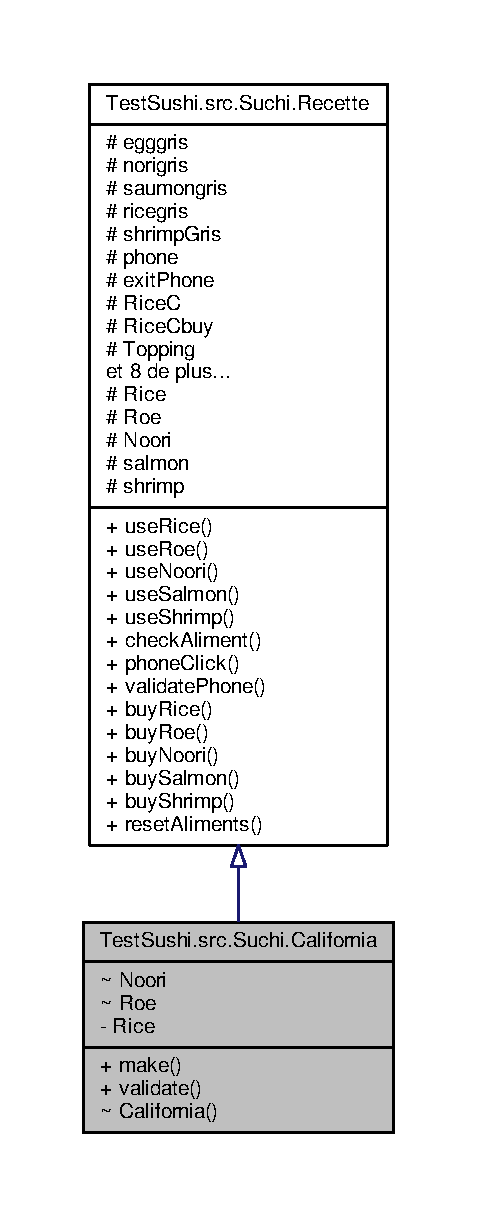
\includegraphics[height=550pt]{classTestSushi_1_1src_1_1Suchi_1_1California__inherit__graph}
\end{center}
\end{figure}


Graphe de collaboration de Test\+Sushi.\+src.\+Suchi.\+California\+:\nopagebreak
\begin{figure}[H]
\begin{center}
\leavevmode
\includegraphics[height=550pt]{classTestSushi_1_1src_1_1Suchi_1_1California__coll__graph}
\end{center}
\end{figure}
\subsubsection*{Fonctions membres publiques}
\begin{DoxyCompactItemize}
\item 
void \hyperlink{classTestSushi_1_1src_1_1Suchi_1_1California_ad90a7bbfd16b3d4b7348bde603118e8e}{make} ()  throws A\+W\+T\+Exception, Interrupted\+Exception
\item 
void \hyperlink{classTestSushi_1_1src_1_1Suchi_1_1California_a8bac6f9285749ee10208d2fc4220679f}{validate} ()  throws A\+W\+T\+Exception, Interrupted\+Exception 
\item 
void \hyperlink{classTestSushi_1_1src_1_1Suchi_1_1Recette_a2d78a4575d1295e34210e2f77c01f3f3}{use\+Rice} ()  throws A\+W\+T\+Exception, Interrupted\+Exception
\item 
void \hyperlink{classTestSushi_1_1src_1_1Suchi_1_1Recette_a8967a205e78d02ef7c30fd435fbaa0af}{use\+Roe} ()  throws A\+W\+T\+Exception, Interrupted\+Exception
\item 
void \hyperlink{classTestSushi_1_1src_1_1Suchi_1_1Recette_a10bfe3c71750c84144203a7aa2c341ee}{use\+Noori} ()  throws A\+W\+T\+Exception, Interrupted\+Exception
\item 
void \hyperlink{classTestSushi_1_1src_1_1Suchi_1_1Recette_a87cd9338767df0e5db88e6005f1da984}{use\+Salmon} ()  throws A\+W\+T\+Exception, Interrupted\+Exception
\item 
void \hyperlink{classTestSushi_1_1src_1_1Suchi_1_1Recette_ab2c165554830ba84a392765621604d44}{use\+Shrimp} ()  throws A\+W\+T\+Exception, Interrupted\+Exception
\item 
void \hyperlink{classTestSushi_1_1src_1_1Suchi_1_1Recette_a83f9f5fb6bfe2691974a5e35386e7b8a}{check\+Aliment} ()  throws A\+W\+T\+Exception, Interrupted\+Exception
\item 
void \hyperlink{classTestSushi_1_1src_1_1Suchi_1_1Recette_ad94006ea131c2379a14c50eec870b69b}{phone\+Click} ()  throws A\+W\+T\+Exception, Interrupted\+Exception
\item 
void \hyperlink{classTestSushi_1_1src_1_1Suchi_1_1Recette_a33f0912e1212b01ea1b3787bed28f0fe}{validate\+Phone} ()  throws A\+W\+T\+Exception
\item 
void \hyperlink{classTestSushi_1_1src_1_1Suchi_1_1Recette_aa0fc4c335f6ab3f905f63a16902a6379}{buy\+Rice} ()  throws A\+W\+T\+Exception, Interrupted\+Exception
\item 
void \hyperlink{classTestSushi_1_1src_1_1Suchi_1_1Recette_ad874ba9daf68328d6b65b09e6f16003e}{buy\+Roe} ()  throws A\+W\+T\+Exception, Interrupted\+Exception
\item 
void \hyperlink{classTestSushi_1_1src_1_1Suchi_1_1Recette_a5602befaaef8858b75c131e50f7cf91d}{buy\+Noori} ()  throws A\+W\+T\+Exception, Interrupted\+Exception
\item 
void \hyperlink{classTestSushi_1_1src_1_1Suchi_1_1Recette_a64cf6254490e04e9e8031d564a4a0ea3}{buy\+Salmon} ()  throws A\+W\+T\+Exception, Interrupted\+Exception
\item 
void \hyperlink{classTestSushi_1_1src_1_1Suchi_1_1Recette_a0d15202c729b3c6b2bb699de4137d551}{buy\+Shrimp} ()  throws A\+W\+T\+Exception, Interrupted\+Exception
\end{DoxyCompactItemize}
\subsubsection*{Fonctions membres publiques statiques}
\begin{DoxyCompactItemize}
\item 
static void \hyperlink{classTestSushi_1_1src_1_1Suchi_1_1Recette_aef7faa1aea5f8aeb869c612af16e4e62}{reset\+Aliments} ()
\end{DoxyCompactItemize}
\subsubsection*{Attributs protégés}
\begin{DoxyCompactItemize}
\item 
final String \hyperlink{classTestSushi_1_1src_1_1Suchi_1_1Recette_a14892e43d9ed57350effdf3ed1bddb8a}{egggris} = \char`\"{}sprites/egg\+Gris.\+png\char`\"{}
\item 
final String \hyperlink{classTestSushi_1_1src_1_1Suchi_1_1Recette_a774959efa525787a162778df37770b7c}{norigris} = \char`\"{}sprites/nori\+Gris.\+png\char`\"{}
\item 
final String \hyperlink{classTestSushi_1_1src_1_1Suchi_1_1Recette_aea59cc2a5f6bc21ec36690a5bf1eb38c}{saumongris} =\char`\"{}sprites/saumon\+Gris.\+png\char`\"{}
\item 
final String \hyperlink{classTestSushi_1_1src_1_1Suchi_1_1Recette_a616939eea675e05aa6d7ec62fd90f461}{ricegris} = \char`\"{}sprites/rice\+Gris.\+png\char`\"{}
\item 
final String \hyperlink{classTestSushi_1_1src_1_1Suchi_1_1Recette_ac1b1b9b91dba95a9d0df2f6e59f04a59}{shrimp\+Gris} = \char`\"{}sprites/shrimp\+Gris.\+png\char`\"{}
\item 
final Point \hyperlink{classTestSushi_1_1src_1_1Suchi_1_1Recette_a45e48b1a85957813f1a747df04923b08}{phone} = new Point (1030,620)
\item 
final Point \hyperlink{classTestSushi_1_1src_1_1Suchi_1_1Recette_aecc6de3619013f1fb5f506c1e4e9ad7b}{exit\+Phone} = new Point (1050,573)
\item 
final Point \hyperlink{classTestSushi_1_1src_1_1Suchi_1_1Recette_ab502e1d023a0bd3fadfc714e1babc728}{Rice\+C} = new Point (973,503)
\item 
final Point \hyperlink{classTestSushi_1_1src_1_1Suchi_1_1Recette_a890dce3bb5d54a700fa7bebc2496e931}{Rice\+Cbuy} = new Point (976,487)
\item 
final Point \hyperlink{classTestSushi_1_1src_1_1Suchi_1_1Recette_ab7575f64998864f6b053859c18380f58}{Topping} = new Point (978,470)
\item 
final Point \hyperlink{classTestSushi_1_1src_1_1Suchi_1_1Recette_a2f5cec48c186dc52c3d990df66f3a8cf}{fish\+Eggs} = new Point (979,472)
\item 
final Point \hyperlink{classTestSushi_1_1src_1_1Suchi_1_1Recette_a4f3e62b4ab32fcc5d8b6875996f47618}{nori} = new Point (929,469)
\item 
final Point \hyperlink{classTestSushi_1_1src_1_1Suchi_1_1Recette_a9c491e7f09a444817e433e54923e6bca}{validate} = new Point (900,500)
\item 
final Point \hyperlink{classTestSushi_1_1src_1_1Suchi_1_1Recette_a855a7ed217eec3565619156fa6cd4214}{saumon} = new Point (910,560)
\item 
final Point \hyperlink{classTestSushi_1_1src_1_1Suchi_1_1Recette_a69faeadec2c0d475bbd77c3b7eeaada7}{shrimp\+Coord} = new Point (907,386)
\item 
final int \hyperlink{classTestSushi_1_1src_1_1Suchi_1_1Recette_a2c78759553661a7e4b01d4ac1212ec6c}{time} = 150
\item 
final int \hyperlink{classTestSushi_1_1src_1_1Suchi_1_1Recette_a0d95a4a68ee0d423b6815b296f3304b2}{phone\+Time} = 50
\item 
final int \hyperlink{classTestSushi_1_1src_1_1Suchi_1_1Recette_a7db8ec6383e36487bc7ca0490edd0b4a}{time\+Tapis} = 650
\end{DoxyCompactItemize}
\subsubsection*{Attributs protégés statiques}
\begin{DoxyCompactItemize}
\item 
static int \hyperlink{classTestSushi_1_1src_1_1Suchi_1_1Recette_a726a712fe936ef2a96982e00d21c49c0}{salmon} = 5
\item 
static int \hyperlink{classTestSushi_1_1src_1_1Suchi_1_1Recette_a07fa939a0df1b7ff45a9d4aa77498e8e}{shrimp} = 5
\end{DoxyCompactItemize}
\subsubsection*{Fonctions de paquetage}
\begin{DoxyCompactItemize}
\item 
\hyperlink{classTestSushi_1_1src_1_1Suchi_1_1California_a634f2d6d5654850c742733e9649f2d06}{California} ()  throws A\+W\+T\+Exception, Interrupted\+Exception 
\begin{DoxyCompactList}\small\item\em Constructeur, va appeller les différentes méthodes pour créer un california. \end{DoxyCompactList}\end{DoxyCompactItemize}
\subsubsection*{Attributs de paquetage}
\begin{DoxyCompactItemize}
\item 
Point \hyperlink{classTestSushi_1_1src_1_1Suchi_1_1California_a0a9bb5b64454647e04a23e0ef47ad3b6}{Noori}
\item 
Point \hyperlink{classTestSushi_1_1src_1_1Suchi_1_1California_a4bfdebd854fd95d3113f192322a542ff}{Roe}
\end{DoxyCompactItemize}
\subsubsection*{Attributs privés}
\begin{DoxyCompactItemize}
\item 
Point \hyperlink{classTestSushi_1_1src_1_1Suchi_1_1California_a73e9074a8d90df58d326b4c872254bda}{Rice}
\end{DoxyCompactItemize}


\subsubsection{Documentation des constructeurs et destructeur}
\hypertarget{classTestSushi_1_1src_1_1Suchi_1_1California_a634f2d6d5654850c742733e9649f2d06}{}\index{Test\+Sushi\+::src\+::\+Suchi\+::\+California@{Test\+Sushi\+::src\+::\+Suchi\+::\+California}!California@{California}}
\index{California@{California}!Test\+Sushi\+::src\+::\+Suchi\+::\+California@{Test\+Sushi\+::src\+::\+Suchi\+::\+California}}
\paragraph[{California}]{\setlength{\rightskip}{0pt plus 5cm}Test\+Sushi.\+src.\+Suchi.\+California.\+California (
\begin{DoxyParamCaption}
{}
\end{DoxyParamCaption}
) throws A\+W\+T\+Exception, Interrupted\+Exception\hspace{0.3cm}{\ttfamily [package]}}\label{classTestSushi_1_1src_1_1Suchi_1_1California_a634f2d6d5654850c742733e9649f2d06}


Constructeur, va appeller les différentes méthodes pour créer un california. 


\begin{DoxyExceptions}{Exceptions}
{\em A\+W\+T\+Exception} & \\
\hline
{\em Interrupted\+Exception} & \\
\hline
\end{DoxyExceptions}


\subsubsection{Documentation des fonctions membres}
\hypertarget{classTestSushi_1_1src_1_1Suchi_1_1Recette_a5602befaaef8858b75c131e50f7cf91d}{}\index{Test\+Sushi\+::src\+::\+Suchi\+::\+California@{Test\+Sushi\+::src\+::\+Suchi\+::\+California}!buy\+Noori@{buy\+Noori}}
\index{buy\+Noori@{buy\+Noori}!Test\+Sushi\+::src\+::\+Suchi\+::\+California@{Test\+Sushi\+::src\+::\+Suchi\+::\+California}}
\paragraph[{buy\+Noori}]{\setlength{\rightskip}{0pt plus 5cm}void Test\+Sushi.\+src.\+Suchi.\+Recette.\+buy\+Noori (
\begin{DoxyParamCaption}
{}
\end{DoxyParamCaption}
) throws A\+W\+T\+Exception, Interrupted\+Exception\hspace{0.3cm}{\ttfamily [inherited]}}\label{classTestSushi_1_1src_1_1Suchi_1_1Recette_a5602befaaef8858b75c131e50f7cf91d}

\begin{DoxyExceptions}{Exceptions}
{\em A\+W\+T\+Exception} & \\
\hline
{\em Interrupted\+Exception} & \\
\hline
\end{DoxyExceptions}


Référencé par Test\+Sushi.\+src.\+Suchi.\+Recette.\+check\+Aliment().

\hypertarget{classTestSushi_1_1src_1_1Suchi_1_1Recette_aa0fc4c335f6ab3f905f63a16902a6379}{}\index{Test\+Sushi\+::src\+::\+Suchi\+::\+California@{Test\+Sushi\+::src\+::\+Suchi\+::\+California}!buy\+Rice@{buy\+Rice}}
\index{buy\+Rice@{buy\+Rice}!Test\+Sushi\+::src\+::\+Suchi\+::\+California@{Test\+Sushi\+::src\+::\+Suchi\+::\+California}}
\paragraph[{buy\+Rice}]{\setlength{\rightskip}{0pt plus 5cm}void Test\+Sushi.\+src.\+Suchi.\+Recette.\+buy\+Rice (
\begin{DoxyParamCaption}
{}
\end{DoxyParamCaption}
) throws A\+W\+T\+Exception, Interrupted\+Exception\hspace{0.3cm}{\ttfamily [inherited]}}\label{classTestSushi_1_1src_1_1Suchi_1_1Recette_aa0fc4c335f6ab3f905f63a16902a6379}

\begin{DoxyExceptions}{Exceptions}
{\em A\+W\+T\+Exception} & \\
\hline
{\em Interrupted\+Exception} & \\
\hline
\end{DoxyExceptions}


Référencé par Test\+Sushi.\+src.\+Suchi.\+Recette.\+check\+Aliment().

\hypertarget{classTestSushi_1_1src_1_1Suchi_1_1Recette_ad874ba9daf68328d6b65b09e6f16003e}{}\index{Test\+Sushi\+::src\+::\+Suchi\+::\+California@{Test\+Sushi\+::src\+::\+Suchi\+::\+California}!buy\+Roe@{buy\+Roe}}
\index{buy\+Roe@{buy\+Roe}!Test\+Sushi\+::src\+::\+Suchi\+::\+California@{Test\+Sushi\+::src\+::\+Suchi\+::\+California}}
\paragraph[{buy\+Roe}]{\setlength{\rightskip}{0pt plus 5cm}void Test\+Sushi.\+src.\+Suchi.\+Recette.\+buy\+Roe (
\begin{DoxyParamCaption}
{}
\end{DoxyParamCaption}
) throws A\+W\+T\+Exception, Interrupted\+Exception\hspace{0.3cm}{\ttfamily [inherited]}}\label{classTestSushi_1_1src_1_1Suchi_1_1Recette_ad874ba9daf68328d6b65b09e6f16003e}

\begin{DoxyExceptions}{Exceptions}
{\em A\+W\+T\+Exception} & \\
\hline
{\em Interrupted\+Exception} & \\
\hline
\end{DoxyExceptions}


Référencé par Test\+Sushi.\+src.\+Suchi.\+Recette.\+check\+Aliment().

\hypertarget{classTestSushi_1_1src_1_1Suchi_1_1Recette_a64cf6254490e04e9e8031d564a4a0ea3}{}\index{Test\+Sushi\+::src\+::\+Suchi\+::\+California@{Test\+Sushi\+::src\+::\+Suchi\+::\+California}!buy\+Salmon@{buy\+Salmon}}
\index{buy\+Salmon@{buy\+Salmon}!Test\+Sushi\+::src\+::\+Suchi\+::\+California@{Test\+Sushi\+::src\+::\+Suchi\+::\+California}}
\paragraph[{buy\+Salmon}]{\setlength{\rightskip}{0pt plus 5cm}void Test\+Sushi.\+src.\+Suchi.\+Recette.\+buy\+Salmon (
\begin{DoxyParamCaption}
{}
\end{DoxyParamCaption}
) throws A\+W\+T\+Exception, Interrupted\+Exception\hspace{0.3cm}{\ttfamily [inherited]}}\label{classTestSushi_1_1src_1_1Suchi_1_1Recette_a64cf6254490e04e9e8031d564a4a0ea3}

\begin{DoxyExceptions}{Exceptions}
{\em A\+W\+T\+Exception} & \\
\hline
{\em Interrupted\+Exception} & \\
\hline
\end{DoxyExceptions}


Référencé par Test\+Sushi.\+src.\+Suchi.\+Recette.\+check\+Aliment().

\hypertarget{classTestSushi_1_1src_1_1Suchi_1_1Recette_a0d15202c729b3c6b2bb699de4137d551}{}\index{Test\+Sushi\+::src\+::\+Suchi\+::\+California@{Test\+Sushi\+::src\+::\+Suchi\+::\+California}!buy\+Shrimp@{buy\+Shrimp}}
\index{buy\+Shrimp@{buy\+Shrimp}!Test\+Sushi\+::src\+::\+Suchi\+::\+California@{Test\+Sushi\+::src\+::\+Suchi\+::\+California}}
\paragraph[{buy\+Shrimp}]{\setlength{\rightskip}{0pt plus 5cm}void Test\+Sushi.\+src.\+Suchi.\+Recette.\+buy\+Shrimp (
\begin{DoxyParamCaption}
{}
\end{DoxyParamCaption}
) throws A\+W\+T\+Exception, Interrupted\+Exception\hspace{0.3cm}{\ttfamily [inherited]}}\label{classTestSushi_1_1src_1_1Suchi_1_1Recette_a0d15202c729b3c6b2bb699de4137d551}

\begin{DoxyExceptions}{Exceptions}
{\em A\+W\+T\+Exception} & \\
\hline
{\em Interrupted\+Exception} & \\
\hline
\end{DoxyExceptions}


Référencé par Test\+Sushi.\+src.\+Suchi.\+Recette.\+check\+Aliment().

\hypertarget{classTestSushi_1_1src_1_1Suchi_1_1Recette_a83f9f5fb6bfe2691974a5e35386e7b8a}{}\index{Test\+Sushi\+::src\+::\+Suchi\+::\+California@{Test\+Sushi\+::src\+::\+Suchi\+::\+California}!check\+Aliment@{check\+Aliment}}
\index{check\+Aliment@{check\+Aliment}!Test\+Sushi\+::src\+::\+Suchi\+::\+California@{Test\+Sushi\+::src\+::\+Suchi\+::\+California}}
\paragraph[{check\+Aliment}]{\setlength{\rightskip}{0pt plus 5cm}void Test\+Sushi.\+src.\+Suchi.\+Recette.\+check\+Aliment (
\begin{DoxyParamCaption}
{}
\end{DoxyParamCaption}
) throws A\+W\+T\+Exception, Interrupted\+Exception\hspace{0.3cm}{\ttfamily [inherited]}}\label{classTestSushi_1_1src_1_1Suchi_1_1Recette_a83f9f5fb6bfe2691974a5e35386e7b8a}

\begin{DoxyExceptions}{Exceptions}
{\em A\+W\+T\+Exception} & \\
\hline
{\em Interrupted\+Exception} & \\
\hline
\end{DoxyExceptions}


Référencé par Test\+Sushi.\+src.\+Suchi.\+Recette.\+use\+Noori(), Test\+Sushi.\+src.\+Suchi.\+Recette.\+use\+Rice(), Test\+Sushi.\+src.\+Suchi.\+Recette.\+use\+Roe(), Test\+Sushi.\+src.\+Suchi.\+Recette.\+use\+Salmon(), et Test\+Sushi.\+src.\+Suchi.\+Recette.\+use\+Shrimp().

\hypertarget{classTestSushi_1_1src_1_1Suchi_1_1California_ad90a7bbfd16b3d4b7348bde603118e8e}{}\index{Test\+Sushi\+::src\+::\+Suchi\+::\+California@{Test\+Sushi\+::src\+::\+Suchi\+::\+California}!make@{make}}
\index{make@{make}!Test\+Sushi\+::src\+::\+Suchi\+::\+California@{Test\+Sushi\+::src\+::\+Suchi\+::\+California}}
\paragraph[{make}]{\setlength{\rightskip}{0pt plus 5cm}void Test\+Sushi.\+src.\+Suchi.\+California.\+make (
\begin{DoxyParamCaption}
{}
\end{DoxyParamCaption}
) throws A\+W\+T\+Exception, Interrupted\+Exception}\label{classTestSushi_1_1src_1_1Suchi_1_1California_ad90a7bbfd16b3d4b7348bde603118e8e}

\begin{DoxyExceptions}{Exceptions}
{\em A\+W\+T\+Exception} & \\
\hline
{\em Interrupted\+Exception} & \\
\hline
\end{DoxyExceptions}


Référencé par Test\+Sushi.\+src.\+Suchi.\+California.\+California().

\hypertarget{classTestSushi_1_1src_1_1Suchi_1_1Recette_ad94006ea131c2379a14c50eec870b69b}{}\index{Test\+Sushi\+::src\+::\+Suchi\+::\+California@{Test\+Sushi\+::src\+::\+Suchi\+::\+California}!phone\+Click@{phone\+Click}}
\index{phone\+Click@{phone\+Click}!Test\+Sushi\+::src\+::\+Suchi\+::\+California@{Test\+Sushi\+::src\+::\+Suchi\+::\+California}}
\paragraph[{phone\+Click}]{\setlength{\rightskip}{0pt plus 5cm}void Test\+Sushi.\+src.\+Suchi.\+Recette.\+phone\+Click (
\begin{DoxyParamCaption}
{}
\end{DoxyParamCaption}
) throws A\+W\+T\+Exception, Interrupted\+Exception\hspace{0.3cm}{\ttfamily [inherited]}}\label{classTestSushi_1_1src_1_1Suchi_1_1Recette_ad94006ea131c2379a14c50eec870b69b}

\begin{DoxyExceptions}{Exceptions}
{\em A\+W\+T\+Exception} & \\
\hline
{\em Interrupted\+Exception} & \\
\hline
\end{DoxyExceptions}


Référencé par Test\+Sushi.\+src.\+Suchi.\+Recette.\+buy\+Noori(), Test\+Sushi.\+src.\+Suchi.\+Recette.\+buy\+Rice(), Test\+Sushi.\+src.\+Suchi.\+Recette.\+buy\+Roe(), Test\+Sushi.\+src.\+Suchi.\+Recette.\+buy\+Salmon(), et Test\+Sushi.\+src.\+Suchi.\+Recette.\+buy\+Shrimp().

\hypertarget{classTestSushi_1_1src_1_1Suchi_1_1Recette_aef7faa1aea5f8aeb869c612af16e4e62}{}\index{Test\+Sushi\+::src\+::\+Suchi\+::\+California@{Test\+Sushi\+::src\+::\+Suchi\+::\+California}!reset\+Aliments@{reset\+Aliments}}
\index{reset\+Aliments@{reset\+Aliments}!Test\+Sushi\+::src\+::\+Suchi\+::\+California@{Test\+Sushi\+::src\+::\+Suchi\+::\+California}}
\paragraph[{reset\+Aliments}]{\setlength{\rightskip}{0pt plus 5cm}static void Test\+Sushi.\+src.\+Suchi.\+Recette.\+reset\+Aliments (
\begin{DoxyParamCaption}
{}
\end{DoxyParamCaption}
)\hspace{0.3cm}{\ttfamily [static]}, {\ttfamily [inherited]}}\label{classTestSushi_1_1src_1_1Suchi_1_1Recette_aef7faa1aea5f8aeb869c612af16e4e62}


Référencé par Test\+Sushi.\+src.\+Suchi.\+Game.\+start\+Level2(), et Test\+Sushi.\+src.\+Suchi.\+Game.\+start\+Level3().

\hypertarget{classTestSushi_1_1src_1_1Suchi_1_1Recette_a10bfe3c71750c84144203a7aa2c341ee}{}\index{Test\+Sushi\+::src\+::\+Suchi\+::\+California@{Test\+Sushi\+::src\+::\+Suchi\+::\+California}!use\+Noori@{use\+Noori}}
\index{use\+Noori@{use\+Noori}!Test\+Sushi\+::src\+::\+Suchi\+::\+California@{Test\+Sushi\+::src\+::\+Suchi\+::\+California}}
\paragraph[{use\+Noori}]{\setlength{\rightskip}{0pt plus 5cm}void Test\+Sushi.\+src.\+Suchi.\+Recette.\+use\+Noori (
\begin{DoxyParamCaption}
{}
\end{DoxyParamCaption}
) throws A\+W\+T\+Exception, Interrupted\+Exception\hspace{0.3cm}{\ttfamily [inherited]}}\label{classTestSushi_1_1src_1_1Suchi_1_1Recette_a10bfe3c71750c84144203a7aa2c341ee}

\begin{DoxyExceptions}{Exceptions}
{\em A\+W\+T\+Exception} & \\
\hline
{\em Interrupted\+Exception} & \\
\hline
\end{DoxyExceptions}
\hypertarget{classTestSushi_1_1src_1_1Suchi_1_1Recette_a2d78a4575d1295e34210e2f77c01f3f3}{}\index{Test\+Sushi\+::src\+::\+Suchi\+::\+California@{Test\+Sushi\+::src\+::\+Suchi\+::\+California}!use\+Rice@{use\+Rice}}
\index{use\+Rice@{use\+Rice}!Test\+Sushi\+::src\+::\+Suchi\+::\+California@{Test\+Sushi\+::src\+::\+Suchi\+::\+California}}
\paragraph[{use\+Rice}]{\setlength{\rightskip}{0pt plus 5cm}void Test\+Sushi.\+src.\+Suchi.\+Recette.\+use\+Rice (
\begin{DoxyParamCaption}
{}
\end{DoxyParamCaption}
) throws A\+W\+T\+Exception, Interrupted\+Exception\hspace{0.3cm}{\ttfamily [inherited]}}\label{classTestSushi_1_1src_1_1Suchi_1_1Recette_a2d78a4575d1295e34210e2f77c01f3f3}

\begin{DoxyExceptions}{Exceptions}
{\em A\+W\+T\+Exception} & \\
\hline
{\em Interrupted\+Exception} & \\
\hline
\end{DoxyExceptions}
\hypertarget{classTestSushi_1_1src_1_1Suchi_1_1Recette_a8967a205e78d02ef7c30fd435fbaa0af}{}\index{Test\+Sushi\+::src\+::\+Suchi\+::\+California@{Test\+Sushi\+::src\+::\+Suchi\+::\+California}!use\+Roe@{use\+Roe}}
\index{use\+Roe@{use\+Roe}!Test\+Sushi\+::src\+::\+Suchi\+::\+California@{Test\+Sushi\+::src\+::\+Suchi\+::\+California}}
\paragraph[{use\+Roe}]{\setlength{\rightskip}{0pt plus 5cm}void Test\+Sushi.\+src.\+Suchi.\+Recette.\+use\+Roe (
\begin{DoxyParamCaption}
{}
\end{DoxyParamCaption}
) throws A\+W\+T\+Exception, Interrupted\+Exception\hspace{0.3cm}{\ttfamily [inherited]}}\label{classTestSushi_1_1src_1_1Suchi_1_1Recette_a8967a205e78d02ef7c30fd435fbaa0af}

\begin{DoxyExceptions}{Exceptions}
{\em A\+W\+T\+Exception} & \\
\hline
{\em Interrupted\+Exception} & \\
\hline
\end{DoxyExceptions}
\hypertarget{classTestSushi_1_1src_1_1Suchi_1_1Recette_a87cd9338767df0e5db88e6005f1da984}{}\index{Test\+Sushi\+::src\+::\+Suchi\+::\+California@{Test\+Sushi\+::src\+::\+Suchi\+::\+California}!use\+Salmon@{use\+Salmon}}
\index{use\+Salmon@{use\+Salmon}!Test\+Sushi\+::src\+::\+Suchi\+::\+California@{Test\+Sushi\+::src\+::\+Suchi\+::\+California}}
\paragraph[{use\+Salmon}]{\setlength{\rightskip}{0pt plus 5cm}void Test\+Sushi.\+src.\+Suchi.\+Recette.\+use\+Salmon (
\begin{DoxyParamCaption}
{}
\end{DoxyParamCaption}
) throws A\+W\+T\+Exception, Interrupted\+Exception\hspace{0.3cm}{\ttfamily [inherited]}}\label{classTestSushi_1_1src_1_1Suchi_1_1Recette_a87cd9338767df0e5db88e6005f1da984}

\begin{DoxyExceptions}{Exceptions}
{\em A\+W\+T\+Exception} & \\
\hline
{\em Interrupted\+Exception} & \\
\hline
\end{DoxyExceptions}
\hypertarget{classTestSushi_1_1src_1_1Suchi_1_1Recette_ab2c165554830ba84a392765621604d44}{}\index{Test\+Sushi\+::src\+::\+Suchi\+::\+California@{Test\+Sushi\+::src\+::\+Suchi\+::\+California}!use\+Shrimp@{use\+Shrimp}}
\index{use\+Shrimp@{use\+Shrimp}!Test\+Sushi\+::src\+::\+Suchi\+::\+California@{Test\+Sushi\+::src\+::\+Suchi\+::\+California}}
\paragraph[{use\+Shrimp}]{\setlength{\rightskip}{0pt plus 5cm}void Test\+Sushi.\+src.\+Suchi.\+Recette.\+use\+Shrimp (
\begin{DoxyParamCaption}
{}
\end{DoxyParamCaption}
) throws A\+W\+T\+Exception, Interrupted\+Exception\hspace{0.3cm}{\ttfamily [inherited]}}\label{classTestSushi_1_1src_1_1Suchi_1_1Recette_ab2c165554830ba84a392765621604d44}

\begin{DoxyExceptions}{Exceptions}
{\em A\+W\+T\+Exception} & \\
\hline
{\em Interrupted\+Exception} & \\
\hline
\end{DoxyExceptions}
\hypertarget{classTestSushi_1_1src_1_1Suchi_1_1California_a8bac6f9285749ee10208d2fc4220679f}{}\index{Test\+Sushi\+::src\+::\+Suchi\+::\+California@{Test\+Sushi\+::src\+::\+Suchi\+::\+California}!validate@{validate}}
\index{validate@{validate}!Test\+Sushi\+::src\+::\+Suchi\+::\+California@{Test\+Sushi\+::src\+::\+Suchi\+::\+California}}
\paragraph[{validate}]{\setlength{\rightskip}{0pt plus 5cm}void Test\+Sushi.\+src.\+Suchi.\+California.\+validate (
\begin{DoxyParamCaption}
{}
\end{DoxyParamCaption}
) throws A\+W\+T\+Exception, Interrupted\+Exception}\label{classTestSushi_1_1src_1_1Suchi_1_1California_a8bac6f9285749ee10208d2fc4220679f}

\begin{DoxyExceptions}{Exceptions}
{\em A\+W\+T\+Exception} & \\
\hline
{\em Interrupted\+Exception} & \\
\hline
\end{DoxyExceptions}


Référencé par Test\+Sushi.\+src.\+Suchi.\+California.\+California().

\hypertarget{classTestSushi_1_1src_1_1Suchi_1_1Recette_a33f0912e1212b01ea1b3787bed28f0fe}{}\index{Test\+Sushi\+::src\+::\+Suchi\+::\+California@{Test\+Sushi\+::src\+::\+Suchi\+::\+California}!validate\+Phone@{validate\+Phone}}
\index{validate\+Phone@{validate\+Phone}!Test\+Sushi\+::src\+::\+Suchi\+::\+California@{Test\+Sushi\+::src\+::\+Suchi\+::\+California}}
\paragraph[{validate\+Phone}]{\setlength{\rightskip}{0pt plus 5cm}void Test\+Sushi.\+src.\+Suchi.\+Recette.\+validate\+Phone (
\begin{DoxyParamCaption}
{}
\end{DoxyParamCaption}
) throws A\+W\+T\+Exception\hspace{0.3cm}{\ttfamily [inherited]}}\label{classTestSushi_1_1src_1_1Suchi_1_1Recette_a33f0912e1212b01ea1b3787bed28f0fe}

\begin{DoxyExceptions}{Exceptions}
{\em A\+W\+T\+Exception} & \\
\hline
\end{DoxyExceptions}


Référencé par Test\+Sushi.\+src.\+Suchi.\+Recette.\+buy\+Noori(), Test\+Sushi.\+src.\+Suchi.\+Recette.\+buy\+Rice(), Test\+Sushi.\+src.\+Suchi.\+Recette.\+buy\+Roe(), Test\+Sushi.\+src.\+Suchi.\+Recette.\+buy\+Salmon(), et Test\+Sushi.\+src.\+Suchi.\+Recette.\+buy\+Shrimp().



\subsubsection{Documentation des données membres}
\hypertarget{classTestSushi_1_1src_1_1Suchi_1_1Recette_a14892e43d9ed57350effdf3ed1bddb8a}{}\index{Test\+Sushi\+::src\+::\+Suchi\+::\+California@{Test\+Sushi\+::src\+::\+Suchi\+::\+California}!egggris@{egggris}}
\index{egggris@{egggris}!Test\+Sushi\+::src\+::\+Suchi\+::\+California@{Test\+Sushi\+::src\+::\+Suchi\+::\+California}}
\paragraph[{egggris}]{\setlength{\rightskip}{0pt plus 5cm}final String Test\+Sushi.\+src.\+Suchi.\+Recette.\+egggris = \char`\"{}sprites/egg\+Gris.\+png\char`\"{}\hspace{0.3cm}{\ttfamily [protected]}, {\ttfamily [inherited]}}\label{classTestSushi_1_1src_1_1Suchi_1_1Recette_a14892e43d9ed57350effdf3ed1bddb8a}


Référencé par Test\+Sushi.\+src.\+Suchi.\+Recette.\+buy\+Roe().

\hypertarget{classTestSushi_1_1src_1_1Suchi_1_1Recette_aecc6de3619013f1fb5f506c1e4e9ad7b}{}\index{Test\+Sushi\+::src\+::\+Suchi\+::\+California@{Test\+Sushi\+::src\+::\+Suchi\+::\+California}!exit\+Phone@{exit\+Phone}}
\index{exit\+Phone@{exit\+Phone}!Test\+Sushi\+::src\+::\+Suchi\+::\+California@{Test\+Sushi\+::src\+::\+Suchi\+::\+California}}
\paragraph[{exit\+Phone}]{\setlength{\rightskip}{0pt plus 5cm}final Point Test\+Sushi.\+src.\+Suchi.\+Recette.\+exit\+Phone = new Point (1050,573)\hspace{0.3cm}{\ttfamily [protected]}, {\ttfamily [inherited]}}\label{classTestSushi_1_1src_1_1Suchi_1_1Recette_aecc6de3619013f1fb5f506c1e4e9ad7b}
\hypertarget{classTestSushi_1_1src_1_1Suchi_1_1Recette_a2f5cec48c186dc52c3d990df66f3a8cf}{}\index{Test\+Sushi\+::src\+::\+Suchi\+::\+California@{Test\+Sushi\+::src\+::\+Suchi\+::\+California}!fish\+Eggs@{fish\+Eggs}}
\index{fish\+Eggs@{fish\+Eggs}!Test\+Sushi\+::src\+::\+Suchi\+::\+California@{Test\+Sushi\+::src\+::\+Suchi\+::\+California}}
\paragraph[{fish\+Eggs}]{\setlength{\rightskip}{0pt plus 5cm}final Point Test\+Sushi.\+src.\+Suchi.\+Recette.\+fish\+Eggs = new Point (979,472)\hspace{0.3cm}{\ttfamily [protected]}, {\ttfamily [inherited]}}\label{classTestSushi_1_1src_1_1Suchi_1_1Recette_a2f5cec48c186dc52c3d990df66f3a8cf}
\hypertarget{classTestSushi_1_1src_1_1Suchi_1_1California_a0a9bb5b64454647e04a23e0ef47ad3b6}{}\index{Test\+Sushi\+::src\+::\+Suchi\+::\+California@{Test\+Sushi\+::src\+::\+Suchi\+::\+California}!Noori@{Noori}}
\index{Noori@{Noori}!Test\+Sushi\+::src\+::\+Suchi\+::\+California@{Test\+Sushi\+::src\+::\+Suchi\+::\+California}}
\paragraph[{Noori}]{\setlength{\rightskip}{0pt plus 5cm}Point Test\+Sushi.\+src.\+Suchi.\+California.\+Noori\hspace{0.3cm}{\ttfamily [package]}}\label{classTestSushi_1_1src_1_1Suchi_1_1California_a0a9bb5b64454647e04a23e0ef47ad3b6}
\hypertarget{classTestSushi_1_1src_1_1Suchi_1_1Recette_a4f3e62b4ab32fcc5d8b6875996f47618}{}\index{Test\+Sushi\+::src\+::\+Suchi\+::\+California@{Test\+Sushi\+::src\+::\+Suchi\+::\+California}!nori@{nori}}
\index{nori@{nori}!Test\+Sushi\+::src\+::\+Suchi\+::\+California@{Test\+Sushi\+::src\+::\+Suchi\+::\+California}}
\paragraph[{nori}]{\setlength{\rightskip}{0pt plus 5cm}final Point Test\+Sushi.\+src.\+Suchi.\+Recette.\+nori = new Point (929,469)\hspace{0.3cm}{\ttfamily [protected]}, {\ttfamily [inherited]}}\label{classTestSushi_1_1src_1_1Suchi_1_1Recette_a4f3e62b4ab32fcc5d8b6875996f47618}
\hypertarget{classTestSushi_1_1src_1_1Suchi_1_1Recette_a774959efa525787a162778df37770b7c}{}\index{Test\+Sushi\+::src\+::\+Suchi\+::\+California@{Test\+Sushi\+::src\+::\+Suchi\+::\+California}!norigris@{norigris}}
\index{norigris@{norigris}!Test\+Sushi\+::src\+::\+Suchi\+::\+California@{Test\+Sushi\+::src\+::\+Suchi\+::\+California}}
\paragraph[{norigris}]{\setlength{\rightskip}{0pt plus 5cm}final String Test\+Sushi.\+src.\+Suchi.\+Recette.\+norigris = \char`\"{}sprites/nori\+Gris.\+png\char`\"{}\hspace{0.3cm}{\ttfamily [protected]}, {\ttfamily [inherited]}}\label{classTestSushi_1_1src_1_1Suchi_1_1Recette_a774959efa525787a162778df37770b7c}


Référencé par Test\+Sushi.\+src.\+Suchi.\+Recette.\+buy\+Noori().

\hypertarget{classTestSushi_1_1src_1_1Suchi_1_1Recette_a45e48b1a85957813f1a747df04923b08}{}\index{Test\+Sushi\+::src\+::\+Suchi\+::\+California@{Test\+Sushi\+::src\+::\+Suchi\+::\+California}!phone@{phone}}
\index{phone@{phone}!Test\+Sushi\+::src\+::\+Suchi\+::\+California@{Test\+Sushi\+::src\+::\+Suchi\+::\+California}}
\paragraph[{phone}]{\setlength{\rightskip}{0pt plus 5cm}final Point Test\+Sushi.\+src.\+Suchi.\+Recette.\+phone = new Point (1030,620)\hspace{0.3cm}{\ttfamily [protected]}, {\ttfamily [inherited]}}\label{classTestSushi_1_1src_1_1Suchi_1_1Recette_a45e48b1a85957813f1a747df04923b08}
\hypertarget{classTestSushi_1_1src_1_1Suchi_1_1Recette_a0d95a4a68ee0d423b6815b296f3304b2}{}\index{Test\+Sushi\+::src\+::\+Suchi\+::\+California@{Test\+Sushi\+::src\+::\+Suchi\+::\+California}!phone\+Time@{phone\+Time}}
\index{phone\+Time@{phone\+Time}!Test\+Sushi\+::src\+::\+Suchi\+::\+California@{Test\+Sushi\+::src\+::\+Suchi\+::\+California}}
\paragraph[{phone\+Time}]{\setlength{\rightskip}{0pt plus 5cm}final int Test\+Sushi.\+src.\+Suchi.\+Recette.\+phone\+Time = 50\hspace{0.3cm}{\ttfamily [protected]}, {\ttfamily [inherited]}}\label{classTestSushi_1_1src_1_1Suchi_1_1Recette_a0d95a4a68ee0d423b6815b296f3304b2}
\hypertarget{classTestSushi_1_1src_1_1Suchi_1_1California_a73e9074a8d90df58d326b4c872254bda}{}\index{Test\+Sushi\+::src\+::\+Suchi\+::\+California@{Test\+Sushi\+::src\+::\+Suchi\+::\+California}!Rice@{Rice}}
\index{Rice@{Rice}!Test\+Sushi\+::src\+::\+Suchi\+::\+California@{Test\+Sushi\+::src\+::\+Suchi\+::\+California}}
\paragraph[{Rice}]{\setlength{\rightskip}{0pt plus 5cm}Point Test\+Sushi.\+src.\+Suchi.\+California.\+Rice\hspace{0.3cm}{\ttfamily [private]}}\label{classTestSushi_1_1src_1_1Suchi_1_1California_a73e9074a8d90df58d326b4c872254bda}
\hypertarget{classTestSushi_1_1src_1_1Suchi_1_1Recette_ab502e1d023a0bd3fadfc714e1babc728}{}\index{Test\+Sushi\+::src\+::\+Suchi\+::\+California@{Test\+Sushi\+::src\+::\+Suchi\+::\+California}!Rice\+C@{Rice\+C}}
\index{Rice\+C@{Rice\+C}!Test\+Sushi\+::src\+::\+Suchi\+::\+California@{Test\+Sushi\+::src\+::\+Suchi\+::\+California}}
\paragraph[{Rice\+C}]{\setlength{\rightskip}{0pt plus 5cm}final Point Test\+Sushi.\+src.\+Suchi.\+Recette.\+Rice\+C = new Point (973,503)\hspace{0.3cm}{\ttfamily [protected]}, {\ttfamily [inherited]}}\label{classTestSushi_1_1src_1_1Suchi_1_1Recette_ab502e1d023a0bd3fadfc714e1babc728}
\hypertarget{classTestSushi_1_1src_1_1Suchi_1_1Recette_a890dce3bb5d54a700fa7bebc2496e931}{}\index{Test\+Sushi\+::src\+::\+Suchi\+::\+California@{Test\+Sushi\+::src\+::\+Suchi\+::\+California}!Rice\+Cbuy@{Rice\+Cbuy}}
\index{Rice\+Cbuy@{Rice\+Cbuy}!Test\+Sushi\+::src\+::\+Suchi\+::\+California@{Test\+Sushi\+::src\+::\+Suchi\+::\+California}}
\paragraph[{Rice\+Cbuy}]{\setlength{\rightskip}{0pt plus 5cm}final Point Test\+Sushi.\+src.\+Suchi.\+Recette.\+Rice\+Cbuy = new Point (976,487)\hspace{0.3cm}{\ttfamily [protected]}, {\ttfamily [inherited]}}\label{classTestSushi_1_1src_1_1Suchi_1_1Recette_a890dce3bb5d54a700fa7bebc2496e931}
\hypertarget{classTestSushi_1_1src_1_1Suchi_1_1Recette_a616939eea675e05aa6d7ec62fd90f461}{}\index{Test\+Sushi\+::src\+::\+Suchi\+::\+California@{Test\+Sushi\+::src\+::\+Suchi\+::\+California}!ricegris@{ricegris}}
\index{ricegris@{ricegris}!Test\+Sushi\+::src\+::\+Suchi\+::\+California@{Test\+Sushi\+::src\+::\+Suchi\+::\+California}}
\paragraph[{ricegris}]{\setlength{\rightskip}{0pt plus 5cm}final String Test\+Sushi.\+src.\+Suchi.\+Recette.\+ricegris = \char`\"{}sprites/rice\+Gris.\+png\char`\"{}\hspace{0.3cm}{\ttfamily [protected]}, {\ttfamily [inherited]}}\label{classTestSushi_1_1src_1_1Suchi_1_1Recette_a616939eea675e05aa6d7ec62fd90f461}


Référencé par Test\+Sushi.\+src.\+Suchi.\+Recette.\+buy\+Rice().

\hypertarget{classTestSushi_1_1src_1_1Suchi_1_1California_a4bfdebd854fd95d3113f192322a542ff}{}\index{Test\+Sushi\+::src\+::\+Suchi\+::\+California@{Test\+Sushi\+::src\+::\+Suchi\+::\+California}!Roe@{Roe}}
\index{Roe@{Roe}!Test\+Sushi\+::src\+::\+Suchi\+::\+California@{Test\+Sushi\+::src\+::\+Suchi\+::\+California}}
\paragraph[{Roe}]{\setlength{\rightskip}{0pt plus 5cm}Point Test\+Sushi.\+src.\+Suchi.\+California.\+Roe\hspace{0.3cm}{\ttfamily [package]}}\label{classTestSushi_1_1src_1_1Suchi_1_1California_a4bfdebd854fd95d3113f192322a542ff}
\hypertarget{classTestSushi_1_1src_1_1Suchi_1_1Recette_a726a712fe936ef2a96982e00d21c49c0}{}\index{Test\+Sushi\+::src\+::\+Suchi\+::\+California@{Test\+Sushi\+::src\+::\+Suchi\+::\+California}!salmon@{salmon}}
\index{salmon@{salmon}!Test\+Sushi\+::src\+::\+Suchi\+::\+California@{Test\+Sushi\+::src\+::\+Suchi\+::\+California}}
\paragraph[{salmon}]{\setlength{\rightskip}{0pt plus 5cm}int Test\+Sushi.\+src.\+Suchi.\+Recette.\+salmon = 5\hspace{0.3cm}{\ttfamily [static]}, {\ttfamily [protected]}, {\ttfamily [inherited]}}\label{classTestSushi_1_1src_1_1Suchi_1_1Recette_a726a712fe936ef2a96982e00d21c49c0}
\hypertarget{classTestSushi_1_1src_1_1Suchi_1_1Recette_a855a7ed217eec3565619156fa6cd4214}{}\index{Test\+Sushi\+::src\+::\+Suchi\+::\+California@{Test\+Sushi\+::src\+::\+Suchi\+::\+California}!saumon@{saumon}}
\index{saumon@{saumon}!Test\+Sushi\+::src\+::\+Suchi\+::\+California@{Test\+Sushi\+::src\+::\+Suchi\+::\+California}}
\paragraph[{saumon}]{\setlength{\rightskip}{0pt plus 5cm}final Point Test\+Sushi.\+src.\+Suchi.\+Recette.\+saumon = new Point (910,560)\hspace{0.3cm}{\ttfamily [protected]}, {\ttfamily [inherited]}}\label{classTestSushi_1_1src_1_1Suchi_1_1Recette_a855a7ed217eec3565619156fa6cd4214}
\hypertarget{classTestSushi_1_1src_1_1Suchi_1_1Recette_aea59cc2a5f6bc21ec36690a5bf1eb38c}{}\index{Test\+Sushi\+::src\+::\+Suchi\+::\+California@{Test\+Sushi\+::src\+::\+Suchi\+::\+California}!saumongris@{saumongris}}
\index{saumongris@{saumongris}!Test\+Sushi\+::src\+::\+Suchi\+::\+California@{Test\+Sushi\+::src\+::\+Suchi\+::\+California}}
\paragraph[{saumongris}]{\setlength{\rightskip}{0pt plus 5cm}final String Test\+Sushi.\+src.\+Suchi.\+Recette.\+saumongris =\char`\"{}sprites/saumon\+Gris.\+png\char`\"{}\hspace{0.3cm}{\ttfamily [protected]}, {\ttfamily [inherited]}}\label{classTestSushi_1_1src_1_1Suchi_1_1Recette_aea59cc2a5f6bc21ec36690a5bf1eb38c}


Référencé par Test\+Sushi.\+src.\+Suchi.\+Recette.\+buy\+Salmon().

\hypertarget{classTestSushi_1_1src_1_1Suchi_1_1Recette_a07fa939a0df1b7ff45a9d4aa77498e8e}{}\index{Test\+Sushi\+::src\+::\+Suchi\+::\+California@{Test\+Sushi\+::src\+::\+Suchi\+::\+California}!shrimp@{shrimp}}
\index{shrimp@{shrimp}!Test\+Sushi\+::src\+::\+Suchi\+::\+California@{Test\+Sushi\+::src\+::\+Suchi\+::\+California}}
\paragraph[{shrimp}]{\setlength{\rightskip}{0pt plus 5cm}int Test\+Sushi.\+src.\+Suchi.\+Recette.\+shrimp = 5\hspace{0.3cm}{\ttfamily [static]}, {\ttfamily [protected]}, {\ttfamily [inherited]}}\label{classTestSushi_1_1src_1_1Suchi_1_1Recette_a07fa939a0df1b7ff45a9d4aa77498e8e}
\hypertarget{classTestSushi_1_1src_1_1Suchi_1_1Recette_a69faeadec2c0d475bbd77c3b7eeaada7}{}\index{Test\+Sushi\+::src\+::\+Suchi\+::\+California@{Test\+Sushi\+::src\+::\+Suchi\+::\+California}!shrimp\+Coord@{shrimp\+Coord}}
\index{shrimp\+Coord@{shrimp\+Coord}!Test\+Sushi\+::src\+::\+Suchi\+::\+California@{Test\+Sushi\+::src\+::\+Suchi\+::\+California}}
\paragraph[{shrimp\+Coord}]{\setlength{\rightskip}{0pt plus 5cm}final Point Test\+Sushi.\+src.\+Suchi.\+Recette.\+shrimp\+Coord = new Point (907,386)\hspace{0.3cm}{\ttfamily [protected]}, {\ttfamily [inherited]}}\label{classTestSushi_1_1src_1_1Suchi_1_1Recette_a69faeadec2c0d475bbd77c3b7eeaada7}
\hypertarget{classTestSushi_1_1src_1_1Suchi_1_1Recette_ac1b1b9b91dba95a9d0df2f6e59f04a59}{}\index{Test\+Sushi\+::src\+::\+Suchi\+::\+California@{Test\+Sushi\+::src\+::\+Suchi\+::\+California}!shrimp\+Gris@{shrimp\+Gris}}
\index{shrimp\+Gris@{shrimp\+Gris}!Test\+Sushi\+::src\+::\+Suchi\+::\+California@{Test\+Sushi\+::src\+::\+Suchi\+::\+California}}
\paragraph[{shrimp\+Gris}]{\setlength{\rightskip}{0pt plus 5cm}final String Test\+Sushi.\+src.\+Suchi.\+Recette.\+shrimp\+Gris = \char`\"{}sprites/shrimp\+Gris.\+png\char`\"{}\hspace{0.3cm}{\ttfamily [protected]}, {\ttfamily [inherited]}}\label{classTestSushi_1_1src_1_1Suchi_1_1Recette_ac1b1b9b91dba95a9d0df2f6e59f04a59}


Référencé par Test\+Sushi.\+src.\+Suchi.\+Recette.\+buy\+Shrimp().

\hypertarget{classTestSushi_1_1src_1_1Suchi_1_1Recette_a2c78759553661a7e4b01d4ac1212ec6c}{}\index{Test\+Sushi\+::src\+::\+Suchi\+::\+California@{Test\+Sushi\+::src\+::\+Suchi\+::\+California}!time@{time}}
\index{time@{time}!Test\+Sushi\+::src\+::\+Suchi\+::\+California@{Test\+Sushi\+::src\+::\+Suchi\+::\+California}}
\paragraph[{time}]{\setlength{\rightskip}{0pt plus 5cm}final int Test\+Sushi.\+src.\+Suchi.\+Recette.\+time = 150\hspace{0.3cm}{\ttfamily [protected]}, {\ttfamily [inherited]}}\label{classTestSushi_1_1src_1_1Suchi_1_1Recette_a2c78759553661a7e4b01d4ac1212ec6c}
\hypertarget{classTestSushi_1_1src_1_1Suchi_1_1Recette_a7db8ec6383e36487bc7ca0490edd0b4a}{}\index{Test\+Sushi\+::src\+::\+Suchi\+::\+California@{Test\+Sushi\+::src\+::\+Suchi\+::\+California}!time\+Tapis@{time\+Tapis}}
\index{time\+Tapis@{time\+Tapis}!Test\+Sushi\+::src\+::\+Suchi\+::\+California@{Test\+Sushi\+::src\+::\+Suchi\+::\+California}}
\paragraph[{time\+Tapis}]{\setlength{\rightskip}{0pt plus 5cm}final int Test\+Sushi.\+src.\+Suchi.\+Recette.\+time\+Tapis = 650\hspace{0.3cm}{\ttfamily [protected]}, {\ttfamily [inherited]}}\label{classTestSushi_1_1src_1_1Suchi_1_1Recette_a7db8ec6383e36487bc7ca0490edd0b4a}
\hypertarget{classTestSushi_1_1src_1_1Suchi_1_1Recette_ab7575f64998864f6b053859c18380f58}{}\index{Test\+Sushi\+::src\+::\+Suchi\+::\+California@{Test\+Sushi\+::src\+::\+Suchi\+::\+California}!Topping@{Topping}}
\index{Topping@{Topping}!Test\+Sushi\+::src\+::\+Suchi\+::\+California@{Test\+Sushi\+::src\+::\+Suchi\+::\+California}}
\paragraph[{Topping}]{\setlength{\rightskip}{0pt plus 5cm}final Point Test\+Sushi.\+src.\+Suchi.\+Recette.\+Topping = new Point (978,470)\hspace{0.3cm}{\ttfamily [protected]}, {\ttfamily [inherited]}}\label{classTestSushi_1_1src_1_1Suchi_1_1Recette_ab7575f64998864f6b053859c18380f58}
\hypertarget{classTestSushi_1_1src_1_1Suchi_1_1Recette_a9c491e7f09a444817e433e54923e6bca}{}\index{Test\+Sushi\+::src\+::\+Suchi\+::\+California@{Test\+Sushi\+::src\+::\+Suchi\+::\+California}!validate@{validate}}
\index{validate@{validate}!Test\+Sushi\+::src\+::\+Suchi\+::\+California@{Test\+Sushi\+::src\+::\+Suchi\+::\+California}}
\paragraph[{validate}]{\setlength{\rightskip}{0pt plus 5cm}final Point Test\+Sushi.\+src.\+Suchi.\+Recette.\+validate = new Point (900,500)\hspace{0.3cm}{\ttfamily [protected]}, {\ttfamily [inherited]}}\label{classTestSushi_1_1src_1_1Suchi_1_1Recette_a9c491e7f09a444817e433e54923e6bca}


La documentation de cette classe a été générée à partir du fichier suivant \+:\begin{DoxyCompactItemize}
\item 
\hyperlink{projet_2TestSushi_2src_2Suchi_2California_8java}{projet/\+Test\+Sushi/src/\+Suchi/\+California.\+java}\end{DoxyCompactItemize}

\hypertarget{classClicButton}{}\subsection{Référence de la classe Clic\+Button}
\label{classClicButton}\index{Clic\+Button@{Clic\+Button}}


Graphe d\textquotesingle{}héritage de Clic\+Button\+:\nopagebreak
\begin{figure}[H]
\begin{center}
\leavevmode
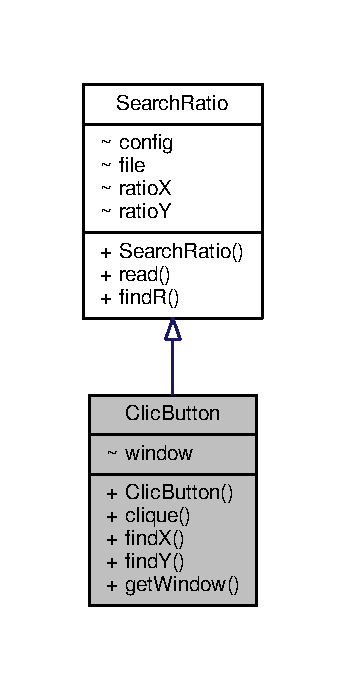
\includegraphics[width=166pt]{classClicButton__inherit__graph}
\end{center}
\end{figure}


Graphe de collaboration de Clic\+Button\+:\nopagebreak
\begin{figure}[H]
\begin{center}
\leavevmode
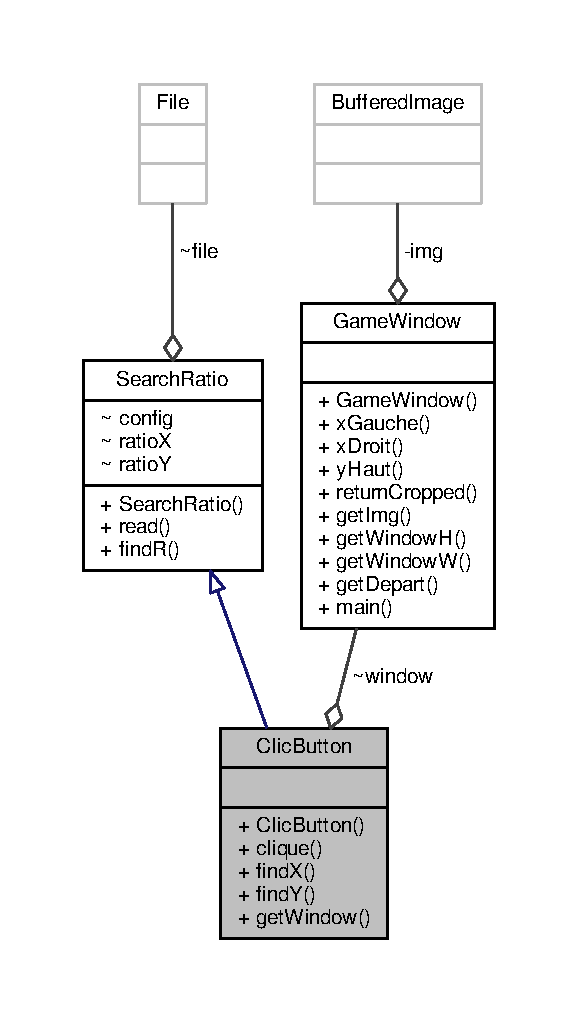
\includegraphics[width=278pt]{classClicButton__coll__graph}
\end{center}
\end{figure}
\subsubsection*{Fonctions membres publiques}
\begin{DoxyCompactItemize}
\item 
\hyperlink{classClicButton_a836009909fefe19c4c9232d5e8e9c926}{Clic\+Button} (File \hyperlink{classSearchRatio_a06393eaf84ff3e3f8c7f48e91b0b5e6a}{file})
\item 
void \hyperlink{classClicButton_ae6aa14adab27c29bff260ca38698f080}{clique} (String s)
\item 
int \hyperlink{classClicButton_ad41856b68437ce1373daac34f28161b6}{find\+X} (double ratio)
\item 
int \hyperlink{classClicButton_a838800b9bf1a7c4f7aed638c3401c3e0}{find\+Y} (double ratio)
\item 
\hyperlink{classGameWindow}{Game\+Window} \hyperlink{classClicButton_abeb3ae6fad1eccc494352fea4c34cd57}{get\+Window} ()
\item 
void \hyperlink{classSearchRatio_a03de53bdc48b4718858ef22d1ada2abd}{read} ()
\item 
void \hyperlink{classSearchRatio_a7c19f67d1f2ef6275d1a84bfdd3b2112}{find\+R} (String s)
\end{DoxyCompactItemize}
\subsubsection*{Attributs de paquetage}
\begin{DoxyCompactItemize}
\item 
\hyperlink{classGameWindow}{Game\+Window} \hyperlink{classClicButton_a0ed15aa9c93ab63c83289b0ce3202bd0}{window}
\item 
String \hyperlink{classSearchRatio_a5d7639c24edb76bea0854c5b5346bc18}{config}
\item 
File \hyperlink{classSearchRatio_a06393eaf84ff3e3f8c7f48e91b0b5e6a}{file}
\item 
double \hyperlink{classSearchRatio_a0310652e5c5da25ebb2eeabe4f90308a}{ratio\+X}
\item 
double \hyperlink{classSearchRatio_a0c0087388c099310eee409fb48bcef00}{ratio\+Y}
\end{DoxyCompactItemize}


\subsubsection{Documentation des constructeurs et destructeur}
\hypertarget{classClicButton_a836009909fefe19c4c9232d5e8e9c926}{}\index{Clic\+Button@{Clic\+Button}!Clic\+Button@{Clic\+Button}}
\index{Clic\+Button@{Clic\+Button}!Clic\+Button@{Clic\+Button}}
\paragraph[{Clic\+Button}]{\setlength{\rightskip}{0pt plus 5cm}Clic\+Button.\+Clic\+Button (
\begin{DoxyParamCaption}
\item[{File}]{file}
\end{DoxyParamCaption}
)}\label{classClicButton_a836009909fefe19c4c9232d5e8e9c926}


\subsubsection{Documentation des fonctions membres}
\hypertarget{classClicButton_ae6aa14adab27c29bff260ca38698f080}{}\index{Clic\+Button@{Clic\+Button}!clique@{clique}}
\index{clique@{clique}!Clic\+Button@{Clic\+Button}}
\paragraph[{clique}]{\setlength{\rightskip}{0pt plus 5cm}void Clic\+Button.\+clique (
\begin{DoxyParamCaption}
\item[{String}]{s}
\end{DoxyParamCaption}
)}\label{classClicButton_ae6aa14adab27c29bff260ca38698f080}


Référencé par Game\+Window.\+main().

\hypertarget{classSearchRatio_a7c19f67d1f2ef6275d1a84bfdd3b2112}{}\index{Clic\+Button@{Clic\+Button}!find\+R@{find\+R}}
\index{find\+R@{find\+R}!Clic\+Button@{Clic\+Button}}
\paragraph[{find\+R}]{\setlength{\rightskip}{0pt plus 5cm}void Search\+Ratio.\+find\+R (
\begin{DoxyParamCaption}
\item[{String}]{s}
\end{DoxyParamCaption}
)\hspace{0.3cm}{\ttfamily [inherited]}}\label{classSearchRatio_a7c19f67d1f2ef6275d1a84bfdd3b2112}


Référencé par clique().

\hypertarget{classClicButton_ad41856b68437ce1373daac34f28161b6}{}\index{Clic\+Button@{Clic\+Button}!find\+X@{find\+X}}
\index{find\+X@{find\+X}!Clic\+Button@{Clic\+Button}}
\paragraph[{find\+X}]{\setlength{\rightskip}{0pt plus 5cm}int Clic\+Button.\+find\+X (
\begin{DoxyParamCaption}
\item[{double}]{ratio}
\end{DoxyParamCaption}
)}\label{classClicButton_ad41856b68437ce1373daac34f28161b6}
\hypertarget{classClicButton_a838800b9bf1a7c4f7aed638c3401c3e0}{}\index{Clic\+Button@{Clic\+Button}!find\+Y@{find\+Y}}
\index{find\+Y@{find\+Y}!Clic\+Button@{Clic\+Button}}
\paragraph[{find\+Y}]{\setlength{\rightskip}{0pt plus 5cm}int Clic\+Button.\+find\+Y (
\begin{DoxyParamCaption}
\item[{double}]{ratio}
\end{DoxyParamCaption}
)}\label{classClicButton_a838800b9bf1a7c4f7aed638c3401c3e0}
\hypertarget{classClicButton_abeb3ae6fad1eccc494352fea4c34cd57}{}\index{Clic\+Button@{Clic\+Button}!get\+Window@{get\+Window}}
\index{get\+Window@{get\+Window}!Clic\+Button@{Clic\+Button}}
\paragraph[{get\+Window}]{\setlength{\rightskip}{0pt plus 5cm}{\bf Game\+Window} Clic\+Button.\+get\+Window (
\begin{DoxyParamCaption}
{}
\end{DoxyParamCaption}
)}\label{classClicButton_abeb3ae6fad1eccc494352fea4c34cd57}
\hypertarget{classSearchRatio_a03de53bdc48b4718858ef22d1ada2abd}{}\index{Clic\+Button@{Clic\+Button}!read@{read}}
\index{read@{read}!Clic\+Button@{Clic\+Button}}
\paragraph[{read}]{\setlength{\rightskip}{0pt plus 5cm}void Search\+Ratio.\+read (
\begin{DoxyParamCaption}
{}
\end{DoxyParamCaption}
)\hspace{0.3cm}{\ttfamily [inherited]}}\label{classSearchRatio_a03de53bdc48b4718858ef22d1ada2abd}


Référencé par Search\+Ratio.\+Search\+Ratio().



\subsubsection{Documentation des données membres}
\hypertarget{classSearchRatio_a5d7639c24edb76bea0854c5b5346bc18}{}\index{Clic\+Button@{Clic\+Button}!config@{config}}
\index{config@{config}!Clic\+Button@{Clic\+Button}}
\paragraph[{config}]{\setlength{\rightskip}{0pt plus 5cm}String Search\+Ratio.\+config\hspace{0.3cm}{\ttfamily [package]}, {\ttfamily [inherited]}}\label{classSearchRatio_a5d7639c24edb76bea0854c5b5346bc18}
\hypertarget{classSearchRatio_a06393eaf84ff3e3f8c7f48e91b0b5e6a}{}\index{Clic\+Button@{Clic\+Button}!file@{file}}
\index{file@{file}!Clic\+Button@{Clic\+Button}}
\paragraph[{file}]{\setlength{\rightskip}{0pt plus 5cm}File Search\+Ratio.\+file\hspace{0.3cm}{\ttfamily [package]}, {\ttfamily [inherited]}}\label{classSearchRatio_a06393eaf84ff3e3f8c7f48e91b0b5e6a}


Référencé par Search\+Ratio.\+Search\+Ratio().

\hypertarget{classSearchRatio_a0310652e5c5da25ebb2eeabe4f90308a}{}\index{Clic\+Button@{Clic\+Button}!ratio\+X@{ratio\+X}}
\index{ratio\+X@{ratio\+X}!Clic\+Button@{Clic\+Button}}
\paragraph[{ratio\+X}]{\setlength{\rightskip}{0pt plus 5cm}double Search\+Ratio.\+ratio\+X\hspace{0.3cm}{\ttfamily [package]}, {\ttfamily [inherited]}}\label{classSearchRatio_a0310652e5c5da25ebb2eeabe4f90308a}


Référencé par clique().

\hypertarget{classSearchRatio_a0c0087388c099310eee409fb48bcef00}{}\index{Clic\+Button@{Clic\+Button}!ratio\+Y@{ratio\+Y}}
\index{ratio\+Y@{ratio\+Y}!Clic\+Button@{Clic\+Button}}
\paragraph[{ratio\+Y}]{\setlength{\rightskip}{0pt plus 5cm}double Search\+Ratio.\+ratio\+Y\hspace{0.3cm}{\ttfamily [package]}, {\ttfamily [inherited]}}\label{classSearchRatio_a0c0087388c099310eee409fb48bcef00}


Référencé par clique().

\hypertarget{classClicButton_a0ed15aa9c93ab63c83289b0ce3202bd0}{}\index{Clic\+Button@{Clic\+Button}!window@{window}}
\index{window@{window}!Clic\+Button@{Clic\+Button}}
\paragraph[{window}]{\setlength{\rightskip}{0pt plus 5cm}{\bf Game\+Window} Clic\+Button.\+window\hspace{0.3cm}{\ttfamily [package]}}\label{classClicButton_a0ed15aa9c93ab63c83289b0ce3202bd0}


Référencé par get\+Window().



La documentation de cette classe a été générée à partir du fichier suivant \+:\begin{DoxyCompactItemize}
\item 
\hyperlink{ClicButton_8java}{Clic\+Button.\+java}\end{DoxyCompactItemize}

\hypertarget{classSuchi_1_1Client}{}\subsection{Référence de la classe Suchi.\+Client}
\label{classSuchi_1_1Client}\index{Suchi.\+Client@{Suchi.\+Client}}


Graphe de collaboration de Suchi.\+Client\+:\nopagebreak
\begin{figure}[H]
\begin{center}
\leavevmode
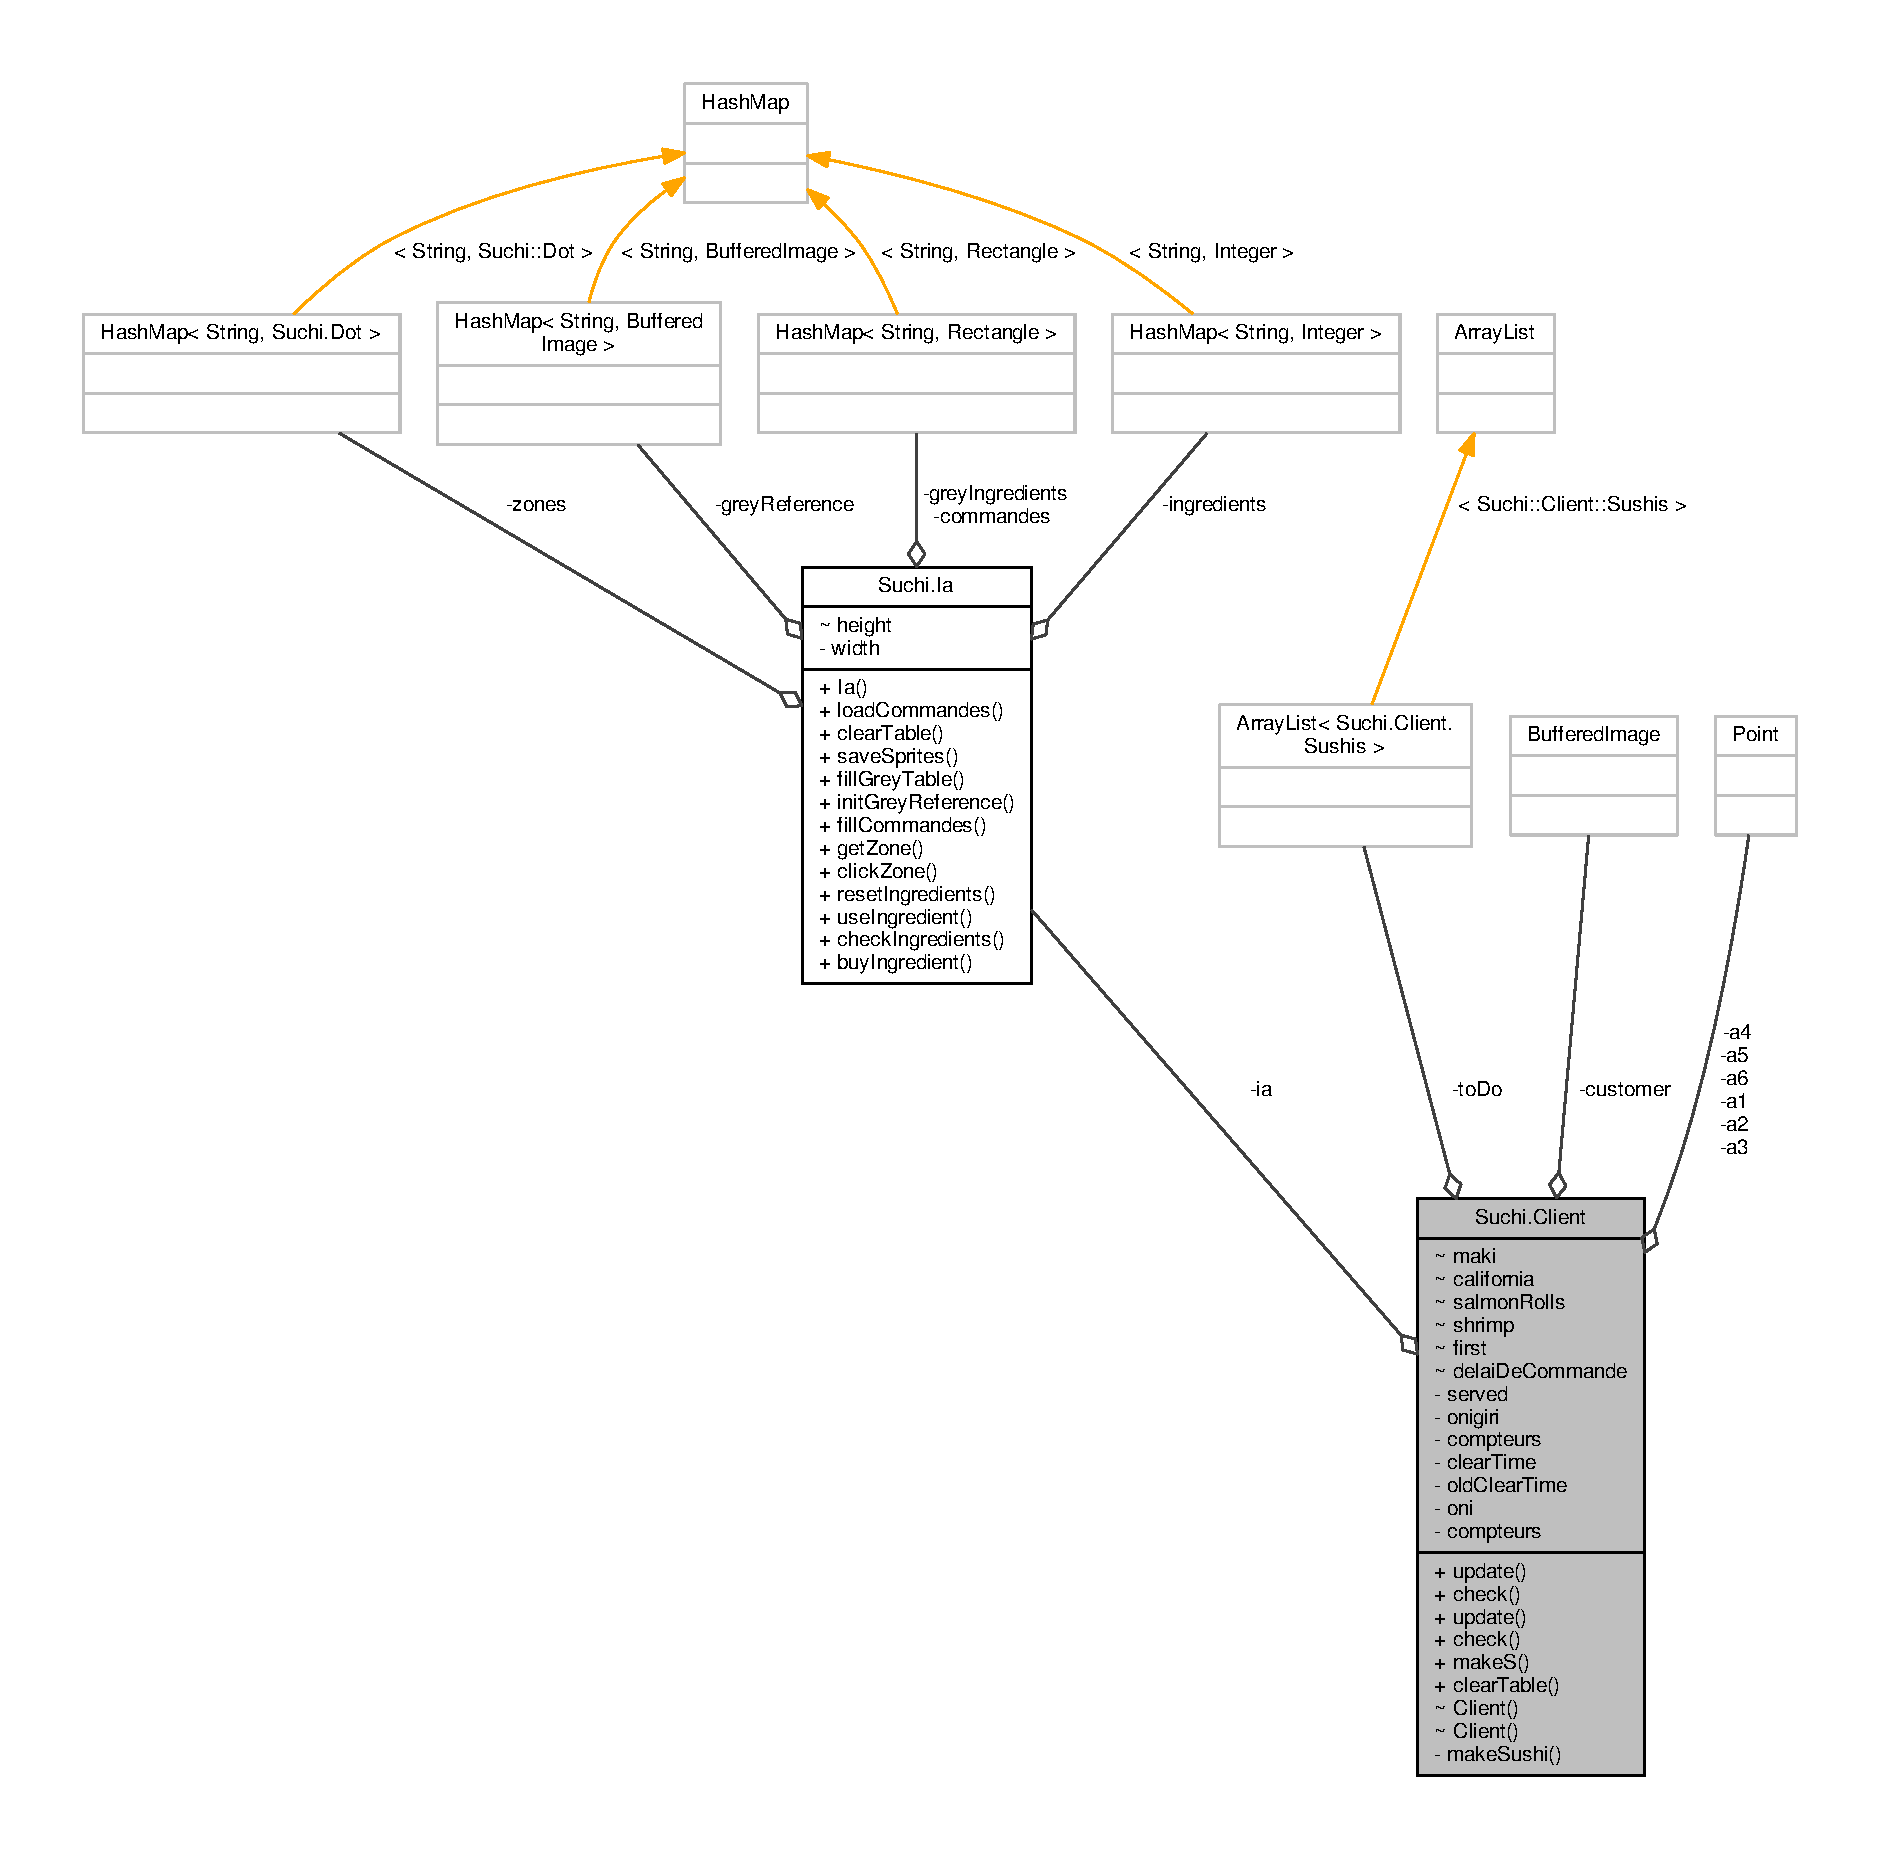
\includegraphics[width=350pt]{classSuchi_1_1Client__coll__graph}
\end{center}
\end{figure}
\subsubsection*{Classes}
\begin{DoxyCompactItemize}
\item 
enum \hyperlink{enumSuchi_1_1Client_1_1Sushis}{Sushis}
\end{DoxyCompactItemize}
\subsubsection*{Fonctions membres publiques}
\begin{DoxyCompactItemize}
\item 
void \hyperlink{classSuchi_1_1Client_a25f9c46121283d370fcfa8ecdfb32da1}{update} ()  throws Headless\+Exception, A\+W\+T\+Exception
\begin{DoxyCompactList}\small\item\em La méthode update est appellé en permanence et permet de détecter les nouvelles commandes. \end{DoxyCompactList}\item 
void \hyperlink{classSuchi_1_1Client_a533b9a4a8b34bc7915cc8c23e92d902b}{check} ()  throws Exception
\item 
void \hyperlink{classSuchi_1_1Client_a25f9c46121283d370fcfa8ecdfb32da1}{update} ()  throws Headless\+Exception, A\+W\+T\+Exception
\item 
void \hyperlink{classSuchi_1_1Client_a533b9a4a8b34bc7915cc8c23e92d902b}{check} ()  throws A\+W\+T\+Exception, Interrupted\+Exception
\item 
void \hyperlink{classSuchi_1_1Client_a9ac10e872438c578a9c9ec5f004710a5}{make\+S} ()  throws A\+W\+T\+Exception, Interrupted\+Exception
\item 
void \hyperlink{classSuchi_1_1Client_a96162d3186686e4aaebe6412d449d09f}{clear\+Table} ()  throws A\+W\+T\+Exception
\end{DoxyCompactItemize}
\subsubsection*{Fonctions de paquetage}
\begin{DoxyCompactItemize}
\item 
\hyperlink{classSuchi_1_1Client_a843ecec0eb9839c30568dab811b28485}{Client} ()  throws Exception
\begin{DoxyCompactList}\small\item\em Constructeur. \end{DoxyCompactList}\item 
\hyperlink{classSuchi_1_1Client_a843ecec0eb9839c30568dab811b28485}{Client} ()  throws Headless\+Exception, A\+W\+T\+Exception
\end{DoxyCompactItemize}
\subsubsection*{Attributs de paquetage}
\begin{DoxyCompactItemize}
\item 
String \hyperlink{classSuchi_1_1Client_ac4f46175dd37202e3e7bc24e30564766}{maki}
\item 
String \hyperlink{classSuchi_1_1Client_a2ac9fa1b6ec89770b63ffa9c23504657}{california}
\item 
String \hyperlink{classSuchi_1_1Client_a8724d79f7d9f7e2720ae6be2331475d4}{salmon\+Rolls}
\item 
String \hyperlink{classSuchi_1_1Client_af49dfab5d81b322967e58bc85aa2cd81}{shrimp}
\end{DoxyCompactItemize}
\subsubsection*{Attributs statiques de paquetage}
\begin{DoxyCompactItemize}
\item 
static Boolean \hyperlink{classSuchi_1_1Client_a49b4963073d8a2e5f27a4e28ef6a34b4}{first} = true
\item 
static int \hyperlink{classSuchi_1_1Client_a3c43b94040bc2b1368f63270b8dbeeaf}{delai\+De\+Commande} = 30000
\end{DoxyCompactItemize}
\subsubsection*{Fonctions membres privées}
\begin{DoxyCompactItemize}
\item 
void \hyperlink{classSuchi_1_1Client_aa9dfeaacdef8b8b3815e544e6b7217f8}{make\+Sushi} (String s)  throws Exception
\begin{DoxyCompactList}\small\item\em Méthode qui permet de créer le sushi demandé et mettre à jour les informations sur les quantités d\textquotesingle{}ingrédients. \end{DoxyCompactList}\end{DoxyCompactItemize}
\subsubsection*{Attributs privés}
\begin{DoxyCompactItemize}
\item 
Buffered\+Image\mbox{[}$\,$\mbox{]} \hyperlink{classSuchi_1_1Client_a046d048c1578b8d748d09e7efaaebb12}{customer}
\item 
boolean \hyperlink{classSuchi_1_1Client_a543ce771d09e264df72783f30bcb2a05}{served} \mbox{[}$\,$\mbox{]}
\item 
String \hyperlink{classSuchi_1_1Client_a0d8eba93c20ea516917b12db42233ea4}{onigiri}
\item 
long\mbox{[}$\,$\mbox{]} \hyperlink{classSuchi_1_1Client_a6f5dcd685fb0d9bede8b40feaf618ba2}{compteurs}
\item 
\hyperlink{classSuchi_1_1Ia}{Ia} \hyperlink{classSuchi_1_1Client_a1081e8917f8ab6e73a16188230466238}{ia}
\item 
long \hyperlink{classSuchi_1_1Client_acfd362a167b9e4d091ab44af7d0d1592}{clear\+Time} = 0
\item 
long \hyperlink{classSuchi_1_1Client_adb0ad87962ba3a22c4ab0c4553211606}{old\+Clear\+Time}
\item 
String \hyperlink{classSuchi_1_1Client_a934abfd3eaf4306d165bcbda8cc22ee0}{oni}
\item 
Array\+List$<$ \hyperlink{enumSuchi_1_1Client_1_1Sushis}{Sushis} $>$ \hyperlink{classSuchi_1_1Client_ad8f1efef85f217db94de5bfb30ff6a60}{to\+Do}
\item 
int\mbox{[}$\,$\mbox{]} \hyperlink{classSuchi_1_1Client_a8bdd5e9661c04f49b0709016a606b458}{compteurs}
\item 
final Point \hyperlink{classSuchi_1_1Client_a73039e1ad15b729f9432670b85e34b3b}{a1} = new Point (280,373)
\item 
final Point \hyperlink{classSuchi_1_1Client_a79d43b768d46513e88699479f8c990a3}{a2} = new Point (425,373)
\item 
final Point \hyperlink{classSuchi_1_1Client_a192135bbe1b59fd33d1bc0bdabc8037d}{a3} = new Point (578,373)
\item 
final Point \hyperlink{classSuchi_1_1Client_afcbd53977c80f31d0b75d8ff5a99ff6c}{a4} = new Point (729,373)
\item 
final Point \hyperlink{classSuchi_1_1Client_a7b43715a5440aafd01faa6816ab60ac4}{a5} = new Point (877,373)
\item 
final Point \hyperlink{classSuchi_1_1Client_ab2d3ab062091c7500b984738023c78b5}{a6} = new Point (1031,373)
\end{DoxyCompactItemize}


\subsubsection{Documentation des constructeurs et destructeur}
\hypertarget{classSuchi_1_1Client_a843ecec0eb9839c30568dab811b28485}{}\index{Suchi\+::\+Client@{Suchi\+::\+Client}!Client@{Client}}
\index{Client@{Client}!Suchi\+::\+Client@{Suchi\+::\+Client}}
\paragraph[{Client}]{\setlength{\rightskip}{0pt plus 5cm}Suchi.\+Client.\+Client (
\begin{DoxyParamCaption}
{}
\end{DoxyParamCaption}
) throws Exception\hspace{0.3cm}{\ttfamily [package]}}\label{classSuchi_1_1Client_a843ecec0eb9839c30568dab811b28485}


Constructeur. 


\begin{DoxyExceptions}{Exceptions}
{\em Exception} & \\
\hline
\end{DoxyExceptions}
\hypertarget{classSuchi_1_1Client_a843ecec0eb9839c30568dab811b28485}{}\index{Suchi\+::\+Client@{Suchi\+::\+Client}!Client@{Client}}
\index{Client@{Client}!Suchi\+::\+Client@{Suchi\+::\+Client}}
\paragraph[{Client}]{\setlength{\rightskip}{0pt plus 5cm}Suchi.\+Client.\+Client (
\begin{DoxyParamCaption}
{}
\end{DoxyParamCaption}
) throws Headless\+Exception, A\+W\+T\+Exception\hspace{0.3cm}{\ttfamily [package]}}\label{classSuchi_1_1Client_a843ecec0eb9839c30568dab811b28485}


\subsubsection{Documentation des fonctions membres}
\hypertarget{classSuchi_1_1Client_a533b9a4a8b34bc7915cc8c23e92d902b}{}\index{Suchi\+::\+Client@{Suchi\+::\+Client}!check@{check}}
\index{check@{check}!Suchi\+::\+Client@{Suchi\+::\+Client}}
\paragraph[{check}]{\setlength{\rightskip}{0pt plus 5cm}void Suchi.\+Client.\+check (
\begin{DoxyParamCaption}
{}
\end{DoxyParamCaption}
) throws A\+W\+T\+Exception, Interrupted\+Exception}\label{classSuchi_1_1Client_a533b9a4a8b34bc7915cc8c23e92d902b}
\hypertarget{classSuchi_1_1Client_a533b9a4a8b34bc7915cc8c23e92d902b}{}\index{Suchi\+::\+Client@{Suchi\+::\+Client}!check@{check}}
\index{check@{check}!Suchi\+::\+Client@{Suchi\+::\+Client}}
\paragraph[{check}]{\setlength{\rightskip}{0pt plus 5cm}void Suchi.\+Client.\+check (
\begin{DoxyParamCaption}
{}
\end{DoxyParamCaption}
) throws Exception}\label{classSuchi_1_1Client_a533b9a4a8b34bc7915cc8c23e92d902b}

\begin{DoxyExceptions}{Exceptions}
{\em Exception} & \\
\hline
\end{DoxyExceptions}


Référencé par Suchi.\+Game.\+main().

\hypertarget{classSuchi_1_1Client_a96162d3186686e4aaebe6412d449d09f}{}\index{Suchi\+::\+Client@{Suchi\+::\+Client}!clear\+Table@{clear\+Table}}
\index{clear\+Table@{clear\+Table}!Suchi\+::\+Client@{Suchi\+::\+Client}}
\paragraph[{clear\+Table}]{\setlength{\rightskip}{0pt plus 5cm}void Suchi.\+Client.\+clear\+Table (
\begin{DoxyParamCaption}
{}
\end{DoxyParamCaption}
) throws A\+W\+T\+Exception}\label{classSuchi_1_1Client_a96162d3186686e4aaebe6412d449d09f}


Référencé par Suchi.\+Client.\+check().

\hypertarget{classSuchi_1_1Client_a9ac10e872438c578a9c9ec5f004710a5}{}\index{Suchi\+::\+Client@{Suchi\+::\+Client}!make\+S@{make\+S}}
\index{make\+S@{make\+S}!Suchi\+::\+Client@{Suchi\+::\+Client}}
\paragraph[{make\+S}]{\setlength{\rightskip}{0pt plus 5cm}void Suchi.\+Client.\+make\+S (
\begin{DoxyParamCaption}
{}
\end{DoxyParamCaption}
) throws A\+W\+T\+Exception, Interrupted\+Exception}\label{classSuchi_1_1Client_a9ac10e872438c578a9c9ec5f004710a5}


Référencé par Suchi.\+Client.\+check().

\hypertarget{classSuchi_1_1Client_aa9dfeaacdef8b8b3815e544e6b7217f8}{}\index{Suchi\+::\+Client@{Suchi\+::\+Client}!make\+Sushi@{make\+Sushi}}
\index{make\+Sushi@{make\+Sushi}!Suchi\+::\+Client@{Suchi\+::\+Client}}
\paragraph[{make\+Sushi}]{\setlength{\rightskip}{0pt plus 5cm}void Suchi.\+Client.\+make\+Sushi (
\begin{DoxyParamCaption}
\item[{String}]{s}
\end{DoxyParamCaption}
) throws Exception\hspace{0.3cm}{\ttfamily [private]}}\label{classSuchi_1_1Client_aa9dfeaacdef8b8b3815e544e6b7217f8}


Méthode qui permet de créer le sushi demandé et mettre à jour les informations sur les quantités d\textquotesingle{}ingrédients. 


\begin{DoxyParams}{Paramètres}
{\em s} & String le sushi à réaliser \\
\hline
\end{DoxyParams}

\begin{DoxyExceptions}{Exceptions}
{\em Exception} & \\
\hline
\end{DoxyExceptions}


Référencé par Suchi.\+Client.\+check().

\hypertarget{classSuchi_1_1Client_a25f9c46121283d370fcfa8ecdfb32da1}{}\index{Suchi\+::\+Client@{Suchi\+::\+Client}!update@{update}}
\index{update@{update}!Suchi\+::\+Client@{Suchi\+::\+Client}}
\paragraph[{update}]{\setlength{\rightskip}{0pt plus 5cm}void Suchi.\+Client.\+update (
\begin{DoxyParamCaption}
{}
\end{DoxyParamCaption}
) throws Headless\+Exception, A\+W\+T\+Exception}\label{classSuchi_1_1Client_a25f9c46121283d370fcfa8ecdfb32da1}
\hypertarget{classSuchi_1_1Client_a25f9c46121283d370fcfa8ecdfb32da1}{}\index{Suchi\+::\+Client@{Suchi\+::\+Client}!update@{update}}
\index{update@{update}!Suchi\+::\+Client@{Suchi\+::\+Client}}
\paragraph[{update}]{\setlength{\rightskip}{0pt plus 5cm}void Suchi.\+Client.\+update (
\begin{DoxyParamCaption}
{}
\end{DoxyParamCaption}
) throws Headless\+Exception, A\+W\+T\+Exception}\label{classSuchi_1_1Client_a25f9c46121283d370fcfa8ecdfb32da1}


La méthode update est appellé en permanence et permet de détecter les nouvelles commandes. 


\begin{DoxyExceptions}{Exceptions}
{\em Headless\+Exception} & \\
\hline
{\em A\+W\+T\+Exception} & \\
\hline
\end{DoxyExceptions}


Référencé par Suchi.\+Game.\+main().



\subsubsection{Documentation des données membres}
\hypertarget{classSuchi_1_1Client_a73039e1ad15b729f9432670b85e34b3b}{}\index{Suchi\+::\+Client@{Suchi\+::\+Client}!a1@{a1}}
\index{a1@{a1}!Suchi\+::\+Client@{Suchi\+::\+Client}}
\paragraph[{a1}]{\setlength{\rightskip}{0pt plus 5cm}final Point Suchi.\+Client.\+a1 = new Point (280,373)\hspace{0.3cm}{\ttfamily [private]}}\label{classSuchi_1_1Client_a73039e1ad15b729f9432670b85e34b3b}
\hypertarget{classSuchi_1_1Client_a79d43b768d46513e88699479f8c990a3}{}\index{Suchi\+::\+Client@{Suchi\+::\+Client}!a2@{a2}}
\index{a2@{a2}!Suchi\+::\+Client@{Suchi\+::\+Client}}
\paragraph[{a2}]{\setlength{\rightskip}{0pt plus 5cm}final Point Suchi.\+Client.\+a2 = new Point (425,373)\hspace{0.3cm}{\ttfamily [private]}}\label{classSuchi_1_1Client_a79d43b768d46513e88699479f8c990a3}
\hypertarget{classSuchi_1_1Client_a192135bbe1b59fd33d1bc0bdabc8037d}{}\index{Suchi\+::\+Client@{Suchi\+::\+Client}!a3@{a3}}
\index{a3@{a3}!Suchi\+::\+Client@{Suchi\+::\+Client}}
\paragraph[{a3}]{\setlength{\rightskip}{0pt plus 5cm}final Point Suchi.\+Client.\+a3 = new Point (578,373)\hspace{0.3cm}{\ttfamily [private]}}\label{classSuchi_1_1Client_a192135bbe1b59fd33d1bc0bdabc8037d}
\hypertarget{classSuchi_1_1Client_afcbd53977c80f31d0b75d8ff5a99ff6c}{}\index{Suchi\+::\+Client@{Suchi\+::\+Client}!a4@{a4}}
\index{a4@{a4}!Suchi\+::\+Client@{Suchi\+::\+Client}}
\paragraph[{a4}]{\setlength{\rightskip}{0pt plus 5cm}final Point Suchi.\+Client.\+a4 = new Point (729,373)\hspace{0.3cm}{\ttfamily [private]}}\label{classSuchi_1_1Client_afcbd53977c80f31d0b75d8ff5a99ff6c}
\hypertarget{classSuchi_1_1Client_a7b43715a5440aafd01faa6816ab60ac4}{}\index{Suchi\+::\+Client@{Suchi\+::\+Client}!a5@{a5}}
\index{a5@{a5}!Suchi\+::\+Client@{Suchi\+::\+Client}}
\paragraph[{a5}]{\setlength{\rightskip}{0pt plus 5cm}final Point Suchi.\+Client.\+a5 = new Point (877,373)\hspace{0.3cm}{\ttfamily [private]}}\label{classSuchi_1_1Client_a7b43715a5440aafd01faa6816ab60ac4}
\hypertarget{classSuchi_1_1Client_ab2d3ab062091c7500b984738023c78b5}{}\index{Suchi\+::\+Client@{Suchi\+::\+Client}!a6@{a6}}
\index{a6@{a6}!Suchi\+::\+Client@{Suchi\+::\+Client}}
\paragraph[{a6}]{\setlength{\rightskip}{0pt plus 5cm}final Point Suchi.\+Client.\+a6 = new Point (1031,373)\hspace{0.3cm}{\ttfamily [private]}}\label{classSuchi_1_1Client_ab2d3ab062091c7500b984738023c78b5}
\hypertarget{classSuchi_1_1Client_a2ac9fa1b6ec89770b63ffa9c23504657}{}\index{Suchi\+::\+Client@{Suchi\+::\+Client}!california@{california}}
\index{california@{california}!Suchi\+::\+Client@{Suchi\+::\+Client}}
\paragraph[{california}]{\setlength{\rightskip}{0pt plus 5cm}String Suchi.\+Client.\+california\hspace{0.3cm}{\ttfamily [package]}}\label{classSuchi_1_1Client_a2ac9fa1b6ec89770b63ffa9c23504657}
\hypertarget{classSuchi_1_1Client_acfd362a167b9e4d091ab44af7d0d1592}{}\index{Suchi\+::\+Client@{Suchi\+::\+Client}!clear\+Time@{clear\+Time}}
\index{clear\+Time@{clear\+Time}!Suchi\+::\+Client@{Suchi\+::\+Client}}
\paragraph[{clear\+Time}]{\setlength{\rightskip}{0pt plus 5cm}long Suchi.\+Client.\+clear\+Time = 0\hspace{0.3cm}{\ttfamily [private]}}\label{classSuchi_1_1Client_acfd362a167b9e4d091ab44af7d0d1592}


Référencé par Suchi.\+Client.\+check().

\hypertarget{classSuchi_1_1Client_a6f5dcd685fb0d9bede8b40feaf618ba2}{}\index{Suchi\+::\+Client@{Suchi\+::\+Client}!compteurs@{compteurs}}
\index{compteurs@{compteurs}!Suchi\+::\+Client@{Suchi\+::\+Client}}
\paragraph[{compteurs}]{\setlength{\rightskip}{0pt plus 5cm}long \mbox{[}$\,$\mbox{]} Suchi.\+Client.\+compteurs\hspace{0.3cm}{\ttfamily [private]}}\label{classSuchi_1_1Client_a6f5dcd685fb0d9bede8b40feaf618ba2}
\hypertarget{classSuchi_1_1Client_a8bdd5e9661c04f49b0709016a606b458}{}\index{Suchi\+::\+Client@{Suchi\+::\+Client}!compteurs@{compteurs}}
\index{compteurs@{compteurs}!Suchi\+::\+Client@{Suchi\+::\+Client}}
\paragraph[{compteurs}]{\setlength{\rightskip}{0pt plus 5cm}int \mbox{[}$\,$\mbox{]} Suchi.\+Client.\+compteurs\hspace{0.3cm}{\ttfamily [private]}}\label{classSuchi_1_1Client_a8bdd5e9661c04f49b0709016a606b458}
\hypertarget{classSuchi_1_1Client_a046d048c1578b8d748d09e7efaaebb12}{}\index{Suchi\+::\+Client@{Suchi\+::\+Client}!customer@{customer}}
\index{customer@{customer}!Suchi\+::\+Client@{Suchi\+::\+Client}}
\paragraph[{customer}]{\setlength{\rightskip}{0pt plus 5cm}Buffered\+Image \mbox{[}$\,$\mbox{]} Suchi.\+Client.\+customer\hspace{0.3cm}{\ttfamily [private]}}\label{classSuchi_1_1Client_a046d048c1578b8d748d09e7efaaebb12}
\hypertarget{classSuchi_1_1Client_a3c43b94040bc2b1368f63270b8dbeeaf}{}\index{Suchi\+::\+Client@{Suchi\+::\+Client}!delai\+De\+Commande@{delai\+De\+Commande}}
\index{delai\+De\+Commande@{delai\+De\+Commande}!Suchi\+::\+Client@{Suchi\+::\+Client}}
\paragraph[{delai\+De\+Commande}]{\setlength{\rightskip}{0pt plus 5cm}int Suchi.\+Client.\+delai\+De\+Commande = 30000\hspace{0.3cm}{\ttfamily [static]}, {\ttfamily [package]}}\label{classSuchi_1_1Client_a3c43b94040bc2b1368f63270b8dbeeaf}
\hypertarget{classSuchi_1_1Client_a49b4963073d8a2e5f27a4e28ef6a34b4}{}\index{Suchi\+::\+Client@{Suchi\+::\+Client}!first@{first}}
\index{first@{first}!Suchi\+::\+Client@{Suchi\+::\+Client}}
\paragraph[{first}]{\setlength{\rightskip}{0pt plus 5cm}Boolean Suchi.\+Client.\+first = true\hspace{0.3cm}{\ttfamily [static]}, {\ttfamily [package]}}\label{classSuchi_1_1Client_a49b4963073d8a2e5f27a4e28ef6a34b4}
\hypertarget{classSuchi_1_1Client_a1081e8917f8ab6e73a16188230466238}{}\index{Suchi\+::\+Client@{Suchi\+::\+Client}!ia@{ia}}
\index{ia@{ia}!Suchi\+::\+Client@{Suchi\+::\+Client}}
\paragraph[{ia}]{\setlength{\rightskip}{0pt plus 5cm}{\bf Ia} Suchi.\+Client.\+ia\hspace{0.3cm}{\ttfamily [private]}}\label{classSuchi_1_1Client_a1081e8917f8ab6e73a16188230466238}
\hypertarget{classSuchi_1_1Client_ac4f46175dd37202e3e7bc24e30564766}{}\index{Suchi\+::\+Client@{Suchi\+::\+Client}!maki@{maki}}
\index{maki@{maki}!Suchi\+::\+Client@{Suchi\+::\+Client}}
\paragraph[{maki}]{\setlength{\rightskip}{0pt plus 5cm}String Suchi.\+Client.\+maki\hspace{0.3cm}{\ttfamily [package]}}\label{classSuchi_1_1Client_ac4f46175dd37202e3e7bc24e30564766}
\hypertarget{classSuchi_1_1Client_adb0ad87962ba3a22c4ab0c4553211606}{}\index{Suchi\+::\+Client@{Suchi\+::\+Client}!old\+Clear\+Time@{old\+Clear\+Time}}
\index{old\+Clear\+Time@{old\+Clear\+Time}!Suchi\+::\+Client@{Suchi\+::\+Client}}
\paragraph[{old\+Clear\+Time}]{\setlength{\rightskip}{0pt plus 5cm}long Suchi.\+Client.\+old\+Clear\+Time\hspace{0.3cm}{\ttfamily [private]}}\label{classSuchi_1_1Client_adb0ad87962ba3a22c4ab0c4553211606}
\hypertarget{classSuchi_1_1Client_a934abfd3eaf4306d165bcbda8cc22ee0}{}\index{Suchi\+::\+Client@{Suchi\+::\+Client}!oni@{oni}}
\index{oni@{oni}!Suchi\+::\+Client@{Suchi\+::\+Client}}
\paragraph[{oni}]{\setlength{\rightskip}{0pt plus 5cm}String Suchi.\+Client.\+oni\hspace{0.3cm}{\ttfamily [private]}}\label{classSuchi_1_1Client_a934abfd3eaf4306d165bcbda8cc22ee0}
\hypertarget{classSuchi_1_1Client_a0d8eba93c20ea516917b12db42233ea4}{}\index{Suchi\+::\+Client@{Suchi\+::\+Client}!onigiri@{onigiri}}
\index{onigiri@{onigiri}!Suchi\+::\+Client@{Suchi\+::\+Client}}
\paragraph[{onigiri}]{\setlength{\rightskip}{0pt plus 5cm}String Suchi.\+Client.\+onigiri\hspace{0.3cm}{\ttfamily [private]}}\label{classSuchi_1_1Client_a0d8eba93c20ea516917b12db42233ea4}
\hypertarget{classSuchi_1_1Client_a8724d79f7d9f7e2720ae6be2331475d4}{}\index{Suchi\+::\+Client@{Suchi\+::\+Client}!salmon\+Rolls@{salmon\+Rolls}}
\index{salmon\+Rolls@{salmon\+Rolls}!Suchi\+::\+Client@{Suchi\+::\+Client}}
\paragraph[{salmon\+Rolls}]{\setlength{\rightskip}{0pt plus 5cm}String Suchi.\+Client.\+salmon\+Rolls\hspace{0.3cm}{\ttfamily [package]}}\label{classSuchi_1_1Client_a8724d79f7d9f7e2720ae6be2331475d4}
\hypertarget{classSuchi_1_1Client_a543ce771d09e264df72783f30bcb2a05}{}\index{Suchi\+::\+Client@{Suchi\+::\+Client}!served@{served}}
\index{served@{served}!Suchi\+::\+Client@{Suchi\+::\+Client}}
\paragraph[{served}]{\setlength{\rightskip}{0pt plus 5cm}boolean Suchi.\+Client.\+served\hspace{0.3cm}{\ttfamily [private]}}\label{classSuchi_1_1Client_a543ce771d09e264df72783f30bcb2a05}
\hypertarget{classSuchi_1_1Client_af49dfab5d81b322967e58bc85aa2cd81}{}\index{Suchi\+::\+Client@{Suchi\+::\+Client}!shrimp@{shrimp}}
\index{shrimp@{shrimp}!Suchi\+::\+Client@{Suchi\+::\+Client}}
\paragraph[{shrimp}]{\setlength{\rightskip}{0pt plus 5cm}String Suchi.\+Client.\+shrimp\hspace{0.3cm}{\ttfamily [package]}}\label{classSuchi_1_1Client_af49dfab5d81b322967e58bc85aa2cd81}
\hypertarget{classSuchi_1_1Client_ad8f1efef85f217db94de5bfb30ff6a60}{}\index{Suchi\+::\+Client@{Suchi\+::\+Client}!to\+Do@{to\+Do}}
\index{to\+Do@{to\+Do}!Suchi\+::\+Client@{Suchi\+::\+Client}}
\paragraph[{to\+Do}]{\setlength{\rightskip}{0pt plus 5cm}Array\+List$<${\bf Sushis}$>$ Suchi.\+Client.\+to\+Do\hspace{0.3cm}{\ttfamily [private]}}\label{classSuchi_1_1Client_ad8f1efef85f217db94de5bfb30ff6a60}


La documentation de cette classe a été générée à partir du fichier suivant \+:\begin{DoxyCompactItemize}
\item 
\hyperlink{BotSofRetapage_2src_2Suchi_2Client_8java}{Bot\+Sof\+Retapage/src/\+Suchi/\+Client.\+java}\end{DoxyCompactItemize}

\hypertarget{classTestSushi_1_1src_1_1Suchi_1_1Client}{}\subsection{Référence de la classe Test\+Sushi.\+src.\+Suchi.\+Client}
\label{classTestSushi_1_1src_1_1Suchi_1_1Client}\index{Test\+Sushi.\+src.\+Suchi.\+Client@{Test\+Sushi.\+src.\+Suchi.\+Client}}


Graphe de collaboration de Test\+Sushi.\+src.\+Suchi.\+Client\+:\nopagebreak
\begin{figure}[H]
\begin{center}
\leavevmode
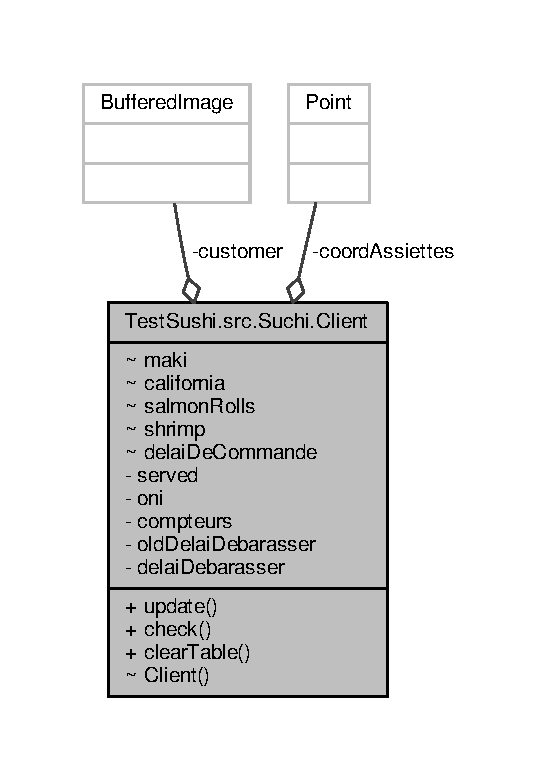
\includegraphics[width=259pt]{classTestSushi_1_1src_1_1Suchi_1_1Client__coll__graph}
\end{center}
\end{figure}
\subsubsection*{Classes}
\begin{DoxyCompactItemize}
\item 
enum \hyperlink{enumTestSushi_1_1src_1_1Suchi_1_1Client_1_1Sushis}{Sushis}
\end{DoxyCompactItemize}
\subsubsection*{Fonctions membres publiques}
\begin{DoxyCompactItemize}
\item 
void \hyperlink{classTestSushi_1_1src_1_1Suchi_1_1Client_a50f1e325b703b85c56546ca5999abeeb}{update} ()  throws Headless\+Exception, A\+W\+T\+Exception
\begin{DoxyCompactList}\small\item\em Méthode qui met à jour les captures d\textquotesingle{}écran de bulles des clients. \end{DoxyCompactList}\item 
void \hyperlink{classTestSushi_1_1src_1_1Suchi_1_1Client_ad353c24b9c2af3e11796d26050d88c48}{check} ()  throws A\+W\+T\+Exception, Interrupted\+Exception
\item 
void \hyperlink{classTestSushi_1_1src_1_1Suchi_1_1Client_af6f639320c7a31df600b0590487a1992}{clear\+Table} ()  throws A\+W\+T\+Exception 
\end{DoxyCompactItemize}
\subsubsection*{Fonctions de paquetage}
\begin{DoxyCompactItemize}
\item 
\hyperlink{classTestSushi_1_1src_1_1Suchi_1_1Client_aa526fb492301ef47dbaf7e0395416e60}{Client} ()  throws Headless\+Exception, A\+W\+T\+Exception
\begin{DoxyCompactList}\small\item\em Constructeur. \end{DoxyCompactList}\end{DoxyCompactItemize}
\subsubsection*{Attributs de paquetage}
\begin{DoxyCompactItemize}
\item 
String \hyperlink{classTestSushi_1_1src_1_1Suchi_1_1Client_a0de54dcf18e79e239fba1b01dece6ee5}{maki}
\item 
String \hyperlink{classTestSushi_1_1src_1_1Suchi_1_1Client_a2f0c0a782e724648db382a2de6abef73}{california}
\item 
String \hyperlink{classTestSushi_1_1src_1_1Suchi_1_1Client_aafc1efaa04206c67060116fe39c71371}{salmon\+Rolls}
\item 
String \hyperlink{classTestSushi_1_1src_1_1Suchi_1_1Client_ada365a5bc05af97839595dc0b04e5476}{shrimp}
\end{DoxyCompactItemize}
\subsubsection*{Attributs statiques de paquetage}
\begin{DoxyCompactItemize}
\item 
static int \hyperlink{classTestSushi_1_1src_1_1Suchi_1_1Client_a8e3568b2377a03a2c91e87ac6a978192}{delai\+De\+Commande} = 30000
\end{DoxyCompactItemize}
\subsubsection*{Attributs privés}
\begin{DoxyCompactItemize}
\item 
Buffered\+Image\mbox{[}$\,$\mbox{]} \hyperlink{classTestSushi_1_1src_1_1Suchi_1_1Client_a8344545c49813620c28454d4801437d0}{customer}
\item 
boolean \hyperlink{classTestSushi_1_1src_1_1Suchi_1_1Client_a488bd41ed3e3f10a8080f8fc39cea2bb}{served} \mbox{[}$\,$\mbox{]}
\item 
String \hyperlink{classTestSushi_1_1src_1_1Suchi_1_1Client_a03e30e98e66ce6aa2f6ccb6355924118}{oni}
\item 
long\mbox{[}$\,$\mbox{]} \hyperlink{classTestSushi_1_1src_1_1Suchi_1_1Client_a598d63640fd2871e55167937f9dcda68}{compteurs}
\item 
long \hyperlink{classTestSushi_1_1src_1_1Suchi_1_1Client_acbf22080fae7f82878cb444255a534fc}{old\+Delai\+Debarasser}
\item 
long \hyperlink{classTestSushi_1_1src_1_1Suchi_1_1Client_a6fb0a78e3afb6dea2b53216ccc0016bd}{delai\+Debarasser}
\item 
final Point\mbox{[}$\,$\mbox{]} \hyperlink{classTestSushi_1_1src_1_1Suchi_1_1Client_aef5b0a7a31e2789d55e78bbf997bec4c}{coord\+Assiettes}
\end{DoxyCompactItemize}


\subsubsection{Documentation des constructeurs et destructeur}
\hypertarget{classTestSushi_1_1src_1_1Suchi_1_1Client_aa526fb492301ef47dbaf7e0395416e60}{}\index{Test\+Sushi\+::src\+::\+Suchi\+::\+Client@{Test\+Sushi\+::src\+::\+Suchi\+::\+Client}!Client@{Client}}
\index{Client@{Client}!Test\+Sushi\+::src\+::\+Suchi\+::\+Client@{Test\+Sushi\+::src\+::\+Suchi\+::\+Client}}
\paragraph[{Client}]{\setlength{\rightskip}{0pt plus 5cm}Test\+Sushi.\+src.\+Suchi.\+Client.\+Client (
\begin{DoxyParamCaption}
{}
\end{DoxyParamCaption}
) throws Headless\+Exception, A\+W\+T\+Exception\hspace{0.3cm}{\ttfamily [package]}}\label{classTestSushi_1_1src_1_1Suchi_1_1Client_aa526fb492301ef47dbaf7e0395416e60}


Constructeur. 


\begin{DoxyExceptions}{Exceptions}
{\em Headless\+Exception} & \\
\hline
{\em A\+W\+T\+Exception} & \\
\hline
\end{DoxyExceptions}


\subsubsection{Documentation des fonctions membres}
\hypertarget{classTestSushi_1_1src_1_1Suchi_1_1Client_ad353c24b9c2af3e11796d26050d88c48}{}\index{Test\+Sushi\+::src\+::\+Suchi\+::\+Client@{Test\+Sushi\+::src\+::\+Suchi\+::\+Client}!check@{check}}
\index{check@{check}!Test\+Sushi\+::src\+::\+Suchi\+::\+Client@{Test\+Sushi\+::src\+::\+Suchi\+::\+Client}}
\paragraph[{check}]{\setlength{\rightskip}{0pt plus 5cm}void Test\+Sushi.\+src.\+Suchi.\+Client.\+check (
\begin{DoxyParamCaption}
{}
\end{DoxyParamCaption}
) throws A\+W\+T\+Exception, Interrupted\+Exception}\label{classTestSushi_1_1src_1_1Suchi_1_1Client_ad353c24b9c2af3e11796d26050d88c48}

\begin{DoxyExceptions}{Exceptions}
{\em A\+W\+T\+Exception} & \\
\hline
{\em Interrupted\+Exception} & \\
\hline
\end{DoxyExceptions}
\hypertarget{classTestSushi_1_1src_1_1Suchi_1_1Client_af6f639320c7a31df600b0590487a1992}{}\index{Test\+Sushi\+::src\+::\+Suchi\+::\+Client@{Test\+Sushi\+::src\+::\+Suchi\+::\+Client}!clear\+Table@{clear\+Table}}
\index{clear\+Table@{clear\+Table}!Test\+Sushi\+::src\+::\+Suchi\+::\+Client@{Test\+Sushi\+::src\+::\+Suchi\+::\+Client}}
\paragraph[{clear\+Table}]{\setlength{\rightskip}{0pt plus 5cm}void Test\+Sushi.\+src.\+Suchi.\+Client.\+clear\+Table (
\begin{DoxyParamCaption}
{}
\end{DoxyParamCaption}
) throws A\+W\+T\+Exception}\label{classTestSushi_1_1src_1_1Suchi_1_1Client_af6f639320c7a31df600b0590487a1992}


Référencé par Test\+Sushi.\+src.\+Suchi.\+Client.\+check().

\hypertarget{classTestSushi_1_1src_1_1Suchi_1_1Client_a50f1e325b703b85c56546ca5999abeeb}{}\index{Test\+Sushi\+::src\+::\+Suchi\+::\+Client@{Test\+Sushi\+::src\+::\+Suchi\+::\+Client}!update@{update}}
\index{update@{update}!Test\+Sushi\+::src\+::\+Suchi\+::\+Client@{Test\+Sushi\+::src\+::\+Suchi\+::\+Client}}
\paragraph[{update}]{\setlength{\rightskip}{0pt plus 5cm}void Test\+Sushi.\+src.\+Suchi.\+Client.\+update (
\begin{DoxyParamCaption}
{}
\end{DoxyParamCaption}
) throws Headless\+Exception, A\+W\+T\+Exception}\label{classTestSushi_1_1src_1_1Suchi_1_1Client_a50f1e325b703b85c56546ca5999abeeb}


Méthode qui met à jour les captures d\textquotesingle{}écran de bulles des clients. 


\begin{DoxyExceptions}{Exceptions}
{\em Headless\+Exception} & \\
\hline
{\em A\+W\+T\+Exception} & \\
\hline
\end{DoxyExceptions}


\subsubsection{Documentation des données membres}
\hypertarget{classTestSushi_1_1src_1_1Suchi_1_1Client_a2f0c0a782e724648db382a2de6abef73}{}\index{Test\+Sushi\+::src\+::\+Suchi\+::\+Client@{Test\+Sushi\+::src\+::\+Suchi\+::\+Client}!california@{california}}
\index{california@{california}!Test\+Sushi\+::src\+::\+Suchi\+::\+Client@{Test\+Sushi\+::src\+::\+Suchi\+::\+Client}}
\paragraph[{california}]{\setlength{\rightskip}{0pt plus 5cm}String Test\+Sushi.\+src.\+Suchi.\+Client.\+california\hspace{0.3cm}{\ttfamily [package]}}\label{classTestSushi_1_1src_1_1Suchi_1_1Client_a2f0c0a782e724648db382a2de6abef73}
\hypertarget{classTestSushi_1_1src_1_1Suchi_1_1Client_a598d63640fd2871e55167937f9dcda68}{}\index{Test\+Sushi\+::src\+::\+Suchi\+::\+Client@{Test\+Sushi\+::src\+::\+Suchi\+::\+Client}!compteurs@{compteurs}}
\index{compteurs@{compteurs}!Test\+Sushi\+::src\+::\+Suchi\+::\+Client@{Test\+Sushi\+::src\+::\+Suchi\+::\+Client}}
\paragraph[{compteurs}]{\setlength{\rightskip}{0pt plus 5cm}long \mbox{[}$\,$\mbox{]} Test\+Sushi.\+src.\+Suchi.\+Client.\+compteurs\hspace{0.3cm}{\ttfamily [private]}}\label{classTestSushi_1_1src_1_1Suchi_1_1Client_a598d63640fd2871e55167937f9dcda68}
\hypertarget{classTestSushi_1_1src_1_1Suchi_1_1Client_aef5b0a7a31e2789d55e78bbf997bec4c}{}\index{Test\+Sushi\+::src\+::\+Suchi\+::\+Client@{Test\+Sushi\+::src\+::\+Suchi\+::\+Client}!coord\+Assiettes@{coord\+Assiettes}}
\index{coord\+Assiettes@{coord\+Assiettes}!Test\+Sushi\+::src\+::\+Suchi\+::\+Client@{Test\+Sushi\+::src\+::\+Suchi\+::\+Client}}
\paragraph[{coord\+Assiettes}]{\setlength{\rightskip}{0pt plus 5cm}final Point \mbox{[}$\,$\mbox{]} Test\+Sushi.\+src.\+Suchi.\+Client.\+coord\+Assiettes\hspace{0.3cm}{\ttfamily [private]}}\label{classTestSushi_1_1src_1_1Suchi_1_1Client_aef5b0a7a31e2789d55e78bbf997bec4c}
{\bfseries Valeur initiale \+:}
\begin{DoxyCode}
= \textcolor{keyword}{new} Point[]\{
            \textcolor{keyword}{new} Point (280,373),
            \textcolor{keyword}{new} Point (425,373),
            \textcolor{keyword}{new} Point (578,373),
            \textcolor{keyword}{new} Point (729,373),
            \textcolor{keyword}{new} Point (877,373),
            \textcolor{keyword}{new} Point (1031,373)
    \}
\end{DoxyCode}
\hypertarget{classTestSushi_1_1src_1_1Suchi_1_1Client_a8344545c49813620c28454d4801437d0}{}\index{Test\+Sushi\+::src\+::\+Suchi\+::\+Client@{Test\+Sushi\+::src\+::\+Suchi\+::\+Client}!customer@{customer}}
\index{customer@{customer}!Test\+Sushi\+::src\+::\+Suchi\+::\+Client@{Test\+Sushi\+::src\+::\+Suchi\+::\+Client}}
\paragraph[{customer}]{\setlength{\rightskip}{0pt plus 5cm}Buffered\+Image \mbox{[}$\,$\mbox{]} Test\+Sushi.\+src.\+Suchi.\+Client.\+customer\hspace{0.3cm}{\ttfamily [private]}}\label{classTestSushi_1_1src_1_1Suchi_1_1Client_a8344545c49813620c28454d4801437d0}
\hypertarget{classTestSushi_1_1src_1_1Suchi_1_1Client_a6fb0a78e3afb6dea2b53216ccc0016bd}{}\index{Test\+Sushi\+::src\+::\+Suchi\+::\+Client@{Test\+Sushi\+::src\+::\+Suchi\+::\+Client}!delai\+Debarasser@{delai\+Debarasser}}
\index{delai\+Debarasser@{delai\+Debarasser}!Test\+Sushi\+::src\+::\+Suchi\+::\+Client@{Test\+Sushi\+::src\+::\+Suchi\+::\+Client}}
\paragraph[{delai\+Debarasser}]{\setlength{\rightskip}{0pt plus 5cm}long Test\+Sushi.\+src.\+Suchi.\+Client.\+delai\+Debarasser\hspace{0.3cm}{\ttfamily [private]}}\label{classTestSushi_1_1src_1_1Suchi_1_1Client_a6fb0a78e3afb6dea2b53216ccc0016bd}


Référencé par Test\+Sushi.\+src.\+Suchi.\+Client.\+check().

\hypertarget{classTestSushi_1_1src_1_1Suchi_1_1Client_a8e3568b2377a03a2c91e87ac6a978192}{}\index{Test\+Sushi\+::src\+::\+Suchi\+::\+Client@{Test\+Sushi\+::src\+::\+Suchi\+::\+Client}!delai\+De\+Commande@{delai\+De\+Commande}}
\index{delai\+De\+Commande@{delai\+De\+Commande}!Test\+Sushi\+::src\+::\+Suchi\+::\+Client@{Test\+Sushi\+::src\+::\+Suchi\+::\+Client}}
\paragraph[{delai\+De\+Commande}]{\setlength{\rightskip}{0pt plus 5cm}int Test\+Sushi.\+src.\+Suchi.\+Client.\+delai\+De\+Commande = 30000\hspace{0.3cm}{\ttfamily [static]}, {\ttfamily [package]}}\label{classTestSushi_1_1src_1_1Suchi_1_1Client_a8e3568b2377a03a2c91e87ac6a978192}
\hypertarget{classTestSushi_1_1src_1_1Suchi_1_1Client_a0de54dcf18e79e239fba1b01dece6ee5}{}\index{Test\+Sushi\+::src\+::\+Suchi\+::\+Client@{Test\+Sushi\+::src\+::\+Suchi\+::\+Client}!maki@{maki}}
\index{maki@{maki}!Test\+Sushi\+::src\+::\+Suchi\+::\+Client@{Test\+Sushi\+::src\+::\+Suchi\+::\+Client}}
\paragraph[{maki}]{\setlength{\rightskip}{0pt plus 5cm}String Test\+Sushi.\+src.\+Suchi.\+Client.\+maki\hspace{0.3cm}{\ttfamily [package]}}\label{classTestSushi_1_1src_1_1Suchi_1_1Client_a0de54dcf18e79e239fba1b01dece6ee5}
\hypertarget{classTestSushi_1_1src_1_1Suchi_1_1Client_acbf22080fae7f82878cb444255a534fc}{}\index{Test\+Sushi\+::src\+::\+Suchi\+::\+Client@{Test\+Sushi\+::src\+::\+Suchi\+::\+Client}!old\+Delai\+Debarasser@{old\+Delai\+Debarasser}}
\index{old\+Delai\+Debarasser@{old\+Delai\+Debarasser}!Test\+Sushi\+::src\+::\+Suchi\+::\+Client@{Test\+Sushi\+::src\+::\+Suchi\+::\+Client}}
\paragraph[{old\+Delai\+Debarasser}]{\setlength{\rightskip}{0pt plus 5cm}long Test\+Sushi.\+src.\+Suchi.\+Client.\+old\+Delai\+Debarasser\hspace{0.3cm}{\ttfamily [private]}}\label{classTestSushi_1_1src_1_1Suchi_1_1Client_acbf22080fae7f82878cb444255a534fc}
\hypertarget{classTestSushi_1_1src_1_1Suchi_1_1Client_a03e30e98e66ce6aa2f6ccb6355924118}{}\index{Test\+Sushi\+::src\+::\+Suchi\+::\+Client@{Test\+Sushi\+::src\+::\+Suchi\+::\+Client}!oni@{oni}}
\index{oni@{oni}!Test\+Sushi\+::src\+::\+Suchi\+::\+Client@{Test\+Sushi\+::src\+::\+Suchi\+::\+Client}}
\paragraph[{oni}]{\setlength{\rightskip}{0pt plus 5cm}String Test\+Sushi.\+src.\+Suchi.\+Client.\+oni\hspace{0.3cm}{\ttfamily [private]}}\label{classTestSushi_1_1src_1_1Suchi_1_1Client_a03e30e98e66ce6aa2f6ccb6355924118}
\hypertarget{classTestSushi_1_1src_1_1Suchi_1_1Client_aafc1efaa04206c67060116fe39c71371}{}\index{Test\+Sushi\+::src\+::\+Suchi\+::\+Client@{Test\+Sushi\+::src\+::\+Suchi\+::\+Client}!salmon\+Rolls@{salmon\+Rolls}}
\index{salmon\+Rolls@{salmon\+Rolls}!Test\+Sushi\+::src\+::\+Suchi\+::\+Client@{Test\+Sushi\+::src\+::\+Suchi\+::\+Client}}
\paragraph[{salmon\+Rolls}]{\setlength{\rightskip}{0pt plus 5cm}String Test\+Sushi.\+src.\+Suchi.\+Client.\+salmon\+Rolls\hspace{0.3cm}{\ttfamily [package]}}\label{classTestSushi_1_1src_1_1Suchi_1_1Client_aafc1efaa04206c67060116fe39c71371}
\hypertarget{classTestSushi_1_1src_1_1Suchi_1_1Client_a488bd41ed3e3f10a8080f8fc39cea2bb}{}\index{Test\+Sushi\+::src\+::\+Suchi\+::\+Client@{Test\+Sushi\+::src\+::\+Suchi\+::\+Client}!served@{served}}
\index{served@{served}!Test\+Sushi\+::src\+::\+Suchi\+::\+Client@{Test\+Sushi\+::src\+::\+Suchi\+::\+Client}}
\paragraph[{served}]{\setlength{\rightskip}{0pt plus 5cm}boolean Test\+Sushi.\+src.\+Suchi.\+Client.\+served\mbox{[}$\,$\mbox{]}\hspace{0.3cm}{\ttfamily [private]}}\label{classTestSushi_1_1src_1_1Suchi_1_1Client_a488bd41ed3e3f10a8080f8fc39cea2bb}
\hypertarget{classTestSushi_1_1src_1_1Suchi_1_1Client_ada365a5bc05af97839595dc0b04e5476}{}\index{Test\+Sushi\+::src\+::\+Suchi\+::\+Client@{Test\+Sushi\+::src\+::\+Suchi\+::\+Client}!shrimp@{shrimp}}
\index{shrimp@{shrimp}!Test\+Sushi\+::src\+::\+Suchi\+::\+Client@{Test\+Sushi\+::src\+::\+Suchi\+::\+Client}}
\paragraph[{shrimp}]{\setlength{\rightskip}{0pt plus 5cm}String Test\+Sushi.\+src.\+Suchi.\+Client.\+shrimp\hspace{0.3cm}{\ttfamily [package]}}\label{classTestSushi_1_1src_1_1Suchi_1_1Client_ada365a5bc05af97839595dc0b04e5476}


La documentation de cette classe a été générée à partir du fichier suivant \+:\begin{DoxyCompactItemize}
\item 
\hyperlink{projet_2TestSushi_2src_2Suchi_2Client_8java}{projet/\+Test\+Sushi/src/\+Suchi/\+Client.\+java}\end{DoxyCompactItemize}

\hypertarget{classDot}{}\subsection{Référence de la classe Dot}
\label{classDot}\index{Dot@{Dot}}


Graphe de collaboration de Dot\+:\nopagebreak
\begin{figure}[H]
\begin{center}
\leavevmode
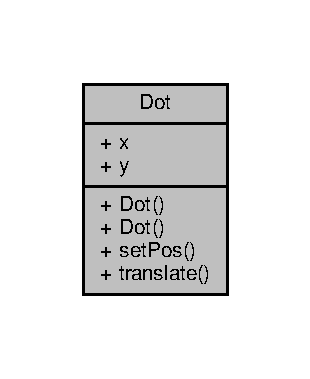
\includegraphics[width=149pt]{classDot__coll__graph}
\end{center}
\end{figure}
\subsubsection*{Fonctions membres publiques}
\begin{DoxyCompactItemize}
\item 
\hyperlink{classDot_ad7c02a05038699cfc7032f5a3c5340be}{Dot} (double \hyperlink{classDot_a2e1474ff16b86ce856a9f49d84a240d5}{x}, double \hyperlink{classDot_a17f640ad7b65953a11f602d0a8c6d162}{y})
\item 
\hyperlink{classDot_a04a7143246de78c09e00ff8ee3bb858a}{Dot} (double \hyperlink{classDot_a2e1474ff16b86ce856a9f49d84a240d5}{x}, double \hyperlink{classDot_a17f640ad7b65953a11f602d0a8c6d162}{y}, Boolean bol)
\item 
void \hyperlink{classDot_a59dbdc958aca411e9246125fb2b0e111}{set\+Pos} (int \hyperlink{classDot_a2e1474ff16b86ce856a9f49d84a240d5}{x}, int \hyperlink{classDot_a17f640ad7b65953a11f602d0a8c6d162}{y})
\item 
void \hyperlink{classDot_a06923e301e9bbf182833b1c4914f8d7d}{translate} ()
\end{DoxyCompactItemize}
\subsubsection*{Attributs publics}
\begin{DoxyCompactItemize}
\item 
int \hyperlink{classDot_a2e1474ff16b86ce856a9f49d84a240d5}{x}
\item 
int \hyperlink{classDot_a17f640ad7b65953a11f602d0a8c6d162}{y}
\end{DoxyCompactItemize}


\subsubsection{Documentation des constructeurs et destructeur}
\hypertarget{classDot_ad7c02a05038699cfc7032f5a3c5340be}{}\index{Dot@{Dot}!Dot@{Dot}}
\index{Dot@{Dot}!Dot@{Dot}}
\paragraph[{Dot}]{\setlength{\rightskip}{0pt plus 5cm}Dot.\+Dot (
\begin{DoxyParamCaption}
\item[{double}]{x, }
\item[{double}]{y}
\end{DoxyParamCaption}
)}\label{classDot_ad7c02a05038699cfc7032f5a3c5340be}
\hypertarget{classDot_a04a7143246de78c09e00ff8ee3bb858a}{}\index{Dot@{Dot}!Dot@{Dot}}
\index{Dot@{Dot}!Dot@{Dot}}
\paragraph[{Dot}]{\setlength{\rightskip}{0pt plus 5cm}Dot.\+Dot (
\begin{DoxyParamCaption}
\item[{double}]{x, }
\item[{double}]{y, }
\item[{Boolean}]{bol}
\end{DoxyParamCaption}
)}\label{classDot_a04a7143246de78c09e00ff8ee3bb858a}


\subsubsection{Documentation des fonctions membres}
\hypertarget{classDot_a59dbdc958aca411e9246125fb2b0e111}{}\index{Dot@{Dot}!set\+Pos@{set\+Pos}}
\index{set\+Pos@{set\+Pos}!Dot@{Dot}}
\paragraph[{set\+Pos}]{\setlength{\rightskip}{0pt plus 5cm}void Dot.\+set\+Pos (
\begin{DoxyParamCaption}
\item[{int}]{x, }
\item[{int}]{y}
\end{DoxyParamCaption}
)}\label{classDot_a59dbdc958aca411e9246125fb2b0e111}
\hypertarget{classDot_a06923e301e9bbf182833b1c4914f8d7d}{}\index{Dot@{Dot}!translate@{translate}}
\index{translate@{translate}!Dot@{Dot}}
\paragraph[{translate}]{\setlength{\rightskip}{0pt plus 5cm}void Dot.\+translate (
\begin{DoxyParamCaption}
{}
\end{DoxyParamCaption}
)}\label{classDot_a06923e301e9bbf182833b1c4914f8d7d}


Référencé par Dot().



\subsubsection{Documentation des données membres}
\hypertarget{classDot_a2e1474ff16b86ce856a9f49d84a240d5}{}\index{Dot@{Dot}!x@{x}}
\index{x@{x}!Dot@{Dot}}
\paragraph[{x}]{\setlength{\rightskip}{0pt plus 5cm}int Dot.\+x}\label{classDot_a2e1474ff16b86ce856a9f49d84a240d5}


Référencé par Read\+Zone.\+add\+Zone(), Screen.\+get\+Game\+Area(), Screen.\+look\+Horizontal(), Screen.\+look\+Vertical(), et set\+Pos().

\hypertarget{classDot_a17f640ad7b65953a11f602d0a8c6d162}{}\index{Dot@{Dot}!y@{y}}
\index{y@{y}!Dot@{Dot}}
\paragraph[{y}]{\setlength{\rightskip}{0pt plus 5cm}int Dot.\+y}\label{classDot_a17f640ad7b65953a11f602d0a8c6d162}


Référencé par Read\+Zone.\+add\+Zone(), Screen.\+get\+Game\+Area(), Screen.\+look\+Horizontal(), Screen.\+Screen(), et set\+Pos().



La documentation de cette classe a été générée à partir du fichier suivant \+:\begin{DoxyCompactItemize}
\item 
\hyperlink{oldCode_2Dot_8java}{old\+Code/\+Dot.\+java}\end{DoxyCompactItemize}

\hypertarget{classSuchi_1_1Dot}{}\subsection{Référence de la classe Suchi.\+Dot}
\label{classSuchi_1_1Dot}\index{Suchi.\+Dot@{Suchi.\+Dot}}


Graphe de collaboration de Suchi.\+Dot\+:\nopagebreak
\begin{figure}[H]
\begin{center}
\leavevmode
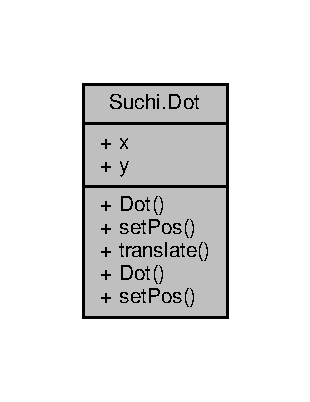
\includegraphics[width=149pt]{classSuchi_1_1Dot__coll__graph}
\end{center}
\end{figure}
\subsubsection*{Fonctions membres publiques}
\begin{DoxyCompactItemize}
\item 
\hyperlink{classSuchi_1_1Dot_a99f165eacf645707bc10cdbda82c2d09}{Dot} (double \hyperlink{classSuchi_1_1Dot_a4abd47b4ec16a1542ad3b75ddc1d760c}{x}, double \hyperlink{classSuchi_1_1Dot_aae7adce7564961a6fed16af1d2857b8b}{y})
\begin{DoxyCompactList}\small\item\em Constructeur. \end{DoxyCompactList}\item 
void \hyperlink{classSuchi_1_1Dot_acd41112feb44645d2801d7161f8dd0fc}{set\+Pos} (int \hyperlink{classSuchi_1_1Dot_a4abd47b4ec16a1542ad3b75ddc1d760c}{x}, int \hyperlink{classSuchi_1_1Dot_aae7adce7564961a6fed16af1d2857b8b}{y})
\begin{DoxyCompactList}\small\item\em Méthode pour changer la position du point. \end{DoxyCompactList}\item 
void \hyperlink{classSuchi_1_1Dot_ae154c81b917dba659ec91bf3ce3ac7be}{translate} ()
\begin{DoxyCompactList}\small\item\em Translate les coordonnée dans les coordonnées de la zone de jeu. \end{DoxyCompactList}\item 
\hyperlink{classSuchi_1_1Dot_aa62b79fe9f80948dce52747bcc009ac8}{Dot} (int \hyperlink{classSuchi_1_1Dot_a4abd47b4ec16a1542ad3b75ddc1d760c}{x}, int \hyperlink{classSuchi_1_1Dot_aae7adce7564961a6fed16af1d2857b8b}{y})
\item 
void \hyperlink{classSuchi_1_1Dot_acd41112feb44645d2801d7161f8dd0fc}{set\+Pos} (int \hyperlink{classSuchi_1_1Dot_a4abd47b4ec16a1542ad3b75ddc1d760c}{x}, int \hyperlink{classSuchi_1_1Dot_aae7adce7564961a6fed16af1d2857b8b}{y})
\end{DoxyCompactItemize}
\subsubsection*{Attributs publics}
\begin{DoxyCompactItemize}
\item 
int \hyperlink{classSuchi_1_1Dot_a4abd47b4ec16a1542ad3b75ddc1d760c}{x}
\item 
int \hyperlink{classSuchi_1_1Dot_aae7adce7564961a6fed16af1d2857b8b}{y}
\end{DoxyCompactItemize}


\subsubsection{Documentation des constructeurs et destructeur}
\hypertarget{classSuchi_1_1Dot_a99f165eacf645707bc10cdbda82c2d09}{}\index{Suchi\+::\+Dot@{Suchi\+::\+Dot}!Dot@{Dot}}
\index{Dot@{Dot}!Suchi\+::\+Dot@{Suchi\+::\+Dot}}
\paragraph[{Dot}]{\setlength{\rightskip}{0pt plus 5cm}Suchi.\+Dot.\+Dot (
\begin{DoxyParamCaption}
\item[{double}]{x, }
\item[{double}]{y}
\end{DoxyParamCaption}
)}\label{classSuchi_1_1Dot_a99f165eacf645707bc10cdbda82c2d09}


Constructeur. 


\begin{DoxyParams}{Paramètres}
{\em x} & Coordonnée x dans le repère de l\textquotesingle{}écran \\
\hline
{\em y} & Coordonnée y dans le repère de l\textquotesingle{}écran \\
\hline
\end{DoxyParams}
\hypertarget{classSuchi_1_1Dot_aa62b79fe9f80948dce52747bcc009ac8}{}\index{Suchi\+::\+Dot@{Suchi\+::\+Dot}!Dot@{Dot}}
\index{Dot@{Dot}!Suchi\+::\+Dot@{Suchi\+::\+Dot}}
\paragraph[{Dot}]{\setlength{\rightskip}{0pt plus 5cm}Suchi.\+Dot.\+Dot (
\begin{DoxyParamCaption}
\item[{int}]{x, }
\item[{int}]{y}
\end{DoxyParamCaption}
)}\label{classSuchi_1_1Dot_aa62b79fe9f80948dce52747bcc009ac8}


\subsubsection{Documentation des fonctions membres}
\hypertarget{classSuchi_1_1Dot_acd41112feb44645d2801d7161f8dd0fc}{}\index{Suchi\+::\+Dot@{Suchi\+::\+Dot}!set\+Pos@{set\+Pos}}
\index{set\+Pos@{set\+Pos}!Suchi\+::\+Dot@{Suchi\+::\+Dot}}
\paragraph[{set\+Pos}]{\setlength{\rightskip}{0pt plus 5cm}void Suchi.\+Dot.\+set\+Pos (
\begin{DoxyParamCaption}
\item[{int}]{x, }
\item[{int}]{y}
\end{DoxyParamCaption}
)}\label{classSuchi_1_1Dot_acd41112feb44645d2801d7161f8dd0fc}


Méthode pour changer la position du point. 


\begin{DoxyParams}{Paramètres}
{\em x} & \\
\hline
{\em y} & \\
\hline
\end{DoxyParams}
\hypertarget{classSuchi_1_1Dot_acd41112feb44645d2801d7161f8dd0fc}{}\index{Suchi\+::\+Dot@{Suchi\+::\+Dot}!set\+Pos@{set\+Pos}}
\index{set\+Pos@{set\+Pos}!Suchi\+::\+Dot@{Suchi\+::\+Dot}}
\paragraph[{set\+Pos}]{\setlength{\rightskip}{0pt plus 5cm}void Suchi.\+Dot.\+set\+Pos (
\begin{DoxyParamCaption}
\item[{int}]{x, }
\item[{int}]{y}
\end{DoxyParamCaption}
)}\label{classSuchi_1_1Dot_acd41112feb44645d2801d7161f8dd0fc}
\hypertarget{classSuchi_1_1Dot_ae154c81b917dba659ec91bf3ce3ac7be}{}\index{Suchi\+::\+Dot@{Suchi\+::\+Dot}!translate@{translate}}
\index{translate@{translate}!Suchi\+::\+Dot@{Suchi\+::\+Dot}}
\paragraph[{translate}]{\setlength{\rightskip}{0pt plus 5cm}void Suchi.\+Dot.\+translate (
\begin{DoxyParamCaption}
{}
\end{DoxyParamCaption}
)}\label{classSuchi_1_1Dot_ae154c81b917dba659ec91bf3ce3ac7be}


Translate les coordonnée dans les coordonnées de la zone de jeu. 



Référencé par Suchi.\+Dot.\+Dot().



\subsubsection{Documentation des données membres}
\hypertarget{classSuchi_1_1Dot_a4abd47b4ec16a1542ad3b75ddc1d760c}{}\index{Suchi\+::\+Dot@{Suchi\+::\+Dot}!x@{x}}
\index{x@{x}!Suchi\+::\+Dot@{Suchi\+::\+Dot}}
\paragraph[{x}]{\setlength{\rightskip}{0pt plus 5cm}int Dot.\+x}\label{classSuchi_1_1Dot_a4abd47b4ec16a1542ad3b75ddc1d760c}


Référencé par Pictures.\+Recon.\+add\+Zone(), Suchi.\+Dot.\+Dot(), Suchi.\+Ia.\+fill\+Commandes(), Suchi.\+Ia.\+fill\+Grey\+Table(), Suchi.\+Screen.\+get\+Game\+Area(), Suchi.\+Screen.\+look\+Horizontal(), Suchi.\+Screen.\+look\+Vertical(), Suchi.\+Dot.\+set\+Pos(), et Suchi.\+Game.\+set\+Zone\+Win().

\hypertarget{classSuchi_1_1Dot_aae7adce7564961a6fed16af1d2857b8b}{}\index{Suchi\+::\+Dot@{Suchi\+::\+Dot}!y@{y}}
\index{y@{y}!Suchi\+::\+Dot@{Suchi\+::\+Dot}}
\paragraph[{y}]{\setlength{\rightskip}{0pt plus 5cm}int Dot.\+y}\label{classSuchi_1_1Dot_aae7adce7564961a6fed16af1d2857b8b}


Référencé par Pictures.\+Recon.\+add\+Zone(), Suchi.\+Dot.\+Dot(), Suchi.\+Ia.\+fill\+Commandes(), Suchi.\+Ia.\+fill\+Grey\+Table(), Suchi.\+Screen.\+get\+Game\+Area(), Suchi.\+Screen.\+look\+Horizontal(), Suchi.\+Screen.\+Screen(), Suchi.\+Dot.\+set\+Pos(), et Suchi.\+Game.\+set\+Zone\+Win().



La documentation de cette classe a été générée à partir des fichiers suivants \+:\begin{DoxyCompactItemize}
\item 
\hyperlink{BotSofRetapage_2src_2Suchi_2Dot_8java}{Bot\+Sof\+Retapage/src/\+Suchi/\+Dot.\+java}\item 
\hyperlink{BotSuchis_2TestSuchis_2Suchi_2Screen_8java}{Bot\+Suchis/\+Test\+Suchis/\+Suchi/\+Screen.\+java}\end{DoxyCompactItemize}

\hypertarget{classmain_1_1Dot}{}\subsection{Référence de la classe main.\+Dot}
\label{classmain_1_1Dot}\index{main.\+Dot@{main.\+Dot}}


Graphe de collaboration de main.\+Dot\+:\nopagebreak
\begin{figure}[H]
\begin{center}
\leavevmode
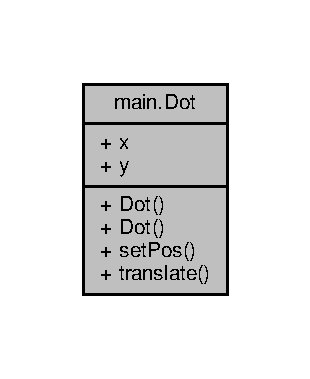
\includegraphics[width=149pt]{classmain_1_1Dot__coll__graph}
\end{center}
\end{figure}
\subsubsection*{Fonctions membres publiques}
\begin{DoxyCompactItemize}
\item 
\hyperlink{classmain_1_1Dot_a978f641727f59636f1bfc6aed8a0008a}{Dot} (double \hyperlink{classmain_1_1Dot_acfbfe11b1f5baa23f8b72bf26121d92e}{x}, double \hyperlink{classmain_1_1Dot_a34d8039b67ad611941a096e87a219fb1}{y})
\item 
\hyperlink{classmain_1_1Dot_abb292f333a2f38752bb881b3bb6e708f}{Dot} (double \hyperlink{classmain_1_1Dot_acfbfe11b1f5baa23f8b72bf26121d92e}{x}, double \hyperlink{classmain_1_1Dot_a34d8039b67ad611941a096e87a219fb1}{y}, Boolean bol)
\item 
void \hyperlink{classmain_1_1Dot_a457d705fcb68522e091d0f01a38a0bdb}{set\+Pos} (int \hyperlink{classmain_1_1Dot_acfbfe11b1f5baa23f8b72bf26121d92e}{x}, int \hyperlink{classmain_1_1Dot_a34d8039b67ad611941a096e87a219fb1}{y})
\item 
void \hyperlink{classmain_1_1Dot_ae490ac692da44edde94754ead7660aff}{translate} ()
\end{DoxyCompactItemize}
\subsubsection*{Attributs publics}
\begin{DoxyCompactItemize}
\item 
int \hyperlink{classmain_1_1Dot_acfbfe11b1f5baa23f8b72bf26121d92e}{x}
\item 
int \hyperlink{classmain_1_1Dot_a34d8039b67ad611941a096e87a219fb1}{y}
\end{DoxyCompactItemize}


\subsubsection{Documentation des constructeurs et destructeur}
\hypertarget{classmain_1_1Dot_a978f641727f59636f1bfc6aed8a0008a}{}\index{main\+::\+Dot@{main\+::\+Dot}!Dot@{Dot}}
\index{Dot@{Dot}!main\+::\+Dot@{main\+::\+Dot}}
\paragraph[{Dot}]{\setlength{\rightskip}{0pt plus 5cm}main.\+Dot.\+Dot (
\begin{DoxyParamCaption}
\item[{double}]{x, }
\item[{double}]{y}
\end{DoxyParamCaption}
)}\label{classmain_1_1Dot_a978f641727f59636f1bfc6aed8a0008a}
\hypertarget{classmain_1_1Dot_abb292f333a2f38752bb881b3bb6e708f}{}\index{main\+::\+Dot@{main\+::\+Dot}!Dot@{Dot}}
\index{Dot@{Dot}!main\+::\+Dot@{main\+::\+Dot}}
\paragraph[{Dot}]{\setlength{\rightskip}{0pt plus 5cm}main.\+Dot.\+Dot (
\begin{DoxyParamCaption}
\item[{double}]{x, }
\item[{double}]{y, }
\item[{Boolean}]{bol}
\end{DoxyParamCaption}
)}\label{classmain_1_1Dot_abb292f333a2f38752bb881b3bb6e708f}


\subsubsection{Documentation des fonctions membres}
\hypertarget{classmain_1_1Dot_a457d705fcb68522e091d0f01a38a0bdb}{}\index{main\+::\+Dot@{main\+::\+Dot}!set\+Pos@{set\+Pos}}
\index{set\+Pos@{set\+Pos}!main\+::\+Dot@{main\+::\+Dot}}
\paragraph[{set\+Pos}]{\setlength{\rightskip}{0pt plus 5cm}void main.\+Dot.\+set\+Pos (
\begin{DoxyParamCaption}
\item[{int}]{x, }
\item[{int}]{y}
\end{DoxyParamCaption}
)}\label{classmain_1_1Dot_a457d705fcb68522e091d0f01a38a0bdb}
\hypertarget{classmain_1_1Dot_ae490ac692da44edde94754ead7660aff}{}\index{main\+::\+Dot@{main\+::\+Dot}!translate@{translate}}
\index{translate@{translate}!main\+::\+Dot@{main\+::\+Dot}}
\paragraph[{translate}]{\setlength{\rightskip}{0pt plus 5cm}void main.\+Dot.\+translate (
\begin{DoxyParamCaption}
{}
\end{DoxyParamCaption}
)}\label{classmain_1_1Dot_ae490ac692da44edde94754ead7660aff}


Référencé par main.\+Dot.\+Dot().



\subsubsection{Documentation des données membres}
\hypertarget{classmain_1_1Dot_acfbfe11b1f5baa23f8b72bf26121d92e}{}\index{main\+::\+Dot@{main\+::\+Dot}!x@{x}}
\index{x@{x}!main\+::\+Dot@{main\+::\+Dot}}
\paragraph[{x}]{\setlength{\rightskip}{0pt plus 5cm}int main.\+Dot.\+x}\label{classmain_1_1Dot_acfbfe11b1f5baa23f8b72bf26121d92e}


Référencé par main.\+Read\+Zone.\+add\+Zone(), main.\+Screen.\+get\+Game\+Area(), main.\+Screen.\+look\+Horizontal(), main.\+Screen.\+look\+Vertical(), et main.\+Dot.\+set\+Pos().

\hypertarget{classmain_1_1Dot_a34d8039b67ad611941a096e87a219fb1}{}\index{main\+::\+Dot@{main\+::\+Dot}!y@{y}}
\index{y@{y}!main\+::\+Dot@{main\+::\+Dot}}
\paragraph[{y}]{\setlength{\rightskip}{0pt plus 5cm}int main.\+Dot.\+y}\label{classmain_1_1Dot_a34d8039b67ad611941a096e87a219fb1}


Référencé par main.\+Read\+Zone.\+add\+Zone(), main.\+Screen.\+get\+Game\+Area(), main.\+Screen.\+look\+Horizontal(), main.\+Screen.\+Screen(), et main.\+Dot.\+set\+Pos().



La documentation de cette classe a été générée à partir du fichier suivant \+:\begin{DoxyCompactItemize}
\item 
\hyperlink{main_2Dot_8java}{main/\+Dot.\+java}\end{DoxyCompactItemize}

\hypertarget{classTestSushi_1_1src_1_1Pictures_1_1FindPicture}{}\subsection{Référence de la classe Test\+Sushi.\+src.\+Pictures.\+Find\+Picture}
\label{classTestSushi_1_1src_1_1Pictures_1_1FindPicture}\index{Test\+Sushi.\+src.\+Pictures.\+Find\+Picture@{Test\+Sushi.\+src.\+Pictures.\+Find\+Picture}}


Graphe de collaboration de Test\+Sushi.\+src.\+Pictures.\+Find\+Picture\+:\nopagebreak
\begin{figure}[H]
\begin{center}
\leavevmode
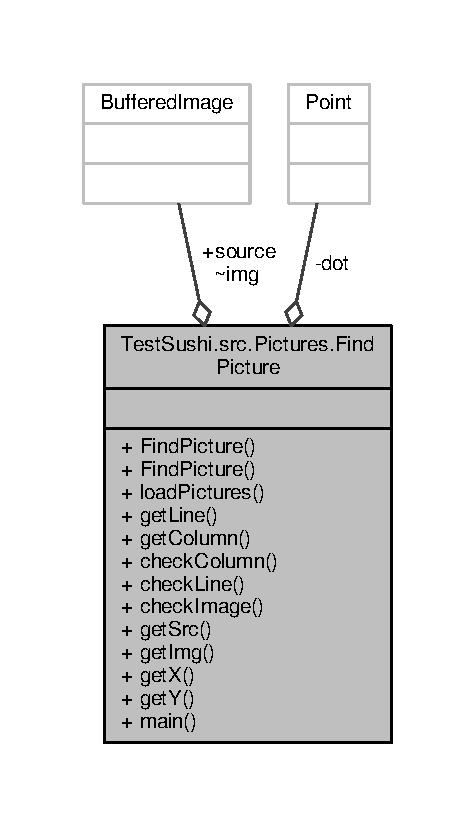
\includegraphics[width=228pt]{classTestSushi_1_1src_1_1Pictures_1_1FindPicture__coll__graph}
\end{center}
\end{figure}
\subsubsection*{Fonctions membres publiques}
\begin{DoxyCompactItemize}
\item 
\hyperlink{classTestSushi_1_1src_1_1Pictures_1_1FindPicture_abb6768894f5395ad3b39c53f11cb330f}{Find\+Picture} (Buffered\+Image src, String \hyperlink{classTestSushi_1_1src_1_1Pictures_1_1FindPicture_a2efdf9b4cf94ca02ddc955f9a205c090}{img})
\begin{DoxyCompactList}\small\item\em Constructeur. \end{DoxyCompactList}\item 
\hyperlink{classTestSushi_1_1src_1_1Pictures_1_1FindPicture_ab96ff4f810f4f3d3db16671b22e76e37}{Find\+Picture} (Buffered\+Image src, Buffered\+Image \hyperlink{classTestSushi_1_1src_1_1Pictures_1_1FindPicture_a2efdf9b4cf94ca02ddc955f9a205c090}{img})
\begin{DoxyCompactList}\small\item\em Constructeur. \end{DoxyCompactList}\item 
void \hyperlink{classTestSushi_1_1src_1_1Pictures_1_1FindPicture_a0a7343c194f8daa44221581414372266}{load\+Pictures} (String path\+Img)
\begin{DoxyCompactList}\small\item\em Méthode qui charge l\textquotesingle{}image à chercher dans img. \end{DoxyCompactList}\item 
Array\+List$<$ Integer $>$ \hyperlink{classTestSushi_1_1src_1_1Pictures_1_1FindPicture_a11da4bbb2dfb596d71001f68b95f9cbb}{get\+Line} (Buffered\+Image \hyperlink{classTestSushi_1_1src_1_1Pictures_1_1FindPicture_a2efdf9b4cf94ca02ddc955f9a205c090}{img}, int line)
\begin{DoxyCompactList}\small\item\em Méthode qui retourne une Array\+List qui contient la ligne sélectionné de l\textquotesingle{}image img. \end{DoxyCompactList}\item 
Array\+List$<$ Integer $>$ \hyperlink{classTestSushi_1_1src_1_1Pictures_1_1FindPicture_ab56e357271314618a65a0634005e3aea}{get\+Column} (Buffered\+Image \hyperlink{classTestSushi_1_1src_1_1Pictures_1_1FindPicture_a2efdf9b4cf94ca02ddc955f9a205c090}{img}, int column)
\begin{DoxyCompactList}\small\item\em Méthode qui retourne une Array\+List qui contient la colonne sélectionné de l\textquotesingle{}image img. \end{DoxyCompactList}\item 
boolean \hyperlink{classTestSushi_1_1src_1_1Pictures_1_1FindPicture_a56e9690469fb4e52c0576170379ff1a7}{check\+Column} (Buffered\+Image \hyperlink{classTestSushi_1_1src_1_1Pictures_1_1FindPicture_a8f97c27187060e065669476a0774be89}{source}, Buffered\+Image \hyperlink{classTestSushi_1_1src_1_1Pictures_1_1FindPicture_a2efdf9b4cf94ca02ddc955f9a205c090}{img})
\begin{DoxyCompactList}\small\item\em méthode qui vérifie si une certaine colonne de l\textquotesingle{}img se trouve dans source \end{DoxyCompactList}\item 
boolean \hyperlink{classTestSushi_1_1src_1_1Pictures_1_1FindPicture_adf02994bcf4a6a517aaf543714c746a3}{check\+Line} (Buffered\+Image \hyperlink{classTestSushi_1_1src_1_1Pictures_1_1FindPicture_a8f97c27187060e065669476a0774be89}{source}, Buffered\+Image \hyperlink{classTestSushi_1_1src_1_1Pictures_1_1FindPicture_a2efdf9b4cf94ca02ddc955f9a205c090}{img})
\begin{DoxyCompactList}\small\item\em méthode qui vérifie si une certaine ligne de l\textquotesingle{}img se trouve dans source \end{DoxyCompactList}\item 
boolean \hyperlink{classTestSushi_1_1src_1_1Pictures_1_1FindPicture_ab474926b25aa877731dd0476b99dd42a}{check\+Image} ()
\begin{DoxyCompactList}\small\item\em Vérifie si l\textquotesingle{}img existe dans source. \end{DoxyCompactList}\item 
Buffered\+Image \hyperlink{classTestSushi_1_1src_1_1Pictures_1_1FindPicture_adc71f6e660e967e95f429cee5f27fa55}{get\+Src} ()
\begin{DoxyCompactList}\small\item\em Renvoie l\textquotesingle{}image source de l\textquotesingle{}objet. \end{DoxyCompactList}\item 
Buffered\+Image \hyperlink{classTestSushi_1_1src_1_1Pictures_1_1FindPicture_a8d91848dc7a2eaea672ae3ee3a0caa56}{get\+Img} ()
\begin{DoxyCompactList}\small\item\em Renvoie l\textquotesingle{}image img de l\textquotesingle{}objet. \end{DoxyCompactList}\item 
int \hyperlink{classTestSushi_1_1src_1_1Pictures_1_1FindPicture_aeaee91c49573639fb996740f9536b383}{get\+X} ()
\begin{DoxyCompactList}\small\item\em Renvoie la coordonnée y. \end{DoxyCompactList}\item 
int \hyperlink{classTestSushi_1_1src_1_1Pictures_1_1FindPicture_a9b3afe70eaccc3ba4151d8b3926fb27c}{get\+Y} ()
\begin{DoxyCompactList}\small\item\em Renovie la coordonnée y. \end{DoxyCompactList}\end{DoxyCompactItemize}
\subsubsection*{Fonctions membres publiques statiques}
\begin{DoxyCompactItemize}
\item 
static void \hyperlink{classTestSushi_1_1src_1_1Pictures_1_1FindPicture_a7ebd0b729a5146cfdc91c4b367c817af}{main} (String\mbox{[}$\,$\mbox{]} s)
\end{DoxyCompactItemize}
\subsubsection*{Attributs publics}
\begin{DoxyCompactItemize}
\item 
Buffered\+Image \hyperlink{classTestSushi_1_1src_1_1Pictures_1_1FindPicture_a8f97c27187060e065669476a0774be89}{source}
\end{DoxyCompactItemize}
\subsubsection*{Attributs de paquetage}
\begin{DoxyCompactItemize}
\item 
Buffered\+Image \hyperlink{classTestSushi_1_1src_1_1Pictures_1_1FindPicture_a2efdf9b4cf94ca02ddc955f9a205c090}{img}
\end{DoxyCompactItemize}
\subsubsection*{Attributs privés}
\begin{DoxyCompactItemize}
\item 
Point \hyperlink{classTestSushi_1_1src_1_1Pictures_1_1FindPicture_a11d5ad9f9638c38bdedea6033fef44bf}{dot}
\end{DoxyCompactItemize}


\subsubsection{Documentation des constructeurs et destructeur}
\hypertarget{classTestSushi_1_1src_1_1Pictures_1_1FindPicture_abb6768894f5395ad3b39c53f11cb330f}{}\index{Test\+Sushi\+::src\+::\+Pictures\+::\+Find\+Picture@{Test\+Sushi\+::src\+::\+Pictures\+::\+Find\+Picture}!Find\+Picture@{Find\+Picture}}
\index{Find\+Picture@{Find\+Picture}!Test\+Sushi\+::src\+::\+Pictures\+::\+Find\+Picture@{Test\+Sushi\+::src\+::\+Pictures\+::\+Find\+Picture}}
\paragraph[{Find\+Picture}]{\setlength{\rightskip}{0pt plus 5cm}Test\+Sushi.\+src.\+Pictures.\+Find\+Picture.\+Find\+Picture (
\begin{DoxyParamCaption}
\item[{Buffered\+Image}]{src, }
\item[{String}]{img}
\end{DoxyParamCaption}
)}\label{classTestSushi_1_1src_1_1Pictures_1_1FindPicture_abb6768894f5395ad3b39c53f11cb330f}


Constructeur. 


\begin{DoxyParams}{Paramètres}
{\em src} & Buffered\+Image de l\textquotesingle{}image sur laquelle chercher \\
\hline
{\em img} & path vers l\textquotesingle{}image à chercher dans l\textquotesingle{}image \\
\hline
\end{DoxyParams}


Référencé par Test\+Sushi.\+src.\+Pictures.\+Find\+Picture.\+main().

\hypertarget{classTestSushi_1_1src_1_1Pictures_1_1FindPicture_ab96ff4f810f4f3d3db16671b22e76e37}{}\index{Test\+Sushi\+::src\+::\+Pictures\+::\+Find\+Picture@{Test\+Sushi\+::src\+::\+Pictures\+::\+Find\+Picture}!Find\+Picture@{Find\+Picture}}
\index{Find\+Picture@{Find\+Picture}!Test\+Sushi\+::src\+::\+Pictures\+::\+Find\+Picture@{Test\+Sushi\+::src\+::\+Pictures\+::\+Find\+Picture}}
\paragraph[{Find\+Picture}]{\setlength{\rightskip}{0pt plus 5cm}Test\+Sushi.\+src.\+Pictures.\+Find\+Picture.\+Find\+Picture (
\begin{DoxyParamCaption}
\item[{Buffered\+Image}]{src, }
\item[{Buffered\+Image}]{img}
\end{DoxyParamCaption}
)}\label{classTestSushi_1_1src_1_1Pictures_1_1FindPicture_ab96ff4f810f4f3d3db16671b22e76e37}


Constructeur. 


\begin{DoxyParams}{Paramètres}
{\em src} & Buffered\+Image de l\textquotesingle{}image sur laquelle chercher \\
\hline
{\em img} & Buffered\+Image de l\textquotesingle{}image à chercher \\
\hline
\end{DoxyParams}


\subsubsection{Documentation des fonctions membres}
\hypertarget{classTestSushi_1_1src_1_1Pictures_1_1FindPicture_a56e9690469fb4e52c0576170379ff1a7}{}\index{Test\+Sushi\+::src\+::\+Pictures\+::\+Find\+Picture@{Test\+Sushi\+::src\+::\+Pictures\+::\+Find\+Picture}!check\+Column@{check\+Column}}
\index{check\+Column@{check\+Column}!Test\+Sushi\+::src\+::\+Pictures\+::\+Find\+Picture@{Test\+Sushi\+::src\+::\+Pictures\+::\+Find\+Picture}}
\paragraph[{check\+Column}]{\setlength{\rightskip}{0pt plus 5cm}boolean Test\+Sushi.\+src.\+Pictures.\+Find\+Picture.\+check\+Column (
\begin{DoxyParamCaption}
\item[{Buffered\+Image}]{source, }
\item[{Buffered\+Image}]{img}
\end{DoxyParamCaption}
)}\label{classTestSushi_1_1src_1_1Pictures_1_1FindPicture_a56e9690469fb4e52c0576170379ff1a7}


méthode qui vérifie si une certaine colonne de l\textquotesingle{}img se trouve dans source 


\begin{DoxyParams}{Paramètres}
{\em source} & L\textquotesingle{}image source dans laquelle chercher \\
\hline
{\em img} & L\textquotesingle{}image dont une colonne va être chercher \\
\hline
\end{DoxyParams}
\begin{DoxyReturn}{Renvoie}
true si la colonne existe dans source, false sinon 
\end{DoxyReturn}


Référencé par Test\+Sushi.\+src.\+Pictures.\+Find\+Picture.\+check\+Image(), et Test\+Sushi.\+src.\+Pictures.\+Find\+Picture.\+main().

\hypertarget{classTestSushi_1_1src_1_1Pictures_1_1FindPicture_ab474926b25aa877731dd0476b99dd42a}{}\index{Test\+Sushi\+::src\+::\+Pictures\+::\+Find\+Picture@{Test\+Sushi\+::src\+::\+Pictures\+::\+Find\+Picture}!check\+Image@{check\+Image}}
\index{check\+Image@{check\+Image}!Test\+Sushi\+::src\+::\+Pictures\+::\+Find\+Picture@{Test\+Sushi\+::src\+::\+Pictures\+::\+Find\+Picture}}
\paragraph[{check\+Image}]{\setlength{\rightskip}{0pt plus 5cm}boolean Test\+Sushi.\+src.\+Pictures.\+Find\+Picture.\+check\+Image (
\begin{DoxyParamCaption}
{}
\end{DoxyParamCaption}
)}\label{classTestSushi_1_1src_1_1Pictures_1_1FindPicture_ab474926b25aa877731dd0476b99dd42a}


Vérifie si l\textquotesingle{}img existe dans source. 

\begin{DoxyReturn}{Renvoie}
true si l\textquotesingle{}image chercher se trouve dans l\textquotesingle{}image, false sinon 
\end{DoxyReturn}


Référencé par Test\+Sushi.\+src.\+Suchi.\+Recette.\+buy\+Noori(), Test\+Sushi.\+src.\+Suchi.\+Recette.\+buy\+Rice(), Test\+Sushi.\+src.\+Suchi.\+Recette.\+buy\+Roe(), Test\+Sushi.\+src.\+Suchi.\+Recette.\+buy\+Salmon(), Test\+Sushi.\+src.\+Suchi.\+Recette.\+buy\+Shrimp(), Test\+Sushi.\+src.\+Suchi.\+Client.\+check(), Test\+Sushi.\+src.\+Suchi.\+Game.\+you\+Win\+Level1(), et Test\+Sushi.\+src.\+Suchi.\+Game.\+you\+Win\+Level2().

\hypertarget{classTestSushi_1_1src_1_1Pictures_1_1FindPicture_adf02994bcf4a6a517aaf543714c746a3}{}\index{Test\+Sushi\+::src\+::\+Pictures\+::\+Find\+Picture@{Test\+Sushi\+::src\+::\+Pictures\+::\+Find\+Picture}!check\+Line@{check\+Line}}
\index{check\+Line@{check\+Line}!Test\+Sushi\+::src\+::\+Pictures\+::\+Find\+Picture@{Test\+Sushi\+::src\+::\+Pictures\+::\+Find\+Picture}}
\paragraph[{check\+Line}]{\setlength{\rightskip}{0pt plus 5cm}boolean Test\+Sushi.\+src.\+Pictures.\+Find\+Picture.\+check\+Line (
\begin{DoxyParamCaption}
\item[{Buffered\+Image}]{source, }
\item[{Buffered\+Image}]{img}
\end{DoxyParamCaption}
)}\label{classTestSushi_1_1src_1_1Pictures_1_1FindPicture_adf02994bcf4a6a517aaf543714c746a3}


méthode qui vérifie si une certaine ligne de l\textquotesingle{}img se trouve dans source 


\begin{DoxyParams}{Paramètres}
{\em source} & L\textquotesingle{}image source dans laquelle chercher \\
\hline
{\em img} & L\textquotesingle{}image dont une colonne va être chercher \\
\hline
\end{DoxyParams}
\begin{DoxyReturn}{Renvoie}
true si la ligne existe dans source, false sinon 
\end{DoxyReturn}


Référencé par Test\+Sushi.\+src.\+Pictures.\+Find\+Picture.\+check\+Image(), et Test\+Sushi.\+src.\+Pictures.\+Find\+Picture.\+main().

\hypertarget{classTestSushi_1_1src_1_1Pictures_1_1FindPicture_ab56e357271314618a65a0634005e3aea}{}\index{Test\+Sushi\+::src\+::\+Pictures\+::\+Find\+Picture@{Test\+Sushi\+::src\+::\+Pictures\+::\+Find\+Picture}!get\+Column@{get\+Column}}
\index{get\+Column@{get\+Column}!Test\+Sushi\+::src\+::\+Pictures\+::\+Find\+Picture@{Test\+Sushi\+::src\+::\+Pictures\+::\+Find\+Picture}}
\paragraph[{get\+Column}]{\setlength{\rightskip}{0pt plus 5cm}Array\+List$<$Integer$>$ Test\+Sushi.\+src.\+Pictures.\+Find\+Picture.\+get\+Column (
\begin{DoxyParamCaption}
\item[{Buffered\+Image}]{img, }
\item[{int}]{column}
\end{DoxyParamCaption}
)}\label{classTestSushi_1_1src_1_1Pictures_1_1FindPicture_ab56e357271314618a65a0634005e3aea}


Méthode qui retourne une Array\+List qui contient la colonne sélectionné de l\textquotesingle{}image img. 


\begin{DoxyParams}{Paramètres}
{\em img} & L\textquotesingle{}image sur laquelle travailler \\
\hline
{\em column} & Le numéro de la colonne à prendre \\
\hline
\end{DoxyParams}
\begin{DoxyReturn}{Renvoie}
Array\+List qui contient les pixels de la colonne sélectionné 
\end{DoxyReturn}


Référencé par Test\+Sushi.\+src.\+Pictures.\+Find\+Picture.\+check\+Column().

\hypertarget{classTestSushi_1_1src_1_1Pictures_1_1FindPicture_a8d91848dc7a2eaea672ae3ee3a0caa56}{}\index{Test\+Sushi\+::src\+::\+Pictures\+::\+Find\+Picture@{Test\+Sushi\+::src\+::\+Pictures\+::\+Find\+Picture}!get\+Img@{get\+Img}}
\index{get\+Img@{get\+Img}!Test\+Sushi\+::src\+::\+Pictures\+::\+Find\+Picture@{Test\+Sushi\+::src\+::\+Pictures\+::\+Find\+Picture}}
\paragraph[{get\+Img}]{\setlength{\rightskip}{0pt plus 5cm}Buffered\+Image Test\+Sushi.\+src.\+Pictures.\+Find\+Picture.\+get\+Img (
\begin{DoxyParamCaption}
{}
\end{DoxyParamCaption}
)}\label{classTestSushi_1_1src_1_1Pictures_1_1FindPicture_a8d91848dc7a2eaea672ae3ee3a0caa56}


Renvoie l\textquotesingle{}image img de l\textquotesingle{}objet. 

\begin{DoxyReturn}{Renvoie}

\end{DoxyReturn}


Référencé par Test\+Sushi.\+src.\+Pictures.\+Find\+Picture.\+check\+Image().

\hypertarget{classTestSushi_1_1src_1_1Pictures_1_1FindPicture_a11da4bbb2dfb596d71001f68b95f9cbb}{}\index{Test\+Sushi\+::src\+::\+Pictures\+::\+Find\+Picture@{Test\+Sushi\+::src\+::\+Pictures\+::\+Find\+Picture}!get\+Line@{get\+Line}}
\index{get\+Line@{get\+Line}!Test\+Sushi\+::src\+::\+Pictures\+::\+Find\+Picture@{Test\+Sushi\+::src\+::\+Pictures\+::\+Find\+Picture}}
\paragraph[{get\+Line}]{\setlength{\rightskip}{0pt plus 5cm}Array\+List$<$Integer$>$ Test\+Sushi.\+src.\+Pictures.\+Find\+Picture.\+get\+Line (
\begin{DoxyParamCaption}
\item[{Buffered\+Image}]{img, }
\item[{int}]{line}
\end{DoxyParamCaption}
)}\label{classTestSushi_1_1src_1_1Pictures_1_1FindPicture_a11da4bbb2dfb596d71001f68b95f9cbb}


Méthode qui retourne une Array\+List qui contient la ligne sélectionné de l\textquotesingle{}image img. 


\begin{DoxyParams}{Paramètres}
{\em img} & L\textquotesingle{}image sur laquelle travailler \\
\hline
{\em line} & Le numéro de la ligne à prendre \\
\hline
\end{DoxyParams}
\begin{DoxyReturn}{Renvoie}
Array\+List qui contient les pixels de la ligne sélectionné 
\end{DoxyReturn}


Référencé par Test\+Sushi.\+src.\+Pictures.\+Find\+Picture.\+check\+Line().

\hypertarget{classTestSushi_1_1src_1_1Pictures_1_1FindPicture_adc71f6e660e967e95f429cee5f27fa55}{}\index{Test\+Sushi\+::src\+::\+Pictures\+::\+Find\+Picture@{Test\+Sushi\+::src\+::\+Pictures\+::\+Find\+Picture}!get\+Src@{get\+Src}}
\index{get\+Src@{get\+Src}!Test\+Sushi\+::src\+::\+Pictures\+::\+Find\+Picture@{Test\+Sushi\+::src\+::\+Pictures\+::\+Find\+Picture}}
\paragraph[{get\+Src}]{\setlength{\rightskip}{0pt plus 5cm}Buffered\+Image Test\+Sushi.\+src.\+Pictures.\+Find\+Picture.\+get\+Src (
\begin{DoxyParamCaption}
{}
\end{DoxyParamCaption}
)}\label{classTestSushi_1_1src_1_1Pictures_1_1FindPicture_adc71f6e660e967e95f429cee5f27fa55}


Renvoie l\textquotesingle{}image source de l\textquotesingle{}objet. 

\begin{DoxyReturn}{Renvoie}

\end{DoxyReturn}


Référencé par Test\+Sushi.\+src.\+Pictures.\+Find\+Picture.\+check\+Image().

\hypertarget{classTestSushi_1_1src_1_1Pictures_1_1FindPicture_aeaee91c49573639fb996740f9536b383}{}\index{Test\+Sushi\+::src\+::\+Pictures\+::\+Find\+Picture@{Test\+Sushi\+::src\+::\+Pictures\+::\+Find\+Picture}!get\+X@{get\+X}}
\index{get\+X@{get\+X}!Test\+Sushi\+::src\+::\+Pictures\+::\+Find\+Picture@{Test\+Sushi\+::src\+::\+Pictures\+::\+Find\+Picture}}
\paragraph[{get\+X}]{\setlength{\rightskip}{0pt plus 5cm}int Test\+Sushi.\+src.\+Pictures.\+Find\+Picture.\+get\+X (
\begin{DoxyParamCaption}
{}
\end{DoxyParamCaption}
)}\label{classTestSushi_1_1src_1_1Pictures_1_1FindPicture_aeaee91c49573639fb996740f9536b383}


Renvoie la coordonnée y. 

\begin{DoxyReturn}{Renvoie}

\end{DoxyReturn}


Référencé par Test\+Sushi.\+src.\+Pictures.\+Find\+Picture.\+check\+Image(), et Test\+Sushi.\+src.\+Pictures.\+Find\+Picture.\+main().

\hypertarget{classTestSushi_1_1src_1_1Pictures_1_1FindPicture_a9b3afe70eaccc3ba4151d8b3926fb27c}{}\index{Test\+Sushi\+::src\+::\+Pictures\+::\+Find\+Picture@{Test\+Sushi\+::src\+::\+Pictures\+::\+Find\+Picture}!get\+Y@{get\+Y}}
\index{get\+Y@{get\+Y}!Test\+Sushi\+::src\+::\+Pictures\+::\+Find\+Picture@{Test\+Sushi\+::src\+::\+Pictures\+::\+Find\+Picture}}
\paragraph[{get\+Y}]{\setlength{\rightskip}{0pt plus 5cm}int Test\+Sushi.\+src.\+Pictures.\+Find\+Picture.\+get\+Y (
\begin{DoxyParamCaption}
{}
\end{DoxyParamCaption}
)}\label{classTestSushi_1_1src_1_1Pictures_1_1FindPicture_a9b3afe70eaccc3ba4151d8b3926fb27c}


Renovie la coordonnée y. 

\begin{DoxyReturn}{Renvoie}

\end{DoxyReturn}


Référencé par Test\+Sushi.\+src.\+Pictures.\+Find\+Picture.\+check\+Image(), et Test\+Sushi.\+src.\+Pictures.\+Find\+Picture.\+main().

\hypertarget{classTestSushi_1_1src_1_1Pictures_1_1FindPicture_a0a7343c194f8daa44221581414372266}{}\index{Test\+Sushi\+::src\+::\+Pictures\+::\+Find\+Picture@{Test\+Sushi\+::src\+::\+Pictures\+::\+Find\+Picture}!load\+Pictures@{load\+Pictures}}
\index{load\+Pictures@{load\+Pictures}!Test\+Sushi\+::src\+::\+Pictures\+::\+Find\+Picture@{Test\+Sushi\+::src\+::\+Pictures\+::\+Find\+Picture}}
\paragraph[{load\+Pictures}]{\setlength{\rightskip}{0pt plus 5cm}void Test\+Sushi.\+src.\+Pictures.\+Find\+Picture.\+load\+Pictures (
\begin{DoxyParamCaption}
\item[{String}]{path\+Img}
\end{DoxyParamCaption}
)}\label{classTestSushi_1_1src_1_1Pictures_1_1FindPicture_a0a7343c194f8daa44221581414372266}


Méthode qui charge l\textquotesingle{}image à chercher dans img. 


\begin{DoxyParams}{Paramètres}
{\em path\+Img} & Chemin vers l\textquotesingle{}image à chargé \\
\hline
\end{DoxyParams}


Référencé par Test\+Sushi.\+src.\+Suchi.\+Client.\+check(), et Test\+Sushi.\+src.\+Pictures.\+Find\+Picture.\+Find\+Picture().

\hypertarget{classTestSushi_1_1src_1_1Pictures_1_1FindPicture_a7ebd0b729a5146cfdc91c4b367c817af}{}\index{Test\+Sushi\+::src\+::\+Pictures\+::\+Find\+Picture@{Test\+Sushi\+::src\+::\+Pictures\+::\+Find\+Picture}!main@{main}}
\index{main@{main}!Test\+Sushi\+::src\+::\+Pictures\+::\+Find\+Picture@{Test\+Sushi\+::src\+::\+Pictures\+::\+Find\+Picture}}
\paragraph[{main}]{\setlength{\rightskip}{0pt plus 5cm}static void Test\+Sushi.\+src.\+Pictures.\+Find\+Picture.\+main (
\begin{DoxyParamCaption}
\item[{String\mbox{[}$\,$\mbox{]}}]{s}
\end{DoxyParamCaption}
)\hspace{0.3cm}{\ttfamily [static]}}\label{classTestSushi_1_1src_1_1Pictures_1_1FindPicture_a7ebd0b729a5146cfdc91c4b367c817af}


\subsubsection{Documentation des données membres}
\hypertarget{classTestSushi_1_1src_1_1Pictures_1_1FindPicture_a11d5ad9f9638c38bdedea6033fef44bf}{}\index{Test\+Sushi\+::src\+::\+Pictures\+::\+Find\+Picture@{Test\+Sushi\+::src\+::\+Pictures\+::\+Find\+Picture}!dot@{dot}}
\index{dot@{dot}!Test\+Sushi\+::src\+::\+Pictures\+::\+Find\+Picture@{Test\+Sushi\+::src\+::\+Pictures\+::\+Find\+Picture}}
\paragraph[{dot}]{\setlength{\rightskip}{0pt plus 5cm}Point Test\+Sushi.\+src.\+Pictures.\+Find\+Picture.\+dot\hspace{0.3cm}{\ttfamily [private]}}\label{classTestSushi_1_1src_1_1Pictures_1_1FindPicture_a11d5ad9f9638c38bdedea6033fef44bf}
\hypertarget{classTestSushi_1_1src_1_1Pictures_1_1FindPicture_a2efdf9b4cf94ca02ddc955f9a205c090}{}\index{Test\+Sushi\+::src\+::\+Pictures\+::\+Find\+Picture@{Test\+Sushi\+::src\+::\+Pictures\+::\+Find\+Picture}!img@{img}}
\index{img@{img}!Test\+Sushi\+::src\+::\+Pictures\+::\+Find\+Picture@{Test\+Sushi\+::src\+::\+Pictures\+::\+Find\+Picture}}
\paragraph[{img}]{\setlength{\rightskip}{0pt plus 5cm}Buffered\+Image Test\+Sushi.\+src.\+Pictures.\+Find\+Picture.\+img\hspace{0.3cm}{\ttfamily [package]}}\label{classTestSushi_1_1src_1_1Pictures_1_1FindPicture_a2efdf9b4cf94ca02ddc955f9a205c090}


Référencé par Test\+Sushi.\+src.\+Pictures.\+Find\+Picture.\+Find\+Picture(), Test\+Sushi.\+src.\+Pictures.\+Find\+Picture.\+get\+Img(), et Test\+Sushi.\+src.\+Pictures.\+Find\+Picture.\+main().

\hypertarget{classTestSushi_1_1src_1_1Pictures_1_1FindPicture_a8f97c27187060e065669476a0774be89}{}\index{Test\+Sushi\+::src\+::\+Pictures\+::\+Find\+Picture@{Test\+Sushi\+::src\+::\+Pictures\+::\+Find\+Picture}!source@{source}}
\index{source@{source}!Test\+Sushi\+::src\+::\+Pictures\+::\+Find\+Picture@{Test\+Sushi\+::src\+::\+Pictures\+::\+Find\+Picture}}
\paragraph[{source}]{\setlength{\rightskip}{0pt plus 5cm}Buffered\+Image Test\+Sushi.\+src.\+Pictures.\+Find\+Picture.\+source}\label{classTestSushi_1_1src_1_1Pictures_1_1FindPicture_a8f97c27187060e065669476a0774be89}


Référencé par Test\+Sushi.\+src.\+Pictures.\+Find\+Picture.\+get\+Src(), et Test\+Sushi.\+src.\+Pictures.\+Find\+Picture.\+main().



La documentation de cette classe a été générée à partir du fichier suivant \+:\begin{DoxyCompactItemize}
\item 
\hyperlink{projet_2TestSushi_2src_2Pictures_2FindPicture_8java}{projet/\+Test\+Sushi/src/\+Pictures/\+Find\+Picture.\+java}\end{DoxyCompactItemize}

\hypertarget{classPictures_1_1FindPicture}{}\subsection{Référence de la classe Pictures.\+Find\+Picture}
\label{classPictures_1_1FindPicture}\index{Pictures.\+Find\+Picture@{Pictures.\+Find\+Picture}}


Graphe de collaboration de Pictures.\+Find\+Picture\+:\nopagebreak
\begin{figure}[H]
\begin{center}
\leavevmode
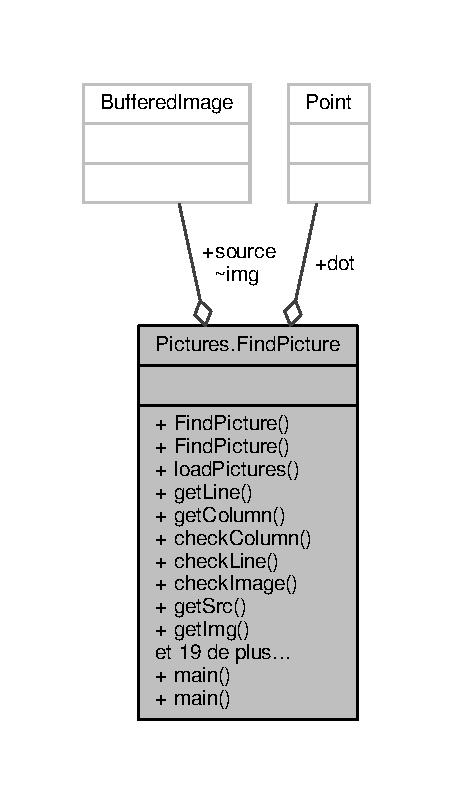
\includegraphics[width=218pt]{classPictures_1_1FindPicture__coll__graph}
\end{center}
\end{figure}
\subsubsection*{Fonctions membres publiques}
\begin{DoxyCompactItemize}
\item 
\hyperlink{classPictures_1_1FindPicture_a913868e0545034f6dca13d4b5b601d39}{Find\+Picture} (Buffered\+Image src, String \hyperlink{classPictures_1_1FindPicture_aae63a27df999ed48e5af4c680c3d75ad}{img})
\begin{DoxyCompactList}\small\item\em Constructeur. \end{DoxyCompactList}\item 
\hyperlink{classPictures_1_1FindPicture_a86b1b0b63cac91983b0ce92a17eefaba}{Find\+Picture} (Buffered\+Image src, Buffered\+Image \hyperlink{classPictures_1_1FindPicture_aae63a27df999ed48e5af4c680c3d75ad}{img})
\begin{DoxyCompactList}\small\item\em Constructeur. \end{DoxyCompactList}\item 
void \hyperlink{classPictures_1_1FindPicture_af0b1bc80dfd98aea65b056235702c3b4}{load\+Pictures} (String path\+Img)
\begin{DoxyCompactList}\small\item\em Méthode qui permet de charge un sprite dans le Buffered\+Image approprié \end{DoxyCompactList}\item 
Array\+List$<$ Integer $>$ \hyperlink{classPictures_1_1FindPicture_af6dbfb9eebba6ecaefb4c8c196cc3ccb}{get\+Line} (Buffered\+Image \hyperlink{classPictures_1_1FindPicture_aae63a27df999ed48e5af4c680c3d75ad}{img}, int line)
\begin{DoxyCompactList}\small\item\em Méthode qui renvoie l\textquotesingle{}Array\+List qui contient la ligne \char`\"{}line\char`\"{} dans l\textquotesingle{}image \char`\"{}img\char`\"{}. \end{DoxyCompactList}\item 
Array\+List$<$ Integer $>$ \hyperlink{classPictures_1_1FindPicture_a604c9cb11133f9910028abda35352255}{get\+Column} (Buffered\+Image \hyperlink{classPictures_1_1FindPicture_aae63a27df999ed48e5af4c680c3d75ad}{img}, int column)
\begin{DoxyCompactList}\small\item\em Méthode qui renvoie l\textquotesingle{}Array\+List qui contient la colonne \char`\"{}column\char`\"{} dans l\textquotesingle{}image \char`\"{}img\char`\"{}. \end{DoxyCompactList}\item 
boolean \hyperlink{classPictures_1_1FindPicture_ac0efebd74276c04a99d52535a4494337}{check\+Column} (Buffered\+Image \hyperlink{classPictures_1_1FindPicture_a97e21e6354d181ae52c8b33ff3968128}{source}, Buffered\+Image \hyperlink{classPictures_1_1FindPicture_aae63a27df999ed48e5af4c680c3d75ad}{img})
\begin{DoxyCompactList}\small\item\em On vérifie si la colonne au milieu du sprite se trouve dans l\textquotesingle{}image. \end{DoxyCompactList}\item 
boolean \hyperlink{classPictures_1_1FindPicture_af05439ba5284ef81cdc0bc2ee4f76eac}{check\+Line} (Buffered\+Image \hyperlink{classPictures_1_1FindPicture_a97e21e6354d181ae52c8b33ff3968128}{source}, Buffered\+Image \hyperlink{classPictures_1_1FindPicture_aae63a27df999ed48e5af4c680c3d75ad}{img})
\begin{DoxyCompactList}\small\item\em On vérifie si la ligne au milieu du sprite se trouve dans l\textquotesingle{}image. \end{DoxyCompactList}\item 
boolean \hyperlink{classPictures_1_1FindPicture_aad1e5b8e980b71a682633a78331a4579}{check\+Image} ()
\begin{DoxyCompactList}\small\item\em Méthode qui vérifie si le sprite chargé se trouve dans l\textquotesingle{}image également chargé \end{DoxyCompactList}\item 
Buffered\+Image \hyperlink{classPictures_1_1FindPicture_a7ffaa7ffcd58482dcc7050200a964608}{get\+Src} ()
\begin{DoxyCompactList}\small\item\em Accesseur vers l\textquotesingle{}image source. \end{DoxyCompactList}\item 
Buffered\+Image \hyperlink{classPictures_1_1FindPicture_a8e72367088f376429ac47d29c8a3112f}{get\+Img} ()
\begin{DoxyCompactList}\small\item\em Accesseur vers l\textquotesingle{}image du sprite. \end{DoxyCompactList}\item 
int \hyperlink{classPictures_1_1FindPicture_a80c3dda20e857d68aceacba5f5e0022e}{get\+X} ()
\begin{DoxyCompactList}\small\item\em Accesseur vers la coordonnée x. \end{DoxyCompactList}\item 
int \hyperlink{classPictures_1_1FindPicture_a8f340bb45086f386e0a3b8f91bc34d7d}{get\+Y} ()
\begin{DoxyCompactList}\small\item\em Accesseur vers la coordonnée y. \end{DoxyCompactList}\item 
\hyperlink{classPictures_1_1FindPicture_a913868e0545034f6dca13d4b5b601d39}{Find\+Picture} (Buffered\+Image src, String \hyperlink{classPictures_1_1FindPicture_aae63a27df999ed48e5af4c680c3d75ad}{img})
\item 
\hyperlink{classPictures_1_1FindPicture_a86b1b0b63cac91983b0ce92a17eefaba}{Find\+Picture} (Buffered\+Image src, Buffered\+Image \hyperlink{classPictures_1_1FindPicture_aae63a27df999ed48e5af4c680c3d75ad}{img})
\item 
void \hyperlink{classPictures_1_1FindPicture_af0b1bc80dfd98aea65b056235702c3b4}{load\+Pictures} (String path\+Img)
\item 
Array\+List$<$ Integer $>$ \hyperlink{classPictures_1_1FindPicture_af6dbfb9eebba6ecaefb4c8c196cc3ccb}{get\+Line} (Buffered\+Image \hyperlink{classPictures_1_1FindPicture_aae63a27df999ed48e5af4c680c3d75ad}{img}, int line)
\item 
Array\+List$<$ Integer $>$ \hyperlink{classPictures_1_1FindPicture_a604c9cb11133f9910028abda35352255}{get\+Column} (Buffered\+Image \hyperlink{classPictures_1_1FindPicture_aae63a27df999ed48e5af4c680c3d75ad}{img}, int column)
\item 
boolean \hyperlink{classPictures_1_1FindPicture_ac0efebd74276c04a99d52535a4494337}{check\+Column} (Buffered\+Image \hyperlink{classPictures_1_1FindPicture_a97e21e6354d181ae52c8b33ff3968128}{source}, Buffered\+Image \hyperlink{classPictures_1_1FindPicture_aae63a27df999ed48e5af4c680c3d75ad}{img})
\item 
boolean \hyperlink{classPictures_1_1FindPicture_af05439ba5284ef81cdc0bc2ee4f76eac}{check\+Line} (Buffered\+Image \hyperlink{classPictures_1_1FindPicture_a97e21e6354d181ae52c8b33ff3968128}{source}, Buffered\+Image \hyperlink{classPictures_1_1FindPicture_aae63a27df999ed48e5af4c680c3d75ad}{img})
\item 
boolean \hyperlink{classPictures_1_1FindPicture_aad1e5b8e980b71a682633a78331a4579}{check\+Image} ()
\item 
Buffered\+Image \hyperlink{classPictures_1_1FindPicture_a7ffaa7ffcd58482dcc7050200a964608}{get\+Src} ()
\item 
Buffered\+Image \hyperlink{classPictures_1_1FindPicture_a8e72367088f376429ac47d29c8a3112f}{get\+Img} ()
\item 
int \hyperlink{classPictures_1_1FindPicture_a80c3dda20e857d68aceacba5f5e0022e}{get\+X} ()
\item 
int \hyperlink{classPictures_1_1FindPicture_a8f340bb45086f386e0a3b8f91bc34d7d}{get\+Y} ()
\item 
void \hyperlink{classPictures_1_1FindPicture_a120b1f81e5791d7316c6fb083dc64503}{load\+Pictures} (String path\+Src, String path\+Img)
\item 
Array\+List$<$ Integer $>$ \hyperlink{classPictures_1_1FindPicture_af6dbfb9eebba6ecaefb4c8c196cc3ccb}{get\+Line} (Buffered\+Image \hyperlink{classPictures_1_1FindPicture_aae63a27df999ed48e5af4c680c3d75ad}{img}, int line)
\item 
Point \hyperlink{classPictures_1_1FindPicture_ae35d4d083c06fda5960ec0f62ce47035}{check} (Buffered\+Image \hyperlink{classPictures_1_1FindPicture_a97e21e6354d181ae52c8b33ff3968128}{source}, Buffered\+Image \hyperlink{classPictures_1_1FindPicture_aae63a27df999ed48e5af4c680c3d75ad}{img})
\item 
Buffered\+Image \hyperlink{classPictures_1_1FindPicture_a7ffaa7ffcd58482dcc7050200a964608}{get\+Src} ()
\item 
Buffered\+Image \hyperlink{classPictures_1_1FindPicture_a8e72367088f376429ac47d29c8a3112f}{get\+Img} ()
\end{DoxyCompactItemize}
\subsubsection*{Fonctions membres publiques statiques}
\begin{DoxyCompactItemize}
\item 
static void \hyperlink{classPictures_1_1FindPicture_a8cc761670a5641a76490869d413beb30}{main} (String\mbox{[}$\,$\mbox{]} s)
\item 
static void \hyperlink{classPictures_1_1FindPicture_a84f0a150554946acb3e81c5e3fc7ba5f}{main} (String\mbox{[}$\,$\mbox{]} args)
\end{DoxyCompactItemize}
\subsubsection*{Attributs publics}
\begin{DoxyCompactItemize}
\item 
Buffered\+Image \hyperlink{classPictures_1_1FindPicture_a97e21e6354d181ae52c8b33ff3968128}{source}
\item 
Point \hyperlink{classPictures_1_1FindPicture_aa3ea544e21a97744534e323e3229899b}{dot}
\end{DoxyCompactItemize}
\subsubsection*{Attributs de paquetage}
\begin{DoxyCompactItemize}
\item 
Buffered\+Image \hyperlink{classPictures_1_1FindPicture_aae63a27df999ed48e5af4c680c3d75ad}{img}
\end{DoxyCompactItemize}


\subsubsection{Documentation des constructeurs et destructeur}
\hypertarget{classPictures_1_1FindPicture_a913868e0545034f6dca13d4b5b601d39}{}\index{Pictures\+::\+Find\+Picture@{Pictures\+::\+Find\+Picture}!Find\+Picture@{Find\+Picture}}
\index{Find\+Picture@{Find\+Picture}!Pictures\+::\+Find\+Picture@{Pictures\+::\+Find\+Picture}}
\paragraph[{Find\+Picture}]{\setlength{\rightskip}{0pt plus 5cm}Pictures.\+Find\+Picture.\+Find\+Picture (
\begin{DoxyParamCaption}
\item[{Buffered\+Image}]{src, }
\item[{String}]{img}
\end{DoxyParamCaption}
)}\label{classPictures_1_1FindPicture_a913868e0545034f6dca13d4b5b601d39}


Constructeur. 


\begin{DoxyParams}{Paramètres}
{\em src} & Buffered\+Image qui représente l\textquotesingle{}écran. \\
\hline
{\em img} & Path vers le fichier du sprite à détecter. \\
\hline
\end{DoxyParams}


Référencé par Pictures.\+Find\+Picture.\+main().

\hypertarget{classPictures_1_1FindPicture_a86b1b0b63cac91983b0ce92a17eefaba}{}\index{Pictures\+::\+Find\+Picture@{Pictures\+::\+Find\+Picture}!Find\+Picture@{Find\+Picture}}
\index{Find\+Picture@{Find\+Picture}!Pictures\+::\+Find\+Picture@{Pictures\+::\+Find\+Picture}}
\paragraph[{Find\+Picture}]{\setlength{\rightskip}{0pt plus 5cm}Pictures.\+Find\+Picture.\+Find\+Picture (
\begin{DoxyParamCaption}
\item[{Buffered\+Image}]{src, }
\item[{Buffered\+Image}]{img}
\end{DoxyParamCaption}
)}\label{classPictures_1_1FindPicture_a86b1b0b63cac91983b0ce92a17eefaba}


Constructeur. 


\begin{DoxyParams}{Paramètres}
{\em src} & Buffered\+Image qui représente l\textquotesingle{}écran. \\
\hline
{\em img} & Buffered\+Image qui représente le sprite. \\
\hline
\end{DoxyParams}
\hypertarget{classPictures_1_1FindPicture_a913868e0545034f6dca13d4b5b601d39}{}\index{Pictures\+::\+Find\+Picture@{Pictures\+::\+Find\+Picture}!Find\+Picture@{Find\+Picture}}
\index{Find\+Picture@{Find\+Picture}!Pictures\+::\+Find\+Picture@{Pictures\+::\+Find\+Picture}}
\paragraph[{Find\+Picture}]{\setlength{\rightskip}{0pt plus 5cm}Pictures.\+Find\+Picture.\+Find\+Picture (
\begin{DoxyParamCaption}
\item[{Buffered\+Image}]{src, }
\item[{String}]{img}
\end{DoxyParamCaption}
)}\label{classPictures_1_1FindPicture_a913868e0545034f6dca13d4b5b601d39}
\hypertarget{classPictures_1_1FindPicture_a86b1b0b63cac91983b0ce92a17eefaba}{}\index{Pictures\+::\+Find\+Picture@{Pictures\+::\+Find\+Picture}!Find\+Picture@{Find\+Picture}}
\index{Find\+Picture@{Find\+Picture}!Pictures\+::\+Find\+Picture@{Pictures\+::\+Find\+Picture}}
\paragraph[{Find\+Picture}]{\setlength{\rightskip}{0pt plus 5cm}Pictures.\+Find\+Picture.\+Find\+Picture (
\begin{DoxyParamCaption}
\item[{Buffered\+Image}]{src, }
\item[{Buffered\+Image}]{img}
\end{DoxyParamCaption}
)}\label{classPictures_1_1FindPicture_a86b1b0b63cac91983b0ce92a17eefaba}


\subsubsection{Documentation des fonctions membres}
\hypertarget{classPictures_1_1FindPicture_ae35d4d083c06fda5960ec0f62ce47035}{}\index{Pictures\+::\+Find\+Picture@{Pictures\+::\+Find\+Picture}!check@{check}}
\index{check@{check}!Pictures\+::\+Find\+Picture@{Pictures\+::\+Find\+Picture}}
\paragraph[{check}]{\setlength{\rightskip}{0pt plus 5cm}Point Pictures.\+Find\+Picture.\+check (
\begin{DoxyParamCaption}
\item[{Buffered\+Image}]{source, }
\item[{Buffered\+Image}]{img}
\end{DoxyParamCaption}
)}\label{classPictures_1_1FindPicture_ae35d4d083c06fda5960ec0f62ce47035}
\hypertarget{classPictures_1_1FindPicture_ac0efebd74276c04a99d52535a4494337}{}\index{Pictures\+::\+Find\+Picture@{Pictures\+::\+Find\+Picture}!check\+Column@{check\+Column}}
\index{check\+Column@{check\+Column}!Pictures\+::\+Find\+Picture@{Pictures\+::\+Find\+Picture}}
\paragraph[{check\+Column}]{\setlength{\rightskip}{0pt plus 5cm}boolean Pictures.\+Find\+Picture.\+check\+Column (
\begin{DoxyParamCaption}
\item[{Buffered\+Image}]{source, }
\item[{Buffered\+Image}]{img}
\end{DoxyParamCaption}
)}\label{classPictures_1_1FindPicture_ac0efebd74276c04a99d52535a4494337}
\hypertarget{classPictures_1_1FindPicture_ac0efebd74276c04a99d52535a4494337}{}\index{Pictures\+::\+Find\+Picture@{Pictures\+::\+Find\+Picture}!check\+Column@{check\+Column}}
\index{check\+Column@{check\+Column}!Pictures\+::\+Find\+Picture@{Pictures\+::\+Find\+Picture}}
\paragraph[{check\+Column}]{\setlength{\rightskip}{0pt plus 5cm}boolean Pictures.\+Find\+Picture.\+check\+Column (
\begin{DoxyParamCaption}
\item[{Buffered\+Image}]{source, }
\item[{Buffered\+Image}]{img}
\end{DoxyParamCaption}
)}\label{classPictures_1_1FindPicture_ac0efebd74276c04a99d52535a4494337}


On vérifie si la colonne au milieu du sprite se trouve dans l\textquotesingle{}image. 


\begin{DoxyParams}{Paramètres}
{\em source} & L\textquotesingle{}écran \\
\hline
{\em img} & Le sprite \\
\hline
\end{DoxyParams}
\begin{DoxyReturn}{Renvoie}
true si la colonne s\textquotesingle{}y trouve, et false sinon 
\end{DoxyReturn}


Référencé par Pictures.\+Find\+Picture.\+check\+Image().

\hypertarget{classPictures_1_1FindPicture_aad1e5b8e980b71a682633a78331a4579}{}\index{Pictures\+::\+Find\+Picture@{Pictures\+::\+Find\+Picture}!check\+Image@{check\+Image}}
\index{check\+Image@{check\+Image}!Pictures\+::\+Find\+Picture@{Pictures\+::\+Find\+Picture}}
\paragraph[{check\+Image}]{\setlength{\rightskip}{0pt plus 5cm}boolean Pictures.\+Find\+Picture.\+check\+Image (
\begin{DoxyParamCaption}
{}
\end{DoxyParamCaption}
)}\label{classPictures_1_1FindPicture_aad1e5b8e980b71a682633a78331a4579}
\hypertarget{classPictures_1_1FindPicture_aad1e5b8e980b71a682633a78331a4579}{}\index{Pictures\+::\+Find\+Picture@{Pictures\+::\+Find\+Picture}!check\+Image@{check\+Image}}
\index{check\+Image@{check\+Image}!Pictures\+::\+Find\+Picture@{Pictures\+::\+Find\+Picture}}
\paragraph[{check\+Image}]{\setlength{\rightskip}{0pt plus 5cm}boolean Pictures.\+Find\+Picture.\+check\+Image (
\begin{DoxyParamCaption}
{}
\end{DoxyParamCaption}
)}\label{classPictures_1_1FindPicture_aad1e5b8e980b71a682633a78331a4579}


Méthode qui vérifie si le sprite chargé se trouve dans l\textquotesingle{}image également chargé 

\begin{DoxyReturn}{Renvoie}
vrai si le sprite se trouve dans l\textquotesingle{}image, false sinon 
\end{DoxyReturn}


Référencé par Suchi.\+Client.\+check(), et Suchi.\+Game.\+you\+Win().

\hypertarget{classPictures_1_1FindPicture_af05439ba5284ef81cdc0bc2ee4f76eac}{}\index{Pictures\+::\+Find\+Picture@{Pictures\+::\+Find\+Picture}!check\+Line@{check\+Line}}
\index{check\+Line@{check\+Line}!Pictures\+::\+Find\+Picture@{Pictures\+::\+Find\+Picture}}
\paragraph[{check\+Line}]{\setlength{\rightskip}{0pt plus 5cm}boolean Pictures.\+Find\+Picture.\+check\+Line (
\begin{DoxyParamCaption}
\item[{Buffered\+Image}]{source, }
\item[{Buffered\+Image}]{img}
\end{DoxyParamCaption}
)}\label{classPictures_1_1FindPicture_af05439ba5284ef81cdc0bc2ee4f76eac}
\hypertarget{classPictures_1_1FindPicture_af05439ba5284ef81cdc0bc2ee4f76eac}{}\index{Pictures\+::\+Find\+Picture@{Pictures\+::\+Find\+Picture}!check\+Line@{check\+Line}}
\index{check\+Line@{check\+Line}!Pictures\+::\+Find\+Picture@{Pictures\+::\+Find\+Picture}}
\paragraph[{check\+Line}]{\setlength{\rightskip}{0pt plus 5cm}boolean Pictures.\+Find\+Picture.\+check\+Line (
\begin{DoxyParamCaption}
\item[{Buffered\+Image}]{source, }
\item[{Buffered\+Image}]{img}
\end{DoxyParamCaption}
)}\label{classPictures_1_1FindPicture_af05439ba5284ef81cdc0bc2ee4f76eac}


On vérifie si la ligne au milieu du sprite se trouve dans l\textquotesingle{}image. 


\begin{DoxyParams}{Paramètres}
{\em source} & L\textquotesingle{}écran \\
\hline
{\em img} & Le sprite \\
\hline
\end{DoxyParams}
\begin{DoxyReturn}{Renvoie}
true si la colonne s\textquotesingle{}y trouve, et false sinon 
\end{DoxyReturn}


Référencé par Pictures.\+Find\+Picture.\+check\+Image().

\hypertarget{classPictures_1_1FindPicture_a604c9cb11133f9910028abda35352255}{}\index{Pictures\+::\+Find\+Picture@{Pictures\+::\+Find\+Picture}!get\+Column@{get\+Column}}
\index{get\+Column@{get\+Column}!Pictures\+::\+Find\+Picture@{Pictures\+::\+Find\+Picture}}
\paragraph[{get\+Column}]{\setlength{\rightskip}{0pt plus 5cm}Array\+List$<$Integer$>$ Pictures.\+Find\+Picture.\+get\+Column (
\begin{DoxyParamCaption}
\item[{Buffered\+Image}]{img, }
\item[{int}]{column}
\end{DoxyParamCaption}
)}\label{classPictures_1_1FindPicture_a604c9cb11133f9910028abda35352255}
\hypertarget{classPictures_1_1FindPicture_a604c9cb11133f9910028abda35352255}{}\index{Pictures\+::\+Find\+Picture@{Pictures\+::\+Find\+Picture}!get\+Column@{get\+Column}}
\index{get\+Column@{get\+Column}!Pictures\+::\+Find\+Picture@{Pictures\+::\+Find\+Picture}}
\paragraph[{get\+Column}]{\setlength{\rightskip}{0pt plus 5cm}Array\+List$<$Integer$>$ Pictures.\+Find\+Picture.\+get\+Column (
\begin{DoxyParamCaption}
\item[{Buffered\+Image}]{img, }
\item[{int}]{column}
\end{DoxyParamCaption}
)}\label{classPictures_1_1FindPicture_a604c9cb11133f9910028abda35352255}


Méthode qui renvoie l\textquotesingle{}Array\+List qui contient la colonne \char`\"{}column\char`\"{} dans l\textquotesingle{}image \char`\"{}img\char`\"{}. 


\begin{DoxyParams}{Paramètres}
{\em img} & Un Buffered\+Image à scanner \\
\hline
{\em column} & Le numéro de la colonne dans laquelle commencer le scan \\
\hline
\end{DoxyParams}
\begin{DoxyReturn}{Renvoie}
Array\+List contenant toute la colonne de pixels sélectionné 
\end{DoxyReturn}


Référencé par Pictures.\+Find\+Picture.\+check\+Column().

\hypertarget{classPictures_1_1FindPicture_a8e72367088f376429ac47d29c8a3112f}{}\index{Pictures\+::\+Find\+Picture@{Pictures\+::\+Find\+Picture}!get\+Img@{get\+Img}}
\index{get\+Img@{get\+Img}!Pictures\+::\+Find\+Picture@{Pictures\+::\+Find\+Picture}}
\paragraph[{get\+Img}]{\setlength{\rightskip}{0pt plus 5cm}Buffered\+Image Pictures.\+Find\+Picture.\+get\+Img (
\begin{DoxyParamCaption}
{}
\end{DoxyParamCaption}
)}\label{classPictures_1_1FindPicture_a8e72367088f376429ac47d29c8a3112f}
\hypertarget{classPictures_1_1FindPicture_a8e72367088f376429ac47d29c8a3112f}{}\index{Pictures\+::\+Find\+Picture@{Pictures\+::\+Find\+Picture}!get\+Img@{get\+Img}}
\index{get\+Img@{get\+Img}!Pictures\+::\+Find\+Picture@{Pictures\+::\+Find\+Picture}}
\paragraph[{get\+Img}]{\setlength{\rightskip}{0pt plus 5cm}Buffered\+Image Pictures.\+Find\+Picture.\+get\+Img (
\begin{DoxyParamCaption}
{}
\end{DoxyParamCaption}
)}\label{classPictures_1_1FindPicture_a8e72367088f376429ac47d29c8a3112f}
\hypertarget{classPictures_1_1FindPicture_a8e72367088f376429ac47d29c8a3112f}{}\index{Pictures\+::\+Find\+Picture@{Pictures\+::\+Find\+Picture}!get\+Img@{get\+Img}}
\index{get\+Img@{get\+Img}!Pictures\+::\+Find\+Picture@{Pictures\+::\+Find\+Picture}}
\paragraph[{get\+Img}]{\setlength{\rightskip}{0pt plus 5cm}Buffered\+Image Pictures.\+Find\+Picture.\+get\+Img (
\begin{DoxyParamCaption}
{}
\end{DoxyParamCaption}
)}\label{classPictures_1_1FindPicture_a8e72367088f376429ac47d29c8a3112f}


Accesseur vers l\textquotesingle{}image du sprite. 

\begin{DoxyReturn}{Renvoie}
Buffered\+Image de l\textquotesingle{}image du sprite 
\end{DoxyReturn}


Référencé par Pictures.\+Find\+Picture.\+check\+Image().

\hypertarget{classPictures_1_1FindPicture_af6dbfb9eebba6ecaefb4c8c196cc3ccb}{}\index{Pictures\+::\+Find\+Picture@{Pictures\+::\+Find\+Picture}!get\+Line@{get\+Line}}
\index{get\+Line@{get\+Line}!Pictures\+::\+Find\+Picture@{Pictures\+::\+Find\+Picture}}
\paragraph[{get\+Line}]{\setlength{\rightskip}{0pt plus 5cm}Array\+List$<$Integer$>$ Pictures.\+Find\+Picture.\+get\+Line (
\begin{DoxyParamCaption}
\item[{Buffered\+Image}]{img, }
\item[{int}]{line}
\end{DoxyParamCaption}
)}\label{classPictures_1_1FindPicture_af6dbfb9eebba6ecaefb4c8c196cc3ccb}
\hypertarget{classPictures_1_1FindPicture_af6dbfb9eebba6ecaefb4c8c196cc3ccb}{}\index{Pictures\+::\+Find\+Picture@{Pictures\+::\+Find\+Picture}!get\+Line@{get\+Line}}
\index{get\+Line@{get\+Line}!Pictures\+::\+Find\+Picture@{Pictures\+::\+Find\+Picture}}
\paragraph[{get\+Line}]{\setlength{\rightskip}{0pt plus 5cm}Array\+List$<$Integer$>$ Pictures.\+Find\+Picture.\+get\+Line (
\begin{DoxyParamCaption}
\item[{Buffered\+Image}]{img, }
\item[{int}]{line}
\end{DoxyParamCaption}
)}\label{classPictures_1_1FindPicture_af6dbfb9eebba6ecaefb4c8c196cc3ccb}
\hypertarget{classPictures_1_1FindPicture_af6dbfb9eebba6ecaefb4c8c196cc3ccb}{}\index{Pictures\+::\+Find\+Picture@{Pictures\+::\+Find\+Picture}!get\+Line@{get\+Line}}
\index{get\+Line@{get\+Line}!Pictures\+::\+Find\+Picture@{Pictures\+::\+Find\+Picture}}
\paragraph[{get\+Line}]{\setlength{\rightskip}{0pt plus 5cm}Array\+List$<$Integer$>$ Pictures.\+Find\+Picture.\+get\+Line (
\begin{DoxyParamCaption}
\item[{Buffered\+Image}]{img, }
\item[{int}]{line}
\end{DoxyParamCaption}
)}\label{classPictures_1_1FindPicture_af6dbfb9eebba6ecaefb4c8c196cc3ccb}


Méthode qui renvoie l\textquotesingle{}Array\+List qui contient la ligne \char`\"{}line\char`\"{} dans l\textquotesingle{}image \char`\"{}img\char`\"{}. 


\begin{DoxyParams}{Paramètres}
{\em img} & Un Buffered\+Image à scanner \\
\hline
{\em line} & Le numéro de la ligne dans laquelle commencer le scan \\
\hline
\end{DoxyParams}
\begin{DoxyReturn}{Renvoie}
Array\+List contenant toute la ligne de pixels sélectionné 
\end{DoxyReturn}


Référencé par Pictures.\+Find\+Picture.\+check(), et Pictures.\+Find\+Picture.\+check\+Line().

\hypertarget{classPictures_1_1FindPicture_a7ffaa7ffcd58482dcc7050200a964608}{}\index{Pictures\+::\+Find\+Picture@{Pictures\+::\+Find\+Picture}!get\+Src@{get\+Src}}
\index{get\+Src@{get\+Src}!Pictures\+::\+Find\+Picture@{Pictures\+::\+Find\+Picture}}
\paragraph[{get\+Src}]{\setlength{\rightskip}{0pt plus 5cm}Buffered\+Image Pictures.\+Find\+Picture.\+get\+Src (
\begin{DoxyParamCaption}
{}
\end{DoxyParamCaption}
)}\label{classPictures_1_1FindPicture_a7ffaa7ffcd58482dcc7050200a964608}
\hypertarget{classPictures_1_1FindPicture_a7ffaa7ffcd58482dcc7050200a964608}{}\index{Pictures\+::\+Find\+Picture@{Pictures\+::\+Find\+Picture}!get\+Src@{get\+Src}}
\index{get\+Src@{get\+Src}!Pictures\+::\+Find\+Picture@{Pictures\+::\+Find\+Picture}}
\paragraph[{get\+Src}]{\setlength{\rightskip}{0pt plus 5cm}Buffered\+Image Pictures.\+Find\+Picture.\+get\+Src (
\begin{DoxyParamCaption}
{}
\end{DoxyParamCaption}
)}\label{classPictures_1_1FindPicture_a7ffaa7ffcd58482dcc7050200a964608}
\hypertarget{classPictures_1_1FindPicture_a7ffaa7ffcd58482dcc7050200a964608}{}\index{Pictures\+::\+Find\+Picture@{Pictures\+::\+Find\+Picture}!get\+Src@{get\+Src}}
\index{get\+Src@{get\+Src}!Pictures\+::\+Find\+Picture@{Pictures\+::\+Find\+Picture}}
\paragraph[{get\+Src}]{\setlength{\rightskip}{0pt plus 5cm}Buffered\+Image Pictures.\+Find\+Picture.\+get\+Src (
\begin{DoxyParamCaption}
{}
\end{DoxyParamCaption}
)}\label{classPictures_1_1FindPicture_a7ffaa7ffcd58482dcc7050200a964608}


Accesseur vers l\textquotesingle{}image source. 

\begin{DoxyReturn}{Renvoie}
Buffered\+Image de l\textquotesingle{}image source (l\textquotesingle{}écran) 
\end{DoxyReturn}


Référencé par Pictures.\+Find\+Picture.\+check\+Image().

\hypertarget{classPictures_1_1FindPicture_a80c3dda20e857d68aceacba5f5e0022e}{}\index{Pictures\+::\+Find\+Picture@{Pictures\+::\+Find\+Picture}!get\+X@{get\+X}}
\index{get\+X@{get\+X}!Pictures\+::\+Find\+Picture@{Pictures\+::\+Find\+Picture}}
\paragraph[{get\+X}]{\setlength{\rightskip}{0pt plus 5cm}int Pictures.\+Find\+Picture.\+get\+X (
\begin{DoxyParamCaption}
{}
\end{DoxyParamCaption}
)}\label{classPictures_1_1FindPicture_a80c3dda20e857d68aceacba5f5e0022e}
\hypertarget{classPictures_1_1FindPicture_a80c3dda20e857d68aceacba5f5e0022e}{}\index{Pictures\+::\+Find\+Picture@{Pictures\+::\+Find\+Picture}!get\+X@{get\+X}}
\index{get\+X@{get\+X}!Pictures\+::\+Find\+Picture@{Pictures\+::\+Find\+Picture}}
\paragraph[{get\+X}]{\setlength{\rightskip}{0pt plus 5cm}int Pictures.\+Find\+Picture.\+get\+X (
\begin{DoxyParamCaption}
{}
\end{DoxyParamCaption}
)}\label{classPictures_1_1FindPicture_a80c3dda20e857d68aceacba5f5e0022e}


Accesseur vers la coordonnée x. 

\begin{DoxyReturn}{Renvoie}
int 
\end{DoxyReturn}


Référencé par Pictures.\+Find\+Picture.\+check\+Image().

\hypertarget{classPictures_1_1FindPicture_a8f340bb45086f386e0a3b8f91bc34d7d}{}\index{Pictures\+::\+Find\+Picture@{Pictures\+::\+Find\+Picture}!get\+Y@{get\+Y}}
\index{get\+Y@{get\+Y}!Pictures\+::\+Find\+Picture@{Pictures\+::\+Find\+Picture}}
\paragraph[{get\+Y}]{\setlength{\rightskip}{0pt plus 5cm}int Pictures.\+Find\+Picture.\+get\+Y (
\begin{DoxyParamCaption}
{}
\end{DoxyParamCaption}
)}\label{classPictures_1_1FindPicture_a8f340bb45086f386e0a3b8f91bc34d7d}
\hypertarget{classPictures_1_1FindPicture_a8f340bb45086f386e0a3b8f91bc34d7d}{}\index{Pictures\+::\+Find\+Picture@{Pictures\+::\+Find\+Picture}!get\+Y@{get\+Y}}
\index{get\+Y@{get\+Y}!Pictures\+::\+Find\+Picture@{Pictures\+::\+Find\+Picture}}
\paragraph[{get\+Y}]{\setlength{\rightskip}{0pt plus 5cm}int Pictures.\+Find\+Picture.\+get\+Y (
\begin{DoxyParamCaption}
{}
\end{DoxyParamCaption}
)}\label{classPictures_1_1FindPicture_a8f340bb45086f386e0a3b8f91bc34d7d}


Accesseur vers la coordonnée y. 

\begin{DoxyReturn}{Renvoie}
int 
\end{DoxyReturn}


Référencé par Pictures.\+Find\+Picture.\+check\+Image().

\hypertarget{classPictures_1_1FindPicture_a120b1f81e5791d7316c6fb083dc64503}{}\index{Pictures\+::\+Find\+Picture@{Pictures\+::\+Find\+Picture}!load\+Pictures@{load\+Pictures}}
\index{load\+Pictures@{load\+Pictures}!Pictures\+::\+Find\+Picture@{Pictures\+::\+Find\+Picture}}
\paragraph[{load\+Pictures}]{\setlength{\rightskip}{0pt plus 5cm}void Pictures.\+Find\+Picture.\+load\+Pictures (
\begin{DoxyParamCaption}
\item[{String}]{path\+Src, }
\item[{String}]{path\+Img}
\end{DoxyParamCaption}
)}\label{classPictures_1_1FindPicture_a120b1f81e5791d7316c6fb083dc64503}
\hypertarget{classPictures_1_1FindPicture_af0b1bc80dfd98aea65b056235702c3b4}{}\index{Pictures\+::\+Find\+Picture@{Pictures\+::\+Find\+Picture}!load\+Pictures@{load\+Pictures}}
\index{load\+Pictures@{load\+Pictures}!Pictures\+::\+Find\+Picture@{Pictures\+::\+Find\+Picture}}
\paragraph[{load\+Pictures}]{\setlength{\rightskip}{0pt plus 5cm}void Pictures.\+Find\+Picture.\+load\+Pictures (
\begin{DoxyParamCaption}
\item[{String}]{path\+Img}
\end{DoxyParamCaption}
)}\label{classPictures_1_1FindPicture_af0b1bc80dfd98aea65b056235702c3b4}
\hypertarget{classPictures_1_1FindPicture_af0b1bc80dfd98aea65b056235702c3b4}{}\index{Pictures\+::\+Find\+Picture@{Pictures\+::\+Find\+Picture}!load\+Pictures@{load\+Pictures}}
\index{load\+Pictures@{load\+Pictures}!Pictures\+::\+Find\+Picture@{Pictures\+::\+Find\+Picture}}
\paragraph[{load\+Pictures}]{\setlength{\rightskip}{0pt plus 5cm}void Pictures.\+Find\+Picture.\+load\+Pictures (
\begin{DoxyParamCaption}
\item[{String}]{path\+Img}
\end{DoxyParamCaption}
)}\label{classPictures_1_1FindPicture_af0b1bc80dfd98aea65b056235702c3b4}


Méthode qui permet de charge un sprite dans le Buffered\+Image approprié 


\begin{DoxyParams}{Paramètres}
{\em path\+Img} & Chemin vers le sprite à chargé. \\
\hline
\end{DoxyParams}


Référencé par Suchi.\+Client.\+check(), et Pictures.\+Find\+Picture.\+Find\+Picture().

\hypertarget{classPictures_1_1FindPicture_a84f0a150554946acb3e81c5e3fc7ba5f}{}\index{Pictures\+::\+Find\+Picture@{Pictures\+::\+Find\+Picture}!main@{main}}
\index{main@{main}!Pictures\+::\+Find\+Picture@{Pictures\+::\+Find\+Picture}}
\paragraph[{main}]{\setlength{\rightskip}{0pt plus 5cm}static void Pictures.\+Find\+Picture.\+main (
\begin{DoxyParamCaption}
\item[{String\mbox{[}$\,$\mbox{]}}]{args}
\end{DoxyParamCaption}
)\hspace{0.3cm}{\ttfamily [static]}}\label{classPictures_1_1FindPicture_a84f0a150554946acb3e81c5e3fc7ba5f}
\hypertarget{classPictures_1_1FindPicture_a8cc761670a5641a76490869d413beb30}{}\index{Pictures\+::\+Find\+Picture@{Pictures\+::\+Find\+Picture}!main@{main}}
\index{main@{main}!Pictures\+::\+Find\+Picture@{Pictures\+::\+Find\+Picture}}
\paragraph[{main}]{\setlength{\rightskip}{0pt plus 5cm}static void Pictures.\+Find\+Picture.\+main (
\begin{DoxyParamCaption}
\item[{String\mbox{[}$\,$\mbox{]}}]{s}
\end{DoxyParamCaption}
)\hspace{0.3cm}{\ttfamily [static]}}\label{classPictures_1_1FindPicture_a8cc761670a5641a76490869d413beb30}


\subsubsection{Documentation des données membres}
\hypertarget{classPictures_1_1FindPicture_aa3ea544e21a97744534e323e3229899b}{}\index{Pictures\+::\+Find\+Picture@{Pictures\+::\+Find\+Picture}!dot@{dot}}
\index{dot@{dot}!Pictures\+::\+Find\+Picture@{Pictures\+::\+Find\+Picture}}
\paragraph[{dot}]{\setlength{\rightskip}{0pt plus 5cm}Point Pictures.\+Find\+Picture.\+dot}\label{classPictures_1_1FindPicture_aa3ea544e21a97744534e323e3229899b}


Référencé par Pictures.\+Find\+Picture.\+check().

\hypertarget{classPictures_1_1FindPicture_aae63a27df999ed48e5af4c680c3d75ad}{}\index{Pictures\+::\+Find\+Picture@{Pictures\+::\+Find\+Picture}!img@{img}}
\index{img@{img}!Pictures\+::\+Find\+Picture@{Pictures\+::\+Find\+Picture}}
\paragraph[{img}]{\setlength{\rightskip}{0pt plus 5cm}Buffered\+Image Pictures.\+Find\+Picture.\+img\hspace{0.3cm}{\ttfamily [package]}}\label{classPictures_1_1FindPicture_aae63a27df999ed48e5af4c680c3d75ad}


Référencé par Pictures.\+Find\+Picture.\+Find\+Picture(), et Pictures.\+Find\+Picture.\+get\+Img().

\hypertarget{classPictures_1_1FindPicture_a97e21e6354d181ae52c8b33ff3968128}{}\index{Pictures\+::\+Find\+Picture@{Pictures\+::\+Find\+Picture}!source@{source}}
\index{source@{source}!Pictures\+::\+Find\+Picture@{Pictures\+::\+Find\+Picture}}
\paragraph[{source}]{\setlength{\rightskip}{0pt plus 5cm}Buffered\+Image Pictures.\+Find\+Picture.\+source}\label{classPictures_1_1FindPicture_a97e21e6354d181ae52c8b33ff3968128}


Référencé par Pictures.\+Find\+Picture.\+get\+Src().



La documentation de cette classe a été générée à partir du fichier suivant \+:\begin{DoxyCompactItemize}
\item 
\hyperlink{BotSofRetapage_2src_2Pictures_2FindPicture_8java}{Bot\+Sof\+Retapage/src/\+Pictures/\+Find\+Picture.\+java}\end{DoxyCompactItemize}

\hypertarget{classTestSushi_1_1src_1_1Suchi_1_1Game}{}\subsection{Référence de la classe Test\+Sushi.\+src.\+Suchi.\+Game}
\label{classTestSushi_1_1src_1_1Suchi_1_1Game}\index{Test\+Sushi.\+src.\+Suchi.\+Game@{Test\+Sushi.\+src.\+Suchi.\+Game}}


Graphe de collaboration de Test\+Sushi.\+src.\+Suchi.\+Game\+:\nopagebreak
\begin{figure}[H]
\begin{center}
\leavevmode
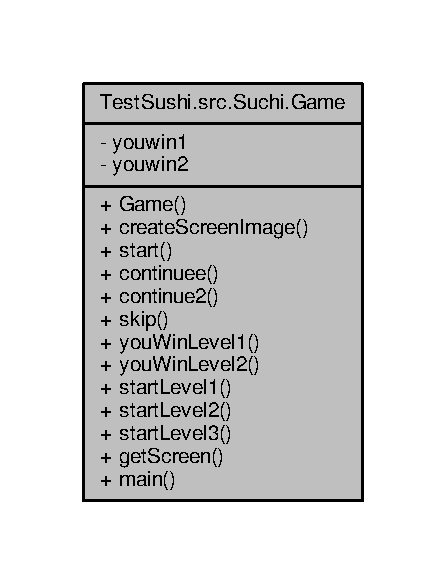
\includegraphics[width=214pt]{classTestSushi_1_1src_1_1Suchi_1_1Game__coll__graph}
\end{center}
\end{figure}
\subsubsection*{Fonctions membres publiques}
\begin{DoxyCompactItemize}
\item 
\hyperlink{classTestSushi_1_1src_1_1Suchi_1_1Game_a080b679d900a5355a58c87aa0e2be12a}{Game} (String url)
\begin{DoxyCompactList}\small\item\em Constructeur. \end{DoxyCompactList}\item 
void \hyperlink{classTestSushi_1_1src_1_1Suchi_1_1Game_a63c142c6be839eff06e2381962b43422}{create\+Screen\+Image} (Buffered\+Image image)
\begin{DoxyCompactList}\small\item\em Méthode qui crée l\textquotesingle{}image du screen au format png. \end{DoxyCompactList}\item 
void \hyperlink{classTestSushi_1_1src_1_1Suchi_1_1Game_a9083c7e4bb330ebd05de1ad90d0de345}{start} ()  throws A\+W\+T\+Exception, Interrupted\+Exception
\item 
void \hyperlink{classTestSushi_1_1src_1_1Suchi_1_1Game_a136917318745e2966eec3c102ef20f57}{continuee} ()  throws A\+W\+T\+Exception
\item 
void \hyperlink{classTestSushi_1_1src_1_1Suchi_1_1Game_a37b17625141098299b4c606bbde99664}{continue2} ()  throws A\+W\+T\+Exception
\item 
void \hyperlink{classTestSushi_1_1src_1_1Suchi_1_1Game_acfa2b3e1a2afb508fd9f5a2ea48880d4}{skip} ()  throws A\+W\+T\+Exception
\item 
boolean \hyperlink{classTestSushi_1_1src_1_1Suchi_1_1Game_a627e7f357a85a65408869c4928f0aaba}{you\+Win\+Level1} ()
\item 
boolean \hyperlink{classTestSushi_1_1src_1_1Suchi_1_1Game_a23b63ff8a5456156d556549f32c0ef5a}{you\+Win\+Level2} ()
\item 
void \hyperlink{classTestSushi_1_1src_1_1Suchi_1_1Game_afab54e5fed238f38957b72a6aa5364ff}{start\+Level1} (\hyperlink{classTestSushi_1_1src_1_1Suchi_1_1Game}{Game} g, \hyperlink{classTestSushi_1_1src_1_1Suchi_1_1Client}{Client} c)  throws A\+W\+T\+Exception, Interrupted\+Exception
\item 
void \hyperlink{classTestSushi_1_1src_1_1Suchi_1_1Game_a815c21a7f2cb47ebbcd9b400cebd16ae}{start\+Level2} (\hyperlink{classTestSushi_1_1src_1_1Suchi_1_1Game}{Game} g, \hyperlink{classTestSushi_1_1src_1_1Suchi_1_1Client}{Client} c)  throws A\+W\+T\+Exception, Interrupted\+Exception
\item 
void \hyperlink{classTestSushi_1_1src_1_1Suchi_1_1Game_a5e6bfc9bc7b59378669a811697bce2ca}{start\+Level3} (\hyperlink{classTestSushi_1_1src_1_1Suchi_1_1Game}{Game} g, \hyperlink{classTestSushi_1_1src_1_1Suchi_1_1Client}{Client} c)  throws A\+W\+T\+Exception, Interrupted\+Exception
\end{DoxyCompactItemize}
\subsubsection*{Fonctions membres publiques statiques}
\begin{DoxyCompactItemize}
\item 
static Buffered\+Image \hyperlink{classTestSushi_1_1src_1_1Suchi_1_1Game_aa813531009368ed875efd0c389e3e0f0}{get\+Screen} (int x)
\begin{DoxyCompactList}\small\item\em méthode qui prend un screen après x millisecondes \end{DoxyCompactList}\item 
static void \hyperlink{classTestSushi_1_1src_1_1Suchi_1_1Game_a480bc28787435229b94ae33334ec0e99}{main} (String\mbox{[}$\,$\mbox{]} args)  throws A\+W\+T\+Exception, Interrupted\+Exception 
\end{DoxyCompactItemize}
\subsubsection*{Attributs privés}
\begin{DoxyCompactItemize}
\item 
String \hyperlink{classTestSushi_1_1src_1_1Suchi_1_1Game_aaac6987e76afc5905150189e9e9b0638}{youwin1} = \char`\"{}sprites/youwin.\+png\char`\"{}
\item 
String \hyperlink{classTestSushi_1_1src_1_1Suchi_1_1Game_aca3e6d370eca4c7f5e9968998f87bce7}{youwin2} = \char`\"{}sprites/you\+Win2.\+png\char`\"{}
\end{DoxyCompactItemize}


\subsubsection{Documentation des constructeurs et destructeur}
\hypertarget{classTestSushi_1_1src_1_1Suchi_1_1Game_a080b679d900a5355a58c87aa0e2be12a}{}\index{Test\+Sushi\+::src\+::\+Suchi\+::\+Game@{Test\+Sushi\+::src\+::\+Suchi\+::\+Game}!Game@{Game}}
\index{Game@{Game}!Test\+Sushi\+::src\+::\+Suchi\+::\+Game@{Test\+Sushi\+::src\+::\+Suchi\+::\+Game}}
\paragraph[{Game}]{\setlength{\rightskip}{0pt plus 5cm}Test\+Sushi.\+src.\+Suchi.\+Game.\+Game (
\begin{DoxyParamCaption}
\item[{String}]{url}
\end{DoxyParamCaption}
)}\label{classTestSushi_1_1src_1_1Suchi_1_1Game_a080b679d900a5355a58c87aa0e2be12a}


Constructeur. 


\begin{DoxyParams}{Paramètres}
{\em url} & l\textquotesingle{}url du jeu \\
\hline
\end{DoxyParams}


Référencé par Test\+Sushi.\+src.\+Suchi.\+Game.\+main().



\subsubsection{Documentation des fonctions membres}
\hypertarget{classTestSushi_1_1src_1_1Suchi_1_1Game_a37b17625141098299b4c606bbde99664}{}\index{Test\+Sushi\+::src\+::\+Suchi\+::\+Game@{Test\+Sushi\+::src\+::\+Suchi\+::\+Game}!continue2@{continue2}}
\index{continue2@{continue2}!Test\+Sushi\+::src\+::\+Suchi\+::\+Game@{Test\+Sushi\+::src\+::\+Suchi\+::\+Game}}
\paragraph[{continue2}]{\setlength{\rightskip}{0pt plus 5cm}void Test\+Sushi.\+src.\+Suchi.\+Game.\+continue2 (
\begin{DoxyParamCaption}
{}
\end{DoxyParamCaption}
) throws A\+W\+T\+Exception}\label{classTestSushi_1_1src_1_1Suchi_1_1Game_a37b17625141098299b4c606bbde99664}

\begin{DoxyExceptions}{Exceptions}
{\em A\+W\+T\+Exception} & \\
\hline
\end{DoxyExceptions}
\hypertarget{classTestSushi_1_1src_1_1Suchi_1_1Game_a136917318745e2966eec3c102ef20f57}{}\index{Test\+Sushi\+::src\+::\+Suchi\+::\+Game@{Test\+Sushi\+::src\+::\+Suchi\+::\+Game}!continuee@{continuee}}
\index{continuee@{continuee}!Test\+Sushi\+::src\+::\+Suchi\+::\+Game@{Test\+Sushi\+::src\+::\+Suchi\+::\+Game}}
\paragraph[{continuee}]{\setlength{\rightskip}{0pt plus 5cm}void Test\+Sushi.\+src.\+Suchi.\+Game.\+continuee (
\begin{DoxyParamCaption}
{}
\end{DoxyParamCaption}
) throws A\+W\+T\+Exception}\label{classTestSushi_1_1src_1_1Suchi_1_1Game_a136917318745e2966eec3c102ef20f57}

\begin{DoxyExceptions}{Exceptions}
{\em A\+W\+T\+Exception} & \\
\hline
\end{DoxyExceptions}
\hypertarget{classTestSushi_1_1src_1_1Suchi_1_1Game_a63c142c6be839eff06e2381962b43422}{}\index{Test\+Sushi\+::src\+::\+Suchi\+::\+Game@{Test\+Sushi\+::src\+::\+Suchi\+::\+Game}!create\+Screen\+Image@{create\+Screen\+Image}}
\index{create\+Screen\+Image@{create\+Screen\+Image}!Test\+Sushi\+::src\+::\+Suchi\+::\+Game@{Test\+Sushi\+::src\+::\+Suchi\+::\+Game}}
\paragraph[{create\+Screen\+Image}]{\setlength{\rightskip}{0pt plus 5cm}void Test\+Sushi.\+src.\+Suchi.\+Game.\+create\+Screen\+Image (
\begin{DoxyParamCaption}
\item[{Buffered\+Image}]{image}
\end{DoxyParamCaption}
)}\label{classTestSushi_1_1src_1_1Suchi_1_1Game_a63c142c6be839eff06e2381962b43422}


Méthode qui crée l\textquotesingle{}image du screen au format png. 


\begin{DoxyParams}{Paramètres}
{\em image} & Un Buffered\+Image a sauvegardé \\
\hline
\end{DoxyParams}
\hypertarget{classTestSushi_1_1src_1_1Suchi_1_1Game_aa813531009368ed875efd0c389e3e0f0}{}\index{Test\+Sushi\+::src\+::\+Suchi\+::\+Game@{Test\+Sushi\+::src\+::\+Suchi\+::\+Game}!get\+Screen@{get\+Screen}}
\index{get\+Screen@{get\+Screen}!Test\+Sushi\+::src\+::\+Suchi\+::\+Game@{Test\+Sushi\+::src\+::\+Suchi\+::\+Game}}
\paragraph[{get\+Screen}]{\setlength{\rightskip}{0pt plus 5cm}static Buffered\+Image Test\+Sushi.\+src.\+Suchi.\+Game.\+get\+Screen (
\begin{DoxyParamCaption}
\item[{int}]{x}
\end{DoxyParamCaption}
)\hspace{0.3cm}{\ttfamily [static]}}\label{classTestSushi_1_1src_1_1Suchi_1_1Game_aa813531009368ed875efd0c389e3e0f0}


méthode qui prend un screen après x millisecondes 


\begin{DoxyParams}{Paramètres}
{\em x} & le temps de délai en millisecondes \\
\hline
\end{DoxyParams}
\begin{DoxyReturn}{Renvoie}
l\textquotesingle{}image de la zone de jeu déjà cadré 
\end{DoxyReturn}


Référencé par Test\+Sushi.\+src.\+Suchi.\+Recette.\+buy\+Noori(), Test\+Sushi.\+src.\+Suchi.\+Recette.\+buy\+Rice(), Test\+Sushi.\+src.\+Suchi.\+Recette.\+buy\+Roe(), Test\+Sushi.\+src.\+Suchi.\+Recette.\+buy\+Salmon(), Test\+Sushi.\+src.\+Suchi.\+Recette.\+buy\+Shrimp(), Test\+Sushi.\+src.\+Suchi.\+Screen\+Capture\+Rectangle.\+main(), Test\+Sushi.\+src.\+Suchi.\+Game.\+you\+Win\+Level1(), et Test\+Sushi.\+src.\+Suchi.\+Game.\+you\+Win\+Level2().

\hypertarget{classTestSushi_1_1src_1_1Suchi_1_1Game_a480bc28787435229b94ae33334ec0e99}{}\index{Test\+Sushi\+::src\+::\+Suchi\+::\+Game@{Test\+Sushi\+::src\+::\+Suchi\+::\+Game}!main@{main}}
\index{main@{main}!Test\+Sushi\+::src\+::\+Suchi\+::\+Game@{Test\+Sushi\+::src\+::\+Suchi\+::\+Game}}
\paragraph[{main}]{\setlength{\rightskip}{0pt plus 5cm}static void Test\+Sushi.\+src.\+Suchi.\+Game.\+main (
\begin{DoxyParamCaption}
\item[{String\mbox{[}$\,$\mbox{]}}]{args}
\end{DoxyParamCaption}
) throws A\+W\+T\+Exception, Interrupted\+Exception\hspace{0.3cm}{\ttfamily [static]}}\label{classTestSushi_1_1src_1_1Suchi_1_1Game_a480bc28787435229b94ae33334ec0e99}
\hypertarget{classTestSushi_1_1src_1_1Suchi_1_1Game_acfa2b3e1a2afb508fd9f5a2ea48880d4}{}\index{Test\+Sushi\+::src\+::\+Suchi\+::\+Game@{Test\+Sushi\+::src\+::\+Suchi\+::\+Game}!skip@{skip}}
\index{skip@{skip}!Test\+Sushi\+::src\+::\+Suchi\+::\+Game@{Test\+Sushi\+::src\+::\+Suchi\+::\+Game}}
\paragraph[{skip}]{\setlength{\rightskip}{0pt plus 5cm}void Test\+Sushi.\+src.\+Suchi.\+Game.\+skip (
\begin{DoxyParamCaption}
{}
\end{DoxyParamCaption}
) throws A\+W\+T\+Exception}\label{classTestSushi_1_1src_1_1Suchi_1_1Game_acfa2b3e1a2afb508fd9f5a2ea48880d4}

\begin{DoxyExceptions}{Exceptions}
{\em A\+W\+T\+Exception} & \\
\hline
\end{DoxyExceptions}
\hypertarget{classTestSushi_1_1src_1_1Suchi_1_1Game_a9083c7e4bb330ebd05de1ad90d0de345}{}\index{Test\+Sushi\+::src\+::\+Suchi\+::\+Game@{Test\+Sushi\+::src\+::\+Suchi\+::\+Game}!start@{start}}
\index{start@{start}!Test\+Sushi\+::src\+::\+Suchi\+::\+Game@{Test\+Sushi\+::src\+::\+Suchi\+::\+Game}}
\paragraph[{start}]{\setlength{\rightskip}{0pt plus 5cm}void Test\+Sushi.\+src.\+Suchi.\+Game.\+start (
\begin{DoxyParamCaption}
{}
\end{DoxyParamCaption}
) throws A\+W\+T\+Exception, Interrupted\+Exception}\label{classTestSushi_1_1src_1_1Suchi_1_1Game_a9083c7e4bb330ebd05de1ad90d0de345}

\begin{DoxyExceptions}{Exceptions}
{\em A\+W\+T\+Exception} & \\
\hline
{\em Interrupted\+Exception} & \\
\hline
\end{DoxyExceptions}
\hypertarget{classTestSushi_1_1src_1_1Suchi_1_1Game_afab54e5fed238f38957b72a6aa5364ff}{}\index{Test\+Sushi\+::src\+::\+Suchi\+::\+Game@{Test\+Sushi\+::src\+::\+Suchi\+::\+Game}!start\+Level1@{start\+Level1}}
\index{start\+Level1@{start\+Level1}!Test\+Sushi\+::src\+::\+Suchi\+::\+Game@{Test\+Sushi\+::src\+::\+Suchi\+::\+Game}}
\paragraph[{start\+Level1}]{\setlength{\rightskip}{0pt plus 5cm}void Test\+Sushi.\+src.\+Suchi.\+Game.\+start\+Level1 (
\begin{DoxyParamCaption}
\item[{{\bf Game}}]{g, }
\item[{{\bf Client}}]{c}
\end{DoxyParamCaption}
) throws A\+W\+T\+Exception, Interrupted\+Exception}\label{classTestSushi_1_1src_1_1Suchi_1_1Game_afab54e5fed238f38957b72a6aa5364ff}

\begin{DoxyParams}{Paramètres}
{\em g} & \\
\hline
{\em c} & \\
\hline
\end{DoxyParams}

\begin{DoxyExceptions}{Exceptions}
{\em A\+W\+T\+Exception} & \\
\hline
{\em Interrupted\+Exception} & \\
\hline
\end{DoxyExceptions}


Référencé par Test\+Sushi.\+src.\+Suchi.\+Game.\+main().

\hypertarget{classTestSushi_1_1src_1_1Suchi_1_1Game_a815c21a7f2cb47ebbcd9b400cebd16ae}{}\index{Test\+Sushi\+::src\+::\+Suchi\+::\+Game@{Test\+Sushi\+::src\+::\+Suchi\+::\+Game}!start\+Level2@{start\+Level2}}
\index{start\+Level2@{start\+Level2}!Test\+Sushi\+::src\+::\+Suchi\+::\+Game@{Test\+Sushi\+::src\+::\+Suchi\+::\+Game}}
\paragraph[{start\+Level2}]{\setlength{\rightskip}{0pt plus 5cm}void Test\+Sushi.\+src.\+Suchi.\+Game.\+start\+Level2 (
\begin{DoxyParamCaption}
\item[{{\bf Game}}]{g, }
\item[{{\bf Client}}]{c}
\end{DoxyParamCaption}
) throws A\+W\+T\+Exception, Interrupted\+Exception}\label{classTestSushi_1_1src_1_1Suchi_1_1Game_a815c21a7f2cb47ebbcd9b400cebd16ae}

\begin{DoxyParams}{Paramètres}
{\em g} & \\
\hline
{\em c} & \\
\hline
\end{DoxyParams}

\begin{DoxyExceptions}{Exceptions}
{\em A\+W\+T\+Exception} & \\
\hline
{\em Interrupted\+Exception} & \\
\hline
\end{DoxyExceptions}


Référencé par Test\+Sushi.\+src.\+Suchi.\+Game.\+main().

\hypertarget{classTestSushi_1_1src_1_1Suchi_1_1Game_a5e6bfc9bc7b59378669a811697bce2ca}{}\index{Test\+Sushi\+::src\+::\+Suchi\+::\+Game@{Test\+Sushi\+::src\+::\+Suchi\+::\+Game}!start\+Level3@{start\+Level3}}
\index{start\+Level3@{start\+Level3}!Test\+Sushi\+::src\+::\+Suchi\+::\+Game@{Test\+Sushi\+::src\+::\+Suchi\+::\+Game}}
\paragraph[{start\+Level3}]{\setlength{\rightskip}{0pt plus 5cm}void Test\+Sushi.\+src.\+Suchi.\+Game.\+start\+Level3 (
\begin{DoxyParamCaption}
\item[{{\bf Game}}]{g, }
\item[{{\bf Client}}]{c}
\end{DoxyParamCaption}
) throws A\+W\+T\+Exception, Interrupted\+Exception}\label{classTestSushi_1_1src_1_1Suchi_1_1Game_a5e6bfc9bc7b59378669a811697bce2ca}

\begin{DoxyParams}{Paramètres}
{\em g} & \\
\hline
{\em c} & \\
\hline
\end{DoxyParams}

\begin{DoxyExceptions}{Exceptions}
{\em A\+W\+T\+Exception} & \\
\hline
{\em Interrupted\+Exception} & \\
\hline
\end{DoxyExceptions}


Référencé par Test\+Sushi.\+src.\+Suchi.\+Game.\+main().

\hypertarget{classTestSushi_1_1src_1_1Suchi_1_1Game_a627e7f357a85a65408869c4928f0aaba}{}\index{Test\+Sushi\+::src\+::\+Suchi\+::\+Game@{Test\+Sushi\+::src\+::\+Suchi\+::\+Game}!you\+Win\+Level1@{you\+Win\+Level1}}
\index{you\+Win\+Level1@{you\+Win\+Level1}!Test\+Sushi\+::src\+::\+Suchi\+::\+Game@{Test\+Sushi\+::src\+::\+Suchi\+::\+Game}}
\paragraph[{you\+Win\+Level1}]{\setlength{\rightskip}{0pt plus 5cm}boolean Test\+Sushi.\+src.\+Suchi.\+Game.\+you\+Win\+Level1 (
\begin{DoxyParamCaption}
{}
\end{DoxyParamCaption}
)}\label{classTestSushi_1_1src_1_1Suchi_1_1Game_a627e7f357a85a65408869c4928f0aaba}
\begin{DoxyReturn}{Renvoie}

\end{DoxyReturn}
\hypertarget{classTestSushi_1_1src_1_1Suchi_1_1Game_a23b63ff8a5456156d556549f32c0ef5a}{}\index{Test\+Sushi\+::src\+::\+Suchi\+::\+Game@{Test\+Sushi\+::src\+::\+Suchi\+::\+Game}!you\+Win\+Level2@{you\+Win\+Level2}}
\index{you\+Win\+Level2@{you\+Win\+Level2}!Test\+Sushi\+::src\+::\+Suchi\+::\+Game@{Test\+Sushi\+::src\+::\+Suchi\+::\+Game}}
\paragraph[{you\+Win\+Level2}]{\setlength{\rightskip}{0pt plus 5cm}boolean Test\+Sushi.\+src.\+Suchi.\+Game.\+you\+Win\+Level2 (
\begin{DoxyParamCaption}
{}
\end{DoxyParamCaption}
)}\label{classTestSushi_1_1src_1_1Suchi_1_1Game_a23b63ff8a5456156d556549f32c0ef5a}
\begin{DoxyReturn}{Renvoie}

\end{DoxyReturn}


\subsubsection{Documentation des données membres}
\hypertarget{classTestSushi_1_1src_1_1Suchi_1_1Game_aaac6987e76afc5905150189e9e9b0638}{}\index{Test\+Sushi\+::src\+::\+Suchi\+::\+Game@{Test\+Sushi\+::src\+::\+Suchi\+::\+Game}!youwin1@{youwin1}}
\index{youwin1@{youwin1}!Test\+Sushi\+::src\+::\+Suchi\+::\+Game@{Test\+Sushi\+::src\+::\+Suchi\+::\+Game}}
\paragraph[{youwin1}]{\setlength{\rightskip}{0pt plus 5cm}String Test\+Sushi.\+src.\+Suchi.\+Game.\+youwin1 = \char`\"{}sprites/youwin.\+png\char`\"{}\hspace{0.3cm}{\ttfamily [private]}}\label{classTestSushi_1_1src_1_1Suchi_1_1Game_aaac6987e76afc5905150189e9e9b0638}


Référencé par Test\+Sushi.\+src.\+Suchi.\+Game.\+you\+Win\+Level1().

\hypertarget{classTestSushi_1_1src_1_1Suchi_1_1Game_aca3e6d370eca4c7f5e9968998f87bce7}{}\index{Test\+Sushi\+::src\+::\+Suchi\+::\+Game@{Test\+Sushi\+::src\+::\+Suchi\+::\+Game}!youwin2@{youwin2}}
\index{youwin2@{youwin2}!Test\+Sushi\+::src\+::\+Suchi\+::\+Game@{Test\+Sushi\+::src\+::\+Suchi\+::\+Game}}
\paragraph[{youwin2}]{\setlength{\rightskip}{0pt plus 5cm}String Test\+Sushi.\+src.\+Suchi.\+Game.\+youwin2 = \char`\"{}sprites/you\+Win2.\+png\char`\"{}\hspace{0.3cm}{\ttfamily [private]}}\label{classTestSushi_1_1src_1_1Suchi_1_1Game_aca3e6d370eca4c7f5e9968998f87bce7}


Référencé par Test\+Sushi.\+src.\+Suchi.\+Game.\+you\+Win\+Level2().



La documentation de cette classe a été générée à partir du fichier suivant \+:\begin{DoxyCompactItemize}
\item 
\hyperlink{projet_2TestSushi_2src_2Suchi_2Game_8java}{projet/\+Test\+Sushi/src/\+Suchi/\+Game.\+java}\end{DoxyCompactItemize}

\hypertarget{classSuchi_1_1Game}{}\subsection{Référence de la classe Suchi.\+Game}
\label{classSuchi_1_1Game}\index{Suchi.\+Game@{Suchi.\+Game}}


Graphe de collaboration de Suchi.\+Game\+:\nopagebreak
\begin{figure}[H]
\begin{center}
\leavevmode
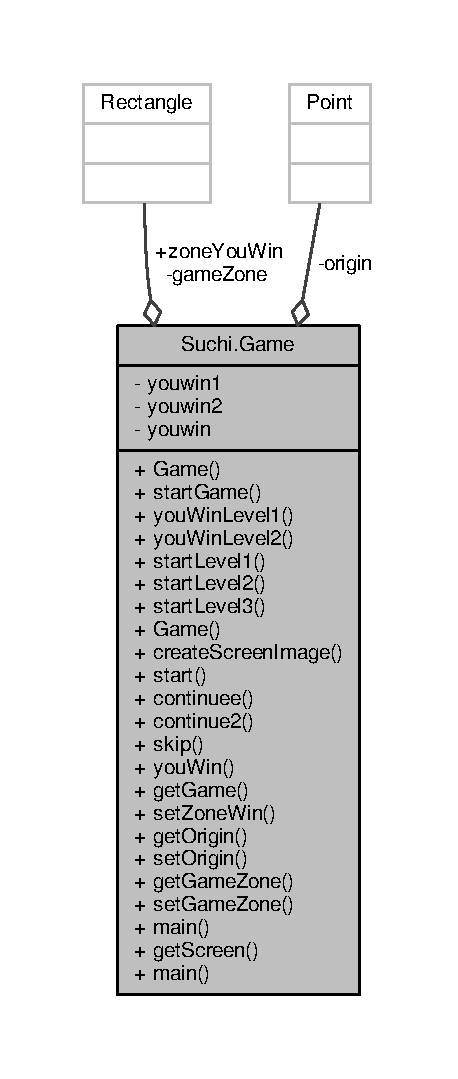
\includegraphics[width=220pt]{classSuchi_1_1Game__coll__graph}
\end{center}
\end{figure}
\subsubsection*{Fonctions membres publiques}
\begin{DoxyCompactItemize}
\item 
\hyperlink{classSuchi_1_1Game_a552ba6ea99b0ac919c41cf7f866b9a75}{Game} (String url)
\begin{DoxyCompactList}\small\item\em Constructeur. \end{DoxyCompactList}\item 
void \hyperlink{classSuchi_1_1Game_abee3ad7bb5a48f2a1f8d653698feb5f6}{start\+Game} ()  throws Exception
\item 
boolean \hyperlink{classSuchi_1_1Game_a297ea3b6be73823136d0bf3610e7c1ac}{you\+Win\+Level1} ()  throws A\+W\+T\+Exception
\item 
boolean \hyperlink{classSuchi_1_1Game_ab2d524572b556014055a7d4169001841}{you\+Win\+Level2} ()  throws A\+W\+T\+Exception
\item 
void \hyperlink{classSuchi_1_1Game_aeddc35c515b0d76f030efdbe1beb82db}{start\+Level1} (\hyperlink{classSuchi_1_1Client}{Client} c)  throws Exception
\item 
void \hyperlink{classSuchi_1_1Game_a8158842b22cc4e8c17e6b4085d9b5665}{start\+Level2} (\hyperlink{classSuchi_1_1Client}{Client} c)  throws Exception
\item 
void \hyperlink{classSuchi_1_1Game_a143479f6385bb267c7ee6059d80624fb}{start\+Level3} (\hyperlink{classSuchi_1_1Client}{Client} c)  throws Exception
\item 
\hyperlink{classSuchi_1_1Game_a552ba6ea99b0ac919c41cf7f866b9a75}{Game} (String url)
\item 
void \hyperlink{classSuchi_1_1Game_ad0a068c884bd0e250e92fb421c1c0763}{create\+Screen\+Image} (Buffered\+Image image)
\item 
void \hyperlink{classSuchi_1_1Game_ac7626fe6860eb60c2991524534d969dd}{start} ()  throws A\+W\+T\+Exception, Interrupted\+Exception
\item 
void \hyperlink{classSuchi_1_1Game_ad59775ca365f2a0e732be88411eaa255}{continuee} ()  throws A\+W\+T\+Exception
\item 
void \hyperlink{classSuchi_1_1Game_a0683a178cefd9d35a0eea5e4bbeeae78}{continue2} ()  throws A\+W\+T\+Exception
\item 
void \hyperlink{classSuchi_1_1Game_a12cde13afba4bf934886ce65fdc82b48}{skip} ()  throws A\+W\+T\+Exception
\item 
boolean \hyperlink{classSuchi_1_1Game_a3f4b5cfd1b51a2859cd9f51798d6966b}{you\+Win} ()
\item 
\hyperlink{classSuchi_1_1Game}{Game} \hyperlink{classSuchi_1_1Game_aea29c2bb6d69690cb5ff393473de8a9f}{get\+Game} ()
\end{DoxyCompactItemize}
\subsubsection*{Fonctions membres publiques statiques}
\begin{DoxyCompactItemize}
\item 
static void \hyperlink{classSuchi_1_1Game_ae9281ba8129a421e5d9607fc5eb5b41b}{set\+Zone\+Win} ()
\item 
static Point \hyperlink{classSuchi_1_1Game_a44d83961cd9bd6e93e8a21bd2865d49d}{get\+Origin} ()
\item 
static void \hyperlink{classSuchi_1_1Game_adf6b2ce5a22c42201a840fb0560b76f8}{set\+Origin} (Point new\+Origin)
\item 
static Rectangle \hyperlink{classSuchi_1_1Game_a73f030fa4f2c33ab3eb297423ff7a653}{get\+Game\+Zone} ()
\item 
static void \hyperlink{classSuchi_1_1Game_af37a4c12dd370a9b2865eb3cf667155e}{set\+Game\+Zone} (Rectangle new\+Game\+Zone)
\item 
static void \hyperlink{classSuchi_1_1Game_ab791d29f0d1d51ffb369a47c5def6ded}{main} (String\mbox{[}$\,$\mbox{]}args)
\item 
static Buffered\+Image \hyperlink{classSuchi_1_1Game_af0783e5007b8544ae5bba0cb78af3fb9}{get\+Screen} (int x)
\item 
static void \hyperlink{classSuchi_1_1Game_a4d54c6aa1bfad6d6203cd1f6a6096851}{main} (String\mbox{[}$\,$\mbox{]} args)  throws A\+W\+T\+Exception, Interrupted\+Exception 
\end{DoxyCompactItemize}
\subsubsection*{Attributs publics statiques}
\begin{DoxyCompactItemize}
\item 
static Rectangle \hyperlink{classSuchi_1_1Game_a2d7d0ec84563aca4b9eb88e861cefabe}{zone\+You\+Win}
\end{DoxyCompactItemize}
\subsubsection*{Attributs privés}
\begin{DoxyCompactItemize}
\item 
String \hyperlink{classSuchi_1_1Game_ae96d9d4f7dfa76d515cd059fa78884e8}{youwin1} = \char`\"{}sprites/youwin.\+png\char`\"{}
\item 
String \hyperlink{classSuchi_1_1Game_addb638e2316b9b72f74483db82eda767}{youwin2} = \char`\"{}sprites/youwin.\+png\char`\"{}
\item 
String \hyperlink{classSuchi_1_1Game_ac376917f0f8c62cd49134c459c61fd2c}{youwin} = \char`\"{}Sprites/youwin.\+png\char`\"{}
\end{DoxyCompactItemize}
\subsubsection*{Attributs privés statiques}
\begin{DoxyCompactItemize}
\item 
static Point \hyperlink{classSuchi_1_1Game_a9b3921f82615ebbd22a71a3334ba48db}{origin}
\item 
static Rectangle \hyperlink{classSuchi_1_1Game_a6beaeaaa0a1075d9420693dda0620d12}{game\+Zone}
\end{DoxyCompactItemize}


\subsubsection{Documentation des constructeurs et destructeur}
\hypertarget{classSuchi_1_1Game_a552ba6ea99b0ac919c41cf7f866b9a75}{}\index{Suchi\+::\+Game@{Suchi\+::\+Game}!Game@{Game}}
\index{Game@{Game}!Suchi\+::\+Game@{Suchi\+::\+Game}}
\paragraph[{Game}]{\setlength{\rightskip}{0pt plus 5cm}Suchi.\+Game.\+Game (
\begin{DoxyParamCaption}
\item[{String}]{url}
\end{DoxyParamCaption}
)}\label{classSuchi_1_1Game_a552ba6ea99b0ac919c41cf7f866b9a75}


Constructeur. 

Point d\textquotesingle{}entrée du programme, nécessite l\textquotesingle{}url du jeu à jouer 
\begin{DoxyParams}{Paramètres}
{\em url} & U\+R\+L du jeu à jouer \\
\hline
\end{DoxyParams}


Référencé par Suchi.\+Game.\+main().

\hypertarget{classSuchi_1_1Game_a552ba6ea99b0ac919c41cf7f866b9a75}{}\index{Suchi\+::\+Game@{Suchi\+::\+Game}!Game@{Game}}
\index{Game@{Game}!Suchi\+::\+Game@{Suchi\+::\+Game}}
\paragraph[{Game}]{\setlength{\rightskip}{0pt plus 5cm}Suchi.\+Game.\+Game (
\begin{DoxyParamCaption}
\item[{String}]{url}
\end{DoxyParamCaption}
)}\label{classSuchi_1_1Game_a552ba6ea99b0ac919c41cf7f866b9a75}


\subsubsection{Documentation des fonctions membres}
\hypertarget{classSuchi_1_1Game_a0683a178cefd9d35a0eea5e4bbeeae78}{}\index{Suchi\+::\+Game@{Suchi\+::\+Game}!continue2@{continue2}}
\index{continue2@{continue2}!Suchi\+::\+Game@{Suchi\+::\+Game}}
\paragraph[{continue2}]{\setlength{\rightskip}{0pt plus 5cm}void Suchi.\+Game.\+continue2 (
\begin{DoxyParamCaption}
{}
\end{DoxyParamCaption}
) throws A\+W\+T\+Exception}\label{classSuchi_1_1Game_a0683a178cefd9d35a0eea5e4bbeeae78}
\hypertarget{classSuchi_1_1Game_ad59775ca365f2a0e732be88411eaa255}{}\index{Suchi\+::\+Game@{Suchi\+::\+Game}!continuee@{continuee}}
\index{continuee@{continuee}!Suchi\+::\+Game@{Suchi\+::\+Game}}
\paragraph[{continuee}]{\setlength{\rightskip}{0pt plus 5cm}void Suchi.\+Game.\+continuee (
\begin{DoxyParamCaption}
{}
\end{DoxyParamCaption}
) throws A\+W\+T\+Exception}\label{classSuchi_1_1Game_ad59775ca365f2a0e732be88411eaa255}
\hypertarget{classSuchi_1_1Game_ad0a068c884bd0e250e92fb421c1c0763}{}\index{Suchi\+::\+Game@{Suchi\+::\+Game}!create\+Screen\+Image@{create\+Screen\+Image}}
\index{create\+Screen\+Image@{create\+Screen\+Image}!Suchi\+::\+Game@{Suchi\+::\+Game}}
\paragraph[{create\+Screen\+Image}]{\setlength{\rightskip}{0pt plus 5cm}void Suchi.\+Game.\+create\+Screen\+Image (
\begin{DoxyParamCaption}
\item[{Buffered\+Image}]{image}
\end{DoxyParamCaption}
)}\label{classSuchi_1_1Game_ad0a068c884bd0e250e92fb421c1c0763}
\hypertarget{classSuchi_1_1Game_aea29c2bb6d69690cb5ff393473de8a9f}{}\index{Suchi\+::\+Game@{Suchi\+::\+Game}!get\+Game@{get\+Game}}
\index{get\+Game@{get\+Game}!Suchi\+::\+Game@{Suchi\+::\+Game}}
\paragraph[{get\+Game}]{\setlength{\rightskip}{0pt plus 5cm}{\bf Game} Suchi.\+Game.\+get\+Game (
\begin{DoxyParamCaption}
{}
\end{DoxyParamCaption}
)}\label{classSuchi_1_1Game_aea29c2bb6d69690cb5ff393473de8a9f}
\hypertarget{classSuchi_1_1Game_a73f030fa4f2c33ab3eb297423ff7a653}{}\index{Suchi\+::\+Game@{Suchi\+::\+Game}!get\+Game\+Zone@{get\+Game\+Zone}}
\index{get\+Game\+Zone@{get\+Game\+Zone}!Suchi\+::\+Game@{Suchi\+::\+Game}}
\paragraph[{get\+Game\+Zone}]{\setlength{\rightskip}{0pt plus 5cm}static Rectangle Suchi.\+Game.\+get\+Game\+Zone (
\begin{DoxyParamCaption}
{}
\end{DoxyParamCaption}
)\hspace{0.3cm}{\ttfamily [static]}}\label{classSuchi_1_1Game_a73f030fa4f2c33ab3eb297423ff7a653}
\begin{DoxyReturn}{Renvoie}

\end{DoxyReturn}


Référencé par Suchi.\+Ia.\+Ia(), et Pictures.\+Recon.\+Recon().

\hypertarget{classSuchi_1_1Game_a44d83961cd9bd6e93e8a21bd2865d49d}{}\index{Suchi\+::\+Game@{Suchi\+::\+Game}!get\+Origin@{get\+Origin}}
\index{get\+Origin@{get\+Origin}!Suchi\+::\+Game@{Suchi\+::\+Game}}
\paragraph[{get\+Origin}]{\setlength{\rightskip}{0pt plus 5cm}static Point Suchi.\+Game.\+get\+Origin (
\begin{DoxyParamCaption}
{}
\end{DoxyParamCaption}
)\hspace{0.3cm}{\ttfamily [static]}}\label{classSuchi_1_1Game_a44d83961cd9bd6e93e8a21bd2865d49d}
\begin{DoxyReturn}{Renvoie}

\end{DoxyReturn}


Référencé par Suchi.\+Dot.\+translate().

\hypertarget{classSuchi_1_1Game_af0783e5007b8544ae5bba0cb78af3fb9}{}\index{Suchi\+::\+Game@{Suchi\+::\+Game}!get\+Screen@{get\+Screen}}
\index{get\+Screen@{get\+Screen}!Suchi\+::\+Game@{Suchi\+::\+Game}}
\paragraph[{get\+Screen}]{\setlength{\rightskip}{0pt plus 5cm}static Buffered\+Image Suchi.\+Game.\+get\+Screen (
\begin{DoxyParamCaption}
\item[{int}]{x}
\end{DoxyParamCaption}
)\hspace{0.3cm}{\ttfamily [static]}}\label{classSuchi_1_1Game_af0783e5007b8544ae5bba0cb78af3fb9}


Référencé par Suchi.\+Screen\+Capture\+Rectangle.\+main(), et Suchi.\+Game.\+you\+Win().

\hypertarget{classSuchi_1_1Game_a4d54c6aa1bfad6d6203cd1f6a6096851}{}\index{Suchi\+::\+Game@{Suchi\+::\+Game}!main@{main}}
\index{main@{main}!Suchi\+::\+Game@{Suchi\+::\+Game}}
\paragraph[{main}]{\setlength{\rightskip}{0pt plus 5cm}static void Suchi.\+Game.\+main (
\begin{DoxyParamCaption}
\item[{String\mbox{[}$\,$\mbox{]}}]{args}
\end{DoxyParamCaption}
) throws A\+W\+T\+Exception, Interrupted\+Exception\hspace{0.3cm}{\ttfamily [static]}}\label{classSuchi_1_1Game_a4d54c6aa1bfad6d6203cd1f6a6096851}
\hypertarget{classSuchi_1_1Game_ab791d29f0d1d51ffb369a47c5def6ded}{}\index{Suchi\+::\+Game@{Suchi\+::\+Game}!main@{main}}
\index{main@{main}!Suchi\+::\+Game@{Suchi\+::\+Game}}
\paragraph[{main}]{\setlength{\rightskip}{0pt plus 5cm}static void Suchi.\+Game.\+main (
\begin{DoxyParamCaption}
\item[{String\mbox{[}$\,$\mbox{]}}]{args}
\end{DoxyParamCaption}
)\hspace{0.3cm}{\ttfamily [static]}}\label{classSuchi_1_1Game_ab791d29f0d1d51ffb369a47c5def6ded}
\hypertarget{classSuchi_1_1Game_af37a4c12dd370a9b2865eb3cf667155e}{}\index{Suchi\+::\+Game@{Suchi\+::\+Game}!set\+Game\+Zone@{set\+Game\+Zone}}
\index{set\+Game\+Zone@{set\+Game\+Zone}!Suchi\+::\+Game@{Suchi\+::\+Game}}
\paragraph[{set\+Game\+Zone}]{\setlength{\rightskip}{0pt plus 5cm}static void Suchi.\+Game.\+set\+Game\+Zone (
\begin{DoxyParamCaption}
\item[{Rectangle}]{new\+Game\+Zone}
\end{DoxyParamCaption}
)\hspace{0.3cm}{\ttfamily [static]}}\label{classSuchi_1_1Game_af37a4c12dd370a9b2865eb3cf667155e}

\begin{DoxyParams}{Paramètres}
{\em new\+Game\+Zone} & \\
\hline
\end{DoxyParams}


Référencé par Suchi.\+Toolbox.\+detect\+Game\+Zone().

\hypertarget{classSuchi_1_1Game_adf6b2ce5a22c42201a840fb0560b76f8}{}\index{Suchi\+::\+Game@{Suchi\+::\+Game}!set\+Origin@{set\+Origin}}
\index{set\+Origin@{set\+Origin}!Suchi\+::\+Game@{Suchi\+::\+Game}}
\paragraph[{set\+Origin}]{\setlength{\rightskip}{0pt plus 5cm}static void Suchi.\+Game.\+set\+Origin (
\begin{DoxyParamCaption}
\item[{Point}]{new\+Origin}
\end{DoxyParamCaption}
)\hspace{0.3cm}{\ttfamily [static]}}\label{classSuchi_1_1Game_adf6b2ce5a22c42201a840fb0560b76f8}

\begin{DoxyParams}{Paramètres}
{\em new\+Origin} & \\
\hline
\end{DoxyParams}


Référencé par Suchi.\+Toolbox.\+detect\+Game\+Zone().

\hypertarget{classSuchi_1_1Game_ae9281ba8129a421e5d9607fc5eb5b41b}{}\index{Suchi\+::\+Game@{Suchi\+::\+Game}!set\+Zone\+Win@{set\+Zone\+Win}}
\index{set\+Zone\+Win@{set\+Zone\+Win}!Suchi\+::\+Game@{Suchi\+::\+Game}}
\paragraph[{set\+Zone\+Win}]{\setlength{\rightskip}{0pt plus 5cm}static void Suchi.\+Game.\+set\+Zone\+Win (
\begin{DoxyParamCaption}
{}
\end{DoxyParamCaption}
)\hspace{0.3cm}{\ttfamily [static]}}\label{classSuchi_1_1Game_ae9281ba8129a421e5d9607fc5eb5b41b}
\hypertarget{classSuchi_1_1Game_a12cde13afba4bf934886ce65fdc82b48}{}\index{Suchi\+::\+Game@{Suchi\+::\+Game}!skip@{skip}}
\index{skip@{skip}!Suchi\+::\+Game@{Suchi\+::\+Game}}
\paragraph[{skip}]{\setlength{\rightskip}{0pt plus 5cm}void Suchi.\+Game.\+skip (
\begin{DoxyParamCaption}
{}
\end{DoxyParamCaption}
) throws A\+W\+T\+Exception}\label{classSuchi_1_1Game_a12cde13afba4bf934886ce65fdc82b48}
\hypertarget{classSuchi_1_1Game_ac7626fe6860eb60c2991524534d969dd}{}\index{Suchi\+::\+Game@{Suchi\+::\+Game}!start@{start}}
\index{start@{start}!Suchi\+::\+Game@{Suchi\+::\+Game}}
\paragraph[{start}]{\setlength{\rightskip}{0pt plus 5cm}void Suchi.\+Game.\+start (
\begin{DoxyParamCaption}
{}
\end{DoxyParamCaption}
) throws A\+W\+T\+Exception, Interrupted\+Exception}\label{classSuchi_1_1Game_ac7626fe6860eb60c2991524534d969dd}
\hypertarget{classSuchi_1_1Game_abee3ad7bb5a48f2a1f8d653698feb5f6}{}\index{Suchi\+::\+Game@{Suchi\+::\+Game}!start\+Game@{start\+Game}}
\index{start\+Game@{start\+Game}!Suchi\+::\+Game@{Suchi\+::\+Game}}
\paragraph[{start\+Game}]{\setlength{\rightskip}{0pt plus 5cm}void Suchi.\+Game.\+start\+Game (
\begin{DoxyParamCaption}
{}
\end{DoxyParamCaption}
) throws Exception}\label{classSuchi_1_1Game_abee3ad7bb5a48f2a1f8d653698feb5f6}

\begin{DoxyExceptions}{Exceptions}
{\em Exception} & \\
\hline
\end{DoxyExceptions}


Référencé par Suchi.\+Game.\+start\+Level1().

\hypertarget{classSuchi_1_1Game_aeddc35c515b0d76f030efdbe1beb82db}{}\index{Suchi\+::\+Game@{Suchi\+::\+Game}!start\+Level1@{start\+Level1}}
\index{start\+Level1@{start\+Level1}!Suchi\+::\+Game@{Suchi\+::\+Game}}
\paragraph[{start\+Level1}]{\setlength{\rightskip}{0pt plus 5cm}void Suchi.\+Game.\+start\+Level1 (
\begin{DoxyParamCaption}
\item[{{\bf Client}}]{c}
\end{DoxyParamCaption}
) throws Exception}\label{classSuchi_1_1Game_aeddc35c515b0d76f030efdbe1beb82db}

\begin{DoxyParams}{Paramètres}
{\em c} & \\
\hline
\end{DoxyParams}

\begin{DoxyExceptions}{Exceptions}
{\em Exception} & \\
\hline
\end{DoxyExceptions}


Référencé par Suchi.\+Toolbox.\+game\+Routine().

\hypertarget{classSuchi_1_1Game_a8158842b22cc4e8c17e6b4085d9b5665}{}\index{Suchi\+::\+Game@{Suchi\+::\+Game}!start\+Level2@{start\+Level2}}
\index{start\+Level2@{start\+Level2}!Suchi\+::\+Game@{Suchi\+::\+Game}}
\paragraph[{start\+Level2}]{\setlength{\rightskip}{0pt plus 5cm}void Suchi.\+Game.\+start\+Level2 (
\begin{DoxyParamCaption}
\item[{{\bf Client}}]{c}
\end{DoxyParamCaption}
) throws Exception}\label{classSuchi_1_1Game_a8158842b22cc4e8c17e6b4085d9b5665}

\begin{DoxyParams}{Paramètres}
{\em c} & \\
\hline
\end{DoxyParams}

\begin{DoxyExceptions}{Exceptions}
{\em Exception} & \\
\hline
\end{DoxyExceptions}


Référencé par Suchi.\+Toolbox.\+game\+Routine().

\hypertarget{classSuchi_1_1Game_a143479f6385bb267c7ee6059d80624fb}{}\index{Suchi\+::\+Game@{Suchi\+::\+Game}!start\+Level3@{start\+Level3}}
\index{start\+Level3@{start\+Level3}!Suchi\+::\+Game@{Suchi\+::\+Game}}
\paragraph[{start\+Level3}]{\setlength{\rightskip}{0pt plus 5cm}void Suchi.\+Game.\+start\+Level3 (
\begin{DoxyParamCaption}
\item[{{\bf Client}}]{c}
\end{DoxyParamCaption}
) throws Exception}\label{classSuchi_1_1Game_a143479f6385bb267c7ee6059d80624fb}

\begin{DoxyParams}{Paramètres}
{\em c} & \\
\hline
\end{DoxyParams}

\begin{DoxyExceptions}{Exceptions}
{\em Exception} & \\
\hline
\end{DoxyExceptions}


Référencé par Suchi.\+Toolbox.\+game\+Routine().

\hypertarget{classSuchi_1_1Game_a3f4b5cfd1b51a2859cd9f51798d6966b}{}\index{Suchi\+::\+Game@{Suchi\+::\+Game}!you\+Win@{you\+Win}}
\index{you\+Win@{you\+Win}!Suchi\+::\+Game@{Suchi\+::\+Game}}
\paragraph[{you\+Win}]{\setlength{\rightskip}{0pt plus 5cm}boolean Suchi.\+Game.\+you\+Win (
\begin{DoxyParamCaption}
{}
\end{DoxyParamCaption}
)}\label{classSuchi_1_1Game_a3f4b5cfd1b51a2859cd9f51798d6966b}
\hypertarget{classSuchi_1_1Game_a297ea3b6be73823136d0bf3610e7c1ac}{}\index{Suchi\+::\+Game@{Suchi\+::\+Game}!you\+Win\+Level1@{you\+Win\+Level1}}
\index{you\+Win\+Level1@{you\+Win\+Level1}!Suchi\+::\+Game@{Suchi\+::\+Game}}
\paragraph[{you\+Win\+Level1}]{\setlength{\rightskip}{0pt plus 5cm}boolean Suchi.\+Game.\+you\+Win\+Level1 (
\begin{DoxyParamCaption}
{}
\end{DoxyParamCaption}
) throws A\+W\+T\+Exception}\label{classSuchi_1_1Game_a297ea3b6be73823136d0bf3610e7c1ac}
\begin{DoxyReturn}{Renvoie}

\end{DoxyReturn}

\begin{DoxyExceptions}{Exceptions}
{\em A\+W\+T\+Exception} & \\
\hline
\end{DoxyExceptions}


Référencé par Suchi.\+Game.\+start\+Level1().

\hypertarget{classSuchi_1_1Game_ab2d524572b556014055a7d4169001841}{}\index{Suchi\+::\+Game@{Suchi\+::\+Game}!you\+Win\+Level2@{you\+Win\+Level2}}
\index{you\+Win\+Level2@{you\+Win\+Level2}!Suchi\+::\+Game@{Suchi\+::\+Game}}
\paragraph[{you\+Win\+Level2}]{\setlength{\rightskip}{0pt plus 5cm}boolean Suchi.\+Game.\+you\+Win\+Level2 (
\begin{DoxyParamCaption}
{}
\end{DoxyParamCaption}
) throws A\+W\+T\+Exception}\label{classSuchi_1_1Game_ab2d524572b556014055a7d4169001841}
\begin{DoxyReturn}{Renvoie}

\end{DoxyReturn}

\begin{DoxyExceptions}{Exceptions}
{\em A\+W\+T\+Exception} & \\
\hline
\end{DoxyExceptions}


Référencé par Suchi.\+Game.\+start\+Level2(), et Suchi.\+Game.\+start\+Level3().



\subsubsection{Documentation des données membres}
\hypertarget{classSuchi_1_1Game_a6beaeaaa0a1075d9420693dda0620d12}{}\index{Suchi\+::\+Game@{Suchi\+::\+Game}!game\+Zone@{game\+Zone}}
\index{game\+Zone@{game\+Zone}!Suchi\+::\+Game@{Suchi\+::\+Game}}
\paragraph[{game\+Zone}]{\setlength{\rightskip}{0pt plus 5cm}Rectangle Suchi.\+Game.\+game\+Zone\hspace{0.3cm}{\ttfamily [static]}, {\ttfamily [private]}}\label{classSuchi_1_1Game_a6beaeaaa0a1075d9420693dda0620d12}


Référencé par Suchi.\+Game.\+get\+Game\+Zone().

\hypertarget{classSuchi_1_1Game_a9b3921f82615ebbd22a71a3334ba48db}{}\index{Suchi\+::\+Game@{Suchi\+::\+Game}!origin@{origin}}
\index{origin@{origin}!Suchi\+::\+Game@{Suchi\+::\+Game}}
\paragraph[{origin}]{\setlength{\rightskip}{0pt plus 5cm}Point Suchi.\+Game.\+origin\hspace{0.3cm}{\ttfamily [static]}, {\ttfamily [private]}}\label{classSuchi_1_1Game_a9b3921f82615ebbd22a71a3334ba48db}


Référencé par Suchi.\+Game.\+get\+Origin().

\hypertarget{classSuchi_1_1Game_ac376917f0f8c62cd49134c459c61fd2c}{}\index{Suchi\+::\+Game@{Suchi\+::\+Game}!youwin@{youwin}}
\index{youwin@{youwin}!Suchi\+::\+Game@{Suchi\+::\+Game}}
\paragraph[{youwin}]{\setlength{\rightskip}{0pt plus 5cm}String Suchi.\+Game.\+youwin = \char`\"{}Sprites/youwin.\+png\char`\"{}\hspace{0.3cm}{\ttfamily [private]}}\label{classSuchi_1_1Game_ac376917f0f8c62cd49134c459c61fd2c}
\hypertarget{classSuchi_1_1Game_ae96d9d4f7dfa76d515cd059fa78884e8}{}\index{Suchi\+::\+Game@{Suchi\+::\+Game}!youwin1@{youwin1}}
\index{youwin1@{youwin1}!Suchi\+::\+Game@{Suchi\+::\+Game}}
\paragraph[{youwin1}]{\setlength{\rightskip}{0pt plus 5cm}String Suchi.\+Game.\+youwin1 = \char`\"{}sprites/youwin.\+png\char`\"{}\hspace{0.3cm}{\ttfamily [private]}}\label{classSuchi_1_1Game_ae96d9d4f7dfa76d515cd059fa78884e8}
\hypertarget{classSuchi_1_1Game_addb638e2316b9b72f74483db82eda767}{}\index{Suchi\+::\+Game@{Suchi\+::\+Game}!youwin2@{youwin2}}
\index{youwin2@{youwin2}!Suchi\+::\+Game@{Suchi\+::\+Game}}
\paragraph[{youwin2}]{\setlength{\rightskip}{0pt plus 5cm}String Suchi.\+Game.\+youwin2 = \char`\"{}sprites/youwin.\+png\char`\"{}\hspace{0.3cm}{\ttfamily [private]}}\label{classSuchi_1_1Game_addb638e2316b9b72f74483db82eda767}
\hypertarget{classSuchi_1_1Game_a2d7d0ec84563aca4b9eb88e861cefabe}{}\index{Suchi\+::\+Game@{Suchi\+::\+Game}!zone\+You\+Win@{zone\+You\+Win}}
\index{zone\+You\+Win@{zone\+You\+Win}!Suchi\+::\+Game@{Suchi\+::\+Game}}
\paragraph[{zone\+You\+Win}]{\setlength{\rightskip}{0pt plus 5cm}Rectangle Suchi.\+Game.\+zone\+You\+Win\hspace{0.3cm}{\ttfamily [static]}}\label{classSuchi_1_1Game_a2d7d0ec84563aca4b9eb88e861cefabe}


La documentation de cette classe a été générée à partir du fichier suivant \+:\begin{DoxyCompactItemize}
\item 
\hyperlink{BotSofRetapage_2src_2Suchi_2Game_8java}{Bot\+Sof\+Retapage/src/\+Suchi/\+Game.\+java}\end{DoxyCompactItemize}

\hypertarget{classSuchi_1_1GameArea}{}\subsection{Référence de la classe Suchi.\+Game\+Area}
\label{classSuchi_1_1GameArea}\index{Suchi.\+Game\+Area@{Suchi.\+Game\+Area}}


Graphe de collaboration de Suchi.\+Game\+Area\+:\nopagebreak
\begin{figure}[H]
\begin{center}
\leavevmode
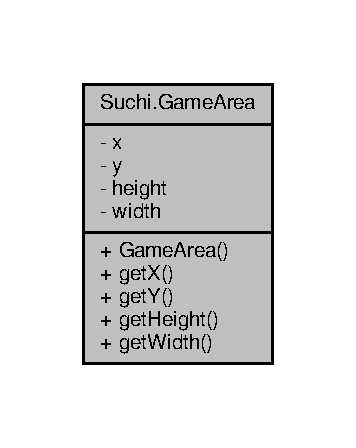
\includegraphics[width=171pt]{classSuchi_1_1GameArea__coll__graph}
\end{center}
\end{figure}
\subsubsection*{Fonctions membres publiques}
\begin{DoxyCompactItemize}
\item 
\hyperlink{classSuchi_1_1GameArea_a61c76bafee149d83259aea88df0c804e}{Game\+Area} (int \hyperlink{classSuchi_1_1GameArea_aa89bcaf59584201e5cdbf3006e33880b}{x}, int \hyperlink{classSuchi_1_1GameArea_a21715e2b105c4d602b0eabfa550d6e3a}{y}, int h, int w)
\item 
int \hyperlink{classSuchi_1_1GameArea_a598bf061ee493a40893f183fcbfc4be8}{get\+X} ()
\item 
int \hyperlink{classSuchi_1_1GameArea_adf21d825c56540c007bc97e7e484f41f}{get\+Y} ()
\item 
int \hyperlink{classSuchi_1_1GameArea_a9132a916eaeedc3e94c6365869833bde}{get\+Height} ()
\item 
int \hyperlink{classSuchi_1_1GameArea_aa821a0904266c1595e4f503995b7f8ac}{get\+Width} ()
\end{DoxyCompactItemize}
\subsubsection*{Attributs privés}
\begin{DoxyCompactItemize}
\item 
int \hyperlink{classSuchi_1_1GameArea_aa89bcaf59584201e5cdbf3006e33880b}{x}
\item 
int \hyperlink{classSuchi_1_1GameArea_a21715e2b105c4d602b0eabfa550d6e3a}{y}
\item 
int \hyperlink{classSuchi_1_1GameArea_a1b2fcf63587bc1c370a741151a67ff6d}{height}
\item 
int \hyperlink{classSuchi_1_1GameArea_ad959f934234c4765e29d8bf0291a04cc}{width}
\end{DoxyCompactItemize}


\subsubsection{Documentation des constructeurs et destructeur}
\hypertarget{classSuchi_1_1GameArea_a61c76bafee149d83259aea88df0c804e}{}\index{Suchi\+::\+Game\+Area@{Suchi\+::\+Game\+Area}!Game\+Area@{Game\+Area}}
\index{Game\+Area@{Game\+Area}!Suchi\+::\+Game\+Area@{Suchi\+::\+Game\+Area}}
\paragraph[{Game\+Area}]{\setlength{\rightskip}{0pt plus 5cm}Suchi.\+Game\+Area.\+Game\+Area (
\begin{DoxyParamCaption}
\item[{int}]{x, }
\item[{int}]{y, }
\item[{int}]{h, }
\item[{int}]{w}
\end{DoxyParamCaption}
)}\label{classSuchi_1_1GameArea_a61c76bafee149d83259aea88df0c804e}


\subsubsection{Documentation des fonctions membres}
\hypertarget{classSuchi_1_1GameArea_a9132a916eaeedc3e94c6365869833bde}{}\index{Suchi\+::\+Game\+Area@{Suchi\+::\+Game\+Area}!get\+Height@{get\+Height}}
\index{get\+Height@{get\+Height}!Suchi\+::\+Game\+Area@{Suchi\+::\+Game\+Area}}
\paragraph[{get\+Height}]{\setlength{\rightskip}{0pt plus 5cm}int Suchi.\+Game\+Area.\+get\+Height (
\begin{DoxyParamCaption}
{}
\end{DoxyParamCaption}
)}\label{classSuchi_1_1GameArea_a9132a916eaeedc3e94c6365869833bde}


Référencé par Suchi.\+Tool\+Box.\+Capture().

\hypertarget{classSuchi_1_1GameArea_aa821a0904266c1595e4f503995b7f8ac}{}\index{Suchi\+::\+Game\+Area@{Suchi\+::\+Game\+Area}!get\+Width@{get\+Width}}
\index{get\+Width@{get\+Width}!Suchi\+::\+Game\+Area@{Suchi\+::\+Game\+Area}}
\paragraph[{get\+Width}]{\setlength{\rightskip}{0pt plus 5cm}int Suchi.\+Game\+Area.\+get\+Width (
\begin{DoxyParamCaption}
{}
\end{DoxyParamCaption}
)}\label{classSuchi_1_1GameArea_aa821a0904266c1595e4f503995b7f8ac}


Référencé par Suchi.\+Tool\+Box.\+Capture().

\hypertarget{classSuchi_1_1GameArea_a598bf061ee493a40893f183fcbfc4be8}{}\index{Suchi\+::\+Game\+Area@{Suchi\+::\+Game\+Area}!get\+X@{get\+X}}
\index{get\+X@{get\+X}!Suchi\+::\+Game\+Area@{Suchi\+::\+Game\+Area}}
\paragraph[{get\+X}]{\setlength{\rightskip}{0pt plus 5cm}int Suchi.\+Game\+Area.\+get\+X (
\begin{DoxyParamCaption}
{}
\end{DoxyParamCaption}
)}\label{classSuchi_1_1GameArea_a598bf061ee493a40893f183fcbfc4be8}


Référencé par Suchi.\+Tool\+Box.\+Capture().

\hypertarget{classSuchi_1_1GameArea_adf21d825c56540c007bc97e7e484f41f}{}\index{Suchi\+::\+Game\+Area@{Suchi\+::\+Game\+Area}!get\+Y@{get\+Y}}
\index{get\+Y@{get\+Y}!Suchi\+::\+Game\+Area@{Suchi\+::\+Game\+Area}}
\paragraph[{get\+Y}]{\setlength{\rightskip}{0pt plus 5cm}int Suchi.\+Game\+Area.\+get\+Y (
\begin{DoxyParamCaption}
{}
\end{DoxyParamCaption}
)}\label{classSuchi_1_1GameArea_adf21d825c56540c007bc97e7e484f41f}


Référencé par Suchi.\+Tool\+Box.\+Capture().



\subsubsection{Documentation des données membres}
\hypertarget{classSuchi_1_1GameArea_a1b2fcf63587bc1c370a741151a67ff6d}{}\index{Suchi\+::\+Game\+Area@{Suchi\+::\+Game\+Area}!height@{height}}
\index{height@{height}!Suchi\+::\+Game\+Area@{Suchi\+::\+Game\+Area}}
\paragraph[{height}]{\setlength{\rightskip}{0pt plus 5cm}int Suchi.\+Game\+Area.\+height\hspace{0.3cm}{\ttfamily [private]}}\label{classSuchi_1_1GameArea_a1b2fcf63587bc1c370a741151a67ff6d}


Référencé par Suchi.\+Game\+Area.\+get\+Height().

\hypertarget{classSuchi_1_1GameArea_ad959f934234c4765e29d8bf0291a04cc}{}\index{Suchi\+::\+Game\+Area@{Suchi\+::\+Game\+Area}!width@{width}}
\index{width@{width}!Suchi\+::\+Game\+Area@{Suchi\+::\+Game\+Area}}
\paragraph[{width}]{\setlength{\rightskip}{0pt plus 5cm}int Suchi.\+Game\+Area.\+width\hspace{0.3cm}{\ttfamily [private]}}\label{classSuchi_1_1GameArea_ad959f934234c4765e29d8bf0291a04cc}


Référencé par Suchi.\+Game\+Area.\+get\+Width().

\hypertarget{classSuchi_1_1GameArea_aa89bcaf59584201e5cdbf3006e33880b}{}\index{Suchi\+::\+Game\+Area@{Suchi\+::\+Game\+Area}!x@{x}}
\index{x@{x}!Suchi\+::\+Game\+Area@{Suchi\+::\+Game\+Area}}
\paragraph[{x}]{\setlength{\rightskip}{0pt plus 5cm}int Suchi.\+Game\+Area.\+x\hspace{0.3cm}{\ttfamily [private]}}\label{classSuchi_1_1GameArea_aa89bcaf59584201e5cdbf3006e33880b}


Référencé par Suchi.\+Game\+Area.\+Game\+Area(), et Suchi.\+Game\+Area.\+get\+X().

\hypertarget{classSuchi_1_1GameArea_a21715e2b105c4d602b0eabfa550d6e3a}{}\index{Suchi\+::\+Game\+Area@{Suchi\+::\+Game\+Area}!y@{y}}
\index{y@{y}!Suchi\+::\+Game\+Area@{Suchi\+::\+Game\+Area}}
\paragraph[{y}]{\setlength{\rightskip}{0pt plus 5cm}int Suchi.\+Game\+Area.\+y\hspace{0.3cm}{\ttfamily [private]}}\label{classSuchi_1_1GameArea_a21715e2b105c4d602b0eabfa550d6e3a}


Référencé par Suchi.\+Game\+Area.\+Game\+Area(), et Suchi.\+Game\+Area.\+get\+Y().



La documentation de cette classe a été générée à partir du fichier suivant \+:\begin{DoxyCompactItemize}
\item 
\hyperlink{GameArea_8java}{Game\+Area.\+java}\end{DoxyCompactItemize}

\hypertarget{classGameWindow}{}\subsection{Référence de la classe Game\+Window}
\label{classGameWindow}\index{Game\+Window@{Game\+Window}}


Graphe de collaboration de Game\+Window\+:\nopagebreak
\begin{figure}[H]
\begin{center}
\leavevmode
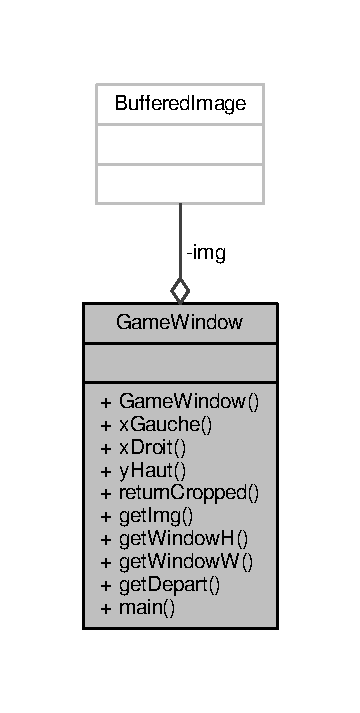
\includegraphics[width=173pt]{classGameWindow__coll__graph}
\end{center}
\end{figure}
\subsubsection*{Fonctions membres publiques}
\begin{DoxyCompactItemize}
\item 
\hyperlink{classGameWindow_aa10f854e7ec0e407a7bf776f126b4548}{Game\+Window} ()
\item 
int \hyperlink{classGameWindow_ad6e68a8aced99c138d607928bb9aaf82}{x\+Gauche} (Buffered\+Image \hyperlink{classGameWindow_a72d61cef747fc3a4b64d30078c833aed}{img})
\item 
int \hyperlink{classGameWindow_a7acbde7d0be4fb1e3db92f2eacaf5a94}{x\+Droit} (Buffered\+Image \hyperlink{classGameWindow_a72d61cef747fc3a4b64d30078c833aed}{img})
\item 
int \hyperlink{classGameWindow_a23ad629bc54c9a5c10189c881367b5f4}{y\+Haut} (Buffered\+Image \hyperlink{classGameWindow_a72d61cef747fc3a4b64d30078c833aed}{img})
\item 
Buffered\+Image \hyperlink{classGameWindow_ac2ecc4d61e2fb666c891ecd4c9d1cb08}{return\+Cropped} (Buffered\+Image \hyperlink{classGameWindow_a72d61cef747fc3a4b64d30078c833aed}{img})
\item 
Buffered\+Image \hyperlink{classGameWindow_acc4d41cfeb4eab5e593a3929ce654e69}{get\+Img} ()
\item 
int \hyperlink{classGameWindow_a8db0001a1a1974a36ea1e7c22e6a7e35}{get\+Window\+H} ()
\item 
int \hyperlink{classGameWindow_a28f716fe53f24acfe90fb7e4d71ba0a2}{get\+Window\+W} ()
\item 
Point \hyperlink{classGameWindow_aeb8312bfd2899bb35887df607208f972}{get\+Depart} ()
\end{DoxyCompactItemize}
\subsubsection*{Fonctions membres publiques statiques}
\begin{DoxyCompactItemize}
\item 
static void \hyperlink{classGameWindow_ab530b9757613a133cd94dffe4e51b462}{main} (String\mbox{[}$\,$\mbox{]} args)
\end{DoxyCompactItemize}
\subsubsection*{Attributs privés}
\begin{DoxyCompactItemize}
\item 
Buffered\+Image \hyperlink{classGameWindow_a72d61cef747fc3a4b64d30078c833aed}{img}
\end{DoxyCompactItemize}


\subsubsection{Documentation des constructeurs et destructeur}
\hypertarget{classGameWindow_aa10f854e7ec0e407a7bf776f126b4548}{}\index{Game\+Window@{Game\+Window}!Game\+Window@{Game\+Window}}
\index{Game\+Window@{Game\+Window}!Game\+Window@{Game\+Window}}
\paragraph[{Game\+Window}]{\setlength{\rightskip}{0pt plus 5cm}Game\+Window.\+Game\+Window (
\begin{DoxyParamCaption}
{}
\end{DoxyParamCaption}
)}\label{classGameWindow_aa10f854e7ec0e407a7bf776f126b4548}


\subsubsection{Documentation des fonctions membres}
\hypertarget{classGameWindow_aeb8312bfd2899bb35887df607208f972}{}\index{Game\+Window@{Game\+Window}!get\+Depart@{get\+Depart}}
\index{get\+Depart@{get\+Depart}!Game\+Window@{Game\+Window}}
\paragraph[{get\+Depart}]{\setlength{\rightskip}{0pt plus 5cm}Point Game\+Window.\+get\+Depart (
\begin{DoxyParamCaption}
{}
\end{DoxyParamCaption}
)}\label{classGameWindow_aeb8312bfd2899bb35887df607208f972}


Référencé par Clic\+Button.\+clique(), Clic\+Button.\+find\+X(), et Clic\+Button.\+find\+Y().

\hypertarget{classGameWindow_acc4d41cfeb4eab5e593a3929ce654e69}{}\index{Game\+Window@{Game\+Window}!get\+Img@{get\+Img}}
\index{get\+Img@{get\+Img}!Game\+Window@{Game\+Window}}
\paragraph[{get\+Img}]{\setlength{\rightskip}{0pt plus 5cm}Buffered\+Image Game\+Window.\+get\+Img (
\begin{DoxyParamCaption}
{}
\end{DoxyParamCaption}
)}\label{classGameWindow_acc4d41cfeb4eab5e593a3929ce654e69}
\hypertarget{classGameWindow_a8db0001a1a1974a36ea1e7c22e6a7e35}{}\index{Game\+Window@{Game\+Window}!get\+Window\+H@{get\+Window\+H}}
\index{get\+Window\+H@{get\+Window\+H}!Game\+Window@{Game\+Window}}
\paragraph[{get\+Window\+H}]{\setlength{\rightskip}{0pt plus 5cm}int Game\+Window.\+get\+Window\+H (
\begin{DoxyParamCaption}
{}
\end{DoxyParamCaption}
)}\label{classGameWindow_a8db0001a1a1974a36ea1e7c22e6a7e35}


Référencé par Clic\+Button.\+clique(), et Clic\+Button.\+find\+Y().

\hypertarget{classGameWindow_a28f716fe53f24acfe90fb7e4d71ba0a2}{}\index{Game\+Window@{Game\+Window}!get\+Window\+W@{get\+Window\+W}}
\index{get\+Window\+W@{get\+Window\+W}!Game\+Window@{Game\+Window}}
\paragraph[{get\+Window\+W}]{\setlength{\rightskip}{0pt plus 5cm}int Game\+Window.\+get\+Window\+W (
\begin{DoxyParamCaption}
{}
\end{DoxyParamCaption}
)}\label{classGameWindow_a28f716fe53f24acfe90fb7e4d71ba0a2}


Référencé par Clic\+Button.\+clique(), et Clic\+Button.\+find\+X().

\hypertarget{classGameWindow_ab530b9757613a133cd94dffe4e51b462}{}\index{Game\+Window@{Game\+Window}!main@{main}}
\index{main@{main}!Game\+Window@{Game\+Window}}
\paragraph[{main}]{\setlength{\rightskip}{0pt plus 5cm}static void Game\+Window.\+main (
\begin{DoxyParamCaption}
\item[{String\mbox{[}$\,$\mbox{]}}]{args}
\end{DoxyParamCaption}
)\hspace{0.3cm}{\ttfamily [static]}}\label{classGameWindow_ab530b9757613a133cd94dffe4e51b462}
\hypertarget{classGameWindow_ac2ecc4d61e2fb666c891ecd4c9d1cb08}{}\index{Game\+Window@{Game\+Window}!return\+Cropped@{return\+Cropped}}
\index{return\+Cropped@{return\+Cropped}!Game\+Window@{Game\+Window}}
\paragraph[{return\+Cropped}]{\setlength{\rightskip}{0pt plus 5cm}Buffered\+Image Game\+Window.\+return\+Cropped (
\begin{DoxyParamCaption}
\item[{Buffered\+Image}]{img}
\end{DoxyParamCaption}
)}\label{classGameWindow_ac2ecc4d61e2fb666c891ecd4c9d1cb08}
\hypertarget{classGameWindow_a7acbde7d0be4fb1e3db92f2eacaf5a94}{}\index{Game\+Window@{Game\+Window}!x\+Droit@{x\+Droit}}
\index{x\+Droit@{x\+Droit}!Game\+Window@{Game\+Window}}
\paragraph[{x\+Droit}]{\setlength{\rightskip}{0pt plus 5cm}int Game\+Window.\+x\+Droit (
\begin{DoxyParamCaption}
\item[{Buffered\+Image}]{img}
\end{DoxyParamCaption}
)}\label{classGameWindow_a7acbde7d0be4fb1e3db92f2eacaf5a94}


Référencé par get\+Window\+H(), get\+Window\+W(), et return\+Cropped().

\hypertarget{classGameWindow_ad6e68a8aced99c138d607928bb9aaf82}{}\index{Game\+Window@{Game\+Window}!x\+Gauche@{x\+Gauche}}
\index{x\+Gauche@{x\+Gauche}!Game\+Window@{Game\+Window}}
\paragraph[{x\+Gauche}]{\setlength{\rightskip}{0pt plus 5cm}int Game\+Window.\+x\+Gauche (
\begin{DoxyParamCaption}
\item[{Buffered\+Image}]{img}
\end{DoxyParamCaption}
)}\label{classGameWindow_ad6e68a8aced99c138d607928bb9aaf82}


Référencé par get\+Depart(), get\+Window\+H(), get\+Window\+W(), return\+Cropped(), et y\+Haut().

\hypertarget{classGameWindow_a23ad629bc54c9a5c10189c881367b5f4}{}\index{Game\+Window@{Game\+Window}!y\+Haut@{y\+Haut}}
\index{y\+Haut@{y\+Haut}!Game\+Window@{Game\+Window}}
\paragraph[{y\+Haut}]{\setlength{\rightskip}{0pt plus 5cm}int Game\+Window.\+y\+Haut (
\begin{DoxyParamCaption}
\item[{Buffered\+Image}]{img}
\end{DoxyParamCaption}
)}\label{classGameWindow_a23ad629bc54c9a5c10189c881367b5f4}


Référencé par get\+Depart(), et return\+Cropped().



\subsubsection{Documentation des données membres}
\hypertarget{classGameWindow_a72d61cef747fc3a4b64d30078c833aed}{}\index{Game\+Window@{Game\+Window}!img@{img}}
\index{img@{img}!Game\+Window@{Game\+Window}}
\paragraph[{img}]{\setlength{\rightskip}{0pt plus 5cm}Buffered\+Image Game\+Window.\+img\hspace{0.3cm}{\ttfamily [private]}}\label{classGameWindow_a72d61cef747fc3a4b64d30078c833aed}


Référencé par get\+Img().



La documentation de cette classe a été générée à partir du fichier suivant \+:\begin{DoxyCompactItemize}
\item 
\hyperlink{GameWindow_8java}{Game\+Window.\+java}\end{DoxyCompactItemize}

\hypertarget{classIA}{}\subsection{Référence de la classe I\+A}
\label{classIA}\index{I\+A@{I\+A}}


Graphe d\textquotesingle{}héritage de I\+A\+:\nopagebreak
\begin{figure}[H]
\begin{center}
\leavevmode
\includegraphics[height=550pt]{classIA__inherit__graph}
\end{center}
\end{figure}


Graphe de collaboration de I\+A\+:\nopagebreak
\begin{figure}[H]
\begin{center}
\leavevmode
\includegraphics[width=350pt]{classIA__coll__graph}
\end{center}
\end{figure}
\subsubsection*{Fonctions membres publiques}
\begin{DoxyCompactItemize}
\item 
\hyperlink{classIA_ac5567e7745fa95d02be55a502ba4eb54}{I\+A} (Rectangle rec)  throws A\+W\+T\+Exception 
\item 
void \hyperlink{classIA_af0e60d7ece7f50a3a7a5df8ca6c5d409}{click} (String zone)  throws A\+W\+T\+Exception, Interrupted\+Exception 
\item 
void \hyperlink{classIA_a0bf764584e254c4551de156962ae1e34}{initiate\+Game} ()  throws A\+W\+T\+Exception, Interrupted\+Exception 
\item 
\hyperlink{classZone}{Zone} \hyperlink{classIA_aa873ed13d9e2dc9572877397d6a02234}{get\+Zone} ()
\item 
void \hyperlink{classIA_a903fe1fd726b52cf01c1aa1e22320ae1}{save\+Sprites} ()  throws A\+W\+T\+Exception, I\+O\+Exception 
\item 
Array\+List$<$ Buffered\+Image $>$ \hyperlink{classIA_aa0afcde6a905b512450b54c1d7011732}{load\+Sprites} ()  throws A\+W\+T\+Exception 
\item 
String \hyperlink{classIA_a10fe21a4730bdf5d881225f8ab9a8c6f}{get\+Sushi} (Buffered\+Image sushi\+To\+Test)
\item 
void \hyperlink{classToolBox_a6e2363d41efa87ec225910f1665f04c9}{Capture} ()  throws A\+W\+T\+Exception 
\item 
void \hyperlink{classToolBox_a059e1404af5bcc5fbb1bb9dedfc20d66}{Capture\+Game} (int tps)  throws A\+W\+T\+Exception 
\item 
void \hyperlink{classToolBox_a84973bc465d7edad32f758829595c1da}{Launch} ()
\item 
void \hyperlink{classToolBox_aa0f5a8cb133c58a8d3ce98bc3e98d8ed}{Run} ()  throws Interrupted\+Exception, A\+W\+T\+Exception 
\item 
void \hyperlink{classToolBox_ad1cd486e0e4b502e023e0835638a9e0f}{Serve} ()  throws Interrupted\+Exception 
\item 
void \hyperlink{classToolBox_aa2c48c9b70735e54ed4123834ef9e5cf}{action\+Performed} (Action\+Event arg0)
\item 
void \hyperlink{classToolBox_ae3baa18f028039800f8c9fc07abf0931}{clic\+Bar} ()  throws A\+W\+T\+Exception, Interrupted\+Exception
\end{DoxyCompactItemize}
\subsubsection*{Attributs publics statiques}
\begin{DoxyCompactItemize}
\item 
static int \hyperlink{classIA_a7b2224d63b5c3c6f66456fa76d35ca17}{x\+Or}
\item 
static int \hyperlink{classIA_a715cc2f5ecfdcc10070efedae3ee1c1e}{y\+Or}
\item 
static Rectangle \hyperlink{classToolBox_a84023d6084fa90a7c5efb7802be85879}{ga}
\end{DoxyCompactItemize}
\subsubsection*{Attributs de paquetage}
\begin{DoxyCompactItemize}
\item 
Thread \hyperlink{classToolBox_a4a4a941d9d6b7892fab6299754098d16}{terminate}
\end{DoxyCompactItemize}
\subsubsection*{Attributs privés}
\begin{DoxyCompactItemize}
\item 
int \hyperlink{classIA_ab31d73d4297034d5a8fddc6ae1cd5c46}{width}
\item 
int \hyperlink{classIA_a96c12173b130e4e03d8bb75495bae440}{height}
\item 
\hyperlink{classZone}{Zone} \hyperlink{classIA_aaa96f9a826c59be2e231d020b05312d8}{zones}
\item 
\hyperlink{classReadZone}{Read\+Zone} \hyperlink{classIA_af8f75fc5120b869308190c66313e7139}{bulles}
\item 
Hash\+Map$<$ Buffered\+Image, String $>$ \hyperlink{classIA_abb06bcb730d01ee856e68c60c7c9539c}{sushi\+Reference}
\end{DoxyCompactItemize}
\subsubsection*{Attributs privés statiques}
\begin{DoxyCompactItemize}
\item 
static final long \hyperlink{classIA_a04d11d2607138e2a8edf27ca8d4ad23d}{serial\+Version\+U\+I\+D} = 5210558056865804594\+L
\item 
static int \hyperlink{classIA_aab9d3e69748c6640a5d56874a033c17d}{sprite\+Count} = 0
\end{DoxyCompactItemize}


\subsubsection{Documentation des constructeurs et destructeur}
\hypertarget{classIA_ac5567e7745fa95d02be55a502ba4eb54}{}\index{I\+A@{I\+A}!I\+A@{I\+A}}
\index{I\+A@{I\+A}!I\+A@{I\+A}}
\paragraph[{I\+A}]{\setlength{\rightskip}{0pt plus 5cm}I\+A.\+I\+A (
\begin{DoxyParamCaption}
\item[{Rectangle}]{rec}
\end{DoxyParamCaption}
) throws A\+W\+T\+Exception}\label{classIA_ac5567e7745fa95d02be55a502ba4eb54}


\subsubsection{Documentation des fonctions membres}
\hypertarget{classToolBox_aa2c48c9b70735e54ed4123834ef9e5cf}{}\index{I\+A@{I\+A}!action\+Performed@{action\+Performed}}
\index{action\+Performed@{action\+Performed}!I\+A@{I\+A}}
\paragraph[{action\+Performed}]{\setlength{\rightskip}{0pt plus 5cm}void Tool\+Box.\+action\+Performed (
\begin{DoxyParamCaption}
\item[{Action\+Event}]{arg0}
\end{DoxyParamCaption}
)\hspace{0.3cm}{\ttfamily [inherited]}}\label{classToolBox_aa2c48c9b70735e54ed4123834ef9e5cf}
\hypertarget{classToolBox_a6e2363d41efa87ec225910f1665f04c9}{}\index{I\+A@{I\+A}!Capture@{Capture}}
\index{Capture@{Capture}!I\+A@{I\+A}}
\paragraph[{Capture}]{\setlength{\rightskip}{0pt plus 5cm}void Tool\+Box.\+Capture (
\begin{DoxyParamCaption}
{}
\end{DoxyParamCaption}
) throws A\+W\+T\+Exception\hspace{0.3cm}{\ttfamily [inherited]}}\label{classToolBox_a6e2363d41efa87ec225910f1665f04c9}


Référencé par Tool\+Box.\+action\+Performed().

\hypertarget{classToolBox_a059e1404af5bcc5fbb1bb9dedfc20d66}{}\index{I\+A@{I\+A}!Capture\+Game@{Capture\+Game}}
\index{Capture\+Game@{Capture\+Game}!I\+A@{I\+A}}
\paragraph[{Capture\+Game}]{\setlength{\rightskip}{0pt plus 5cm}void Tool\+Box.\+Capture\+Game (
\begin{DoxyParamCaption}
\item[{int}]{tps}
\end{DoxyParamCaption}
) throws A\+W\+T\+Exception\hspace{0.3cm}{\ttfamily [inherited]}}\label{classToolBox_a059e1404af5bcc5fbb1bb9dedfc20d66}


Référencé par Tool\+Box.\+action\+Performed().

\hypertarget{classToolBox_ae3baa18f028039800f8c9fc07abf0931}{}\index{I\+A@{I\+A}!clic\+Bar@{clic\+Bar}}
\index{clic\+Bar@{clic\+Bar}!I\+A@{I\+A}}
\paragraph[{clic\+Bar}]{\setlength{\rightskip}{0pt plus 5cm}void Tool\+Box.\+clic\+Bar (
\begin{DoxyParamCaption}
{}
\end{DoxyParamCaption}
) throws A\+W\+T\+Exception, Interrupted\+Exception\hspace{0.3cm}{\ttfamily [inherited]}}\label{classToolBox_ae3baa18f028039800f8c9fc07abf0931}


Référencé par Tool\+Box.\+Serve().

\hypertarget{classIA_af0e60d7ece7f50a3a7a5df8ca6c5d409}{}\index{I\+A@{I\+A}!click@{click}}
\index{click@{click}!I\+A@{I\+A}}
\paragraph[{click}]{\setlength{\rightskip}{0pt plus 5cm}void I\+A.\+click (
\begin{DoxyParamCaption}
\item[{String}]{zone}
\end{DoxyParamCaption}
) throws A\+W\+T\+Exception, Interrupted\+Exception}\label{classIA_af0e60d7ece7f50a3a7a5df8ca6c5d409}


Référencé par Manager.\+buy\+Component(), initiate\+Game(), et Manager.\+make\+Sushi().

\hypertarget{classIA_a10fe21a4730bdf5d881225f8ab9a8c6f}{}\index{I\+A@{I\+A}!get\+Sushi@{get\+Sushi}}
\index{get\+Sushi@{get\+Sushi}!I\+A@{I\+A}}
\paragraph[{get\+Sushi}]{\setlength{\rightskip}{0pt plus 5cm}String I\+A.\+get\+Sushi (
\begin{DoxyParamCaption}
\item[{Buffered\+Image}]{sushi\+To\+Test}
\end{DoxyParamCaption}
)}\label{classIA_a10fe21a4730bdf5d881225f8ab9a8c6f}


Référencé par Manager.\+Check\+Bar().

\hypertarget{classIA_aa873ed13d9e2dc9572877397d6a02234}{}\index{I\+A@{I\+A}!get\+Zone@{get\+Zone}}
\index{get\+Zone@{get\+Zone}!I\+A@{I\+A}}
\paragraph[{get\+Zone}]{\setlength{\rightskip}{0pt plus 5cm}{\bf Zone} I\+A.\+get\+Zone (
\begin{DoxyParamCaption}
{}
\end{DoxyParamCaption}
)}\label{classIA_aa873ed13d9e2dc9572877397d6a02234}
\hypertarget{classIA_a0bf764584e254c4551de156962ae1e34}{}\index{I\+A@{I\+A}!initiate\+Game@{initiate\+Game}}
\index{initiate\+Game@{initiate\+Game}!I\+A@{I\+A}}
\paragraph[{initiate\+Game}]{\setlength{\rightskip}{0pt plus 5cm}void I\+A.\+initiate\+Game (
\begin{DoxyParamCaption}
{}
\end{DoxyParamCaption}
) throws A\+W\+T\+Exception, Interrupted\+Exception}\label{classIA_a0bf764584e254c4551de156962ae1e34}


Référencé par Tool\+Box.\+Run().

\hypertarget{classToolBox_a84973bc465d7edad32f758829595c1da}{}\index{I\+A@{I\+A}!Launch@{Launch}}
\index{Launch@{Launch}!I\+A@{I\+A}}
\paragraph[{Launch}]{\setlength{\rightskip}{0pt plus 5cm}void Tool\+Box.\+Launch (
\begin{DoxyParamCaption}
{}
\end{DoxyParamCaption}
)\hspace{0.3cm}{\ttfamily [inherited]}}\label{classToolBox_a84973bc465d7edad32f758829595c1da}


Référencé par Tool\+Box.\+action\+Performed().

\hypertarget{classIA_aa0afcde6a905b512450b54c1d7011732}{}\index{I\+A@{I\+A}!load\+Sprites@{load\+Sprites}}
\index{load\+Sprites@{load\+Sprites}!I\+A@{I\+A}}
\paragraph[{load\+Sprites}]{\setlength{\rightskip}{0pt plus 5cm}Array\+List$<$Buffered\+Image$>$ I\+A.\+load\+Sprites (
\begin{DoxyParamCaption}
{}
\end{DoxyParamCaption}
) throws A\+W\+T\+Exception}\label{classIA_aa0afcde6a905b512450b54c1d7011732}


Référencé par Manager.\+Check\+Bar().

\hypertarget{classToolBox_aa0f5a8cb133c58a8d3ce98bc3e98d8ed}{}\index{I\+A@{I\+A}!Run@{Run}}
\index{Run@{Run}!I\+A@{I\+A}}
\paragraph[{Run}]{\setlength{\rightskip}{0pt plus 5cm}void Tool\+Box.\+Run (
\begin{DoxyParamCaption}
{}
\end{DoxyParamCaption}
) throws Interrupted\+Exception, A\+W\+T\+Exception\hspace{0.3cm}{\ttfamily [inherited]}}\label{classToolBox_aa0f5a8cb133c58a8d3ce98bc3e98d8ed}


Référencé par Tool\+Box.\+action\+Performed().

\hypertarget{classIA_a903fe1fd726b52cf01c1aa1e22320ae1}{}\index{I\+A@{I\+A}!save\+Sprites@{save\+Sprites}}
\index{save\+Sprites@{save\+Sprites}!I\+A@{I\+A}}
\paragraph[{save\+Sprites}]{\setlength{\rightskip}{0pt plus 5cm}void I\+A.\+save\+Sprites (
\begin{DoxyParamCaption}
{}
\end{DoxyParamCaption}
) throws A\+W\+T\+Exception, I\+O\+Exception}\label{classIA_a903fe1fd726b52cf01c1aa1e22320ae1}


Référencé par Tool\+Box.\+action\+Performed().

\hypertarget{classToolBox_ad1cd486e0e4b502e023e0835638a9e0f}{}\index{I\+A@{I\+A}!Serve@{Serve}}
\index{Serve@{Serve}!I\+A@{I\+A}}
\paragraph[{Serve}]{\setlength{\rightskip}{0pt plus 5cm}void Tool\+Box.\+Serve (
\begin{DoxyParamCaption}
{}
\end{DoxyParamCaption}
) throws Interrupted\+Exception\hspace{0.3cm}{\ttfamily [inherited]}}\label{classToolBox_ad1cd486e0e4b502e023e0835638a9e0f}


Référencé par Tool\+Box.\+action\+Performed().



\subsubsection{Documentation des données membres}
\hypertarget{classIA_af8f75fc5120b869308190c66313e7139}{}\index{I\+A@{I\+A}!bulles@{bulles}}
\index{bulles@{bulles}!I\+A@{I\+A}}
\paragraph[{bulles}]{\setlength{\rightskip}{0pt plus 5cm}{\bf Read\+Zone} I\+A.\+bulles\hspace{0.3cm}{\ttfamily [private]}}\label{classIA_af8f75fc5120b869308190c66313e7139}
\hypertarget{classToolBox_a84023d6084fa90a7c5efb7802be85879}{}\index{I\+A@{I\+A}!ga@{ga}}
\index{ga@{ga}!I\+A@{I\+A}}
\paragraph[{ga}]{\setlength{\rightskip}{0pt plus 5cm}Rectangle Tool\+Box.\+ga\hspace{0.3cm}{\ttfamily [static]}, {\ttfamily [inherited]}}\label{classToolBox_a84023d6084fa90a7c5efb7802be85879}


Référencé par Manager.\+Manager().

\hypertarget{classIA_a96c12173b130e4e03d8bb75495bae440}{}\index{I\+A@{I\+A}!height@{height}}
\index{height@{height}!I\+A@{I\+A}}
\paragraph[{height}]{\setlength{\rightskip}{0pt plus 5cm}int I\+A.\+height\hspace{0.3cm}{\ttfamily [private]}}\label{classIA_a96c12173b130e4e03d8bb75495bae440}
\hypertarget{classIA_a04d11d2607138e2a8edf27ca8d4ad23d}{}\index{I\+A@{I\+A}!serial\+Version\+U\+I\+D@{serial\+Version\+U\+I\+D}}
\index{serial\+Version\+U\+I\+D@{serial\+Version\+U\+I\+D}!I\+A@{I\+A}}
\paragraph[{serial\+Version\+U\+I\+D}]{\setlength{\rightskip}{0pt plus 5cm}final long I\+A.\+serial\+Version\+U\+I\+D = 5210558056865804594\+L\hspace{0.3cm}{\ttfamily [static]}, {\ttfamily [private]}}\label{classIA_a04d11d2607138e2a8edf27ca8d4ad23d}
\hypertarget{classIA_aab9d3e69748c6640a5d56874a033c17d}{}\index{I\+A@{I\+A}!sprite\+Count@{sprite\+Count}}
\index{sprite\+Count@{sprite\+Count}!I\+A@{I\+A}}
\paragraph[{sprite\+Count}]{\setlength{\rightskip}{0pt plus 5cm}int I\+A.\+sprite\+Count = 0\hspace{0.3cm}{\ttfamily [static]}, {\ttfamily [private]}}\label{classIA_aab9d3e69748c6640a5d56874a033c17d}
\hypertarget{classIA_abb06bcb730d01ee856e68c60c7c9539c}{}\index{I\+A@{I\+A}!sushi\+Reference@{sushi\+Reference}}
\index{sushi\+Reference@{sushi\+Reference}!I\+A@{I\+A}}
\paragraph[{sushi\+Reference}]{\setlength{\rightskip}{0pt plus 5cm}Hash\+Map$<$Buffered\+Image, String$>$ I\+A.\+sushi\+Reference\hspace{0.3cm}{\ttfamily [private]}}\label{classIA_abb06bcb730d01ee856e68c60c7c9539c}
\hypertarget{classToolBox_a4a4a941d9d6b7892fab6299754098d16}{}\index{I\+A@{I\+A}!terminate@{terminate}}
\index{terminate@{terminate}!I\+A@{I\+A}}
\paragraph[{terminate}]{\setlength{\rightskip}{0pt plus 5cm}Thread Tool\+Box.\+terminate\hspace{0.3cm}{\ttfamily [package]}, {\ttfamily [inherited]}}\label{classToolBox_a4a4a941d9d6b7892fab6299754098d16}
\hypertarget{classIA_ab31d73d4297034d5a8fddc6ae1cd5c46}{}\index{I\+A@{I\+A}!width@{width}}
\index{width@{width}!I\+A@{I\+A}}
\paragraph[{width}]{\setlength{\rightskip}{0pt plus 5cm}int I\+A.\+width\hspace{0.3cm}{\ttfamily [private]}}\label{classIA_ab31d73d4297034d5a8fddc6ae1cd5c46}
\hypertarget{classIA_a7b2224d63b5c3c6f66456fa76d35ca17}{}\index{I\+A@{I\+A}!x\+Or@{x\+Or}}
\index{x\+Or@{x\+Or}!I\+A@{I\+A}}
\paragraph[{x\+Or}]{\setlength{\rightskip}{0pt plus 5cm}int I\+A.\+x\+Or\hspace{0.3cm}{\ttfamily [static]}}\label{classIA_a7b2224d63b5c3c6f66456fa76d35ca17}


Référencé par Dot.\+translate().

\hypertarget{classIA_a715cc2f5ecfdcc10070efedae3ee1c1e}{}\index{I\+A@{I\+A}!y\+Or@{y\+Or}}
\index{y\+Or@{y\+Or}!I\+A@{I\+A}}
\paragraph[{y\+Or}]{\setlength{\rightskip}{0pt plus 5cm}int I\+A.\+y\+Or\hspace{0.3cm}{\ttfamily [static]}}\label{classIA_a715cc2f5ecfdcc10070efedae3ee1c1e}


Référencé par Dot.\+translate().

\hypertarget{classIA_aaa96f9a826c59be2e231d020b05312d8}{}\index{I\+A@{I\+A}!zones@{zones}}
\index{zones@{zones}!I\+A@{I\+A}}
\paragraph[{zones}]{\setlength{\rightskip}{0pt plus 5cm}{\bf Zone} I\+A.\+zones\hspace{0.3cm}{\ttfamily [private]}}\label{classIA_aaa96f9a826c59be2e231d020b05312d8}


Référencé par get\+Zone().



La documentation de cette classe a été générée à partir du fichier suivant \+:\begin{DoxyCompactItemize}
\item 
\hyperlink{oldCode_2IA_8java}{old\+Code/\+I\+A.\+java}\end{DoxyCompactItemize}

\hypertarget{classmain_1_1IA}{}\subsection{Référence de la classe main.\+I\+A}
\label{classmain_1_1IA}\index{main.\+I\+A@{main.\+I\+A}}


Graphe d\textquotesingle{}héritage de main.\+I\+A\+:\nopagebreak
\begin{figure}[H]
\begin{center}
\leavevmode
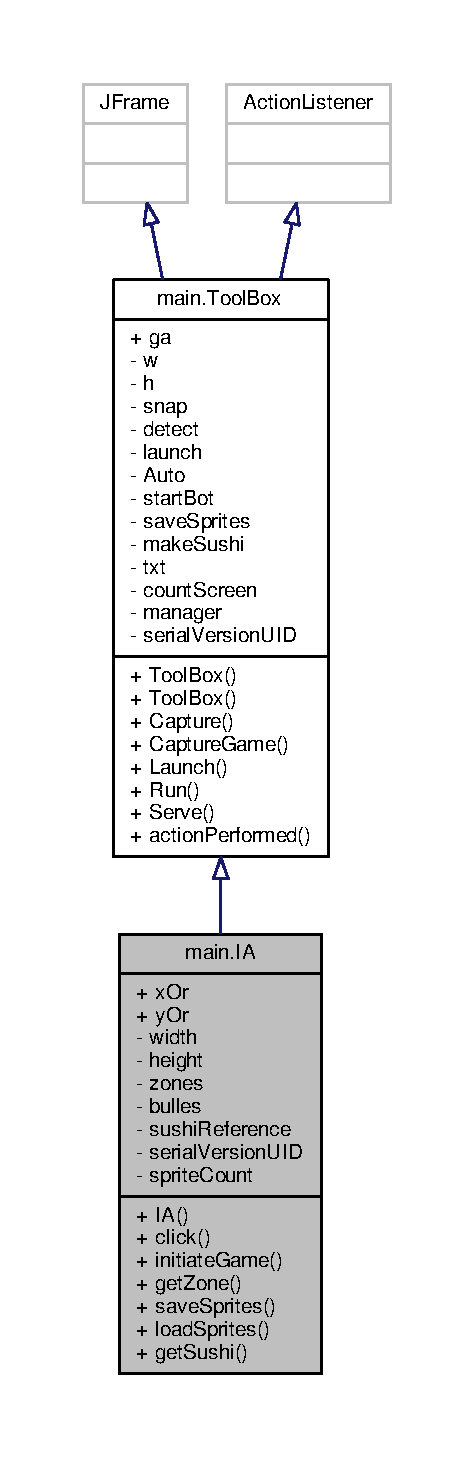
\includegraphics[height=550pt]{classmain_1_1IA__inherit__graph}
\end{center}
\end{figure}


Graphe de collaboration de main.\+I\+A\+:\nopagebreak
\begin{figure}[H]
\begin{center}
\leavevmode
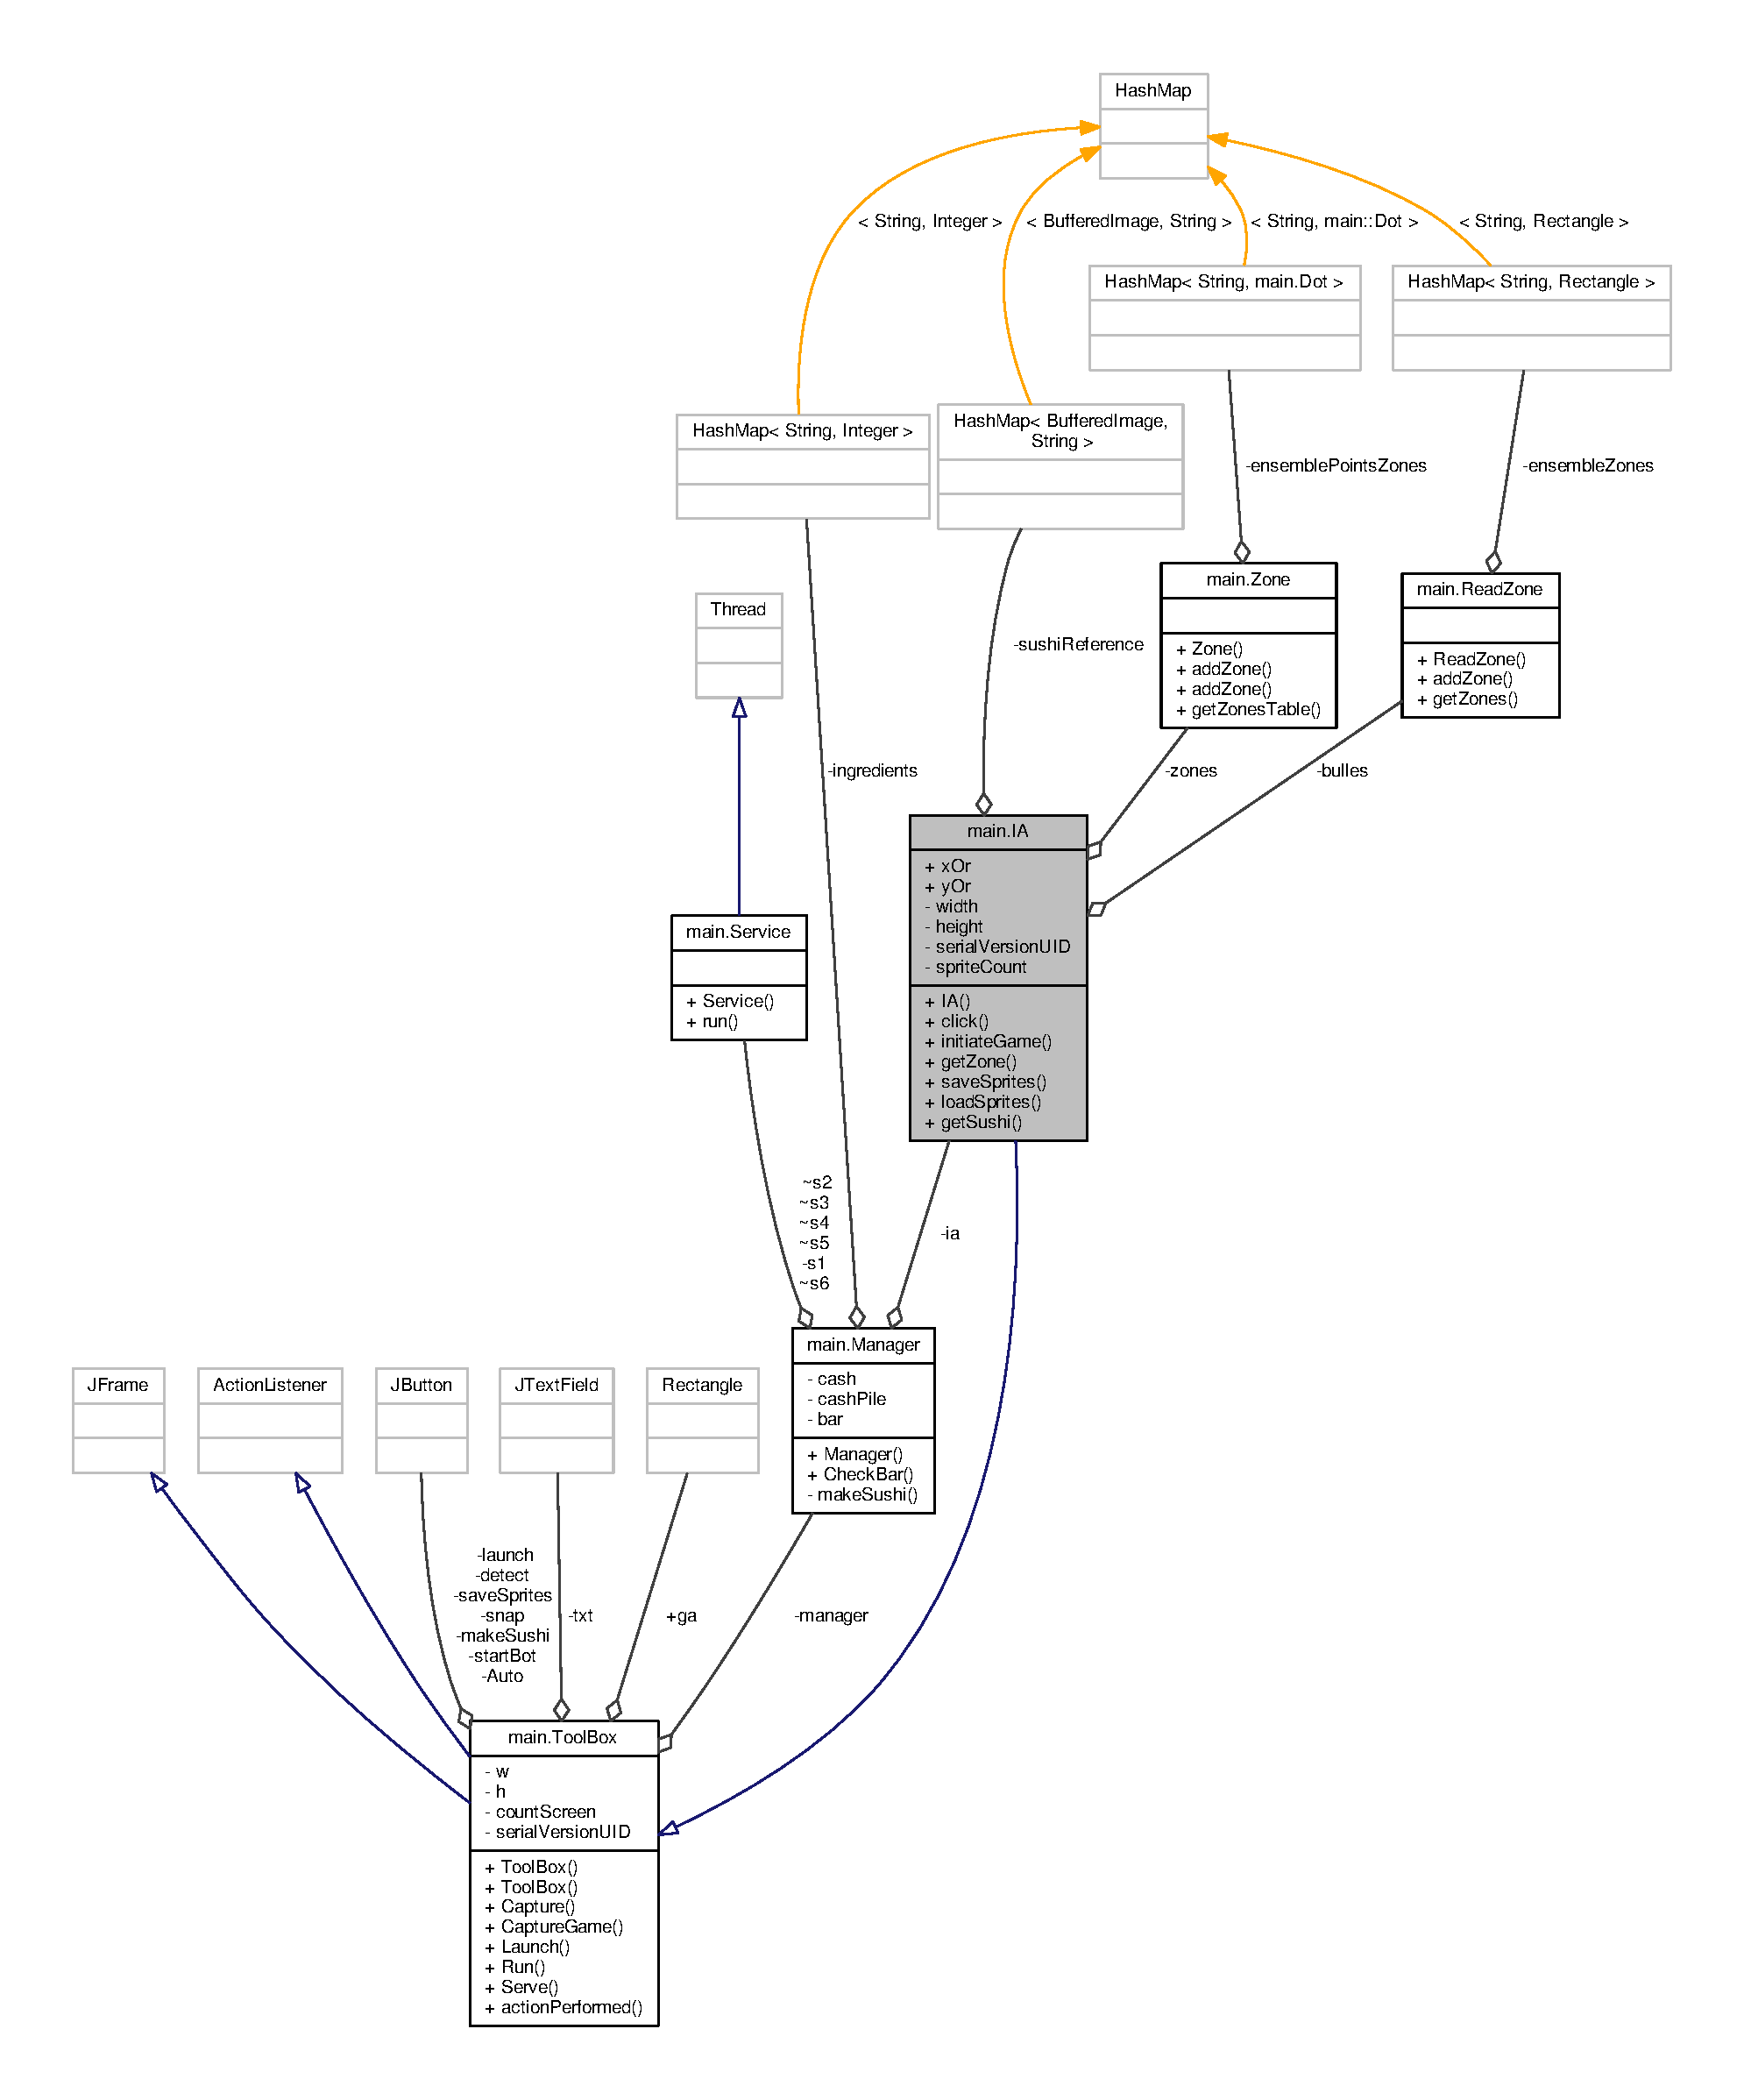
\includegraphics[width=350pt]{classmain_1_1IA__coll__graph}
\end{center}
\end{figure}
\subsubsection*{Fonctions membres publiques}
\begin{DoxyCompactItemize}
\item 
\hyperlink{classmain_1_1IA_abdf61311d6f954412d7090bf475ae14b}{I\+A} (Rectangle rec)  throws A\+W\+T\+Exception 
\item 
void \hyperlink{classmain_1_1IA_a12443a6b5c68cfc5ed228cf95497a289}{click} (String zone)  throws A\+W\+T\+Exception, Interrupted\+Exception 
\item 
void \hyperlink{classmain_1_1IA_ae79d50e08efd41c2bc3e2358813d14a0}{initiate\+Game} ()  throws A\+W\+T\+Exception, Interrupted\+Exception 
\item 
\hyperlink{classmain_1_1Zone}{Zone} \hyperlink{classmain_1_1IA_a38da47f9ebf320139219e88999b5592f}{get\+Zone} ()
\item 
void \hyperlink{classmain_1_1IA_a8402495f47d4e31bf6bfa9cf12d07e82}{save\+Sprites} ()  throws A\+W\+T\+Exception, I\+O\+Exception 
\item 
Array\+List$<$ Buffered\+Image $>$ \hyperlink{classmain_1_1IA_a6dcd1dd3cbfe6b00751a004865062b5a}{load\+Sprites} ()  throws A\+W\+T\+Exception 
\item 
String \hyperlink{classmain_1_1IA_afefd04b6129ccdd869e1f077486a133c}{get\+Sushi} (Buffered\+Image sushi\+To\+Test)
\item 
void \hyperlink{classmain_1_1ToolBox_a33e0e8725b840783eb84374703aebcea}{Capture} ()  throws A\+W\+T\+Exception 
\item 
void \hyperlink{classmain_1_1ToolBox_a01fb48e54f183649df1c9e742b966362}{Capture\+Game} (int tps)  throws A\+W\+T\+Exception 
\item 
void \hyperlink{classmain_1_1ToolBox_a93e4314130826a51bf234791e201bebb}{Launch} ()
\item 
void \hyperlink{classmain_1_1ToolBox_a41a6d959beb73dac4a650719737f5c2c}{Run} ()  throws Interrupted\+Exception, A\+W\+T\+Exception 
\item 
void \hyperlink{classmain_1_1ToolBox_a3ab9626ed8eb24317e4fb8906e215c32}{Serve} ()  throws Interrupted\+Exception 
\item 
void \hyperlink{classmain_1_1ToolBox_a6ff2b68cd96e589959f0b66c45696d07}{action\+Performed} (Action\+Event arg0)
\end{DoxyCompactItemize}
\subsubsection*{Attributs publics statiques}
\begin{DoxyCompactItemize}
\item 
static int \hyperlink{classmain_1_1IA_a6c2449fa683b089211b6ca7a8d062b6f}{x\+Or}
\item 
static int \hyperlink{classmain_1_1IA_a7524049aa635b4a3014aeda29b3735af}{y\+Or}
\item 
static Rectangle \hyperlink{classmain_1_1ToolBox_ab1c5162cc4718a5e4b51430dc6ea7d66}{ga}
\end{DoxyCompactItemize}
\subsubsection*{Attributs privés}
\begin{DoxyCompactItemize}
\item 
int \hyperlink{classmain_1_1IA_a6dea592dda2d0384f60ac162899af281}{width}
\item 
int \hyperlink{classmain_1_1IA_a6bef9c3d6ca423025cd8ce08afe5a6a4}{height}
\item 
\hyperlink{classmain_1_1Zone}{Zone} \hyperlink{classmain_1_1IA_aec81fc287caaa8d7190eb8b5d94e7db5}{zones}
\item 
\hyperlink{classmain_1_1ReadZone}{Read\+Zone} \hyperlink{classmain_1_1IA_ab8bdc0e06f762375f1fcbde6cb4ce9b4}{bulles}
\item 
Hash\+Map$<$ Buffered\+Image, String $>$ \hyperlink{classmain_1_1IA_a0c7ba08450493f98e01cf13812b24bda}{sushi\+Reference}
\end{DoxyCompactItemize}
\subsubsection*{Attributs privés statiques}
\begin{DoxyCompactItemize}
\item 
static final long \hyperlink{classmain_1_1IA_a428eadbb58971a343f8848dea57e5cf3}{serial\+Version\+U\+I\+D} = 5210558056865804594\+L
\item 
static int \hyperlink{classmain_1_1IA_a68c9de6cac561ba82fedfd386c10677e}{sprite\+Count} = 0
\end{DoxyCompactItemize}


\subsubsection{Documentation des constructeurs et destructeur}
\hypertarget{classmain_1_1IA_abdf61311d6f954412d7090bf475ae14b}{}\index{main\+::\+I\+A@{main\+::\+I\+A}!I\+A@{I\+A}}
\index{I\+A@{I\+A}!main\+::\+I\+A@{main\+::\+I\+A}}
\paragraph[{I\+A}]{\setlength{\rightskip}{0pt plus 5cm}main.\+I\+A.\+I\+A (
\begin{DoxyParamCaption}
\item[{Rectangle}]{rec}
\end{DoxyParamCaption}
) throws A\+W\+T\+Exception}\label{classmain_1_1IA_abdf61311d6f954412d7090bf475ae14b}


\subsubsection{Documentation des fonctions membres}
\hypertarget{classmain_1_1ToolBox_a6ff2b68cd96e589959f0b66c45696d07}{}\index{main\+::\+I\+A@{main\+::\+I\+A}!action\+Performed@{action\+Performed}}
\index{action\+Performed@{action\+Performed}!main\+::\+I\+A@{main\+::\+I\+A}}
\paragraph[{action\+Performed}]{\setlength{\rightskip}{0pt plus 5cm}void main.\+Tool\+Box.\+action\+Performed (
\begin{DoxyParamCaption}
\item[{Action\+Event}]{arg0}
\end{DoxyParamCaption}
)\hspace{0.3cm}{\ttfamily [inherited]}}\label{classmain_1_1ToolBox_a6ff2b68cd96e589959f0b66c45696d07}
\hypertarget{classmain_1_1ToolBox_a33e0e8725b840783eb84374703aebcea}{}\index{main\+::\+I\+A@{main\+::\+I\+A}!Capture@{Capture}}
\index{Capture@{Capture}!main\+::\+I\+A@{main\+::\+I\+A}}
\paragraph[{Capture}]{\setlength{\rightskip}{0pt plus 5cm}void main.\+Tool\+Box.\+Capture (
\begin{DoxyParamCaption}
{}
\end{DoxyParamCaption}
) throws A\+W\+T\+Exception\hspace{0.3cm}{\ttfamily [inherited]}}\label{classmain_1_1ToolBox_a33e0e8725b840783eb84374703aebcea}


Référencé par main.\+Tool\+Box.\+action\+Performed().

\hypertarget{classmain_1_1ToolBox_a01fb48e54f183649df1c9e742b966362}{}\index{main\+::\+I\+A@{main\+::\+I\+A}!Capture\+Game@{Capture\+Game}}
\index{Capture\+Game@{Capture\+Game}!main\+::\+I\+A@{main\+::\+I\+A}}
\paragraph[{Capture\+Game}]{\setlength{\rightskip}{0pt plus 5cm}void main.\+Tool\+Box.\+Capture\+Game (
\begin{DoxyParamCaption}
\item[{int}]{tps}
\end{DoxyParamCaption}
) throws A\+W\+T\+Exception\hspace{0.3cm}{\ttfamily [inherited]}}\label{classmain_1_1ToolBox_a01fb48e54f183649df1c9e742b966362}


Référencé par main.\+Tool\+Box.\+action\+Performed().

\hypertarget{classmain_1_1IA_a12443a6b5c68cfc5ed228cf95497a289}{}\index{main\+::\+I\+A@{main\+::\+I\+A}!click@{click}}
\index{click@{click}!main\+::\+I\+A@{main\+::\+I\+A}}
\paragraph[{click}]{\setlength{\rightskip}{0pt plus 5cm}void main.\+I\+A.\+click (
\begin{DoxyParamCaption}
\item[{String}]{zone}
\end{DoxyParamCaption}
) throws A\+W\+T\+Exception, Interrupted\+Exception}\label{classmain_1_1IA_a12443a6b5c68cfc5ed228cf95497a289}


Référencé par main.\+I\+A.\+initiate\+Game(), et main.\+Manager.\+make\+Sushi().

\hypertarget{classmain_1_1IA_afefd04b6129ccdd869e1f077486a133c}{}\index{main\+::\+I\+A@{main\+::\+I\+A}!get\+Sushi@{get\+Sushi}}
\index{get\+Sushi@{get\+Sushi}!main\+::\+I\+A@{main\+::\+I\+A}}
\paragraph[{get\+Sushi}]{\setlength{\rightskip}{0pt plus 5cm}String main.\+I\+A.\+get\+Sushi (
\begin{DoxyParamCaption}
\item[{Buffered\+Image}]{sushi\+To\+Test}
\end{DoxyParamCaption}
)}\label{classmain_1_1IA_afefd04b6129ccdd869e1f077486a133c}


Référencé par main.\+Manager.\+Check\+Bar().

\hypertarget{classmain_1_1IA_a38da47f9ebf320139219e88999b5592f}{}\index{main\+::\+I\+A@{main\+::\+I\+A}!get\+Zone@{get\+Zone}}
\index{get\+Zone@{get\+Zone}!main\+::\+I\+A@{main\+::\+I\+A}}
\paragraph[{get\+Zone}]{\setlength{\rightskip}{0pt plus 5cm}{\bf Zone} main.\+I\+A.\+get\+Zone (
\begin{DoxyParamCaption}
{}
\end{DoxyParamCaption}
)}\label{classmain_1_1IA_a38da47f9ebf320139219e88999b5592f}


Référencé par main.\+I\+A\+Test.\+test().

\hypertarget{classmain_1_1IA_ae79d50e08efd41c2bc3e2358813d14a0}{}\index{main\+::\+I\+A@{main\+::\+I\+A}!initiate\+Game@{initiate\+Game}}
\index{initiate\+Game@{initiate\+Game}!main\+::\+I\+A@{main\+::\+I\+A}}
\paragraph[{initiate\+Game}]{\setlength{\rightskip}{0pt plus 5cm}void main.\+I\+A.\+initiate\+Game (
\begin{DoxyParamCaption}
{}
\end{DoxyParamCaption}
) throws A\+W\+T\+Exception, Interrupted\+Exception}\label{classmain_1_1IA_ae79d50e08efd41c2bc3e2358813d14a0}


Référencé par main.\+Tool\+Box.\+Run().

\hypertarget{classmain_1_1ToolBox_a93e4314130826a51bf234791e201bebb}{}\index{main\+::\+I\+A@{main\+::\+I\+A}!Launch@{Launch}}
\index{Launch@{Launch}!main\+::\+I\+A@{main\+::\+I\+A}}
\paragraph[{Launch}]{\setlength{\rightskip}{0pt plus 5cm}void main.\+Tool\+Box.\+Launch (
\begin{DoxyParamCaption}
{}
\end{DoxyParamCaption}
)\hspace{0.3cm}{\ttfamily [inherited]}}\label{classmain_1_1ToolBox_a93e4314130826a51bf234791e201bebb}


Référencé par main.\+Tool\+Box.\+action\+Performed().

\hypertarget{classmain_1_1IA_a6dcd1dd3cbfe6b00751a004865062b5a}{}\index{main\+::\+I\+A@{main\+::\+I\+A}!load\+Sprites@{load\+Sprites}}
\index{load\+Sprites@{load\+Sprites}!main\+::\+I\+A@{main\+::\+I\+A}}
\paragraph[{load\+Sprites}]{\setlength{\rightskip}{0pt plus 5cm}Array\+List$<$Buffered\+Image$>$ main.\+I\+A.\+load\+Sprites (
\begin{DoxyParamCaption}
{}
\end{DoxyParamCaption}
) throws A\+W\+T\+Exception}\label{classmain_1_1IA_a6dcd1dd3cbfe6b00751a004865062b5a}


Référencé par main.\+Manager.\+Check\+Bar().

\hypertarget{classmain_1_1ToolBox_a41a6d959beb73dac4a650719737f5c2c}{}\index{main\+::\+I\+A@{main\+::\+I\+A}!Run@{Run}}
\index{Run@{Run}!main\+::\+I\+A@{main\+::\+I\+A}}
\paragraph[{Run}]{\setlength{\rightskip}{0pt plus 5cm}void main.\+Tool\+Box.\+Run (
\begin{DoxyParamCaption}
{}
\end{DoxyParamCaption}
) throws Interrupted\+Exception, A\+W\+T\+Exception\hspace{0.3cm}{\ttfamily [inherited]}}\label{classmain_1_1ToolBox_a41a6d959beb73dac4a650719737f5c2c}


Référencé par main.\+Tool\+Box.\+action\+Performed().

\hypertarget{classmain_1_1IA_a8402495f47d4e31bf6bfa9cf12d07e82}{}\index{main\+::\+I\+A@{main\+::\+I\+A}!save\+Sprites@{save\+Sprites}}
\index{save\+Sprites@{save\+Sprites}!main\+::\+I\+A@{main\+::\+I\+A}}
\paragraph[{save\+Sprites}]{\setlength{\rightskip}{0pt plus 5cm}void main.\+I\+A.\+save\+Sprites (
\begin{DoxyParamCaption}
{}
\end{DoxyParamCaption}
) throws A\+W\+T\+Exception, I\+O\+Exception}\label{classmain_1_1IA_a8402495f47d4e31bf6bfa9cf12d07e82}


Référencé par main.\+Tool\+Box.\+action\+Performed().

\hypertarget{classmain_1_1ToolBox_a3ab9626ed8eb24317e4fb8906e215c32}{}\index{main\+::\+I\+A@{main\+::\+I\+A}!Serve@{Serve}}
\index{Serve@{Serve}!main\+::\+I\+A@{main\+::\+I\+A}}
\paragraph[{Serve}]{\setlength{\rightskip}{0pt plus 5cm}void main.\+Tool\+Box.\+Serve (
\begin{DoxyParamCaption}
{}
\end{DoxyParamCaption}
) throws Interrupted\+Exception\hspace{0.3cm}{\ttfamily [inherited]}}\label{classmain_1_1ToolBox_a3ab9626ed8eb24317e4fb8906e215c32}


Référencé par main.\+Tool\+Box.\+action\+Performed().



\subsubsection{Documentation des données membres}
\hypertarget{classmain_1_1IA_ab8bdc0e06f762375f1fcbde6cb4ce9b4}{}\index{main\+::\+I\+A@{main\+::\+I\+A}!bulles@{bulles}}
\index{bulles@{bulles}!main\+::\+I\+A@{main\+::\+I\+A}}
\paragraph[{bulles}]{\setlength{\rightskip}{0pt plus 5cm}{\bf Read\+Zone} main.\+I\+A.\+bulles\hspace{0.3cm}{\ttfamily [private]}}\label{classmain_1_1IA_ab8bdc0e06f762375f1fcbde6cb4ce9b4}
\hypertarget{classmain_1_1ToolBox_ab1c5162cc4718a5e4b51430dc6ea7d66}{}\index{main\+::\+I\+A@{main\+::\+I\+A}!ga@{ga}}
\index{ga@{ga}!main\+::\+I\+A@{main\+::\+I\+A}}
\paragraph[{ga}]{\setlength{\rightskip}{0pt plus 5cm}Rectangle main.\+Tool\+Box.\+ga\hspace{0.3cm}{\ttfamily [static]}, {\ttfamily [inherited]}}\label{classmain_1_1ToolBox_ab1c5162cc4718a5e4b51430dc6ea7d66}


Référencé par main.\+Manager.\+Manager().

\hypertarget{classmain_1_1IA_a6bef9c3d6ca423025cd8ce08afe5a6a4}{}\index{main\+::\+I\+A@{main\+::\+I\+A}!height@{height}}
\index{height@{height}!main\+::\+I\+A@{main\+::\+I\+A}}
\paragraph[{height}]{\setlength{\rightskip}{0pt plus 5cm}int main.\+I\+A.\+height\hspace{0.3cm}{\ttfamily [private]}}\label{classmain_1_1IA_a6bef9c3d6ca423025cd8ce08afe5a6a4}
\hypertarget{classmain_1_1IA_a428eadbb58971a343f8848dea57e5cf3}{}\index{main\+::\+I\+A@{main\+::\+I\+A}!serial\+Version\+U\+I\+D@{serial\+Version\+U\+I\+D}}
\index{serial\+Version\+U\+I\+D@{serial\+Version\+U\+I\+D}!main\+::\+I\+A@{main\+::\+I\+A}}
\paragraph[{serial\+Version\+U\+I\+D}]{\setlength{\rightskip}{0pt plus 5cm}final long main.\+I\+A.\+serial\+Version\+U\+I\+D = 5210558056865804594\+L\hspace{0.3cm}{\ttfamily [static]}, {\ttfamily [private]}}\label{classmain_1_1IA_a428eadbb58971a343f8848dea57e5cf3}
\hypertarget{classmain_1_1IA_a68c9de6cac561ba82fedfd386c10677e}{}\index{main\+::\+I\+A@{main\+::\+I\+A}!sprite\+Count@{sprite\+Count}}
\index{sprite\+Count@{sprite\+Count}!main\+::\+I\+A@{main\+::\+I\+A}}
\paragraph[{sprite\+Count}]{\setlength{\rightskip}{0pt plus 5cm}int main.\+I\+A.\+sprite\+Count = 0\hspace{0.3cm}{\ttfamily [static]}, {\ttfamily [private]}}\label{classmain_1_1IA_a68c9de6cac561ba82fedfd386c10677e}
\hypertarget{classmain_1_1IA_a0c7ba08450493f98e01cf13812b24bda}{}\index{main\+::\+I\+A@{main\+::\+I\+A}!sushi\+Reference@{sushi\+Reference}}
\index{sushi\+Reference@{sushi\+Reference}!main\+::\+I\+A@{main\+::\+I\+A}}
\paragraph[{sushi\+Reference}]{\setlength{\rightskip}{0pt plus 5cm}Hash\+Map$<$Buffered\+Image, String$>$ main.\+I\+A.\+sushi\+Reference\hspace{0.3cm}{\ttfamily [private]}}\label{classmain_1_1IA_a0c7ba08450493f98e01cf13812b24bda}
\hypertarget{classmain_1_1IA_a6dea592dda2d0384f60ac162899af281}{}\index{main\+::\+I\+A@{main\+::\+I\+A}!width@{width}}
\index{width@{width}!main\+::\+I\+A@{main\+::\+I\+A}}
\paragraph[{width}]{\setlength{\rightskip}{0pt plus 5cm}int main.\+I\+A.\+width\hspace{0.3cm}{\ttfamily [private]}}\label{classmain_1_1IA_a6dea592dda2d0384f60ac162899af281}
\hypertarget{classmain_1_1IA_a6c2449fa683b089211b6ca7a8d062b6f}{}\index{main\+::\+I\+A@{main\+::\+I\+A}!x\+Or@{x\+Or}}
\index{x\+Or@{x\+Or}!main\+::\+I\+A@{main\+::\+I\+A}}
\paragraph[{x\+Or}]{\setlength{\rightskip}{0pt plus 5cm}int main.\+I\+A.\+x\+Or\hspace{0.3cm}{\ttfamily [static]}}\label{classmain_1_1IA_a6c2449fa683b089211b6ca7a8d062b6f}


Référencé par main.\+Dot.\+translate().

\hypertarget{classmain_1_1IA_a7524049aa635b4a3014aeda29b3735af}{}\index{main\+::\+I\+A@{main\+::\+I\+A}!y\+Or@{y\+Or}}
\index{y\+Or@{y\+Or}!main\+::\+I\+A@{main\+::\+I\+A}}
\paragraph[{y\+Or}]{\setlength{\rightskip}{0pt plus 5cm}int main.\+I\+A.\+y\+Or\hspace{0.3cm}{\ttfamily [static]}}\label{classmain_1_1IA_a7524049aa635b4a3014aeda29b3735af}


Référencé par main.\+Dot.\+translate().

\hypertarget{classmain_1_1IA_aec81fc287caaa8d7190eb8b5d94e7db5}{}\index{main\+::\+I\+A@{main\+::\+I\+A}!zones@{zones}}
\index{zones@{zones}!main\+::\+I\+A@{main\+::\+I\+A}}
\paragraph[{zones}]{\setlength{\rightskip}{0pt plus 5cm}{\bf Zone} main.\+I\+A.\+zones\hspace{0.3cm}{\ttfamily [private]}}\label{classmain_1_1IA_aec81fc287caaa8d7190eb8b5d94e7db5}


Référencé par main.\+I\+A.\+get\+Zone().



La documentation de cette classe a été générée à partir du fichier suivant \+:\begin{DoxyCompactItemize}
\item 
\hyperlink{main_2IA_8java}{main/\+I\+A.\+java}\end{DoxyCompactItemize}

\hypertarget{classSushis_1_1src_1_1IA}{}\subsection{Référence de la classe Sushis.\+src.\+I\+A}
\label{classSushis_1_1src_1_1IA}\index{Sushis.\+src.\+I\+A@{Sushis.\+src.\+I\+A}}


Graphe d\textquotesingle{}héritage de Sushis.\+src.\+I\+A\+:\nopagebreak
\begin{figure}[H]
\begin{center}
\leavevmode
\includegraphics[height=550pt]{classSushis_1_1src_1_1IA__inherit__graph}
\end{center}
\end{figure}


Graphe de collaboration de Sushis.\+src.\+I\+A\+:\nopagebreak
\begin{figure}[H]
\begin{center}
\leavevmode
\includegraphics[width=350pt]{classSushis_1_1src_1_1IA__coll__graph}
\end{center}
\end{figure}
\subsubsection*{Fonctions membres publiques}
\begin{DoxyCompactItemize}
\item 
\hyperlink{classSushis_1_1src_1_1IA_ae09b1ae66dfec966050bde22afebf409}{I\+A} (Rectangle rec)  throws A\+W\+T\+Exception 
\item 
void \hyperlink{classSushis_1_1src_1_1IA_a6cfc37df4fd2a02cf6b75abb3f3bdfc6}{click} (String zone)  throws A\+W\+T\+Exception, Interrupted\+Exception 
\item 
void \hyperlink{classSushis_1_1src_1_1IA_ad4ad87f8107d1c7f5cf520ac1322e1f4}{initiate\+Game} ()  throws A\+W\+T\+Exception, Interrupted\+Exception 
\item 
\hyperlink{classSushis_1_1src_1_1Zone}{Zone} \hyperlink{classSushis_1_1src_1_1IA_a93671a60ef14f7bc5ab5ad1cad0066a9}{get\+Zone} ()
\item 
void \hyperlink{classSushis_1_1src_1_1IA_ab80d7759fd410f391118e5fea2fb4c30}{save\+Sprites} ()  throws A\+W\+T\+Exception, I\+O\+Exception 
\item 
Array\+List$<$ Buffered\+Image $>$ \hyperlink{classSushis_1_1src_1_1IA_a17ae4bc6c3a8949a667a893a24413d19}{load\+Sprites} ()  throws A\+W\+T\+Exception 
\item 
String \hyperlink{classSushis_1_1src_1_1IA_aeeb6af348f605d72fa13038d47fe8bbb}{get\+Sushi} (Buffered\+Image sushi\+To\+Test)
\item 
void \hyperlink{classSushis_1_1src_1_1ToolBox_ade4282ccb35c18dd7cd473c680145b86}{Capture} ()  throws A\+W\+T\+Exception 
\item 
void \hyperlink{classSushis_1_1src_1_1ToolBox_a85ac3d5ce3aa8a7a3691f6dbbc000aed}{Capture\+Game} (int tps)  throws A\+W\+T\+Exception 
\item 
void \hyperlink{classSushis_1_1src_1_1ToolBox_afac5ed37e5905a6409a375e5ad2000b2}{Launch} ()
\item 
void \hyperlink{classSushis_1_1src_1_1ToolBox_a2542efab6381677391dfe6407c0db0f7}{Run} ()  throws Interrupted\+Exception, A\+W\+T\+Exception 
\item 
void \hyperlink{classSushis_1_1src_1_1ToolBox_adad53308af901ed75c8ddd16e7069e6d}{Serve} ()  throws Interrupted\+Exception 
\item 
void \hyperlink{classSushis_1_1src_1_1ToolBox_a5c3c1e9751ac4cd49965024ae0485e56}{action\+Performed} (Action\+Event arg0)
\end{DoxyCompactItemize}
\subsubsection*{Attributs publics statiques}
\begin{DoxyCompactItemize}
\item 
static int \hyperlink{classSushis_1_1src_1_1IA_aaa01e3156a3a39dd19701e89d4518c2b}{x\+Or}
\item 
static int \hyperlink{classSushis_1_1src_1_1IA_aa970ffebf19547e72c59f109c428ef14}{y\+Or}
\item 
static Rectangle \hyperlink{classSushis_1_1src_1_1ToolBox_a614f944df0493f7be8fcdad36d3265b7}{ga}
\end{DoxyCompactItemize}
\subsubsection*{Attributs privés}
\begin{DoxyCompactItemize}
\item 
int \hyperlink{classSushis_1_1src_1_1IA_ae72069abf3035484ac8c0acd9dadbb4a}{width}
\item 
int \hyperlink{classSushis_1_1src_1_1IA_a0175491438b89afa128cdba5619debbe}{height}
\item 
\hyperlink{classSushis_1_1src_1_1Zone}{Zone} \hyperlink{classSushis_1_1src_1_1IA_a019c981a7f6d249d7b7c54fb08edaa67}{zones}
\item 
\hyperlink{classSushis_1_1src_1_1ReadZone}{Read\+Zone} \hyperlink{classSushis_1_1src_1_1IA_a18b0a2294f283c7922470cea926a198b}{bulles}
\item 
Hash\+Map$<$ Buffered\+Image, String $>$ \hyperlink{classSushis_1_1src_1_1IA_a0e930e667457530a6adbf23aaca3de54}{sushi\+Reference}
\end{DoxyCompactItemize}
\subsubsection*{Attributs privés statiques}
\begin{DoxyCompactItemize}
\item 
static final long \hyperlink{classSushis_1_1src_1_1IA_a0b3532db3833b821234054562c23eff1}{serial\+Version\+U\+I\+D} = 5210558056865804594\+L
\item 
static int \hyperlink{classSushis_1_1src_1_1IA_aa7ae1d8827fe4f4d3af0a5d9cb4f8b62}{sprite\+Count} = 0
\end{DoxyCompactItemize}


\subsubsection{Documentation des constructeurs et destructeur}
\hypertarget{classSushis_1_1src_1_1IA_ae09b1ae66dfec966050bde22afebf409}{}\index{Sushis\+::src\+::\+I\+A@{Sushis\+::src\+::\+I\+A}!I\+A@{I\+A}}
\index{I\+A@{I\+A}!Sushis\+::src\+::\+I\+A@{Sushis\+::src\+::\+I\+A}}
\paragraph[{I\+A}]{\setlength{\rightskip}{0pt plus 5cm}Sushis.\+src.\+I\+A.\+I\+A (
\begin{DoxyParamCaption}
\item[{Rectangle}]{rec}
\end{DoxyParamCaption}
) throws A\+W\+T\+Exception}\label{classSushis_1_1src_1_1IA_ae09b1ae66dfec966050bde22afebf409}


\subsubsection{Documentation des fonctions membres}
\hypertarget{classSushis_1_1src_1_1ToolBox_a5c3c1e9751ac4cd49965024ae0485e56}{}\index{Sushis\+::src\+::\+I\+A@{Sushis\+::src\+::\+I\+A}!action\+Performed@{action\+Performed}}
\index{action\+Performed@{action\+Performed}!Sushis\+::src\+::\+I\+A@{Sushis\+::src\+::\+I\+A}}
\paragraph[{action\+Performed}]{\setlength{\rightskip}{0pt plus 5cm}void Sushis.\+src.\+Tool\+Box.\+action\+Performed (
\begin{DoxyParamCaption}
\item[{Action\+Event}]{arg0}
\end{DoxyParamCaption}
)\hspace{0.3cm}{\ttfamily [inherited]}}\label{classSushis_1_1src_1_1ToolBox_a5c3c1e9751ac4cd49965024ae0485e56}
\hypertarget{classSushis_1_1src_1_1ToolBox_ade4282ccb35c18dd7cd473c680145b86}{}\index{Sushis\+::src\+::\+I\+A@{Sushis\+::src\+::\+I\+A}!Capture@{Capture}}
\index{Capture@{Capture}!Sushis\+::src\+::\+I\+A@{Sushis\+::src\+::\+I\+A}}
\paragraph[{Capture}]{\setlength{\rightskip}{0pt plus 5cm}void Sushis.\+src.\+Tool\+Box.\+Capture (
\begin{DoxyParamCaption}
{}
\end{DoxyParamCaption}
) throws A\+W\+T\+Exception\hspace{0.3cm}{\ttfamily [inherited]}}\label{classSushis_1_1src_1_1ToolBox_ade4282ccb35c18dd7cd473c680145b86}


Référencé par Sushis.\+src.\+Tool\+Box.\+action\+Performed().

\hypertarget{classSushis_1_1src_1_1ToolBox_a85ac3d5ce3aa8a7a3691f6dbbc000aed}{}\index{Sushis\+::src\+::\+I\+A@{Sushis\+::src\+::\+I\+A}!Capture\+Game@{Capture\+Game}}
\index{Capture\+Game@{Capture\+Game}!Sushis\+::src\+::\+I\+A@{Sushis\+::src\+::\+I\+A}}
\paragraph[{Capture\+Game}]{\setlength{\rightskip}{0pt plus 5cm}void Sushis.\+src.\+Tool\+Box.\+Capture\+Game (
\begin{DoxyParamCaption}
\item[{int}]{tps}
\end{DoxyParamCaption}
) throws A\+W\+T\+Exception\hspace{0.3cm}{\ttfamily [inherited]}}\label{classSushis_1_1src_1_1ToolBox_a85ac3d5ce3aa8a7a3691f6dbbc000aed}


Référencé par Sushis.\+src.\+Tool\+Box.\+action\+Performed().

\hypertarget{classSushis_1_1src_1_1IA_a6cfc37df4fd2a02cf6b75abb3f3bdfc6}{}\index{Sushis\+::src\+::\+I\+A@{Sushis\+::src\+::\+I\+A}!click@{click}}
\index{click@{click}!Sushis\+::src\+::\+I\+A@{Sushis\+::src\+::\+I\+A}}
\paragraph[{click}]{\setlength{\rightskip}{0pt plus 5cm}void Sushis.\+src.\+I\+A.\+click (
\begin{DoxyParamCaption}
\item[{String}]{zone}
\end{DoxyParamCaption}
) throws A\+W\+T\+Exception, Interrupted\+Exception}\label{classSushis_1_1src_1_1IA_a6cfc37df4fd2a02cf6b75abb3f3bdfc6}


Référencé par Sushis.\+src.\+I\+A.\+initiate\+Game(), et Sushis.\+src.\+Manager.\+make\+Sushi().

\hypertarget{classSushis_1_1src_1_1IA_aeeb6af348f605d72fa13038d47fe8bbb}{}\index{Sushis\+::src\+::\+I\+A@{Sushis\+::src\+::\+I\+A}!get\+Sushi@{get\+Sushi}}
\index{get\+Sushi@{get\+Sushi}!Sushis\+::src\+::\+I\+A@{Sushis\+::src\+::\+I\+A}}
\paragraph[{get\+Sushi}]{\setlength{\rightskip}{0pt plus 5cm}String Sushis.\+src.\+I\+A.\+get\+Sushi (
\begin{DoxyParamCaption}
\item[{Buffered\+Image}]{sushi\+To\+Test}
\end{DoxyParamCaption}
)}\label{classSushis_1_1src_1_1IA_aeeb6af348f605d72fa13038d47fe8bbb}


Référencé par Sushis.\+src.\+Manager.\+Check\+Bar().

\hypertarget{classSushis_1_1src_1_1IA_a93671a60ef14f7bc5ab5ad1cad0066a9}{}\index{Sushis\+::src\+::\+I\+A@{Sushis\+::src\+::\+I\+A}!get\+Zone@{get\+Zone}}
\index{get\+Zone@{get\+Zone}!Sushis\+::src\+::\+I\+A@{Sushis\+::src\+::\+I\+A}}
\paragraph[{get\+Zone}]{\setlength{\rightskip}{0pt plus 5cm}{\bf Zone} Sushis.\+src.\+I\+A.\+get\+Zone (
\begin{DoxyParamCaption}
{}
\end{DoxyParamCaption}
)}\label{classSushis_1_1src_1_1IA_a93671a60ef14f7bc5ab5ad1cad0066a9}
\hypertarget{classSushis_1_1src_1_1IA_ad4ad87f8107d1c7f5cf520ac1322e1f4}{}\index{Sushis\+::src\+::\+I\+A@{Sushis\+::src\+::\+I\+A}!initiate\+Game@{initiate\+Game}}
\index{initiate\+Game@{initiate\+Game}!Sushis\+::src\+::\+I\+A@{Sushis\+::src\+::\+I\+A}}
\paragraph[{initiate\+Game}]{\setlength{\rightskip}{0pt plus 5cm}void Sushis.\+src.\+I\+A.\+initiate\+Game (
\begin{DoxyParamCaption}
{}
\end{DoxyParamCaption}
) throws A\+W\+T\+Exception, Interrupted\+Exception}\label{classSushis_1_1src_1_1IA_ad4ad87f8107d1c7f5cf520ac1322e1f4}


Référencé par Sushis.\+src.\+Tool\+Box.\+Run().

\hypertarget{classSushis_1_1src_1_1ToolBox_afac5ed37e5905a6409a375e5ad2000b2}{}\index{Sushis\+::src\+::\+I\+A@{Sushis\+::src\+::\+I\+A}!Launch@{Launch}}
\index{Launch@{Launch}!Sushis\+::src\+::\+I\+A@{Sushis\+::src\+::\+I\+A}}
\paragraph[{Launch}]{\setlength{\rightskip}{0pt plus 5cm}void Sushis.\+src.\+Tool\+Box.\+Launch (
\begin{DoxyParamCaption}
{}
\end{DoxyParamCaption}
)\hspace{0.3cm}{\ttfamily [inherited]}}\label{classSushis_1_1src_1_1ToolBox_afac5ed37e5905a6409a375e5ad2000b2}


Référencé par Sushis.\+src.\+Tool\+Box.\+action\+Performed().

\hypertarget{classSushis_1_1src_1_1IA_a17ae4bc6c3a8949a667a893a24413d19}{}\index{Sushis\+::src\+::\+I\+A@{Sushis\+::src\+::\+I\+A}!load\+Sprites@{load\+Sprites}}
\index{load\+Sprites@{load\+Sprites}!Sushis\+::src\+::\+I\+A@{Sushis\+::src\+::\+I\+A}}
\paragraph[{load\+Sprites}]{\setlength{\rightskip}{0pt plus 5cm}Array\+List$<$Buffered\+Image$>$ Sushis.\+src.\+I\+A.\+load\+Sprites (
\begin{DoxyParamCaption}
{}
\end{DoxyParamCaption}
) throws A\+W\+T\+Exception}\label{classSushis_1_1src_1_1IA_a17ae4bc6c3a8949a667a893a24413d19}


Référencé par Sushis.\+src.\+Manager.\+Check\+Bar().

\hypertarget{classSushis_1_1src_1_1ToolBox_a2542efab6381677391dfe6407c0db0f7}{}\index{Sushis\+::src\+::\+I\+A@{Sushis\+::src\+::\+I\+A}!Run@{Run}}
\index{Run@{Run}!Sushis\+::src\+::\+I\+A@{Sushis\+::src\+::\+I\+A}}
\paragraph[{Run}]{\setlength{\rightskip}{0pt plus 5cm}void Sushis.\+src.\+Tool\+Box.\+Run (
\begin{DoxyParamCaption}
{}
\end{DoxyParamCaption}
) throws Interrupted\+Exception, A\+W\+T\+Exception\hspace{0.3cm}{\ttfamily [inherited]}}\label{classSushis_1_1src_1_1ToolBox_a2542efab6381677391dfe6407c0db0f7}


Référencé par Sushis.\+src.\+Tool\+Box.\+action\+Performed().

\hypertarget{classSushis_1_1src_1_1IA_ab80d7759fd410f391118e5fea2fb4c30}{}\index{Sushis\+::src\+::\+I\+A@{Sushis\+::src\+::\+I\+A}!save\+Sprites@{save\+Sprites}}
\index{save\+Sprites@{save\+Sprites}!Sushis\+::src\+::\+I\+A@{Sushis\+::src\+::\+I\+A}}
\paragraph[{save\+Sprites}]{\setlength{\rightskip}{0pt plus 5cm}void Sushis.\+src.\+I\+A.\+save\+Sprites (
\begin{DoxyParamCaption}
{}
\end{DoxyParamCaption}
) throws A\+W\+T\+Exception, I\+O\+Exception}\label{classSushis_1_1src_1_1IA_ab80d7759fd410f391118e5fea2fb4c30}


Référencé par Sushis.\+src.\+Tool\+Box.\+action\+Performed().

\hypertarget{classSushis_1_1src_1_1ToolBox_adad53308af901ed75c8ddd16e7069e6d}{}\index{Sushis\+::src\+::\+I\+A@{Sushis\+::src\+::\+I\+A}!Serve@{Serve}}
\index{Serve@{Serve}!Sushis\+::src\+::\+I\+A@{Sushis\+::src\+::\+I\+A}}
\paragraph[{Serve}]{\setlength{\rightskip}{0pt plus 5cm}void Sushis.\+src.\+Tool\+Box.\+Serve (
\begin{DoxyParamCaption}
{}
\end{DoxyParamCaption}
) throws Interrupted\+Exception\hspace{0.3cm}{\ttfamily [inherited]}}\label{classSushis_1_1src_1_1ToolBox_adad53308af901ed75c8ddd16e7069e6d}


Référencé par Sushis.\+src.\+Tool\+Box.\+action\+Performed().



\subsubsection{Documentation des données membres}
\hypertarget{classSushis_1_1src_1_1IA_a18b0a2294f283c7922470cea926a198b}{}\index{Sushis\+::src\+::\+I\+A@{Sushis\+::src\+::\+I\+A}!bulles@{bulles}}
\index{bulles@{bulles}!Sushis\+::src\+::\+I\+A@{Sushis\+::src\+::\+I\+A}}
\paragraph[{bulles}]{\setlength{\rightskip}{0pt plus 5cm}{\bf Read\+Zone} Sushis.\+src.\+I\+A.\+bulles\hspace{0.3cm}{\ttfamily [private]}}\label{classSushis_1_1src_1_1IA_a18b0a2294f283c7922470cea926a198b}
\hypertarget{classSushis_1_1src_1_1ToolBox_a614f944df0493f7be8fcdad36d3265b7}{}\index{Sushis\+::src\+::\+I\+A@{Sushis\+::src\+::\+I\+A}!ga@{ga}}
\index{ga@{ga}!Sushis\+::src\+::\+I\+A@{Sushis\+::src\+::\+I\+A}}
\paragraph[{ga}]{\setlength{\rightskip}{0pt plus 5cm}Rectangle Sushis.\+src.\+Tool\+Box.\+ga\hspace{0.3cm}{\ttfamily [static]}, {\ttfamily [inherited]}}\label{classSushis_1_1src_1_1ToolBox_a614f944df0493f7be8fcdad36d3265b7}


Référencé par Sushis.\+src.\+Manager.\+Manager().

\hypertarget{classSushis_1_1src_1_1IA_a0175491438b89afa128cdba5619debbe}{}\index{Sushis\+::src\+::\+I\+A@{Sushis\+::src\+::\+I\+A}!height@{height}}
\index{height@{height}!Sushis\+::src\+::\+I\+A@{Sushis\+::src\+::\+I\+A}}
\paragraph[{height}]{\setlength{\rightskip}{0pt plus 5cm}int Sushis.\+src.\+I\+A.\+height\hspace{0.3cm}{\ttfamily [private]}}\label{classSushis_1_1src_1_1IA_a0175491438b89afa128cdba5619debbe}
\hypertarget{classSushis_1_1src_1_1IA_a0b3532db3833b821234054562c23eff1}{}\index{Sushis\+::src\+::\+I\+A@{Sushis\+::src\+::\+I\+A}!serial\+Version\+U\+I\+D@{serial\+Version\+U\+I\+D}}
\index{serial\+Version\+U\+I\+D@{serial\+Version\+U\+I\+D}!Sushis\+::src\+::\+I\+A@{Sushis\+::src\+::\+I\+A}}
\paragraph[{serial\+Version\+U\+I\+D}]{\setlength{\rightskip}{0pt plus 5cm}final long Sushis.\+src.\+I\+A.\+serial\+Version\+U\+I\+D = 5210558056865804594\+L\hspace{0.3cm}{\ttfamily [static]}, {\ttfamily [private]}}\label{classSushis_1_1src_1_1IA_a0b3532db3833b821234054562c23eff1}
\hypertarget{classSushis_1_1src_1_1IA_aa7ae1d8827fe4f4d3af0a5d9cb4f8b62}{}\index{Sushis\+::src\+::\+I\+A@{Sushis\+::src\+::\+I\+A}!sprite\+Count@{sprite\+Count}}
\index{sprite\+Count@{sprite\+Count}!Sushis\+::src\+::\+I\+A@{Sushis\+::src\+::\+I\+A}}
\paragraph[{sprite\+Count}]{\setlength{\rightskip}{0pt plus 5cm}int Sushis.\+src.\+I\+A.\+sprite\+Count = 0\hspace{0.3cm}{\ttfamily [static]}, {\ttfamily [private]}}\label{classSushis_1_1src_1_1IA_aa7ae1d8827fe4f4d3af0a5d9cb4f8b62}
\hypertarget{classSushis_1_1src_1_1IA_a0e930e667457530a6adbf23aaca3de54}{}\index{Sushis\+::src\+::\+I\+A@{Sushis\+::src\+::\+I\+A}!sushi\+Reference@{sushi\+Reference}}
\index{sushi\+Reference@{sushi\+Reference}!Sushis\+::src\+::\+I\+A@{Sushis\+::src\+::\+I\+A}}
\paragraph[{sushi\+Reference}]{\setlength{\rightskip}{0pt plus 5cm}Hash\+Map$<$Buffered\+Image, String$>$ Sushis.\+src.\+I\+A.\+sushi\+Reference\hspace{0.3cm}{\ttfamily [private]}}\label{classSushis_1_1src_1_1IA_a0e930e667457530a6adbf23aaca3de54}
\hypertarget{classSushis_1_1src_1_1IA_ae72069abf3035484ac8c0acd9dadbb4a}{}\index{Sushis\+::src\+::\+I\+A@{Sushis\+::src\+::\+I\+A}!width@{width}}
\index{width@{width}!Sushis\+::src\+::\+I\+A@{Sushis\+::src\+::\+I\+A}}
\paragraph[{width}]{\setlength{\rightskip}{0pt plus 5cm}int Sushis.\+src.\+I\+A.\+width\hspace{0.3cm}{\ttfamily [private]}}\label{classSushis_1_1src_1_1IA_ae72069abf3035484ac8c0acd9dadbb4a}
\hypertarget{classSushis_1_1src_1_1IA_aaa01e3156a3a39dd19701e89d4518c2b}{}\index{Sushis\+::src\+::\+I\+A@{Sushis\+::src\+::\+I\+A}!x\+Or@{x\+Or}}
\index{x\+Or@{x\+Or}!Sushis\+::src\+::\+I\+A@{Sushis\+::src\+::\+I\+A}}
\paragraph[{x\+Or}]{\setlength{\rightskip}{0pt plus 5cm}int Sushis.\+src.\+I\+A.\+x\+Or\hspace{0.3cm}{\ttfamily [static]}}\label{classSushis_1_1src_1_1IA_aaa01e3156a3a39dd19701e89d4518c2b}
\hypertarget{classSushis_1_1src_1_1IA_aa970ffebf19547e72c59f109c428ef14}{}\index{Sushis\+::src\+::\+I\+A@{Sushis\+::src\+::\+I\+A}!y\+Or@{y\+Or}}
\index{y\+Or@{y\+Or}!Sushis\+::src\+::\+I\+A@{Sushis\+::src\+::\+I\+A}}
\paragraph[{y\+Or}]{\setlength{\rightskip}{0pt plus 5cm}int Sushis.\+src.\+I\+A.\+y\+Or\hspace{0.3cm}{\ttfamily [static]}}\label{classSushis_1_1src_1_1IA_aa970ffebf19547e72c59f109c428ef14}
\hypertarget{classSushis_1_1src_1_1IA_a019c981a7f6d249d7b7c54fb08edaa67}{}\index{Sushis\+::src\+::\+I\+A@{Sushis\+::src\+::\+I\+A}!zones@{zones}}
\index{zones@{zones}!Sushis\+::src\+::\+I\+A@{Sushis\+::src\+::\+I\+A}}
\paragraph[{zones}]{\setlength{\rightskip}{0pt plus 5cm}{\bf Zone} Sushis.\+src.\+I\+A.\+zones\hspace{0.3cm}{\ttfamily [private]}}\label{classSushis_1_1src_1_1IA_a019c981a7f6d249d7b7c54fb08edaa67}


Référencé par Sushis.\+src.\+I\+A.\+get\+Zone().



La documentation de cette classe a été générée à partir du fichier suivant \+:\begin{DoxyCompactItemize}
\item 
\hyperlink{projet_2Sushis_2src_2IA_8java}{projet/\+Sushis/src/\+I\+A.\+java}\end{DoxyCompactItemize}

\hypertarget{classSuchi_1_1Ia}{}\subsection{Référence de la classe Suchi.\+Ia}
\label{classSuchi_1_1Ia}\index{Suchi.\+Ia@{Suchi.\+Ia}}


Graphe de collaboration de Suchi.\+Ia\+:\nopagebreak
\begin{figure}[H]
\begin{center}
\leavevmode
\includegraphics[width=350pt]{classSuchi_1_1Ia__coll__graph}
\end{center}
\end{figure}
\subsubsection*{Fonctions membres publiques}
\begin{DoxyCompactItemize}
\item 
\hyperlink{classSuchi_1_1Ia_a9c574fcd317f6c966660ab8d574c2512}{Ia} ()  throws A\+W\+T\+Exception 
\item 
Buffered\+Image\mbox{[}$\,$\mbox{]} \hyperlink{classSuchi_1_1Ia_a2559a253edf5da792054789e987916e2}{load\+Commandes} ()  throws A\+W\+T\+Exception 
\item 
void \hyperlink{classSuchi_1_1Ia_a4ed4989c340ab5093c939a3d2c57237b}{clear\+Table} ()  throws Exception 
\item 
void \hyperlink{classSuchi_1_1Ia_a547537305068065717526b2c851bcc95}{save\+Sprites} ()  throws A\+W\+T\+Exception, I\+O\+Exception 
\item 
void \hyperlink{classSuchi_1_1Ia_ab3a8439dc96e3510a8608653bb905f31}{fill\+Grey\+Table} (String name, \hyperlink{classSuchi_1_1Dot}{Dot} haut\+Gauche, double \hyperlink{classSuchi_1_1Ia_a12da02ac75078cffa5ab4f3562a6ee98}{width}, double \hyperlink{classSuchi_1_1Ia_af7ce6cad6d21a47c9c31559657a9f000}{height})
\item 
void \hyperlink{classSuchi_1_1Ia_aac06aa97debea740baf03ebaf7d55f5e}{init\+Grey\+Reference} ()  throws Exception 
\item 
void \hyperlink{classSuchi_1_1Ia_a587016dd202f4b315f396f6b2da3660b}{fill\+Commandes} (String name, \hyperlink{classSuchi_1_1Dot}{Dot} haut\+Gauche, double \hyperlink{classSuchi_1_1Ia_a12da02ac75078cffa5ab4f3562a6ee98}{width}, double \hyperlink{classSuchi_1_1Ia_af7ce6cad6d21a47c9c31559657a9f000}{height})
\item 
\hyperlink{classSuchi_1_1Dot}{Dot} \hyperlink{classSuchi_1_1Ia_a3f0bcdc109bbd488785f8c281aa251b7}{get\+Zone} (String s)
\item 
void \hyperlink{classSuchi_1_1Ia_a966d4dfabbbe88f5b797794f1b6b3c4e}{click\+Zone} (String s)  throws Exception 
\item 
void \hyperlink{classSuchi_1_1Ia_a0e55355d2f0ba08d1f7cbb4e30ed26af}{reset\+Ingredients} ()
\item 
void \hyperlink{classSuchi_1_1Ia_a2f66e140aa14567ba4aa99afc4a637b8}{use\+Ingredient} (String s)  throws Exception 
\item 
void \hyperlink{classSuchi_1_1Ia_a58609a5b202ad50445278555a445f2ef}{check\+Ingredients} ()  throws Exception 
\item 
void \hyperlink{classSuchi_1_1Ia_abaca0c75310f60e7d7d172b5c4b0606b}{buy\+Ingredient} (String s)  throws Exception 
\end{DoxyCompactItemize}
\subsubsection*{Attributs de paquetage}
\begin{DoxyCompactItemize}
\item 
int \hyperlink{classSuchi_1_1Ia_af7ce6cad6d21a47c9c31559657a9f000}{height}
\end{DoxyCompactItemize}
\subsubsection*{Attributs privés}
\begin{DoxyCompactItemize}
\item 
Hash\+Map$<$ String, \hyperlink{classSuchi_1_1Dot}{Dot} $>$ \hyperlink{classSuchi_1_1Ia_ae7edf7225509076e80f8cddd700bc528}{zones}
\item 
Hash\+Map$<$ String, Integer $>$ \hyperlink{classSuchi_1_1Ia_a40844cdcf9d0c53a5c49971378c8b03e}{ingredients}
\item 
Hash\+Map$<$ String, Buffered\+Image $>$ \hyperlink{classSuchi_1_1Ia_ac3454d0cfbe97e4a863a962455f5d5d7}{grey\+Reference}
\item 
Hash\+Map$<$ String, Rectangle $>$ \hyperlink{classSuchi_1_1Ia_a92f2f841b93b2f997c142790d8effaab}{grey\+Ingredients}
\item 
Hash\+Map$<$ String, Rectangle $>$ \hyperlink{classSuchi_1_1Ia_a9f2f91d3959433f7607dab851bebf708}{commandes}
\item 
int \hyperlink{classSuchi_1_1Ia_a12da02ac75078cffa5ab4f3562a6ee98}{width}
\end{DoxyCompactItemize}


\subsubsection{Documentation des constructeurs et destructeur}
\hypertarget{classSuchi_1_1Ia_a9c574fcd317f6c966660ab8d574c2512}{}\index{Suchi\+::\+Ia@{Suchi\+::\+Ia}!Ia@{Ia}}
\index{Ia@{Ia}!Suchi\+::\+Ia@{Suchi\+::\+Ia}}
\paragraph[{Ia}]{\setlength{\rightskip}{0pt plus 5cm}Suchi.\+Ia.\+Ia (
\begin{DoxyParamCaption}
{}
\end{DoxyParamCaption}
) throws A\+W\+T\+Exception}\label{classSuchi_1_1Ia_a9c574fcd317f6c966660ab8d574c2512}

\begin{DoxyExceptions}{Exceptions}
{\em A\+W\+T\+Exception} & \\
\hline
\end{DoxyExceptions}


\subsubsection{Documentation des fonctions membres}
\hypertarget{classSuchi_1_1Ia_abaca0c75310f60e7d7d172b5c4b0606b}{}\index{Suchi\+::\+Ia@{Suchi\+::\+Ia}!buy\+Ingredient@{buy\+Ingredient}}
\index{buy\+Ingredient@{buy\+Ingredient}!Suchi\+::\+Ia@{Suchi\+::\+Ia}}
\paragraph[{buy\+Ingredient}]{\setlength{\rightskip}{0pt plus 5cm}void Suchi.\+Ia.\+buy\+Ingredient (
\begin{DoxyParamCaption}
\item[{String}]{s}
\end{DoxyParamCaption}
) throws Exception}\label{classSuchi_1_1Ia_abaca0c75310f60e7d7d172b5c4b0606b}

\begin{DoxyParams}{Paramètres}
{\em s} & \\
\hline
\end{DoxyParams}

\begin{DoxyExceptions}{Exceptions}
{\em Exception} & \\
\hline
\end{DoxyExceptions}


Référencé par Suchi.\+Ia.\+check\+Ingredients().

\hypertarget{classSuchi_1_1Ia_a58609a5b202ad50445278555a445f2ef}{}\index{Suchi\+::\+Ia@{Suchi\+::\+Ia}!check\+Ingredients@{check\+Ingredients}}
\index{check\+Ingredients@{check\+Ingredients}!Suchi\+::\+Ia@{Suchi\+::\+Ia}}
\paragraph[{check\+Ingredients}]{\setlength{\rightskip}{0pt plus 5cm}void Suchi.\+Ia.\+check\+Ingredients (
\begin{DoxyParamCaption}
{}
\end{DoxyParamCaption}
) throws Exception}\label{classSuchi_1_1Ia_a58609a5b202ad50445278555a445f2ef}

\begin{DoxyExceptions}{Exceptions}
{\em Exception} & \\
\hline
\end{DoxyExceptions}


Référencé par Suchi.\+Ia.\+use\+Ingredient().

\hypertarget{classSuchi_1_1Ia_a4ed4989c340ab5093c939a3d2c57237b}{}\index{Suchi\+::\+Ia@{Suchi\+::\+Ia}!clear\+Table@{clear\+Table}}
\index{clear\+Table@{clear\+Table}!Suchi\+::\+Ia@{Suchi\+::\+Ia}}
\paragraph[{clear\+Table}]{\setlength{\rightskip}{0pt plus 5cm}void Suchi.\+Ia.\+clear\+Table (
\begin{DoxyParamCaption}
{}
\end{DoxyParamCaption}
) throws Exception}\label{classSuchi_1_1Ia_a4ed4989c340ab5093c939a3d2c57237b}

\begin{DoxyExceptions}{Exceptions}
{\em Exception} & \\
\hline
\end{DoxyExceptions}


Référencé par Suchi.\+Client.\+check().

\hypertarget{classSuchi_1_1Ia_a966d4dfabbbe88f5b797794f1b6b3c4e}{}\index{Suchi\+::\+Ia@{Suchi\+::\+Ia}!click\+Zone@{click\+Zone}}
\index{click\+Zone@{click\+Zone}!Suchi\+::\+Ia@{Suchi\+::\+Ia}}
\paragraph[{click\+Zone}]{\setlength{\rightskip}{0pt plus 5cm}void Suchi.\+Ia.\+click\+Zone (
\begin{DoxyParamCaption}
\item[{String}]{s}
\end{DoxyParamCaption}
) throws Exception}\label{classSuchi_1_1Ia_a966d4dfabbbe88f5b797794f1b6b3c4e}

\begin{DoxyParams}{Paramètres}
{\em s} & \\
\hline
\end{DoxyParams}

\begin{DoxyExceptions}{Exceptions}
{\em Exception} & \\
\hline
\end{DoxyExceptions}


Référencé par Suchi.\+Ia.\+buy\+Ingredient(), Suchi.\+Ia.\+clear\+Table(), Suchi.\+Ia.\+init\+Grey\+Reference(), Suchi.\+Salmon.\+make(), Suchi.\+California.\+make(), Suchi.\+Maki.\+make(), Suchi.\+Onigiri.\+make(), Suchi.\+Shrimp\+Sh.\+make(), Suchi.\+Client.\+make\+Sushi(), Suchi.\+Game.\+start\+Game(), Suchi.\+Game.\+start\+Level2(), Suchi.\+Game.\+start\+Level3(), Suchi.\+Onigiri.\+validate(), Suchi.\+Salmon.\+validate(), Suchi.\+California.\+validate(), Suchi.\+Maki.\+validate(), et Suchi.\+Shrimp\+Sh.\+validate().

\hypertarget{classSuchi_1_1Ia_a587016dd202f4b315f396f6b2da3660b}{}\index{Suchi\+::\+Ia@{Suchi\+::\+Ia}!fill\+Commandes@{fill\+Commandes}}
\index{fill\+Commandes@{fill\+Commandes}!Suchi\+::\+Ia@{Suchi\+::\+Ia}}
\paragraph[{fill\+Commandes}]{\setlength{\rightskip}{0pt plus 5cm}void Suchi.\+Ia.\+fill\+Commandes (
\begin{DoxyParamCaption}
\item[{String}]{name, }
\item[{{\bf Dot}}]{haut\+Gauche, }
\item[{double}]{width, }
\item[{double}]{height}
\end{DoxyParamCaption}
)}\label{classSuchi_1_1Ia_a587016dd202f4b315f396f6b2da3660b}

\begin{DoxyParams}{Paramètres}
{\em name} & \\
\hline
{\em haut\+Gauche} & \\
\hline
{\em width} & \\
\hline
{\em height} & \\
\hline
\end{DoxyParams}


Référencé par Suchi.\+Ia.\+Ia().

\hypertarget{classSuchi_1_1Ia_ab3a8439dc96e3510a8608653bb905f31}{}\index{Suchi\+::\+Ia@{Suchi\+::\+Ia}!fill\+Grey\+Table@{fill\+Grey\+Table}}
\index{fill\+Grey\+Table@{fill\+Grey\+Table}!Suchi\+::\+Ia@{Suchi\+::\+Ia}}
\paragraph[{fill\+Grey\+Table}]{\setlength{\rightskip}{0pt plus 5cm}void Suchi.\+Ia.\+fill\+Grey\+Table (
\begin{DoxyParamCaption}
\item[{String}]{name, }
\item[{{\bf Dot}}]{haut\+Gauche, }
\item[{double}]{width, }
\item[{double}]{height}
\end{DoxyParamCaption}
)}\label{classSuchi_1_1Ia_ab3a8439dc96e3510a8608653bb905f31}

\begin{DoxyParams}{Paramètres}
{\em name} & \\
\hline
{\em haut\+Gauche} & \\
\hline
{\em width} & \\
\hline
{\em height} & \\
\hline
\end{DoxyParams}


Référencé par Suchi.\+Ia.\+Ia().

\hypertarget{classSuchi_1_1Ia_a3f0bcdc109bbd488785f8c281aa251b7}{}\index{Suchi\+::\+Ia@{Suchi\+::\+Ia}!get\+Zone@{get\+Zone}}
\index{get\+Zone@{get\+Zone}!Suchi\+::\+Ia@{Suchi\+::\+Ia}}
\paragraph[{get\+Zone}]{\setlength{\rightskip}{0pt plus 5cm}{\bf Dot} Suchi.\+Ia.\+get\+Zone (
\begin{DoxyParamCaption}
\item[{String}]{s}
\end{DoxyParamCaption}
)}\label{classSuchi_1_1Ia_a3f0bcdc109bbd488785f8c281aa251b7}

\begin{DoxyParams}{Paramètres}
{\em s} & \\
\hline
\end{DoxyParams}
\begin{DoxyReturn}{Renvoie}

\end{DoxyReturn}


Référencé par Suchi.\+Ia.\+click\+Zone().

\hypertarget{classSuchi_1_1Ia_aac06aa97debea740baf03ebaf7d55f5e}{}\index{Suchi\+::\+Ia@{Suchi\+::\+Ia}!init\+Grey\+Reference@{init\+Grey\+Reference}}
\index{init\+Grey\+Reference@{init\+Grey\+Reference}!Suchi\+::\+Ia@{Suchi\+::\+Ia}}
\paragraph[{init\+Grey\+Reference}]{\setlength{\rightskip}{0pt plus 5cm}void Suchi.\+Ia.\+init\+Grey\+Reference (
\begin{DoxyParamCaption}
{}
\end{DoxyParamCaption}
) throws Exception}\label{classSuchi_1_1Ia_aac06aa97debea740baf03ebaf7d55f5e}

\begin{DoxyExceptions}{Exceptions}
{\em Exception} & \\
\hline
\end{DoxyExceptions}


Référencé par Suchi.\+Client.\+check().

\hypertarget{classSuchi_1_1Ia_a2559a253edf5da792054789e987916e2}{}\index{Suchi\+::\+Ia@{Suchi\+::\+Ia}!load\+Commandes@{load\+Commandes}}
\index{load\+Commandes@{load\+Commandes}!Suchi\+::\+Ia@{Suchi\+::\+Ia}}
\paragraph[{load\+Commandes}]{\setlength{\rightskip}{0pt plus 5cm}Buffered\+Image \mbox{[}$\,$\mbox{]} Suchi.\+Ia.\+load\+Commandes (
\begin{DoxyParamCaption}
{}
\end{DoxyParamCaption}
) throws A\+W\+T\+Exception}\label{classSuchi_1_1Ia_a2559a253edf5da792054789e987916e2}
\begin{DoxyReturn}{Renvoie}

\end{DoxyReturn}

\begin{DoxyExceptions}{Exceptions}
{\em A\+W\+T\+Exception} & \\
\hline
\end{DoxyExceptions}


Référencé par Suchi.\+Client.\+update().

\hypertarget{classSuchi_1_1Ia_a0e55355d2f0ba08d1f7cbb4e30ed26af}{}\index{Suchi\+::\+Ia@{Suchi\+::\+Ia}!reset\+Ingredients@{reset\+Ingredients}}
\index{reset\+Ingredients@{reset\+Ingredients}!Suchi\+::\+Ia@{Suchi\+::\+Ia}}
\paragraph[{reset\+Ingredients}]{\setlength{\rightskip}{0pt plus 5cm}void Suchi.\+Ia.\+reset\+Ingredients (
\begin{DoxyParamCaption}
{}
\end{DoxyParamCaption}
)}\label{classSuchi_1_1Ia_a0e55355d2f0ba08d1f7cbb4e30ed26af}


Référencé par Suchi.\+Ia.\+Ia(), Suchi.\+Game.\+start\+Level2(), et Suchi.\+Game.\+start\+Level3().

\hypertarget{classSuchi_1_1Ia_a547537305068065717526b2c851bcc95}{}\index{Suchi\+::\+Ia@{Suchi\+::\+Ia}!save\+Sprites@{save\+Sprites}}
\index{save\+Sprites@{save\+Sprites}!Suchi\+::\+Ia@{Suchi\+::\+Ia}}
\paragraph[{save\+Sprites}]{\setlength{\rightskip}{0pt plus 5cm}void Suchi.\+Ia.\+save\+Sprites (
\begin{DoxyParamCaption}
{}
\end{DoxyParamCaption}
) throws A\+W\+T\+Exception, I\+O\+Exception}\label{classSuchi_1_1Ia_a547537305068065717526b2c851bcc95}

\begin{DoxyExceptions}{Exceptions}
{\em A\+W\+T\+Exception} & \\
\hline
{\em I\+O\+Exception} & \\
\hline
\end{DoxyExceptions}
\hypertarget{classSuchi_1_1Ia_a2f66e140aa14567ba4aa99afc4a637b8}{}\index{Suchi\+::\+Ia@{Suchi\+::\+Ia}!use\+Ingredient@{use\+Ingredient}}
\index{use\+Ingredient@{use\+Ingredient}!Suchi\+::\+Ia@{Suchi\+::\+Ia}}
\paragraph[{use\+Ingredient}]{\setlength{\rightskip}{0pt plus 5cm}void Suchi.\+Ia.\+use\+Ingredient (
\begin{DoxyParamCaption}
\item[{String}]{s}
\end{DoxyParamCaption}
) throws Exception}\label{classSuchi_1_1Ia_a2f66e140aa14567ba4aa99afc4a637b8}

\begin{DoxyParams}{Paramètres}
{\em s} & \\
\hline
\end{DoxyParams}

\begin{DoxyExceptions}{Exceptions}
{\em Exception} & \\
\hline
\end{DoxyExceptions}


Référencé par Suchi.\+Salmon.\+make(), Suchi.\+California.\+make(), Suchi.\+Onigiri.\+make(), Suchi.\+Maki.\+make(), Suchi.\+Shrimp\+Sh.\+make(), et Suchi.\+Client.\+make\+Sushi().



\subsubsection{Documentation des données membres}
\hypertarget{classSuchi_1_1Ia_a9f2f91d3959433f7607dab851bebf708}{}\index{Suchi\+::\+Ia@{Suchi\+::\+Ia}!commandes@{commandes}}
\index{commandes@{commandes}!Suchi\+::\+Ia@{Suchi\+::\+Ia}}
\paragraph[{commandes}]{\setlength{\rightskip}{0pt plus 5cm}Hash\+Map$<$String, Rectangle$>$ Suchi.\+Ia.\+commandes\hspace{0.3cm}{\ttfamily [private]}}\label{classSuchi_1_1Ia_a9f2f91d3959433f7607dab851bebf708}
\hypertarget{classSuchi_1_1Ia_a92f2f841b93b2f997c142790d8effaab}{}\index{Suchi\+::\+Ia@{Suchi\+::\+Ia}!grey\+Ingredients@{grey\+Ingredients}}
\index{grey\+Ingredients@{grey\+Ingredients}!Suchi\+::\+Ia@{Suchi\+::\+Ia}}
\paragraph[{grey\+Ingredients}]{\setlength{\rightskip}{0pt plus 5cm}Hash\+Map$<$String, Rectangle$>$ Suchi.\+Ia.\+grey\+Ingredients\hspace{0.3cm}{\ttfamily [private]}}\label{classSuchi_1_1Ia_a92f2f841b93b2f997c142790d8effaab}
\hypertarget{classSuchi_1_1Ia_ac3454d0cfbe97e4a863a962455f5d5d7}{}\index{Suchi\+::\+Ia@{Suchi\+::\+Ia}!grey\+Reference@{grey\+Reference}}
\index{grey\+Reference@{grey\+Reference}!Suchi\+::\+Ia@{Suchi\+::\+Ia}}
\paragraph[{grey\+Reference}]{\setlength{\rightskip}{0pt plus 5cm}Hash\+Map$<$String, Buffered\+Image$>$ Suchi.\+Ia.\+grey\+Reference\hspace{0.3cm}{\ttfamily [private]}}\label{classSuchi_1_1Ia_ac3454d0cfbe97e4a863a962455f5d5d7}
\hypertarget{classSuchi_1_1Ia_af7ce6cad6d21a47c9c31559657a9f000}{}\index{Suchi\+::\+Ia@{Suchi\+::\+Ia}!height@{height}}
\index{height@{height}!Suchi\+::\+Ia@{Suchi\+::\+Ia}}
\paragraph[{height}]{\setlength{\rightskip}{0pt plus 5cm}int Suchi.\+Ia.\+height\hspace{0.3cm}{\ttfamily [package]}}\label{classSuchi_1_1Ia_af7ce6cad6d21a47c9c31559657a9f000}
\hypertarget{classSuchi_1_1Ia_a40844cdcf9d0c53a5c49971378c8b03e}{}\index{Suchi\+::\+Ia@{Suchi\+::\+Ia}!ingredients@{ingredients}}
\index{ingredients@{ingredients}!Suchi\+::\+Ia@{Suchi\+::\+Ia}}
\paragraph[{ingredients}]{\setlength{\rightskip}{0pt plus 5cm}Hash\+Map$<$String, Integer$>$ Suchi.\+Ia.\+ingredients\hspace{0.3cm}{\ttfamily [private]}}\label{classSuchi_1_1Ia_a40844cdcf9d0c53a5c49971378c8b03e}
\hypertarget{classSuchi_1_1Ia_a12da02ac75078cffa5ab4f3562a6ee98}{}\index{Suchi\+::\+Ia@{Suchi\+::\+Ia}!width@{width}}
\index{width@{width}!Suchi\+::\+Ia@{Suchi\+::\+Ia}}
\paragraph[{width}]{\setlength{\rightskip}{0pt plus 5cm}int Suchi.\+Ia.\+width\hspace{0.3cm}{\ttfamily [private]}}\label{classSuchi_1_1Ia_a12da02ac75078cffa5ab4f3562a6ee98}
\hypertarget{classSuchi_1_1Ia_ae7edf7225509076e80f8cddd700bc528}{}\index{Suchi\+::\+Ia@{Suchi\+::\+Ia}!zones@{zones}}
\index{zones@{zones}!Suchi\+::\+Ia@{Suchi\+::\+Ia}}
\paragraph[{zones}]{\setlength{\rightskip}{0pt plus 5cm}Hash\+Map$<$String, {\bf Dot}$>$ Suchi.\+Ia.\+zones\hspace{0.3cm}{\ttfamily [private]}}\label{classSuchi_1_1Ia_ae7edf7225509076e80f8cddd700bc528}


La documentation de cette classe a été générée à partir du fichier suivant \+:\begin{DoxyCompactItemize}
\item 
\hyperlink{Ia_8java}{Ia.\+java}\end{DoxyCompactItemize}

\hypertarget{classmain_1_1IATest}{}\subsection{Référence de la classe main.\+I\+A\+Test}
\label{classmain_1_1IATest}\index{main.\+I\+A\+Test@{main.\+I\+A\+Test}}


Graphe de collaboration de main.\+I\+A\+Test\+:\nopagebreak
\begin{figure}[H]
\begin{center}
\leavevmode
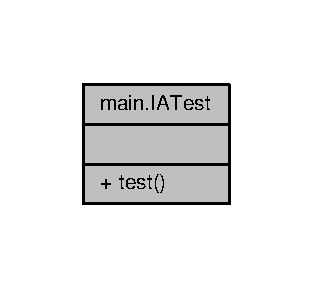
\includegraphics[width=150pt]{classmain_1_1IATest__coll__graph}
\end{center}
\end{figure}
\subsubsection*{Fonctions membres publiques}
\begin{DoxyCompactItemize}
\item 
void \hyperlink{classmain_1_1IATest_a1a855c8a3bcca844bc8adfe44927d4e7}{test} ()  throws A\+W\+T\+Exception 
\end{DoxyCompactItemize}


\subsubsection{Documentation des fonctions membres}
\hypertarget{classmain_1_1IATest_a1a855c8a3bcca844bc8adfe44927d4e7}{}\index{main\+::\+I\+A\+Test@{main\+::\+I\+A\+Test}!test@{test}}
\index{test@{test}!main\+::\+I\+A\+Test@{main\+::\+I\+A\+Test}}
\paragraph[{test}]{\setlength{\rightskip}{0pt plus 5cm}void main.\+I\+A\+Test.\+test (
\begin{DoxyParamCaption}
{}
\end{DoxyParamCaption}
) throws A\+W\+T\+Exception}\label{classmain_1_1IATest_a1a855c8a3bcca844bc8adfe44927d4e7}


La documentation de cette classe a été générée à partir du fichier suivant \+:\begin{DoxyCompactItemize}
\item 
\hyperlink{main_2IATest_8java}{main/\+I\+A\+Test.\+java}\end{DoxyCompactItemize}

\hypertarget{classImageRecognitionTest}{}\subsection{Référence de la classe Image\+Recognition\+Test}
\label{classImageRecognitionTest}\index{Image\+Recognition\+Test@{Image\+Recognition\+Test}}


Graphe de collaboration de Image\+Recognition\+Test\+:\nopagebreak
\begin{figure}[H]
\begin{center}
\leavevmode
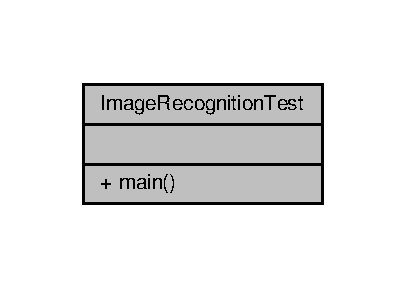
\includegraphics[width=195pt]{classImageRecognitionTest__coll__graph}
\end{center}
\end{figure}
\subsubsection*{Fonctions membres publiques statiques}
\begin{DoxyCompactItemize}
\item 
static void \hyperlink{classImageRecognitionTest_a9b113244821fe71bc603f8c5f3f47e6a}{main} (String\mbox{[}$\,$\mbox{]} args)
\end{DoxyCompactItemize}


\subsubsection{Documentation des fonctions membres}
\hypertarget{classImageRecognitionTest_a9b113244821fe71bc603f8c5f3f47e6a}{}\index{Image\+Recognition\+Test@{Image\+Recognition\+Test}!main@{main}}
\index{main@{main}!Image\+Recognition\+Test@{Image\+Recognition\+Test}}
\paragraph[{main}]{\setlength{\rightskip}{0pt plus 5cm}static void Image\+Recognition\+Test.\+main (
\begin{DoxyParamCaption}
\item[{String\mbox{[}$\,$\mbox{]}}]{args}
\end{DoxyParamCaption}
)\hspace{0.3cm}{\ttfamily [static]}}\label{classImageRecognitionTest_a9b113244821fe71bc603f8c5f3f47e6a}


La documentation de cette classe a été générée à partir du fichier suivant \+:\begin{DoxyCompactItemize}
\item 
\hyperlink{ImageRecognitionTest_8java}{Image\+Recognition\+Test.\+java}\end{DoxyCompactItemize}

\hypertarget{classIMGRecognition}{}\subsection{Référence de la classe I\+M\+G\+Recognition}
\label{classIMGRecognition}\index{I\+M\+G\+Recognition@{I\+M\+G\+Recognition}}


Graphe de collaboration de I\+M\+G\+Recognition\+:\nopagebreak
\begin{figure}[H]
\begin{center}
\leavevmode
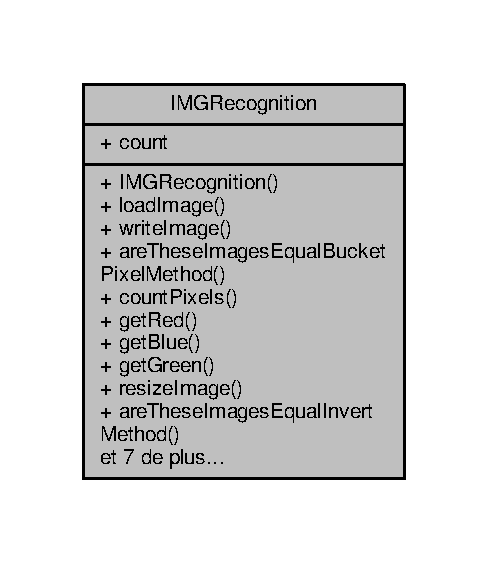
\includegraphics[width=234pt]{classIMGRecognition__coll__graph}
\end{center}
\end{figure}
\subsubsection*{Fonctions membres publiques}
\begin{DoxyCompactItemize}
\item 
\hyperlink{classIMGRecognition_a12b6f92bcc6cf51a70b4299b63dc07c9}{I\+M\+G\+Recognition} ()
\item 
Buffered\+Image \hyperlink{classIMGRecognition_a563c26081c02144dfcc6783886793532}{load\+Image} (String filename)
\item 
void \hyperlink{classIMGRecognition_aeffad758b71b49b25851a5a7f2727de8}{write\+Image} (Buffered\+Image im, String nom)
\item 
Boolean \hyperlink{classIMGRecognition_ab06b57744429b303220659775316f015}{are\+These\+Images\+Equal\+Bucket\+Pixel\+Method} (String name1, String name2, int precision)
\item 
int\mbox{[}$\,$\mbox{]} \hyperlink{classIMGRecognition_a8fad78515c21b2195c0866fbb8e4d348}{count\+Pixels} (Buffered\+Image img, int\mbox{[}$\,$\mbox{]} tab)
\item 
int \hyperlink{classIMGRecognition_ae370d79f59e42f1134776eb7d10a4d5b}{get\+Red} (Buffered\+Image img, int x, int y)
\item 
int \hyperlink{classIMGRecognition_abfc810952febb3c84254ee0e339605cf}{get\+Blue} (Buffered\+Image img, int x, int y)
\item 
int \hyperlink{classIMGRecognition_a4a2c4b182067edf9853b2974fc7d0893}{get\+Green} (Buffered\+Image img, int x, int y)
\item 
Buffered\+Image \hyperlink{classIMGRecognition_a58dea1e82edb9095160cacbb60e74dc4}{resize\+Image} (Buffered\+Image original, int new\+W, int new\+H)
\item 
Boolean \hyperlink{classIMGRecognition_aabdc590dd4a074972106c61b6013f7aa}{are\+These\+Images\+Equal\+Invert\+Method} (String im\+N1, Buffered\+Image im2, int precision)
\item 
Buffered\+Image \hyperlink{classIMGRecognition_a6fe8d29184cea9a3d6492aef6dbe9b8e}{add\+Images} (Buffered\+Image im1, Buffered\+Image im2)
\item 
Buffered\+Image \hyperlink{classIMGRecognition_a58a3b199e12c2f45c5b2841bf7779353}{invert\+Image} (Buffered\+Image img)
\item 
Buffered\+Image \hyperlink{classIMGRecognition_a6bcc57c1f558a08072c8deab1960d479}{set\+Alpha} (Buffered\+Image img, byte alpha)
\item 
Buffered\+Image \hyperlink{classIMGRecognition_a8a767f011a12abbd277e69c36ee6cafc}{set\+R\+G\+B} (Buffered\+Image img, int x, int y, int red, int green, int blue)
\item 
Buffered\+Image \hyperlink{classIMGRecognition_a8528898517213e625355e4de66a22ed0}{set\+R\+G\+Bw\+Alpha} (Buffered\+Image img, int x, int y, int red, int green, int blue, int alpha)
\item 
Boolean \hyperlink{classIMGRecognition_a107ca0380e3816d0a8ed6bf63fbe8e62}{check\+White\+Image} (Buffered\+Image img, int precision)
\item 
Buffered\+Image \hyperlink{classIMGRecognition_a7a4f0c3354c57bb4f9231736cac4295d}{xor\+Effect} (Buffered\+Image image\+A, Buffered\+Image image\+B)
\end{DoxyCompactItemize}
\subsubsection*{Attributs publics statiques}
\begin{DoxyCompactItemize}
\item 
static int \hyperlink{classIMGRecognition_a7ac9e90406c1ef2ef253c1f8b304a308}{count} = 0
\end{DoxyCompactItemize}


\subsubsection{Documentation des constructeurs et destructeur}
\hypertarget{classIMGRecognition_a12b6f92bcc6cf51a70b4299b63dc07c9}{}\index{I\+M\+G\+Recognition@{I\+M\+G\+Recognition}!I\+M\+G\+Recognition@{I\+M\+G\+Recognition}}
\index{I\+M\+G\+Recognition@{I\+M\+G\+Recognition}!I\+M\+G\+Recognition@{I\+M\+G\+Recognition}}
\paragraph[{I\+M\+G\+Recognition}]{\setlength{\rightskip}{0pt plus 5cm}I\+M\+G\+Recognition.\+I\+M\+G\+Recognition (
\begin{DoxyParamCaption}
{}
\end{DoxyParamCaption}
)}\label{classIMGRecognition_a12b6f92bcc6cf51a70b4299b63dc07c9}


\subsubsection{Documentation des fonctions membres}
\hypertarget{classIMGRecognition_a6fe8d29184cea9a3d6492aef6dbe9b8e}{}\index{I\+M\+G\+Recognition@{I\+M\+G\+Recognition}!add\+Images@{add\+Images}}
\index{add\+Images@{add\+Images}!I\+M\+G\+Recognition@{I\+M\+G\+Recognition}}
\paragraph[{add\+Images}]{\setlength{\rightskip}{0pt plus 5cm}Buffered\+Image I\+M\+G\+Recognition.\+add\+Images (
\begin{DoxyParamCaption}
\item[{Buffered\+Image}]{im1, }
\item[{Buffered\+Image}]{im2}
\end{DoxyParamCaption}
)}\label{classIMGRecognition_a6fe8d29184cea9a3d6492aef6dbe9b8e}


Référencé par are\+These\+Images\+Equal\+Invert\+Method().

\hypertarget{classIMGRecognition_ab06b57744429b303220659775316f015}{}\index{I\+M\+G\+Recognition@{I\+M\+G\+Recognition}!are\+These\+Images\+Equal\+Bucket\+Pixel\+Method@{are\+These\+Images\+Equal\+Bucket\+Pixel\+Method}}
\index{are\+These\+Images\+Equal\+Bucket\+Pixel\+Method@{are\+These\+Images\+Equal\+Bucket\+Pixel\+Method}!I\+M\+G\+Recognition@{I\+M\+G\+Recognition}}
\paragraph[{are\+These\+Images\+Equal\+Bucket\+Pixel\+Method}]{\setlength{\rightskip}{0pt plus 5cm}Boolean I\+M\+G\+Recognition.\+are\+These\+Images\+Equal\+Bucket\+Pixel\+Method (
\begin{DoxyParamCaption}
\item[{String}]{name1, }
\item[{String}]{name2, }
\item[{int}]{precision}
\end{DoxyParamCaption}
)}\label{classIMGRecognition_ab06b57744429b303220659775316f015}
\hypertarget{classIMGRecognition_aabdc590dd4a074972106c61b6013f7aa}{}\index{I\+M\+G\+Recognition@{I\+M\+G\+Recognition}!are\+These\+Images\+Equal\+Invert\+Method@{are\+These\+Images\+Equal\+Invert\+Method}}
\index{are\+These\+Images\+Equal\+Invert\+Method@{are\+These\+Images\+Equal\+Invert\+Method}!I\+M\+G\+Recognition@{I\+M\+G\+Recognition}}
\paragraph[{are\+These\+Images\+Equal\+Invert\+Method}]{\setlength{\rightskip}{0pt plus 5cm}Boolean I\+M\+G\+Recognition.\+are\+These\+Images\+Equal\+Invert\+Method (
\begin{DoxyParamCaption}
\item[{String}]{im\+N1, }
\item[{Buffered\+Image}]{im2, }
\item[{int}]{precision}
\end{DoxyParamCaption}
)}\label{classIMGRecognition_aabdc590dd4a074972106c61b6013f7aa}


Référencé par I\+A.\+get\+Sushi().

\hypertarget{classIMGRecognition_a107ca0380e3816d0a8ed6bf63fbe8e62}{}\index{I\+M\+G\+Recognition@{I\+M\+G\+Recognition}!check\+White\+Image@{check\+White\+Image}}
\index{check\+White\+Image@{check\+White\+Image}!I\+M\+G\+Recognition@{I\+M\+G\+Recognition}}
\paragraph[{check\+White\+Image}]{\setlength{\rightskip}{0pt plus 5cm}Boolean I\+M\+G\+Recognition.\+check\+White\+Image (
\begin{DoxyParamCaption}
\item[{Buffered\+Image}]{img, }
\item[{int}]{precision}
\end{DoxyParamCaption}
)}\label{classIMGRecognition_a107ca0380e3816d0a8ed6bf63fbe8e62}


Référencé par are\+These\+Images\+Equal\+Invert\+Method().

\hypertarget{classIMGRecognition_a8fad78515c21b2195c0866fbb8e4d348}{}\index{I\+M\+G\+Recognition@{I\+M\+G\+Recognition}!count\+Pixels@{count\+Pixels}}
\index{count\+Pixels@{count\+Pixels}!I\+M\+G\+Recognition@{I\+M\+G\+Recognition}}
\paragraph[{count\+Pixels}]{\setlength{\rightskip}{0pt plus 5cm}int \mbox{[}$\,$\mbox{]} I\+M\+G\+Recognition.\+count\+Pixels (
\begin{DoxyParamCaption}
\item[{Buffered\+Image}]{img, }
\item[{int\mbox{[}$\,$\mbox{]}}]{tab}
\end{DoxyParamCaption}
)}\label{classIMGRecognition_a8fad78515c21b2195c0866fbb8e4d348}


Référencé par are\+These\+Images\+Equal\+Bucket\+Pixel\+Method().

\hypertarget{classIMGRecognition_abfc810952febb3c84254ee0e339605cf}{}\index{I\+M\+G\+Recognition@{I\+M\+G\+Recognition}!get\+Blue@{get\+Blue}}
\index{get\+Blue@{get\+Blue}!I\+M\+G\+Recognition@{I\+M\+G\+Recognition}}
\paragraph[{get\+Blue}]{\setlength{\rightskip}{0pt plus 5cm}int I\+M\+G\+Recognition.\+get\+Blue (
\begin{DoxyParamCaption}
\item[{Buffered\+Image}]{img, }
\item[{int}]{x, }
\item[{int}]{y}
\end{DoxyParamCaption}
)}\label{classIMGRecognition_abfc810952febb3c84254ee0e339605cf}


Référencé par add\+Images(), check\+White\+Image(), et count\+Pixels().

\hypertarget{classIMGRecognition_a4a2c4b182067edf9853b2974fc7d0893}{}\index{I\+M\+G\+Recognition@{I\+M\+G\+Recognition}!get\+Green@{get\+Green}}
\index{get\+Green@{get\+Green}!I\+M\+G\+Recognition@{I\+M\+G\+Recognition}}
\paragraph[{get\+Green}]{\setlength{\rightskip}{0pt plus 5cm}int I\+M\+G\+Recognition.\+get\+Green (
\begin{DoxyParamCaption}
\item[{Buffered\+Image}]{img, }
\item[{int}]{x, }
\item[{int}]{y}
\end{DoxyParamCaption}
)}\label{classIMGRecognition_a4a2c4b182067edf9853b2974fc7d0893}


Référencé par add\+Images(), check\+White\+Image(), et count\+Pixels().

\hypertarget{classIMGRecognition_ae370d79f59e42f1134776eb7d10a4d5b}{}\index{I\+M\+G\+Recognition@{I\+M\+G\+Recognition}!get\+Red@{get\+Red}}
\index{get\+Red@{get\+Red}!I\+M\+G\+Recognition@{I\+M\+G\+Recognition}}
\paragraph[{get\+Red}]{\setlength{\rightskip}{0pt plus 5cm}int I\+M\+G\+Recognition.\+get\+Red (
\begin{DoxyParamCaption}
\item[{Buffered\+Image}]{img, }
\item[{int}]{x, }
\item[{int}]{y}
\end{DoxyParamCaption}
)}\label{classIMGRecognition_ae370d79f59e42f1134776eb7d10a4d5b}


Référencé par add\+Images(), check\+White\+Image(), et count\+Pixels().

\hypertarget{classIMGRecognition_a58a3b199e12c2f45c5b2841bf7779353}{}\index{I\+M\+G\+Recognition@{I\+M\+G\+Recognition}!invert\+Image@{invert\+Image}}
\index{invert\+Image@{invert\+Image}!I\+M\+G\+Recognition@{I\+M\+G\+Recognition}}
\paragraph[{invert\+Image}]{\setlength{\rightskip}{0pt plus 5cm}Buffered\+Image I\+M\+G\+Recognition.\+invert\+Image (
\begin{DoxyParamCaption}
\item[{Buffered\+Image}]{img}
\end{DoxyParamCaption}
)}\label{classIMGRecognition_a58a3b199e12c2f45c5b2841bf7779353}


Référencé par are\+These\+Images\+Equal\+Invert\+Method().

\hypertarget{classIMGRecognition_a563c26081c02144dfcc6783886793532}{}\index{I\+M\+G\+Recognition@{I\+M\+G\+Recognition}!load\+Image@{load\+Image}}
\index{load\+Image@{load\+Image}!I\+M\+G\+Recognition@{I\+M\+G\+Recognition}}
\paragraph[{load\+Image}]{\setlength{\rightskip}{0pt plus 5cm}Buffered\+Image I\+M\+G\+Recognition.\+load\+Image (
\begin{DoxyParamCaption}
\item[{String}]{filename}
\end{DoxyParamCaption}
)}\label{classIMGRecognition_a563c26081c02144dfcc6783886793532}


Référencé par are\+These\+Images\+Equal\+Bucket\+Pixel\+Method(), are\+These\+Images\+Equal\+Invert\+Method(), et I\+M\+G\+Recognition\+Test.\+test().

\hypertarget{classIMGRecognition_a58dea1e82edb9095160cacbb60e74dc4}{}\index{I\+M\+G\+Recognition@{I\+M\+G\+Recognition}!resize\+Image@{resize\+Image}}
\index{resize\+Image@{resize\+Image}!I\+M\+G\+Recognition@{I\+M\+G\+Recognition}}
\paragraph[{resize\+Image}]{\setlength{\rightskip}{0pt plus 5cm}Buffered\+Image I\+M\+G\+Recognition.\+resize\+Image (
\begin{DoxyParamCaption}
\item[{Buffered\+Image}]{original, }
\item[{int}]{new\+W, }
\item[{int}]{new\+H}
\end{DoxyParamCaption}
)}\label{classIMGRecognition_a58dea1e82edb9095160cacbb60e74dc4}
\hypertarget{classIMGRecognition_a6bcc57c1f558a08072c8deab1960d479}{}\index{I\+M\+G\+Recognition@{I\+M\+G\+Recognition}!set\+Alpha@{set\+Alpha}}
\index{set\+Alpha@{set\+Alpha}!I\+M\+G\+Recognition@{I\+M\+G\+Recognition}}
\paragraph[{set\+Alpha}]{\setlength{\rightskip}{0pt plus 5cm}Buffered\+Image I\+M\+G\+Recognition.\+set\+Alpha (
\begin{DoxyParamCaption}
\item[{Buffered\+Image}]{img, }
\item[{byte}]{alpha}
\end{DoxyParamCaption}
)}\label{classIMGRecognition_a6bcc57c1f558a08072c8deab1960d479}


Référencé par invert\+Image().

\hypertarget{classIMGRecognition_a8a767f011a12abbd277e69c36ee6cafc}{}\index{I\+M\+G\+Recognition@{I\+M\+G\+Recognition}!set\+R\+G\+B@{set\+R\+G\+B}}
\index{set\+R\+G\+B@{set\+R\+G\+B}!I\+M\+G\+Recognition@{I\+M\+G\+Recognition}}
\paragraph[{set\+R\+G\+B}]{\setlength{\rightskip}{0pt plus 5cm}Buffered\+Image I\+M\+G\+Recognition.\+set\+R\+G\+B (
\begin{DoxyParamCaption}
\item[{Buffered\+Image}]{img, }
\item[{int}]{x, }
\item[{int}]{y, }
\item[{int}]{red, }
\item[{int}]{green, }
\item[{int}]{blue}
\end{DoxyParamCaption}
)}\label{classIMGRecognition_a8a767f011a12abbd277e69c36ee6cafc}


Référencé par add\+Images().

\hypertarget{classIMGRecognition_a8528898517213e625355e4de66a22ed0}{}\index{I\+M\+G\+Recognition@{I\+M\+G\+Recognition}!set\+R\+G\+Bw\+Alpha@{set\+R\+G\+Bw\+Alpha}}
\index{set\+R\+G\+Bw\+Alpha@{set\+R\+G\+Bw\+Alpha}!I\+M\+G\+Recognition@{I\+M\+G\+Recognition}}
\paragraph[{set\+R\+G\+Bw\+Alpha}]{\setlength{\rightskip}{0pt plus 5cm}Buffered\+Image I\+M\+G\+Recognition.\+set\+R\+G\+Bw\+Alpha (
\begin{DoxyParamCaption}
\item[{Buffered\+Image}]{img, }
\item[{int}]{x, }
\item[{int}]{y, }
\item[{int}]{red, }
\item[{int}]{green, }
\item[{int}]{blue, }
\item[{int}]{alpha}
\end{DoxyParamCaption}
)}\label{classIMGRecognition_a8528898517213e625355e4de66a22ed0}
\hypertarget{classIMGRecognition_aeffad758b71b49b25851a5a7f2727de8}{}\index{I\+M\+G\+Recognition@{I\+M\+G\+Recognition}!write\+Image@{write\+Image}}
\index{write\+Image@{write\+Image}!I\+M\+G\+Recognition@{I\+M\+G\+Recognition}}
\paragraph[{write\+Image}]{\setlength{\rightskip}{0pt plus 5cm}void I\+M\+G\+Recognition.\+write\+Image (
\begin{DoxyParamCaption}
\item[{Buffered\+Image}]{im, }
\item[{String}]{nom}
\end{DoxyParamCaption}
)}\label{classIMGRecognition_aeffad758b71b49b25851a5a7f2727de8}


Référencé par are\+These\+Images\+Equal\+Invert\+Method(), et I\+M\+G\+Recognition\+Test.\+test().

\hypertarget{classIMGRecognition_a7a4f0c3354c57bb4f9231736cac4295d}{}\index{I\+M\+G\+Recognition@{I\+M\+G\+Recognition}!xor\+Effect@{xor\+Effect}}
\index{xor\+Effect@{xor\+Effect}!I\+M\+G\+Recognition@{I\+M\+G\+Recognition}}
\paragraph[{xor\+Effect}]{\setlength{\rightskip}{0pt plus 5cm}Buffered\+Image I\+M\+G\+Recognition.\+xor\+Effect (
\begin{DoxyParamCaption}
\item[{Buffered\+Image}]{image\+A, }
\item[{Buffered\+Image}]{image\+B}
\end{DoxyParamCaption}
)}\label{classIMGRecognition_a7a4f0c3354c57bb4f9231736cac4295d}


Référencé par I\+M\+G\+Recognition\+Test.\+test().



\subsubsection{Documentation des données membres}
\hypertarget{classIMGRecognition_a7ac9e90406c1ef2ef253c1f8b304a308}{}\index{I\+M\+G\+Recognition@{I\+M\+G\+Recognition}!count@{count}}
\index{count@{count}!I\+M\+G\+Recognition@{I\+M\+G\+Recognition}}
\paragraph[{count}]{\setlength{\rightskip}{0pt plus 5cm}int I\+M\+G\+Recognition.\+count = 0\hspace{0.3cm}{\ttfamily [static]}}\label{classIMGRecognition_a7ac9e90406c1ef2ef253c1f8b304a308}


La documentation de cette classe a été générée à partir du fichier suivant \+:\begin{DoxyCompactItemize}
\item 
\hyperlink{oldCode_2IMGRecognition_8java}{old\+Code/\+I\+M\+G\+Recognition.\+java}\end{DoxyCompactItemize}

\hypertarget{classmain_1_1IMGRecognition}{}\subsection{Référence de la classe main.\+I\+M\+G\+Recognition}
\label{classmain_1_1IMGRecognition}\index{main.\+I\+M\+G\+Recognition@{main.\+I\+M\+G\+Recognition}}


Graphe de collaboration de main.\+I\+M\+G\+Recognition\+:\nopagebreak
\begin{figure}[H]
\begin{center}
\leavevmode
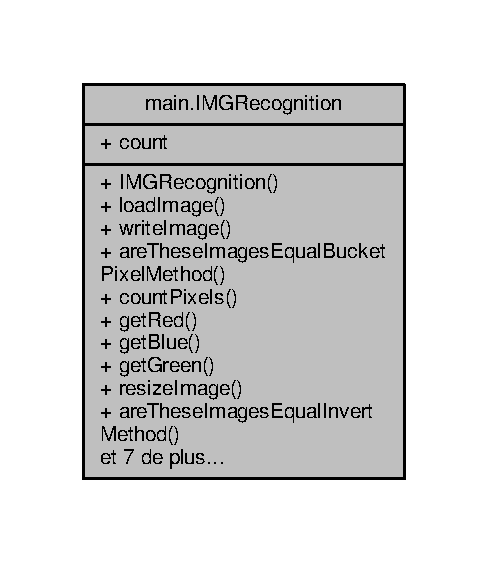
\includegraphics[width=234pt]{classmain_1_1IMGRecognition__coll__graph}
\end{center}
\end{figure}
\subsubsection*{Fonctions membres publiques}
\begin{DoxyCompactItemize}
\item 
\hyperlink{classmain_1_1IMGRecognition_ad3a4c7df4f9a57b7b651ec87432f7427}{I\+M\+G\+Recognition} ()
\item 
Buffered\+Image \hyperlink{classmain_1_1IMGRecognition_aaa715f046dad799280c48bf91abed47e}{load\+Image} (String filename)
\item 
void \hyperlink{classmain_1_1IMGRecognition_ad08ec39dbf190463dade62d96fcb3809}{write\+Image} (Buffered\+Image im, String nom)
\item 
Boolean \hyperlink{classmain_1_1IMGRecognition_a9c1b15071aec2401dbcd196089bf0410}{are\+These\+Images\+Equal\+Bucket\+Pixel\+Method} (String name1, String name2, int precision)
\item 
int\mbox{[}$\,$\mbox{]} \hyperlink{classmain_1_1IMGRecognition_a485c324e088c83d9b14e73a3d2b31bf7}{count\+Pixels} (Buffered\+Image img, int\mbox{[}$\,$\mbox{]} tab)
\item 
int \hyperlink{classmain_1_1IMGRecognition_a081b6ae5204140c4cb0da69e181cf334}{get\+Red} (Buffered\+Image img, int x, int y)
\item 
int \hyperlink{classmain_1_1IMGRecognition_a35e1dab265347a43b66b0b023b0205c4}{get\+Blue} (Buffered\+Image img, int x, int y)
\item 
int \hyperlink{classmain_1_1IMGRecognition_abf7642a1359d08a759c0e36fd8b9f0d2}{get\+Green} (Buffered\+Image img, int x, int y)
\item 
Buffered\+Image \hyperlink{classmain_1_1IMGRecognition_ab370e4f70a8a19a9cdcbc8972bc3e86f}{resize\+Image} (Buffered\+Image original, int new\+W, int new\+H)
\item 
Boolean \hyperlink{classmain_1_1IMGRecognition_ad83e42f0ca9930d8b14ebe859e508241}{are\+These\+Images\+Equal\+Invert\+Method} (String im\+N1, Buffered\+Image im2, int precision)
\item 
Buffered\+Image \hyperlink{classmain_1_1IMGRecognition_a82048c15daa3bbb8e930b0af41c96fb4}{add\+Images} (Buffered\+Image im1, Buffered\+Image im2)
\item 
Buffered\+Image \hyperlink{classmain_1_1IMGRecognition_ac3c82596f3127a48f0093b479ee9d450}{invert\+Image} (Buffered\+Image img)
\item 
Buffered\+Image \hyperlink{classmain_1_1IMGRecognition_aba224b9de06ccbcd28bed1fb041ca336}{set\+Alpha} (Buffered\+Image img, byte alpha)
\item 
Buffered\+Image \hyperlink{classmain_1_1IMGRecognition_a7d21c03134b7a5de78a8a8e7a3daf2ca}{set\+R\+G\+B} (Buffered\+Image img, int x, int y, int red, int green, int blue)
\item 
Buffered\+Image \hyperlink{classmain_1_1IMGRecognition_a68fbe2297ec670f69a1f009ec612bdd0}{set\+R\+G\+Bw\+Alpha} (Buffered\+Image img, int x, int y, int red, int green, int blue, int alpha)
\item 
Boolean \hyperlink{classmain_1_1IMGRecognition_ab50b61f6d13b47900123d07ac10566b9}{check\+White\+Image} (Buffered\+Image img, int precision)
\item 
Buffered\+Image \hyperlink{classmain_1_1IMGRecognition_ae8a26863347c7800607fe78e1f3e84ee}{xor\+Effect} (Buffered\+Image image\+A, Buffered\+Image image\+B)
\end{DoxyCompactItemize}
\subsubsection*{Attributs publics statiques}
\begin{DoxyCompactItemize}
\item 
static int \hyperlink{classmain_1_1IMGRecognition_a5caedac76054d4d70d3fbc142c3fcf1b}{count} = 0
\end{DoxyCompactItemize}


\subsubsection{Documentation des constructeurs et destructeur}
\hypertarget{classmain_1_1IMGRecognition_ad3a4c7df4f9a57b7b651ec87432f7427}{}\index{main\+::\+I\+M\+G\+Recognition@{main\+::\+I\+M\+G\+Recognition}!I\+M\+G\+Recognition@{I\+M\+G\+Recognition}}
\index{I\+M\+G\+Recognition@{I\+M\+G\+Recognition}!main\+::\+I\+M\+G\+Recognition@{main\+::\+I\+M\+G\+Recognition}}
\paragraph[{I\+M\+G\+Recognition}]{\setlength{\rightskip}{0pt plus 5cm}main.\+I\+M\+G\+Recognition.\+I\+M\+G\+Recognition (
\begin{DoxyParamCaption}
{}
\end{DoxyParamCaption}
)}\label{classmain_1_1IMGRecognition_ad3a4c7df4f9a57b7b651ec87432f7427}


\subsubsection{Documentation des fonctions membres}
\hypertarget{classmain_1_1IMGRecognition_a82048c15daa3bbb8e930b0af41c96fb4}{}\index{main\+::\+I\+M\+G\+Recognition@{main\+::\+I\+M\+G\+Recognition}!add\+Images@{add\+Images}}
\index{add\+Images@{add\+Images}!main\+::\+I\+M\+G\+Recognition@{main\+::\+I\+M\+G\+Recognition}}
\paragraph[{add\+Images}]{\setlength{\rightskip}{0pt plus 5cm}Buffered\+Image main.\+I\+M\+G\+Recognition.\+add\+Images (
\begin{DoxyParamCaption}
\item[{Buffered\+Image}]{im1, }
\item[{Buffered\+Image}]{im2}
\end{DoxyParamCaption}
)}\label{classmain_1_1IMGRecognition_a82048c15daa3bbb8e930b0af41c96fb4}


Référencé par main.\+I\+M\+G\+Recognition.\+are\+These\+Images\+Equal\+Invert\+Method().

\hypertarget{classmain_1_1IMGRecognition_a9c1b15071aec2401dbcd196089bf0410}{}\index{main\+::\+I\+M\+G\+Recognition@{main\+::\+I\+M\+G\+Recognition}!are\+These\+Images\+Equal\+Bucket\+Pixel\+Method@{are\+These\+Images\+Equal\+Bucket\+Pixel\+Method}}
\index{are\+These\+Images\+Equal\+Bucket\+Pixel\+Method@{are\+These\+Images\+Equal\+Bucket\+Pixel\+Method}!main\+::\+I\+M\+G\+Recognition@{main\+::\+I\+M\+G\+Recognition}}
\paragraph[{are\+These\+Images\+Equal\+Bucket\+Pixel\+Method}]{\setlength{\rightskip}{0pt plus 5cm}Boolean main.\+I\+M\+G\+Recognition.\+are\+These\+Images\+Equal\+Bucket\+Pixel\+Method (
\begin{DoxyParamCaption}
\item[{String}]{name1, }
\item[{String}]{name2, }
\item[{int}]{precision}
\end{DoxyParamCaption}
)}\label{classmain_1_1IMGRecognition_a9c1b15071aec2401dbcd196089bf0410}
\hypertarget{classmain_1_1IMGRecognition_ad83e42f0ca9930d8b14ebe859e508241}{}\index{main\+::\+I\+M\+G\+Recognition@{main\+::\+I\+M\+G\+Recognition}!are\+These\+Images\+Equal\+Invert\+Method@{are\+These\+Images\+Equal\+Invert\+Method}}
\index{are\+These\+Images\+Equal\+Invert\+Method@{are\+These\+Images\+Equal\+Invert\+Method}!main\+::\+I\+M\+G\+Recognition@{main\+::\+I\+M\+G\+Recognition}}
\paragraph[{are\+These\+Images\+Equal\+Invert\+Method}]{\setlength{\rightskip}{0pt plus 5cm}Boolean main.\+I\+M\+G\+Recognition.\+are\+These\+Images\+Equal\+Invert\+Method (
\begin{DoxyParamCaption}
\item[{String}]{im\+N1, }
\item[{Buffered\+Image}]{im2, }
\item[{int}]{precision}
\end{DoxyParamCaption}
)}\label{classmain_1_1IMGRecognition_ad83e42f0ca9930d8b14ebe859e508241}


Référencé par main.\+I\+A.\+get\+Sushi().

\hypertarget{classmain_1_1IMGRecognition_ab50b61f6d13b47900123d07ac10566b9}{}\index{main\+::\+I\+M\+G\+Recognition@{main\+::\+I\+M\+G\+Recognition}!check\+White\+Image@{check\+White\+Image}}
\index{check\+White\+Image@{check\+White\+Image}!main\+::\+I\+M\+G\+Recognition@{main\+::\+I\+M\+G\+Recognition}}
\paragraph[{check\+White\+Image}]{\setlength{\rightskip}{0pt plus 5cm}Boolean main.\+I\+M\+G\+Recognition.\+check\+White\+Image (
\begin{DoxyParamCaption}
\item[{Buffered\+Image}]{img, }
\item[{int}]{precision}
\end{DoxyParamCaption}
)}\label{classmain_1_1IMGRecognition_ab50b61f6d13b47900123d07ac10566b9}


Référencé par main.\+I\+M\+G\+Recognition.\+are\+These\+Images\+Equal\+Invert\+Method().

\hypertarget{classmain_1_1IMGRecognition_a485c324e088c83d9b14e73a3d2b31bf7}{}\index{main\+::\+I\+M\+G\+Recognition@{main\+::\+I\+M\+G\+Recognition}!count\+Pixels@{count\+Pixels}}
\index{count\+Pixels@{count\+Pixels}!main\+::\+I\+M\+G\+Recognition@{main\+::\+I\+M\+G\+Recognition}}
\paragraph[{count\+Pixels}]{\setlength{\rightskip}{0pt plus 5cm}int \mbox{[}$\,$\mbox{]} main.\+I\+M\+G\+Recognition.\+count\+Pixels (
\begin{DoxyParamCaption}
\item[{Buffered\+Image}]{img, }
\item[{int\mbox{[}$\,$\mbox{]}}]{tab}
\end{DoxyParamCaption}
)}\label{classmain_1_1IMGRecognition_a485c324e088c83d9b14e73a3d2b31bf7}


Référencé par main.\+I\+M\+G\+Recognition.\+are\+These\+Images\+Equal\+Bucket\+Pixel\+Method().

\hypertarget{classmain_1_1IMGRecognition_a35e1dab265347a43b66b0b023b0205c4}{}\index{main\+::\+I\+M\+G\+Recognition@{main\+::\+I\+M\+G\+Recognition}!get\+Blue@{get\+Blue}}
\index{get\+Blue@{get\+Blue}!main\+::\+I\+M\+G\+Recognition@{main\+::\+I\+M\+G\+Recognition}}
\paragraph[{get\+Blue}]{\setlength{\rightskip}{0pt plus 5cm}int main.\+I\+M\+G\+Recognition.\+get\+Blue (
\begin{DoxyParamCaption}
\item[{Buffered\+Image}]{img, }
\item[{int}]{x, }
\item[{int}]{y}
\end{DoxyParamCaption}
)}\label{classmain_1_1IMGRecognition_a35e1dab265347a43b66b0b023b0205c4}


Référencé par main.\+I\+M\+G\+Recognition.\+add\+Images(), main.\+I\+M\+G\+Recognition.\+check\+White\+Image(), et main.\+I\+M\+G\+Recognition.\+count\+Pixels().

\hypertarget{classmain_1_1IMGRecognition_abf7642a1359d08a759c0e36fd8b9f0d2}{}\index{main\+::\+I\+M\+G\+Recognition@{main\+::\+I\+M\+G\+Recognition}!get\+Green@{get\+Green}}
\index{get\+Green@{get\+Green}!main\+::\+I\+M\+G\+Recognition@{main\+::\+I\+M\+G\+Recognition}}
\paragraph[{get\+Green}]{\setlength{\rightskip}{0pt plus 5cm}int main.\+I\+M\+G\+Recognition.\+get\+Green (
\begin{DoxyParamCaption}
\item[{Buffered\+Image}]{img, }
\item[{int}]{x, }
\item[{int}]{y}
\end{DoxyParamCaption}
)}\label{classmain_1_1IMGRecognition_abf7642a1359d08a759c0e36fd8b9f0d2}


Référencé par main.\+I\+M\+G\+Recognition.\+add\+Images(), main.\+I\+M\+G\+Recognition.\+check\+White\+Image(), et main.\+I\+M\+G\+Recognition.\+count\+Pixels().

\hypertarget{classmain_1_1IMGRecognition_a081b6ae5204140c4cb0da69e181cf334}{}\index{main\+::\+I\+M\+G\+Recognition@{main\+::\+I\+M\+G\+Recognition}!get\+Red@{get\+Red}}
\index{get\+Red@{get\+Red}!main\+::\+I\+M\+G\+Recognition@{main\+::\+I\+M\+G\+Recognition}}
\paragraph[{get\+Red}]{\setlength{\rightskip}{0pt plus 5cm}int main.\+I\+M\+G\+Recognition.\+get\+Red (
\begin{DoxyParamCaption}
\item[{Buffered\+Image}]{img, }
\item[{int}]{x, }
\item[{int}]{y}
\end{DoxyParamCaption}
)}\label{classmain_1_1IMGRecognition_a081b6ae5204140c4cb0da69e181cf334}


Référencé par main.\+I\+M\+G\+Recognition.\+add\+Images(), main.\+I\+M\+G\+Recognition.\+check\+White\+Image(), et main.\+I\+M\+G\+Recognition.\+count\+Pixels().

\hypertarget{classmain_1_1IMGRecognition_ac3c82596f3127a48f0093b479ee9d450}{}\index{main\+::\+I\+M\+G\+Recognition@{main\+::\+I\+M\+G\+Recognition}!invert\+Image@{invert\+Image}}
\index{invert\+Image@{invert\+Image}!main\+::\+I\+M\+G\+Recognition@{main\+::\+I\+M\+G\+Recognition}}
\paragraph[{invert\+Image}]{\setlength{\rightskip}{0pt plus 5cm}Buffered\+Image main.\+I\+M\+G\+Recognition.\+invert\+Image (
\begin{DoxyParamCaption}
\item[{Buffered\+Image}]{img}
\end{DoxyParamCaption}
)}\label{classmain_1_1IMGRecognition_ac3c82596f3127a48f0093b479ee9d450}


Référencé par main.\+I\+M\+G\+Recognition.\+are\+These\+Images\+Equal\+Invert\+Method().

\hypertarget{classmain_1_1IMGRecognition_aaa715f046dad799280c48bf91abed47e}{}\index{main\+::\+I\+M\+G\+Recognition@{main\+::\+I\+M\+G\+Recognition}!load\+Image@{load\+Image}}
\index{load\+Image@{load\+Image}!main\+::\+I\+M\+G\+Recognition@{main\+::\+I\+M\+G\+Recognition}}
\paragraph[{load\+Image}]{\setlength{\rightskip}{0pt plus 5cm}Buffered\+Image main.\+I\+M\+G\+Recognition.\+load\+Image (
\begin{DoxyParamCaption}
\item[{String}]{filename}
\end{DoxyParamCaption}
)}\label{classmain_1_1IMGRecognition_aaa715f046dad799280c48bf91abed47e}


Référencé par main.\+I\+M\+G\+Recognition.\+are\+These\+Images\+Equal\+Bucket\+Pixel\+Method(), main.\+I\+M\+G\+Recognition.\+are\+These\+Images\+Equal\+Invert\+Method(), et main.\+I\+M\+G\+Recognition\+Test.\+test().

\hypertarget{classmain_1_1IMGRecognition_ab370e4f70a8a19a9cdcbc8972bc3e86f}{}\index{main\+::\+I\+M\+G\+Recognition@{main\+::\+I\+M\+G\+Recognition}!resize\+Image@{resize\+Image}}
\index{resize\+Image@{resize\+Image}!main\+::\+I\+M\+G\+Recognition@{main\+::\+I\+M\+G\+Recognition}}
\paragraph[{resize\+Image}]{\setlength{\rightskip}{0pt plus 5cm}Buffered\+Image main.\+I\+M\+G\+Recognition.\+resize\+Image (
\begin{DoxyParamCaption}
\item[{Buffered\+Image}]{original, }
\item[{int}]{new\+W, }
\item[{int}]{new\+H}
\end{DoxyParamCaption}
)}\label{classmain_1_1IMGRecognition_ab370e4f70a8a19a9cdcbc8972bc3e86f}
\hypertarget{classmain_1_1IMGRecognition_aba224b9de06ccbcd28bed1fb041ca336}{}\index{main\+::\+I\+M\+G\+Recognition@{main\+::\+I\+M\+G\+Recognition}!set\+Alpha@{set\+Alpha}}
\index{set\+Alpha@{set\+Alpha}!main\+::\+I\+M\+G\+Recognition@{main\+::\+I\+M\+G\+Recognition}}
\paragraph[{set\+Alpha}]{\setlength{\rightskip}{0pt plus 5cm}Buffered\+Image main.\+I\+M\+G\+Recognition.\+set\+Alpha (
\begin{DoxyParamCaption}
\item[{Buffered\+Image}]{img, }
\item[{byte}]{alpha}
\end{DoxyParamCaption}
)}\label{classmain_1_1IMGRecognition_aba224b9de06ccbcd28bed1fb041ca336}


Référencé par main.\+I\+M\+G\+Recognition.\+invert\+Image().

\hypertarget{classmain_1_1IMGRecognition_a7d21c03134b7a5de78a8a8e7a3daf2ca}{}\index{main\+::\+I\+M\+G\+Recognition@{main\+::\+I\+M\+G\+Recognition}!set\+R\+G\+B@{set\+R\+G\+B}}
\index{set\+R\+G\+B@{set\+R\+G\+B}!main\+::\+I\+M\+G\+Recognition@{main\+::\+I\+M\+G\+Recognition}}
\paragraph[{set\+R\+G\+B}]{\setlength{\rightskip}{0pt plus 5cm}Buffered\+Image main.\+I\+M\+G\+Recognition.\+set\+R\+G\+B (
\begin{DoxyParamCaption}
\item[{Buffered\+Image}]{img, }
\item[{int}]{x, }
\item[{int}]{y, }
\item[{int}]{red, }
\item[{int}]{green, }
\item[{int}]{blue}
\end{DoxyParamCaption}
)}\label{classmain_1_1IMGRecognition_a7d21c03134b7a5de78a8a8e7a3daf2ca}


Référencé par main.\+I\+M\+G\+Recognition.\+add\+Images().

\hypertarget{classmain_1_1IMGRecognition_a68fbe2297ec670f69a1f009ec612bdd0}{}\index{main\+::\+I\+M\+G\+Recognition@{main\+::\+I\+M\+G\+Recognition}!set\+R\+G\+Bw\+Alpha@{set\+R\+G\+Bw\+Alpha}}
\index{set\+R\+G\+Bw\+Alpha@{set\+R\+G\+Bw\+Alpha}!main\+::\+I\+M\+G\+Recognition@{main\+::\+I\+M\+G\+Recognition}}
\paragraph[{set\+R\+G\+Bw\+Alpha}]{\setlength{\rightskip}{0pt plus 5cm}Buffered\+Image main.\+I\+M\+G\+Recognition.\+set\+R\+G\+Bw\+Alpha (
\begin{DoxyParamCaption}
\item[{Buffered\+Image}]{img, }
\item[{int}]{x, }
\item[{int}]{y, }
\item[{int}]{red, }
\item[{int}]{green, }
\item[{int}]{blue, }
\item[{int}]{alpha}
\end{DoxyParamCaption}
)}\label{classmain_1_1IMGRecognition_a68fbe2297ec670f69a1f009ec612bdd0}
\hypertarget{classmain_1_1IMGRecognition_ad08ec39dbf190463dade62d96fcb3809}{}\index{main\+::\+I\+M\+G\+Recognition@{main\+::\+I\+M\+G\+Recognition}!write\+Image@{write\+Image}}
\index{write\+Image@{write\+Image}!main\+::\+I\+M\+G\+Recognition@{main\+::\+I\+M\+G\+Recognition}}
\paragraph[{write\+Image}]{\setlength{\rightskip}{0pt plus 5cm}void main.\+I\+M\+G\+Recognition.\+write\+Image (
\begin{DoxyParamCaption}
\item[{Buffered\+Image}]{im, }
\item[{String}]{nom}
\end{DoxyParamCaption}
)}\label{classmain_1_1IMGRecognition_ad08ec39dbf190463dade62d96fcb3809}


Référencé par main.\+I\+M\+G\+Recognition.\+are\+These\+Images\+Equal\+Invert\+Method(), main.\+Manager.\+Check\+Bar(), et main.\+I\+M\+G\+Recognition\+Test.\+test().

\hypertarget{classmain_1_1IMGRecognition_ae8a26863347c7800607fe78e1f3e84ee}{}\index{main\+::\+I\+M\+G\+Recognition@{main\+::\+I\+M\+G\+Recognition}!xor\+Effect@{xor\+Effect}}
\index{xor\+Effect@{xor\+Effect}!main\+::\+I\+M\+G\+Recognition@{main\+::\+I\+M\+G\+Recognition}}
\paragraph[{xor\+Effect}]{\setlength{\rightskip}{0pt plus 5cm}Buffered\+Image main.\+I\+M\+G\+Recognition.\+xor\+Effect (
\begin{DoxyParamCaption}
\item[{Buffered\+Image}]{image\+A, }
\item[{Buffered\+Image}]{image\+B}
\end{DoxyParamCaption}
)}\label{classmain_1_1IMGRecognition_ae8a26863347c7800607fe78e1f3e84ee}


Référencé par main.\+I\+M\+G\+Recognition\+Test.\+test().



\subsubsection{Documentation des données membres}
\hypertarget{classmain_1_1IMGRecognition_a5caedac76054d4d70d3fbc142c3fcf1b}{}\index{main\+::\+I\+M\+G\+Recognition@{main\+::\+I\+M\+G\+Recognition}!count@{count}}
\index{count@{count}!main\+::\+I\+M\+G\+Recognition@{main\+::\+I\+M\+G\+Recognition}}
\paragraph[{count}]{\setlength{\rightskip}{0pt plus 5cm}int main.\+I\+M\+G\+Recognition.\+count = 0\hspace{0.3cm}{\ttfamily [static]}}\label{classmain_1_1IMGRecognition_a5caedac76054d4d70d3fbc142c3fcf1b}


La documentation de cette classe a été générée à partir du fichier suivant \+:\begin{DoxyCompactItemize}
\item 
\hyperlink{main_2IMGRecognition_8java}{main/\+I\+M\+G\+Recognition.\+java}\end{DoxyCompactItemize}

\hypertarget{classSushis_1_1src_1_1IMGRecognition}{}\subsection{Référence de la classe Sushis.\+src.\+I\+M\+G\+Recognition}
\label{classSushis_1_1src_1_1IMGRecognition}\index{Sushis.\+src.\+I\+M\+G\+Recognition@{Sushis.\+src.\+I\+M\+G\+Recognition}}


Graphe de collaboration de Sushis.\+src.\+I\+M\+G\+Recognition\+:\nopagebreak
\begin{figure}[H]
\begin{center}
\leavevmode
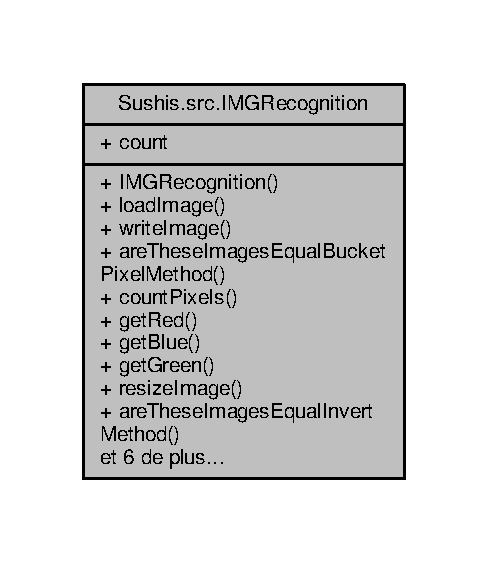
\includegraphics[width=234pt]{classSushis_1_1src_1_1IMGRecognition__coll__graph}
\end{center}
\end{figure}
\subsubsection*{Fonctions membres publiques}
\begin{DoxyCompactItemize}
\item 
\hyperlink{classSushis_1_1src_1_1IMGRecognition_a3e643391bca697087339219b2ed8e2b1}{I\+M\+G\+Recognition} ()
\item 
Buffered\+Image \hyperlink{classSushis_1_1src_1_1IMGRecognition_a4bda2ca4d0b148344c08a8cc392a8de2}{load\+Image} (String filename)
\item 
void \hyperlink{classSushis_1_1src_1_1IMGRecognition_a6b81e073262c0a3aba8cd5adacdc24c0}{write\+Image} (Buffered\+Image im, String nom)
\item 
Boolean \hyperlink{classSushis_1_1src_1_1IMGRecognition_aa23d51110d018fd7f6fa7bb6070c7005}{are\+These\+Images\+Equal\+Bucket\+Pixel\+Method} (String name1, String name2, int precision)
\item 
int\mbox{[}$\,$\mbox{]} \hyperlink{classSushis_1_1src_1_1IMGRecognition_a57521884f4791a8414bafcaaf2e5a2cf}{count\+Pixels} (Buffered\+Image img, int\mbox{[}$\,$\mbox{]} tab)
\item 
int \hyperlink{classSushis_1_1src_1_1IMGRecognition_a0b9590573b448f8cca730f5e827af4b1}{get\+Red} (Buffered\+Image img, int x, int y)
\item 
int \hyperlink{classSushis_1_1src_1_1IMGRecognition_a26b781582f2f88a53a32d2fce1d99f06}{get\+Blue} (Buffered\+Image img, int x, int y)
\item 
int \hyperlink{classSushis_1_1src_1_1IMGRecognition_a920a76c8c0ab2d709b0dfac93ffb4000}{get\+Green} (Buffered\+Image img, int x, int y)
\item 
Buffered\+Image \hyperlink{classSushis_1_1src_1_1IMGRecognition_aa7fb8c8dad7f7ae03b4fea4018b4e5d3}{resize\+Image} (Buffered\+Image original, int new\+W, int new\+H)
\item 
Boolean \hyperlink{classSushis_1_1src_1_1IMGRecognition_a28191e9c0104ffbb4b8d8d4f227b86d3}{are\+These\+Images\+Equal\+Invert\+Method} (String im\+N1, Buffered\+Image im2, int precision)
\item 
Buffered\+Image \hyperlink{classSushis_1_1src_1_1IMGRecognition_aadd17798938319f748d76558a5cb74d8}{add\+Images} (Buffered\+Image im1, Buffered\+Image im2)
\item 
Buffered\+Image \hyperlink{classSushis_1_1src_1_1IMGRecognition_acebcc87d32e418a7122dff9d0ad5dfac}{invert\+Image} (Buffered\+Image img)
\item 
Buffered\+Image \hyperlink{classSushis_1_1src_1_1IMGRecognition_ad65926c6897daf748c2bb2f736b6d320}{set\+Alpha} (Buffered\+Image img, byte alpha)
\item 
Buffered\+Image \hyperlink{classSushis_1_1src_1_1IMGRecognition_a63470ea70b7ec7a66d8c12c0eeefb33d}{set\+R\+G\+B} (Buffered\+Image img, int x, int y, int red, int green, int blue)
\item 
Buffered\+Image \hyperlink{classSushis_1_1src_1_1IMGRecognition_ade6dda435ae48075e31b04ae66926049}{set\+R\+G\+Bw\+Alpha} (Buffered\+Image img, int x, int y, int red, int green, int blue, int alpha)
\item 
Boolean \hyperlink{classSushis_1_1src_1_1IMGRecognition_a058ae54efe3e6e7b6ec13480cff017f1}{check\+White\+Image} (Buffered\+Image img, int precision)
\end{DoxyCompactItemize}
\subsubsection*{Attributs publics statiques}
\begin{DoxyCompactItemize}
\item 
static int \hyperlink{classSushis_1_1src_1_1IMGRecognition_a9e17ec11c72a8a5d30ee00c827d7bbeb}{count} = 0
\end{DoxyCompactItemize}


\subsubsection{Documentation des constructeurs et destructeur}
\hypertarget{classSushis_1_1src_1_1IMGRecognition_a3e643391bca697087339219b2ed8e2b1}{}\index{Sushis\+::src\+::\+I\+M\+G\+Recognition@{Sushis\+::src\+::\+I\+M\+G\+Recognition}!I\+M\+G\+Recognition@{I\+M\+G\+Recognition}}
\index{I\+M\+G\+Recognition@{I\+M\+G\+Recognition}!Sushis\+::src\+::\+I\+M\+G\+Recognition@{Sushis\+::src\+::\+I\+M\+G\+Recognition}}
\paragraph[{I\+M\+G\+Recognition}]{\setlength{\rightskip}{0pt plus 5cm}Sushis.\+src.\+I\+M\+G\+Recognition.\+I\+M\+G\+Recognition (
\begin{DoxyParamCaption}
{}
\end{DoxyParamCaption}
)}\label{classSushis_1_1src_1_1IMGRecognition_a3e643391bca697087339219b2ed8e2b1}


\subsubsection{Documentation des fonctions membres}
\hypertarget{classSushis_1_1src_1_1IMGRecognition_aadd17798938319f748d76558a5cb74d8}{}\index{Sushis\+::src\+::\+I\+M\+G\+Recognition@{Sushis\+::src\+::\+I\+M\+G\+Recognition}!add\+Images@{add\+Images}}
\index{add\+Images@{add\+Images}!Sushis\+::src\+::\+I\+M\+G\+Recognition@{Sushis\+::src\+::\+I\+M\+G\+Recognition}}
\paragraph[{add\+Images}]{\setlength{\rightskip}{0pt plus 5cm}Buffered\+Image Sushis.\+src.\+I\+M\+G\+Recognition.\+add\+Images (
\begin{DoxyParamCaption}
\item[{Buffered\+Image}]{im1, }
\item[{Buffered\+Image}]{im2}
\end{DoxyParamCaption}
)}\label{classSushis_1_1src_1_1IMGRecognition_aadd17798938319f748d76558a5cb74d8}


Référencé par Sushis.\+src.\+I\+M\+G\+Recognition.\+are\+These\+Images\+Equal\+Invert\+Method().

\hypertarget{classSushis_1_1src_1_1IMGRecognition_aa23d51110d018fd7f6fa7bb6070c7005}{}\index{Sushis\+::src\+::\+I\+M\+G\+Recognition@{Sushis\+::src\+::\+I\+M\+G\+Recognition}!are\+These\+Images\+Equal\+Bucket\+Pixel\+Method@{are\+These\+Images\+Equal\+Bucket\+Pixel\+Method}}
\index{are\+These\+Images\+Equal\+Bucket\+Pixel\+Method@{are\+These\+Images\+Equal\+Bucket\+Pixel\+Method}!Sushis\+::src\+::\+I\+M\+G\+Recognition@{Sushis\+::src\+::\+I\+M\+G\+Recognition}}
\paragraph[{are\+These\+Images\+Equal\+Bucket\+Pixel\+Method}]{\setlength{\rightskip}{0pt plus 5cm}Boolean Sushis.\+src.\+I\+M\+G\+Recognition.\+are\+These\+Images\+Equal\+Bucket\+Pixel\+Method (
\begin{DoxyParamCaption}
\item[{String}]{name1, }
\item[{String}]{name2, }
\item[{int}]{precision}
\end{DoxyParamCaption}
)}\label{classSushis_1_1src_1_1IMGRecognition_aa23d51110d018fd7f6fa7bb6070c7005}
\hypertarget{classSushis_1_1src_1_1IMGRecognition_a28191e9c0104ffbb4b8d8d4f227b86d3}{}\index{Sushis\+::src\+::\+I\+M\+G\+Recognition@{Sushis\+::src\+::\+I\+M\+G\+Recognition}!are\+These\+Images\+Equal\+Invert\+Method@{are\+These\+Images\+Equal\+Invert\+Method}}
\index{are\+These\+Images\+Equal\+Invert\+Method@{are\+These\+Images\+Equal\+Invert\+Method}!Sushis\+::src\+::\+I\+M\+G\+Recognition@{Sushis\+::src\+::\+I\+M\+G\+Recognition}}
\paragraph[{are\+These\+Images\+Equal\+Invert\+Method}]{\setlength{\rightskip}{0pt plus 5cm}Boolean Sushis.\+src.\+I\+M\+G\+Recognition.\+are\+These\+Images\+Equal\+Invert\+Method (
\begin{DoxyParamCaption}
\item[{String}]{im\+N1, }
\item[{Buffered\+Image}]{im2, }
\item[{int}]{precision}
\end{DoxyParamCaption}
)}\label{classSushis_1_1src_1_1IMGRecognition_a28191e9c0104ffbb4b8d8d4f227b86d3}


Référencé par Sushis.\+src.\+I\+A.\+get\+Sushi().

\hypertarget{classSushis_1_1src_1_1IMGRecognition_a058ae54efe3e6e7b6ec13480cff017f1}{}\index{Sushis\+::src\+::\+I\+M\+G\+Recognition@{Sushis\+::src\+::\+I\+M\+G\+Recognition}!check\+White\+Image@{check\+White\+Image}}
\index{check\+White\+Image@{check\+White\+Image}!Sushis\+::src\+::\+I\+M\+G\+Recognition@{Sushis\+::src\+::\+I\+M\+G\+Recognition}}
\paragraph[{check\+White\+Image}]{\setlength{\rightskip}{0pt plus 5cm}Boolean Sushis.\+src.\+I\+M\+G\+Recognition.\+check\+White\+Image (
\begin{DoxyParamCaption}
\item[{Buffered\+Image}]{img, }
\item[{int}]{precision}
\end{DoxyParamCaption}
)}\label{classSushis_1_1src_1_1IMGRecognition_a058ae54efe3e6e7b6ec13480cff017f1}


Référencé par Sushis.\+src.\+I\+M\+G\+Recognition.\+are\+These\+Images\+Equal\+Invert\+Method().

\hypertarget{classSushis_1_1src_1_1IMGRecognition_a57521884f4791a8414bafcaaf2e5a2cf}{}\index{Sushis\+::src\+::\+I\+M\+G\+Recognition@{Sushis\+::src\+::\+I\+M\+G\+Recognition}!count\+Pixels@{count\+Pixels}}
\index{count\+Pixels@{count\+Pixels}!Sushis\+::src\+::\+I\+M\+G\+Recognition@{Sushis\+::src\+::\+I\+M\+G\+Recognition}}
\paragraph[{count\+Pixels}]{\setlength{\rightskip}{0pt plus 5cm}int \mbox{[}$\,$\mbox{]} Sushis.\+src.\+I\+M\+G\+Recognition.\+count\+Pixels (
\begin{DoxyParamCaption}
\item[{Buffered\+Image}]{img, }
\item[{int\mbox{[}$\,$\mbox{]}}]{tab}
\end{DoxyParamCaption}
)}\label{classSushis_1_1src_1_1IMGRecognition_a57521884f4791a8414bafcaaf2e5a2cf}


Référencé par Sushis.\+src.\+I\+M\+G\+Recognition.\+are\+These\+Images\+Equal\+Bucket\+Pixel\+Method().

\hypertarget{classSushis_1_1src_1_1IMGRecognition_a26b781582f2f88a53a32d2fce1d99f06}{}\index{Sushis\+::src\+::\+I\+M\+G\+Recognition@{Sushis\+::src\+::\+I\+M\+G\+Recognition}!get\+Blue@{get\+Blue}}
\index{get\+Blue@{get\+Blue}!Sushis\+::src\+::\+I\+M\+G\+Recognition@{Sushis\+::src\+::\+I\+M\+G\+Recognition}}
\paragraph[{get\+Blue}]{\setlength{\rightskip}{0pt plus 5cm}int Sushis.\+src.\+I\+M\+G\+Recognition.\+get\+Blue (
\begin{DoxyParamCaption}
\item[{Buffered\+Image}]{img, }
\item[{int}]{x, }
\item[{int}]{y}
\end{DoxyParamCaption}
)}\label{classSushis_1_1src_1_1IMGRecognition_a26b781582f2f88a53a32d2fce1d99f06}


Référencé par Sushis.\+src.\+I\+M\+G\+Recognition.\+add\+Images(), Sushis.\+src.\+I\+M\+G\+Recognition.\+check\+White\+Image(), et Sushis.\+src.\+I\+M\+G\+Recognition.\+count\+Pixels().

\hypertarget{classSushis_1_1src_1_1IMGRecognition_a920a76c8c0ab2d709b0dfac93ffb4000}{}\index{Sushis\+::src\+::\+I\+M\+G\+Recognition@{Sushis\+::src\+::\+I\+M\+G\+Recognition}!get\+Green@{get\+Green}}
\index{get\+Green@{get\+Green}!Sushis\+::src\+::\+I\+M\+G\+Recognition@{Sushis\+::src\+::\+I\+M\+G\+Recognition}}
\paragraph[{get\+Green}]{\setlength{\rightskip}{0pt plus 5cm}int Sushis.\+src.\+I\+M\+G\+Recognition.\+get\+Green (
\begin{DoxyParamCaption}
\item[{Buffered\+Image}]{img, }
\item[{int}]{x, }
\item[{int}]{y}
\end{DoxyParamCaption}
)}\label{classSushis_1_1src_1_1IMGRecognition_a920a76c8c0ab2d709b0dfac93ffb4000}


Référencé par Sushis.\+src.\+I\+M\+G\+Recognition.\+add\+Images(), Sushis.\+src.\+I\+M\+G\+Recognition.\+check\+White\+Image(), et Sushis.\+src.\+I\+M\+G\+Recognition.\+count\+Pixels().

\hypertarget{classSushis_1_1src_1_1IMGRecognition_a0b9590573b448f8cca730f5e827af4b1}{}\index{Sushis\+::src\+::\+I\+M\+G\+Recognition@{Sushis\+::src\+::\+I\+M\+G\+Recognition}!get\+Red@{get\+Red}}
\index{get\+Red@{get\+Red}!Sushis\+::src\+::\+I\+M\+G\+Recognition@{Sushis\+::src\+::\+I\+M\+G\+Recognition}}
\paragraph[{get\+Red}]{\setlength{\rightskip}{0pt plus 5cm}int Sushis.\+src.\+I\+M\+G\+Recognition.\+get\+Red (
\begin{DoxyParamCaption}
\item[{Buffered\+Image}]{img, }
\item[{int}]{x, }
\item[{int}]{y}
\end{DoxyParamCaption}
)}\label{classSushis_1_1src_1_1IMGRecognition_a0b9590573b448f8cca730f5e827af4b1}


Référencé par Sushis.\+src.\+I\+M\+G\+Recognition.\+add\+Images(), Sushis.\+src.\+I\+M\+G\+Recognition.\+check\+White\+Image(), et Sushis.\+src.\+I\+M\+G\+Recognition.\+count\+Pixels().

\hypertarget{classSushis_1_1src_1_1IMGRecognition_acebcc87d32e418a7122dff9d0ad5dfac}{}\index{Sushis\+::src\+::\+I\+M\+G\+Recognition@{Sushis\+::src\+::\+I\+M\+G\+Recognition}!invert\+Image@{invert\+Image}}
\index{invert\+Image@{invert\+Image}!Sushis\+::src\+::\+I\+M\+G\+Recognition@{Sushis\+::src\+::\+I\+M\+G\+Recognition}}
\paragraph[{invert\+Image}]{\setlength{\rightskip}{0pt plus 5cm}Buffered\+Image Sushis.\+src.\+I\+M\+G\+Recognition.\+invert\+Image (
\begin{DoxyParamCaption}
\item[{Buffered\+Image}]{img}
\end{DoxyParamCaption}
)}\label{classSushis_1_1src_1_1IMGRecognition_acebcc87d32e418a7122dff9d0ad5dfac}


Référencé par Sushis.\+src.\+I\+M\+G\+Recognition.\+are\+These\+Images\+Equal\+Invert\+Method().

\hypertarget{classSushis_1_1src_1_1IMGRecognition_a4bda2ca4d0b148344c08a8cc392a8de2}{}\index{Sushis\+::src\+::\+I\+M\+G\+Recognition@{Sushis\+::src\+::\+I\+M\+G\+Recognition}!load\+Image@{load\+Image}}
\index{load\+Image@{load\+Image}!Sushis\+::src\+::\+I\+M\+G\+Recognition@{Sushis\+::src\+::\+I\+M\+G\+Recognition}}
\paragraph[{load\+Image}]{\setlength{\rightskip}{0pt plus 5cm}Buffered\+Image Sushis.\+src.\+I\+M\+G\+Recognition.\+load\+Image (
\begin{DoxyParamCaption}
\item[{String}]{filename}
\end{DoxyParamCaption}
)}\label{classSushis_1_1src_1_1IMGRecognition_a4bda2ca4d0b148344c08a8cc392a8de2}


Référencé par Sushis.\+src.\+I\+M\+G\+Recognition.\+are\+These\+Images\+Equal\+Bucket\+Pixel\+Method(), et Sushis.\+src.\+I\+M\+G\+Recognition.\+are\+These\+Images\+Equal\+Invert\+Method().

\hypertarget{classSushis_1_1src_1_1IMGRecognition_aa7fb8c8dad7f7ae03b4fea4018b4e5d3}{}\index{Sushis\+::src\+::\+I\+M\+G\+Recognition@{Sushis\+::src\+::\+I\+M\+G\+Recognition}!resize\+Image@{resize\+Image}}
\index{resize\+Image@{resize\+Image}!Sushis\+::src\+::\+I\+M\+G\+Recognition@{Sushis\+::src\+::\+I\+M\+G\+Recognition}}
\paragraph[{resize\+Image}]{\setlength{\rightskip}{0pt plus 5cm}Buffered\+Image Sushis.\+src.\+I\+M\+G\+Recognition.\+resize\+Image (
\begin{DoxyParamCaption}
\item[{Buffered\+Image}]{original, }
\item[{int}]{new\+W, }
\item[{int}]{new\+H}
\end{DoxyParamCaption}
)}\label{classSushis_1_1src_1_1IMGRecognition_aa7fb8c8dad7f7ae03b4fea4018b4e5d3}
\hypertarget{classSushis_1_1src_1_1IMGRecognition_ad65926c6897daf748c2bb2f736b6d320}{}\index{Sushis\+::src\+::\+I\+M\+G\+Recognition@{Sushis\+::src\+::\+I\+M\+G\+Recognition}!set\+Alpha@{set\+Alpha}}
\index{set\+Alpha@{set\+Alpha}!Sushis\+::src\+::\+I\+M\+G\+Recognition@{Sushis\+::src\+::\+I\+M\+G\+Recognition}}
\paragraph[{set\+Alpha}]{\setlength{\rightskip}{0pt plus 5cm}Buffered\+Image Sushis.\+src.\+I\+M\+G\+Recognition.\+set\+Alpha (
\begin{DoxyParamCaption}
\item[{Buffered\+Image}]{img, }
\item[{byte}]{alpha}
\end{DoxyParamCaption}
)}\label{classSushis_1_1src_1_1IMGRecognition_ad65926c6897daf748c2bb2f736b6d320}


Référencé par Sushis.\+src.\+I\+M\+G\+Recognition.\+invert\+Image().

\hypertarget{classSushis_1_1src_1_1IMGRecognition_a63470ea70b7ec7a66d8c12c0eeefb33d}{}\index{Sushis\+::src\+::\+I\+M\+G\+Recognition@{Sushis\+::src\+::\+I\+M\+G\+Recognition}!set\+R\+G\+B@{set\+R\+G\+B}}
\index{set\+R\+G\+B@{set\+R\+G\+B}!Sushis\+::src\+::\+I\+M\+G\+Recognition@{Sushis\+::src\+::\+I\+M\+G\+Recognition}}
\paragraph[{set\+R\+G\+B}]{\setlength{\rightskip}{0pt plus 5cm}Buffered\+Image Sushis.\+src.\+I\+M\+G\+Recognition.\+set\+R\+G\+B (
\begin{DoxyParamCaption}
\item[{Buffered\+Image}]{img, }
\item[{int}]{x, }
\item[{int}]{y, }
\item[{int}]{red, }
\item[{int}]{green, }
\item[{int}]{blue}
\end{DoxyParamCaption}
)}\label{classSushis_1_1src_1_1IMGRecognition_a63470ea70b7ec7a66d8c12c0eeefb33d}


Référencé par Sushis.\+src.\+I\+M\+G\+Recognition.\+add\+Images().

\hypertarget{classSushis_1_1src_1_1IMGRecognition_ade6dda435ae48075e31b04ae66926049}{}\index{Sushis\+::src\+::\+I\+M\+G\+Recognition@{Sushis\+::src\+::\+I\+M\+G\+Recognition}!set\+R\+G\+Bw\+Alpha@{set\+R\+G\+Bw\+Alpha}}
\index{set\+R\+G\+Bw\+Alpha@{set\+R\+G\+Bw\+Alpha}!Sushis\+::src\+::\+I\+M\+G\+Recognition@{Sushis\+::src\+::\+I\+M\+G\+Recognition}}
\paragraph[{set\+R\+G\+Bw\+Alpha}]{\setlength{\rightskip}{0pt plus 5cm}Buffered\+Image Sushis.\+src.\+I\+M\+G\+Recognition.\+set\+R\+G\+Bw\+Alpha (
\begin{DoxyParamCaption}
\item[{Buffered\+Image}]{img, }
\item[{int}]{x, }
\item[{int}]{y, }
\item[{int}]{red, }
\item[{int}]{green, }
\item[{int}]{blue, }
\item[{int}]{alpha}
\end{DoxyParamCaption}
)}\label{classSushis_1_1src_1_1IMGRecognition_ade6dda435ae48075e31b04ae66926049}
\hypertarget{classSushis_1_1src_1_1IMGRecognition_a6b81e073262c0a3aba8cd5adacdc24c0}{}\index{Sushis\+::src\+::\+I\+M\+G\+Recognition@{Sushis\+::src\+::\+I\+M\+G\+Recognition}!write\+Image@{write\+Image}}
\index{write\+Image@{write\+Image}!Sushis\+::src\+::\+I\+M\+G\+Recognition@{Sushis\+::src\+::\+I\+M\+G\+Recognition}}
\paragraph[{write\+Image}]{\setlength{\rightskip}{0pt plus 5cm}void Sushis.\+src.\+I\+M\+G\+Recognition.\+write\+Image (
\begin{DoxyParamCaption}
\item[{Buffered\+Image}]{im, }
\item[{String}]{nom}
\end{DoxyParamCaption}
)}\label{classSushis_1_1src_1_1IMGRecognition_a6b81e073262c0a3aba8cd5adacdc24c0}


Référencé par Sushis.\+src.\+I\+M\+G\+Recognition.\+are\+These\+Images\+Equal\+Invert\+Method(), et Sushis.\+src.\+Manager.\+Check\+Bar().



\subsubsection{Documentation des données membres}
\hypertarget{classSushis_1_1src_1_1IMGRecognition_a9e17ec11c72a8a5d30ee00c827d7bbeb}{}\index{Sushis\+::src\+::\+I\+M\+G\+Recognition@{Sushis\+::src\+::\+I\+M\+G\+Recognition}!count@{count}}
\index{count@{count}!Sushis\+::src\+::\+I\+M\+G\+Recognition@{Sushis\+::src\+::\+I\+M\+G\+Recognition}}
\paragraph[{count}]{\setlength{\rightskip}{0pt plus 5cm}int Sushis.\+src.\+I\+M\+G\+Recognition.\+count = 0\hspace{0.3cm}{\ttfamily [static]}}\label{classSushis_1_1src_1_1IMGRecognition_a9e17ec11c72a8a5d30ee00c827d7bbeb}


La documentation de cette classe a été générée à partir du fichier suivant \+:\begin{DoxyCompactItemize}
\item 
\hyperlink{projet_2Sushis_2src_2IMGRecognition_8java}{projet/\+Sushis/src/\+I\+M\+G\+Recognition.\+java}\end{DoxyCompactItemize}

\hypertarget{classIMGRecognitionTest}{}\subsection{Référence de la classe I\+M\+G\+Recognition\+Test}
\label{classIMGRecognitionTest}\index{I\+M\+G\+Recognition\+Test@{I\+M\+G\+Recognition\+Test}}


Graphe de collaboration de I\+M\+G\+Recognition\+Test\+:\nopagebreak
\begin{figure}[H]
\begin{center}
\leavevmode
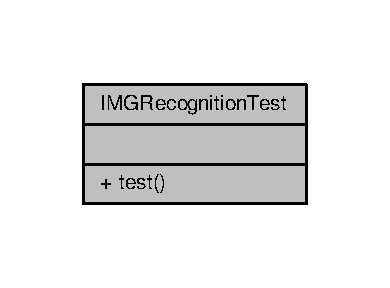
\includegraphics[width=187pt]{classIMGRecognitionTest__coll__graph}
\end{center}
\end{figure}
\subsubsection*{Fonctions membres publiques}
\begin{DoxyCompactItemize}
\item 
void \hyperlink{classIMGRecognitionTest_a5ead096d519c71a800ef6924a74f6bfb}{test} ()
\end{DoxyCompactItemize}


\subsubsection{Documentation des fonctions membres}
\hypertarget{classIMGRecognitionTest_a5ead096d519c71a800ef6924a74f6bfb}{}\index{I\+M\+G\+Recognition\+Test@{I\+M\+G\+Recognition\+Test}!test@{test}}
\index{test@{test}!I\+M\+G\+Recognition\+Test@{I\+M\+G\+Recognition\+Test}}
\paragraph[{test}]{\setlength{\rightskip}{0pt plus 5cm}void I\+M\+G\+Recognition\+Test.\+test (
\begin{DoxyParamCaption}
{}
\end{DoxyParamCaption}
)}\label{classIMGRecognitionTest_a5ead096d519c71a800ef6924a74f6bfb}


La documentation de cette classe a été générée à partir du fichier suivant \+:\begin{DoxyCompactItemize}
\item 
\hyperlink{oldCode_2IMGRecognitionTest_8java}{old\+Code/\+I\+M\+G\+Recognition\+Test.\+java}\end{DoxyCompactItemize}

\hypertarget{classmain_1_1IMGRecognitionTest}{}\subsection{Référence de la classe main.\+I\+M\+G\+Recognition\+Test}
\label{classmain_1_1IMGRecognitionTest}\index{main.\+I\+M\+G\+Recognition\+Test@{main.\+I\+M\+G\+Recognition\+Test}}


Graphe de collaboration de main.\+I\+M\+G\+Recognition\+Test\+:\nopagebreak
\begin{figure}[H]
\begin{center}
\leavevmode
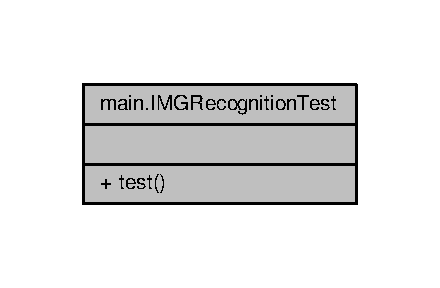
\includegraphics[width=211pt]{classmain_1_1IMGRecognitionTest__coll__graph}
\end{center}
\end{figure}
\subsubsection*{Fonctions membres publiques}
\begin{DoxyCompactItemize}
\item 
void \hyperlink{classmain_1_1IMGRecognitionTest_a4c2f28130c955aade676f31f93a5dae8}{test} ()
\end{DoxyCompactItemize}


\subsubsection{Documentation des fonctions membres}
\hypertarget{classmain_1_1IMGRecognitionTest_a4c2f28130c955aade676f31f93a5dae8}{}\index{main\+::\+I\+M\+G\+Recognition\+Test@{main\+::\+I\+M\+G\+Recognition\+Test}!test@{test}}
\index{test@{test}!main\+::\+I\+M\+G\+Recognition\+Test@{main\+::\+I\+M\+G\+Recognition\+Test}}
\paragraph[{test}]{\setlength{\rightskip}{0pt plus 5cm}void main.\+I\+M\+G\+Recognition\+Test.\+test (
\begin{DoxyParamCaption}
{}
\end{DoxyParamCaption}
)}\label{classmain_1_1IMGRecognitionTest_a4c2f28130c955aade676f31f93a5dae8}


La documentation de cette classe a été générée à partir du fichier suivant \+:\begin{DoxyCompactItemize}
\item 
\hyperlink{main_2IMGRecognitionTest_8java}{main/\+I\+M\+G\+Recognition\+Test.\+java}\end{DoxyCompactItemize}

\hypertarget{classTestSushi_1_1src_1_1Suchi_1_1Maki}{}\subsection{Référence de la classe Test\+Sushi.\+src.\+Suchi.\+Maki}
\label{classTestSushi_1_1src_1_1Suchi_1_1Maki}\index{Test\+Sushi.\+src.\+Suchi.\+Maki@{Test\+Sushi.\+src.\+Suchi.\+Maki}}


Graphe d\textquotesingle{}héritage de Test\+Sushi.\+src.\+Suchi.\+Maki\+:\nopagebreak
\begin{figure}[H]
\begin{center}
\leavevmode
\includegraphics[height=550pt]{classTestSushi_1_1src_1_1Suchi_1_1Maki__inherit__graph}
\end{center}
\end{figure}


Graphe de collaboration de Test\+Sushi.\+src.\+Suchi.\+Maki\+:\nopagebreak
\begin{figure}[H]
\begin{center}
\leavevmode
\includegraphics[height=550pt]{classTestSushi_1_1src_1_1Suchi_1_1Maki__coll__graph}
\end{center}
\end{figure}
\subsubsection*{Fonctions membres publiques}
\begin{DoxyCompactItemize}
\item 
void \hyperlink{classTestSushi_1_1src_1_1Suchi_1_1Maki_a220f1b36947e8e081c0240ad1475ec63}{make} ()  throws A\+W\+T\+Exception, Interrupted\+Exception
\item 
void \hyperlink{classTestSushi_1_1src_1_1Suchi_1_1Maki_af3cd57320dc72b995c05f4a3b1f7ab10}{validate} ()  throws A\+W\+T\+Exception, Interrupted\+Exception 
\item 
void \hyperlink{classTestSushi_1_1src_1_1Suchi_1_1Recette_a2d78a4575d1295e34210e2f77c01f3f3}{use\+Rice} ()  throws A\+W\+T\+Exception, Interrupted\+Exception
\item 
void \hyperlink{classTestSushi_1_1src_1_1Suchi_1_1Recette_a8967a205e78d02ef7c30fd435fbaa0af}{use\+Roe} ()  throws A\+W\+T\+Exception, Interrupted\+Exception
\item 
void \hyperlink{classTestSushi_1_1src_1_1Suchi_1_1Recette_a10bfe3c71750c84144203a7aa2c341ee}{use\+Noori} ()  throws A\+W\+T\+Exception, Interrupted\+Exception
\item 
void \hyperlink{classTestSushi_1_1src_1_1Suchi_1_1Recette_a87cd9338767df0e5db88e6005f1da984}{use\+Salmon} ()  throws A\+W\+T\+Exception, Interrupted\+Exception
\item 
void \hyperlink{classTestSushi_1_1src_1_1Suchi_1_1Recette_ab2c165554830ba84a392765621604d44}{use\+Shrimp} ()  throws A\+W\+T\+Exception, Interrupted\+Exception
\item 
void \hyperlink{classTestSushi_1_1src_1_1Suchi_1_1Recette_a83f9f5fb6bfe2691974a5e35386e7b8a}{check\+Aliment} ()  throws A\+W\+T\+Exception, Interrupted\+Exception
\item 
void \hyperlink{classTestSushi_1_1src_1_1Suchi_1_1Recette_ad94006ea131c2379a14c50eec870b69b}{phone\+Click} ()  throws A\+W\+T\+Exception, Interrupted\+Exception
\item 
void \hyperlink{classTestSushi_1_1src_1_1Suchi_1_1Recette_a33f0912e1212b01ea1b3787bed28f0fe}{validate\+Phone} ()  throws A\+W\+T\+Exception
\item 
void \hyperlink{classTestSushi_1_1src_1_1Suchi_1_1Recette_aa0fc4c335f6ab3f905f63a16902a6379}{buy\+Rice} ()  throws A\+W\+T\+Exception, Interrupted\+Exception
\item 
void \hyperlink{classTestSushi_1_1src_1_1Suchi_1_1Recette_ad874ba9daf68328d6b65b09e6f16003e}{buy\+Roe} ()  throws A\+W\+T\+Exception, Interrupted\+Exception
\item 
void \hyperlink{classTestSushi_1_1src_1_1Suchi_1_1Recette_a5602befaaef8858b75c131e50f7cf91d}{buy\+Noori} ()  throws A\+W\+T\+Exception, Interrupted\+Exception
\item 
void \hyperlink{classTestSushi_1_1src_1_1Suchi_1_1Recette_a64cf6254490e04e9e8031d564a4a0ea3}{buy\+Salmon} ()  throws A\+W\+T\+Exception, Interrupted\+Exception
\item 
void \hyperlink{classTestSushi_1_1src_1_1Suchi_1_1Recette_a0d15202c729b3c6b2bb699de4137d551}{buy\+Shrimp} ()  throws A\+W\+T\+Exception, Interrupted\+Exception
\end{DoxyCompactItemize}
\subsubsection*{Fonctions membres publiques statiques}
\begin{DoxyCompactItemize}
\item 
static void \hyperlink{classTestSushi_1_1src_1_1Suchi_1_1Recette_aef7faa1aea5f8aeb869c612af16e4e62}{reset\+Aliments} ()
\end{DoxyCompactItemize}
\subsubsection*{Attributs protégés}
\begin{DoxyCompactItemize}
\item 
final String \hyperlink{classTestSushi_1_1src_1_1Suchi_1_1Recette_a14892e43d9ed57350effdf3ed1bddb8a}{egggris} = \char`\"{}sprites/egg\+Gris.\+png\char`\"{}
\item 
final String \hyperlink{classTestSushi_1_1src_1_1Suchi_1_1Recette_a774959efa525787a162778df37770b7c}{norigris} = \char`\"{}sprites/nori\+Gris.\+png\char`\"{}
\item 
final String \hyperlink{classTestSushi_1_1src_1_1Suchi_1_1Recette_aea59cc2a5f6bc21ec36690a5bf1eb38c}{saumongris} =\char`\"{}sprites/saumon\+Gris.\+png\char`\"{}
\item 
final String \hyperlink{classTestSushi_1_1src_1_1Suchi_1_1Recette_a616939eea675e05aa6d7ec62fd90f461}{ricegris} = \char`\"{}sprites/rice\+Gris.\+png\char`\"{}
\item 
final String \hyperlink{classTestSushi_1_1src_1_1Suchi_1_1Recette_ac1b1b9b91dba95a9d0df2f6e59f04a59}{shrimp\+Gris} = \char`\"{}sprites/shrimp\+Gris.\+png\char`\"{}
\item 
final Point \hyperlink{classTestSushi_1_1src_1_1Suchi_1_1Recette_a45e48b1a85957813f1a747df04923b08}{phone} = new Point (1030,620)
\item 
final Point \hyperlink{classTestSushi_1_1src_1_1Suchi_1_1Recette_aecc6de3619013f1fb5f506c1e4e9ad7b}{exit\+Phone} = new Point (1050,573)
\item 
final Point \hyperlink{classTestSushi_1_1src_1_1Suchi_1_1Recette_ab502e1d023a0bd3fadfc714e1babc728}{Rice\+C} = new Point (973,503)
\item 
final Point \hyperlink{classTestSushi_1_1src_1_1Suchi_1_1Recette_a890dce3bb5d54a700fa7bebc2496e931}{Rice\+Cbuy} = new Point (976,487)
\item 
final Point \hyperlink{classTestSushi_1_1src_1_1Suchi_1_1Recette_ab7575f64998864f6b053859c18380f58}{Topping} = new Point (978,470)
\item 
final Point \hyperlink{classTestSushi_1_1src_1_1Suchi_1_1Recette_a2f5cec48c186dc52c3d990df66f3a8cf}{fish\+Eggs} = new Point (979,472)
\item 
final Point \hyperlink{classTestSushi_1_1src_1_1Suchi_1_1Recette_a4f3e62b4ab32fcc5d8b6875996f47618}{nori} = new Point (929,469)
\item 
final Point \hyperlink{classTestSushi_1_1src_1_1Suchi_1_1Recette_a9c491e7f09a444817e433e54923e6bca}{validate} = new Point (900,500)
\item 
final Point \hyperlink{classTestSushi_1_1src_1_1Suchi_1_1Recette_a855a7ed217eec3565619156fa6cd4214}{saumon} = new Point (910,560)
\item 
final Point \hyperlink{classTestSushi_1_1src_1_1Suchi_1_1Recette_a69faeadec2c0d475bbd77c3b7eeaada7}{shrimp\+Coord} = new Point (907,386)
\item 
final int \hyperlink{classTestSushi_1_1src_1_1Suchi_1_1Recette_a2c78759553661a7e4b01d4ac1212ec6c}{time} = 150
\item 
final int \hyperlink{classTestSushi_1_1src_1_1Suchi_1_1Recette_a0d95a4a68ee0d423b6815b296f3304b2}{phone\+Time} = 50
\item 
final int \hyperlink{classTestSushi_1_1src_1_1Suchi_1_1Recette_a7db8ec6383e36487bc7ca0490edd0b4a}{time\+Tapis} = 650
\end{DoxyCompactItemize}
\subsubsection*{Attributs protégés statiques}
\begin{DoxyCompactItemize}
\item 
static int \hyperlink{classTestSushi_1_1src_1_1Suchi_1_1Recette_a726a712fe936ef2a96982e00d21c49c0}{salmon} = 5
\item 
static int \hyperlink{classTestSushi_1_1src_1_1Suchi_1_1Recette_a07fa939a0df1b7ff45a9d4aa77498e8e}{shrimp} = 5
\end{DoxyCompactItemize}
\subsubsection*{Fonctions de paquetage}
\begin{DoxyCompactItemize}
\item 
\hyperlink{classTestSushi_1_1src_1_1Suchi_1_1Maki_a94d7a622bf2645cf7a6ac22b723a1fc7}{Maki} ()  throws A\+W\+T\+Exception, Interrupted\+Exception 
\begin{DoxyCompactList}\small\item\em Constructeur. \end{DoxyCompactList}\end{DoxyCompactItemize}
\subsubsection*{Attributs de paquetage}
\begin{DoxyCompactItemize}
\item 
Point \hyperlink{classTestSushi_1_1src_1_1Suchi_1_1Maki_a7a1539e4a06a9c1be0f110e5a667def2}{Noori}
\item 
Point \hyperlink{classTestSushi_1_1src_1_1Suchi_1_1Maki_a4af7a323ffb22f686122932ff113b21a}{Roe}
\end{DoxyCompactItemize}
\subsubsection*{Attributs privés}
\begin{DoxyCompactItemize}
\item 
Point \hyperlink{classTestSushi_1_1src_1_1Suchi_1_1Maki_a45527e39239b51e10268b393645d58f2}{Rice}
\end{DoxyCompactItemize}


\subsubsection{Documentation des constructeurs et destructeur}
\hypertarget{classTestSushi_1_1src_1_1Suchi_1_1Maki_a94d7a622bf2645cf7a6ac22b723a1fc7}{}\index{Test\+Sushi\+::src\+::\+Suchi\+::\+Maki@{Test\+Sushi\+::src\+::\+Suchi\+::\+Maki}!Maki@{Maki}}
\index{Maki@{Maki}!Test\+Sushi\+::src\+::\+Suchi\+::\+Maki@{Test\+Sushi\+::src\+::\+Suchi\+::\+Maki}}
\paragraph[{Maki}]{\setlength{\rightskip}{0pt plus 5cm}Test\+Sushi.\+src.\+Suchi.\+Maki.\+Maki (
\begin{DoxyParamCaption}
{}
\end{DoxyParamCaption}
) throws A\+W\+T\+Exception, Interrupted\+Exception\hspace{0.3cm}{\ttfamily [package]}}\label{classTestSushi_1_1src_1_1Suchi_1_1Maki_a94d7a622bf2645cf7a6ac22b723a1fc7}


Constructeur. 

Va appeller les différentes méthodes pour créer un \hyperlink{classTestSushi_1_1src_1_1Suchi_1_1Maki}{Maki} 
\begin{DoxyExceptions}{Exceptions}
{\em A\+W\+T\+Exception} & \\
\hline
{\em Interrupted\+Exception} & \\
\hline
\end{DoxyExceptions}


\subsubsection{Documentation des fonctions membres}
\hypertarget{classTestSushi_1_1src_1_1Suchi_1_1Recette_a5602befaaef8858b75c131e50f7cf91d}{}\index{Test\+Sushi\+::src\+::\+Suchi\+::\+Maki@{Test\+Sushi\+::src\+::\+Suchi\+::\+Maki}!buy\+Noori@{buy\+Noori}}
\index{buy\+Noori@{buy\+Noori}!Test\+Sushi\+::src\+::\+Suchi\+::\+Maki@{Test\+Sushi\+::src\+::\+Suchi\+::\+Maki}}
\paragraph[{buy\+Noori}]{\setlength{\rightskip}{0pt plus 5cm}void Test\+Sushi.\+src.\+Suchi.\+Recette.\+buy\+Noori (
\begin{DoxyParamCaption}
{}
\end{DoxyParamCaption}
) throws A\+W\+T\+Exception, Interrupted\+Exception\hspace{0.3cm}{\ttfamily [inherited]}}\label{classTestSushi_1_1src_1_1Suchi_1_1Recette_a5602befaaef8858b75c131e50f7cf91d}

\begin{DoxyExceptions}{Exceptions}
{\em A\+W\+T\+Exception} & \\
\hline
{\em Interrupted\+Exception} & \\
\hline
\end{DoxyExceptions}


Référencé par Test\+Sushi.\+src.\+Suchi.\+Recette.\+check\+Aliment().

\hypertarget{classTestSushi_1_1src_1_1Suchi_1_1Recette_aa0fc4c335f6ab3f905f63a16902a6379}{}\index{Test\+Sushi\+::src\+::\+Suchi\+::\+Maki@{Test\+Sushi\+::src\+::\+Suchi\+::\+Maki}!buy\+Rice@{buy\+Rice}}
\index{buy\+Rice@{buy\+Rice}!Test\+Sushi\+::src\+::\+Suchi\+::\+Maki@{Test\+Sushi\+::src\+::\+Suchi\+::\+Maki}}
\paragraph[{buy\+Rice}]{\setlength{\rightskip}{0pt plus 5cm}void Test\+Sushi.\+src.\+Suchi.\+Recette.\+buy\+Rice (
\begin{DoxyParamCaption}
{}
\end{DoxyParamCaption}
) throws A\+W\+T\+Exception, Interrupted\+Exception\hspace{0.3cm}{\ttfamily [inherited]}}\label{classTestSushi_1_1src_1_1Suchi_1_1Recette_aa0fc4c335f6ab3f905f63a16902a6379}

\begin{DoxyExceptions}{Exceptions}
{\em A\+W\+T\+Exception} & \\
\hline
{\em Interrupted\+Exception} & \\
\hline
\end{DoxyExceptions}


Référencé par Test\+Sushi.\+src.\+Suchi.\+Recette.\+check\+Aliment().

\hypertarget{classTestSushi_1_1src_1_1Suchi_1_1Recette_ad874ba9daf68328d6b65b09e6f16003e}{}\index{Test\+Sushi\+::src\+::\+Suchi\+::\+Maki@{Test\+Sushi\+::src\+::\+Suchi\+::\+Maki}!buy\+Roe@{buy\+Roe}}
\index{buy\+Roe@{buy\+Roe}!Test\+Sushi\+::src\+::\+Suchi\+::\+Maki@{Test\+Sushi\+::src\+::\+Suchi\+::\+Maki}}
\paragraph[{buy\+Roe}]{\setlength{\rightskip}{0pt plus 5cm}void Test\+Sushi.\+src.\+Suchi.\+Recette.\+buy\+Roe (
\begin{DoxyParamCaption}
{}
\end{DoxyParamCaption}
) throws A\+W\+T\+Exception, Interrupted\+Exception\hspace{0.3cm}{\ttfamily [inherited]}}\label{classTestSushi_1_1src_1_1Suchi_1_1Recette_ad874ba9daf68328d6b65b09e6f16003e}

\begin{DoxyExceptions}{Exceptions}
{\em A\+W\+T\+Exception} & \\
\hline
{\em Interrupted\+Exception} & \\
\hline
\end{DoxyExceptions}


Référencé par Test\+Sushi.\+src.\+Suchi.\+Recette.\+check\+Aliment().

\hypertarget{classTestSushi_1_1src_1_1Suchi_1_1Recette_a64cf6254490e04e9e8031d564a4a0ea3}{}\index{Test\+Sushi\+::src\+::\+Suchi\+::\+Maki@{Test\+Sushi\+::src\+::\+Suchi\+::\+Maki}!buy\+Salmon@{buy\+Salmon}}
\index{buy\+Salmon@{buy\+Salmon}!Test\+Sushi\+::src\+::\+Suchi\+::\+Maki@{Test\+Sushi\+::src\+::\+Suchi\+::\+Maki}}
\paragraph[{buy\+Salmon}]{\setlength{\rightskip}{0pt plus 5cm}void Test\+Sushi.\+src.\+Suchi.\+Recette.\+buy\+Salmon (
\begin{DoxyParamCaption}
{}
\end{DoxyParamCaption}
) throws A\+W\+T\+Exception, Interrupted\+Exception\hspace{0.3cm}{\ttfamily [inherited]}}\label{classTestSushi_1_1src_1_1Suchi_1_1Recette_a64cf6254490e04e9e8031d564a4a0ea3}

\begin{DoxyExceptions}{Exceptions}
{\em A\+W\+T\+Exception} & \\
\hline
{\em Interrupted\+Exception} & \\
\hline
\end{DoxyExceptions}


Référencé par Test\+Sushi.\+src.\+Suchi.\+Recette.\+check\+Aliment().

\hypertarget{classTestSushi_1_1src_1_1Suchi_1_1Recette_a0d15202c729b3c6b2bb699de4137d551}{}\index{Test\+Sushi\+::src\+::\+Suchi\+::\+Maki@{Test\+Sushi\+::src\+::\+Suchi\+::\+Maki}!buy\+Shrimp@{buy\+Shrimp}}
\index{buy\+Shrimp@{buy\+Shrimp}!Test\+Sushi\+::src\+::\+Suchi\+::\+Maki@{Test\+Sushi\+::src\+::\+Suchi\+::\+Maki}}
\paragraph[{buy\+Shrimp}]{\setlength{\rightskip}{0pt plus 5cm}void Test\+Sushi.\+src.\+Suchi.\+Recette.\+buy\+Shrimp (
\begin{DoxyParamCaption}
{}
\end{DoxyParamCaption}
) throws A\+W\+T\+Exception, Interrupted\+Exception\hspace{0.3cm}{\ttfamily [inherited]}}\label{classTestSushi_1_1src_1_1Suchi_1_1Recette_a0d15202c729b3c6b2bb699de4137d551}

\begin{DoxyExceptions}{Exceptions}
{\em A\+W\+T\+Exception} & \\
\hline
{\em Interrupted\+Exception} & \\
\hline
\end{DoxyExceptions}


Référencé par Test\+Sushi.\+src.\+Suchi.\+Recette.\+check\+Aliment().

\hypertarget{classTestSushi_1_1src_1_1Suchi_1_1Recette_a83f9f5fb6bfe2691974a5e35386e7b8a}{}\index{Test\+Sushi\+::src\+::\+Suchi\+::\+Maki@{Test\+Sushi\+::src\+::\+Suchi\+::\+Maki}!check\+Aliment@{check\+Aliment}}
\index{check\+Aliment@{check\+Aliment}!Test\+Sushi\+::src\+::\+Suchi\+::\+Maki@{Test\+Sushi\+::src\+::\+Suchi\+::\+Maki}}
\paragraph[{check\+Aliment}]{\setlength{\rightskip}{0pt plus 5cm}void Test\+Sushi.\+src.\+Suchi.\+Recette.\+check\+Aliment (
\begin{DoxyParamCaption}
{}
\end{DoxyParamCaption}
) throws A\+W\+T\+Exception, Interrupted\+Exception\hspace{0.3cm}{\ttfamily [inherited]}}\label{classTestSushi_1_1src_1_1Suchi_1_1Recette_a83f9f5fb6bfe2691974a5e35386e7b8a}

\begin{DoxyExceptions}{Exceptions}
{\em A\+W\+T\+Exception} & \\
\hline
{\em Interrupted\+Exception} & \\
\hline
\end{DoxyExceptions}


Référencé par Test\+Sushi.\+src.\+Suchi.\+Recette.\+use\+Noori(), Test\+Sushi.\+src.\+Suchi.\+Recette.\+use\+Rice(), Test\+Sushi.\+src.\+Suchi.\+Recette.\+use\+Roe(), Test\+Sushi.\+src.\+Suchi.\+Recette.\+use\+Salmon(), et Test\+Sushi.\+src.\+Suchi.\+Recette.\+use\+Shrimp().

\hypertarget{classTestSushi_1_1src_1_1Suchi_1_1Maki_a220f1b36947e8e081c0240ad1475ec63}{}\index{Test\+Sushi\+::src\+::\+Suchi\+::\+Maki@{Test\+Sushi\+::src\+::\+Suchi\+::\+Maki}!make@{make}}
\index{make@{make}!Test\+Sushi\+::src\+::\+Suchi\+::\+Maki@{Test\+Sushi\+::src\+::\+Suchi\+::\+Maki}}
\paragraph[{make}]{\setlength{\rightskip}{0pt plus 5cm}void Test\+Sushi.\+src.\+Suchi.\+Maki.\+make (
\begin{DoxyParamCaption}
{}
\end{DoxyParamCaption}
) throws A\+W\+T\+Exception, Interrupted\+Exception}\label{classTestSushi_1_1src_1_1Suchi_1_1Maki_a220f1b36947e8e081c0240ad1475ec63}

\begin{DoxyExceptions}{Exceptions}
{\em A\+W\+T\+Exception} & \\
\hline
{\em Interrupted\+Exception} & \\
\hline
\end{DoxyExceptions}


Référencé par Test\+Sushi.\+src.\+Suchi.\+Maki.\+Maki().

\hypertarget{classTestSushi_1_1src_1_1Suchi_1_1Recette_ad94006ea131c2379a14c50eec870b69b}{}\index{Test\+Sushi\+::src\+::\+Suchi\+::\+Maki@{Test\+Sushi\+::src\+::\+Suchi\+::\+Maki}!phone\+Click@{phone\+Click}}
\index{phone\+Click@{phone\+Click}!Test\+Sushi\+::src\+::\+Suchi\+::\+Maki@{Test\+Sushi\+::src\+::\+Suchi\+::\+Maki}}
\paragraph[{phone\+Click}]{\setlength{\rightskip}{0pt plus 5cm}void Test\+Sushi.\+src.\+Suchi.\+Recette.\+phone\+Click (
\begin{DoxyParamCaption}
{}
\end{DoxyParamCaption}
) throws A\+W\+T\+Exception, Interrupted\+Exception\hspace{0.3cm}{\ttfamily [inherited]}}\label{classTestSushi_1_1src_1_1Suchi_1_1Recette_ad94006ea131c2379a14c50eec870b69b}

\begin{DoxyExceptions}{Exceptions}
{\em A\+W\+T\+Exception} & \\
\hline
{\em Interrupted\+Exception} & \\
\hline
\end{DoxyExceptions}


Référencé par Test\+Sushi.\+src.\+Suchi.\+Recette.\+buy\+Noori(), Test\+Sushi.\+src.\+Suchi.\+Recette.\+buy\+Rice(), Test\+Sushi.\+src.\+Suchi.\+Recette.\+buy\+Roe(), Test\+Sushi.\+src.\+Suchi.\+Recette.\+buy\+Salmon(), et Test\+Sushi.\+src.\+Suchi.\+Recette.\+buy\+Shrimp().

\hypertarget{classTestSushi_1_1src_1_1Suchi_1_1Recette_aef7faa1aea5f8aeb869c612af16e4e62}{}\index{Test\+Sushi\+::src\+::\+Suchi\+::\+Maki@{Test\+Sushi\+::src\+::\+Suchi\+::\+Maki}!reset\+Aliments@{reset\+Aliments}}
\index{reset\+Aliments@{reset\+Aliments}!Test\+Sushi\+::src\+::\+Suchi\+::\+Maki@{Test\+Sushi\+::src\+::\+Suchi\+::\+Maki}}
\paragraph[{reset\+Aliments}]{\setlength{\rightskip}{0pt plus 5cm}static void Test\+Sushi.\+src.\+Suchi.\+Recette.\+reset\+Aliments (
\begin{DoxyParamCaption}
{}
\end{DoxyParamCaption}
)\hspace{0.3cm}{\ttfamily [static]}, {\ttfamily [inherited]}}\label{classTestSushi_1_1src_1_1Suchi_1_1Recette_aef7faa1aea5f8aeb869c612af16e4e62}


Référencé par Test\+Sushi.\+src.\+Suchi.\+Game.\+start\+Level2(), et Test\+Sushi.\+src.\+Suchi.\+Game.\+start\+Level3().

\hypertarget{classTestSushi_1_1src_1_1Suchi_1_1Recette_a10bfe3c71750c84144203a7aa2c341ee}{}\index{Test\+Sushi\+::src\+::\+Suchi\+::\+Maki@{Test\+Sushi\+::src\+::\+Suchi\+::\+Maki}!use\+Noori@{use\+Noori}}
\index{use\+Noori@{use\+Noori}!Test\+Sushi\+::src\+::\+Suchi\+::\+Maki@{Test\+Sushi\+::src\+::\+Suchi\+::\+Maki}}
\paragraph[{use\+Noori}]{\setlength{\rightskip}{0pt plus 5cm}void Test\+Sushi.\+src.\+Suchi.\+Recette.\+use\+Noori (
\begin{DoxyParamCaption}
{}
\end{DoxyParamCaption}
) throws A\+W\+T\+Exception, Interrupted\+Exception\hspace{0.3cm}{\ttfamily [inherited]}}\label{classTestSushi_1_1src_1_1Suchi_1_1Recette_a10bfe3c71750c84144203a7aa2c341ee}

\begin{DoxyExceptions}{Exceptions}
{\em A\+W\+T\+Exception} & \\
\hline
{\em Interrupted\+Exception} & \\
\hline
\end{DoxyExceptions}
\hypertarget{classTestSushi_1_1src_1_1Suchi_1_1Recette_a2d78a4575d1295e34210e2f77c01f3f3}{}\index{Test\+Sushi\+::src\+::\+Suchi\+::\+Maki@{Test\+Sushi\+::src\+::\+Suchi\+::\+Maki}!use\+Rice@{use\+Rice}}
\index{use\+Rice@{use\+Rice}!Test\+Sushi\+::src\+::\+Suchi\+::\+Maki@{Test\+Sushi\+::src\+::\+Suchi\+::\+Maki}}
\paragraph[{use\+Rice}]{\setlength{\rightskip}{0pt plus 5cm}void Test\+Sushi.\+src.\+Suchi.\+Recette.\+use\+Rice (
\begin{DoxyParamCaption}
{}
\end{DoxyParamCaption}
) throws A\+W\+T\+Exception, Interrupted\+Exception\hspace{0.3cm}{\ttfamily [inherited]}}\label{classTestSushi_1_1src_1_1Suchi_1_1Recette_a2d78a4575d1295e34210e2f77c01f3f3}

\begin{DoxyExceptions}{Exceptions}
{\em A\+W\+T\+Exception} & \\
\hline
{\em Interrupted\+Exception} & \\
\hline
\end{DoxyExceptions}
\hypertarget{classTestSushi_1_1src_1_1Suchi_1_1Recette_a8967a205e78d02ef7c30fd435fbaa0af}{}\index{Test\+Sushi\+::src\+::\+Suchi\+::\+Maki@{Test\+Sushi\+::src\+::\+Suchi\+::\+Maki}!use\+Roe@{use\+Roe}}
\index{use\+Roe@{use\+Roe}!Test\+Sushi\+::src\+::\+Suchi\+::\+Maki@{Test\+Sushi\+::src\+::\+Suchi\+::\+Maki}}
\paragraph[{use\+Roe}]{\setlength{\rightskip}{0pt plus 5cm}void Test\+Sushi.\+src.\+Suchi.\+Recette.\+use\+Roe (
\begin{DoxyParamCaption}
{}
\end{DoxyParamCaption}
) throws A\+W\+T\+Exception, Interrupted\+Exception\hspace{0.3cm}{\ttfamily [inherited]}}\label{classTestSushi_1_1src_1_1Suchi_1_1Recette_a8967a205e78d02ef7c30fd435fbaa0af}

\begin{DoxyExceptions}{Exceptions}
{\em A\+W\+T\+Exception} & \\
\hline
{\em Interrupted\+Exception} & \\
\hline
\end{DoxyExceptions}
\hypertarget{classTestSushi_1_1src_1_1Suchi_1_1Recette_a87cd9338767df0e5db88e6005f1da984}{}\index{Test\+Sushi\+::src\+::\+Suchi\+::\+Maki@{Test\+Sushi\+::src\+::\+Suchi\+::\+Maki}!use\+Salmon@{use\+Salmon}}
\index{use\+Salmon@{use\+Salmon}!Test\+Sushi\+::src\+::\+Suchi\+::\+Maki@{Test\+Sushi\+::src\+::\+Suchi\+::\+Maki}}
\paragraph[{use\+Salmon}]{\setlength{\rightskip}{0pt plus 5cm}void Test\+Sushi.\+src.\+Suchi.\+Recette.\+use\+Salmon (
\begin{DoxyParamCaption}
{}
\end{DoxyParamCaption}
) throws A\+W\+T\+Exception, Interrupted\+Exception\hspace{0.3cm}{\ttfamily [inherited]}}\label{classTestSushi_1_1src_1_1Suchi_1_1Recette_a87cd9338767df0e5db88e6005f1da984}

\begin{DoxyExceptions}{Exceptions}
{\em A\+W\+T\+Exception} & \\
\hline
{\em Interrupted\+Exception} & \\
\hline
\end{DoxyExceptions}
\hypertarget{classTestSushi_1_1src_1_1Suchi_1_1Recette_ab2c165554830ba84a392765621604d44}{}\index{Test\+Sushi\+::src\+::\+Suchi\+::\+Maki@{Test\+Sushi\+::src\+::\+Suchi\+::\+Maki}!use\+Shrimp@{use\+Shrimp}}
\index{use\+Shrimp@{use\+Shrimp}!Test\+Sushi\+::src\+::\+Suchi\+::\+Maki@{Test\+Sushi\+::src\+::\+Suchi\+::\+Maki}}
\paragraph[{use\+Shrimp}]{\setlength{\rightskip}{0pt plus 5cm}void Test\+Sushi.\+src.\+Suchi.\+Recette.\+use\+Shrimp (
\begin{DoxyParamCaption}
{}
\end{DoxyParamCaption}
) throws A\+W\+T\+Exception, Interrupted\+Exception\hspace{0.3cm}{\ttfamily [inherited]}}\label{classTestSushi_1_1src_1_1Suchi_1_1Recette_ab2c165554830ba84a392765621604d44}

\begin{DoxyExceptions}{Exceptions}
{\em A\+W\+T\+Exception} & \\
\hline
{\em Interrupted\+Exception} & \\
\hline
\end{DoxyExceptions}
\hypertarget{classTestSushi_1_1src_1_1Suchi_1_1Maki_af3cd57320dc72b995c05f4a3b1f7ab10}{}\index{Test\+Sushi\+::src\+::\+Suchi\+::\+Maki@{Test\+Sushi\+::src\+::\+Suchi\+::\+Maki}!validate@{validate}}
\index{validate@{validate}!Test\+Sushi\+::src\+::\+Suchi\+::\+Maki@{Test\+Sushi\+::src\+::\+Suchi\+::\+Maki}}
\paragraph[{validate}]{\setlength{\rightskip}{0pt plus 5cm}void Test\+Sushi.\+src.\+Suchi.\+Maki.\+validate (
\begin{DoxyParamCaption}
{}
\end{DoxyParamCaption}
) throws A\+W\+T\+Exception, Interrupted\+Exception}\label{classTestSushi_1_1src_1_1Suchi_1_1Maki_af3cd57320dc72b995c05f4a3b1f7ab10}

\begin{DoxyExceptions}{Exceptions}
{\em A\+W\+T\+Exception} & \\
\hline
{\em Interrupted\+Exception} & \\
\hline
\end{DoxyExceptions}


Référencé par Test\+Sushi.\+src.\+Suchi.\+Maki.\+Maki().

\hypertarget{classTestSushi_1_1src_1_1Suchi_1_1Recette_a33f0912e1212b01ea1b3787bed28f0fe}{}\index{Test\+Sushi\+::src\+::\+Suchi\+::\+Maki@{Test\+Sushi\+::src\+::\+Suchi\+::\+Maki}!validate\+Phone@{validate\+Phone}}
\index{validate\+Phone@{validate\+Phone}!Test\+Sushi\+::src\+::\+Suchi\+::\+Maki@{Test\+Sushi\+::src\+::\+Suchi\+::\+Maki}}
\paragraph[{validate\+Phone}]{\setlength{\rightskip}{0pt plus 5cm}void Test\+Sushi.\+src.\+Suchi.\+Recette.\+validate\+Phone (
\begin{DoxyParamCaption}
{}
\end{DoxyParamCaption}
) throws A\+W\+T\+Exception\hspace{0.3cm}{\ttfamily [inherited]}}\label{classTestSushi_1_1src_1_1Suchi_1_1Recette_a33f0912e1212b01ea1b3787bed28f0fe}

\begin{DoxyExceptions}{Exceptions}
{\em A\+W\+T\+Exception} & \\
\hline
\end{DoxyExceptions}


Référencé par Test\+Sushi.\+src.\+Suchi.\+Recette.\+buy\+Noori(), Test\+Sushi.\+src.\+Suchi.\+Recette.\+buy\+Rice(), Test\+Sushi.\+src.\+Suchi.\+Recette.\+buy\+Roe(), Test\+Sushi.\+src.\+Suchi.\+Recette.\+buy\+Salmon(), et Test\+Sushi.\+src.\+Suchi.\+Recette.\+buy\+Shrimp().



\subsubsection{Documentation des données membres}
\hypertarget{classTestSushi_1_1src_1_1Suchi_1_1Recette_a14892e43d9ed57350effdf3ed1bddb8a}{}\index{Test\+Sushi\+::src\+::\+Suchi\+::\+Maki@{Test\+Sushi\+::src\+::\+Suchi\+::\+Maki}!egggris@{egggris}}
\index{egggris@{egggris}!Test\+Sushi\+::src\+::\+Suchi\+::\+Maki@{Test\+Sushi\+::src\+::\+Suchi\+::\+Maki}}
\paragraph[{egggris}]{\setlength{\rightskip}{0pt plus 5cm}final String Test\+Sushi.\+src.\+Suchi.\+Recette.\+egggris = \char`\"{}sprites/egg\+Gris.\+png\char`\"{}\hspace{0.3cm}{\ttfamily [protected]}, {\ttfamily [inherited]}}\label{classTestSushi_1_1src_1_1Suchi_1_1Recette_a14892e43d9ed57350effdf3ed1bddb8a}


Référencé par Test\+Sushi.\+src.\+Suchi.\+Recette.\+buy\+Roe().

\hypertarget{classTestSushi_1_1src_1_1Suchi_1_1Recette_aecc6de3619013f1fb5f506c1e4e9ad7b}{}\index{Test\+Sushi\+::src\+::\+Suchi\+::\+Maki@{Test\+Sushi\+::src\+::\+Suchi\+::\+Maki}!exit\+Phone@{exit\+Phone}}
\index{exit\+Phone@{exit\+Phone}!Test\+Sushi\+::src\+::\+Suchi\+::\+Maki@{Test\+Sushi\+::src\+::\+Suchi\+::\+Maki}}
\paragraph[{exit\+Phone}]{\setlength{\rightskip}{0pt plus 5cm}final Point Test\+Sushi.\+src.\+Suchi.\+Recette.\+exit\+Phone = new Point (1050,573)\hspace{0.3cm}{\ttfamily [protected]}, {\ttfamily [inherited]}}\label{classTestSushi_1_1src_1_1Suchi_1_1Recette_aecc6de3619013f1fb5f506c1e4e9ad7b}
\hypertarget{classTestSushi_1_1src_1_1Suchi_1_1Recette_a2f5cec48c186dc52c3d990df66f3a8cf}{}\index{Test\+Sushi\+::src\+::\+Suchi\+::\+Maki@{Test\+Sushi\+::src\+::\+Suchi\+::\+Maki}!fish\+Eggs@{fish\+Eggs}}
\index{fish\+Eggs@{fish\+Eggs}!Test\+Sushi\+::src\+::\+Suchi\+::\+Maki@{Test\+Sushi\+::src\+::\+Suchi\+::\+Maki}}
\paragraph[{fish\+Eggs}]{\setlength{\rightskip}{0pt plus 5cm}final Point Test\+Sushi.\+src.\+Suchi.\+Recette.\+fish\+Eggs = new Point (979,472)\hspace{0.3cm}{\ttfamily [protected]}, {\ttfamily [inherited]}}\label{classTestSushi_1_1src_1_1Suchi_1_1Recette_a2f5cec48c186dc52c3d990df66f3a8cf}
\hypertarget{classTestSushi_1_1src_1_1Suchi_1_1Maki_a7a1539e4a06a9c1be0f110e5a667def2}{}\index{Test\+Sushi\+::src\+::\+Suchi\+::\+Maki@{Test\+Sushi\+::src\+::\+Suchi\+::\+Maki}!Noori@{Noori}}
\index{Noori@{Noori}!Test\+Sushi\+::src\+::\+Suchi\+::\+Maki@{Test\+Sushi\+::src\+::\+Suchi\+::\+Maki}}
\paragraph[{Noori}]{\setlength{\rightskip}{0pt plus 5cm}Point Test\+Sushi.\+src.\+Suchi.\+Maki.\+Noori\hspace{0.3cm}{\ttfamily [package]}}\label{classTestSushi_1_1src_1_1Suchi_1_1Maki_a7a1539e4a06a9c1be0f110e5a667def2}
\hypertarget{classTestSushi_1_1src_1_1Suchi_1_1Recette_a4f3e62b4ab32fcc5d8b6875996f47618}{}\index{Test\+Sushi\+::src\+::\+Suchi\+::\+Maki@{Test\+Sushi\+::src\+::\+Suchi\+::\+Maki}!nori@{nori}}
\index{nori@{nori}!Test\+Sushi\+::src\+::\+Suchi\+::\+Maki@{Test\+Sushi\+::src\+::\+Suchi\+::\+Maki}}
\paragraph[{nori}]{\setlength{\rightskip}{0pt plus 5cm}final Point Test\+Sushi.\+src.\+Suchi.\+Recette.\+nori = new Point (929,469)\hspace{0.3cm}{\ttfamily [protected]}, {\ttfamily [inherited]}}\label{classTestSushi_1_1src_1_1Suchi_1_1Recette_a4f3e62b4ab32fcc5d8b6875996f47618}
\hypertarget{classTestSushi_1_1src_1_1Suchi_1_1Recette_a774959efa525787a162778df37770b7c}{}\index{Test\+Sushi\+::src\+::\+Suchi\+::\+Maki@{Test\+Sushi\+::src\+::\+Suchi\+::\+Maki}!norigris@{norigris}}
\index{norigris@{norigris}!Test\+Sushi\+::src\+::\+Suchi\+::\+Maki@{Test\+Sushi\+::src\+::\+Suchi\+::\+Maki}}
\paragraph[{norigris}]{\setlength{\rightskip}{0pt plus 5cm}final String Test\+Sushi.\+src.\+Suchi.\+Recette.\+norigris = \char`\"{}sprites/nori\+Gris.\+png\char`\"{}\hspace{0.3cm}{\ttfamily [protected]}, {\ttfamily [inherited]}}\label{classTestSushi_1_1src_1_1Suchi_1_1Recette_a774959efa525787a162778df37770b7c}


Référencé par Test\+Sushi.\+src.\+Suchi.\+Recette.\+buy\+Noori().

\hypertarget{classTestSushi_1_1src_1_1Suchi_1_1Recette_a45e48b1a85957813f1a747df04923b08}{}\index{Test\+Sushi\+::src\+::\+Suchi\+::\+Maki@{Test\+Sushi\+::src\+::\+Suchi\+::\+Maki}!phone@{phone}}
\index{phone@{phone}!Test\+Sushi\+::src\+::\+Suchi\+::\+Maki@{Test\+Sushi\+::src\+::\+Suchi\+::\+Maki}}
\paragraph[{phone}]{\setlength{\rightskip}{0pt plus 5cm}final Point Test\+Sushi.\+src.\+Suchi.\+Recette.\+phone = new Point (1030,620)\hspace{0.3cm}{\ttfamily [protected]}, {\ttfamily [inherited]}}\label{classTestSushi_1_1src_1_1Suchi_1_1Recette_a45e48b1a85957813f1a747df04923b08}
\hypertarget{classTestSushi_1_1src_1_1Suchi_1_1Recette_a0d95a4a68ee0d423b6815b296f3304b2}{}\index{Test\+Sushi\+::src\+::\+Suchi\+::\+Maki@{Test\+Sushi\+::src\+::\+Suchi\+::\+Maki}!phone\+Time@{phone\+Time}}
\index{phone\+Time@{phone\+Time}!Test\+Sushi\+::src\+::\+Suchi\+::\+Maki@{Test\+Sushi\+::src\+::\+Suchi\+::\+Maki}}
\paragraph[{phone\+Time}]{\setlength{\rightskip}{0pt plus 5cm}final int Test\+Sushi.\+src.\+Suchi.\+Recette.\+phone\+Time = 50\hspace{0.3cm}{\ttfamily [protected]}, {\ttfamily [inherited]}}\label{classTestSushi_1_1src_1_1Suchi_1_1Recette_a0d95a4a68ee0d423b6815b296f3304b2}
\hypertarget{classTestSushi_1_1src_1_1Suchi_1_1Maki_a45527e39239b51e10268b393645d58f2}{}\index{Test\+Sushi\+::src\+::\+Suchi\+::\+Maki@{Test\+Sushi\+::src\+::\+Suchi\+::\+Maki}!Rice@{Rice}}
\index{Rice@{Rice}!Test\+Sushi\+::src\+::\+Suchi\+::\+Maki@{Test\+Sushi\+::src\+::\+Suchi\+::\+Maki}}
\paragraph[{Rice}]{\setlength{\rightskip}{0pt plus 5cm}Point Test\+Sushi.\+src.\+Suchi.\+Maki.\+Rice\hspace{0.3cm}{\ttfamily [private]}}\label{classTestSushi_1_1src_1_1Suchi_1_1Maki_a45527e39239b51e10268b393645d58f2}
\hypertarget{classTestSushi_1_1src_1_1Suchi_1_1Recette_ab502e1d023a0bd3fadfc714e1babc728}{}\index{Test\+Sushi\+::src\+::\+Suchi\+::\+Maki@{Test\+Sushi\+::src\+::\+Suchi\+::\+Maki}!Rice\+C@{Rice\+C}}
\index{Rice\+C@{Rice\+C}!Test\+Sushi\+::src\+::\+Suchi\+::\+Maki@{Test\+Sushi\+::src\+::\+Suchi\+::\+Maki}}
\paragraph[{Rice\+C}]{\setlength{\rightskip}{0pt plus 5cm}final Point Test\+Sushi.\+src.\+Suchi.\+Recette.\+Rice\+C = new Point (973,503)\hspace{0.3cm}{\ttfamily [protected]}, {\ttfamily [inherited]}}\label{classTestSushi_1_1src_1_1Suchi_1_1Recette_ab502e1d023a0bd3fadfc714e1babc728}
\hypertarget{classTestSushi_1_1src_1_1Suchi_1_1Recette_a890dce3bb5d54a700fa7bebc2496e931}{}\index{Test\+Sushi\+::src\+::\+Suchi\+::\+Maki@{Test\+Sushi\+::src\+::\+Suchi\+::\+Maki}!Rice\+Cbuy@{Rice\+Cbuy}}
\index{Rice\+Cbuy@{Rice\+Cbuy}!Test\+Sushi\+::src\+::\+Suchi\+::\+Maki@{Test\+Sushi\+::src\+::\+Suchi\+::\+Maki}}
\paragraph[{Rice\+Cbuy}]{\setlength{\rightskip}{0pt plus 5cm}final Point Test\+Sushi.\+src.\+Suchi.\+Recette.\+Rice\+Cbuy = new Point (976,487)\hspace{0.3cm}{\ttfamily [protected]}, {\ttfamily [inherited]}}\label{classTestSushi_1_1src_1_1Suchi_1_1Recette_a890dce3bb5d54a700fa7bebc2496e931}
\hypertarget{classTestSushi_1_1src_1_1Suchi_1_1Recette_a616939eea675e05aa6d7ec62fd90f461}{}\index{Test\+Sushi\+::src\+::\+Suchi\+::\+Maki@{Test\+Sushi\+::src\+::\+Suchi\+::\+Maki}!ricegris@{ricegris}}
\index{ricegris@{ricegris}!Test\+Sushi\+::src\+::\+Suchi\+::\+Maki@{Test\+Sushi\+::src\+::\+Suchi\+::\+Maki}}
\paragraph[{ricegris}]{\setlength{\rightskip}{0pt plus 5cm}final String Test\+Sushi.\+src.\+Suchi.\+Recette.\+ricegris = \char`\"{}sprites/rice\+Gris.\+png\char`\"{}\hspace{0.3cm}{\ttfamily [protected]}, {\ttfamily [inherited]}}\label{classTestSushi_1_1src_1_1Suchi_1_1Recette_a616939eea675e05aa6d7ec62fd90f461}


Référencé par Test\+Sushi.\+src.\+Suchi.\+Recette.\+buy\+Rice().

\hypertarget{classTestSushi_1_1src_1_1Suchi_1_1Maki_a4af7a323ffb22f686122932ff113b21a}{}\index{Test\+Sushi\+::src\+::\+Suchi\+::\+Maki@{Test\+Sushi\+::src\+::\+Suchi\+::\+Maki}!Roe@{Roe}}
\index{Roe@{Roe}!Test\+Sushi\+::src\+::\+Suchi\+::\+Maki@{Test\+Sushi\+::src\+::\+Suchi\+::\+Maki}}
\paragraph[{Roe}]{\setlength{\rightskip}{0pt plus 5cm}Point Test\+Sushi.\+src.\+Suchi.\+Maki.\+Roe\hspace{0.3cm}{\ttfamily [package]}}\label{classTestSushi_1_1src_1_1Suchi_1_1Maki_a4af7a323ffb22f686122932ff113b21a}
\hypertarget{classTestSushi_1_1src_1_1Suchi_1_1Recette_a726a712fe936ef2a96982e00d21c49c0}{}\index{Test\+Sushi\+::src\+::\+Suchi\+::\+Maki@{Test\+Sushi\+::src\+::\+Suchi\+::\+Maki}!salmon@{salmon}}
\index{salmon@{salmon}!Test\+Sushi\+::src\+::\+Suchi\+::\+Maki@{Test\+Sushi\+::src\+::\+Suchi\+::\+Maki}}
\paragraph[{salmon}]{\setlength{\rightskip}{0pt plus 5cm}int Test\+Sushi.\+src.\+Suchi.\+Recette.\+salmon = 5\hspace{0.3cm}{\ttfamily [static]}, {\ttfamily [protected]}, {\ttfamily [inherited]}}\label{classTestSushi_1_1src_1_1Suchi_1_1Recette_a726a712fe936ef2a96982e00d21c49c0}
\hypertarget{classTestSushi_1_1src_1_1Suchi_1_1Recette_a855a7ed217eec3565619156fa6cd4214}{}\index{Test\+Sushi\+::src\+::\+Suchi\+::\+Maki@{Test\+Sushi\+::src\+::\+Suchi\+::\+Maki}!saumon@{saumon}}
\index{saumon@{saumon}!Test\+Sushi\+::src\+::\+Suchi\+::\+Maki@{Test\+Sushi\+::src\+::\+Suchi\+::\+Maki}}
\paragraph[{saumon}]{\setlength{\rightskip}{0pt plus 5cm}final Point Test\+Sushi.\+src.\+Suchi.\+Recette.\+saumon = new Point (910,560)\hspace{0.3cm}{\ttfamily [protected]}, {\ttfamily [inherited]}}\label{classTestSushi_1_1src_1_1Suchi_1_1Recette_a855a7ed217eec3565619156fa6cd4214}
\hypertarget{classTestSushi_1_1src_1_1Suchi_1_1Recette_aea59cc2a5f6bc21ec36690a5bf1eb38c}{}\index{Test\+Sushi\+::src\+::\+Suchi\+::\+Maki@{Test\+Sushi\+::src\+::\+Suchi\+::\+Maki}!saumongris@{saumongris}}
\index{saumongris@{saumongris}!Test\+Sushi\+::src\+::\+Suchi\+::\+Maki@{Test\+Sushi\+::src\+::\+Suchi\+::\+Maki}}
\paragraph[{saumongris}]{\setlength{\rightskip}{0pt plus 5cm}final String Test\+Sushi.\+src.\+Suchi.\+Recette.\+saumongris =\char`\"{}sprites/saumon\+Gris.\+png\char`\"{}\hspace{0.3cm}{\ttfamily [protected]}, {\ttfamily [inherited]}}\label{classTestSushi_1_1src_1_1Suchi_1_1Recette_aea59cc2a5f6bc21ec36690a5bf1eb38c}


Référencé par Test\+Sushi.\+src.\+Suchi.\+Recette.\+buy\+Salmon().

\hypertarget{classTestSushi_1_1src_1_1Suchi_1_1Recette_a07fa939a0df1b7ff45a9d4aa77498e8e}{}\index{Test\+Sushi\+::src\+::\+Suchi\+::\+Maki@{Test\+Sushi\+::src\+::\+Suchi\+::\+Maki}!shrimp@{shrimp}}
\index{shrimp@{shrimp}!Test\+Sushi\+::src\+::\+Suchi\+::\+Maki@{Test\+Sushi\+::src\+::\+Suchi\+::\+Maki}}
\paragraph[{shrimp}]{\setlength{\rightskip}{0pt plus 5cm}int Test\+Sushi.\+src.\+Suchi.\+Recette.\+shrimp = 5\hspace{0.3cm}{\ttfamily [static]}, {\ttfamily [protected]}, {\ttfamily [inherited]}}\label{classTestSushi_1_1src_1_1Suchi_1_1Recette_a07fa939a0df1b7ff45a9d4aa77498e8e}
\hypertarget{classTestSushi_1_1src_1_1Suchi_1_1Recette_a69faeadec2c0d475bbd77c3b7eeaada7}{}\index{Test\+Sushi\+::src\+::\+Suchi\+::\+Maki@{Test\+Sushi\+::src\+::\+Suchi\+::\+Maki}!shrimp\+Coord@{shrimp\+Coord}}
\index{shrimp\+Coord@{shrimp\+Coord}!Test\+Sushi\+::src\+::\+Suchi\+::\+Maki@{Test\+Sushi\+::src\+::\+Suchi\+::\+Maki}}
\paragraph[{shrimp\+Coord}]{\setlength{\rightskip}{0pt plus 5cm}final Point Test\+Sushi.\+src.\+Suchi.\+Recette.\+shrimp\+Coord = new Point (907,386)\hspace{0.3cm}{\ttfamily [protected]}, {\ttfamily [inherited]}}\label{classTestSushi_1_1src_1_1Suchi_1_1Recette_a69faeadec2c0d475bbd77c3b7eeaada7}
\hypertarget{classTestSushi_1_1src_1_1Suchi_1_1Recette_ac1b1b9b91dba95a9d0df2f6e59f04a59}{}\index{Test\+Sushi\+::src\+::\+Suchi\+::\+Maki@{Test\+Sushi\+::src\+::\+Suchi\+::\+Maki}!shrimp\+Gris@{shrimp\+Gris}}
\index{shrimp\+Gris@{shrimp\+Gris}!Test\+Sushi\+::src\+::\+Suchi\+::\+Maki@{Test\+Sushi\+::src\+::\+Suchi\+::\+Maki}}
\paragraph[{shrimp\+Gris}]{\setlength{\rightskip}{0pt plus 5cm}final String Test\+Sushi.\+src.\+Suchi.\+Recette.\+shrimp\+Gris = \char`\"{}sprites/shrimp\+Gris.\+png\char`\"{}\hspace{0.3cm}{\ttfamily [protected]}, {\ttfamily [inherited]}}\label{classTestSushi_1_1src_1_1Suchi_1_1Recette_ac1b1b9b91dba95a9d0df2f6e59f04a59}


Référencé par Test\+Sushi.\+src.\+Suchi.\+Recette.\+buy\+Shrimp().

\hypertarget{classTestSushi_1_1src_1_1Suchi_1_1Recette_a2c78759553661a7e4b01d4ac1212ec6c}{}\index{Test\+Sushi\+::src\+::\+Suchi\+::\+Maki@{Test\+Sushi\+::src\+::\+Suchi\+::\+Maki}!time@{time}}
\index{time@{time}!Test\+Sushi\+::src\+::\+Suchi\+::\+Maki@{Test\+Sushi\+::src\+::\+Suchi\+::\+Maki}}
\paragraph[{time}]{\setlength{\rightskip}{0pt plus 5cm}final int Test\+Sushi.\+src.\+Suchi.\+Recette.\+time = 150\hspace{0.3cm}{\ttfamily [protected]}, {\ttfamily [inherited]}}\label{classTestSushi_1_1src_1_1Suchi_1_1Recette_a2c78759553661a7e4b01d4ac1212ec6c}
\hypertarget{classTestSushi_1_1src_1_1Suchi_1_1Recette_a7db8ec6383e36487bc7ca0490edd0b4a}{}\index{Test\+Sushi\+::src\+::\+Suchi\+::\+Maki@{Test\+Sushi\+::src\+::\+Suchi\+::\+Maki}!time\+Tapis@{time\+Tapis}}
\index{time\+Tapis@{time\+Tapis}!Test\+Sushi\+::src\+::\+Suchi\+::\+Maki@{Test\+Sushi\+::src\+::\+Suchi\+::\+Maki}}
\paragraph[{time\+Tapis}]{\setlength{\rightskip}{0pt plus 5cm}final int Test\+Sushi.\+src.\+Suchi.\+Recette.\+time\+Tapis = 650\hspace{0.3cm}{\ttfamily [protected]}, {\ttfamily [inherited]}}\label{classTestSushi_1_1src_1_1Suchi_1_1Recette_a7db8ec6383e36487bc7ca0490edd0b4a}
\hypertarget{classTestSushi_1_1src_1_1Suchi_1_1Recette_ab7575f64998864f6b053859c18380f58}{}\index{Test\+Sushi\+::src\+::\+Suchi\+::\+Maki@{Test\+Sushi\+::src\+::\+Suchi\+::\+Maki}!Topping@{Topping}}
\index{Topping@{Topping}!Test\+Sushi\+::src\+::\+Suchi\+::\+Maki@{Test\+Sushi\+::src\+::\+Suchi\+::\+Maki}}
\paragraph[{Topping}]{\setlength{\rightskip}{0pt plus 5cm}final Point Test\+Sushi.\+src.\+Suchi.\+Recette.\+Topping = new Point (978,470)\hspace{0.3cm}{\ttfamily [protected]}, {\ttfamily [inherited]}}\label{classTestSushi_1_1src_1_1Suchi_1_1Recette_ab7575f64998864f6b053859c18380f58}
\hypertarget{classTestSushi_1_1src_1_1Suchi_1_1Recette_a9c491e7f09a444817e433e54923e6bca}{}\index{Test\+Sushi\+::src\+::\+Suchi\+::\+Maki@{Test\+Sushi\+::src\+::\+Suchi\+::\+Maki}!validate@{validate}}
\index{validate@{validate}!Test\+Sushi\+::src\+::\+Suchi\+::\+Maki@{Test\+Sushi\+::src\+::\+Suchi\+::\+Maki}}
\paragraph[{validate}]{\setlength{\rightskip}{0pt plus 5cm}final Point Test\+Sushi.\+src.\+Suchi.\+Recette.\+validate = new Point (900,500)\hspace{0.3cm}{\ttfamily [protected]}, {\ttfamily [inherited]}}\label{classTestSushi_1_1src_1_1Suchi_1_1Recette_a9c491e7f09a444817e433e54923e6bca}


La documentation de cette classe a été générée à partir du fichier suivant \+:\begin{DoxyCompactItemize}
\item 
\hyperlink{projet_2TestSushi_2src_2Suchi_2Maki_8java}{projet/\+Test\+Sushi/src/\+Suchi/\+Maki.\+java}\end{DoxyCompactItemize}

\hypertarget{classSuchi_1_1Maki}{}\subsection{Référence de la classe Suchi.\+Maki}
\label{classSuchi_1_1Maki}\index{Suchi.\+Maki@{Suchi.\+Maki}}


Graphe d\textquotesingle{}héritage de Suchi.\+Maki\+:\nopagebreak
\begin{figure}[H]
\begin{center}
\leavevmode
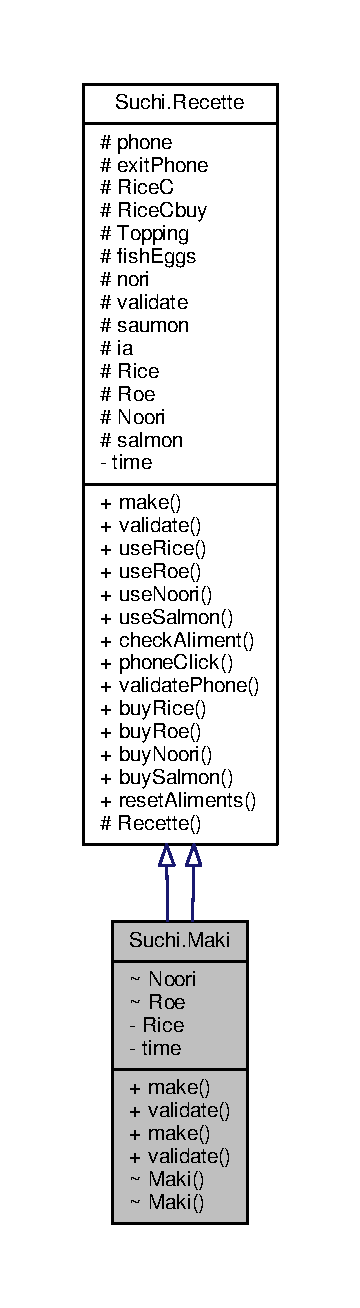
\includegraphics[height=550pt]{classSuchi_1_1Maki__inherit__graph}
\end{center}
\end{figure}


Graphe de collaboration de Suchi.\+Maki\+:\nopagebreak
\begin{figure}[H]
\begin{center}
\leavevmode
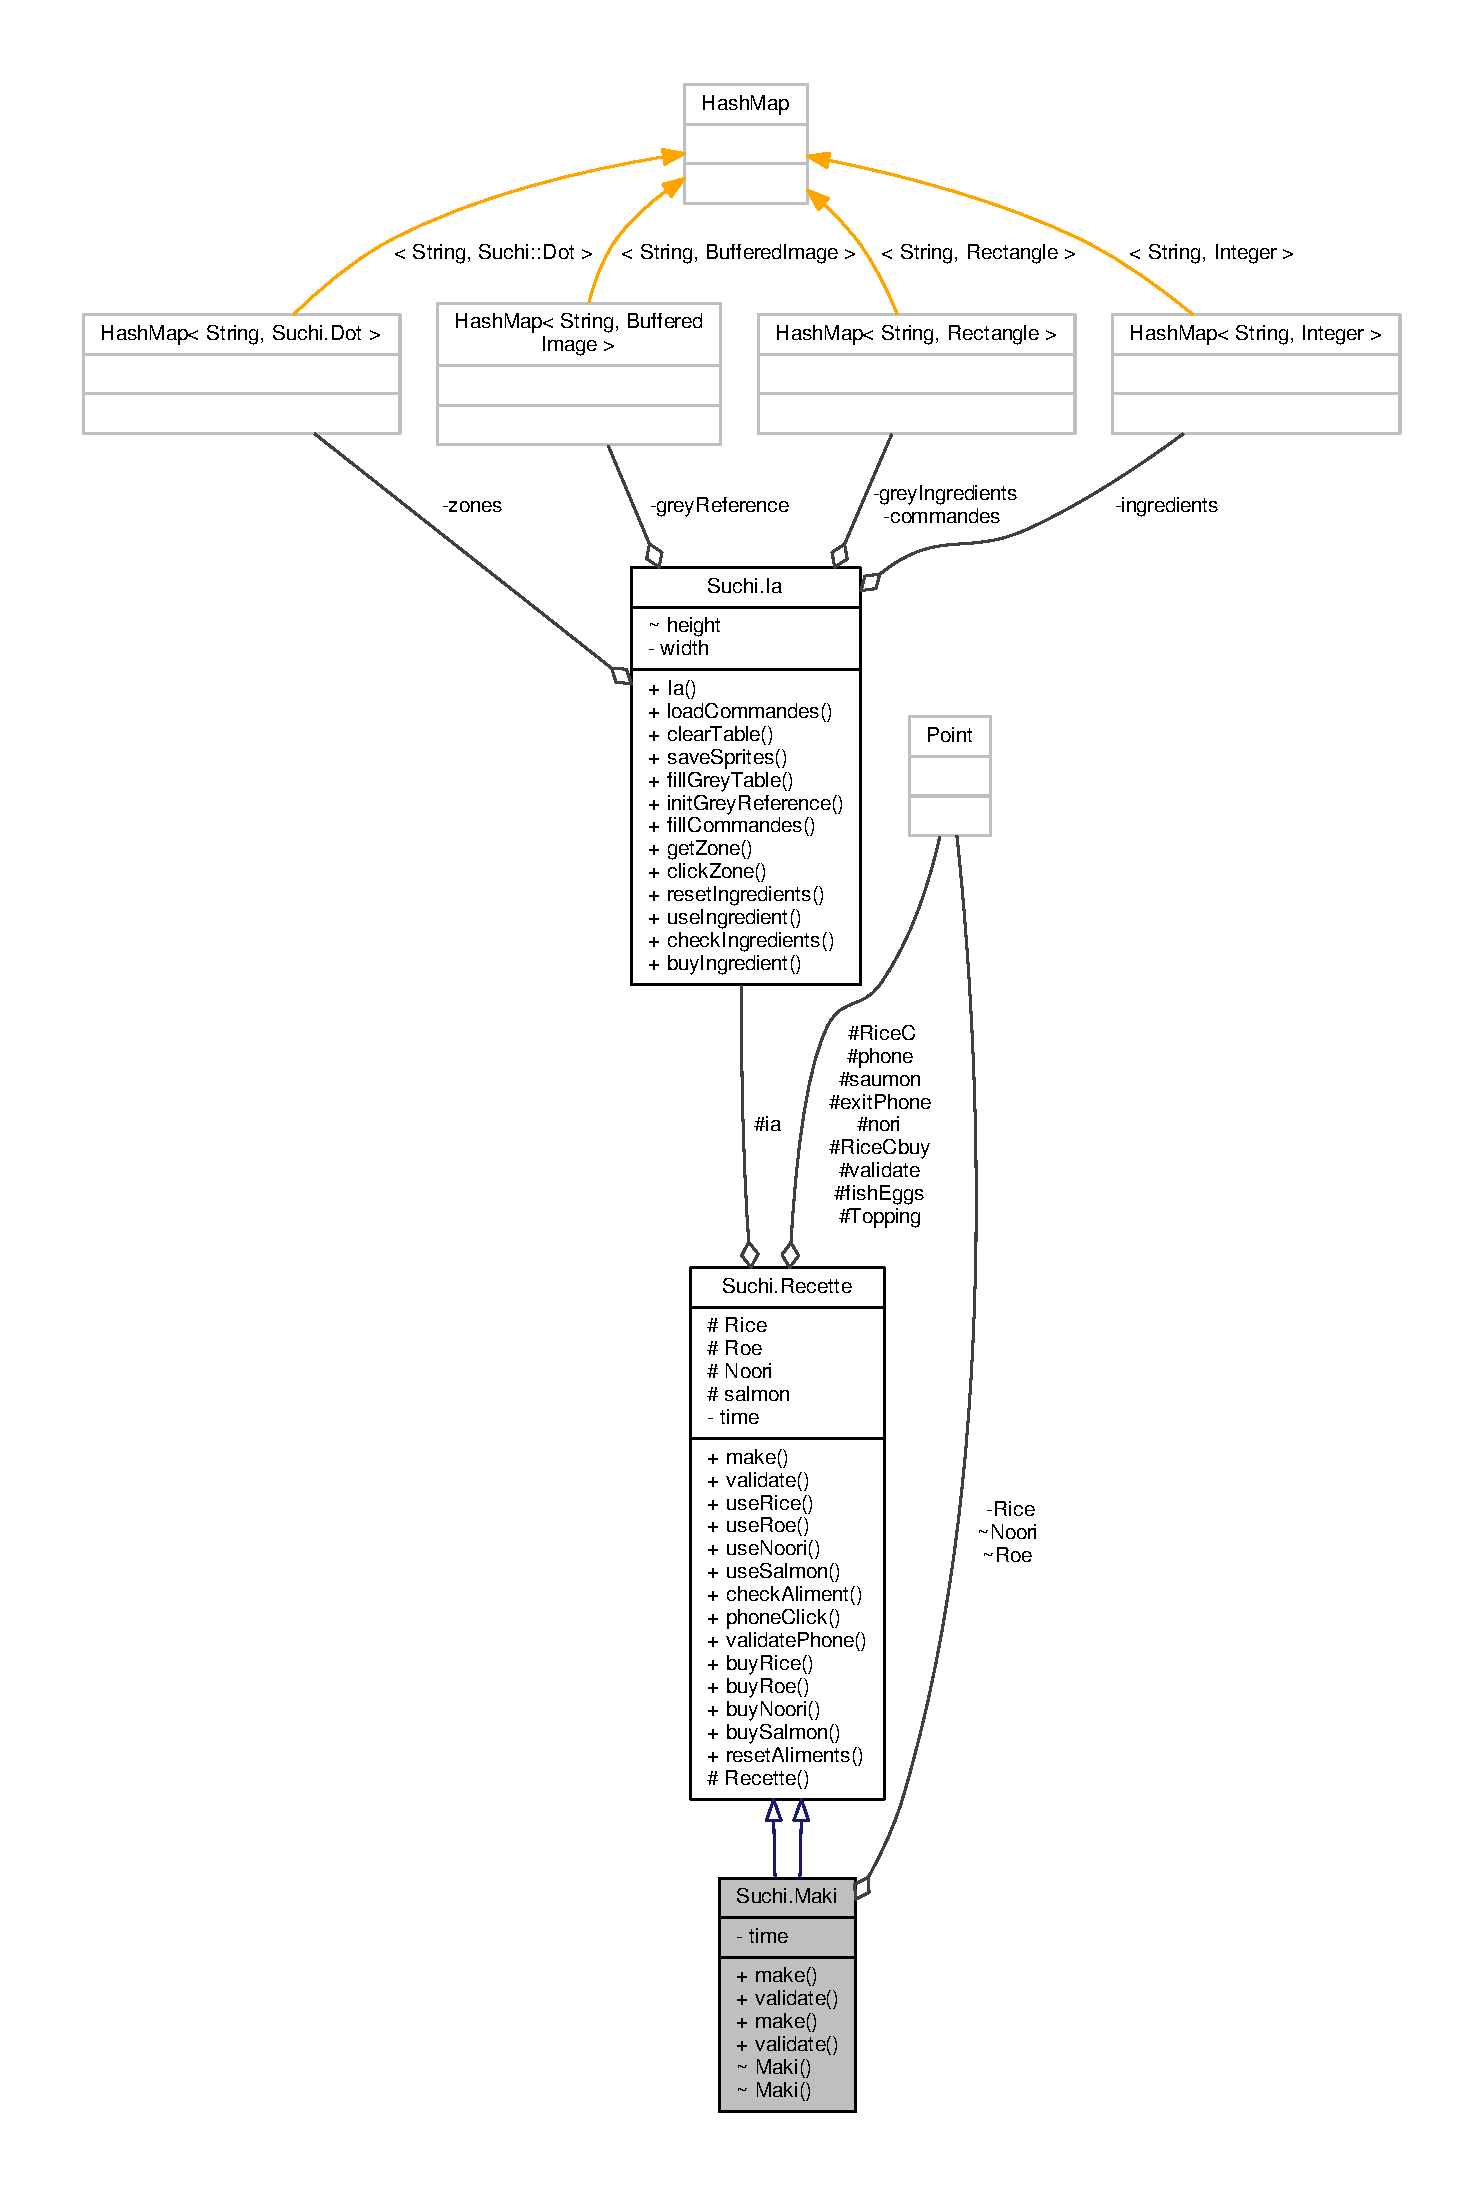
\includegraphics[width=350pt]{classSuchi_1_1Maki__coll__graph}
\end{center}
\end{figure}
\subsubsection*{Fonctions membres publiques}
\begin{DoxyCompactItemize}
\item 
void \hyperlink{classSuchi_1_1Maki_a8133784aaab7730f79ac65efb835b6ee}{make} ()  throws Exception
\item 
void \hyperlink{classSuchi_1_1Maki_adb71be088178ffb1e5fc630da97f55ac}{validate} ()  throws Exception 
\item 
void \hyperlink{classSuchi_1_1Maki_a8133784aaab7730f79ac65efb835b6ee}{make} ()  throws A\+W\+T\+Exception
\item 
void \hyperlink{classSuchi_1_1Maki_adb71be088178ffb1e5fc630da97f55ac}{validate} ()  throws A\+W\+T\+Exception 
\item 
void \hyperlink{classSuchi_1_1Recette_aa5204bd305d5029631ff4b8be9def83e}{use\+Rice} ()  throws A\+W\+T\+Exception, Interrupted\+Exception
\item 
void \hyperlink{classSuchi_1_1Recette_a500a2584148f1f08a1c7cdf7424e9a9c}{use\+Roe} ()  throws A\+W\+T\+Exception, Interrupted\+Exception
\item 
void \hyperlink{classSuchi_1_1Recette_a17d14fe05c28a44768d91e577e9bc511}{use\+Noori} ()  throws A\+W\+T\+Exception, Interrupted\+Exception
\item 
void \hyperlink{classSuchi_1_1Recette_a0fc2aa67439d0822762548c49cb29dec}{use\+Salmon} ()  throws A\+W\+T\+Exception, Interrupted\+Exception
\item 
void \hyperlink{classSuchi_1_1Recette_adc00873c980219a9a3fa7eddeaea3253}{check\+Aliment} ()  throws A\+W\+T\+Exception, Interrupted\+Exception
\item 
void \hyperlink{classSuchi_1_1Recette_a3e4c1e285cd28d0f2f2d364ea637c165}{phone\+Click} ()  throws A\+W\+T\+Exception, Interrupted\+Exception
\item 
void \hyperlink{classSuchi_1_1Recette_aae633102735c0f0a23f0aa84a0366fb3}{validate\+Phone} ()  throws A\+W\+T\+Exception
\item 
void \hyperlink{classSuchi_1_1Recette_a6e0c330317a6f65f2961d35f262362e7}{buy\+Rice} ()  throws A\+W\+T\+Exception, Interrupted\+Exception
\item 
void \hyperlink{classSuchi_1_1Recette_a019d29ed18bfa21dd4bf2ec681761fbf}{buy\+Roe} ()  throws A\+W\+T\+Exception, Interrupted\+Exception
\item 
void \hyperlink{classSuchi_1_1Recette_a31ee8b7bb1aeb396895509a5d5dea094}{buy\+Noori} ()  throws A\+W\+T\+Exception, Interrupted\+Exception
\item 
void \hyperlink{classSuchi_1_1Recette_aef0e38b7827110dbb4fd6a70777cddc1}{buy\+Salmon} ()  throws A\+W\+T\+Exception, Interrupted\+Exception
\end{DoxyCompactItemize}
\subsubsection*{Fonctions membres publiques statiques}
\begin{DoxyCompactItemize}
\item 
static void \hyperlink{classSuchi_1_1Recette_a99446c824f7bffe26c36e8433a4b18b3}{reset\+Aliments} ()
\end{DoxyCompactItemize}
\subsubsection*{Attributs protégés}
\begin{DoxyCompactItemize}
\item 
final Point \hyperlink{classSuchi_1_1Recette_a89465932bd180079526cfc1f8b8af456}{phone} = new Point (1030,620)
\item 
final Point \hyperlink{classSuchi_1_1Recette_ac7ff51ea8fa06174c38c52121b0ef767}{exit\+Phone} = new Point (1050,573)
\item 
final Point \hyperlink{classSuchi_1_1Recette_a36ec8dc3a30b3f1dba74d3aa354f9f11}{Rice\+C} = new Point (973,503)
\item 
final Point \hyperlink{classSuchi_1_1Recette_afc63b1a3fa7d921d606dc0c99d52cdf4}{Rice\+Cbuy} = new Point (976,487)
\item 
final Point \hyperlink{classSuchi_1_1Recette_a4810b2254c050209fba27757066668b3}{Topping} = new Point (978,470)
\item 
final Point \hyperlink{classSuchi_1_1Recette_a9d19fcc0de54e124694592bc35d97a1d}{fish\+Eggs} = new Point (979,472)
\item 
final Point \hyperlink{classSuchi_1_1Recette_ab86193f9fe4491190e232c4e7f93bed5}{nori} = new Point (929,469)
\item 
final Point \hyperlink{classSuchi_1_1Recette_aff16265c9b0b819091af71f64ef84be7}{validate} = new Point (900,500)
\item 
final Point \hyperlink{classSuchi_1_1Recette_a17aeabd21e3d4d55d7caae9a40bfc6a1}{saumon} = new Point (910,560)
\end{DoxyCompactItemize}
\subsubsection*{Attributs protégés statiques}
\begin{DoxyCompactItemize}
\item 
static \hyperlink{classSuchi_1_1Ia}{Ia} \hyperlink{classSuchi_1_1Recette_add9d95ee8955e02592b553c7e4b719a0}{ia}
\item 
static int \hyperlink{classSuchi_1_1Recette_a2e9711072decb1bd2a64a4328e566d73}{salmon} = 5
\end{DoxyCompactItemize}
\subsubsection*{Fonctions de paquetage}
\begin{DoxyCompactItemize}
\item 
\hyperlink{classSuchi_1_1Maki_ac36873f744d39fb04b08d8c1b4ff3abc}{Maki} ()  throws Exception 
\begin{DoxyCompactList}\small\item\em Constructeur. \end{DoxyCompactList}\item 
\hyperlink{classSuchi_1_1Maki_ac36873f744d39fb04b08d8c1b4ff3abc}{Maki} ()  throws A\+W\+T\+Exception, Interrupted\+Exception 
\end{DoxyCompactItemize}
\subsubsection*{Attributs de paquetage}
\begin{DoxyCompactItemize}
\item 
Point \hyperlink{classSuchi_1_1Maki_a045aefe9cf363723101fd82599319ba7}{Noori}
\item 
Point \hyperlink{classSuchi_1_1Maki_a8d8652564efc3073c362f3116c2a1b3c}{Roe}
\end{DoxyCompactItemize}
\subsubsection*{Attributs privés}
\begin{DoxyCompactItemize}
\item 
Point \hyperlink{classSuchi_1_1Maki_a374e7b2bcc840936e61f695ad6960b1b}{Rice}
\item 
int \hyperlink{classSuchi_1_1Maki_a45795f51f5e5e49a3dd2c92428e0652c}{time} = 500
\end{DoxyCompactItemize}


\subsubsection{Documentation des constructeurs et destructeur}
\hypertarget{classSuchi_1_1Maki_ac36873f744d39fb04b08d8c1b4ff3abc}{}\index{Suchi\+::\+Maki@{Suchi\+::\+Maki}!Maki@{Maki}}
\index{Maki@{Maki}!Suchi\+::\+Maki@{Suchi\+::\+Maki}}
\paragraph[{Maki}]{\setlength{\rightskip}{0pt plus 5cm}Suchi.\+Maki.\+Maki (
\begin{DoxyParamCaption}
{}
\end{DoxyParamCaption}
) throws Exception\hspace{0.3cm}{\ttfamily [package]}}\label{classSuchi_1_1Maki_ac36873f744d39fb04b08d8c1b4ff3abc}


Constructeur. 


\begin{DoxyExceptions}{Exceptions}
{\em Exception} & \\
\hline
\end{DoxyExceptions}
\hypertarget{classSuchi_1_1Maki_ac36873f744d39fb04b08d8c1b4ff3abc}{}\index{Suchi\+::\+Maki@{Suchi\+::\+Maki}!Maki@{Maki}}
\index{Maki@{Maki}!Suchi\+::\+Maki@{Suchi\+::\+Maki}}
\paragraph[{Maki}]{\setlength{\rightskip}{0pt plus 5cm}Suchi.\+Maki.\+Maki (
\begin{DoxyParamCaption}
{}
\end{DoxyParamCaption}
) throws A\+W\+T\+Exception, Interrupted\+Exception\hspace{0.3cm}{\ttfamily [package]}}\label{classSuchi_1_1Maki_ac36873f744d39fb04b08d8c1b4ff3abc}


\subsubsection{Documentation des fonctions membres}
\hypertarget{classSuchi_1_1Recette_a31ee8b7bb1aeb396895509a5d5dea094}{}\index{Suchi\+::\+Maki@{Suchi\+::\+Maki}!buy\+Noori@{buy\+Noori}}
\index{buy\+Noori@{buy\+Noori}!Suchi\+::\+Maki@{Suchi\+::\+Maki}}
\paragraph[{buy\+Noori}]{\setlength{\rightskip}{0pt plus 5cm}void Suchi.\+Recette.\+buy\+Noori (
\begin{DoxyParamCaption}
{}
\end{DoxyParamCaption}
) throws A\+W\+T\+Exception, Interrupted\+Exception\hspace{0.3cm}{\ttfamily [inherited]}}\label{classSuchi_1_1Recette_a31ee8b7bb1aeb396895509a5d5dea094}


Référencé par Suchi.\+Recette.\+check\+Aliment().

\hypertarget{classSuchi_1_1Recette_a6e0c330317a6f65f2961d35f262362e7}{}\index{Suchi\+::\+Maki@{Suchi\+::\+Maki}!buy\+Rice@{buy\+Rice}}
\index{buy\+Rice@{buy\+Rice}!Suchi\+::\+Maki@{Suchi\+::\+Maki}}
\paragraph[{buy\+Rice}]{\setlength{\rightskip}{0pt plus 5cm}void Suchi.\+Recette.\+buy\+Rice (
\begin{DoxyParamCaption}
{}
\end{DoxyParamCaption}
) throws A\+W\+T\+Exception, Interrupted\+Exception\hspace{0.3cm}{\ttfamily [inherited]}}\label{classSuchi_1_1Recette_a6e0c330317a6f65f2961d35f262362e7}


Référencé par Suchi.\+Recette.\+check\+Aliment().

\hypertarget{classSuchi_1_1Recette_a019d29ed18bfa21dd4bf2ec681761fbf}{}\index{Suchi\+::\+Maki@{Suchi\+::\+Maki}!buy\+Roe@{buy\+Roe}}
\index{buy\+Roe@{buy\+Roe}!Suchi\+::\+Maki@{Suchi\+::\+Maki}}
\paragraph[{buy\+Roe}]{\setlength{\rightskip}{0pt plus 5cm}void Suchi.\+Recette.\+buy\+Roe (
\begin{DoxyParamCaption}
{}
\end{DoxyParamCaption}
) throws A\+W\+T\+Exception, Interrupted\+Exception\hspace{0.3cm}{\ttfamily [inherited]}}\label{classSuchi_1_1Recette_a019d29ed18bfa21dd4bf2ec681761fbf}


Référencé par Suchi.\+Recette.\+check\+Aliment().

\hypertarget{classSuchi_1_1Recette_aef0e38b7827110dbb4fd6a70777cddc1}{}\index{Suchi\+::\+Maki@{Suchi\+::\+Maki}!buy\+Salmon@{buy\+Salmon}}
\index{buy\+Salmon@{buy\+Salmon}!Suchi\+::\+Maki@{Suchi\+::\+Maki}}
\paragraph[{buy\+Salmon}]{\setlength{\rightskip}{0pt plus 5cm}void Suchi.\+Recette.\+buy\+Salmon (
\begin{DoxyParamCaption}
{}
\end{DoxyParamCaption}
) throws A\+W\+T\+Exception, Interrupted\+Exception\hspace{0.3cm}{\ttfamily [inherited]}}\label{classSuchi_1_1Recette_aef0e38b7827110dbb4fd6a70777cddc1}


Référencé par Suchi.\+Recette.\+check\+Aliment().

\hypertarget{classSuchi_1_1Recette_adc00873c980219a9a3fa7eddeaea3253}{}\index{Suchi\+::\+Maki@{Suchi\+::\+Maki}!check\+Aliment@{check\+Aliment}}
\index{check\+Aliment@{check\+Aliment}!Suchi\+::\+Maki@{Suchi\+::\+Maki}}
\paragraph[{check\+Aliment}]{\setlength{\rightskip}{0pt plus 5cm}void Suchi.\+Recette.\+check\+Aliment (
\begin{DoxyParamCaption}
{}
\end{DoxyParamCaption}
) throws A\+W\+T\+Exception, Interrupted\+Exception\hspace{0.3cm}{\ttfamily [inherited]}}\label{classSuchi_1_1Recette_adc00873c980219a9a3fa7eddeaea3253}


Référencé par Suchi.\+Recette.\+use\+Noori(), Suchi.\+Recette.\+use\+Rice(), Suchi.\+Recette.\+use\+Roe(), et Suchi.\+Recette.\+use\+Salmon().

\hypertarget{classSuchi_1_1Maki_a8133784aaab7730f79ac65efb835b6ee}{}\index{Suchi\+::\+Maki@{Suchi\+::\+Maki}!make@{make}}
\index{make@{make}!Suchi\+::\+Maki@{Suchi\+::\+Maki}}
\paragraph[{make}]{\setlength{\rightskip}{0pt plus 5cm}void Suchi.\+Maki.\+make (
\begin{DoxyParamCaption}
{}
\end{DoxyParamCaption}
) throws Exception}\label{classSuchi_1_1Maki_a8133784aaab7730f79ac65efb835b6ee}


Référencé par Suchi.\+Maki.\+Maki().

\hypertarget{classSuchi_1_1Maki_a8133784aaab7730f79ac65efb835b6ee}{}\index{Suchi\+::\+Maki@{Suchi\+::\+Maki}!make@{make}}
\index{make@{make}!Suchi\+::\+Maki@{Suchi\+::\+Maki}}
\paragraph[{make}]{\setlength{\rightskip}{0pt plus 5cm}void Suchi.\+Maki.\+make (
\begin{DoxyParamCaption}
{}
\end{DoxyParamCaption}
) throws A\+W\+T\+Exception}\label{classSuchi_1_1Maki_a8133784aaab7730f79ac65efb835b6ee}
\hypertarget{classSuchi_1_1Recette_a3e4c1e285cd28d0f2f2d364ea637c165}{}\index{Suchi\+::\+Maki@{Suchi\+::\+Maki}!phone\+Click@{phone\+Click}}
\index{phone\+Click@{phone\+Click}!Suchi\+::\+Maki@{Suchi\+::\+Maki}}
\paragraph[{phone\+Click}]{\setlength{\rightskip}{0pt plus 5cm}void Suchi.\+Recette.\+phone\+Click (
\begin{DoxyParamCaption}
{}
\end{DoxyParamCaption}
) throws A\+W\+T\+Exception, Interrupted\+Exception\hspace{0.3cm}{\ttfamily [inherited]}}\label{classSuchi_1_1Recette_a3e4c1e285cd28d0f2f2d364ea637c165}


Référencé par Suchi.\+Recette.\+buy\+Noori(), Suchi.\+Recette.\+buy\+Rice(), Suchi.\+Recette.\+buy\+Roe(), et Suchi.\+Recette.\+buy\+Salmon().

\hypertarget{classSuchi_1_1Recette_a99446c824f7bffe26c36e8433a4b18b3}{}\index{Suchi\+::\+Maki@{Suchi\+::\+Maki}!reset\+Aliments@{reset\+Aliments}}
\index{reset\+Aliments@{reset\+Aliments}!Suchi\+::\+Maki@{Suchi\+::\+Maki}}
\paragraph[{reset\+Aliments}]{\setlength{\rightskip}{0pt plus 5cm}static void Suchi.\+Recette.\+reset\+Aliments (
\begin{DoxyParamCaption}
{}
\end{DoxyParamCaption}
)\hspace{0.3cm}{\ttfamily [static]}, {\ttfamily [inherited]}}\label{classSuchi_1_1Recette_a99446c824f7bffe26c36e8433a4b18b3}


Référencé par Suchi.\+Game.\+main().

\hypertarget{classSuchi_1_1Recette_a17d14fe05c28a44768d91e577e9bc511}{}\index{Suchi\+::\+Maki@{Suchi\+::\+Maki}!use\+Noori@{use\+Noori}}
\index{use\+Noori@{use\+Noori}!Suchi\+::\+Maki@{Suchi\+::\+Maki}}
\paragraph[{use\+Noori}]{\setlength{\rightskip}{0pt plus 5cm}void Suchi.\+Recette.\+use\+Noori (
\begin{DoxyParamCaption}
{}
\end{DoxyParamCaption}
) throws A\+W\+T\+Exception, Interrupted\+Exception\hspace{0.3cm}{\ttfamily [inherited]}}\label{classSuchi_1_1Recette_a17d14fe05c28a44768d91e577e9bc511}
\hypertarget{classSuchi_1_1Recette_aa5204bd305d5029631ff4b8be9def83e}{}\index{Suchi\+::\+Maki@{Suchi\+::\+Maki}!use\+Rice@{use\+Rice}}
\index{use\+Rice@{use\+Rice}!Suchi\+::\+Maki@{Suchi\+::\+Maki}}
\paragraph[{use\+Rice}]{\setlength{\rightskip}{0pt plus 5cm}void Suchi.\+Recette.\+use\+Rice (
\begin{DoxyParamCaption}
{}
\end{DoxyParamCaption}
) throws A\+W\+T\+Exception, Interrupted\+Exception\hspace{0.3cm}{\ttfamily [inherited]}}\label{classSuchi_1_1Recette_aa5204bd305d5029631ff4b8be9def83e}
\hypertarget{classSuchi_1_1Recette_a500a2584148f1f08a1c7cdf7424e9a9c}{}\index{Suchi\+::\+Maki@{Suchi\+::\+Maki}!use\+Roe@{use\+Roe}}
\index{use\+Roe@{use\+Roe}!Suchi\+::\+Maki@{Suchi\+::\+Maki}}
\paragraph[{use\+Roe}]{\setlength{\rightskip}{0pt plus 5cm}void Suchi.\+Recette.\+use\+Roe (
\begin{DoxyParamCaption}
{}
\end{DoxyParamCaption}
) throws A\+W\+T\+Exception, Interrupted\+Exception\hspace{0.3cm}{\ttfamily [inherited]}}\label{classSuchi_1_1Recette_a500a2584148f1f08a1c7cdf7424e9a9c}
\hypertarget{classSuchi_1_1Recette_a0fc2aa67439d0822762548c49cb29dec}{}\index{Suchi\+::\+Maki@{Suchi\+::\+Maki}!use\+Salmon@{use\+Salmon}}
\index{use\+Salmon@{use\+Salmon}!Suchi\+::\+Maki@{Suchi\+::\+Maki}}
\paragraph[{use\+Salmon}]{\setlength{\rightskip}{0pt plus 5cm}void Suchi.\+Recette.\+use\+Salmon (
\begin{DoxyParamCaption}
{}
\end{DoxyParamCaption}
) throws A\+W\+T\+Exception, Interrupted\+Exception\hspace{0.3cm}{\ttfamily [inherited]}}\label{classSuchi_1_1Recette_a0fc2aa67439d0822762548c49cb29dec}
\hypertarget{classSuchi_1_1Maki_adb71be088178ffb1e5fc630da97f55ac}{}\index{Suchi\+::\+Maki@{Suchi\+::\+Maki}!validate@{validate}}
\index{validate@{validate}!Suchi\+::\+Maki@{Suchi\+::\+Maki}}
\paragraph[{validate}]{\setlength{\rightskip}{0pt plus 5cm}void Suchi.\+Maki.\+validate (
\begin{DoxyParamCaption}
{}
\end{DoxyParamCaption}
) throws Exception}\label{classSuchi_1_1Maki_adb71be088178ffb1e5fc630da97f55ac}


Référencé par Suchi.\+Maki.\+Maki().

\hypertarget{classSuchi_1_1Maki_adb71be088178ffb1e5fc630da97f55ac}{}\index{Suchi\+::\+Maki@{Suchi\+::\+Maki}!validate@{validate}}
\index{validate@{validate}!Suchi\+::\+Maki@{Suchi\+::\+Maki}}
\paragraph[{validate}]{\setlength{\rightskip}{0pt plus 5cm}void Suchi.\+Maki.\+validate (
\begin{DoxyParamCaption}
{}
\end{DoxyParamCaption}
) throws A\+W\+T\+Exception}\label{classSuchi_1_1Maki_adb71be088178ffb1e5fc630da97f55ac}
\hypertarget{classSuchi_1_1Recette_aae633102735c0f0a23f0aa84a0366fb3}{}\index{Suchi\+::\+Maki@{Suchi\+::\+Maki}!validate\+Phone@{validate\+Phone}}
\index{validate\+Phone@{validate\+Phone}!Suchi\+::\+Maki@{Suchi\+::\+Maki}}
\paragraph[{validate\+Phone}]{\setlength{\rightskip}{0pt plus 5cm}void Suchi.\+Recette.\+validate\+Phone (
\begin{DoxyParamCaption}
{}
\end{DoxyParamCaption}
) throws A\+W\+T\+Exception\hspace{0.3cm}{\ttfamily [inherited]}}\label{classSuchi_1_1Recette_aae633102735c0f0a23f0aa84a0366fb3}


Référencé par Suchi.\+Recette.\+buy\+Noori(), Suchi.\+Recette.\+buy\+Rice(), Suchi.\+Recette.\+buy\+Roe(), et Suchi.\+Recette.\+buy\+Salmon().



\subsubsection{Documentation des données membres}
\hypertarget{classSuchi_1_1Recette_ac7ff51ea8fa06174c38c52121b0ef767}{}\index{Suchi\+::\+Maki@{Suchi\+::\+Maki}!exit\+Phone@{exit\+Phone}}
\index{exit\+Phone@{exit\+Phone}!Suchi\+::\+Maki@{Suchi\+::\+Maki}}
\paragraph[{exit\+Phone}]{\setlength{\rightskip}{0pt plus 5cm}final Point Suchi.\+Recette.\+exit\+Phone = new Point (1050,573)\hspace{0.3cm}{\ttfamily [protected]}, {\ttfamily [inherited]}}\label{classSuchi_1_1Recette_ac7ff51ea8fa06174c38c52121b0ef767}
\hypertarget{classSuchi_1_1Recette_a9d19fcc0de54e124694592bc35d97a1d}{}\index{Suchi\+::\+Maki@{Suchi\+::\+Maki}!fish\+Eggs@{fish\+Eggs}}
\index{fish\+Eggs@{fish\+Eggs}!Suchi\+::\+Maki@{Suchi\+::\+Maki}}
\paragraph[{fish\+Eggs}]{\setlength{\rightskip}{0pt plus 5cm}final Point Suchi.\+Recette.\+fish\+Eggs = new Point (979,472)\hspace{0.3cm}{\ttfamily [protected]}, {\ttfamily [inherited]}}\label{classSuchi_1_1Recette_a9d19fcc0de54e124694592bc35d97a1d}
\hypertarget{classSuchi_1_1Recette_add9d95ee8955e02592b553c7e4b719a0}{}\index{Suchi\+::\+Maki@{Suchi\+::\+Maki}!ia@{ia}}
\index{ia@{ia}!Suchi\+::\+Maki@{Suchi\+::\+Maki}}
\paragraph[{ia}]{\setlength{\rightskip}{0pt plus 5cm}{\bf Ia} Suchi.\+Recette.\+ia\hspace{0.3cm}{\ttfamily [static]}, {\ttfamily [protected]}, {\ttfamily [inherited]}}\label{classSuchi_1_1Recette_add9d95ee8955e02592b553c7e4b719a0}


Référencé par Suchi.\+Salmon.\+make(), Suchi.\+California.\+make(), Suchi.\+Maki.\+make(), Suchi.\+Onigiri.\+make(), Suchi.\+Shrimp\+Sh.\+make(), Suchi.\+Onigiri.\+validate(), Suchi.\+Salmon.\+validate(), Suchi.\+California.\+validate(), Suchi.\+Maki.\+validate(), et Suchi.\+Shrimp\+Sh.\+validate().

\hypertarget{classSuchi_1_1Maki_a045aefe9cf363723101fd82599319ba7}{}\index{Suchi\+::\+Maki@{Suchi\+::\+Maki}!Noori@{Noori}}
\index{Noori@{Noori}!Suchi\+::\+Maki@{Suchi\+::\+Maki}}
\paragraph[{Noori}]{\setlength{\rightskip}{0pt plus 5cm}Point Suchi.\+Maki.\+Noori\hspace{0.3cm}{\ttfamily [package]}}\label{classSuchi_1_1Maki_a045aefe9cf363723101fd82599319ba7}
\hypertarget{classSuchi_1_1Recette_ab86193f9fe4491190e232c4e7f93bed5}{}\index{Suchi\+::\+Maki@{Suchi\+::\+Maki}!nori@{nori}}
\index{nori@{nori}!Suchi\+::\+Maki@{Suchi\+::\+Maki}}
\paragraph[{nori}]{\setlength{\rightskip}{0pt plus 5cm}final Point Suchi.\+Recette.\+nori = new Point (929,469)\hspace{0.3cm}{\ttfamily [protected]}, {\ttfamily [inherited]}}\label{classSuchi_1_1Recette_ab86193f9fe4491190e232c4e7f93bed5}
\hypertarget{classSuchi_1_1Recette_a89465932bd180079526cfc1f8b8af456}{}\index{Suchi\+::\+Maki@{Suchi\+::\+Maki}!phone@{phone}}
\index{phone@{phone}!Suchi\+::\+Maki@{Suchi\+::\+Maki}}
\paragraph[{phone}]{\setlength{\rightskip}{0pt plus 5cm}final Point Suchi.\+Recette.\+phone = new Point (1030,620)\hspace{0.3cm}{\ttfamily [protected]}, {\ttfamily [inherited]}}\label{classSuchi_1_1Recette_a89465932bd180079526cfc1f8b8af456}
\hypertarget{classSuchi_1_1Maki_a374e7b2bcc840936e61f695ad6960b1b}{}\index{Suchi\+::\+Maki@{Suchi\+::\+Maki}!Rice@{Rice}}
\index{Rice@{Rice}!Suchi\+::\+Maki@{Suchi\+::\+Maki}}
\paragraph[{Rice}]{\setlength{\rightskip}{0pt plus 5cm}Point Suchi.\+Maki.\+Rice\hspace{0.3cm}{\ttfamily [private]}}\label{classSuchi_1_1Maki_a374e7b2bcc840936e61f695ad6960b1b}
\hypertarget{classSuchi_1_1Recette_a36ec8dc3a30b3f1dba74d3aa354f9f11}{}\index{Suchi\+::\+Maki@{Suchi\+::\+Maki}!Rice\+C@{Rice\+C}}
\index{Rice\+C@{Rice\+C}!Suchi\+::\+Maki@{Suchi\+::\+Maki}}
\paragraph[{Rice\+C}]{\setlength{\rightskip}{0pt plus 5cm}final Point Suchi.\+Recette.\+Rice\+C = new Point (973,503)\hspace{0.3cm}{\ttfamily [protected]}, {\ttfamily [inherited]}}\label{classSuchi_1_1Recette_a36ec8dc3a30b3f1dba74d3aa354f9f11}
\hypertarget{classSuchi_1_1Recette_afc63b1a3fa7d921d606dc0c99d52cdf4}{}\index{Suchi\+::\+Maki@{Suchi\+::\+Maki}!Rice\+Cbuy@{Rice\+Cbuy}}
\index{Rice\+Cbuy@{Rice\+Cbuy}!Suchi\+::\+Maki@{Suchi\+::\+Maki}}
\paragraph[{Rice\+Cbuy}]{\setlength{\rightskip}{0pt plus 5cm}final Point Suchi.\+Recette.\+Rice\+Cbuy = new Point (976,487)\hspace{0.3cm}{\ttfamily [protected]}, {\ttfamily [inherited]}}\label{classSuchi_1_1Recette_afc63b1a3fa7d921d606dc0c99d52cdf4}
\hypertarget{classSuchi_1_1Maki_a8d8652564efc3073c362f3116c2a1b3c}{}\index{Suchi\+::\+Maki@{Suchi\+::\+Maki}!Roe@{Roe}}
\index{Roe@{Roe}!Suchi\+::\+Maki@{Suchi\+::\+Maki}}
\paragraph[{Roe}]{\setlength{\rightskip}{0pt plus 5cm}Point Suchi.\+Maki.\+Roe\hspace{0.3cm}{\ttfamily [package]}}\label{classSuchi_1_1Maki_a8d8652564efc3073c362f3116c2a1b3c}
\hypertarget{classSuchi_1_1Recette_a2e9711072decb1bd2a64a4328e566d73}{}\index{Suchi\+::\+Maki@{Suchi\+::\+Maki}!salmon@{salmon}}
\index{salmon@{salmon}!Suchi\+::\+Maki@{Suchi\+::\+Maki}}
\paragraph[{salmon}]{\setlength{\rightskip}{0pt plus 5cm}int Suchi.\+Recette.\+salmon = 5\hspace{0.3cm}{\ttfamily [static]}, {\ttfamily [protected]}, {\ttfamily [inherited]}}\label{classSuchi_1_1Recette_a2e9711072decb1bd2a64a4328e566d73}
\hypertarget{classSuchi_1_1Recette_a17aeabd21e3d4d55d7caae9a40bfc6a1}{}\index{Suchi\+::\+Maki@{Suchi\+::\+Maki}!saumon@{saumon}}
\index{saumon@{saumon}!Suchi\+::\+Maki@{Suchi\+::\+Maki}}
\paragraph[{saumon}]{\setlength{\rightskip}{0pt plus 5cm}final Point Suchi.\+Recette.\+saumon = new Point (910,560)\hspace{0.3cm}{\ttfamily [protected]}, {\ttfamily [inherited]}}\label{classSuchi_1_1Recette_a17aeabd21e3d4d55d7caae9a40bfc6a1}
\hypertarget{classSuchi_1_1Maki_a45795f51f5e5e49a3dd2c92428e0652c}{}\index{Suchi\+::\+Maki@{Suchi\+::\+Maki}!time@{time}}
\index{time@{time}!Suchi\+::\+Maki@{Suchi\+::\+Maki}}
\paragraph[{time}]{\setlength{\rightskip}{0pt plus 5cm}int Suchi.\+Maki.\+time = 500\hspace{0.3cm}{\ttfamily [private]}}\label{classSuchi_1_1Maki_a45795f51f5e5e49a3dd2c92428e0652c}
\hypertarget{classSuchi_1_1Recette_a4810b2254c050209fba27757066668b3}{}\index{Suchi\+::\+Maki@{Suchi\+::\+Maki}!Topping@{Topping}}
\index{Topping@{Topping}!Suchi\+::\+Maki@{Suchi\+::\+Maki}}
\paragraph[{Topping}]{\setlength{\rightskip}{0pt plus 5cm}final Point Suchi.\+Recette.\+Topping = new Point (978,470)\hspace{0.3cm}{\ttfamily [protected]}, {\ttfamily [inherited]}}\label{classSuchi_1_1Recette_a4810b2254c050209fba27757066668b3}
\hypertarget{classSuchi_1_1Recette_aff16265c9b0b819091af71f64ef84be7}{}\index{Suchi\+::\+Maki@{Suchi\+::\+Maki}!validate@{validate}}
\index{validate@{validate}!Suchi\+::\+Maki@{Suchi\+::\+Maki}}
\paragraph[{validate}]{\setlength{\rightskip}{0pt plus 5cm}final Point Suchi.\+Recette.\+validate = new Point (900,500)\hspace{0.3cm}{\ttfamily [protected]}, {\ttfamily [inherited]}}\label{classSuchi_1_1Recette_aff16265c9b0b819091af71f64ef84be7}


La documentation de cette classe a été générée à partir du fichier suivant \+:\begin{DoxyCompactItemize}
\item 
\hyperlink{BotSofRetapage_2src_2Suchi_2Maki_8java}{Bot\+Sof\+Retapage/src/\+Suchi/\+Maki.\+java}\end{DoxyCompactItemize}

\hypertarget{classManager}{}\subsection{Référence de la classe Manager}
\label{classManager}\index{Manager@{Manager}}


Graphe de collaboration de Manager\+:\nopagebreak
\begin{figure}[H]
\begin{center}
\leavevmode
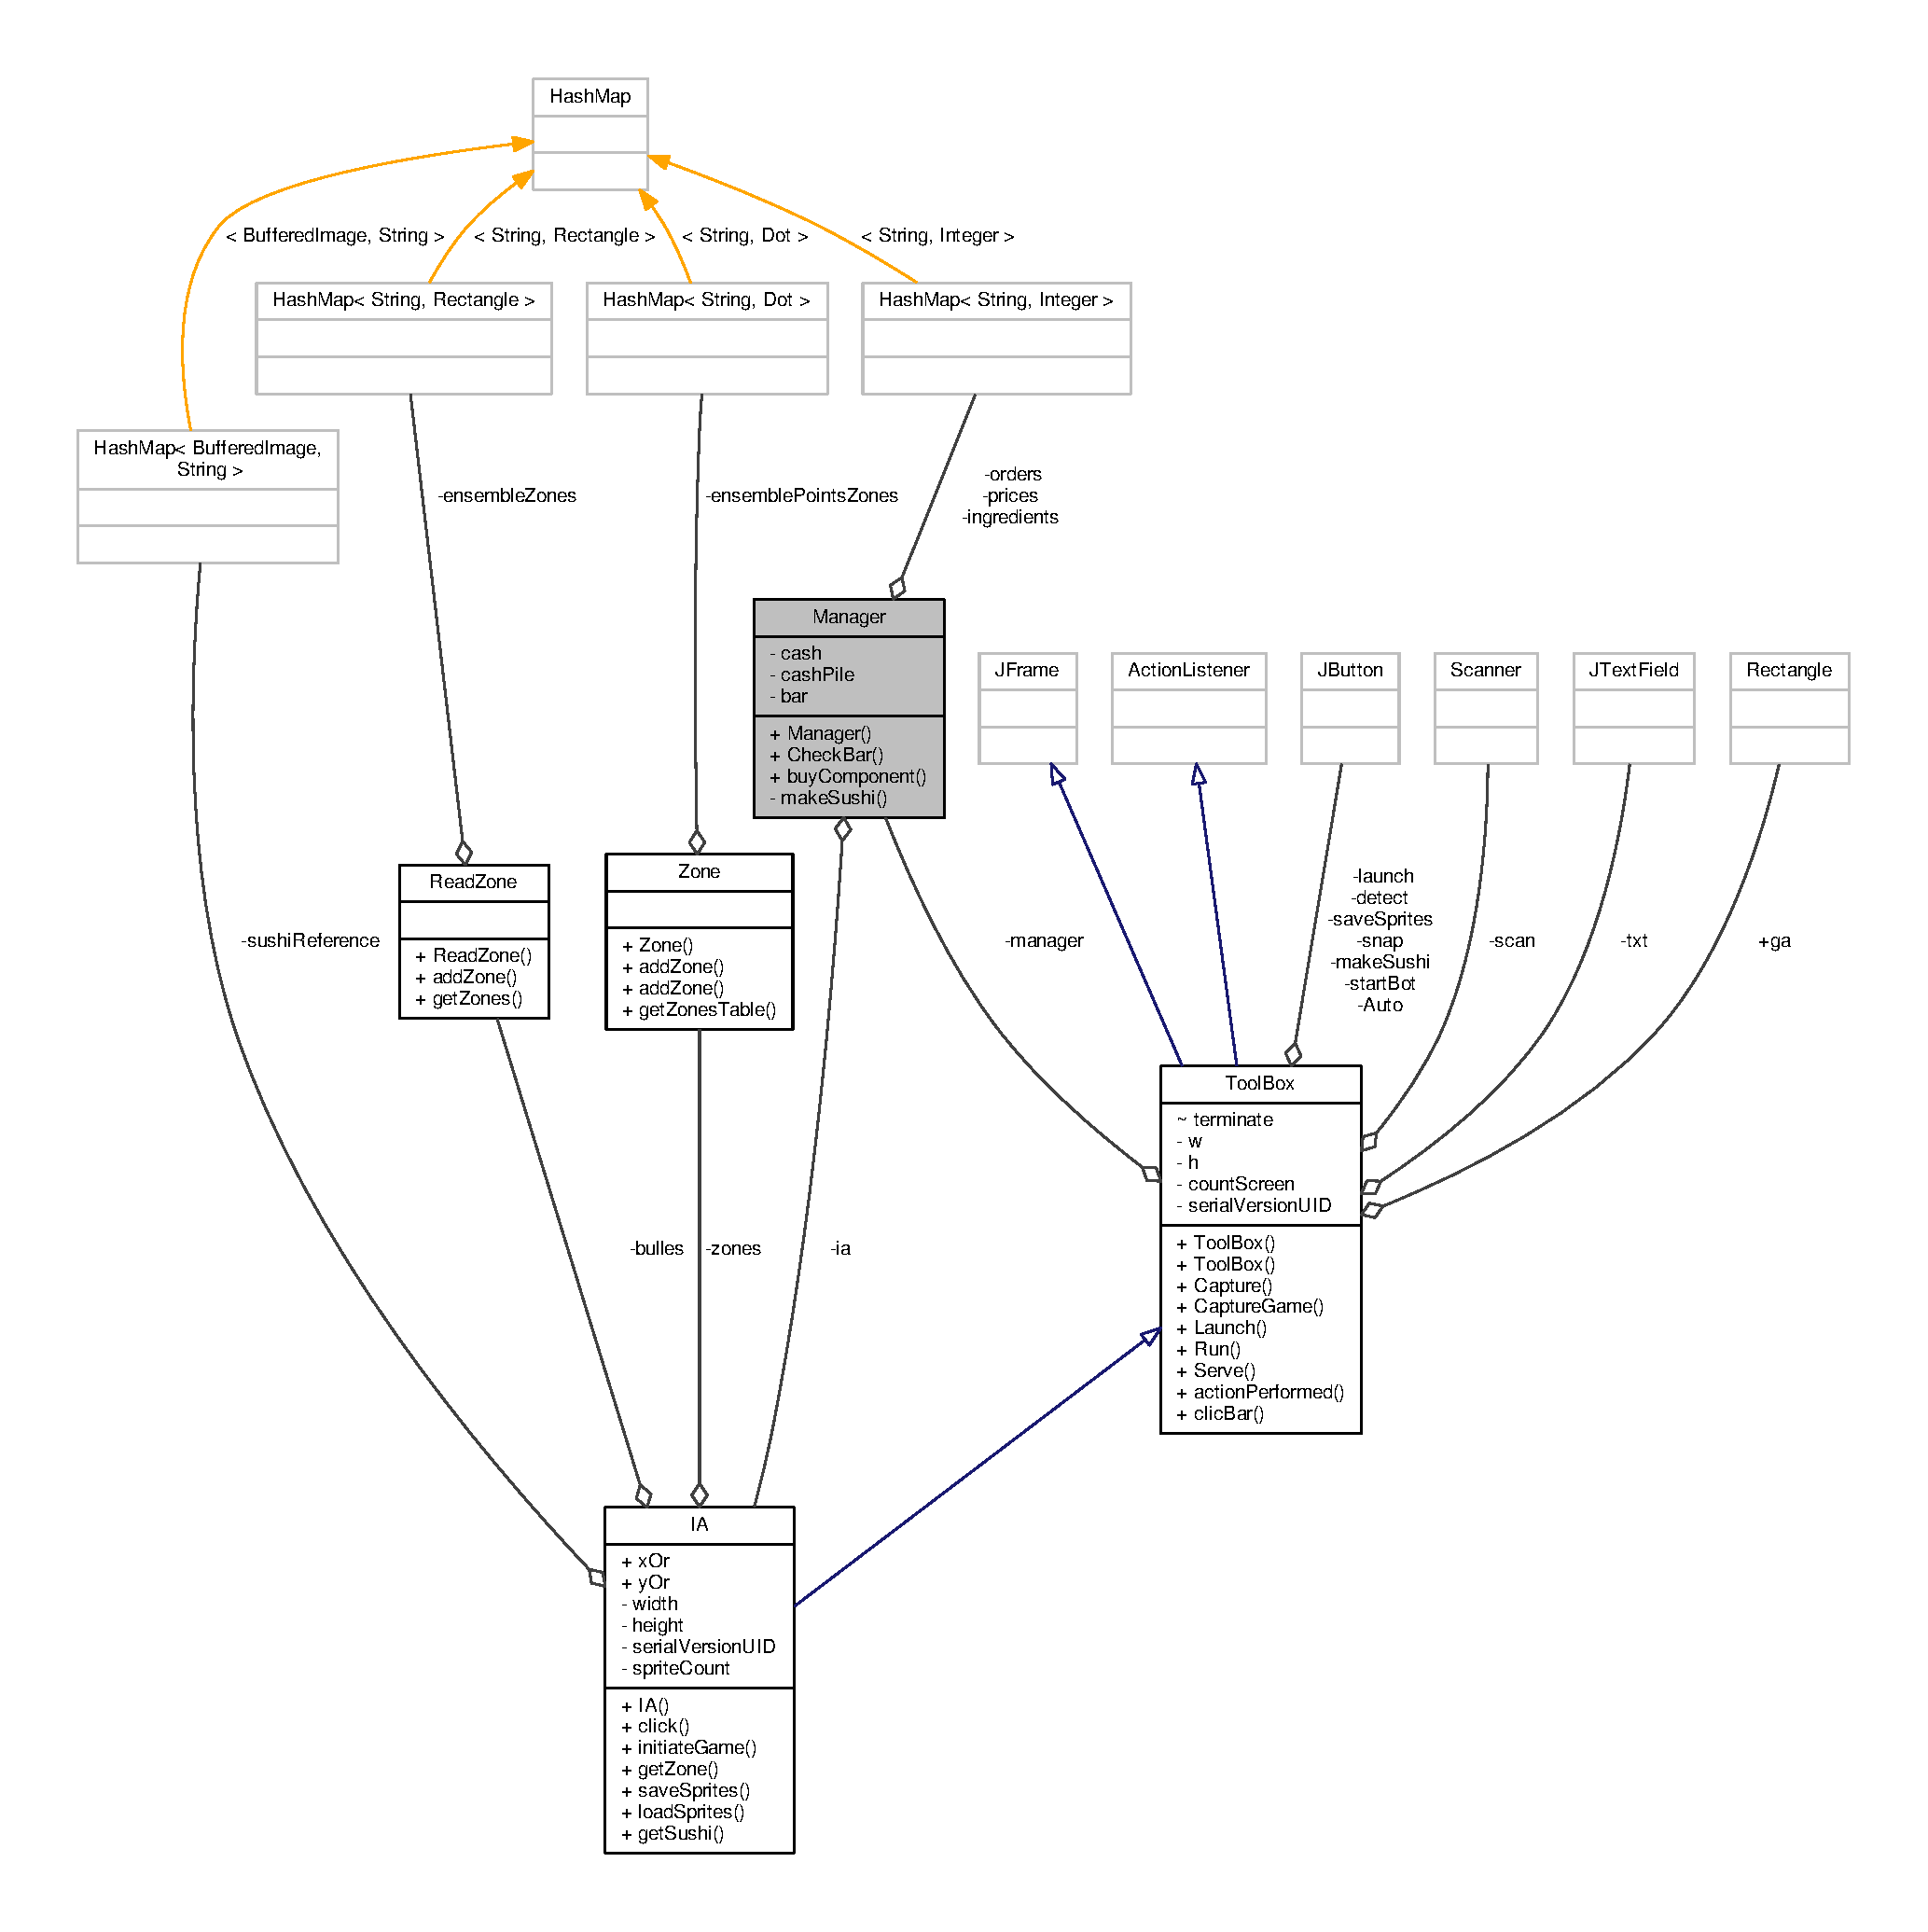
\includegraphics[width=350pt]{classManager__coll__graph}
\end{center}
\end{figure}
\subsubsection*{Fonctions membres publiques}
\begin{DoxyCompactItemize}
\item 
\hyperlink{classManager_ac6127238598371b4f44d1eed3b0c3b51}{Manager} ()  throws A\+W\+T\+Exception 
\item 
void \hyperlink{classManager_af4eb183d5dac5e9de89de6af2539cff7}{Check\+Bar} ()  throws A\+W\+T\+Exception, Interrupted\+Exception 
\item 
void \hyperlink{classManager_a724cfc01202d03838058a525454a1936}{buy\+Component} ()  throws A\+W\+T\+Exception, Interrupted\+Exception
\end{DoxyCompactItemize}
\subsubsection*{Fonctions membres privées}
\begin{DoxyCompactItemize}
\item 
Boolean \hyperlink{classManager_a2367553c5fc1fc67dceb06e0dad0e5b0}{make\+Sushi} (String sushi\+Name, int i)  throws A\+W\+T\+Exception, 			\+Interrupted\+Exception 
\end{DoxyCompactItemize}
\subsubsection*{Attributs privés}
\begin{DoxyCompactItemize}
\item 
\hyperlink{classIA}{I\+A} \hyperlink{classManager_a90957746b755371f0051a74b81f2827f}{ia}
\item 
Hash\+Map$<$ String, Integer $>$ \hyperlink{classManager_a731ab4f92babdcabb9a0e2e8ecc91b27}{ingredients}
\item 
Hash\+Map$<$ String, Integer $>$ \hyperlink{classManager_a4cb6296ce84b2fa63ff5726db1584238}{prices}
\item 
int \hyperlink{classManager_a50ed4ee3a6f3c444fab29330ba967ba4}{cash}
\item 
int\mbox{[}$\,$\mbox{]} \hyperlink{classManager_a7b0b5ed401cace73cb58b2510efc2508}{cash\+Pile}
\item 
Hash\+Map$<$ String, Integer $>$ \hyperlink{classManager_ab01a8b5bc2e4f1cc3abc9247bbf2ae6b}{orders}
\end{DoxyCompactItemize}
\subsubsection*{Attributs privés statiques}
\begin{DoxyCompactItemize}
\item 
static Boolean\mbox{[}$\,$\mbox{]} \hyperlink{classManager_a368d64d6025fecd75245c954cfa72e6a}{bar}
\end{DoxyCompactItemize}


\subsubsection{Documentation des constructeurs et destructeur}
\hypertarget{classManager_ac6127238598371b4f44d1eed3b0c3b51}{}\index{Manager@{Manager}!Manager@{Manager}}
\index{Manager@{Manager}!Manager@{Manager}}
\paragraph[{Manager}]{\setlength{\rightskip}{0pt plus 5cm}Manager.\+Manager (
\begin{DoxyParamCaption}
{}
\end{DoxyParamCaption}
) throws A\+W\+T\+Exception}\label{classManager_ac6127238598371b4f44d1eed3b0c3b51}


\subsubsection{Documentation des fonctions membres}
\hypertarget{classManager_a724cfc01202d03838058a525454a1936}{}\index{Manager@{Manager}!buy\+Component@{buy\+Component}}
\index{buy\+Component@{buy\+Component}!Manager@{Manager}}
\paragraph[{buy\+Component}]{\setlength{\rightskip}{0pt plus 5cm}void Manager.\+buy\+Component (
\begin{DoxyParamCaption}
{}
\end{DoxyParamCaption}
) throws A\+W\+T\+Exception, Interrupted\+Exception}\label{classManager_a724cfc01202d03838058a525454a1936}
\hypertarget{classManager_af4eb183d5dac5e9de89de6af2539cff7}{}\index{Manager@{Manager}!Check\+Bar@{Check\+Bar}}
\index{Check\+Bar@{Check\+Bar}!Manager@{Manager}}
\paragraph[{Check\+Bar}]{\setlength{\rightskip}{0pt plus 5cm}void Manager.\+Check\+Bar (
\begin{DoxyParamCaption}
{}
\end{DoxyParamCaption}
) throws A\+W\+T\+Exception, Interrupted\+Exception}\label{classManager_af4eb183d5dac5e9de89de6af2539cff7}


Référencé par Tool\+Box.\+Serve().

\hypertarget{classManager_a2367553c5fc1fc67dceb06e0dad0e5b0}{}\index{Manager@{Manager}!make\+Sushi@{make\+Sushi}}
\index{make\+Sushi@{make\+Sushi}!Manager@{Manager}}
\paragraph[{make\+Sushi}]{\setlength{\rightskip}{0pt plus 5cm}Boolean Manager.\+make\+Sushi (
\begin{DoxyParamCaption}
\item[{String}]{sushi\+Name, }
\item[{int}]{i}
\end{DoxyParamCaption}
) throws A\+W\+T\+Exception, 			Interrupted\+Exception\hspace{0.3cm}{\ttfamily [private]}}\label{classManager_a2367553c5fc1fc67dceb06e0dad0e5b0}


\subsubsection{Documentation des données membres}
\hypertarget{classManager_a368d64d6025fecd75245c954cfa72e6a}{}\index{Manager@{Manager}!bar@{bar}}
\index{bar@{bar}!Manager@{Manager}}
\paragraph[{bar}]{\setlength{\rightskip}{0pt plus 5cm}Boolean \mbox{[}$\,$\mbox{]} Manager.\+bar\hspace{0.3cm}{\ttfamily [static]}, {\ttfamily [private]}}\label{classManager_a368d64d6025fecd75245c954cfa72e6a}
\hypertarget{classManager_a50ed4ee3a6f3c444fab29330ba967ba4}{}\index{Manager@{Manager}!cash@{cash}}
\index{cash@{cash}!Manager@{Manager}}
\paragraph[{cash}]{\setlength{\rightskip}{0pt plus 5cm}int Manager.\+cash\hspace{0.3cm}{\ttfamily [private]}}\label{classManager_a50ed4ee3a6f3c444fab29330ba967ba4}
\hypertarget{classManager_a7b0b5ed401cace73cb58b2510efc2508}{}\index{Manager@{Manager}!cash\+Pile@{cash\+Pile}}
\index{cash\+Pile@{cash\+Pile}!Manager@{Manager}}
\paragraph[{cash\+Pile}]{\setlength{\rightskip}{0pt plus 5cm}int \mbox{[}$\,$\mbox{]} Manager.\+cash\+Pile\hspace{0.3cm}{\ttfamily [private]}}\label{classManager_a7b0b5ed401cace73cb58b2510efc2508}
\hypertarget{classManager_a90957746b755371f0051a74b81f2827f}{}\index{Manager@{Manager}!ia@{ia}}
\index{ia@{ia}!Manager@{Manager}}
\paragraph[{ia}]{\setlength{\rightskip}{0pt plus 5cm}{\bf I\+A} Manager.\+ia\hspace{0.3cm}{\ttfamily [private]}}\label{classManager_a90957746b755371f0051a74b81f2827f}
\hypertarget{classManager_a731ab4f92babdcabb9a0e2e8ecc91b27}{}\index{Manager@{Manager}!ingredients@{ingredients}}
\index{ingredients@{ingredients}!Manager@{Manager}}
\paragraph[{ingredients}]{\setlength{\rightskip}{0pt plus 5cm}Hash\+Map$<$String, Integer$>$ Manager.\+ingredients\hspace{0.3cm}{\ttfamily [private]}}\label{classManager_a731ab4f92babdcabb9a0e2e8ecc91b27}
\hypertarget{classManager_ab01a8b5bc2e4f1cc3abc9247bbf2ae6b}{}\index{Manager@{Manager}!orders@{orders}}
\index{orders@{orders}!Manager@{Manager}}
\paragraph[{orders}]{\setlength{\rightskip}{0pt plus 5cm}Hash\+Map$<$String, Integer$>$ Manager.\+orders\hspace{0.3cm}{\ttfamily [private]}}\label{classManager_ab01a8b5bc2e4f1cc3abc9247bbf2ae6b}
\hypertarget{classManager_a4cb6296ce84b2fa63ff5726db1584238}{}\index{Manager@{Manager}!prices@{prices}}
\index{prices@{prices}!Manager@{Manager}}
\paragraph[{prices}]{\setlength{\rightskip}{0pt plus 5cm}Hash\+Map$<$String, Integer$>$ Manager.\+prices\hspace{0.3cm}{\ttfamily [private]}}\label{classManager_a4cb6296ce84b2fa63ff5726db1584238}


La documentation de cette classe a été générée à partir du fichier suivant \+:\begin{DoxyCompactItemize}
\item 
\hyperlink{oldCode_2Manager_8java}{old\+Code/\+Manager.\+java}\end{DoxyCompactItemize}

\hypertarget{classSushis_1_1src_1_1Manager}{}\subsection{Référence de la classe Sushis.\+src.\+Manager}
\label{classSushis_1_1src_1_1Manager}\index{Sushis.\+src.\+Manager@{Sushis.\+src.\+Manager}}


Graphe de collaboration de Sushis.\+src.\+Manager\+:\nopagebreak
\begin{figure}[H]
\begin{center}
\leavevmode
\includegraphics[width=350pt]{classSushis_1_1src_1_1Manager__coll__graph}
\end{center}
\end{figure}
\subsubsection*{Fonctions membres publiques}
\begin{DoxyCompactItemize}
\item 
\hyperlink{classSushis_1_1src_1_1Manager_ad3c6eb65a2468a2afde378e5e4635aea}{Manager} ()  throws A\+W\+T\+Exception 
\item 
void \hyperlink{classSushis_1_1src_1_1Manager_a76009c42816f2888b98c4d051dda02c9}{Check\+Bar} ()  throws A\+W\+T\+Exception, Interrupted\+Exception 
\end{DoxyCompactItemize}
\subsubsection*{Fonctions membres privées}
\begin{DoxyCompactItemize}
\item 
Boolean \hyperlink{classSushis_1_1src_1_1Manager_ab52d513835dbbe38676a93431e04dd46}{make\+Sushi} (String sushi\+Name)  throws A\+W\+T\+Exception, 			\+Interrupted\+Exception 
\end{DoxyCompactItemize}
\subsubsection*{Attributs privés}
\begin{DoxyCompactItemize}
\item 
\hyperlink{classSushis_1_1src_1_1IA}{I\+A} \hyperlink{classSushis_1_1src_1_1Manager_a1b807b964e5abf15e84f7bec47b3d7d5}{ia}
\item 
Hash\+Map$<$ String, Integer $>$ \hyperlink{classSushis_1_1src_1_1Manager_aeb7c5ea92c4658cf9001a6a3c0f8022c}{ingredients}
\item 
int \hyperlink{classSushis_1_1src_1_1Manager_ae59b41a9619054cec5ce56cbbde77f30}{cash}
\end{DoxyCompactItemize}
\subsubsection*{Attributs privés statiques}
\begin{DoxyCompactItemize}
\item 
static Boolean\mbox{[}$\,$\mbox{]} \hyperlink{classSushis_1_1src_1_1Manager_ae135bee329f98bc9bad9ca62f6bb3d92}{bar}
\end{DoxyCompactItemize}


\subsubsection{Documentation des constructeurs et destructeur}
\hypertarget{classSushis_1_1src_1_1Manager_ad3c6eb65a2468a2afde378e5e4635aea}{}\index{Sushis\+::src\+::\+Manager@{Sushis\+::src\+::\+Manager}!Manager@{Manager}}
\index{Manager@{Manager}!Sushis\+::src\+::\+Manager@{Sushis\+::src\+::\+Manager}}
\paragraph[{Manager}]{\setlength{\rightskip}{0pt plus 5cm}Sushis.\+src.\+Manager.\+Manager (
\begin{DoxyParamCaption}
{}
\end{DoxyParamCaption}
) throws A\+W\+T\+Exception}\label{classSushis_1_1src_1_1Manager_ad3c6eb65a2468a2afde378e5e4635aea}


\subsubsection{Documentation des fonctions membres}
\hypertarget{classSushis_1_1src_1_1Manager_a76009c42816f2888b98c4d051dda02c9}{}\index{Sushis\+::src\+::\+Manager@{Sushis\+::src\+::\+Manager}!Check\+Bar@{Check\+Bar}}
\index{Check\+Bar@{Check\+Bar}!Sushis\+::src\+::\+Manager@{Sushis\+::src\+::\+Manager}}
\paragraph[{Check\+Bar}]{\setlength{\rightskip}{0pt plus 5cm}void Sushis.\+src.\+Manager.\+Check\+Bar (
\begin{DoxyParamCaption}
{}
\end{DoxyParamCaption}
) throws A\+W\+T\+Exception, Interrupted\+Exception}\label{classSushis_1_1src_1_1Manager_a76009c42816f2888b98c4d051dda02c9}


Référencé par Sushis.\+src.\+Tool\+Box.\+Serve().

\hypertarget{classSushis_1_1src_1_1Manager_ab52d513835dbbe38676a93431e04dd46}{}\index{Sushis\+::src\+::\+Manager@{Sushis\+::src\+::\+Manager}!make\+Sushi@{make\+Sushi}}
\index{make\+Sushi@{make\+Sushi}!Sushis\+::src\+::\+Manager@{Sushis\+::src\+::\+Manager}}
\paragraph[{make\+Sushi}]{\setlength{\rightskip}{0pt plus 5cm}Boolean Sushis.\+src.\+Manager.\+make\+Sushi (
\begin{DoxyParamCaption}
\item[{String}]{sushi\+Name}
\end{DoxyParamCaption}
) throws A\+W\+T\+Exception, 			Interrupted\+Exception\hspace{0.3cm}{\ttfamily [private]}}\label{classSushis_1_1src_1_1Manager_ab52d513835dbbe38676a93431e04dd46}


Référencé par Sushis.\+src.\+Manager.\+Check\+Bar().



\subsubsection{Documentation des données membres}
\hypertarget{classSushis_1_1src_1_1Manager_ae135bee329f98bc9bad9ca62f6bb3d92}{}\index{Sushis\+::src\+::\+Manager@{Sushis\+::src\+::\+Manager}!bar@{bar}}
\index{bar@{bar}!Sushis\+::src\+::\+Manager@{Sushis\+::src\+::\+Manager}}
\paragraph[{bar}]{\setlength{\rightskip}{0pt plus 5cm}Boolean \mbox{[}$\,$\mbox{]} Sushis.\+src.\+Manager.\+bar\hspace{0.3cm}{\ttfamily [static]}, {\ttfamily [private]}}\label{classSushis_1_1src_1_1Manager_ae135bee329f98bc9bad9ca62f6bb3d92}
\hypertarget{classSushis_1_1src_1_1Manager_ae59b41a9619054cec5ce56cbbde77f30}{}\index{Sushis\+::src\+::\+Manager@{Sushis\+::src\+::\+Manager}!cash@{cash}}
\index{cash@{cash}!Sushis\+::src\+::\+Manager@{Sushis\+::src\+::\+Manager}}
\paragraph[{cash}]{\setlength{\rightskip}{0pt plus 5cm}int Sushis.\+src.\+Manager.\+cash\hspace{0.3cm}{\ttfamily [private]}}\label{classSushis_1_1src_1_1Manager_ae59b41a9619054cec5ce56cbbde77f30}
\hypertarget{classSushis_1_1src_1_1Manager_a1b807b964e5abf15e84f7bec47b3d7d5}{}\index{Sushis\+::src\+::\+Manager@{Sushis\+::src\+::\+Manager}!ia@{ia}}
\index{ia@{ia}!Sushis\+::src\+::\+Manager@{Sushis\+::src\+::\+Manager}}
\paragraph[{ia}]{\setlength{\rightskip}{0pt plus 5cm}{\bf I\+A} Sushis.\+src.\+Manager.\+ia\hspace{0.3cm}{\ttfamily [private]}}\label{classSushis_1_1src_1_1Manager_a1b807b964e5abf15e84f7bec47b3d7d5}
\hypertarget{classSushis_1_1src_1_1Manager_aeb7c5ea92c4658cf9001a6a3c0f8022c}{}\index{Sushis\+::src\+::\+Manager@{Sushis\+::src\+::\+Manager}!ingredients@{ingredients}}
\index{ingredients@{ingredients}!Sushis\+::src\+::\+Manager@{Sushis\+::src\+::\+Manager}}
\paragraph[{ingredients}]{\setlength{\rightskip}{0pt plus 5cm}Hash\+Map$<$String, Integer$>$ Sushis.\+src.\+Manager.\+ingredients\hspace{0.3cm}{\ttfamily [private]}}\label{classSushis_1_1src_1_1Manager_aeb7c5ea92c4658cf9001a6a3c0f8022c}


La documentation de cette classe a été générée à partir du fichier suivant \+:\begin{DoxyCompactItemize}
\item 
\hyperlink{projet_2Sushis_2src_2Manager_8java}{projet/\+Sushis/src/\+Manager.\+java}\end{DoxyCompactItemize}

\hypertarget{classmain_1_1Manager}{}\subsection{Référence de la classe main.\+Manager}
\label{classmain_1_1Manager}\index{main.\+Manager@{main.\+Manager}}


Graphe de collaboration de main.\+Manager\+:\nopagebreak
\begin{figure}[H]
\begin{center}
\leavevmode
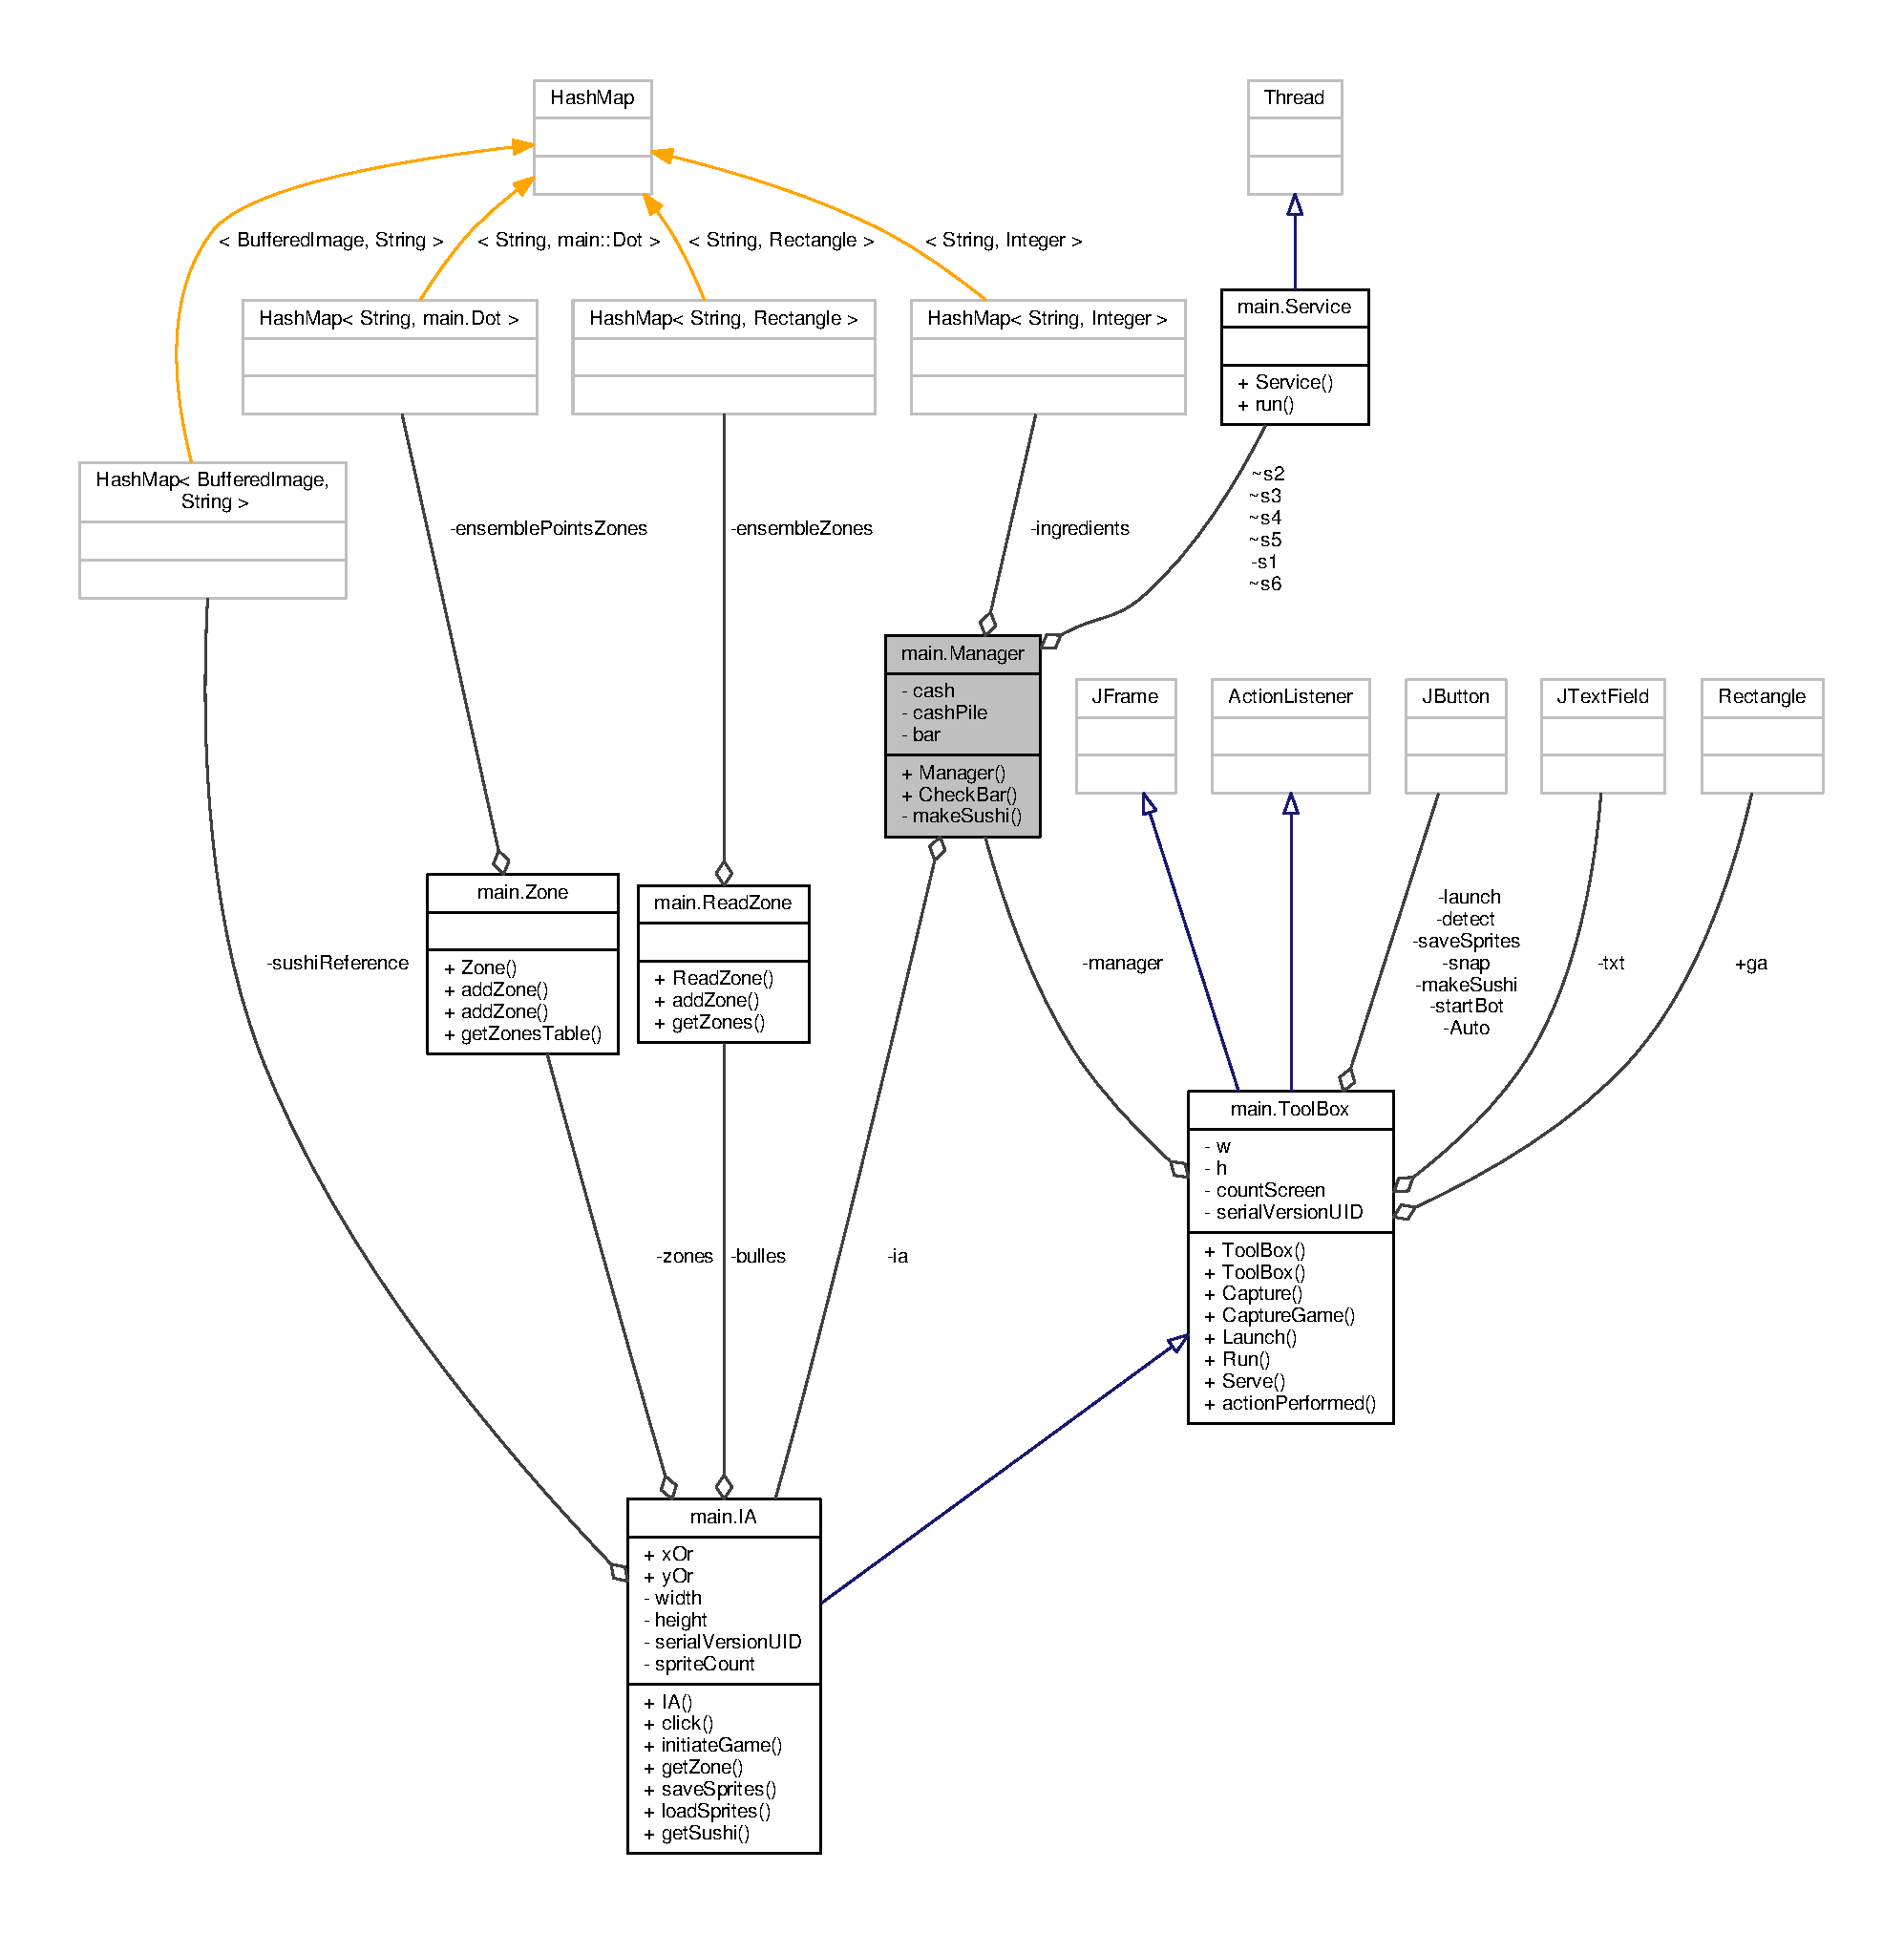
\includegraphics[width=350pt]{classmain_1_1Manager__coll__graph}
\end{center}
\end{figure}
\subsubsection*{Fonctions membres publiques}
\begin{DoxyCompactItemize}
\item 
\hyperlink{classmain_1_1Manager_ae258b5aecf0ef1f62a2f2e50a93fd7e6}{Manager} ()  throws A\+W\+T\+Exception 
\item 
void \hyperlink{classmain_1_1Manager_a09b65c1d252dfc883dc45c4e20460f3f}{Check\+Bar} ()  throws A\+W\+T\+Exception, Interrupted\+Exception 
\end{DoxyCompactItemize}
\subsubsection*{Attributs de paquetage}
\begin{DoxyCompactItemize}
\item 
\hyperlink{classmain_1_1Service}{Service} \hyperlink{classmain_1_1Manager_adb7111921777e8df2511b73b69c7af05}{s2}
\item 
\hyperlink{classmain_1_1Service}{Service} \hyperlink{classmain_1_1Manager_a853a3f26b9a69b2dc7f96055a832ddbd}{s3}
\item 
\hyperlink{classmain_1_1Service}{Service} \hyperlink{classmain_1_1Manager_a9735c9ed38407fa5cc20623372807a01}{s4}
\item 
\hyperlink{classmain_1_1Service}{Service} \hyperlink{classmain_1_1Manager_abc0528186764144b702030cdbcb409df}{s5}
\item 
\hyperlink{classmain_1_1Service}{Service} \hyperlink{classmain_1_1Manager_a32e046e37c048665d90d769f3e0b0bac}{s6}
\end{DoxyCompactItemize}
\subsubsection*{Fonctions membres privées}
\begin{DoxyCompactItemize}
\item 
Boolean \hyperlink{classmain_1_1Manager_a4088d1c9a36a219349959e4ab7184eb9}{make\+Sushi} (String sushi\+Name)  throws A\+W\+T\+Exception, 			\+Interrupted\+Exception 
\end{DoxyCompactItemize}
\subsubsection*{Attributs privés}
\begin{DoxyCompactItemize}
\item 
\hyperlink{classmain_1_1IA}{I\+A} \hyperlink{classmain_1_1Manager_a2ec66c16cb2670f76ad9f7d941761221}{ia}
\item 
Hash\+Map$<$ String, Integer $>$ \hyperlink{classmain_1_1Manager_a20b4db237b6744ed2b6974af96acacff}{ingredients}
\item 
int \hyperlink{classmain_1_1Manager_a1d8a267adacd2d29d6d1954e59b56948}{cash}
\item 
int \hyperlink{classmain_1_1Manager_aba1943680dbaf8eba8576dc54d56bda8}{cash\+Pile}
\item 
\hyperlink{classmain_1_1Service}{Service} \hyperlink{classmain_1_1Manager_a6d675483c641fbd495900af6a2d48868}{s1}
\end{DoxyCompactItemize}
\subsubsection*{Attributs privés statiques}
\begin{DoxyCompactItemize}
\item 
static Boolean\mbox{[}$\,$\mbox{]} \hyperlink{classmain_1_1Manager_aaf565d03e7bb7b7e99358425ff78b478}{bar}
\end{DoxyCompactItemize}


\subsubsection{Documentation des constructeurs et destructeur}
\hypertarget{classmain_1_1Manager_ae258b5aecf0ef1f62a2f2e50a93fd7e6}{}\index{main\+::\+Manager@{main\+::\+Manager}!Manager@{Manager}}
\index{Manager@{Manager}!main\+::\+Manager@{main\+::\+Manager}}
\paragraph[{Manager}]{\setlength{\rightskip}{0pt plus 5cm}main.\+Manager.\+Manager (
\begin{DoxyParamCaption}
{}
\end{DoxyParamCaption}
) throws A\+W\+T\+Exception}\label{classmain_1_1Manager_ae258b5aecf0ef1f62a2f2e50a93fd7e6}


\subsubsection{Documentation des fonctions membres}
\hypertarget{classmain_1_1Manager_a09b65c1d252dfc883dc45c4e20460f3f}{}\index{main\+::\+Manager@{main\+::\+Manager}!Check\+Bar@{Check\+Bar}}
\index{Check\+Bar@{Check\+Bar}!main\+::\+Manager@{main\+::\+Manager}}
\paragraph[{Check\+Bar}]{\setlength{\rightskip}{0pt plus 5cm}void main.\+Manager.\+Check\+Bar (
\begin{DoxyParamCaption}
{}
\end{DoxyParamCaption}
) throws A\+W\+T\+Exception, Interrupted\+Exception}\label{classmain_1_1Manager_a09b65c1d252dfc883dc45c4e20460f3f}


Référencé par main.\+Tool\+Box.\+Serve().

\hypertarget{classmain_1_1Manager_a4088d1c9a36a219349959e4ab7184eb9}{}\index{main\+::\+Manager@{main\+::\+Manager}!make\+Sushi@{make\+Sushi}}
\index{make\+Sushi@{make\+Sushi}!main\+::\+Manager@{main\+::\+Manager}}
\paragraph[{make\+Sushi}]{\setlength{\rightskip}{0pt plus 5cm}Boolean main.\+Manager.\+make\+Sushi (
\begin{DoxyParamCaption}
\item[{String}]{sushi\+Name}
\end{DoxyParamCaption}
) throws A\+W\+T\+Exception, 			Interrupted\+Exception\hspace{0.3cm}{\ttfamily [private]}}\label{classmain_1_1Manager_a4088d1c9a36a219349959e4ab7184eb9}


Référencé par main.\+Manager.\+Check\+Bar().



\subsubsection{Documentation des données membres}
\hypertarget{classmain_1_1Manager_aaf565d03e7bb7b7e99358425ff78b478}{}\index{main\+::\+Manager@{main\+::\+Manager}!bar@{bar}}
\index{bar@{bar}!main\+::\+Manager@{main\+::\+Manager}}
\paragraph[{bar}]{\setlength{\rightskip}{0pt plus 5cm}Boolean \mbox{[}$\,$\mbox{]} main.\+Manager.\+bar\hspace{0.3cm}{\ttfamily [static]}, {\ttfamily [private]}}\label{classmain_1_1Manager_aaf565d03e7bb7b7e99358425ff78b478}
\hypertarget{classmain_1_1Manager_a1d8a267adacd2d29d6d1954e59b56948}{}\index{main\+::\+Manager@{main\+::\+Manager}!cash@{cash}}
\index{cash@{cash}!main\+::\+Manager@{main\+::\+Manager}}
\paragraph[{cash}]{\setlength{\rightskip}{0pt plus 5cm}int main.\+Manager.\+cash\hspace{0.3cm}{\ttfamily [private]}}\label{classmain_1_1Manager_a1d8a267adacd2d29d6d1954e59b56948}
\hypertarget{classmain_1_1Manager_aba1943680dbaf8eba8576dc54d56bda8}{}\index{main\+::\+Manager@{main\+::\+Manager}!cash\+Pile@{cash\+Pile}}
\index{cash\+Pile@{cash\+Pile}!main\+::\+Manager@{main\+::\+Manager}}
\paragraph[{cash\+Pile}]{\setlength{\rightskip}{0pt plus 5cm}int main.\+Manager.\+cash\+Pile\hspace{0.3cm}{\ttfamily [private]}}\label{classmain_1_1Manager_aba1943680dbaf8eba8576dc54d56bda8}
\hypertarget{classmain_1_1Manager_a2ec66c16cb2670f76ad9f7d941761221}{}\index{main\+::\+Manager@{main\+::\+Manager}!ia@{ia}}
\index{ia@{ia}!main\+::\+Manager@{main\+::\+Manager}}
\paragraph[{ia}]{\setlength{\rightskip}{0pt plus 5cm}{\bf I\+A} main.\+Manager.\+ia\hspace{0.3cm}{\ttfamily [private]}}\label{classmain_1_1Manager_a2ec66c16cb2670f76ad9f7d941761221}
\hypertarget{classmain_1_1Manager_a20b4db237b6744ed2b6974af96acacff}{}\index{main\+::\+Manager@{main\+::\+Manager}!ingredients@{ingredients}}
\index{ingredients@{ingredients}!main\+::\+Manager@{main\+::\+Manager}}
\paragraph[{ingredients}]{\setlength{\rightskip}{0pt plus 5cm}Hash\+Map$<$String, Integer$>$ main.\+Manager.\+ingredients\hspace{0.3cm}{\ttfamily [private]}}\label{classmain_1_1Manager_a20b4db237b6744ed2b6974af96acacff}
\hypertarget{classmain_1_1Manager_a6d675483c641fbd495900af6a2d48868}{}\index{main\+::\+Manager@{main\+::\+Manager}!s1@{s1}}
\index{s1@{s1}!main\+::\+Manager@{main\+::\+Manager}}
\paragraph[{s1}]{\setlength{\rightskip}{0pt plus 5cm}{\bf Service} main.\+Manager.\+s1\hspace{0.3cm}{\ttfamily [private]}}\label{classmain_1_1Manager_a6d675483c641fbd495900af6a2d48868}
\hypertarget{classmain_1_1Manager_adb7111921777e8df2511b73b69c7af05}{}\index{main\+::\+Manager@{main\+::\+Manager}!s2@{s2}}
\index{s2@{s2}!main\+::\+Manager@{main\+::\+Manager}}
\paragraph[{s2}]{\setlength{\rightskip}{0pt plus 5cm}{\bf Service} main.\+Manager.\+s2\hspace{0.3cm}{\ttfamily [package]}}\label{classmain_1_1Manager_adb7111921777e8df2511b73b69c7af05}
\hypertarget{classmain_1_1Manager_a853a3f26b9a69b2dc7f96055a832ddbd}{}\index{main\+::\+Manager@{main\+::\+Manager}!s3@{s3}}
\index{s3@{s3}!main\+::\+Manager@{main\+::\+Manager}}
\paragraph[{s3}]{\setlength{\rightskip}{0pt plus 5cm}{\bf Service} main.\+Manager.\+s3\hspace{0.3cm}{\ttfamily [package]}}\label{classmain_1_1Manager_a853a3f26b9a69b2dc7f96055a832ddbd}
\hypertarget{classmain_1_1Manager_a9735c9ed38407fa5cc20623372807a01}{}\index{main\+::\+Manager@{main\+::\+Manager}!s4@{s4}}
\index{s4@{s4}!main\+::\+Manager@{main\+::\+Manager}}
\paragraph[{s4}]{\setlength{\rightskip}{0pt plus 5cm}{\bf Service} main.\+Manager.\+s4\hspace{0.3cm}{\ttfamily [package]}}\label{classmain_1_1Manager_a9735c9ed38407fa5cc20623372807a01}
\hypertarget{classmain_1_1Manager_abc0528186764144b702030cdbcb409df}{}\index{main\+::\+Manager@{main\+::\+Manager}!s5@{s5}}
\index{s5@{s5}!main\+::\+Manager@{main\+::\+Manager}}
\paragraph[{s5}]{\setlength{\rightskip}{0pt plus 5cm}{\bf Service} main.\+Manager.\+s5\hspace{0.3cm}{\ttfamily [package]}}\label{classmain_1_1Manager_abc0528186764144b702030cdbcb409df}
\hypertarget{classmain_1_1Manager_a32e046e37c048665d90d769f3e0b0bac}{}\index{main\+::\+Manager@{main\+::\+Manager}!s6@{s6}}
\index{s6@{s6}!main\+::\+Manager@{main\+::\+Manager}}
\paragraph[{s6}]{\setlength{\rightskip}{0pt plus 5cm}{\bf Service} main.\+Manager.\+s6\hspace{0.3cm}{\ttfamily [package]}}\label{classmain_1_1Manager_a32e046e37c048665d90d769f3e0b0bac}


La documentation de cette classe a été générée à partir du fichier suivant \+:\begin{DoxyCompactItemize}
\item 
\hyperlink{main_2Manager_8java}{main/\+Manager.\+java}\end{DoxyCompactItemize}

\hypertarget{classTestSushi_1_1src_1_1Suchi_1_1Onigiri}{}\subsection{Référence de la classe Test\+Sushi.\+src.\+Suchi.\+Onigiri}
\label{classTestSushi_1_1src_1_1Suchi_1_1Onigiri}\index{Test\+Sushi.\+src.\+Suchi.\+Onigiri@{Test\+Sushi.\+src.\+Suchi.\+Onigiri}}


Graphe d\textquotesingle{}héritage de Test\+Sushi.\+src.\+Suchi.\+Onigiri\+:\nopagebreak
\begin{figure}[H]
\begin{center}
\leavevmode
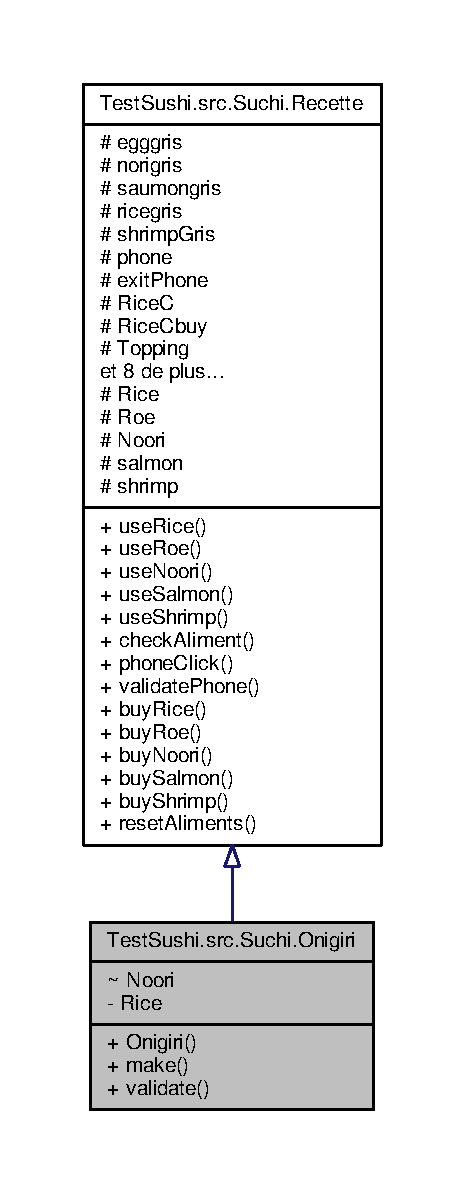
\includegraphics[height=550pt]{classTestSushi_1_1src_1_1Suchi_1_1Onigiri__inherit__graph}
\end{center}
\end{figure}


Graphe de collaboration de Test\+Sushi.\+src.\+Suchi.\+Onigiri\+:\nopagebreak
\begin{figure}[H]
\begin{center}
\leavevmode
\includegraphics[height=550pt]{classTestSushi_1_1src_1_1Suchi_1_1Onigiri__coll__graph}
\end{center}
\end{figure}
\subsubsection*{Fonctions membres publiques}
\begin{DoxyCompactItemize}
\item 
\hyperlink{classTestSushi_1_1src_1_1Suchi_1_1Onigiri_a4f279ca850ccceb05576b8006ea303b6}{Onigiri} ()  throws A\+W\+T\+Exception, Interrupted\+Exception
\begin{DoxyCompactList}\small\item\em Constructeur pour créer un onigri. \end{DoxyCompactList}\item 
void \hyperlink{classTestSushi_1_1src_1_1Suchi_1_1Onigiri_a5ed4d63c69015a765597a58d83e7a8f5}{make} ()  throws A\+W\+T\+Exception, Interrupted\+Exception
\item 
void \hyperlink{classTestSushi_1_1src_1_1Suchi_1_1Onigiri_a65d8de2ad6a3deef9f409271bd7320ce}{validate} ()  throws A\+W\+T\+Exception, Interrupted\+Exception 
\item 
void \hyperlink{classTestSushi_1_1src_1_1Suchi_1_1Recette_a2d78a4575d1295e34210e2f77c01f3f3}{use\+Rice} ()  throws A\+W\+T\+Exception, Interrupted\+Exception
\item 
void \hyperlink{classTestSushi_1_1src_1_1Suchi_1_1Recette_a8967a205e78d02ef7c30fd435fbaa0af}{use\+Roe} ()  throws A\+W\+T\+Exception, Interrupted\+Exception
\item 
void \hyperlink{classTestSushi_1_1src_1_1Suchi_1_1Recette_a10bfe3c71750c84144203a7aa2c341ee}{use\+Noori} ()  throws A\+W\+T\+Exception, Interrupted\+Exception
\item 
void \hyperlink{classTestSushi_1_1src_1_1Suchi_1_1Recette_a87cd9338767df0e5db88e6005f1da984}{use\+Salmon} ()  throws A\+W\+T\+Exception, Interrupted\+Exception
\item 
void \hyperlink{classTestSushi_1_1src_1_1Suchi_1_1Recette_ab2c165554830ba84a392765621604d44}{use\+Shrimp} ()  throws A\+W\+T\+Exception, Interrupted\+Exception
\item 
void \hyperlink{classTestSushi_1_1src_1_1Suchi_1_1Recette_a83f9f5fb6bfe2691974a5e35386e7b8a}{check\+Aliment} ()  throws A\+W\+T\+Exception, Interrupted\+Exception
\item 
void \hyperlink{classTestSushi_1_1src_1_1Suchi_1_1Recette_ad94006ea131c2379a14c50eec870b69b}{phone\+Click} ()  throws A\+W\+T\+Exception, Interrupted\+Exception
\item 
void \hyperlink{classTestSushi_1_1src_1_1Suchi_1_1Recette_a33f0912e1212b01ea1b3787bed28f0fe}{validate\+Phone} ()  throws A\+W\+T\+Exception
\item 
void \hyperlink{classTestSushi_1_1src_1_1Suchi_1_1Recette_aa0fc4c335f6ab3f905f63a16902a6379}{buy\+Rice} ()  throws A\+W\+T\+Exception, Interrupted\+Exception
\item 
void \hyperlink{classTestSushi_1_1src_1_1Suchi_1_1Recette_ad874ba9daf68328d6b65b09e6f16003e}{buy\+Roe} ()  throws A\+W\+T\+Exception, Interrupted\+Exception
\item 
void \hyperlink{classTestSushi_1_1src_1_1Suchi_1_1Recette_a5602befaaef8858b75c131e50f7cf91d}{buy\+Noori} ()  throws A\+W\+T\+Exception, Interrupted\+Exception
\item 
void \hyperlink{classTestSushi_1_1src_1_1Suchi_1_1Recette_a64cf6254490e04e9e8031d564a4a0ea3}{buy\+Salmon} ()  throws A\+W\+T\+Exception, Interrupted\+Exception
\item 
void \hyperlink{classTestSushi_1_1src_1_1Suchi_1_1Recette_a0d15202c729b3c6b2bb699de4137d551}{buy\+Shrimp} ()  throws A\+W\+T\+Exception, Interrupted\+Exception
\end{DoxyCompactItemize}
\subsubsection*{Fonctions membres publiques statiques}
\begin{DoxyCompactItemize}
\item 
static void \hyperlink{classTestSushi_1_1src_1_1Suchi_1_1Recette_aef7faa1aea5f8aeb869c612af16e4e62}{reset\+Aliments} ()
\end{DoxyCompactItemize}
\subsubsection*{Attributs protégés}
\begin{DoxyCompactItemize}
\item 
final String \hyperlink{classTestSushi_1_1src_1_1Suchi_1_1Recette_a14892e43d9ed57350effdf3ed1bddb8a}{egggris} = \char`\"{}sprites/egg\+Gris.\+png\char`\"{}
\item 
final String \hyperlink{classTestSushi_1_1src_1_1Suchi_1_1Recette_a774959efa525787a162778df37770b7c}{norigris} = \char`\"{}sprites/nori\+Gris.\+png\char`\"{}
\item 
final String \hyperlink{classTestSushi_1_1src_1_1Suchi_1_1Recette_aea59cc2a5f6bc21ec36690a5bf1eb38c}{saumongris} =\char`\"{}sprites/saumon\+Gris.\+png\char`\"{}
\item 
final String \hyperlink{classTestSushi_1_1src_1_1Suchi_1_1Recette_a616939eea675e05aa6d7ec62fd90f461}{ricegris} = \char`\"{}sprites/rice\+Gris.\+png\char`\"{}
\item 
final String \hyperlink{classTestSushi_1_1src_1_1Suchi_1_1Recette_ac1b1b9b91dba95a9d0df2f6e59f04a59}{shrimp\+Gris} = \char`\"{}sprites/shrimp\+Gris.\+png\char`\"{}
\item 
final Point \hyperlink{classTestSushi_1_1src_1_1Suchi_1_1Recette_a45e48b1a85957813f1a747df04923b08}{phone} = new Point (1030,620)
\item 
final Point \hyperlink{classTestSushi_1_1src_1_1Suchi_1_1Recette_aecc6de3619013f1fb5f506c1e4e9ad7b}{exit\+Phone} = new Point (1050,573)
\item 
final Point \hyperlink{classTestSushi_1_1src_1_1Suchi_1_1Recette_ab502e1d023a0bd3fadfc714e1babc728}{Rice\+C} = new Point (973,503)
\item 
final Point \hyperlink{classTestSushi_1_1src_1_1Suchi_1_1Recette_a890dce3bb5d54a700fa7bebc2496e931}{Rice\+Cbuy} = new Point (976,487)
\item 
final Point \hyperlink{classTestSushi_1_1src_1_1Suchi_1_1Recette_ab7575f64998864f6b053859c18380f58}{Topping} = new Point (978,470)
\item 
final Point \hyperlink{classTestSushi_1_1src_1_1Suchi_1_1Recette_a2f5cec48c186dc52c3d990df66f3a8cf}{fish\+Eggs} = new Point (979,472)
\item 
final Point \hyperlink{classTestSushi_1_1src_1_1Suchi_1_1Recette_a4f3e62b4ab32fcc5d8b6875996f47618}{nori} = new Point (929,469)
\item 
final Point \hyperlink{classTestSushi_1_1src_1_1Suchi_1_1Recette_a9c491e7f09a444817e433e54923e6bca}{validate} = new Point (900,500)
\item 
final Point \hyperlink{classTestSushi_1_1src_1_1Suchi_1_1Recette_a855a7ed217eec3565619156fa6cd4214}{saumon} = new Point (910,560)
\item 
final Point \hyperlink{classTestSushi_1_1src_1_1Suchi_1_1Recette_a69faeadec2c0d475bbd77c3b7eeaada7}{shrimp\+Coord} = new Point (907,386)
\item 
final int \hyperlink{classTestSushi_1_1src_1_1Suchi_1_1Recette_a2c78759553661a7e4b01d4ac1212ec6c}{time} = 150
\item 
final int \hyperlink{classTestSushi_1_1src_1_1Suchi_1_1Recette_a0d95a4a68ee0d423b6815b296f3304b2}{phone\+Time} = 50
\item 
final int \hyperlink{classTestSushi_1_1src_1_1Suchi_1_1Recette_a7db8ec6383e36487bc7ca0490edd0b4a}{time\+Tapis} = 650
\end{DoxyCompactItemize}
\subsubsection*{Attributs protégés statiques}
\begin{DoxyCompactItemize}
\item 
static int \hyperlink{classTestSushi_1_1src_1_1Suchi_1_1Recette_ab4ceb10875120aaae2ade481b6088c6d}{Roe} = 10
\item 
static int \hyperlink{classTestSushi_1_1src_1_1Suchi_1_1Recette_a726a712fe936ef2a96982e00d21c49c0}{salmon} = 5
\item 
static int \hyperlink{classTestSushi_1_1src_1_1Suchi_1_1Recette_a07fa939a0df1b7ff45a9d4aa77498e8e}{shrimp} = 5
\end{DoxyCompactItemize}
\subsubsection*{Attributs de paquetage}
\begin{DoxyCompactItemize}
\item 
Point \hyperlink{classTestSushi_1_1src_1_1Suchi_1_1Onigiri_ad9ea5c6d6fbea487dab44c83bdb3cd52}{Noori}
\end{DoxyCompactItemize}
\subsubsection*{Attributs privés}
\begin{DoxyCompactItemize}
\item 
Point \hyperlink{classTestSushi_1_1src_1_1Suchi_1_1Onigiri_af198bcd3c1eb0ba8bfe4cc66ee2b9aad}{Rice}
\end{DoxyCompactItemize}


\subsubsection{Documentation des constructeurs et destructeur}
\hypertarget{classTestSushi_1_1src_1_1Suchi_1_1Onigiri_a4f279ca850ccceb05576b8006ea303b6}{}\index{Test\+Sushi\+::src\+::\+Suchi\+::\+Onigiri@{Test\+Sushi\+::src\+::\+Suchi\+::\+Onigiri}!Onigiri@{Onigiri}}
\index{Onigiri@{Onigiri}!Test\+Sushi\+::src\+::\+Suchi\+::\+Onigiri@{Test\+Sushi\+::src\+::\+Suchi\+::\+Onigiri}}
\paragraph[{Onigiri}]{\setlength{\rightskip}{0pt plus 5cm}Test\+Sushi.\+src.\+Suchi.\+Onigiri.\+Onigiri (
\begin{DoxyParamCaption}
{}
\end{DoxyParamCaption}
) throws A\+W\+T\+Exception, Interrupted\+Exception}\label{classTestSushi_1_1src_1_1Suchi_1_1Onigiri_a4f279ca850ccceb05576b8006ea303b6}


Constructeur pour créer un onigri. 


\begin{DoxyExceptions}{Exceptions}
{\em A\+W\+T\+Exception} & \\
\hline
{\em Interrupted\+Exception} & \\
\hline
\end{DoxyExceptions}


\subsubsection{Documentation des fonctions membres}
\hypertarget{classTestSushi_1_1src_1_1Suchi_1_1Recette_a5602befaaef8858b75c131e50f7cf91d}{}\index{Test\+Sushi\+::src\+::\+Suchi\+::\+Onigiri@{Test\+Sushi\+::src\+::\+Suchi\+::\+Onigiri}!buy\+Noori@{buy\+Noori}}
\index{buy\+Noori@{buy\+Noori}!Test\+Sushi\+::src\+::\+Suchi\+::\+Onigiri@{Test\+Sushi\+::src\+::\+Suchi\+::\+Onigiri}}
\paragraph[{buy\+Noori}]{\setlength{\rightskip}{0pt plus 5cm}void Test\+Sushi.\+src.\+Suchi.\+Recette.\+buy\+Noori (
\begin{DoxyParamCaption}
{}
\end{DoxyParamCaption}
) throws A\+W\+T\+Exception, Interrupted\+Exception\hspace{0.3cm}{\ttfamily [inherited]}}\label{classTestSushi_1_1src_1_1Suchi_1_1Recette_a5602befaaef8858b75c131e50f7cf91d}

\begin{DoxyExceptions}{Exceptions}
{\em A\+W\+T\+Exception} & \\
\hline
{\em Interrupted\+Exception} & \\
\hline
\end{DoxyExceptions}


Référencé par Test\+Sushi.\+src.\+Suchi.\+Recette.\+check\+Aliment().

\hypertarget{classTestSushi_1_1src_1_1Suchi_1_1Recette_aa0fc4c335f6ab3f905f63a16902a6379}{}\index{Test\+Sushi\+::src\+::\+Suchi\+::\+Onigiri@{Test\+Sushi\+::src\+::\+Suchi\+::\+Onigiri}!buy\+Rice@{buy\+Rice}}
\index{buy\+Rice@{buy\+Rice}!Test\+Sushi\+::src\+::\+Suchi\+::\+Onigiri@{Test\+Sushi\+::src\+::\+Suchi\+::\+Onigiri}}
\paragraph[{buy\+Rice}]{\setlength{\rightskip}{0pt plus 5cm}void Test\+Sushi.\+src.\+Suchi.\+Recette.\+buy\+Rice (
\begin{DoxyParamCaption}
{}
\end{DoxyParamCaption}
) throws A\+W\+T\+Exception, Interrupted\+Exception\hspace{0.3cm}{\ttfamily [inherited]}}\label{classTestSushi_1_1src_1_1Suchi_1_1Recette_aa0fc4c335f6ab3f905f63a16902a6379}

\begin{DoxyExceptions}{Exceptions}
{\em A\+W\+T\+Exception} & \\
\hline
{\em Interrupted\+Exception} & \\
\hline
\end{DoxyExceptions}


Référencé par Test\+Sushi.\+src.\+Suchi.\+Recette.\+check\+Aliment().

\hypertarget{classTestSushi_1_1src_1_1Suchi_1_1Recette_ad874ba9daf68328d6b65b09e6f16003e}{}\index{Test\+Sushi\+::src\+::\+Suchi\+::\+Onigiri@{Test\+Sushi\+::src\+::\+Suchi\+::\+Onigiri}!buy\+Roe@{buy\+Roe}}
\index{buy\+Roe@{buy\+Roe}!Test\+Sushi\+::src\+::\+Suchi\+::\+Onigiri@{Test\+Sushi\+::src\+::\+Suchi\+::\+Onigiri}}
\paragraph[{buy\+Roe}]{\setlength{\rightskip}{0pt plus 5cm}void Test\+Sushi.\+src.\+Suchi.\+Recette.\+buy\+Roe (
\begin{DoxyParamCaption}
{}
\end{DoxyParamCaption}
) throws A\+W\+T\+Exception, Interrupted\+Exception\hspace{0.3cm}{\ttfamily [inherited]}}\label{classTestSushi_1_1src_1_1Suchi_1_1Recette_ad874ba9daf68328d6b65b09e6f16003e}

\begin{DoxyExceptions}{Exceptions}
{\em A\+W\+T\+Exception} & \\
\hline
{\em Interrupted\+Exception} & \\
\hline
\end{DoxyExceptions}


Référencé par Test\+Sushi.\+src.\+Suchi.\+Recette.\+check\+Aliment().

\hypertarget{classTestSushi_1_1src_1_1Suchi_1_1Recette_a64cf6254490e04e9e8031d564a4a0ea3}{}\index{Test\+Sushi\+::src\+::\+Suchi\+::\+Onigiri@{Test\+Sushi\+::src\+::\+Suchi\+::\+Onigiri}!buy\+Salmon@{buy\+Salmon}}
\index{buy\+Salmon@{buy\+Salmon}!Test\+Sushi\+::src\+::\+Suchi\+::\+Onigiri@{Test\+Sushi\+::src\+::\+Suchi\+::\+Onigiri}}
\paragraph[{buy\+Salmon}]{\setlength{\rightskip}{0pt plus 5cm}void Test\+Sushi.\+src.\+Suchi.\+Recette.\+buy\+Salmon (
\begin{DoxyParamCaption}
{}
\end{DoxyParamCaption}
) throws A\+W\+T\+Exception, Interrupted\+Exception\hspace{0.3cm}{\ttfamily [inherited]}}\label{classTestSushi_1_1src_1_1Suchi_1_1Recette_a64cf6254490e04e9e8031d564a4a0ea3}

\begin{DoxyExceptions}{Exceptions}
{\em A\+W\+T\+Exception} & \\
\hline
{\em Interrupted\+Exception} & \\
\hline
\end{DoxyExceptions}


Référencé par Test\+Sushi.\+src.\+Suchi.\+Recette.\+check\+Aliment().

\hypertarget{classTestSushi_1_1src_1_1Suchi_1_1Recette_a0d15202c729b3c6b2bb699de4137d551}{}\index{Test\+Sushi\+::src\+::\+Suchi\+::\+Onigiri@{Test\+Sushi\+::src\+::\+Suchi\+::\+Onigiri}!buy\+Shrimp@{buy\+Shrimp}}
\index{buy\+Shrimp@{buy\+Shrimp}!Test\+Sushi\+::src\+::\+Suchi\+::\+Onigiri@{Test\+Sushi\+::src\+::\+Suchi\+::\+Onigiri}}
\paragraph[{buy\+Shrimp}]{\setlength{\rightskip}{0pt plus 5cm}void Test\+Sushi.\+src.\+Suchi.\+Recette.\+buy\+Shrimp (
\begin{DoxyParamCaption}
{}
\end{DoxyParamCaption}
) throws A\+W\+T\+Exception, Interrupted\+Exception\hspace{0.3cm}{\ttfamily [inherited]}}\label{classTestSushi_1_1src_1_1Suchi_1_1Recette_a0d15202c729b3c6b2bb699de4137d551}

\begin{DoxyExceptions}{Exceptions}
{\em A\+W\+T\+Exception} & \\
\hline
{\em Interrupted\+Exception} & \\
\hline
\end{DoxyExceptions}


Référencé par Test\+Sushi.\+src.\+Suchi.\+Recette.\+check\+Aliment().

\hypertarget{classTestSushi_1_1src_1_1Suchi_1_1Recette_a83f9f5fb6bfe2691974a5e35386e7b8a}{}\index{Test\+Sushi\+::src\+::\+Suchi\+::\+Onigiri@{Test\+Sushi\+::src\+::\+Suchi\+::\+Onigiri}!check\+Aliment@{check\+Aliment}}
\index{check\+Aliment@{check\+Aliment}!Test\+Sushi\+::src\+::\+Suchi\+::\+Onigiri@{Test\+Sushi\+::src\+::\+Suchi\+::\+Onigiri}}
\paragraph[{check\+Aliment}]{\setlength{\rightskip}{0pt plus 5cm}void Test\+Sushi.\+src.\+Suchi.\+Recette.\+check\+Aliment (
\begin{DoxyParamCaption}
{}
\end{DoxyParamCaption}
) throws A\+W\+T\+Exception, Interrupted\+Exception\hspace{0.3cm}{\ttfamily [inherited]}}\label{classTestSushi_1_1src_1_1Suchi_1_1Recette_a83f9f5fb6bfe2691974a5e35386e7b8a}

\begin{DoxyExceptions}{Exceptions}
{\em A\+W\+T\+Exception} & \\
\hline
{\em Interrupted\+Exception} & \\
\hline
\end{DoxyExceptions}


Référencé par Test\+Sushi.\+src.\+Suchi.\+Recette.\+use\+Noori(), Test\+Sushi.\+src.\+Suchi.\+Recette.\+use\+Rice(), Test\+Sushi.\+src.\+Suchi.\+Recette.\+use\+Roe(), Test\+Sushi.\+src.\+Suchi.\+Recette.\+use\+Salmon(), et Test\+Sushi.\+src.\+Suchi.\+Recette.\+use\+Shrimp().

\hypertarget{classTestSushi_1_1src_1_1Suchi_1_1Onigiri_a5ed4d63c69015a765597a58d83e7a8f5}{}\index{Test\+Sushi\+::src\+::\+Suchi\+::\+Onigiri@{Test\+Sushi\+::src\+::\+Suchi\+::\+Onigiri}!make@{make}}
\index{make@{make}!Test\+Sushi\+::src\+::\+Suchi\+::\+Onigiri@{Test\+Sushi\+::src\+::\+Suchi\+::\+Onigiri}}
\paragraph[{make}]{\setlength{\rightskip}{0pt plus 5cm}void Test\+Sushi.\+src.\+Suchi.\+Onigiri.\+make (
\begin{DoxyParamCaption}
{}
\end{DoxyParamCaption}
) throws A\+W\+T\+Exception, Interrupted\+Exception}\label{classTestSushi_1_1src_1_1Suchi_1_1Onigiri_a5ed4d63c69015a765597a58d83e7a8f5}

\begin{DoxyExceptions}{Exceptions}
{\em A\+W\+T\+Exception} & \\
\hline
{\em Interrupted\+Exception} & \\
\hline
\end{DoxyExceptions}


Référencé par Test\+Sushi.\+src.\+Suchi.\+Onigiri.\+Onigiri().

\hypertarget{classTestSushi_1_1src_1_1Suchi_1_1Recette_ad94006ea131c2379a14c50eec870b69b}{}\index{Test\+Sushi\+::src\+::\+Suchi\+::\+Onigiri@{Test\+Sushi\+::src\+::\+Suchi\+::\+Onigiri}!phone\+Click@{phone\+Click}}
\index{phone\+Click@{phone\+Click}!Test\+Sushi\+::src\+::\+Suchi\+::\+Onigiri@{Test\+Sushi\+::src\+::\+Suchi\+::\+Onigiri}}
\paragraph[{phone\+Click}]{\setlength{\rightskip}{0pt plus 5cm}void Test\+Sushi.\+src.\+Suchi.\+Recette.\+phone\+Click (
\begin{DoxyParamCaption}
{}
\end{DoxyParamCaption}
) throws A\+W\+T\+Exception, Interrupted\+Exception\hspace{0.3cm}{\ttfamily [inherited]}}\label{classTestSushi_1_1src_1_1Suchi_1_1Recette_ad94006ea131c2379a14c50eec870b69b}

\begin{DoxyExceptions}{Exceptions}
{\em A\+W\+T\+Exception} & \\
\hline
{\em Interrupted\+Exception} & \\
\hline
\end{DoxyExceptions}


Référencé par Test\+Sushi.\+src.\+Suchi.\+Recette.\+buy\+Noori(), Test\+Sushi.\+src.\+Suchi.\+Recette.\+buy\+Rice(), Test\+Sushi.\+src.\+Suchi.\+Recette.\+buy\+Roe(), Test\+Sushi.\+src.\+Suchi.\+Recette.\+buy\+Salmon(), et Test\+Sushi.\+src.\+Suchi.\+Recette.\+buy\+Shrimp().

\hypertarget{classTestSushi_1_1src_1_1Suchi_1_1Recette_aef7faa1aea5f8aeb869c612af16e4e62}{}\index{Test\+Sushi\+::src\+::\+Suchi\+::\+Onigiri@{Test\+Sushi\+::src\+::\+Suchi\+::\+Onigiri}!reset\+Aliments@{reset\+Aliments}}
\index{reset\+Aliments@{reset\+Aliments}!Test\+Sushi\+::src\+::\+Suchi\+::\+Onigiri@{Test\+Sushi\+::src\+::\+Suchi\+::\+Onigiri}}
\paragraph[{reset\+Aliments}]{\setlength{\rightskip}{0pt plus 5cm}static void Test\+Sushi.\+src.\+Suchi.\+Recette.\+reset\+Aliments (
\begin{DoxyParamCaption}
{}
\end{DoxyParamCaption}
)\hspace{0.3cm}{\ttfamily [static]}, {\ttfamily [inherited]}}\label{classTestSushi_1_1src_1_1Suchi_1_1Recette_aef7faa1aea5f8aeb869c612af16e4e62}


Référencé par Test\+Sushi.\+src.\+Suchi.\+Game.\+start\+Level2(), et Test\+Sushi.\+src.\+Suchi.\+Game.\+start\+Level3().

\hypertarget{classTestSushi_1_1src_1_1Suchi_1_1Recette_a10bfe3c71750c84144203a7aa2c341ee}{}\index{Test\+Sushi\+::src\+::\+Suchi\+::\+Onigiri@{Test\+Sushi\+::src\+::\+Suchi\+::\+Onigiri}!use\+Noori@{use\+Noori}}
\index{use\+Noori@{use\+Noori}!Test\+Sushi\+::src\+::\+Suchi\+::\+Onigiri@{Test\+Sushi\+::src\+::\+Suchi\+::\+Onigiri}}
\paragraph[{use\+Noori}]{\setlength{\rightskip}{0pt plus 5cm}void Test\+Sushi.\+src.\+Suchi.\+Recette.\+use\+Noori (
\begin{DoxyParamCaption}
{}
\end{DoxyParamCaption}
) throws A\+W\+T\+Exception, Interrupted\+Exception\hspace{0.3cm}{\ttfamily [inherited]}}\label{classTestSushi_1_1src_1_1Suchi_1_1Recette_a10bfe3c71750c84144203a7aa2c341ee}

\begin{DoxyExceptions}{Exceptions}
{\em A\+W\+T\+Exception} & \\
\hline
{\em Interrupted\+Exception} & \\
\hline
\end{DoxyExceptions}
\hypertarget{classTestSushi_1_1src_1_1Suchi_1_1Recette_a2d78a4575d1295e34210e2f77c01f3f3}{}\index{Test\+Sushi\+::src\+::\+Suchi\+::\+Onigiri@{Test\+Sushi\+::src\+::\+Suchi\+::\+Onigiri}!use\+Rice@{use\+Rice}}
\index{use\+Rice@{use\+Rice}!Test\+Sushi\+::src\+::\+Suchi\+::\+Onigiri@{Test\+Sushi\+::src\+::\+Suchi\+::\+Onigiri}}
\paragraph[{use\+Rice}]{\setlength{\rightskip}{0pt plus 5cm}void Test\+Sushi.\+src.\+Suchi.\+Recette.\+use\+Rice (
\begin{DoxyParamCaption}
{}
\end{DoxyParamCaption}
) throws A\+W\+T\+Exception, Interrupted\+Exception\hspace{0.3cm}{\ttfamily [inherited]}}\label{classTestSushi_1_1src_1_1Suchi_1_1Recette_a2d78a4575d1295e34210e2f77c01f3f3}

\begin{DoxyExceptions}{Exceptions}
{\em A\+W\+T\+Exception} & \\
\hline
{\em Interrupted\+Exception} & \\
\hline
\end{DoxyExceptions}
\hypertarget{classTestSushi_1_1src_1_1Suchi_1_1Recette_a8967a205e78d02ef7c30fd435fbaa0af}{}\index{Test\+Sushi\+::src\+::\+Suchi\+::\+Onigiri@{Test\+Sushi\+::src\+::\+Suchi\+::\+Onigiri}!use\+Roe@{use\+Roe}}
\index{use\+Roe@{use\+Roe}!Test\+Sushi\+::src\+::\+Suchi\+::\+Onigiri@{Test\+Sushi\+::src\+::\+Suchi\+::\+Onigiri}}
\paragraph[{use\+Roe}]{\setlength{\rightskip}{0pt plus 5cm}void Test\+Sushi.\+src.\+Suchi.\+Recette.\+use\+Roe (
\begin{DoxyParamCaption}
{}
\end{DoxyParamCaption}
) throws A\+W\+T\+Exception, Interrupted\+Exception\hspace{0.3cm}{\ttfamily [inherited]}}\label{classTestSushi_1_1src_1_1Suchi_1_1Recette_a8967a205e78d02ef7c30fd435fbaa0af}

\begin{DoxyExceptions}{Exceptions}
{\em A\+W\+T\+Exception} & \\
\hline
{\em Interrupted\+Exception} & \\
\hline
\end{DoxyExceptions}
\hypertarget{classTestSushi_1_1src_1_1Suchi_1_1Recette_a87cd9338767df0e5db88e6005f1da984}{}\index{Test\+Sushi\+::src\+::\+Suchi\+::\+Onigiri@{Test\+Sushi\+::src\+::\+Suchi\+::\+Onigiri}!use\+Salmon@{use\+Salmon}}
\index{use\+Salmon@{use\+Salmon}!Test\+Sushi\+::src\+::\+Suchi\+::\+Onigiri@{Test\+Sushi\+::src\+::\+Suchi\+::\+Onigiri}}
\paragraph[{use\+Salmon}]{\setlength{\rightskip}{0pt plus 5cm}void Test\+Sushi.\+src.\+Suchi.\+Recette.\+use\+Salmon (
\begin{DoxyParamCaption}
{}
\end{DoxyParamCaption}
) throws A\+W\+T\+Exception, Interrupted\+Exception\hspace{0.3cm}{\ttfamily [inherited]}}\label{classTestSushi_1_1src_1_1Suchi_1_1Recette_a87cd9338767df0e5db88e6005f1da984}

\begin{DoxyExceptions}{Exceptions}
{\em A\+W\+T\+Exception} & \\
\hline
{\em Interrupted\+Exception} & \\
\hline
\end{DoxyExceptions}
\hypertarget{classTestSushi_1_1src_1_1Suchi_1_1Recette_ab2c165554830ba84a392765621604d44}{}\index{Test\+Sushi\+::src\+::\+Suchi\+::\+Onigiri@{Test\+Sushi\+::src\+::\+Suchi\+::\+Onigiri}!use\+Shrimp@{use\+Shrimp}}
\index{use\+Shrimp@{use\+Shrimp}!Test\+Sushi\+::src\+::\+Suchi\+::\+Onigiri@{Test\+Sushi\+::src\+::\+Suchi\+::\+Onigiri}}
\paragraph[{use\+Shrimp}]{\setlength{\rightskip}{0pt plus 5cm}void Test\+Sushi.\+src.\+Suchi.\+Recette.\+use\+Shrimp (
\begin{DoxyParamCaption}
{}
\end{DoxyParamCaption}
) throws A\+W\+T\+Exception, Interrupted\+Exception\hspace{0.3cm}{\ttfamily [inherited]}}\label{classTestSushi_1_1src_1_1Suchi_1_1Recette_ab2c165554830ba84a392765621604d44}

\begin{DoxyExceptions}{Exceptions}
{\em A\+W\+T\+Exception} & \\
\hline
{\em Interrupted\+Exception} & \\
\hline
\end{DoxyExceptions}
\hypertarget{classTestSushi_1_1src_1_1Suchi_1_1Onigiri_a65d8de2ad6a3deef9f409271bd7320ce}{}\index{Test\+Sushi\+::src\+::\+Suchi\+::\+Onigiri@{Test\+Sushi\+::src\+::\+Suchi\+::\+Onigiri}!validate@{validate}}
\index{validate@{validate}!Test\+Sushi\+::src\+::\+Suchi\+::\+Onigiri@{Test\+Sushi\+::src\+::\+Suchi\+::\+Onigiri}}
\paragraph[{validate}]{\setlength{\rightskip}{0pt plus 5cm}void Test\+Sushi.\+src.\+Suchi.\+Onigiri.\+validate (
\begin{DoxyParamCaption}
{}
\end{DoxyParamCaption}
) throws A\+W\+T\+Exception, Interrupted\+Exception}\label{classTestSushi_1_1src_1_1Suchi_1_1Onigiri_a65d8de2ad6a3deef9f409271bd7320ce}

\begin{DoxyExceptions}{Exceptions}
{\em A\+W\+T\+Exception} & \\
\hline
{\em Interrupted\+Exception} & \\
\hline
\end{DoxyExceptions}


Référencé par Test\+Sushi.\+src.\+Suchi.\+Onigiri.\+Onigiri().

\hypertarget{classTestSushi_1_1src_1_1Suchi_1_1Recette_a33f0912e1212b01ea1b3787bed28f0fe}{}\index{Test\+Sushi\+::src\+::\+Suchi\+::\+Onigiri@{Test\+Sushi\+::src\+::\+Suchi\+::\+Onigiri}!validate\+Phone@{validate\+Phone}}
\index{validate\+Phone@{validate\+Phone}!Test\+Sushi\+::src\+::\+Suchi\+::\+Onigiri@{Test\+Sushi\+::src\+::\+Suchi\+::\+Onigiri}}
\paragraph[{validate\+Phone}]{\setlength{\rightskip}{0pt plus 5cm}void Test\+Sushi.\+src.\+Suchi.\+Recette.\+validate\+Phone (
\begin{DoxyParamCaption}
{}
\end{DoxyParamCaption}
) throws A\+W\+T\+Exception\hspace{0.3cm}{\ttfamily [inherited]}}\label{classTestSushi_1_1src_1_1Suchi_1_1Recette_a33f0912e1212b01ea1b3787bed28f0fe}

\begin{DoxyExceptions}{Exceptions}
{\em A\+W\+T\+Exception} & \\
\hline
\end{DoxyExceptions}


Référencé par Test\+Sushi.\+src.\+Suchi.\+Recette.\+buy\+Noori(), Test\+Sushi.\+src.\+Suchi.\+Recette.\+buy\+Rice(), Test\+Sushi.\+src.\+Suchi.\+Recette.\+buy\+Roe(), Test\+Sushi.\+src.\+Suchi.\+Recette.\+buy\+Salmon(), et Test\+Sushi.\+src.\+Suchi.\+Recette.\+buy\+Shrimp().



\subsubsection{Documentation des données membres}
\hypertarget{classTestSushi_1_1src_1_1Suchi_1_1Recette_a14892e43d9ed57350effdf3ed1bddb8a}{}\index{Test\+Sushi\+::src\+::\+Suchi\+::\+Onigiri@{Test\+Sushi\+::src\+::\+Suchi\+::\+Onigiri}!egggris@{egggris}}
\index{egggris@{egggris}!Test\+Sushi\+::src\+::\+Suchi\+::\+Onigiri@{Test\+Sushi\+::src\+::\+Suchi\+::\+Onigiri}}
\paragraph[{egggris}]{\setlength{\rightskip}{0pt plus 5cm}final String Test\+Sushi.\+src.\+Suchi.\+Recette.\+egggris = \char`\"{}sprites/egg\+Gris.\+png\char`\"{}\hspace{0.3cm}{\ttfamily [protected]}, {\ttfamily [inherited]}}\label{classTestSushi_1_1src_1_1Suchi_1_1Recette_a14892e43d9ed57350effdf3ed1bddb8a}


Référencé par Test\+Sushi.\+src.\+Suchi.\+Recette.\+buy\+Roe().

\hypertarget{classTestSushi_1_1src_1_1Suchi_1_1Recette_aecc6de3619013f1fb5f506c1e4e9ad7b}{}\index{Test\+Sushi\+::src\+::\+Suchi\+::\+Onigiri@{Test\+Sushi\+::src\+::\+Suchi\+::\+Onigiri}!exit\+Phone@{exit\+Phone}}
\index{exit\+Phone@{exit\+Phone}!Test\+Sushi\+::src\+::\+Suchi\+::\+Onigiri@{Test\+Sushi\+::src\+::\+Suchi\+::\+Onigiri}}
\paragraph[{exit\+Phone}]{\setlength{\rightskip}{0pt plus 5cm}final Point Test\+Sushi.\+src.\+Suchi.\+Recette.\+exit\+Phone = new Point (1050,573)\hspace{0.3cm}{\ttfamily [protected]}, {\ttfamily [inherited]}}\label{classTestSushi_1_1src_1_1Suchi_1_1Recette_aecc6de3619013f1fb5f506c1e4e9ad7b}
\hypertarget{classTestSushi_1_1src_1_1Suchi_1_1Recette_a2f5cec48c186dc52c3d990df66f3a8cf}{}\index{Test\+Sushi\+::src\+::\+Suchi\+::\+Onigiri@{Test\+Sushi\+::src\+::\+Suchi\+::\+Onigiri}!fish\+Eggs@{fish\+Eggs}}
\index{fish\+Eggs@{fish\+Eggs}!Test\+Sushi\+::src\+::\+Suchi\+::\+Onigiri@{Test\+Sushi\+::src\+::\+Suchi\+::\+Onigiri}}
\paragraph[{fish\+Eggs}]{\setlength{\rightskip}{0pt plus 5cm}final Point Test\+Sushi.\+src.\+Suchi.\+Recette.\+fish\+Eggs = new Point (979,472)\hspace{0.3cm}{\ttfamily [protected]}, {\ttfamily [inherited]}}\label{classTestSushi_1_1src_1_1Suchi_1_1Recette_a2f5cec48c186dc52c3d990df66f3a8cf}
\hypertarget{classTestSushi_1_1src_1_1Suchi_1_1Onigiri_ad9ea5c6d6fbea487dab44c83bdb3cd52}{}\index{Test\+Sushi\+::src\+::\+Suchi\+::\+Onigiri@{Test\+Sushi\+::src\+::\+Suchi\+::\+Onigiri}!Noori@{Noori}}
\index{Noori@{Noori}!Test\+Sushi\+::src\+::\+Suchi\+::\+Onigiri@{Test\+Sushi\+::src\+::\+Suchi\+::\+Onigiri}}
\paragraph[{Noori}]{\setlength{\rightskip}{0pt plus 5cm}Point Test\+Sushi.\+src.\+Suchi.\+Onigiri.\+Noori\hspace{0.3cm}{\ttfamily [package]}}\label{classTestSushi_1_1src_1_1Suchi_1_1Onigiri_ad9ea5c6d6fbea487dab44c83bdb3cd52}
\hypertarget{classTestSushi_1_1src_1_1Suchi_1_1Recette_a4f3e62b4ab32fcc5d8b6875996f47618}{}\index{Test\+Sushi\+::src\+::\+Suchi\+::\+Onigiri@{Test\+Sushi\+::src\+::\+Suchi\+::\+Onigiri}!nori@{nori}}
\index{nori@{nori}!Test\+Sushi\+::src\+::\+Suchi\+::\+Onigiri@{Test\+Sushi\+::src\+::\+Suchi\+::\+Onigiri}}
\paragraph[{nori}]{\setlength{\rightskip}{0pt plus 5cm}final Point Test\+Sushi.\+src.\+Suchi.\+Recette.\+nori = new Point (929,469)\hspace{0.3cm}{\ttfamily [protected]}, {\ttfamily [inherited]}}\label{classTestSushi_1_1src_1_1Suchi_1_1Recette_a4f3e62b4ab32fcc5d8b6875996f47618}
\hypertarget{classTestSushi_1_1src_1_1Suchi_1_1Recette_a774959efa525787a162778df37770b7c}{}\index{Test\+Sushi\+::src\+::\+Suchi\+::\+Onigiri@{Test\+Sushi\+::src\+::\+Suchi\+::\+Onigiri}!norigris@{norigris}}
\index{norigris@{norigris}!Test\+Sushi\+::src\+::\+Suchi\+::\+Onigiri@{Test\+Sushi\+::src\+::\+Suchi\+::\+Onigiri}}
\paragraph[{norigris}]{\setlength{\rightskip}{0pt plus 5cm}final String Test\+Sushi.\+src.\+Suchi.\+Recette.\+norigris = \char`\"{}sprites/nori\+Gris.\+png\char`\"{}\hspace{0.3cm}{\ttfamily [protected]}, {\ttfamily [inherited]}}\label{classTestSushi_1_1src_1_1Suchi_1_1Recette_a774959efa525787a162778df37770b7c}


Référencé par Test\+Sushi.\+src.\+Suchi.\+Recette.\+buy\+Noori().

\hypertarget{classTestSushi_1_1src_1_1Suchi_1_1Recette_a45e48b1a85957813f1a747df04923b08}{}\index{Test\+Sushi\+::src\+::\+Suchi\+::\+Onigiri@{Test\+Sushi\+::src\+::\+Suchi\+::\+Onigiri}!phone@{phone}}
\index{phone@{phone}!Test\+Sushi\+::src\+::\+Suchi\+::\+Onigiri@{Test\+Sushi\+::src\+::\+Suchi\+::\+Onigiri}}
\paragraph[{phone}]{\setlength{\rightskip}{0pt plus 5cm}final Point Test\+Sushi.\+src.\+Suchi.\+Recette.\+phone = new Point (1030,620)\hspace{0.3cm}{\ttfamily [protected]}, {\ttfamily [inherited]}}\label{classTestSushi_1_1src_1_1Suchi_1_1Recette_a45e48b1a85957813f1a747df04923b08}
\hypertarget{classTestSushi_1_1src_1_1Suchi_1_1Recette_a0d95a4a68ee0d423b6815b296f3304b2}{}\index{Test\+Sushi\+::src\+::\+Suchi\+::\+Onigiri@{Test\+Sushi\+::src\+::\+Suchi\+::\+Onigiri}!phone\+Time@{phone\+Time}}
\index{phone\+Time@{phone\+Time}!Test\+Sushi\+::src\+::\+Suchi\+::\+Onigiri@{Test\+Sushi\+::src\+::\+Suchi\+::\+Onigiri}}
\paragraph[{phone\+Time}]{\setlength{\rightskip}{0pt plus 5cm}final int Test\+Sushi.\+src.\+Suchi.\+Recette.\+phone\+Time = 50\hspace{0.3cm}{\ttfamily [protected]}, {\ttfamily [inherited]}}\label{classTestSushi_1_1src_1_1Suchi_1_1Recette_a0d95a4a68ee0d423b6815b296f3304b2}
\hypertarget{classTestSushi_1_1src_1_1Suchi_1_1Onigiri_af198bcd3c1eb0ba8bfe4cc66ee2b9aad}{}\index{Test\+Sushi\+::src\+::\+Suchi\+::\+Onigiri@{Test\+Sushi\+::src\+::\+Suchi\+::\+Onigiri}!Rice@{Rice}}
\index{Rice@{Rice}!Test\+Sushi\+::src\+::\+Suchi\+::\+Onigiri@{Test\+Sushi\+::src\+::\+Suchi\+::\+Onigiri}}
\paragraph[{Rice}]{\setlength{\rightskip}{0pt plus 5cm}Point Test\+Sushi.\+src.\+Suchi.\+Onigiri.\+Rice\hspace{0.3cm}{\ttfamily [private]}}\label{classTestSushi_1_1src_1_1Suchi_1_1Onigiri_af198bcd3c1eb0ba8bfe4cc66ee2b9aad}
\hypertarget{classTestSushi_1_1src_1_1Suchi_1_1Recette_ab502e1d023a0bd3fadfc714e1babc728}{}\index{Test\+Sushi\+::src\+::\+Suchi\+::\+Onigiri@{Test\+Sushi\+::src\+::\+Suchi\+::\+Onigiri}!Rice\+C@{Rice\+C}}
\index{Rice\+C@{Rice\+C}!Test\+Sushi\+::src\+::\+Suchi\+::\+Onigiri@{Test\+Sushi\+::src\+::\+Suchi\+::\+Onigiri}}
\paragraph[{Rice\+C}]{\setlength{\rightskip}{0pt plus 5cm}final Point Test\+Sushi.\+src.\+Suchi.\+Recette.\+Rice\+C = new Point (973,503)\hspace{0.3cm}{\ttfamily [protected]}, {\ttfamily [inherited]}}\label{classTestSushi_1_1src_1_1Suchi_1_1Recette_ab502e1d023a0bd3fadfc714e1babc728}
\hypertarget{classTestSushi_1_1src_1_1Suchi_1_1Recette_a890dce3bb5d54a700fa7bebc2496e931}{}\index{Test\+Sushi\+::src\+::\+Suchi\+::\+Onigiri@{Test\+Sushi\+::src\+::\+Suchi\+::\+Onigiri}!Rice\+Cbuy@{Rice\+Cbuy}}
\index{Rice\+Cbuy@{Rice\+Cbuy}!Test\+Sushi\+::src\+::\+Suchi\+::\+Onigiri@{Test\+Sushi\+::src\+::\+Suchi\+::\+Onigiri}}
\paragraph[{Rice\+Cbuy}]{\setlength{\rightskip}{0pt plus 5cm}final Point Test\+Sushi.\+src.\+Suchi.\+Recette.\+Rice\+Cbuy = new Point (976,487)\hspace{0.3cm}{\ttfamily [protected]}, {\ttfamily [inherited]}}\label{classTestSushi_1_1src_1_1Suchi_1_1Recette_a890dce3bb5d54a700fa7bebc2496e931}
\hypertarget{classTestSushi_1_1src_1_1Suchi_1_1Recette_a616939eea675e05aa6d7ec62fd90f461}{}\index{Test\+Sushi\+::src\+::\+Suchi\+::\+Onigiri@{Test\+Sushi\+::src\+::\+Suchi\+::\+Onigiri}!ricegris@{ricegris}}
\index{ricegris@{ricegris}!Test\+Sushi\+::src\+::\+Suchi\+::\+Onigiri@{Test\+Sushi\+::src\+::\+Suchi\+::\+Onigiri}}
\paragraph[{ricegris}]{\setlength{\rightskip}{0pt plus 5cm}final String Test\+Sushi.\+src.\+Suchi.\+Recette.\+ricegris = \char`\"{}sprites/rice\+Gris.\+png\char`\"{}\hspace{0.3cm}{\ttfamily [protected]}, {\ttfamily [inherited]}}\label{classTestSushi_1_1src_1_1Suchi_1_1Recette_a616939eea675e05aa6d7ec62fd90f461}


Référencé par Test\+Sushi.\+src.\+Suchi.\+Recette.\+buy\+Rice().

\hypertarget{classTestSushi_1_1src_1_1Suchi_1_1Recette_ab4ceb10875120aaae2ade481b6088c6d}{}\index{Test\+Sushi\+::src\+::\+Suchi\+::\+Onigiri@{Test\+Sushi\+::src\+::\+Suchi\+::\+Onigiri}!Roe@{Roe}}
\index{Roe@{Roe}!Test\+Sushi\+::src\+::\+Suchi\+::\+Onigiri@{Test\+Sushi\+::src\+::\+Suchi\+::\+Onigiri}}
\paragraph[{Roe}]{\setlength{\rightskip}{0pt plus 5cm}int Test\+Sushi.\+src.\+Suchi.\+Recette.\+Roe = 10\hspace{0.3cm}{\ttfamily [static]}, {\ttfamily [protected]}, {\ttfamily [inherited]}}\label{classTestSushi_1_1src_1_1Suchi_1_1Recette_ab4ceb10875120aaae2ade481b6088c6d}
\hypertarget{classTestSushi_1_1src_1_1Suchi_1_1Recette_a726a712fe936ef2a96982e00d21c49c0}{}\index{Test\+Sushi\+::src\+::\+Suchi\+::\+Onigiri@{Test\+Sushi\+::src\+::\+Suchi\+::\+Onigiri}!salmon@{salmon}}
\index{salmon@{salmon}!Test\+Sushi\+::src\+::\+Suchi\+::\+Onigiri@{Test\+Sushi\+::src\+::\+Suchi\+::\+Onigiri}}
\paragraph[{salmon}]{\setlength{\rightskip}{0pt plus 5cm}int Test\+Sushi.\+src.\+Suchi.\+Recette.\+salmon = 5\hspace{0.3cm}{\ttfamily [static]}, {\ttfamily [protected]}, {\ttfamily [inherited]}}\label{classTestSushi_1_1src_1_1Suchi_1_1Recette_a726a712fe936ef2a96982e00d21c49c0}
\hypertarget{classTestSushi_1_1src_1_1Suchi_1_1Recette_a855a7ed217eec3565619156fa6cd4214}{}\index{Test\+Sushi\+::src\+::\+Suchi\+::\+Onigiri@{Test\+Sushi\+::src\+::\+Suchi\+::\+Onigiri}!saumon@{saumon}}
\index{saumon@{saumon}!Test\+Sushi\+::src\+::\+Suchi\+::\+Onigiri@{Test\+Sushi\+::src\+::\+Suchi\+::\+Onigiri}}
\paragraph[{saumon}]{\setlength{\rightskip}{0pt plus 5cm}final Point Test\+Sushi.\+src.\+Suchi.\+Recette.\+saumon = new Point (910,560)\hspace{0.3cm}{\ttfamily [protected]}, {\ttfamily [inherited]}}\label{classTestSushi_1_1src_1_1Suchi_1_1Recette_a855a7ed217eec3565619156fa6cd4214}
\hypertarget{classTestSushi_1_1src_1_1Suchi_1_1Recette_aea59cc2a5f6bc21ec36690a5bf1eb38c}{}\index{Test\+Sushi\+::src\+::\+Suchi\+::\+Onigiri@{Test\+Sushi\+::src\+::\+Suchi\+::\+Onigiri}!saumongris@{saumongris}}
\index{saumongris@{saumongris}!Test\+Sushi\+::src\+::\+Suchi\+::\+Onigiri@{Test\+Sushi\+::src\+::\+Suchi\+::\+Onigiri}}
\paragraph[{saumongris}]{\setlength{\rightskip}{0pt plus 5cm}final String Test\+Sushi.\+src.\+Suchi.\+Recette.\+saumongris =\char`\"{}sprites/saumon\+Gris.\+png\char`\"{}\hspace{0.3cm}{\ttfamily [protected]}, {\ttfamily [inherited]}}\label{classTestSushi_1_1src_1_1Suchi_1_1Recette_aea59cc2a5f6bc21ec36690a5bf1eb38c}


Référencé par Test\+Sushi.\+src.\+Suchi.\+Recette.\+buy\+Salmon().

\hypertarget{classTestSushi_1_1src_1_1Suchi_1_1Recette_a07fa939a0df1b7ff45a9d4aa77498e8e}{}\index{Test\+Sushi\+::src\+::\+Suchi\+::\+Onigiri@{Test\+Sushi\+::src\+::\+Suchi\+::\+Onigiri}!shrimp@{shrimp}}
\index{shrimp@{shrimp}!Test\+Sushi\+::src\+::\+Suchi\+::\+Onigiri@{Test\+Sushi\+::src\+::\+Suchi\+::\+Onigiri}}
\paragraph[{shrimp}]{\setlength{\rightskip}{0pt plus 5cm}int Test\+Sushi.\+src.\+Suchi.\+Recette.\+shrimp = 5\hspace{0.3cm}{\ttfamily [static]}, {\ttfamily [protected]}, {\ttfamily [inherited]}}\label{classTestSushi_1_1src_1_1Suchi_1_1Recette_a07fa939a0df1b7ff45a9d4aa77498e8e}
\hypertarget{classTestSushi_1_1src_1_1Suchi_1_1Recette_a69faeadec2c0d475bbd77c3b7eeaada7}{}\index{Test\+Sushi\+::src\+::\+Suchi\+::\+Onigiri@{Test\+Sushi\+::src\+::\+Suchi\+::\+Onigiri}!shrimp\+Coord@{shrimp\+Coord}}
\index{shrimp\+Coord@{shrimp\+Coord}!Test\+Sushi\+::src\+::\+Suchi\+::\+Onigiri@{Test\+Sushi\+::src\+::\+Suchi\+::\+Onigiri}}
\paragraph[{shrimp\+Coord}]{\setlength{\rightskip}{0pt plus 5cm}final Point Test\+Sushi.\+src.\+Suchi.\+Recette.\+shrimp\+Coord = new Point (907,386)\hspace{0.3cm}{\ttfamily [protected]}, {\ttfamily [inherited]}}\label{classTestSushi_1_1src_1_1Suchi_1_1Recette_a69faeadec2c0d475bbd77c3b7eeaada7}
\hypertarget{classTestSushi_1_1src_1_1Suchi_1_1Recette_ac1b1b9b91dba95a9d0df2f6e59f04a59}{}\index{Test\+Sushi\+::src\+::\+Suchi\+::\+Onigiri@{Test\+Sushi\+::src\+::\+Suchi\+::\+Onigiri}!shrimp\+Gris@{shrimp\+Gris}}
\index{shrimp\+Gris@{shrimp\+Gris}!Test\+Sushi\+::src\+::\+Suchi\+::\+Onigiri@{Test\+Sushi\+::src\+::\+Suchi\+::\+Onigiri}}
\paragraph[{shrimp\+Gris}]{\setlength{\rightskip}{0pt plus 5cm}final String Test\+Sushi.\+src.\+Suchi.\+Recette.\+shrimp\+Gris = \char`\"{}sprites/shrimp\+Gris.\+png\char`\"{}\hspace{0.3cm}{\ttfamily [protected]}, {\ttfamily [inherited]}}\label{classTestSushi_1_1src_1_1Suchi_1_1Recette_ac1b1b9b91dba95a9d0df2f6e59f04a59}


Référencé par Test\+Sushi.\+src.\+Suchi.\+Recette.\+buy\+Shrimp().

\hypertarget{classTestSushi_1_1src_1_1Suchi_1_1Recette_a2c78759553661a7e4b01d4ac1212ec6c}{}\index{Test\+Sushi\+::src\+::\+Suchi\+::\+Onigiri@{Test\+Sushi\+::src\+::\+Suchi\+::\+Onigiri}!time@{time}}
\index{time@{time}!Test\+Sushi\+::src\+::\+Suchi\+::\+Onigiri@{Test\+Sushi\+::src\+::\+Suchi\+::\+Onigiri}}
\paragraph[{time}]{\setlength{\rightskip}{0pt plus 5cm}final int Test\+Sushi.\+src.\+Suchi.\+Recette.\+time = 150\hspace{0.3cm}{\ttfamily [protected]}, {\ttfamily [inherited]}}\label{classTestSushi_1_1src_1_1Suchi_1_1Recette_a2c78759553661a7e4b01d4ac1212ec6c}
\hypertarget{classTestSushi_1_1src_1_1Suchi_1_1Recette_a7db8ec6383e36487bc7ca0490edd0b4a}{}\index{Test\+Sushi\+::src\+::\+Suchi\+::\+Onigiri@{Test\+Sushi\+::src\+::\+Suchi\+::\+Onigiri}!time\+Tapis@{time\+Tapis}}
\index{time\+Tapis@{time\+Tapis}!Test\+Sushi\+::src\+::\+Suchi\+::\+Onigiri@{Test\+Sushi\+::src\+::\+Suchi\+::\+Onigiri}}
\paragraph[{time\+Tapis}]{\setlength{\rightskip}{0pt plus 5cm}final int Test\+Sushi.\+src.\+Suchi.\+Recette.\+time\+Tapis = 650\hspace{0.3cm}{\ttfamily [protected]}, {\ttfamily [inherited]}}\label{classTestSushi_1_1src_1_1Suchi_1_1Recette_a7db8ec6383e36487bc7ca0490edd0b4a}
\hypertarget{classTestSushi_1_1src_1_1Suchi_1_1Recette_ab7575f64998864f6b053859c18380f58}{}\index{Test\+Sushi\+::src\+::\+Suchi\+::\+Onigiri@{Test\+Sushi\+::src\+::\+Suchi\+::\+Onigiri}!Topping@{Topping}}
\index{Topping@{Topping}!Test\+Sushi\+::src\+::\+Suchi\+::\+Onigiri@{Test\+Sushi\+::src\+::\+Suchi\+::\+Onigiri}}
\paragraph[{Topping}]{\setlength{\rightskip}{0pt plus 5cm}final Point Test\+Sushi.\+src.\+Suchi.\+Recette.\+Topping = new Point (978,470)\hspace{0.3cm}{\ttfamily [protected]}, {\ttfamily [inherited]}}\label{classTestSushi_1_1src_1_1Suchi_1_1Recette_ab7575f64998864f6b053859c18380f58}
\hypertarget{classTestSushi_1_1src_1_1Suchi_1_1Recette_a9c491e7f09a444817e433e54923e6bca}{}\index{Test\+Sushi\+::src\+::\+Suchi\+::\+Onigiri@{Test\+Sushi\+::src\+::\+Suchi\+::\+Onigiri}!validate@{validate}}
\index{validate@{validate}!Test\+Sushi\+::src\+::\+Suchi\+::\+Onigiri@{Test\+Sushi\+::src\+::\+Suchi\+::\+Onigiri}}
\paragraph[{validate}]{\setlength{\rightskip}{0pt plus 5cm}final Point Test\+Sushi.\+src.\+Suchi.\+Recette.\+validate = new Point (900,500)\hspace{0.3cm}{\ttfamily [protected]}, {\ttfamily [inherited]}}\label{classTestSushi_1_1src_1_1Suchi_1_1Recette_a9c491e7f09a444817e433e54923e6bca}


La documentation de cette classe a été générée à partir du fichier suivant \+:\begin{DoxyCompactItemize}
\item 
\hyperlink{projet_2TestSushi_2src_2Suchi_2Onigiri_8java}{projet/\+Test\+Sushi/src/\+Suchi/\+Onigiri.\+java}\end{DoxyCompactItemize}

\hypertarget{classSuchi_1_1Onigiri}{}\subsection{Référence de la classe Suchi.\+Onigiri}
\label{classSuchi_1_1Onigiri}\index{Suchi.\+Onigiri@{Suchi.\+Onigiri}}


Graphe d\textquotesingle{}héritage de Suchi.\+Onigiri\+:\nopagebreak
\begin{figure}[H]
\begin{center}
\leavevmode
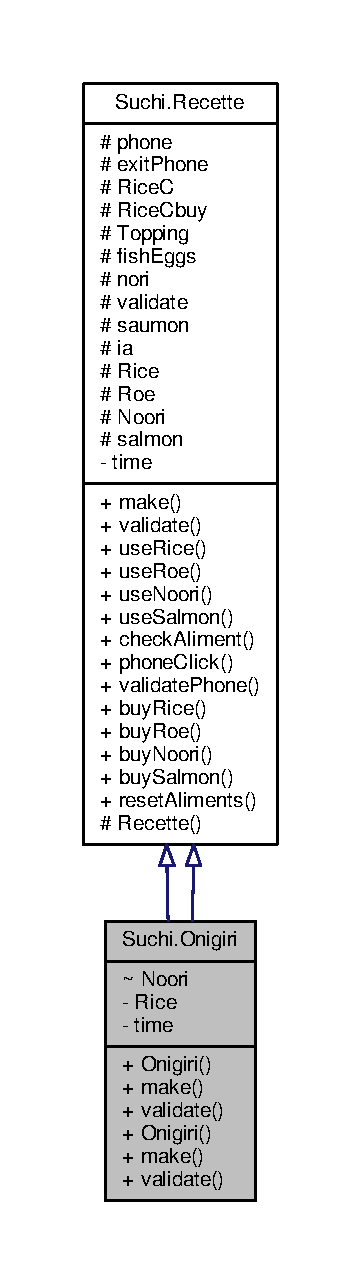
\includegraphics[height=550pt]{classSuchi_1_1Onigiri__inherit__graph}
\end{center}
\end{figure}


Graphe de collaboration de Suchi.\+Onigiri\+:\nopagebreak
\begin{figure}[H]
\begin{center}
\leavevmode
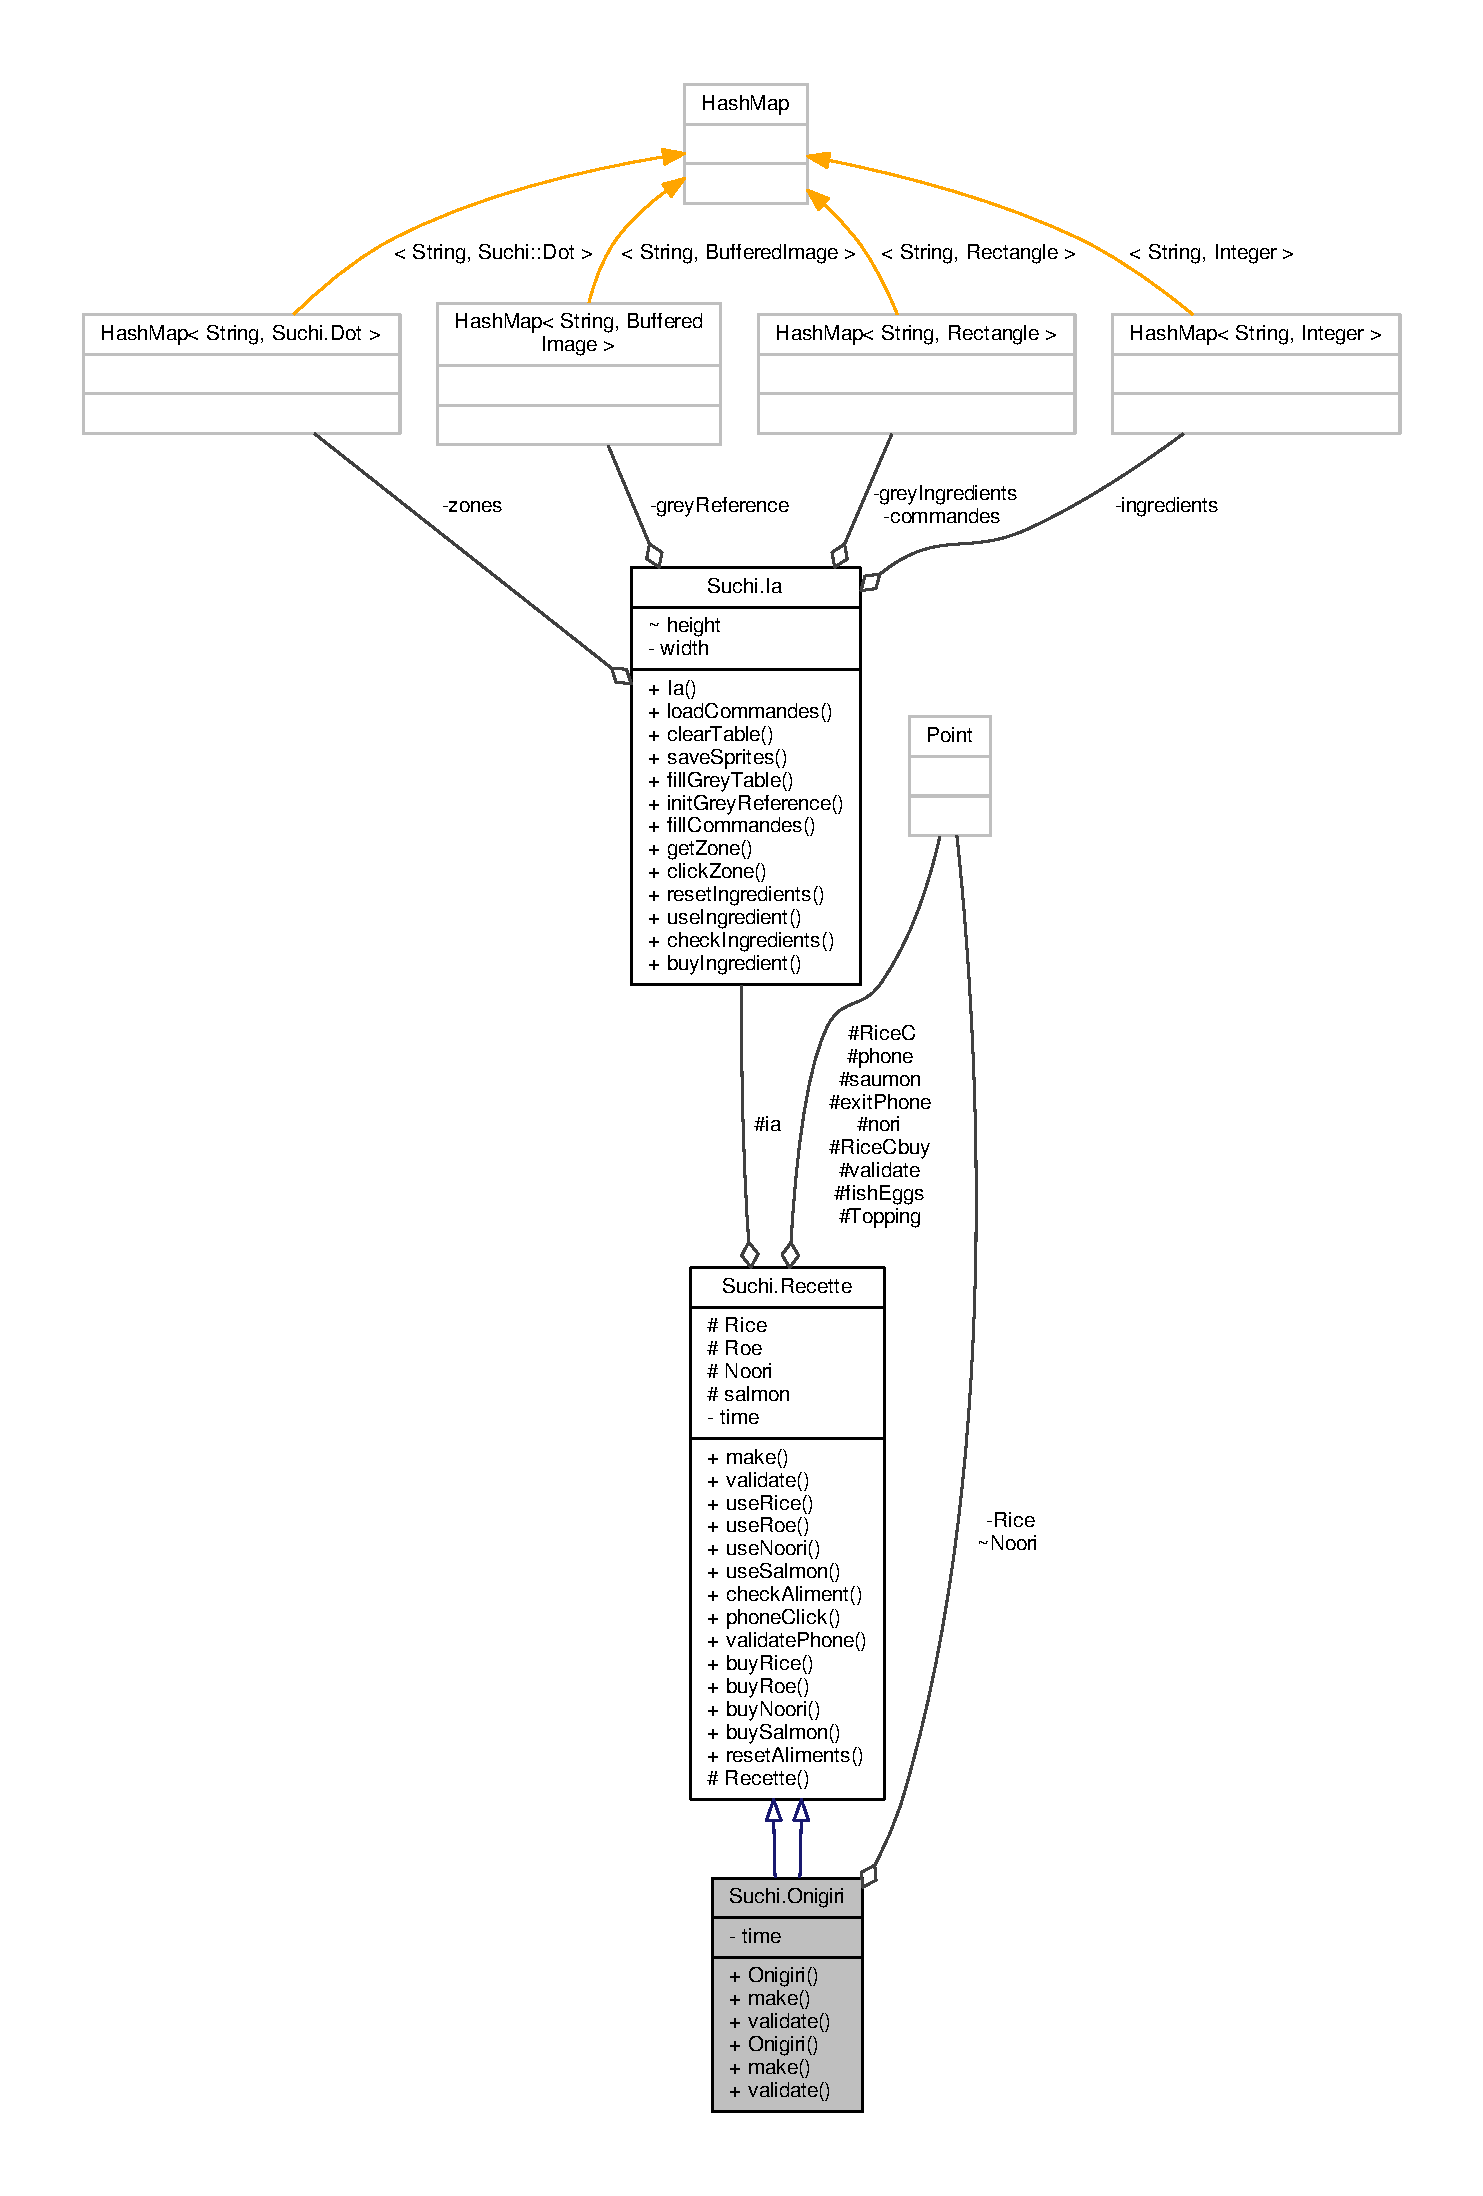
\includegraphics[width=350pt]{classSuchi_1_1Onigiri__coll__graph}
\end{center}
\end{figure}
\subsubsection*{Fonctions membres publiques}
\begin{DoxyCompactItemize}
\item 
\hyperlink{classSuchi_1_1Onigiri_a3f61f1822390fd76c39887e7f464f25b}{Onigiri} ()  throws Exception
\begin{DoxyCompactList}\small\item\em Constructeur. \end{DoxyCompactList}\item 
void \hyperlink{classSuchi_1_1Onigiri_a9be975ee57ccc08101af53611d4a3f88}{make} ()  throws Exception
\item 
void \hyperlink{classSuchi_1_1Onigiri_a82c4794ab8fd1c06a1fc8d2db572c042}{validate} ()  throws Exception
\item 
\hyperlink{classSuchi_1_1Onigiri_a3f61f1822390fd76c39887e7f464f25b}{Onigiri} ()  throws A\+W\+T\+Exception, Interrupted\+Exception
\item 
void \hyperlink{classSuchi_1_1Onigiri_a9be975ee57ccc08101af53611d4a3f88}{make} ()  throws A\+W\+T\+Exception
\item 
void \hyperlink{classSuchi_1_1Onigiri_a82c4794ab8fd1c06a1fc8d2db572c042}{validate} ()  throws A\+W\+T\+Exception 
\item 
void \hyperlink{classSuchi_1_1Recette_aa5204bd305d5029631ff4b8be9def83e}{use\+Rice} ()  throws A\+W\+T\+Exception, Interrupted\+Exception
\item 
void \hyperlink{classSuchi_1_1Recette_a500a2584148f1f08a1c7cdf7424e9a9c}{use\+Roe} ()  throws A\+W\+T\+Exception, Interrupted\+Exception
\item 
void \hyperlink{classSuchi_1_1Recette_a17d14fe05c28a44768d91e577e9bc511}{use\+Noori} ()  throws A\+W\+T\+Exception, Interrupted\+Exception
\item 
void \hyperlink{classSuchi_1_1Recette_a0fc2aa67439d0822762548c49cb29dec}{use\+Salmon} ()  throws A\+W\+T\+Exception, Interrupted\+Exception
\item 
void \hyperlink{classSuchi_1_1Recette_adc00873c980219a9a3fa7eddeaea3253}{check\+Aliment} ()  throws A\+W\+T\+Exception, Interrupted\+Exception
\item 
void \hyperlink{classSuchi_1_1Recette_a3e4c1e285cd28d0f2f2d364ea637c165}{phone\+Click} ()  throws A\+W\+T\+Exception, Interrupted\+Exception
\item 
void \hyperlink{classSuchi_1_1Recette_aae633102735c0f0a23f0aa84a0366fb3}{validate\+Phone} ()  throws A\+W\+T\+Exception
\item 
void \hyperlink{classSuchi_1_1Recette_a6e0c330317a6f65f2961d35f262362e7}{buy\+Rice} ()  throws A\+W\+T\+Exception, Interrupted\+Exception
\item 
void \hyperlink{classSuchi_1_1Recette_a019d29ed18bfa21dd4bf2ec681761fbf}{buy\+Roe} ()  throws A\+W\+T\+Exception, Interrupted\+Exception
\item 
void \hyperlink{classSuchi_1_1Recette_a31ee8b7bb1aeb396895509a5d5dea094}{buy\+Noori} ()  throws A\+W\+T\+Exception, Interrupted\+Exception
\item 
void \hyperlink{classSuchi_1_1Recette_aef0e38b7827110dbb4fd6a70777cddc1}{buy\+Salmon} ()  throws A\+W\+T\+Exception, Interrupted\+Exception
\end{DoxyCompactItemize}
\subsubsection*{Fonctions membres publiques statiques}
\begin{DoxyCompactItemize}
\item 
static void \hyperlink{classSuchi_1_1Recette_a99446c824f7bffe26c36e8433a4b18b3}{reset\+Aliments} ()
\end{DoxyCompactItemize}
\subsubsection*{Attributs protégés}
\begin{DoxyCompactItemize}
\item 
final Point \hyperlink{classSuchi_1_1Recette_a89465932bd180079526cfc1f8b8af456}{phone} = new Point (1030,620)
\item 
final Point \hyperlink{classSuchi_1_1Recette_ac7ff51ea8fa06174c38c52121b0ef767}{exit\+Phone} = new Point (1050,573)
\item 
final Point \hyperlink{classSuchi_1_1Recette_a36ec8dc3a30b3f1dba74d3aa354f9f11}{Rice\+C} = new Point (973,503)
\item 
final Point \hyperlink{classSuchi_1_1Recette_afc63b1a3fa7d921d606dc0c99d52cdf4}{Rice\+Cbuy} = new Point (976,487)
\item 
final Point \hyperlink{classSuchi_1_1Recette_a4810b2254c050209fba27757066668b3}{Topping} = new Point (978,470)
\item 
final Point \hyperlink{classSuchi_1_1Recette_a9d19fcc0de54e124694592bc35d97a1d}{fish\+Eggs} = new Point (979,472)
\item 
final Point \hyperlink{classSuchi_1_1Recette_ab86193f9fe4491190e232c4e7f93bed5}{nori} = new Point (929,469)
\item 
final Point \hyperlink{classSuchi_1_1Recette_aff16265c9b0b819091af71f64ef84be7}{validate} = new Point (900,500)
\item 
final Point \hyperlink{classSuchi_1_1Recette_a17aeabd21e3d4d55d7caae9a40bfc6a1}{saumon} = new Point (910,560)
\end{DoxyCompactItemize}
\subsubsection*{Attributs protégés statiques}
\begin{DoxyCompactItemize}
\item 
static \hyperlink{classSuchi_1_1Ia}{Ia} \hyperlink{classSuchi_1_1Recette_add9d95ee8955e02592b553c7e4b719a0}{ia}
\item 
static int \hyperlink{classSuchi_1_1Recette_acee61a97ab7dd56b74e2ef3decb5f3c4}{Roe} = 10
\item 
static int \hyperlink{classSuchi_1_1Recette_a2e9711072decb1bd2a64a4328e566d73}{salmon} = 5
\end{DoxyCompactItemize}
\subsubsection*{Attributs de paquetage}
\begin{DoxyCompactItemize}
\item 
Point \hyperlink{classSuchi_1_1Onigiri_a3a2c86dd6581e11512902fa76837f03a}{Noori}
\end{DoxyCompactItemize}
\subsubsection*{Attributs privés}
\begin{DoxyCompactItemize}
\item 
Point \hyperlink{classSuchi_1_1Onigiri_a564559717a3a63623d2b58163ce1ec85}{Rice}
\item 
final int \hyperlink{classSuchi_1_1Onigiri_a5b8da19f340d4f7e1909f002e12af16e}{time} = 500
\end{DoxyCompactItemize}


\subsubsection{Documentation des constructeurs et destructeur}
\hypertarget{classSuchi_1_1Onigiri_a3f61f1822390fd76c39887e7f464f25b}{}\index{Suchi\+::\+Onigiri@{Suchi\+::\+Onigiri}!Onigiri@{Onigiri}}
\index{Onigiri@{Onigiri}!Suchi\+::\+Onigiri@{Suchi\+::\+Onigiri}}
\paragraph[{Onigiri}]{\setlength{\rightskip}{0pt plus 5cm}Suchi.\+Onigiri.\+Onigiri (
\begin{DoxyParamCaption}
{}
\end{DoxyParamCaption}
) throws Exception}\label{classSuchi_1_1Onigiri_a3f61f1822390fd76c39887e7f464f25b}


Constructeur. 


\begin{DoxyExceptions}{Exceptions}
{\em Exception} & \\
\hline
\end{DoxyExceptions}
\hypertarget{classSuchi_1_1Onigiri_a3f61f1822390fd76c39887e7f464f25b}{}\index{Suchi\+::\+Onigiri@{Suchi\+::\+Onigiri}!Onigiri@{Onigiri}}
\index{Onigiri@{Onigiri}!Suchi\+::\+Onigiri@{Suchi\+::\+Onigiri}}
\paragraph[{Onigiri}]{\setlength{\rightskip}{0pt plus 5cm}Suchi.\+Onigiri.\+Onigiri (
\begin{DoxyParamCaption}
{}
\end{DoxyParamCaption}
) throws A\+W\+T\+Exception, Interrupted\+Exception}\label{classSuchi_1_1Onigiri_a3f61f1822390fd76c39887e7f464f25b}


\subsubsection{Documentation des fonctions membres}
\hypertarget{classSuchi_1_1Recette_a31ee8b7bb1aeb396895509a5d5dea094}{}\index{Suchi\+::\+Onigiri@{Suchi\+::\+Onigiri}!buy\+Noori@{buy\+Noori}}
\index{buy\+Noori@{buy\+Noori}!Suchi\+::\+Onigiri@{Suchi\+::\+Onigiri}}
\paragraph[{buy\+Noori}]{\setlength{\rightskip}{0pt plus 5cm}void Suchi.\+Recette.\+buy\+Noori (
\begin{DoxyParamCaption}
{}
\end{DoxyParamCaption}
) throws A\+W\+T\+Exception, Interrupted\+Exception\hspace{0.3cm}{\ttfamily [inherited]}}\label{classSuchi_1_1Recette_a31ee8b7bb1aeb396895509a5d5dea094}


Référencé par Suchi.\+Recette.\+check\+Aliment().

\hypertarget{classSuchi_1_1Recette_a6e0c330317a6f65f2961d35f262362e7}{}\index{Suchi\+::\+Onigiri@{Suchi\+::\+Onigiri}!buy\+Rice@{buy\+Rice}}
\index{buy\+Rice@{buy\+Rice}!Suchi\+::\+Onigiri@{Suchi\+::\+Onigiri}}
\paragraph[{buy\+Rice}]{\setlength{\rightskip}{0pt plus 5cm}void Suchi.\+Recette.\+buy\+Rice (
\begin{DoxyParamCaption}
{}
\end{DoxyParamCaption}
) throws A\+W\+T\+Exception, Interrupted\+Exception\hspace{0.3cm}{\ttfamily [inherited]}}\label{classSuchi_1_1Recette_a6e0c330317a6f65f2961d35f262362e7}


Référencé par Suchi.\+Recette.\+check\+Aliment().

\hypertarget{classSuchi_1_1Recette_a019d29ed18bfa21dd4bf2ec681761fbf}{}\index{Suchi\+::\+Onigiri@{Suchi\+::\+Onigiri}!buy\+Roe@{buy\+Roe}}
\index{buy\+Roe@{buy\+Roe}!Suchi\+::\+Onigiri@{Suchi\+::\+Onigiri}}
\paragraph[{buy\+Roe}]{\setlength{\rightskip}{0pt plus 5cm}void Suchi.\+Recette.\+buy\+Roe (
\begin{DoxyParamCaption}
{}
\end{DoxyParamCaption}
) throws A\+W\+T\+Exception, Interrupted\+Exception\hspace{0.3cm}{\ttfamily [inherited]}}\label{classSuchi_1_1Recette_a019d29ed18bfa21dd4bf2ec681761fbf}


Référencé par Suchi.\+Recette.\+check\+Aliment().

\hypertarget{classSuchi_1_1Recette_aef0e38b7827110dbb4fd6a70777cddc1}{}\index{Suchi\+::\+Onigiri@{Suchi\+::\+Onigiri}!buy\+Salmon@{buy\+Salmon}}
\index{buy\+Salmon@{buy\+Salmon}!Suchi\+::\+Onigiri@{Suchi\+::\+Onigiri}}
\paragraph[{buy\+Salmon}]{\setlength{\rightskip}{0pt plus 5cm}void Suchi.\+Recette.\+buy\+Salmon (
\begin{DoxyParamCaption}
{}
\end{DoxyParamCaption}
) throws A\+W\+T\+Exception, Interrupted\+Exception\hspace{0.3cm}{\ttfamily [inherited]}}\label{classSuchi_1_1Recette_aef0e38b7827110dbb4fd6a70777cddc1}


Référencé par Suchi.\+Recette.\+check\+Aliment().

\hypertarget{classSuchi_1_1Recette_adc00873c980219a9a3fa7eddeaea3253}{}\index{Suchi\+::\+Onigiri@{Suchi\+::\+Onigiri}!check\+Aliment@{check\+Aliment}}
\index{check\+Aliment@{check\+Aliment}!Suchi\+::\+Onigiri@{Suchi\+::\+Onigiri}}
\paragraph[{check\+Aliment}]{\setlength{\rightskip}{0pt plus 5cm}void Suchi.\+Recette.\+check\+Aliment (
\begin{DoxyParamCaption}
{}
\end{DoxyParamCaption}
) throws A\+W\+T\+Exception, Interrupted\+Exception\hspace{0.3cm}{\ttfamily [inherited]}}\label{classSuchi_1_1Recette_adc00873c980219a9a3fa7eddeaea3253}


Référencé par Suchi.\+Recette.\+use\+Noori(), Suchi.\+Recette.\+use\+Rice(), Suchi.\+Recette.\+use\+Roe(), et Suchi.\+Recette.\+use\+Salmon().

\hypertarget{classSuchi_1_1Onigiri_a9be975ee57ccc08101af53611d4a3f88}{}\index{Suchi\+::\+Onigiri@{Suchi\+::\+Onigiri}!make@{make}}
\index{make@{make}!Suchi\+::\+Onigiri@{Suchi\+::\+Onigiri}}
\paragraph[{make}]{\setlength{\rightskip}{0pt plus 5cm}void Suchi.\+Onigiri.\+make (
\begin{DoxyParamCaption}
{}
\end{DoxyParamCaption}
) throws Exception}\label{classSuchi_1_1Onigiri_a9be975ee57ccc08101af53611d4a3f88}


Référencé par Suchi.\+Onigiri.\+Onigiri().

\hypertarget{classSuchi_1_1Onigiri_a9be975ee57ccc08101af53611d4a3f88}{}\index{Suchi\+::\+Onigiri@{Suchi\+::\+Onigiri}!make@{make}}
\index{make@{make}!Suchi\+::\+Onigiri@{Suchi\+::\+Onigiri}}
\paragraph[{make}]{\setlength{\rightskip}{0pt plus 5cm}void Suchi.\+Onigiri.\+make (
\begin{DoxyParamCaption}
{}
\end{DoxyParamCaption}
) throws A\+W\+T\+Exception}\label{classSuchi_1_1Onigiri_a9be975ee57ccc08101af53611d4a3f88}
\hypertarget{classSuchi_1_1Recette_a3e4c1e285cd28d0f2f2d364ea637c165}{}\index{Suchi\+::\+Onigiri@{Suchi\+::\+Onigiri}!phone\+Click@{phone\+Click}}
\index{phone\+Click@{phone\+Click}!Suchi\+::\+Onigiri@{Suchi\+::\+Onigiri}}
\paragraph[{phone\+Click}]{\setlength{\rightskip}{0pt plus 5cm}void Suchi.\+Recette.\+phone\+Click (
\begin{DoxyParamCaption}
{}
\end{DoxyParamCaption}
) throws A\+W\+T\+Exception, Interrupted\+Exception\hspace{0.3cm}{\ttfamily [inherited]}}\label{classSuchi_1_1Recette_a3e4c1e285cd28d0f2f2d364ea637c165}


Référencé par Suchi.\+Recette.\+buy\+Noori(), Suchi.\+Recette.\+buy\+Rice(), Suchi.\+Recette.\+buy\+Roe(), et Suchi.\+Recette.\+buy\+Salmon().

\hypertarget{classSuchi_1_1Recette_a99446c824f7bffe26c36e8433a4b18b3}{}\index{Suchi\+::\+Onigiri@{Suchi\+::\+Onigiri}!reset\+Aliments@{reset\+Aliments}}
\index{reset\+Aliments@{reset\+Aliments}!Suchi\+::\+Onigiri@{Suchi\+::\+Onigiri}}
\paragraph[{reset\+Aliments}]{\setlength{\rightskip}{0pt plus 5cm}static void Suchi.\+Recette.\+reset\+Aliments (
\begin{DoxyParamCaption}
{}
\end{DoxyParamCaption}
)\hspace{0.3cm}{\ttfamily [static]}, {\ttfamily [inherited]}}\label{classSuchi_1_1Recette_a99446c824f7bffe26c36e8433a4b18b3}


Référencé par Suchi.\+Game.\+main().

\hypertarget{classSuchi_1_1Recette_a17d14fe05c28a44768d91e577e9bc511}{}\index{Suchi\+::\+Onigiri@{Suchi\+::\+Onigiri}!use\+Noori@{use\+Noori}}
\index{use\+Noori@{use\+Noori}!Suchi\+::\+Onigiri@{Suchi\+::\+Onigiri}}
\paragraph[{use\+Noori}]{\setlength{\rightskip}{0pt plus 5cm}void Suchi.\+Recette.\+use\+Noori (
\begin{DoxyParamCaption}
{}
\end{DoxyParamCaption}
) throws A\+W\+T\+Exception, Interrupted\+Exception\hspace{0.3cm}{\ttfamily [inherited]}}\label{classSuchi_1_1Recette_a17d14fe05c28a44768d91e577e9bc511}
\hypertarget{classSuchi_1_1Recette_aa5204bd305d5029631ff4b8be9def83e}{}\index{Suchi\+::\+Onigiri@{Suchi\+::\+Onigiri}!use\+Rice@{use\+Rice}}
\index{use\+Rice@{use\+Rice}!Suchi\+::\+Onigiri@{Suchi\+::\+Onigiri}}
\paragraph[{use\+Rice}]{\setlength{\rightskip}{0pt plus 5cm}void Suchi.\+Recette.\+use\+Rice (
\begin{DoxyParamCaption}
{}
\end{DoxyParamCaption}
) throws A\+W\+T\+Exception, Interrupted\+Exception\hspace{0.3cm}{\ttfamily [inherited]}}\label{classSuchi_1_1Recette_aa5204bd305d5029631ff4b8be9def83e}
\hypertarget{classSuchi_1_1Recette_a500a2584148f1f08a1c7cdf7424e9a9c}{}\index{Suchi\+::\+Onigiri@{Suchi\+::\+Onigiri}!use\+Roe@{use\+Roe}}
\index{use\+Roe@{use\+Roe}!Suchi\+::\+Onigiri@{Suchi\+::\+Onigiri}}
\paragraph[{use\+Roe}]{\setlength{\rightskip}{0pt plus 5cm}void Suchi.\+Recette.\+use\+Roe (
\begin{DoxyParamCaption}
{}
\end{DoxyParamCaption}
) throws A\+W\+T\+Exception, Interrupted\+Exception\hspace{0.3cm}{\ttfamily [inherited]}}\label{classSuchi_1_1Recette_a500a2584148f1f08a1c7cdf7424e9a9c}
\hypertarget{classSuchi_1_1Recette_a0fc2aa67439d0822762548c49cb29dec}{}\index{Suchi\+::\+Onigiri@{Suchi\+::\+Onigiri}!use\+Salmon@{use\+Salmon}}
\index{use\+Salmon@{use\+Salmon}!Suchi\+::\+Onigiri@{Suchi\+::\+Onigiri}}
\paragraph[{use\+Salmon}]{\setlength{\rightskip}{0pt plus 5cm}void Suchi.\+Recette.\+use\+Salmon (
\begin{DoxyParamCaption}
{}
\end{DoxyParamCaption}
) throws A\+W\+T\+Exception, Interrupted\+Exception\hspace{0.3cm}{\ttfamily [inherited]}}\label{classSuchi_1_1Recette_a0fc2aa67439d0822762548c49cb29dec}
\hypertarget{classSuchi_1_1Onigiri_a82c4794ab8fd1c06a1fc8d2db572c042}{}\index{Suchi\+::\+Onigiri@{Suchi\+::\+Onigiri}!validate@{validate}}
\index{validate@{validate}!Suchi\+::\+Onigiri@{Suchi\+::\+Onigiri}}
\paragraph[{validate}]{\setlength{\rightskip}{0pt plus 5cm}void Suchi.\+Onigiri.\+validate (
\begin{DoxyParamCaption}
{}
\end{DoxyParamCaption}
) throws Exception}\label{classSuchi_1_1Onigiri_a82c4794ab8fd1c06a1fc8d2db572c042}


Référencé par Suchi.\+Onigiri.\+Onigiri().

\hypertarget{classSuchi_1_1Onigiri_a82c4794ab8fd1c06a1fc8d2db572c042}{}\index{Suchi\+::\+Onigiri@{Suchi\+::\+Onigiri}!validate@{validate}}
\index{validate@{validate}!Suchi\+::\+Onigiri@{Suchi\+::\+Onigiri}}
\paragraph[{validate}]{\setlength{\rightskip}{0pt plus 5cm}void Suchi.\+Onigiri.\+validate (
\begin{DoxyParamCaption}
{}
\end{DoxyParamCaption}
) throws A\+W\+T\+Exception}\label{classSuchi_1_1Onigiri_a82c4794ab8fd1c06a1fc8d2db572c042}
\hypertarget{classSuchi_1_1Recette_aae633102735c0f0a23f0aa84a0366fb3}{}\index{Suchi\+::\+Onigiri@{Suchi\+::\+Onigiri}!validate\+Phone@{validate\+Phone}}
\index{validate\+Phone@{validate\+Phone}!Suchi\+::\+Onigiri@{Suchi\+::\+Onigiri}}
\paragraph[{validate\+Phone}]{\setlength{\rightskip}{0pt plus 5cm}void Suchi.\+Recette.\+validate\+Phone (
\begin{DoxyParamCaption}
{}
\end{DoxyParamCaption}
) throws A\+W\+T\+Exception\hspace{0.3cm}{\ttfamily [inherited]}}\label{classSuchi_1_1Recette_aae633102735c0f0a23f0aa84a0366fb3}


Référencé par Suchi.\+Recette.\+buy\+Noori(), Suchi.\+Recette.\+buy\+Rice(), Suchi.\+Recette.\+buy\+Roe(), et Suchi.\+Recette.\+buy\+Salmon().



\subsubsection{Documentation des données membres}
\hypertarget{classSuchi_1_1Recette_ac7ff51ea8fa06174c38c52121b0ef767}{}\index{Suchi\+::\+Onigiri@{Suchi\+::\+Onigiri}!exit\+Phone@{exit\+Phone}}
\index{exit\+Phone@{exit\+Phone}!Suchi\+::\+Onigiri@{Suchi\+::\+Onigiri}}
\paragraph[{exit\+Phone}]{\setlength{\rightskip}{0pt plus 5cm}final Point Suchi.\+Recette.\+exit\+Phone = new Point (1050,573)\hspace{0.3cm}{\ttfamily [protected]}, {\ttfamily [inherited]}}\label{classSuchi_1_1Recette_ac7ff51ea8fa06174c38c52121b0ef767}
\hypertarget{classSuchi_1_1Recette_a9d19fcc0de54e124694592bc35d97a1d}{}\index{Suchi\+::\+Onigiri@{Suchi\+::\+Onigiri}!fish\+Eggs@{fish\+Eggs}}
\index{fish\+Eggs@{fish\+Eggs}!Suchi\+::\+Onigiri@{Suchi\+::\+Onigiri}}
\paragraph[{fish\+Eggs}]{\setlength{\rightskip}{0pt plus 5cm}final Point Suchi.\+Recette.\+fish\+Eggs = new Point (979,472)\hspace{0.3cm}{\ttfamily [protected]}, {\ttfamily [inherited]}}\label{classSuchi_1_1Recette_a9d19fcc0de54e124694592bc35d97a1d}
\hypertarget{classSuchi_1_1Recette_add9d95ee8955e02592b553c7e4b719a0}{}\index{Suchi\+::\+Onigiri@{Suchi\+::\+Onigiri}!ia@{ia}}
\index{ia@{ia}!Suchi\+::\+Onigiri@{Suchi\+::\+Onigiri}}
\paragraph[{ia}]{\setlength{\rightskip}{0pt plus 5cm}{\bf Ia} Suchi.\+Recette.\+ia\hspace{0.3cm}{\ttfamily [static]}, {\ttfamily [protected]}, {\ttfamily [inherited]}}\label{classSuchi_1_1Recette_add9d95ee8955e02592b553c7e4b719a0}


Référencé par Suchi.\+Salmon.\+make(), Suchi.\+California.\+make(), Suchi.\+Onigiri.\+make(), Suchi.\+Maki.\+make(), Suchi.\+Shrimp\+Sh.\+make(), Suchi.\+Salmon.\+validate(), Suchi.\+Onigiri.\+validate(), Suchi.\+California.\+validate(), Suchi.\+Maki.\+validate(), et Suchi.\+Shrimp\+Sh.\+validate().

\hypertarget{classSuchi_1_1Onigiri_a3a2c86dd6581e11512902fa76837f03a}{}\index{Suchi\+::\+Onigiri@{Suchi\+::\+Onigiri}!Noori@{Noori}}
\index{Noori@{Noori}!Suchi\+::\+Onigiri@{Suchi\+::\+Onigiri}}
\paragraph[{Noori}]{\setlength{\rightskip}{0pt plus 5cm}Point Suchi.\+Onigiri.\+Noori\hspace{0.3cm}{\ttfamily [package]}}\label{classSuchi_1_1Onigiri_a3a2c86dd6581e11512902fa76837f03a}
\hypertarget{classSuchi_1_1Recette_ab86193f9fe4491190e232c4e7f93bed5}{}\index{Suchi\+::\+Onigiri@{Suchi\+::\+Onigiri}!nori@{nori}}
\index{nori@{nori}!Suchi\+::\+Onigiri@{Suchi\+::\+Onigiri}}
\paragraph[{nori}]{\setlength{\rightskip}{0pt plus 5cm}final Point Suchi.\+Recette.\+nori = new Point (929,469)\hspace{0.3cm}{\ttfamily [protected]}, {\ttfamily [inherited]}}\label{classSuchi_1_1Recette_ab86193f9fe4491190e232c4e7f93bed5}
\hypertarget{classSuchi_1_1Recette_a89465932bd180079526cfc1f8b8af456}{}\index{Suchi\+::\+Onigiri@{Suchi\+::\+Onigiri}!phone@{phone}}
\index{phone@{phone}!Suchi\+::\+Onigiri@{Suchi\+::\+Onigiri}}
\paragraph[{phone}]{\setlength{\rightskip}{0pt plus 5cm}final Point Suchi.\+Recette.\+phone = new Point (1030,620)\hspace{0.3cm}{\ttfamily [protected]}, {\ttfamily [inherited]}}\label{classSuchi_1_1Recette_a89465932bd180079526cfc1f8b8af456}
\hypertarget{classSuchi_1_1Onigiri_a564559717a3a63623d2b58163ce1ec85}{}\index{Suchi\+::\+Onigiri@{Suchi\+::\+Onigiri}!Rice@{Rice}}
\index{Rice@{Rice}!Suchi\+::\+Onigiri@{Suchi\+::\+Onigiri}}
\paragraph[{Rice}]{\setlength{\rightskip}{0pt plus 5cm}Point Suchi.\+Onigiri.\+Rice\hspace{0.3cm}{\ttfamily [private]}}\label{classSuchi_1_1Onigiri_a564559717a3a63623d2b58163ce1ec85}
\hypertarget{classSuchi_1_1Recette_a36ec8dc3a30b3f1dba74d3aa354f9f11}{}\index{Suchi\+::\+Onigiri@{Suchi\+::\+Onigiri}!Rice\+C@{Rice\+C}}
\index{Rice\+C@{Rice\+C}!Suchi\+::\+Onigiri@{Suchi\+::\+Onigiri}}
\paragraph[{Rice\+C}]{\setlength{\rightskip}{0pt plus 5cm}final Point Suchi.\+Recette.\+Rice\+C = new Point (973,503)\hspace{0.3cm}{\ttfamily [protected]}, {\ttfamily [inherited]}}\label{classSuchi_1_1Recette_a36ec8dc3a30b3f1dba74d3aa354f9f11}
\hypertarget{classSuchi_1_1Recette_afc63b1a3fa7d921d606dc0c99d52cdf4}{}\index{Suchi\+::\+Onigiri@{Suchi\+::\+Onigiri}!Rice\+Cbuy@{Rice\+Cbuy}}
\index{Rice\+Cbuy@{Rice\+Cbuy}!Suchi\+::\+Onigiri@{Suchi\+::\+Onigiri}}
\paragraph[{Rice\+Cbuy}]{\setlength{\rightskip}{0pt plus 5cm}final Point Suchi.\+Recette.\+Rice\+Cbuy = new Point (976,487)\hspace{0.3cm}{\ttfamily [protected]}, {\ttfamily [inherited]}}\label{classSuchi_1_1Recette_afc63b1a3fa7d921d606dc0c99d52cdf4}
\hypertarget{classSuchi_1_1Recette_acee61a97ab7dd56b74e2ef3decb5f3c4}{}\index{Suchi\+::\+Onigiri@{Suchi\+::\+Onigiri}!Roe@{Roe}}
\index{Roe@{Roe}!Suchi\+::\+Onigiri@{Suchi\+::\+Onigiri}}
\paragraph[{Roe}]{\setlength{\rightskip}{0pt plus 5cm}int Suchi.\+Recette.\+Roe = 10\hspace{0.3cm}{\ttfamily [static]}, {\ttfamily [protected]}, {\ttfamily [inherited]}}\label{classSuchi_1_1Recette_acee61a97ab7dd56b74e2ef3decb5f3c4}
\hypertarget{classSuchi_1_1Recette_a2e9711072decb1bd2a64a4328e566d73}{}\index{Suchi\+::\+Onigiri@{Suchi\+::\+Onigiri}!salmon@{salmon}}
\index{salmon@{salmon}!Suchi\+::\+Onigiri@{Suchi\+::\+Onigiri}}
\paragraph[{salmon}]{\setlength{\rightskip}{0pt plus 5cm}int Suchi.\+Recette.\+salmon = 5\hspace{0.3cm}{\ttfamily [static]}, {\ttfamily [protected]}, {\ttfamily [inherited]}}\label{classSuchi_1_1Recette_a2e9711072decb1bd2a64a4328e566d73}
\hypertarget{classSuchi_1_1Recette_a17aeabd21e3d4d55d7caae9a40bfc6a1}{}\index{Suchi\+::\+Onigiri@{Suchi\+::\+Onigiri}!saumon@{saumon}}
\index{saumon@{saumon}!Suchi\+::\+Onigiri@{Suchi\+::\+Onigiri}}
\paragraph[{saumon}]{\setlength{\rightskip}{0pt plus 5cm}final Point Suchi.\+Recette.\+saumon = new Point (910,560)\hspace{0.3cm}{\ttfamily [protected]}, {\ttfamily [inherited]}}\label{classSuchi_1_1Recette_a17aeabd21e3d4d55d7caae9a40bfc6a1}
\hypertarget{classSuchi_1_1Onigiri_a5b8da19f340d4f7e1909f002e12af16e}{}\index{Suchi\+::\+Onigiri@{Suchi\+::\+Onigiri}!time@{time}}
\index{time@{time}!Suchi\+::\+Onigiri@{Suchi\+::\+Onigiri}}
\paragraph[{time}]{\setlength{\rightskip}{0pt plus 5cm}final int Suchi.\+Onigiri.\+time = 500\hspace{0.3cm}{\ttfamily [private]}}\label{classSuchi_1_1Onigiri_a5b8da19f340d4f7e1909f002e12af16e}
\hypertarget{classSuchi_1_1Recette_a4810b2254c050209fba27757066668b3}{}\index{Suchi\+::\+Onigiri@{Suchi\+::\+Onigiri}!Topping@{Topping}}
\index{Topping@{Topping}!Suchi\+::\+Onigiri@{Suchi\+::\+Onigiri}}
\paragraph[{Topping}]{\setlength{\rightskip}{0pt plus 5cm}final Point Suchi.\+Recette.\+Topping = new Point (978,470)\hspace{0.3cm}{\ttfamily [protected]}, {\ttfamily [inherited]}}\label{classSuchi_1_1Recette_a4810b2254c050209fba27757066668b3}
\hypertarget{classSuchi_1_1Recette_aff16265c9b0b819091af71f64ef84be7}{}\index{Suchi\+::\+Onigiri@{Suchi\+::\+Onigiri}!validate@{validate}}
\index{validate@{validate}!Suchi\+::\+Onigiri@{Suchi\+::\+Onigiri}}
\paragraph[{validate}]{\setlength{\rightskip}{0pt plus 5cm}final Point Suchi.\+Recette.\+validate = new Point (900,500)\hspace{0.3cm}{\ttfamily [protected]}, {\ttfamily [inherited]}}\label{classSuchi_1_1Recette_aff16265c9b0b819091af71f64ef84be7}


La documentation de cette classe a été générée à partir du fichier suivant \+:\begin{DoxyCompactItemize}
\item 
\hyperlink{BotSofRetapage_2src_2Suchi_2Onigiri_8java}{Bot\+Sof\+Retapage/src/\+Suchi/\+Onigiri.\+java}\end{DoxyCompactItemize}

\hypertarget{classSuchi_1_1Prog}{}\subsection{Référence de la classe Suchi.\+Prog}
\label{classSuchi_1_1Prog}\index{Suchi.\+Prog@{Suchi.\+Prog}}


Graphe de collaboration de Suchi.\+Prog\+:\nopagebreak
\begin{figure}[H]
\begin{center}
\leavevmode
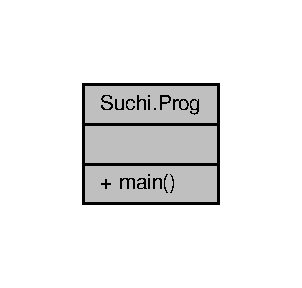
\includegraphics[width=145pt]{classSuchi_1_1Prog__coll__graph}
\end{center}
\end{figure}
\subsubsection*{Fonctions membres publiques statiques}
\begin{DoxyCompactItemize}
\item 
static void \hyperlink{classSuchi_1_1Prog_a2e5347233c00b37ee0131b08fad64b44}{main} (String\mbox{[}$\,$\mbox{]}args)  throws Exception 
\end{DoxyCompactItemize}


\subsubsection{Documentation des fonctions membres}
\hypertarget{classSuchi_1_1Prog_a2e5347233c00b37ee0131b08fad64b44}{}\index{Suchi\+::\+Prog@{Suchi\+::\+Prog}!main@{main}}
\index{main@{main}!Suchi\+::\+Prog@{Suchi\+::\+Prog}}
\paragraph[{main}]{\setlength{\rightskip}{0pt plus 5cm}static void Suchi.\+Prog.\+main (
\begin{DoxyParamCaption}
\item[{String\mbox{[}$\,$\mbox{]}}]{args}
\end{DoxyParamCaption}
) throws Exception\hspace{0.3cm}{\ttfamily [static]}}\label{classSuchi_1_1Prog_a2e5347233c00b37ee0131b08fad64b44}


La documentation de cette classe a été générée à partir du fichier suivant \+:\begin{DoxyCompactItemize}
\item 
\hyperlink{BotSuchis_2TestSuchis_2Suchi_2Prog_8java}{Bot\+Suchis/\+Test\+Suchis/\+Suchi/\+Prog.\+java}\end{DoxyCompactItemize}

\hypertarget{classProg}{\section{Référence de la classe Prog}
\label{classProg}\index{Prog@{Prog}}
}
\subsection*{Fonctions membres publiques statiques}
\begin{DoxyCompactItemize}
\item 
\hypertarget{classProg_a6a74608deae3c0733cc81cd5338dd002}{static void {\bfseries main} (String\mbox{[}$\,$\mbox{]}args)  throws Exception }\label{classProg_a6a74608deae3c0733cc81cd5338dd002}

\end{DoxyCompactItemize}


La documentation de cette classe a été générée à partir du fichier suivant \+:\begin{DoxyCompactItemize}
\item 
Prog.\+java\end{DoxyCompactItemize}

\hypertarget{classSushis_1_1src_1_1Prog}{}\subsection{Référence de la classe Sushis.\+src.\+Prog}
\label{classSushis_1_1src_1_1Prog}\index{Sushis.\+src.\+Prog@{Sushis.\+src.\+Prog}}


Graphe de collaboration de Sushis.\+src.\+Prog\+:\nopagebreak
\begin{figure}[H]
\begin{center}
\leavevmode
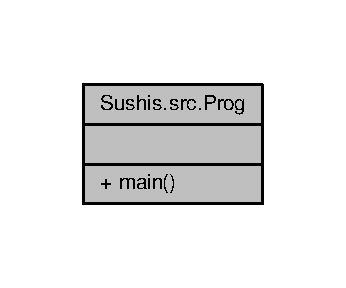
\includegraphics[width=166pt]{classSushis_1_1src_1_1Prog__coll__graph}
\end{center}
\end{figure}
\subsubsection*{Fonctions membres publiques statiques}
\begin{DoxyCompactItemize}
\item 
static void \hyperlink{classSushis_1_1src_1_1Prog_abe985e2a4e4603a2c7e2420b071972a8}{main} (String\mbox{[}$\,$\mbox{]} args)  throws Exception 
\end{DoxyCompactItemize}


\subsubsection{Documentation des fonctions membres}
\hypertarget{classSushis_1_1src_1_1Prog_abe985e2a4e4603a2c7e2420b071972a8}{}\index{Sushis\+::src\+::\+Prog@{Sushis\+::src\+::\+Prog}!main@{main}}
\index{main@{main}!Sushis\+::src\+::\+Prog@{Sushis\+::src\+::\+Prog}}
\paragraph[{main}]{\setlength{\rightskip}{0pt plus 5cm}static void Sushis.\+src.\+Prog.\+main (
\begin{DoxyParamCaption}
\item[{String\mbox{[}$\,$\mbox{]}}]{args}
\end{DoxyParamCaption}
) throws Exception\hspace{0.3cm}{\ttfamily [static]}}\label{classSushis_1_1src_1_1Prog_abe985e2a4e4603a2c7e2420b071972a8}


La documentation de cette classe a été générée à partir du fichier suivant \+:\begin{DoxyCompactItemize}
\item 
\hyperlink{projet_2Sushis_2src_2Prog_8java}{projet/\+Sushis/src/\+Prog.\+java}\end{DoxyCompactItemize}

\hypertarget{classmain_1_1Prog}{}\subsection{Référence de la classe main.\+Prog}
\label{classmain_1_1Prog}\index{main.\+Prog@{main.\+Prog}}


Graphe de collaboration de main.\+Prog\+:\nopagebreak
\begin{figure}[H]
\begin{center}
\leavevmode
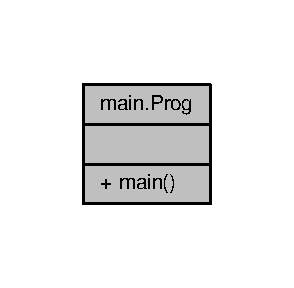
\includegraphics[width=141pt]{classmain_1_1Prog__coll__graph}
\end{center}
\end{figure}
\subsubsection*{Fonctions membres publiques statiques}
\begin{DoxyCompactItemize}
\item 
static void \hyperlink{classmain_1_1Prog_a4a2c61e449f1214e0a9cde28b6f3309c}{main} (String\mbox{[}$\,$\mbox{]} args)  throws Exception 
\end{DoxyCompactItemize}


\subsubsection{Documentation des fonctions membres}
\hypertarget{classmain_1_1Prog_a4a2c61e449f1214e0a9cde28b6f3309c}{}\index{main\+::\+Prog@{main\+::\+Prog}!main@{main}}
\index{main@{main}!main\+::\+Prog@{main\+::\+Prog}}
\paragraph[{main}]{\setlength{\rightskip}{0pt plus 5cm}static void main.\+Prog.\+main (
\begin{DoxyParamCaption}
\item[{String\mbox{[}$\,$\mbox{]}}]{args}
\end{DoxyParamCaption}
) throws Exception\hspace{0.3cm}{\ttfamily [static]}}\label{classmain_1_1Prog_a4a2c61e449f1214e0a9cde28b6f3309c}


La documentation de cette classe a été générée à partir du fichier suivant \+:\begin{DoxyCompactItemize}
\item 
\hyperlink{main_2Prog_8java}{main/\+Prog.\+java}\end{DoxyCompactItemize}

\hypertarget{classSushis_1_1src_1_1ReadZone}{}\subsection{Référence de la classe Sushis.\+src.\+Read\+Zone}
\label{classSushis_1_1src_1_1ReadZone}\index{Sushis.\+src.\+Read\+Zone@{Sushis.\+src.\+Read\+Zone}}


Graphe de collaboration de Sushis.\+src.\+Read\+Zone\+:\nopagebreak
\begin{figure}[H]
\begin{center}
\leavevmode
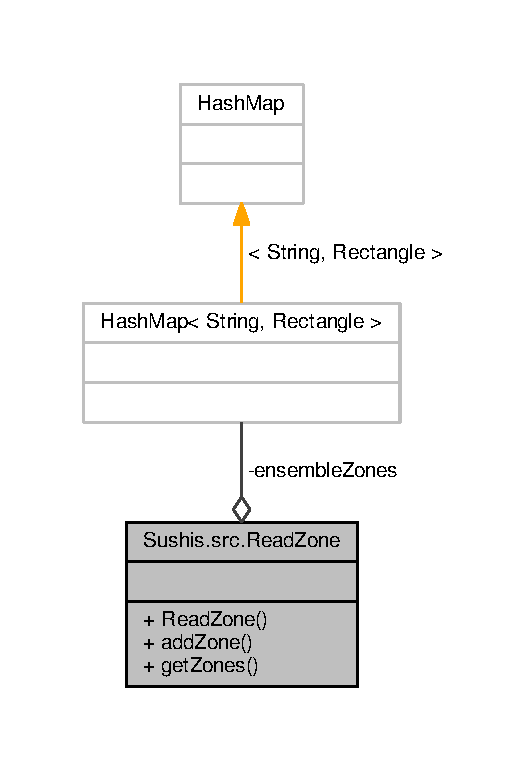
\includegraphics[width=253pt]{classSushis_1_1src_1_1ReadZone__coll__graph}
\end{center}
\end{figure}
\subsubsection*{Fonctions membres publiques}
\begin{DoxyCompactItemize}
\item 
\hyperlink{classSushis_1_1src_1_1ReadZone_a1fd767e508cbc3ce6bbdef61d3ba9b8f}{Read\+Zone} ()
\item 
void \hyperlink{classSushis_1_1src_1_1ReadZone_a142e2eb0d5890f48f92825f7deaabc12}{add\+Zone} (String nom, Point origin, int width, int height)
\item 
Hash\+Map$<$ String, Rectangle $>$ \hyperlink{classSushis_1_1src_1_1ReadZone_abaef7d55c09d629dddc128a4a17d7d5d}{get\+Zones} ()
\end{DoxyCompactItemize}
\subsubsection*{Attributs privés}
\begin{DoxyCompactItemize}
\item 
Hash\+Map$<$ String, Rectangle $>$ \hyperlink{classSushis_1_1src_1_1ReadZone_a588f6513d5899c3ae9bb3b0154487cba}{ensemble\+Zones}
\end{DoxyCompactItemize}


\subsubsection{Documentation des constructeurs et destructeur}
\hypertarget{classSushis_1_1src_1_1ReadZone_a1fd767e508cbc3ce6bbdef61d3ba9b8f}{}\index{Sushis\+::src\+::\+Read\+Zone@{Sushis\+::src\+::\+Read\+Zone}!Read\+Zone@{Read\+Zone}}
\index{Read\+Zone@{Read\+Zone}!Sushis\+::src\+::\+Read\+Zone@{Sushis\+::src\+::\+Read\+Zone}}
\paragraph[{Read\+Zone}]{\setlength{\rightskip}{0pt plus 5cm}Sushis.\+src.\+Read\+Zone.\+Read\+Zone (
\begin{DoxyParamCaption}
{}
\end{DoxyParamCaption}
)}\label{classSushis_1_1src_1_1ReadZone_a1fd767e508cbc3ce6bbdef61d3ba9b8f}


\subsubsection{Documentation des fonctions membres}
\hypertarget{classSushis_1_1src_1_1ReadZone_a142e2eb0d5890f48f92825f7deaabc12}{}\index{Sushis\+::src\+::\+Read\+Zone@{Sushis\+::src\+::\+Read\+Zone}!add\+Zone@{add\+Zone}}
\index{add\+Zone@{add\+Zone}!Sushis\+::src\+::\+Read\+Zone@{Sushis\+::src\+::\+Read\+Zone}}
\paragraph[{add\+Zone}]{\setlength{\rightskip}{0pt plus 5cm}void Sushis.\+src.\+Read\+Zone.\+add\+Zone (
\begin{DoxyParamCaption}
\item[{String}]{nom, }
\item[{Point}]{origin, }
\item[{int}]{width, }
\item[{int}]{height}
\end{DoxyParamCaption}
)}\label{classSushis_1_1src_1_1ReadZone_a142e2eb0d5890f48f92825f7deaabc12}


Référencé par Sushis.\+src.\+I\+A.\+I\+A().

\hypertarget{classSushis_1_1src_1_1ReadZone_abaef7d55c09d629dddc128a4a17d7d5d}{}\index{Sushis\+::src\+::\+Read\+Zone@{Sushis\+::src\+::\+Read\+Zone}!get\+Zones@{get\+Zones}}
\index{get\+Zones@{get\+Zones}!Sushis\+::src\+::\+Read\+Zone@{Sushis\+::src\+::\+Read\+Zone}}
\paragraph[{get\+Zones}]{\setlength{\rightskip}{0pt plus 5cm}Hash\+Map$<$String, Rectangle$>$ Sushis.\+src.\+Read\+Zone.\+get\+Zones (
\begin{DoxyParamCaption}
{}
\end{DoxyParamCaption}
)}\label{classSushis_1_1src_1_1ReadZone_abaef7d55c09d629dddc128a4a17d7d5d}


Référencé par Sushis.\+src.\+I\+A.\+load\+Sprites(), et Sushis.\+src.\+I\+A.\+save\+Sprites().



\subsubsection{Documentation des données membres}
\hypertarget{classSushis_1_1src_1_1ReadZone_a588f6513d5899c3ae9bb3b0154487cba}{}\index{Sushis\+::src\+::\+Read\+Zone@{Sushis\+::src\+::\+Read\+Zone}!ensemble\+Zones@{ensemble\+Zones}}
\index{ensemble\+Zones@{ensemble\+Zones}!Sushis\+::src\+::\+Read\+Zone@{Sushis\+::src\+::\+Read\+Zone}}
\paragraph[{ensemble\+Zones}]{\setlength{\rightskip}{0pt plus 5cm}Hash\+Map$<$String, Rectangle$>$ Sushis.\+src.\+Read\+Zone.\+ensemble\+Zones\hspace{0.3cm}{\ttfamily [private]}}\label{classSushis_1_1src_1_1ReadZone_a588f6513d5899c3ae9bb3b0154487cba}


Référencé par Sushis.\+src.\+Read\+Zone.\+get\+Zones().



La documentation de cette classe a été générée à partir du fichier suivant \+:\begin{DoxyCompactItemize}
\item 
\hyperlink{projet_2Sushis_2src_2ReadZone_8java}{projet/\+Sushis/src/\+Read\+Zone.\+java}\end{DoxyCompactItemize}

\hypertarget{classReadZone}{}\subsection{Référence de la classe Read\+Zone}
\label{classReadZone}\index{Read\+Zone@{Read\+Zone}}


Graphe de collaboration de Read\+Zone\+:\nopagebreak
\begin{figure}[H]
\begin{center}
\leavevmode
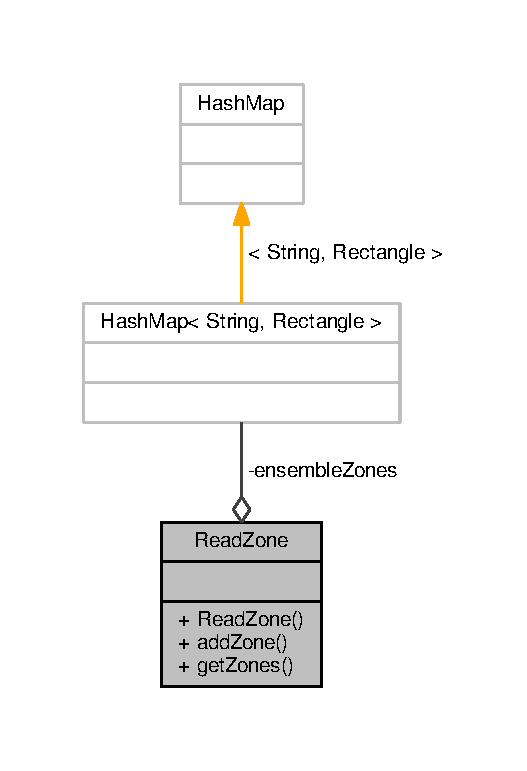
\includegraphics[width=253pt]{classReadZone__coll__graph}
\end{center}
\end{figure}
\subsubsection*{Fonctions membres publiques}
\begin{DoxyCompactItemize}
\item 
\hyperlink{classReadZone_a6250748967f86ba603ac7466573afda0}{Read\+Zone} ()
\item 
void \hyperlink{classReadZone_abeba8d3981f584dedc5dcb815e11e8a8}{add\+Zone} (String nom, \hyperlink{classDot}{Dot} origin, double width, double height)
\item 
Hash\+Map$<$ String, Rectangle $>$ \hyperlink{classReadZone_a03ccc10559e83a0d923442a0956f24a1}{get\+Zones} ()
\end{DoxyCompactItemize}
\subsubsection*{Attributs privés}
\begin{DoxyCompactItemize}
\item 
Hash\+Map$<$ String, Rectangle $>$ \hyperlink{classReadZone_aef32e4cb03f8f591c736911be6d8bd5c}{ensemble\+Zones}
\end{DoxyCompactItemize}


\subsubsection{Documentation des constructeurs et destructeur}
\hypertarget{classReadZone_a6250748967f86ba603ac7466573afda0}{}\index{Read\+Zone@{Read\+Zone}!Read\+Zone@{Read\+Zone}}
\index{Read\+Zone@{Read\+Zone}!Read\+Zone@{Read\+Zone}}
\paragraph[{Read\+Zone}]{\setlength{\rightskip}{0pt plus 5cm}Read\+Zone.\+Read\+Zone (
\begin{DoxyParamCaption}
{}
\end{DoxyParamCaption}
)}\label{classReadZone_a6250748967f86ba603ac7466573afda0}


\subsubsection{Documentation des fonctions membres}
\hypertarget{classReadZone_abeba8d3981f584dedc5dcb815e11e8a8}{}\index{Read\+Zone@{Read\+Zone}!add\+Zone@{add\+Zone}}
\index{add\+Zone@{add\+Zone}!Read\+Zone@{Read\+Zone}}
\paragraph[{add\+Zone}]{\setlength{\rightskip}{0pt plus 5cm}void Read\+Zone.\+add\+Zone (
\begin{DoxyParamCaption}
\item[{String}]{nom, }
\item[{{\bf Dot}}]{origin, }
\item[{double}]{width, }
\item[{double}]{height}
\end{DoxyParamCaption}
)}\label{classReadZone_abeba8d3981f584dedc5dcb815e11e8a8}


Référencé par I\+A.\+I\+A().

\hypertarget{classReadZone_a03ccc10559e83a0d923442a0956f24a1}{}\index{Read\+Zone@{Read\+Zone}!get\+Zones@{get\+Zones}}
\index{get\+Zones@{get\+Zones}!Read\+Zone@{Read\+Zone}}
\paragraph[{get\+Zones}]{\setlength{\rightskip}{0pt plus 5cm}Hash\+Map$<$String, Rectangle$>$ Read\+Zone.\+get\+Zones (
\begin{DoxyParamCaption}
{}
\end{DoxyParamCaption}
)}\label{classReadZone_a03ccc10559e83a0d923442a0956f24a1}


Référencé par I\+A.\+load\+Sprites(), et I\+A.\+save\+Sprites().



\subsubsection{Documentation des données membres}
\hypertarget{classReadZone_aef32e4cb03f8f591c736911be6d8bd5c}{}\index{Read\+Zone@{Read\+Zone}!ensemble\+Zones@{ensemble\+Zones}}
\index{ensemble\+Zones@{ensemble\+Zones}!Read\+Zone@{Read\+Zone}}
\paragraph[{ensemble\+Zones}]{\setlength{\rightskip}{0pt plus 5cm}Hash\+Map$<$String, Rectangle$>$ Read\+Zone.\+ensemble\+Zones\hspace{0.3cm}{\ttfamily [private]}}\label{classReadZone_aef32e4cb03f8f591c736911be6d8bd5c}


Référencé par get\+Zones().



La documentation de cette classe a été générée à partir du fichier suivant \+:\begin{DoxyCompactItemize}
\item 
\hyperlink{oldCode_2ReadZone_8java}{old\+Code/\+Read\+Zone.\+java}\end{DoxyCompactItemize}

\hypertarget{classmain_1_1ReadZone}{}\subsection{Référence de la classe main.\+Read\+Zone}
\label{classmain_1_1ReadZone}\index{main.\+Read\+Zone@{main.\+Read\+Zone}}


Graphe de collaboration de main.\+Read\+Zone\+:\nopagebreak
\begin{figure}[H]
\begin{center}
\leavevmode
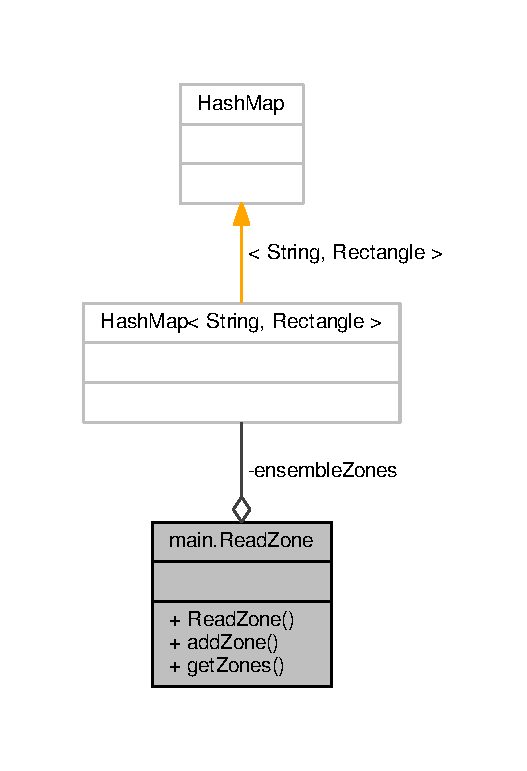
\includegraphics[width=253pt]{classmain_1_1ReadZone__coll__graph}
\end{center}
\end{figure}
\subsubsection*{Fonctions membres publiques}
\begin{DoxyCompactItemize}
\item 
\hyperlink{classmain_1_1ReadZone_a4a154c5e019dbeb1c6e57fd9a6ec9a2b}{Read\+Zone} ()
\item 
void \hyperlink{classmain_1_1ReadZone_a7e15ad634ac892871bf7207b7e10cffe}{add\+Zone} (String nom, \hyperlink{classmain_1_1Dot}{Dot} origin, int width, int height)
\item 
Hash\+Map$<$ String, Rectangle $>$ \hyperlink{classmain_1_1ReadZone_a060b745d9dac448790df108839cc670f}{get\+Zones} ()
\end{DoxyCompactItemize}
\subsubsection*{Attributs privés}
\begin{DoxyCompactItemize}
\item 
Hash\+Map$<$ String, Rectangle $>$ \hyperlink{classmain_1_1ReadZone_afdcc575ea21ea8cca2b387b6b60d018e}{ensemble\+Zones}
\end{DoxyCompactItemize}


\subsubsection{Documentation des constructeurs et destructeur}
\hypertarget{classmain_1_1ReadZone_a4a154c5e019dbeb1c6e57fd9a6ec9a2b}{}\index{main\+::\+Read\+Zone@{main\+::\+Read\+Zone}!Read\+Zone@{Read\+Zone}}
\index{Read\+Zone@{Read\+Zone}!main\+::\+Read\+Zone@{main\+::\+Read\+Zone}}
\paragraph[{Read\+Zone}]{\setlength{\rightskip}{0pt plus 5cm}main.\+Read\+Zone.\+Read\+Zone (
\begin{DoxyParamCaption}
{}
\end{DoxyParamCaption}
)}\label{classmain_1_1ReadZone_a4a154c5e019dbeb1c6e57fd9a6ec9a2b}


\subsubsection{Documentation des fonctions membres}
\hypertarget{classmain_1_1ReadZone_a7e15ad634ac892871bf7207b7e10cffe}{}\index{main\+::\+Read\+Zone@{main\+::\+Read\+Zone}!add\+Zone@{add\+Zone}}
\index{add\+Zone@{add\+Zone}!main\+::\+Read\+Zone@{main\+::\+Read\+Zone}}
\paragraph[{add\+Zone}]{\setlength{\rightskip}{0pt plus 5cm}void main.\+Read\+Zone.\+add\+Zone (
\begin{DoxyParamCaption}
\item[{String}]{nom, }
\item[{{\bf Dot}}]{origin, }
\item[{int}]{width, }
\item[{int}]{height}
\end{DoxyParamCaption}
)}\label{classmain_1_1ReadZone_a7e15ad634ac892871bf7207b7e10cffe}


Référencé par main.\+I\+A.\+I\+A().

\hypertarget{classmain_1_1ReadZone_a060b745d9dac448790df108839cc670f}{}\index{main\+::\+Read\+Zone@{main\+::\+Read\+Zone}!get\+Zones@{get\+Zones}}
\index{get\+Zones@{get\+Zones}!main\+::\+Read\+Zone@{main\+::\+Read\+Zone}}
\paragraph[{get\+Zones}]{\setlength{\rightskip}{0pt plus 5cm}Hash\+Map$<$String, Rectangle$>$ main.\+Read\+Zone.\+get\+Zones (
\begin{DoxyParamCaption}
{}
\end{DoxyParamCaption}
)}\label{classmain_1_1ReadZone_a060b745d9dac448790df108839cc670f}


Référencé par main.\+I\+A.\+load\+Sprites(), et main.\+I\+A.\+save\+Sprites().



\subsubsection{Documentation des données membres}
\hypertarget{classmain_1_1ReadZone_afdcc575ea21ea8cca2b387b6b60d018e}{}\index{main\+::\+Read\+Zone@{main\+::\+Read\+Zone}!ensemble\+Zones@{ensemble\+Zones}}
\index{ensemble\+Zones@{ensemble\+Zones}!main\+::\+Read\+Zone@{main\+::\+Read\+Zone}}
\paragraph[{ensemble\+Zones}]{\setlength{\rightskip}{0pt plus 5cm}Hash\+Map$<$String, Rectangle$>$ main.\+Read\+Zone.\+ensemble\+Zones\hspace{0.3cm}{\ttfamily [private]}}\label{classmain_1_1ReadZone_afdcc575ea21ea8cca2b387b6b60d018e}


Référencé par main.\+Read\+Zone.\+get\+Zones().



La documentation de cette classe a été générée à partir du fichier suivant \+:\begin{DoxyCompactItemize}
\item 
\hyperlink{main_2ReadZone_8java}{main/\+Read\+Zone.\+java}\end{DoxyCompactItemize}

\hypertarget{classTestSushi_1_1src_1_1Suchi_1_1Recette}{}\subsection{Référence de la classe Test\+Sushi.\+src.\+Suchi.\+Recette}
\label{classTestSushi_1_1src_1_1Suchi_1_1Recette}\index{Test\+Sushi.\+src.\+Suchi.\+Recette@{Test\+Sushi.\+src.\+Suchi.\+Recette}}


Graphe d\textquotesingle{}héritage de Test\+Sushi.\+src.\+Suchi.\+Recette\+:\nopagebreak
\begin{figure}[H]
\begin{center}
\leavevmode
\includegraphics[width=350pt]{classTestSushi_1_1src_1_1Suchi_1_1Recette__inherit__graph}
\end{center}
\end{figure}


Graphe de collaboration de Test\+Sushi.\+src.\+Suchi.\+Recette\+:\nopagebreak
\begin{figure}[H]
\begin{center}
\leavevmode
\includegraphics[height=550pt]{classTestSushi_1_1src_1_1Suchi_1_1Recette__coll__graph}
\end{center}
\end{figure}
\subsubsection*{Fonctions membres publiques}
\begin{DoxyCompactItemize}
\item 
void \hyperlink{classTestSushi_1_1src_1_1Suchi_1_1Recette_a2d78a4575d1295e34210e2f77c01f3f3}{use\+Rice} ()  throws A\+W\+T\+Exception, Interrupted\+Exception
\item 
void \hyperlink{classTestSushi_1_1src_1_1Suchi_1_1Recette_a8967a205e78d02ef7c30fd435fbaa0af}{use\+Roe} ()  throws A\+W\+T\+Exception, Interrupted\+Exception
\item 
void \hyperlink{classTestSushi_1_1src_1_1Suchi_1_1Recette_a10bfe3c71750c84144203a7aa2c341ee}{use\+Noori} ()  throws A\+W\+T\+Exception, Interrupted\+Exception
\item 
void \hyperlink{classTestSushi_1_1src_1_1Suchi_1_1Recette_a87cd9338767df0e5db88e6005f1da984}{use\+Salmon} ()  throws A\+W\+T\+Exception, Interrupted\+Exception
\item 
void \hyperlink{classTestSushi_1_1src_1_1Suchi_1_1Recette_ab2c165554830ba84a392765621604d44}{use\+Shrimp} ()  throws A\+W\+T\+Exception, Interrupted\+Exception
\item 
void \hyperlink{classTestSushi_1_1src_1_1Suchi_1_1Recette_a83f9f5fb6bfe2691974a5e35386e7b8a}{check\+Aliment} ()  throws A\+W\+T\+Exception, Interrupted\+Exception
\item 
void \hyperlink{classTestSushi_1_1src_1_1Suchi_1_1Recette_ad94006ea131c2379a14c50eec870b69b}{phone\+Click} ()  throws A\+W\+T\+Exception, Interrupted\+Exception
\item 
void \hyperlink{classTestSushi_1_1src_1_1Suchi_1_1Recette_a33f0912e1212b01ea1b3787bed28f0fe}{validate\+Phone} ()  throws A\+W\+T\+Exception
\item 
void \hyperlink{classTestSushi_1_1src_1_1Suchi_1_1Recette_aa0fc4c335f6ab3f905f63a16902a6379}{buy\+Rice} ()  throws A\+W\+T\+Exception, Interrupted\+Exception
\item 
void \hyperlink{classTestSushi_1_1src_1_1Suchi_1_1Recette_ad874ba9daf68328d6b65b09e6f16003e}{buy\+Roe} ()  throws A\+W\+T\+Exception, Interrupted\+Exception
\item 
void \hyperlink{classTestSushi_1_1src_1_1Suchi_1_1Recette_a5602befaaef8858b75c131e50f7cf91d}{buy\+Noori} ()  throws A\+W\+T\+Exception, Interrupted\+Exception
\item 
void \hyperlink{classTestSushi_1_1src_1_1Suchi_1_1Recette_a64cf6254490e04e9e8031d564a4a0ea3}{buy\+Salmon} ()  throws A\+W\+T\+Exception, Interrupted\+Exception
\item 
void \hyperlink{classTestSushi_1_1src_1_1Suchi_1_1Recette_a0d15202c729b3c6b2bb699de4137d551}{buy\+Shrimp} ()  throws A\+W\+T\+Exception, Interrupted\+Exception
\end{DoxyCompactItemize}
\subsubsection*{Fonctions membres publiques statiques}
\begin{DoxyCompactItemize}
\item 
static void \hyperlink{classTestSushi_1_1src_1_1Suchi_1_1Recette_aef7faa1aea5f8aeb869c612af16e4e62}{reset\+Aliments} ()
\end{DoxyCompactItemize}
\subsubsection*{Attributs protégés}
\begin{DoxyCompactItemize}
\item 
final String \hyperlink{classTestSushi_1_1src_1_1Suchi_1_1Recette_a14892e43d9ed57350effdf3ed1bddb8a}{egggris} = \char`\"{}sprites/egg\+Gris.\+png\char`\"{}
\item 
final String \hyperlink{classTestSushi_1_1src_1_1Suchi_1_1Recette_a774959efa525787a162778df37770b7c}{norigris} = \char`\"{}sprites/nori\+Gris.\+png\char`\"{}
\item 
final String \hyperlink{classTestSushi_1_1src_1_1Suchi_1_1Recette_aea59cc2a5f6bc21ec36690a5bf1eb38c}{saumongris} =\char`\"{}sprites/saumon\+Gris.\+png\char`\"{}
\item 
final String \hyperlink{classTestSushi_1_1src_1_1Suchi_1_1Recette_a616939eea675e05aa6d7ec62fd90f461}{ricegris} = \char`\"{}sprites/rice\+Gris.\+png\char`\"{}
\item 
final String \hyperlink{classTestSushi_1_1src_1_1Suchi_1_1Recette_ac1b1b9b91dba95a9d0df2f6e59f04a59}{shrimp\+Gris} = \char`\"{}sprites/shrimp\+Gris.\+png\char`\"{}
\item 
final Point \hyperlink{classTestSushi_1_1src_1_1Suchi_1_1Recette_a45e48b1a85957813f1a747df04923b08}{phone} = new Point (1030,620)
\item 
final Point \hyperlink{classTestSushi_1_1src_1_1Suchi_1_1Recette_aecc6de3619013f1fb5f506c1e4e9ad7b}{exit\+Phone} = new Point (1050,573)
\item 
final Point \hyperlink{classTestSushi_1_1src_1_1Suchi_1_1Recette_ab502e1d023a0bd3fadfc714e1babc728}{Rice\+C} = new Point (973,503)
\item 
final Point \hyperlink{classTestSushi_1_1src_1_1Suchi_1_1Recette_a890dce3bb5d54a700fa7bebc2496e931}{Rice\+Cbuy} = new Point (976,487)
\item 
final Point \hyperlink{classTestSushi_1_1src_1_1Suchi_1_1Recette_ab7575f64998864f6b053859c18380f58}{Topping} = new Point (978,470)
\item 
final Point \hyperlink{classTestSushi_1_1src_1_1Suchi_1_1Recette_a2f5cec48c186dc52c3d990df66f3a8cf}{fish\+Eggs} = new Point (979,472)
\item 
final Point \hyperlink{classTestSushi_1_1src_1_1Suchi_1_1Recette_a4f3e62b4ab32fcc5d8b6875996f47618}{nori} = new Point (929,469)
\item 
final Point \hyperlink{classTestSushi_1_1src_1_1Suchi_1_1Recette_a9c491e7f09a444817e433e54923e6bca}{validate} = new Point (900,500)
\item 
final Point \hyperlink{classTestSushi_1_1src_1_1Suchi_1_1Recette_a855a7ed217eec3565619156fa6cd4214}{saumon} = new Point (910,560)
\item 
final Point \hyperlink{classTestSushi_1_1src_1_1Suchi_1_1Recette_a69faeadec2c0d475bbd77c3b7eeaada7}{shrimp\+Coord} = new Point (907,386)
\item 
final int \hyperlink{classTestSushi_1_1src_1_1Suchi_1_1Recette_a2c78759553661a7e4b01d4ac1212ec6c}{time} = 150
\item 
final int \hyperlink{classTestSushi_1_1src_1_1Suchi_1_1Recette_a0d95a4a68ee0d423b6815b296f3304b2}{phone\+Time} = 50
\item 
final int \hyperlink{classTestSushi_1_1src_1_1Suchi_1_1Recette_a7db8ec6383e36487bc7ca0490edd0b4a}{time\+Tapis} = 650
\end{DoxyCompactItemize}
\subsubsection*{Attributs protégés statiques}
\begin{DoxyCompactItemize}
\item 
static int \hyperlink{classTestSushi_1_1src_1_1Suchi_1_1Recette_a7c4936908dc847a0fc257304562c6c78}{Rice} = 10
\item 
static int \hyperlink{classTestSushi_1_1src_1_1Suchi_1_1Recette_ab4ceb10875120aaae2ade481b6088c6d}{Roe} = 10
\item 
static int \hyperlink{classTestSushi_1_1src_1_1Suchi_1_1Recette_a3ee55c3ec1870fa9abf2921e39a219bb}{Noori} = 10
\item 
static int \hyperlink{classTestSushi_1_1src_1_1Suchi_1_1Recette_a726a712fe936ef2a96982e00d21c49c0}{salmon} = 5
\item 
static int \hyperlink{classTestSushi_1_1src_1_1Suchi_1_1Recette_a07fa939a0df1b7ff45a9d4aa77498e8e}{shrimp} = 5
\end{DoxyCompactItemize}


\subsubsection{Documentation des fonctions membres}
\hypertarget{classTestSushi_1_1src_1_1Suchi_1_1Recette_a5602befaaef8858b75c131e50f7cf91d}{}\index{Test\+Sushi\+::src\+::\+Suchi\+::\+Recette@{Test\+Sushi\+::src\+::\+Suchi\+::\+Recette}!buy\+Noori@{buy\+Noori}}
\index{buy\+Noori@{buy\+Noori}!Test\+Sushi\+::src\+::\+Suchi\+::\+Recette@{Test\+Sushi\+::src\+::\+Suchi\+::\+Recette}}
\paragraph[{buy\+Noori}]{\setlength{\rightskip}{0pt plus 5cm}void Test\+Sushi.\+src.\+Suchi.\+Recette.\+buy\+Noori (
\begin{DoxyParamCaption}
{}
\end{DoxyParamCaption}
) throws A\+W\+T\+Exception, Interrupted\+Exception}\label{classTestSushi_1_1src_1_1Suchi_1_1Recette_a5602befaaef8858b75c131e50f7cf91d}

\begin{DoxyExceptions}{Exceptions}
{\em A\+W\+T\+Exception} & \\
\hline
{\em Interrupted\+Exception} & \\
\hline
\end{DoxyExceptions}


Référencé par Test\+Sushi.\+src.\+Suchi.\+Recette.\+check\+Aliment().

\hypertarget{classTestSushi_1_1src_1_1Suchi_1_1Recette_aa0fc4c335f6ab3f905f63a16902a6379}{}\index{Test\+Sushi\+::src\+::\+Suchi\+::\+Recette@{Test\+Sushi\+::src\+::\+Suchi\+::\+Recette}!buy\+Rice@{buy\+Rice}}
\index{buy\+Rice@{buy\+Rice}!Test\+Sushi\+::src\+::\+Suchi\+::\+Recette@{Test\+Sushi\+::src\+::\+Suchi\+::\+Recette}}
\paragraph[{buy\+Rice}]{\setlength{\rightskip}{0pt plus 5cm}void Test\+Sushi.\+src.\+Suchi.\+Recette.\+buy\+Rice (
\begin{DoxyParamCaption}
{}
\end{DoxyParamCaption}
) throws A\+W\+T\+Exception, Interrupted\+Exception}\label{classTestSushi_1_1src_1_1Suchi_1_1Recette_aa0fc4c335f6ab3f905f63a16902a6379}

\begin{DoxyExceptions}{Exceptions}
{\em A\+W\+T\+Exception} & \\
\hline
{\em Interrupted\+Exception} & \\
\hline
\end{DoxyExceptions}


Référencé par Test\+Sushi.\+src.\+Suchi.\+Recette.\+check\+Aliment().

\hypertarget{classTestSushi_1_1src_1_1Suchi_1_1Recette_ad874ba9daf68328d6b65b09e6f16003e}{}\index{Test\+Sushi\+::src\+::\+Suchi\+::\+Recette@{Test\+Sushi\+::src\+::\+Suchi\+::\+Recette}!buy\+Roe@{buy\+Roe}}
\index{buy\+Roe@{buy\+Roe}!Test\+Sushi\+::src\+::\+Suchi\+::\+Recette@{Test\+Sushi\+::src\+::\+Suchi\+::\+Recette}}
\paragraph[{buy\+Roe}]{\setlength{\rightskip}{0pt plus 5cm}void Test\+Sushi.\+src.\+Suchi.\+Recette.\+buy\+Roe (
\begin{DoxyParamCaption}
{}
\end{DoxyParamCaption}
) throws A\+W\+T\+Exception, Interrupted\+Exception}\label{classTestSushi_1_1src_1_1Suchi_1_1Recette_ad874ba9daf68328d6b65b09e6f16003e}

\begin{DoxyExceptions}{Exceptions}
{\em A\+W\+T\+Exception} & \\
\hline
{\em Interrupted\+Exception} & \\
\hline
\end{DoxyExceptions}


Référencé par Test\+Sushi.\+src.\+Suchi.\+Recette.\+check\+Aliment().

\hypertarget{classTestSushi_1_1src_1_1Suchi_1_1Recette_a64cf6254490e04e9e8031d564a4a0ea3}{}\index{Test\+Sushi\+::src\+::\+Suchi\+::\+Recette@{Test\+Sushi\+::src\+::\+Suchi\+::\+Recette}!buy\+Salmon@{buy\+Salmon}}
\index{buy\+Salmon@{buy\+Salmon}!Test\+Sushi\+::src\+::\+Suchi\+::\+Recette@{Test\+Sushi\+::src\+::\+Suchi\+::\+Recette}}
\paragraph[{buy\+Salmon}]{\setlength{\rightskip}{0pt plus 5cm}void Test\+Sushi.\+src.\+Suchi.\+Recette.\+buy\+Salmon (
\begin{DoxyParamCaption}
{}
\end{DoxyParamCaption}
) throws A\+W\+T\+Exception, Interrupted\+Exception}\label{classTestSushi_1_1src_1_1Suchi_1_1Recette_a64cf6254490e04e9e8031d564a4a0ea3}

\begin{DoxyExceptions}{Exceptions}
{\em A\+W\+T\+Exception} & \\
\hline
{\em Interrupted\+Exception} & \\
\hline
\end{DoxyExceptions}


Référencé par Test\+Sushi.\+src.\+Suchi.\+Recette.\+check\+Aliment().

\hypertarget{classTestSushi_1_1src_1_1Suchi_1_1Recette_a0d15202c729b3c6b2bb699de4137d551}{}\index{Test\+Sushi\+::src\+::\+Suchi\+::\+Recette@{Test\+Sushi\+::src\+::\+Suchi\+::\+Recette}!buy\+Shrimp@{buy\+Shrimp}}
\index{buy\+Shrimp@{buy\+Shrimp}!Test\+Sushi\+::src\+::\+Suchi\+::\+Recette@{Test\+Sushi\+::src\+::\+Suchi\+::\+Recette}}
\paragraph[{buy\+Shrimp}]{\setlength{\rightskip}{0pt plus 5cm}void Test\+Sushi.\+src.\+Suchi.\+Recette.\+buy\+Shrimp (
\begin{DoxyParamCaption}
{}
\end{DoxyParamCaption}
) throws A\+W\+T\+Exception, Interrupted\+Exception}\label{classTestSushi_1_1src_1_1Suchi_1_1Recette_a0d15202c729b3c6b2bb699de4137d551}

\begin{DoxyExceptions}{Exceptions}
{\em A\+W\+T\+Exception} & \\
\hline
{\em Interrupted\+Exception} & \\
\hline
\end{DoxyExceptions}


Référencé par Test\+Sushi.\+src.\+Suchi.\+Recette.\+check\+Aliment().

\hypertarget{classTestSushi_1_1src_1_1Suchi_1_1Recette_a83f9f5fb6bfe2691974a5e35386e7b8a}{}\index{Test\+Sushi\+::src\+::\+Suchi\+::\+Recette@{Test\+Sushi\+::src\+::\+Suchi\+::\+Recette}!check\+Aliment@{check\+Aliment}}
\index{check\+Aliment@{check\+Aliment}!Test\+Sushi\+::src\+::\+Suchi\+::\+Recette@{Test\+Sushi\+::src\+::\+Suchi\+::\+Recette}}
\paragraph[{check\+Aliment}]{\setlength{\rightskip}{0pt plus 5cm}void Test\+Sushi.\+src.\+Suchi.\+Recette.\+check\+Aliment (
\begin{DoxyParamCaption}
{}
\end{DoxyParamCaption}
) throws A\+W\+T\+Exception, Interrupted\+Exception}\label{classTestSushi_1_1src_1_1Suchi_1_1Recette_a83f9f5fb6bfe2691974a5e35386e7b8a}

\begin{DoxyExceptions}{Exceptions}
{\em A\+W\+T\+Exception} & \\
\hline
{\em Interrupted\+Exception} & \\
\hline
\end{DoxyExceptions}


Référencé par Test\+Sushi.\+src.\+Suchi.\+Recette.\+use\+Noori(), Test\+Sushi.\+src.\+Suchi.\+Recette.\+use\+Rice(), Test\+Sushi.\+src.\+Suchi.\+Recette.\+use\+Roe(), Test\+Sushi.\+src.\+Suchi.\+Recette.\+use\+Salmon(), et Test\+Sushi.\+src.\+Suchi.\+Recette.\+use\+Shrimp().

\hypertarget{classTestSushi_1_1src_1_1Suchi_1_1Recette_ad94006ea131c2379a14c50eec870b69b}{}\index{Test\+Sushi\+::src\+::\+Suchi\+::\+Recette@{Test\+Sushi\+::src\+::\+Suchi\+::\+Recette}!phone\+Click@{phone\+Click}}
\index{phone\+Click@{phone\+Click}!Test\+Sushi\+::src\+::\+Suchi\+::\+Recette@{Test\+Sushi\+::src\+::\+Suchi\+::\+Recette}}
\paragraph[{phone\+Click}]{\setlength{\rightskip}{0pt plus 5cm}void Test\+Sushi.\+src.\+Suchi.\+Recette.\+phone\+Click (
\begin{DoxyParamCaption}
{}
\end{DoxyParamCaption}
) throws A\+W\+T\+Exception, Interrupted\+Exception}\label{classTestSushi_1_1src_1_1Suchi_1_1Recette_ad94006ea131c2379a14c50eec870b69b}

\begin{DoxyExceptions}{Exceptions}
{\em A\+W\+T\+Exception} & \\
\hline
{\em Interrupted\+Exception} & \\
\hline
\end{DoxyExceptions}


Référencé par Test\+Sushi.\+src.\+Suchi.\+Recette.\+buy\+Noori(), Test\+Sushi.\+src.\+Suchi.\+Recette.\+buy\+Rice(), Test\+Sushi.\+src.\+Suchi.\+Recette.\+buy\+Roe(), Test\+Sushi.\+src.\+Suchi.\+Recette.\+buy\+Salmon(), et Test\+Sushi.\+src.\+Suchi.\+Recette.\+buy\+Shrimp().

\hypertarget{classTestSushi_1_1src_1_1Suchi_1_1Recette_aef7faa1aea5f8aeb869c612af16e4e62}{}\index{Test\+Sushi\+::src\+::\+Suchi\+::\+Recette@{Test\+Sushi\+::src\+::\+Suchi\+::\+Recette}!reset\+Aliments@{reset\+Aliments}}
\index{reset\+Aliments@{reset\+Aliments}!Test\+Sushi\+::src\+::\+Suchi\+::\+Recette@{Test\+Sushi\+::src\+::\+Suchi\+::\+Recette}}
\paragraph[{reset\+Aliments}]{\setlength{\rightskip}{0pt plus 5cm}static void Test\+Sushi.\+src.\+Suchi.\+Recette.\+reset\+Aliments (
\begin{DoxyParamCaption}
{}
\end{DoxyParamCaption}
)\hspace{0.3cm}{\ttfamily [static]}}\label{classTestSushi_1_1src_1_1Suchi_1_1Recette_aef7faa1aea5f8aeb869c612af16e4e62}


Référencé par Test\+Sushi.\+src.\+Suchi.\+Game.\+start\+Level2(), et Test\+Sushi.\+src.\+Suchi.\+Game.\+start\+Level3().

\hypertarget{classTestSushi_1_1src_1_1Suchi_1_1Recette_a10bfe3c71750c84144203a7aa2c341ee}{}\index{Test\+Sushi\+::src\+::\+Suchi\+::\+Recette@{Test\+Sushi\+::src\+::\+Suchi\+::\+Recette}!use\+Noori@{use\+Noori}}
\index{use\+Noori@{use\+Noori}!Test\+Sushi\+::src\+::\+Suchi\+::\+Recette@{Test\+Sushi\+::src\+::\+Suchi\+::\+Recette}}
\paragraph[{use\+Noori}]{\setlength{\rightskip}{0pt plus 5cm}void Test\+Sushi.\+src.\+Suchi.\+Recette.\+use\+Noori (
\begin{DoxyParamCaption}
{}
\end{DoxyParamCaption}
) throws A\+W\+T\+Exception, Interrupted\+Exception}\label{classTestSushi_1_1src_1_1Suchi_1_1Recette_a10bfe3c71750c84144203a7aa2c341ee}

\begin{DoxyExceptions}{Exceptions}
{\em A\+W\+T\+Exception} & \\
\hline
{\em Interrupted\+Exception} & \\
\hline
\end{DoxyExceptions}
\hypertarget{classTestSushi_1_1src_1_1Suchi_1_1Recette_a2d78a4575d1295e34210e2f77c01f3f3}{}\index{Test\+Sushi\+::src\+::\+Suchi\+::\+Recette@{Test\+Sushi\+::src\+::\+Suchi\+::\+Recette}!use\+Rice@{use\+Rice}}
\index{use\+Rice@{use\+Rice}!Test\+Sushi\+::src\+::\+Suchi\+::\+Recette@{Test\+Sushi\+::src\+::\+Suchi\+::\+Recette}}
\paragraph[{use\+Rice}]{\setlength{\rightskip}{0pt plus 5cm}void Test\+Sushi.\+src.\+Suchi.\+Recette.\+use\+Rice (
\begin{DoxyParamCaption}
{}
\end{DoxyParamCaption}
) throws A\+W\+T\+Exception, Interrupted\+Exception}\label{classTestSushi_1_1src_1_1Suchi_1_1Recette_a2d78a4575d1295e34210e2f77c01f3f3}

\begin{DoxyExceptions}{Exceptions}
{\em A\+W\+T\+Exception} & \\
\hline
{\em Interrupted\+Exception} & \\
\hline
\end{DoxyExceptions}
\hypertarget{classTestSushi_1_1src_1_1Suchi_1_1Recette_a8967a205e78d02ef7c30fd435fbaa0af}{}\index{Test\+Sushi\+::src\+::\+Suchi\+::\+Recette@{Test\+Sushi\+::src\+::\+Suchi\+::\+Recette}!use\+Roe@{use\+Roe}}
\index{use\+Roe@{use\+Roe}!Test\+Sushi\+::src\+::\+Suchi\+::\+Recette@{Test\+Sushi\+::src\+::\+Suchi\+::\+Recette}}
\paragraph[{use\+Roe}]{\setlength{\rightskip}{0pt plus 5cm}void Test\+Sushi.\+src.\+Suchi.\+Recette.\+use\+Roe (
\begin{DoxyParamCaption}
{}
\end{DoxyParamCaption}
) throws A\+W\+T\+Exception, Interrupted\+Exception}\label{classTestSushi_1_1src_1_1Suchi_1_1Recette_a8967a205e78d02ef7c30fd435fbaa0af}

\begin{DoxyExceptions}{Exceptions}
{\em A\+W\+T\+Exception} & \\
\hline
{\em Interrupted\+Exception} & \\
\hline
\end{DoxyExceptions}
\hypertarget{classTestSushi_1_1src_1_1Suchi_1_1Recette_a87cd9338767df0e5db88e6005f1da984}{}\index{Test\+Sushi\+::src\+::\+Suchi\+::\+Recette@{Test\+Sushi\+::src\+::\+Suchi\+::\+Recette}!use\+Salmon@{use\+Salmon}}
\index{use\+Salmon@{use\+Salmon}!Test\+Sushi\+::src\+::\+Suchi\+::\+Recette@{Test\+Sushi\+::src\+::\+Suchi\+::\+Recette}}
\paragraph[{use\+Salmon}]{\setlength{\rightskip}{0pt plus 5cm}void Test\+Sushi.\+src.\+Suchi.\+Recette.\+use\+Salmon (
\begin{DoxyParamCaption}
{}
\end{DoxyParamCaption}
) throws A\+W\+T\+Exception, Interrupted\+Exception}\label{classTestSushi_1_1src_1_1Suchi_1_1Recette_a87cd9338767df0e5db88e6005f1da984}

\begin{DoxyExceptions}{Exceptions}
{\em A\+W\+T\+Exception} & \\
\hline
{\em Interrupted\+Exception} & \\
\hline
\end{DoxyExceptions}
\hypertarget{classTestSushi_1_1src_1_1Suchi_1_1Recette_ab2c165554830ba84a392765621604d44}{}\index{Test\+Sushi\+::src\+::\+Suchi\+::\+Recette@{Test\+Sushi\+::src\+::\+Suchi\+::\+Recette}!use\+Shrimp@{use\+Shrimp}}
\index{use\+Shrimp@{use\+Shrimp}!Test\+Sushi\+::src\+::\+Suchi\+::\+Recette@{Test\+Sushi\+::src\+::\+Suchi\+::\+Recette}}
\paragraph[{use\+Shrimp}]{\setlength{\rightskip}{0pt plus 5cm}void Test\+Sushi.\+src.\+Suchi.\+Recette.\+use\+Shrimp (
\begin{DoxyParamCaption}
{}
\end{DoxyParamCaption}
) throws A\+W\+T\+Exception, Interrupted\+Exception}\label{classTestSushi_1_1src_1_1Suchi_1_1Recette_ab2c165554830ba84a392765621604d44}

\begin{DoxyExceptions}{Exceptions}
{\em A\+W\+T\+Exception} & \\
\hline
{\em Interrupted\+Exception} & \\
\hline
\end{DoxyExceptions}
\hypertarget{classTestSushi_1_1src_1_1Suchi_1_1Recette_a33f0912e1212b01ea1b3787bed28f0fe}{}\index{Test\+Sushi\+::src\+::\+Suchi\+::\+Recette@{Test\+Sushi\+::src\+::\+Suchi\+::\+Recette}!validate\+Phone@{validate\+Phone}}
\index{validate\+Phone@{validate\+Phone}!Test\+Sushi\+::src\+::\+Suchi\+::\+Recette@{Test\+Sushi\+::src\+::\+Suchi\+::\+Recette}}
\paragraph[{validate\+Phone}]{\setlength{\rightskip}{0pt plus 5cm}void Test\+Sushi.\+src.\+Suchi.\+Recette.\+validate\+Phone (
\begin{DoxyParamCaption}
{}
\end{DoxyParamCaption}
) throws A\+W\+T\+Exception}\label{classTestSushi_1_1src_1_1Suchi_1_1Recette_a33f0912e1212b01ea1b3787bed28f0fe}

\begin{DoxyExceptions}{Exceptions}
{\em A\+W\+T\+Exception} & \\
\hline
\end{DoxyExceptions}


Référencé par Test\+Sushi.\+src.\+Suchi.\+Recette.\+buy\+Noori(), Test\+Sushi.\+src.\+Suchi.\+Recette.\+buy\+Rice(), Test\+Sushi.\+src.\+Suchi.\+Recette.\+buy\+Roe(), Test\+Sushi.\+src.\+Suchi.\+Recette.\+buy\+Salmon(), et Test\+Sushi.\+src.\+Suchi.\+Recette.\+buy\+Shrimp().



\subsubsection{Documentation des données membres}
\hypertarget{classTestSushi_1_1src_1_1Suchi_1_1Recette_a14892e43d9ed57350effdf3ed1bddb8a}{}\index{Test\+Sushi\+::src\+::\+Suchi\+::\+Recette@{Test\+Sushi\+::src\+::\+Suchi\+::\+Recette}!egggris@{egggris}}
\index{egggris@{egggris}!Test\+Sushi\+::src\+::\+Suchi\+::\+Recette@{Test\+Sushi\+::src\+::\+Suchi\+::\+Recette}}
\paragraph[{egggris}]{\setlength{\rightskip}{0pt plus 5cm}final String Test\+Sushi.\+src.\+Suchi.\+Recette.\+egggris = \char`\"{}sprites/egg\+Gris.\+png\char`\"{}\hspace{0.3cm}{\ttfamily [protected]}}\label{classTestSushi_1_1src_1_1Suchi_1_1Recette_a14892e43d9ed57350effdf3ed1bddb8a}


Référencé par Test\+Sushi.\+src.\+Suchi.\+Recette.\+buy\+Roe().

\hypertarget{classTestSushi_1_1src_1_1Suchi_1_1Recette_aecc6de3619013f1fb5f506c1e4e9ad7b}{}\index{Test\+Sushi\+::src\+::\+Suchi\+::\+Recette@{Test\+Sushi\+::src\+::\+Suchi\+::\+Recette}!exit\+Phone@{exit\+Phone}}
\index{exit\+Phone@{exit\+Phone}!Test\+Sushi\+::src\+::\+Suchi\+::\+Recette@{Test\+Sushi\+::src\+::\+Suchi\+::\+Recette}}
\paragraph[{exit\+Phone}]{\setlength{\rightskip}{0pt plus 5cm}final Point Test\+Sushi.\+src.\+Suchi.\+Recette.\+exit\+Phone = new Point (1050,573)\hspace{0.3cm}{\ttfamily [protected]}}\label{classTestSushi_1_1src_1_1Suchi_1_1Recette_aecc6de3619013f1fb5f506c1e4e9ad7b}
\hypertarget{classTestSushi_1_1src_1_1Suchi_1_1Recette_a2f5cec48c186dc52c3d990df66f3a8cf}{}\index{Test\+Sushi\+::src\+::\+Suchi\+::\+Recette@{Test\+Sushi\+::src\+::\+Suchi\+::\+Recette}!fish\+Eggs@{fish\+Eggs}}
\index{fish\+Eggs@{fish\+Eggs}!Test\+Sushi\+::src\+::\+Suchi\+::\+Recette@{Test\+Sushi\+::src\+::\+Suchi\+::\+Recette}}
\paragraph[{fish\+Eggs}]{\setlength{\rightskip}{0pt plus 5cm}final Point Test\+Sushi.\+src.\+Suchi.\+Recette.\+fish\+Eggs = new Point (979,472)\hspace{0.3cm}{\ttfamily [protected]}}\label{classTestSushi_1_1src_1_1Suchi_1_1Recette_a2f5cec48c186dc52c3d990df66f3a8cf}
\hypertarget{classTestSushi_1_1src_1_1Suchi_1_1Recette_a3ee55c3ec1870fa9abf2921e39a219bb}{}\index{Test\+Sushi\+::src\+::\+Suchi\+::\+Recette@{Test\+Sushi\+::src\+::\+Suchi\+::\+Recette}!Noori@{Noori}}
\index{Noori@{Noori}!Test\+Sushi\+::src\+::\+Suchi\+::\+Recette@{Test\+Sushi\+::src\+::\+Suchi\+::\+Recette}}
\paragraph[{Noori}]{\setlength{\rightskip}{0pt plus 5cm}int Test\+Sushi.\+src.\+Suchi.\+Recette.\+Noori = 10\hspace{0.3cm}{\ttfamily [static]}, {\ttfamily [protected]}}\label{classTestSushi_1_1src_1_1Suchi_1_1Recette_a3ee55c3ec1870fa9abf2921e39a219bb}
\hypertarget{classTestSushi_1_1src_1_1Suchi_1_1Recette_a4f3e62b4ab32fcc5d8b6875996f47618}{}\index{Test\+Sushi\+::src\+::\+Suchi\+::\+Recette@{Test\+Sushi\+::src\+::\+Suchi\+::\+Recette}!nori@{nori}}
\index{nori@{nori}!Test\+Sushi\+::src\+::\+Suchi\+::\+Recette@{Test\+Sushi\+::src\+::\+Suchi\+::\+Recette}}
\paragraph[{nori}]{\setlength{\rightskip}{0pt plus 5cm}final Point Test\+Sushi.\+src.\+Suchi.\+Recette.\+nori = new Point (929,469)\hspace{0.3cm}{\ttfamily [protected]}}\label{classTestSushi_1_1src_1_1Suchi_1_1Recette_a4f3e62b4ab32fcc5d8b6875996f47618}
\hypertarget{classTestSushi_1_1src_1_1Suchi_1_1Recette_a774959efa525787a162778df37770b7c}{}\index{Test\+Sushi\+::src\+::\+Suchi\+::\+Recette@{Test\+Sushi\+::src\+::\+Suchi\+::\+Recette}!norigris@{norigris}}
\index{norigris@{norigris}!Test\+Sushi\+::src\+::\+Suchi\+::\+Recette@{Test\+Sushi\+::src\+::\+Suchi\+::\+Recette}}
\paragraph[{norigris}]{\setlength{\rightskip}{0pt plus 5cm}final String Test\+Sushi.\+src.\+Suchi.\+Recette.\+norigris = \char`\"{}sprites/nori\+Gris.\+png\char`\"{}\hspace{0.3cm}{\ttfamily [protected]}}\label{classTestSushi_1_1src_1_1Suchi_1_1Recette_a774959efa525787a162778df37770b7c}


Référencé par Test\+Sushi.\+src.\+Suchi.\+Recette.\+buy\+Noori().

\hypertarget{classTestSushi_1_1src_1_1Suchi_1_1Recette_a45e48b1a85957813f1a747df04923b08}{}\index{Test\+Sushi\+::src\+::\+Suchi\+::\+Recette@{Test\+Sushi\+::src\+::\+Suchi\+::\+Recette}!phone@{phone}}
\index{phone@{phone}!Test\+Sushi\+::src\+::\+Suchi\+::\+Recette@{Test\+Sushi\+::src\+::\+Suchi\+::\+Recette}}
\paragraph[{phone}]{\setlength{\rightskip}{0pt plus 5cm}final Point Test\+Sushi.\+src.\+Suchi.\+Recette.\+phone = new Point (1030,620)\hspace{0.3cm}{\ttfamily [protected]}}\label{classTestSushi_1_1src_1_1Suchi_1_1Recette_a45e48b1a85957813f1a747df04923b08}
\hypertarget{classTestSushi_1_1src_1_1Suchi_1_1Recette_a0d95a4a68ee0d423b6815b296f3304b2}{}\index{Test\+Sushi\+::src\+::\+Suchi\+::\+Recette@{Test\+Sushi\+::src\+::\+Suchi\+::\+Recette}!phone\+Time@{phone\+Time}}
\index{phone\+Time@{phone\+Time}!Test\+Sushi\+::src\+::\+Suchi\+::\+Recette@{Test\+Sushi\+::src\+::\+Suchi\+::\+Recette}}
\paragraph[{phone\+Time}]{\setlength{\rightskip}{0pt plus 5cm}final int Test\+Sushi.\+src.\+Suchi.\+Recette.\+phone\+Time = 50\hspace{0.3cm}{\ttfamily [protected]}}\label{classTestSushi_1_1src_1_1Suchi_1_1Recette_a0d95a4a68ee0d423b6815b296f3304b2}
\hypertarget{classTestSushi_1_1src_1_1Suchi_1_1Recette_a7c4936908dc847a0fc257304562c6c78}{}\index{Test\+Sushi\+::src\+::\+Suchi\+::\+Recette@{Test\+Sushi\+::src\+::\+Suchi\+::\+Recette}!Rice@{Rice}}
\index{Rice@{Rice}!Test\+Sushi\+::src\+::\+Suchi\+::\+Recette@{Test\+Sushi\+::src\+::\+Suchi\+::\+Recette}}
\paragraph[{Rice}]{\setlength{\rightskip}{0pt plus 5cm}int Test\+Sushi.\+src.\+Suchi.\+Recette.\+Rice = 10\hspace{0.3cm}{\ttfamily [static]}, {\ttfamily [protected]}}\label{classTestSushi_1_1src_1_1Suchi_1_1Recette_a7c4936908dc847a0fc257304562c6c78}
\hypertarget{classTestSushi_1_1src_1_1Suchi_1_1Recette_ab502e1d023a0bd3fadfc714e1babc728}{}\index{Test\+Sushi\+::src\+::\+Suchi\+::\+Recette@{Test\+Sushi\+::src\+::\+Suchi\+::\+Recette}!Rice\+C@{Rice\+C}}
\index{Rice\+C@{Rice\+C}!Test\+Sushi\+::src\+::\+Suchi\+::\+Recette@{Test\+Sushi\+::src\+::\+Suchi\+::\+Recette}}
\paragraph[{Rice\+C}]{\setlength{\rightskip}{0pt plus 5cm}final Point Test\+Sushi.\+src.\+Suchi.\+Recette.\+Rice\+C = new Point (973,503)\hspace{0.3cm}{\ttfamily [protected]}}\label{classTestSushi_1_1src_1_1Suchi_1_1Recette_ab502e1d023a0bd3fadfc714e1babc728}
\hypertarget{classTestSushi_1_1src_1_1Suchi_1_1Recette_a890dce3bb5d54a700fa7bebc2496e931}{}\index{Test\+Sushi\+::src\+::\+Suchi\+::\+Recette@{Test\+Sushi\+::src\+::\+Suchi\+::\+Recette}!Rice\+Cbuy@{Rice\+Cbuy}}
\index{Rice\+Cbuy@{Rice\+Cbuy}!Test\+Sushi\+::src\+::\+Suchi\+::\+Recette@{Test\+Sushi\+::src\+::\+Suchi\+::\+Recette}}
\paragraph[{Rice\+Cbuy}]{\setlength{\rightskip}{0pt plus 5cm}final Point Test\+Sushi.\+src.\+Suchi.\+Recette.\+Rice\+Cbuy = new Point (976,487)\hspace{0.3cm}{\ttfamily [protected]}}\label{classTestSushi_1_1src_1_1Suchi_1_1Recette_a890dce3bb5d54a700fa7bebc2496e931}
\hypertarget{classTestSushi_1_1src_1_1Suchi_1_1Recette_a616939eea675e05aa6d7ec62fd90f461}{}\index{Test\+Sushi\+::src\+::\+Suchi\+::\+Recette@{Test\+Sushi\+::src\+::\+Suchi\+::\+Recette}!ricegris@{ricegris}}
\index{ricegris@{ricegris}!Test\+Sushi\+::src\+::\+Suchi\+::\+Recette@{Test\+Sushi\+::src\+::\+Suchi\+::\+Recette}}
\paragraph[{ricegris}]{\setlength{\rightskip}{0pt plus 5cm}final String Test\+Sushi.\+src.\+Suchi.\+Recette.\+ricegris = \char`\"{}sprites/rice\+Gris.\+png\char`\"{}\hspace{0.3cm}{\ttfamily [protected]}}\label{classTestSushi_1_1src_1_1Suchi_1_1Recette_a616939eea675e05aa6d7ec62fd90f461}


Référencé par Test\+Sushi.\+src.\+Suchi.\+Recette.\+buy\+Rice().

\hypertarget{classTestSushi_1_1src_1_1Suchi_1_1Recette_ab4ceb10875120aaae2ade481b6088c6d}{}\index{Test\+Sushi\+::src\+::\+Suchi\+::\+Recette@{Test\+Sushi\+::src\+::\+Suchi\+::\+Recette}!Roe@{Roe}}
\index{Roe@{Roe}!Test\+Sushi\+::src\+::\+Suchi\+::\+Recette@{Test\+Sushi\+::src\+::\+Suchi\+::\+Recette}}
\paragraph[{Roe}]{\setlength{\rightskip}{0pt plus 5cm}int Test\+Sushi.\+src.\+Suchi.\+Recette.\+Roe = 10\hspace{0.3cm}{\ttfamily [static]}, {\ttfamily [protected]}}\label{classTestSushi_1_1src_1_1Suchi_1_1Recette_ab4ceb10875120aaae2ade481b6088c6d}
\hypertarget{classTestSushi_1_1src_1_1Suchi_1_1Recette_a726a712fe936ef2a96982e00d21c49c0}{}\index{Test\+Sushi\+::src\+::\+Suchi\+::\+Recette@{Test\+Sushi\+::src\+::\+Suchi\+::\+Recette}!salmon@{salmon}}
\index{salmon@{salmon}!Test\+Sushi\+::src\+::\+Suchi\+::\+Recette@{Test\+Sushi\+::src\+::\+Suchi\+::\+Recette}}
\paragraph[{salmon}]{\setlength{\rightskip}{0pt plus 5cm}int Test\+Sushi.\+src.\+Suchi.\+Recette.\+salmon = 5\hspace{0.3cm}{\ttfamily [static]}, {\ttfamily [protected]}}\label{classTestSushi_1_1src_1_1Suchi_1_1Recette_a726a712fe936ef2a96982e00d21c49c0}
\hypertarget{classTestSushi_1_1src_1_1Suchi_1_1Recette_a855a7ed217eec3565619156fa6cd4214}{}\index{Test\+Sushi\+::src\+::\+Suchi\+::\+Recette@{Test\+Sushi\+::src\+::\+Suchi\+::\+Recette}!saumon@{saumon}}
\index{saumon@{saumon}!Test\+Sushi\+::src\+::\+Suchi\+::\+Recette@{Test\+Sushi\+::src\+::\+Suchi\+::\+Recette}}
\paragraph[{saumon}]{\setlength{\rightskip}{0pt plus 5cm}final Point Test\+Sushi.\+src.\+Suchi.\+Recette.\+saumon = new Point (910,560)\hspace{0.3cm}{\ttfamily [protected]}}\label{classTestSushi_1_1src_1_1Suchi_1_1Recette_a855a7ed217eec3565619156fa6cd4214}
\hypertarget{classTestSushi_1_1src_1_1Suchi_1_1Recette_aea59cc2a5f6bc21ec36690a5bf1eb38c}{}\index{Test\+Sushi\+::src\+::\+Suchi\+::\+Recette@{Test\+Sushi\+::src\+::\+Suchi\+::\+Recette}!saumongris@{saumongris}}
\index{saumongris@{saumongris}!Test\+Sushi\+::src\+::\+Suchi\+::\+Recette@{Test\+Sushi\+::src\+::\+Suchi\+::\+Recette}}
\paragraph[{saumongris}]{\setlength{\rightskip}{0pt plus 5cm}final String Test\+Sushi.\+src.\+Suchi.\+Recette.\+saumongris =\char`\"{}sprites/saumon\+Gris.\+png\char`\"{}\hspace{0.3cm}{\ttfamily [protected]}}\label{classTestSushi_1_1src_1_1Suchi_1_1Recette_aea59cc2a5f6bc21ec36690a5bf1eb38c}


Référencé par Test\+Sushi.\+src.\+Suchi.\+Recette.\+buy\+Salmon().

\hypertarget{classTestSushi_1_1src_1_1Suchi_1_1Recette_a07fa939a0df1b7ff45a9d4aa77498e8e}{}\index{Test\+Sushi\+::src\+::\+Suchi\+::\+Recette@{Test\+Sushi\+::src\+::\+Suchi\+::\+Recette}!shrimp@{shrimp}}
\index{shrimp@{shrimp}!Test\+Sushi\+::src\+::\+Suchi\+::\+Recette@{Test\+Sushi\+::src\+::\+Suchi\+::\+Recette}}
\paragraph[{shrimp}]{\setlength{\rightskip}{0pt plus 5cm}int Test\+Sushi.\+src.\+Suchi.\+Recette.\+shrimp = 5\hspace{0.3cm}{\ttfamily [static]}, {\ttfamily [protected]}}\label{classTestSushi_1_1src_1_1Suchi_1_1Recette_a07fa939a0df1b7ff45a9d4aa77498e8e}
\hypertarget{classTestSushi_1_1src_1_1Suchi_1_1Recette_a69faeadec2c0d475bbd77c3b7eeaada7}{}\index{Test\+Sushi\+::src\+::\+Suchi\+::\+Recette@{Test\+Sushi\+::src\+::\+Suchi\+::\+Recette}!shrimp\+Coord@{shrimp\+Coord}}
\index{shrimp\+Coord@{shrimp\+Coord}!Test\+Sushi\+::src\+::\+Suchi\+::\+Recette@{Test\+Sushi\+::src\+::\+Suchi\+::\+Recette}}
\paragraph[{shrimp\+Coord}]{\setlength{\rightskip}{0pt plus 5cm}final Point Test\+Sushi.\+src.\+Suchi.\+Recette.\+shrimp\+Coord = new Point (907,386)\hspace{0.3cm}{\ttfamily [protected]}}\label{classTestSushi_1_1src_1_1Suchi_1_1Recette_a69faeadec2c0d475bbd77c3b7eeaada7}
\hypertarget{classTestSushi_1_1src_1_1Suchi_1_1Recette_ac1b1b9b91dba95a9d0df2f6e59f04a59}{}\index{Test\+Sushi\+::src\+::\+Suchi\+::\+Recette@{Test\+Sushi\+::src\+::\+Suchi\+::\+Recette}!shrimp\+Gris@{shrimp\+Gris}}
\index{shrimp\+Gris@{shrimp\+Gris}!Test\+Sushi\+::src\+::\+Suchi\+::\+Recette@{Test\+Sushi\+::src\+::\+Suchi\+::\+Recette}}
\paragraph[{shrimp\+Gris}]{\setlength{\rightskip}{0pt plus 5cm}final String Test\+Sushi.\+src.\+Suchi.\+Recette.\+shrimp\+Gris = \char`\"{}sprites/shrimp\+Gris.\+png\char`\"{}\hspace{0.3cm}{\ttfamily [protected]}}\label{classTestSushi_1_1src_1_1Suchi_1_1Recette_ac1b1b9b91dba95a9d0df2f6e59f04a59}


Référencé par Test\+Sushi.\+src.\+Suchi.\+Recette.\+buy\+Shrimp().

\hypertarget{classTestSushi_1_1src_1_1Suchi_1_1Recette_a2c78759553661a7e4b01d4ac1212ec6c}{}\index{Test\+Sushi\+::src\+::\+Suchi\+::\+Recette@{Test\+Sushi\+::src\+::\+Suchi\+::\+Recette}!time@{time}}
\index{time@{time}!Test\+Sushi\+::src\+::\+Suchi\+::\+Recette@{Test\+Sushi\+::src\+::\+Suchi\+::\+Recette}}
\paragraph[{time}]{\setlength{\rightskip}{0pt plus 5cm}final int Test\+Sushi.\+src.\+Suchi.\+Recette.\+time = 150\hspace{0.3cm}{\ttfamily [protected]}}\label{classTestSushi_1_1src_1_1Suchi_1_1Recette_a2c78759553661a7e4b01d4ac1212ec6c}
\hypertarget{classTestSushi_1_1src_1_1Suchi_1_1Recette_a7db8ec6383e36487bc7ca0490edd0b4a}{}\index{Test\+Sushi\+::src\+::\+Suchi\+::\+Recette@{Test\+Sushi\+::src\+::\+Suchi\+::\+Recette}!time\+Tapis@{time\+Tapis}}
\index{time\+Tapis@{time\+Tapis}!Test\+Sushi\+::src\+::\+Suchi\+::\+Recette@{Test\+Sushi\+::src\+::\+Suchi\+::\+Recette}}
\paragraph[{time\+Tapis}]{\setlength{\rightskip}{0pt plus 5cm}final int Test\+Sushi.\+src.\+Suchi.\+Recette.\+time\+Tapis = 650\hspace{0.3cm}{\ttfamily [protected]}}\label{classTestSushi_1_1src_1_1Suchi_1_1Recette_a7db8ec6383e36487bc7ca0490edd0b4a}
\hypertarget{classTestSushi_1_1src_1_1Suchi_1_1Recette_ab7575f64998864f6b053859c18380f58}{}\index{Test\+Sushi\+::src\+::\+Suchi\+::\+Recette@{Test\+Sushi\+::src\+::\+Suchi\+::\+Recette}!Topping@{Topping}}
\index{Topping@{Topping}!Test\+Sushi\+::src\+::\+Suchi\+::\+Recette@{Test\+Sushi\+::src\+::\+Suchi\+::\+Recette}}
\paragraph[{Topping}]{\setlength{\rightskip}{0pt plus 5cm}final Point Test\+Sushi.\+src.\+Suchi.\+Recette.\+Topping = new Point (978,470)\hspace{0.3cm}{\ttfamily [protected]}}\label{classTestSushi_1_1src_1_1Suchi_1_1Recette_ab7575f64998864f6b053859c18380f58}
\hypertarget{classTestSushi_1_1src_1_1Suchi_1_1Recette_a9c491e7f09a444817e433e54923e6bca}{}\index{Test\+Sushi\+::src\+::\+Suchi\+::\+Recette@{Test\+Sushi\+::src\+::\+Suchi\+::\+Recette}!validate@{validate}}
\index{validate@{validate}!Test\+Sushi\+::src\+::\+Suchi\+::\+Recette@{Test\+Sushi\+::src\+::\+Suchi\+::\+Recette}}
\paragraph[{validate}]{\setlength{\rightskip}{0pt plus 5cm}final Point Test\+Sushi.\+src.\+Suchi.\+Recette.\+validate = new Point (900,500)\hspace{0.3cm}{\ttfamily [protected]}}\label{classTestSushi_1_1src_1_1Suchi_1_1Recette_a9c491e7f09a444817e433e54923e6bca}


La documentation de cette classe a été générée à partir du fichier suivant \+:\begin{DoxyCompactItemize}
\item 
\hyperlink{projet_2TestSushi_2src_2Suchi_2Recette_8java}{projet/\+Test\+Sushi/src/\+Suchi/\+Recette.\+java}\end{DoxyCompactItemize}

\hypertarget{classSuchi_1_1Recette}{}\subsection{Référence de la classe Suchi.\+Recette}
\label{classSuchi_1_1Recette}\index{Suchi.\+Recette@{Suchi.\+Recette}}


Graphe d\textquotesingle{}héritage de Suchi.\+Recette\+:\nopagebreak
\begin{figure}[H]
\begin{center}
\leavevmode
\includegraphics[width=350pt]{classSuchi_1_1Recette__inherit__graph}
\end{center}
\end{figure}


Graphe de collaboration de Suchi.\+Recette\+:\nopagebreak
\begin{figure}[H]
\begin{center}
\leavevmode
\includegraphics[width=350pt]{classSuchi_1_1Recette__coll__graph}
\end{center}
\end{figure}
\subsubsection*{Fonctions membres publiques}
\begin{DoxyCompactItemize}
\item 
abstract void \hyperlink{classSuchi_1_1Recette_affdb09f58c6805ab7a5b9a53f9d9c623}{make} ()  throws Exception
\begin{DoxyCompactList}\small\item\em Méthode qui va cherche les ingrédients de la recette. \end{DoxyCompactList}\item 
abstract void \hyperlink{classSuchi_1_1Recette_a918c793fae31008712c585986b01f435}{validate} ()  throws Exception
\begin{DoxyCompactList}\small\item\em Méthode qui valide la recette et la met sur le tapis roulant. \end{DoxyCompactList}\item 
void \hyperlink{classSuchi_1_1Recette_aa5204bd305d5029631ff4b8be9def83e}{use\+Rice} ()  throws A\+W\+T\+Exception, Interrupted\+Exception
\item 
void \hyperlink{classSuchi_1_1Recette_a500a2584148f1f08a1c7cdf7424e9a9c}{use\+Roe} ()  throws A\+W\+T\+Exception, Interrupted\+Exception
\item 
void \hyperlink{classSuchi_1_1Recette_a17d14fe05c28a44768d91e577e9bc511}{use\+Noori} ()  throws A\+W\+T\+Exception, Interrupted\+Exception
\item 
void \hyperlink{classSuchi_1_1Recette_a0fc2aa67439d0822762548c49cb29dec}{use\+Salmon} ()  throws A\+W\+T\+Exception, Interrupted\+Exception
\item 
void \hyperlink{classSuchi_1_1Recette_adc00873c980219a9a3fa7eddeaea3253}{check\+Aliment} ()  throws A\+W\+T\+Exception, Interrupted\+Exception
\item 
void \hyperlink{classSuchi_1_1Recette_a3e4c1e285cd28d0f2f2d364ea637c165}{phone\+Click} ()  throws A\+W\+T\+Exception, Interrupted\+Exception
\item 
void \hyperlink{classSuchi_1_1Recette_aae633102735c0f0a23f0aa84a0366fb3}{validate\+Phone} ()  throws A\+W\+T\+Exception
\item 
void \hyperlink{classSuchi_1_1Recette_a6e0c330317a6f65f2961d35f262362e7}{buy\+Rice} ()  throws A\+W\+T\+Exception, Interrupted\+Exception
\item 
void \hyperlink{classSuchi_1_1Recette_a019d29ed18bfa21dd4bf2ec681761fbf}{buy\+Roe} ()  throws A\+W\+T\+Exception, Interrupted\+Exception
\item 
void \hyperlink{classSuchi_1_1Recette_a31ee8b7bb1aeb396895509a5d5dea094}{buy\+Noori} ()  throws A\+W\+T\+Exception, Interrupted\+Exception
\item 
void \hyperlink{classSuchi_1_1Recette_aef0e38b7827110dbb4fd6a70777cddc1}{buy\+Salmon} ()  throws A\+W\+T\+Exception, Interrupted\+Exception
\end{DoxyCompactItemize}
\subsubsection*{Fonctions membres publiques statiques}
\begin{DoxyCompactItemize}
\item 
static void \hyperlink{classSuchi_1_1Recette_a99446c824f7bffe26c36e8433a4b18b3}{reset\+Aliments} ()
\end{DoxyCompactItemize}
\subsubsection*{Fonctions membres protégées}
\begin{DoxyCompactItemize}
\item 
\hyperlink{classSuchi_1_1Recette_a1d04b2e6c690dfc928cbd7b7c77dec02}{Recette} ()  throws A\+W\+T\+Exception
\end{DoxyCompactItemize}
\subsubsection*{Attributs protégés}
\begin{DoxyCompactItemize}
\item 
final Point \hyperlink{classSuchi_1_1Recette_a89465932bd180079526cfc1f8b8af456}{phone} = new Point (1030,620)
\item 
final Point \hyperlink{classSuchi_1_1Recette_ac7ff51ea8fa06174c38c52121b0ef767}{exit\+Phone} = new Point (1050,573)
\item 
final Point \hyperlink{classSuchi_1_1Recette_a36ec8dc3a30b3f1dba74d3aa354f9f11}{Rice\+C} = new Point (973,503)
\item 
final Point \hyperlink{classSuchi_1_1Recette_afc63b1a3fa7d921d606dc0c99d52cdf4}{Rice\+Cbuy} = new Point (976,487)
\item 
final Point \hyperlink{classSuchi_1_1Recette_a4810b2254c050209fba27757066668b3}{Topping} = new Point (978,470)
\item 
final Point \hyperlink{classSuchi_1_1Recette_a9d19fcc0de54e124694592bc35d97a1d}{fish\+Eggs} = new Point (979,472)
\item 
final Point \hyperlink{classSuchi_1_1Recette_ab86193f9fe4491190e232c4e7f93bed5}{nori} = new Point (929,469)
\item 
final Point \hyperlink{classSuchi_1_1Recette_aff16265c9b0b819091af71f64ef84be7}{validate} = new Point (900,500)
\item 
final Point \hyperlink{classSuchi_1_1Recette_a17aeabd21e3d4d55d7caae9a40bfc6a1}{saumon} = new Point (910,560)
\end{DoxyCompactItemize}
\subsubsection*{Attributs protégés statiques}
\begin{DoxyCompactItemize}
\item 
static \hyperlink{classSuchi_1_1Ia}{Ia} \hyperlink{classSuchi_1_1Recette_add9d95ee8955e02592b553c7e4b719a0}{ia}
\item 
static int \hyperlink{classSuchi_1_1Recette_aaac1f0109e823e134f01b16a93ed1596}{Rice} = 10
\item 
static int \hyperlink{classSuchi_1_1Recette_acee61a97ab7dd56b74e2ef3decb5f3c4}{Roe} = 10
\item 
static int \hyperlink{classSuchi_1_1Recette_a439267eba8513fc652f470aa22302e1d}{Noori} = 10
\item 
static int \hyperlink{classSuchi_1_1Recette_a2e9711072decb1bd2a64a4328e566d73}{salmon} = 5
\end{DoxyCompactItemize}
\subsubsection*{Attributs privés}
\begin{DoxyCompactItemize}
\item 
final int \hyperlink{classSuchi_1_1Recette_afcb40505dcb70462ad370a2231f74539}{time} = 500
\end{DoxyCompactItemize}


\subsubsection{Documentation des constructeurs et destructeur}
\hypertarget{classSuchi_1_1Recette_a1d04b2e6c690dfc928cbd7b7c77dec02}{}\index{Suchi\+::\+Recette@{Suchi\+::\+Recette}!Recette@{Recette}}
\index{Recette@{Recette}!Suchi\+::\+Recette@{Suchi\+::\+Recette}}
\paragraph[{Recette}]{\setlength{\rightskip}{0pt plus 5cm}Suchi.\+Recette.\+Recette (
\begin{DoxyParamCaption}
{}
\end{DoxyParamCaption}
) throws A\+W\+T\+Exception\hspace{0.3cm}{\ttfamily [protected]}}\label{classSuchi_1_1Recette_a1d04b2e6c690dfc928cbd7b7c77dec02}


\subsubsection{Documentation des fonctions membres}
\hypertarget{classSuchi_1_1Recette_a31ee8b7bb1aeb396895509a5d5dea094}{}\index{Suchi\+::\+Recette@{Suchi\+::\+Recette}!buy\+Noori@{buy\+Noori}}
\index{buy\+Noori@{buy\+Noori}!Suchi\+::\+Recette@{Suchi\+::\+Recette}}
\paragraph[{buy\+Noori}]{\setlength{\rightskip}{0pt plus 5cm}void Suchi.\+Recette.\+buy\+Noori (
\begin{DoxyParamCaption}
{}
\end{DoxyParamCaption}
) throws A\+W\+T\+Exception, Interrupted\+Exception}\label{classSuchi_1_1Recette_a31ee8b7bb1aeb396895509a5d5dea094}


Référencé par Suchi.\+Recette.\+check\+Aliment().

\hypertarget{classSuchi_1_1Recette_a6e0c330317a6f65f2961d35f262362e7}{}\index{Suchi\+::\+Recette@{Suchi\+::\+Recette}!buy\+Rice@{buy\+Rice}}
\index{buy\+Rice@{buy\+Rice}!Suchi\+::\+Recette@{Suchi\+::\+Recette}}
\paragraph[{buy\+Rice}]{\setlength{\rightskip}{0pt plus 5cm}void Suchi.\+Recette.\+buy\+Rice (
\begin{DoxyParamCaption}
{}
\end{DoxyParamCaption}
) throws A\+W\+T\+Exception, Interrupted\+Exception}\label{classSuchi_1_1Recette_a6e0c330317a6f65f2961d35f262362e7}


Référencé par Suchi.\+Recette.\+check\+Aliment().

\hypertarget{classSuchi_1_1Recette_a019d29ed18bfa21dd4bf2ec681761fbf}{}\index{Suchi\+::\+Recette@{Suchi\+::\+Recette}!buy\+Roe@{buy\+Roe}}
\index{buy\+Roe@{buy\+Roe}!Suchi\+::\+Recette@{Suchi\+::\+Recette}}
\paragraph[{buy\+Roe}]{\setlength{\rightskip}{0pt plus 5cm}void Suchi.\+Recette.\+buy\+Roe (
\begin{DoxyParamCaption}
{}
\end{DoxyParamCaption}
) throws A\+W\+T\+Exception, Interrupted\+Exception}\label{classSuchi_1_1Recette_a019d29ed18bfa21dd4bf2ec681761fbf}


Référencé par Suchi.\+Recette.\+check\+Aliment().

\hypertarget{classSuchi_1_1Recette_aef0e38b7827110dbb4fd6a70777cddc1}{}\index{Suchi\+::\+Recette@{Suchi\+::\+Recette}!buy\+Salmon@{buy\+Salmon}}
\index{buy\+Salmon@{buy\+Salmon}!Suchi\+::\+Recette@{Suchi\+::\+Recette}}
\paragraph[{buy\+Salmon}]{\setlength{\rightskip}{0pt plus 5cm}void Suchi.\+Recette.\+buy\+Salmon (
\begin{DoxyParamCaption}
{}
\end{DoxyParamCaption}
) throws A\+W\+T\+Exception, Interrupted\+Exception}\label{classSuchi_1_1Recette_aef0e38b7827110dbb4fd6a70777cddc1}


Référencé par Suchi.\+Recette.\+check\+Aliment().

\hypertarget{classSuchi_1_1Recette_adc00873c980219a9a3fa7eddeaea3253}{}\index{Suchi\+::\+Recette@{Suchi\+::\+Recette}!check\+Aliment@{check\+Aliment}}
\index{check\+Aliment@{check\+Aliment}!Suchi\+::\+Recette@{Suchi\+::\+Recette}}
\paragraph[{check\+Aliment}]{\setlength{\rightskip}{0pt plus 5cm}void Suchi.\+Recette.\+check\+Aliment (
\begin{DoxyParamCaption}
{}
\end{DoxyParamCaption}
) throws A\+W\+T\+Exception, Interrupted\+Exception}\label{classSuchi_1_1Recette_adc00873c980219a9a3fa7eddeaea3253}


Référencé par Suchi.\+Recette.\+use\+Noori(), Suchi.\+Recette.\+use\+Rice(), Suchi.\+Recette.\+use\+Roe(), et Suchi.\+Recette.\+use\+Salmon().

\hypertarget{classSuchi_1_1Recette_affdb09f58c6805ab7a5b9a53f9d9c623}{}\index{Suchi\+::\+Recette@{Suchi\+::\+Recette}!make@{make}}
\index{make@{make}!Suchi\+::\+Recette@{Suchi\+::\+Recette}}
\paragraph[{make}]{\setlength{\rightskip}{0pt plus 5cm}abstract void Suchi.\+Recette.\+make (
\begin{DoxyParamCaption}
{}
\end{DoxyParamCaption}
) throws Exception\hspace{0.3cm}{\ttfamily [abstract]}}\label{classSuchi_1_1Recette_affdb09f58c6805ab7a5b9a53f9d9c623}


Méthode qui va cherche les ingrédients de la recette. 


\begin{DoxyExceptions}{Exceptions}
{\em Exception} & \\
\hline
\end{DoxyExceptions}
\hypertarget{classSuchi_1_1Recette_a3e4c1e285cd28d0f2f2d364ea637c165}{}\index{Suchi\+::\+Recette@{Suchi\+::\+Recette}!phone\+Click@{phone\+Click}}
\index{phone\+Click@{phone\+Click}!Suchi\+::\+Recette@{Suchi\+::\+Recette}}
\paragraph[{phone\+Click}]{\setlength{\rightskip}{0pt plus 5cm}void Suchi.\+Recette.\+phone\+Click (
\begin{DoxyParamCaption}
{}
\end{DoxyParamCaption}
) throws A\+W\+T\+Exception, Interrupted\+Exception}\label{classSuchi_1_1Recette_a3e4c1e285cd28d0f2f2d364ea637c165}


Référencé par Suchi.\+Recette.\+buy\+Noori(), Suchi.\+Recette.\+buy\+Rice(), Suchi.\+Recette.\+buy\+Roe(), et Suchi.\+Recette.\+buy\+Salmon().

\hypertarget{classSuchi_1_1Recette_a99446c824f7bffe26c36e8433a4b18b3}{}\index{Suchi\+::\+Recette@{Suchi\+::\+Recette}!reset\+Aliments@{reset\+Aliments}}
\index{reset\+Aliments@{reset\+Aliments}!Suchi\+::\+Recette@{Suchi\+::\+Recette}}
\paragraph[{reset\+Aliments}]{\setlength{\rightskip}{0pt plus 5cm}static void Suchi.\+Recette.\+reset\+Aliments (
\begin{DoxyParamCaption}
{}
\end{DoxyParamCaption}
)\hspace{0.3cm}{\ttfamily [static]}}\label{classSuchi_1_1Recette_a99446c824f7bffe26c36e8433a4b18b3}


Référencé par Suchi.\+Game.\+main().

\hypertarget{classSuchi_1_1Recette_a17d14fe05c28a44768d91e577e9bc511}{}\index{Suchi\+::\+Recette@{Suchi\+::\+Recette}!use\+Noori@{use\+Noori}}
\index{use\+Noori@{use\+Noori}!Suchi\+::\+Recette@{Suchi\+::\+Recette}}
\paragraph[{use\+Noori}]{\setlength{\rightskip}{0pt plus 5cm}void Suchi.\+Recette.\+use\+Noori (
\begin{DoxyParamCaption}
{}
\end{DoxyParamCaption}
) throws A\+W\+T\+Exception, Interrupted\+Exception}\label{classSuchi_1_1Recette_a17d14fe05c28a44768d91e577e9bc511}
\hypertarget{classSuchi_1_1Recette_aa5204bd305d5029631ff4b8be9def83e}{}\index{Suchi\+::\+Recette@{Suchi\+::\+Recette}!use\+Rice@{use\+Rice}}
\index{use\+Rice@{use\+Rice}!Suchi\+::\+Recette@{Suchi\+::\+Recette}}
\paragraph[{use\+Rice}]{\setlength{\rightskip}{0pt plus 5cm}void Suchi.\+Recette.\+use\+Rice (
\begin{DoxyParamCaption}
{}
\end{DoxyParamCaption}
) throws A\+W\+T\+Exception, Interrupted\+Exception}\label{classSuchi_1_1Recette_aa5204bd305d5029631ff4b8be9def83e}
\hypertarget{classSuchi_1_1Recette_a500a2584148f1f08a1c7cdf7424e9a9c}{}\index{Suchi\+::\+Recette@{Suchi\+::\+Recette}!use\+Roe@{use\+Roe}}
\index{use\+Roe@{use\+Roe}!Suchi\+::\+Recette@{Suchi\+::\+Recette}}
\paragraph[{use\+Roe}]{\setlength{\rightskip}{0pt plus 5cm}void Suchi.\+Recette.\+use\+Roe (
\begin{DoxyParamCaption}
{}
\end{DoxyParamCaption}
) throws A\+W\+T\+Exception, Interrupted\+Exception}\label{classSuchi_1_1Recette_a500a2584148f1f08a1c7cdf7424e9a9c}
\hypertarget{classSuchi_1_1Recette_a0fc2aa67439d0822762548c49cb29dec}{}\index{Suchi\+::\+Recette@{Suchi\+::\+Recette}!use\+Salmon@{use\+Salmon}}
\index{use\+Salmon@{use\+Salmon}!Suchi\+::\+Recette@{Suchi\+::\+Recette}}
\paragraph[{use\+Salmon}]{\setlength{\rightskip}{0pt plus 5cm}void Suchi.\+Recette.\+use\+Salmon (
\begin{DoxyParamCaption}
{}
\end{DoxyParamCaption}
) throws A\+W\+T\+Exception, Interrupted\+Exception}\label{classSuchi_1_1Recette_a0fc2aa67439d0822762548c49cb29dec}
\hypertarget{classSuchi_1_1Recette_a918c793fae31008712c585986b01f435}{}\index{Suchi\+::\+Recette@{Suchi\+::\+Recette}!validate@{validate}}
\index{validate@{validate}!Suchi\+::\+Recette@{Suchi\+::\+Recette}}
\paragraph[{validate}]{\setlength{\rightskip}{0pt plus 5cm}abstract void Suchi.\+Recette.\+validate (
\begin{DoxyParamCaption}
{}
\end{DoxyParamCaption}
) throws Exception\hspace{0.3cm}{\ttfamily [abstract]}}\label{classSuchi_1_1Recette_a918c793fae31008712c585986b01f435}


Méthode qui valide la recette et la met sur le tapis roulant. 


\begin{DoxyExceptions}{Exceptions}
{\em Exception} & \\
\hline
\end{DoxyExceptions}
\hypertarget{classSuchi_1_1Recette_aae633102735c0f0a23f0aa84a0366fb3}{}\index{Suchi\+::\+Recette@{Suchi\+::\+Recette}!validate\+Phone@{validate\+Phone}}
\index{validate\+Phone@{validate\+Phone}!Suchi\+::\+Recette@{Suchi\+::\+Recette}}
\paragraph[{validate\+Phone}]{\setlength{\rightskip}{0pt plus 5cm}void Suchi.\+Recette.\+validate\+Phone (
\begin{DoxyParamCaption}
{}
\end{DoxyParamCaption}
) throws A\+W\+T\+Exception}\label{classSuchi_1_1Recette_aae633102735c0f0a23f0aa84a0366fb3}


Référencé par Suchi.\+Recette.\+buy\+Noori(), Suchi.\+Recette.\+buy\+Rice(), Suchi.\+Recette.\+buy\+Roe(), et Suchi.\+Recette.\+buy\+Salmon().



\subsubsection{Documentation des données membres}
\hypertarget{classSuchi_1_1Recette_ac7ff51ea8fa06174c38c52121b0ef767}{}\index{Suchi\+::\+Recette@{Suchi\+::\+Recette}!exit\+Phone@{exit\+Phone}}
\index{exit\+Phone@{exit\+Phone}!Suchi\+::\+Recette@{Suchi\+::\+Recette}}
\paragraph[{exit\+Phone}]{\setlength{\rightskip}{0pt plus 5cm}final Point Suchi.\+Recette.\+exit\+Phone = new Point (1050,573)\hspace{0.3cm}{\ttfamily [protected]}}\label{classSuchi_1_1Recette_ac7ff51ea8fa06174c38c52121b0ef767}
\hypertarget{classSuchi_1_1Recette_a9d19fcc0de54e124694592bc35d97a1d}{}\index{Suchi\+::\+Recette@{Suchi\+::\+Recette}!fish\+Eggs@{fish\+Eggs}}
\index{fish\+Eggs@{fish\+Eggs}!Suchi\+::\+Recette@{Suchi\+::\+Recette}}
\paragraph[{fish\+Eggs}]{\setlength{\rightskip}{0pt plus 5cm}final Point Suchi.\+Recette.\+fish\+Eggs = new Point (979,472)\hspace{0.3cm}{\ttfamily [protected]}}\label{classSuchi_1_1Recette_a9d19fcc0de54e124694592bc35d97a1d}
\hypertarget{classSuchi_1_1Recette_add9d95ee8955e02592b553c7e4b719a0}{}\index{Suchi\+::\+Recette@{Suchi\+::\+Recette}!ia@{ia}}
\index{ia@{ia}!Suchi\+::\+Recette@{Suchi\+::\+Recette}}
\paragraph[{ia}]{\setlength{\rightskip}{0pt plus 5cm}{\bf Ia} Suchi.\+Recette.\+ia\hspace{0.3cm}{\ttfamily [static]}, {\ttfamily [protected]}}\label{classSuchi_1_1Recette_add9d95ee8955e02592b553c7e4b719a0}


Référencé par Suchi.\+Salmon.\+make(), Suchi.\+California.\+make(), Suchi.\+Maki.\+make(), Suchi.\+Onigiri.\+make(), Suchi.\+Shrimp\+Sh.\+make(), Suchi.\+Onigiri.\+validate(), Suchi.\+Salmon.\+validate(), Suchi.\+California.\+validate(), Suchi.\+Maki.\+validate(), et Suchi.\+Shrimp\+Sh.\+validate().

\hypertarget{classSuchi_1_1Recette_a439267eba8513fc652f470aa22302e1d}{}\index{Suchi\+::\+Recette@{Suchi\+::\+Recette}!Noori@{Noori}}
\index{Noori@{Noori}!Suchi\+::\+Recette@{Suchi\+::\+Recette}}
\paragraph[{Noori}]{\setlength{\rightskip}{0pt plus 5cm}int Suchi.\+Recette.\+Noori = 10\hspace{0.3cm}{\ttfamily [static]}, {\ttfamily [protected]}}\label{classSuchi_1_1Recette_a439267eba8513fc652f470aa22302e1d}
\hypertarget{classSuchi_1_1Recette_ab86193f9fe4491190e232c4e7f93bed5}{}\index{Suchi\+::\+Recette@{Suchi\+::\+Recette}!nori@{nori}}
\index{nori@{nori}!Suchi\+::\+Recette@{Suchi\+::\+Recette}}
\paragraph[{nori}]{\setlength{\rightskip}{0pt plus 5cm}final Point Suchi.\+Recette.\+nori = new Point (929,469)\hspace{0.3cm}{\ttfamily [protected]}}\label{classSuchi_1_1Recette_ab86193f9fe4491190e232c4e7f93bed5}
\hypertarget{classSuchi_1_1Recette_a89465932bd180079526cfc1f8b8af456}{}\index{Suchi\+::\+Recette@{Suchi\+::\+Recette}!phone@{phone}}
\index{phone@{phone}!Suchi\+::\+Recette@{Suchi\+::\+Recette}}
\paragraph[{phone}]{\setlength{\rightskip}{0pt plus 5cm}final Point Suchi.\+Recette.\+phone = new Point (1030,620)\hspace{0.3cm}{\ttfamily [protected]}}\label{classSuchi_1_1Recette_a89465932bd180079526cfc1f8b8af456}
\hypertarget{classSuchi_1_1Recette_aaac1f0109e823e134f01b16a93ed1596}{}\index{Suchi\+::\+Recette@{Suchi\+::\+Recette}!Rice@{Rice}}
\index{Rice@{Rice}!Suchi\+::\+Recette@{Suchi\+::\+Recette}}
\paragraph[{Rice}]{\setlength{\rightskip}{0pt plus 5cm}int Suchi.\+Recette.\+Rice = 10\hspace{0.3cm}{\ttfamily [static]}, {\ttfamily [protected]}}\label{classSuchi_1_1Recette_aaac1f0109e823e134f01b16a93ed1596}
\hypertarget{classSuchi_1_1Recette_a36ec8dc3a30b3f1dba74d3aa354f9f11}{}\index{Suchi\+::\+Recette@{Suchi\+::\+Recette}!Rice\+C@{Rice\+C}}
\index{Rice\+C@{Rice\+C}!Suchi\+::\+Recette@{Suchi\+::\+Recette}}
\paragraph[{Rice\+C}]{\setlength{\rightskip}{0pt plus 5cm}final Point Suchi.\+Recette.\+Rice\+C = new Point (973,503)\hspace{0.3cm}{\ttfamily [protected]}}\label{classSuchi_1_1Recette_a36ec8dc3a30b3f1dba74d3aa354f9f11}
\hypertarget{classSuchi_1_1Recette_afc63b1a3fa7d921d606dc0c99d52cdf4}{}\index{Suchi\+::\+Recette@{Suchi\+::\+Recette}!Rice\+Cbuy@{Rice\+Cbuy}}
\index{Rice\+Cbuy@{Rice\+Cbuy}!Suchi\+::\+Recette@{Suchi\+::\+Recette}}
\paragraph[{Rice\+Cbuy}]{\setlength{\rightskip}{0pt plus 5cm}final Point Suchi.\+Recette.\+Rice\+Cbuy = new Point (976,487)\hspace{0.3cm}{\ttfamily [protected]}}\label{classSuchi_1_1Recette_afc63b1a3fa7d921d606dc0c99d52cdf4}
\hypertarget{classSuchi_1_1Recette_acee61a97ab7dd56b74e2ef3decb5f3c4}{}\index{Suchi\+::\+Recette@{Suchi\+::\+Recette}!Roe@{Roe}}
\index{Roe@{Roe}!Suchi\+::\+Recette@{Suchi\+::\+Recette}}
\paragraph[{Roe}]{\setlength{\rightskip}{0pt plus 5cm}int Suchi.\+Recette.\+Roe = 10\hspace{0.3cm}{\ttfamily [static]}, {\ttfamily [protected]}}\label{classSuchi_1_1Recette_acee61a97ab7dd56b74e2ef3decb5f3c4}
\hypertarget{classSuchi_1_1Recette_a2e9711072decb1bd2a64a4328e566d73}{}\index{Suchi\+::\+Recette@{Suchi\+::\+Recette}!salmon@{salmon}}
\index{salmon@{salmon}!Suchi\+::\+Recette@{Suchi\+::\+Recette}}
\paragraph[{salmon}]{\setlength{\rightskip}{0pt plus 5cm}int Suchi.\+Recette.\+salmon = 5\hspace{0.3cm}{\ttfamily [static]}, {\ttfamily [protected]}}\label{classSuchi_1_1Recette_a2e9711072decb1bd2a64a4328e566d73}
\hypertarget{classSuchi_1_1Recette_a17aeabd21e3d4d55d7caae9a40bfc6a1}{}\index{Suchi\+::\+Recette@{Suchi\+::\+Recette}!saumon@{saumon}}
\index{saumon@{saumon}!Suchi\+::\+Recette@{Suchi\+::\+Recette}}
\paragraph[{saumon}]{\setlength{\rightskip}{0pt plus 5cm}final Point Suchi.\+Recette.\+saumon = new Point (910,560)\hspace{0.3cm}{\ttfamily [protected]}}\label{classSuchi_1_1Recette_a17aeabd21e3d4d55d7caae9a40bfc6a1}
\hypertarget{classSuchi_1_1Recette_afcb40505dcb70462ad370a2231f74539}{}\index{Suchi\+::\+Recette@{Suchi\+::\+Recette}!time@{time}}
\index{time@{time}!Suchi\+::\+Recette@{Suchi\+::\+Recette}}
\paragraph[{time}]{\setlength{\rightskip}{0pt plus 5cm}final int Suchi.\+Recette.\+time = 500\hspace{0.3cm}{\ttfamily [private]}}\label{classSuchi_1_1Recette_afcb40505dcb70462ad370a2231f74539}
\hypertarget{classSuchi_1_1Recette_a4810b2254c050209fba27757066668b3}{}\index{Suchi\+::\+Recette@{Suchi\+::\+Recette}!Topping@{Topping}}
\index{Topping@{Topping}!Suchi\+::\+Recette@{Suchi\+::\+Recette}}
\paragraph[{Topping}]{\setlength{\rightskip}{0pt plus 5cm}final Point Suchi.\+Recette.\+Topping = new Point (978,470)\hspace{0.3cm}{\ttfamily [protected]}}\label{classSuchi_1_1Recette_a4810b2254c050209fba27757066668b3}
\hypertarget{classSuchi_1_1Recette_aff16265c9b0b819091af71f64ef84be7}{}\index{Suchi\+::\+Recette@{Suchi\+::\+Recette}!validate@{validate}}
\index{validate@{validate}!Suchi\+::\+Recette@{Suchi\+::\+Recette}}
\paragraph[{validate}]{\setlength{\rightskip}{0pt plus 5cm}final Point Suchi.\+Recette.\+validate = new Point (900,500)\hspace{0.3cm}{\ttfamily [protected]}}\label{classSuchi_1_1Recette_aff16265c9b0b819091af71f64ef84be7}


La documentation de cette classe a été générée à partir du fichier suivant \+:\begin{DoxyCompactItemize}
\item 
\hyperlink{BotSofRetapage_2src_2Suchi_2Recette_8java}{Bot\+Sof\+Retapage/src/\+Suchi/\+Recette.\+java}\end{DoxyCompactItemize}

\hypertarget{classPictures_1_1Recon}{}\subsection{Référence de la classe Pictures.\+Recon}
\label{classPictures_1_1Recon}\index{Pictures.\+Recon@{Pictures.\+Recon}}


Graphe de collaboration de Pictures.\+Recon\+:\nopagebreak
\begin{figure}[H]
\begin{center}
\leavevmode
\includegraphics[width=253pt]{classPictures_1_1Recon__coll__graph}
\end{center}
\end{figure}
\subsubsection*{Fonctions membres publiques}
\begin{DoxyCompactItemize}
\item 
\hyperlink{classPictures_1_1Recon_a58f3d19ccf17aee1c66a764da0e1a7bb}{Recon} ()
\begin{DoxyCompactList}\small\item\em Constructeur. \end{DoxyCompactList}\item 
void \hyperlink{classPictures_1_1Recon_a3952c4456f5fb8ea3a5e12813cbb55d4}{add\+Zone} (String nom, \hyperlink{classSuchi_1_1Dot}{Dot} origin, double \hyperlink{classPictures_1_1Recon_a3206c6aac74a4f37fb29176a3c8f7d2a}{width}, double \hyperlink{classPictures_1_1Recon_aed3f893251cf156b4764d5110c1e481f}{height})
\item 
Buffered\+Image \hyperlink{classPictures_1_1Recon_a32dacf996a1a805ea59587da111710d6}{charger\+Zone} (String s)  throws Exception 
\item 
Boolean \hyperlink{classPictures_1_1Recon_a7af8127f4f9a99fda191069ed193ab6d}{sont\+Egales} (Buffered\+Image img1, Buffered\+Image img2, int marge)
\item 
Buffered\+Image \hyperlink{classPictures_1_1Recon_a950ef9ce55525459fc2cb7b41af6bb52}{charger\+Img} (File file, Buffered\+Image img)
\item 
Boolean \hyperlink{classPictures_1_1Recon_a5900d9a17fee84f9bbeaa3118c9fcc80}{test\+Eq} (Array\+List$<$ Integer $>$ array1, Array\+List$<$ Integer $>$ array2, int taux)
\item 
int \hyperlink{classPictures_1_1Recon_a12e2ecbe325d9fd215581e7cf7983891}{moyenne\+R\+G\+B} (Buffered\+Image img)
\item 
Array\+List$<$ Integer $>$ \hyperlink{classPictures_1_1Recon_a2b28d09d5a84c3e5d74f57ee7f12a871}{mosaique} (Buffered\+Image img)
\item 
Buffered\+Image \hyperlink{classPictures_1_1Recon_a09d739384990936e43a321c922954b38}{load\+Single\+Sprite\+By\+Path} (String s)
\begin{DoxyCompactList}\small\item\em Méthode qui permet de charger un fichier image dans un Buffered\+Image. \end{DoxyCompactList}\item 
void \hyperlink{classPictures_1_1Recon_a468a82248dcef1c4899ac7bbc9f865e6}{write\+Image} (Buffered\+Image im, String nom)
\begin{DoxyCompactList}\small\item\em Méthode qui permet de sauvegarder un Buffered\+Image au format png. \end{DoxyCompactList}\end{DoxyCompactItemize}
\subsubsection*{Attributs de paquetage}
\begin{DoxyCompactItemize}
\item 
int \hyperlink{classPictures_1_1Recon_a3206c6aac74a4f37fb29176a3c8f7d2a}{width}
\end{DoxyCompactItemize}
\subsubsection*{Attributs privés}
\begin{DoxyCompactItemize}
\item 
Hash\+Map$<$ String, Rectangle $>$ \hyperlink{classPictures_1_1Recon_afb1e063949789c0e3a1bc52a70b1afd9}{recon\+Zones}
\item 
int \hyperlink{classPictures_1_1Recon_aed3f893251cf156b4764d5110c1e481f}{height}
\end{DoxyCompactItemize}


\subsubsection{Documentation des constructeurs et destructeur}
\hypertarget{classPictures_1_1Recon_a58f3d19ccf17aee1c66a764da0e1a7bb}{}\index{Pictures\+::\+Recon@{Pictures\+::\+Recon}!Recon@{Recon}}
\index{Recon@{Recon}!Pictures\+::\+Recon@{Pictures\+::\+Recon}}
\paragraph[{Recon}]{\setlength{\rightskip}{0pt plus 5cm}Pictures.\+Recon.\+Recon (
\begin{DoxyParamCaption}
{}
\end{DoxyParamCaption}
)}\label{classPictures_1_1Recon_a58f3d19ccf17aee1c66a764da0e1a7bb}


Constructeur. 



\subsubsection{Documentation des fonctions membres}
\hypertarget{classPictures_1_1Recon_a3952c4456f5fb8ea3a5e12813cbb55d4}{}\index{Pictures\+::\+Recon@{Pictures\+::\+Recon}!add\+Zone@{add\+Zone}}
\index{add\+Zone@{add\+Zone}!Pictures\+::\+Recon@{Pictures\+::\+Recon}}
\paragraph[{add\+Zone}]{\setlength{\rightskip}{0pt plus 5cm}void Pictures.\+Recon.\+add\+Zone (
\begin{DoxyParamCaption}
\item[{String}]{nom, }
\item[{{\bf Dot}}]{origin, }
\item[{double}]{width, }
\item[{double}]{height}
\end{DoxyParamCaption}
)}\label{classPictures_1_1Recon_a3952c4456f5fb8ea3a5e12813cbb55d4}

\begin{DoxyParams}{Paramètres}
{\em nom} & \\
\hline
{\em origin} & \\
\hline
{\em width} & \\
\hline
{\em height} & \\
\hline
\end{DoxyParams}


Référencé par Pictures.\+Recon.\+Recon().

\hypertarget{classPictures_1_1Recon_a950ef9ce55525459fc2cb7b41af6bb52}{}\index{Pictures\+::\+Recon@{Pictures\+::\+Recon}!charger\+Img@{charger\+Img}}
\index{charger\+Img@{charger\+Img}!Pictures\+::\+Recon@{Pictures\+::\+Recon}}
\paragraph[{charger\+Img}]{\setlength{\rightskip}{0pt plus 5cm}Buffered\+Image Pictures.\+Recon.\+charger\+Img (
\begin{DoxyParamCaption}
\item[{File}]{file, }
\item[{Buffered\+Image}]{img}
\end{DoxyParamCaption}
)}\label{classPictures_1_1Recon_a950ef9ce55525459fc2cb7b41af6bb52}

\begin{DoxyParams}{Paramètres}
{\em file} & \\
\hline
{\em img} & \\
\hline
\end{DoxyParams}
\begin{DoxyReturn}{Renvoie}

\end{DoxyReturn}
\hypertarget{classPictures_1_1Recon_a32dacf996a1a805ea59587da111710d6}{}\index{Pictures\+::\+Recon@{Pictures\+::\+Recon}!charger\+Zone@{charger\+Zone}}
\index{charger\+Zone@{charger\+Zone}!Pictures\+::\+Recon@{Pictures\+::\+Recon}}
\paragraph[{charger\+Zone}]{\setlength{\rightskip}{0pt plus 5cm}Buffered\+Image Pictures.\+Recon.\+charger\+Zone (
\begin{DoxyParamCaption}
\item[{String}]{s}
\end{DoxyParamCaption}
) throws Exception}\label{classPictures_1_1Recon_a32dacf996a1a805ea59587da111710d6}

\begin{DoxyParams}{Paramètres}
{\em s} & \\
\hline
\end{DoxyParams}
\begin{DoxyReturn}{Renvoie}

\end{DoxyReturn}

\begin{DoxyExceptions}{Exceptions}
{\em Exception} & \\
\hline
\end{DoxyExceptions}
\hypertarget{classPictures_1_1Recon_a09d739384990936e43a321c922954b38}{}\index{Pictures\+::\+Recon@{Pictures\+::\+Recon}!load\+Single\+Sprite\+By\+Path@{load\+Single\+Sprite\+By\+Path}}
\index{load\+Single\+Sprite\+By\+Path@{load\+Single\+Sprite\+By\+Path}!Pictures\+::\+Recon@{Pictures\+::\+Recon}}
\paragraph[{load\+Single\+Sprite\+By\+Path}]{\setlength{\rightskip}{0pt plus 5cm}Buffered\+Image Pictures.\+Recon.\+load\+Single\+Sprite\+By\+Path (
\begin{DoxyParamCaption}
\item[{String}]{s}
\end{DoxyParamCaption}
)}\label{classPictures_1_1Recon_a09d739384990936e43a321c922954b38}


Méthode qui permet de charger un fichier image dans un Buffered\+Image. 


\begin{DoxyParams}{Paramètres}
{\em s} & Le chemin vers le fichier \\
\hline
\end{DoxyParams}
\begin{DoxyReturn}{Renvoie}
Buffered\+Image contenant l\textquotesingle{}image 
\end{DoxyReturn}


Référencé par Suchi.\+Client.\+check().

\hypertarget{classPictures_1_1Recon_a2b28d09d5a84c3e5d74f57ee7f12a871}{}\index{Pictures\+::\+Recon@{Pictures\+::\+Recon}!mosaique@{mosaique}}
\index{mosaique@{mosaique}!Pictures\+::\+Recon@{Pictures\+::\+Recon}}
\paragraph[{mosaique}]{\setlength{\rightskip}{0pt plus 5cm}Array\+List$<$Integer$>$ Pictures.\+Recon.\+mosaique (
\begin{DoxyParamCaption}
\item[{Buffered\+Image}]{img}
\end{DoxyParamCaption}
)}\label{classPictures_1_1Recon_a2b28d09d5a84c3e5d74f57ee7f12a871}

\begin{DoxyParams}{Paramètres}
{\em img} & \\
\hline
\end{DoxyParams}
\begin{DoxyReturn}{Renvoie}

\end{DoxyReturn}


Référencé par Pictures.\+Recon.\+sont\+Egales().

\hypertarget{classPictures_1_1Recon_a12e2ecbe325d9fd215581e7cf7983891}{}\index{Pictures\+::\+Recon@{Pictures\+::\+Recon}!moyenne\+R\+G\+B@{moyenne\+R\+G\+B}}
\index{moyenne\+R\+G\+B@{moyenne\+R\+G\+B}!Pictures\+::\+Recon@{Pictures\+::\+Recon}}
\paragraph[{moyenne\+R\+G\+B}]{\setlength{\rightskip}{0pt plus 5cm}int Pictures.\+Recon.\+moyenne\+R\+G\+B (
\begin{DoxyParamCaption}
\item[{Buffered\+Image}]{img}
\end{DoxyParamCaption}
)}\label{classPictures_1_1Recon_a12e2ecbe325d9fd215581e7cf7983891}

\begin{DoxyParams}{Paramètres}
{\em img} & \\
\hline
\end{DoxyParams}
\begin{DoxyReturn}{Renvoie}

\end{DoxyReturn}


Référencé par Pictures.\+Recon.\+mosaique().

\hypertarget{classPictures_1_1Recon_a7af8127f4f9a99fda191069ed193ab6d}{}\index{Pictures\+::\+Recon@{Pictures\+::\+Recon}!sont\+Egales@{sont\+Egales}}
\index{sont\+Egales@{sont\+Egales}!Pictures\+::\+Recon@{Pictures\+::\+Recon}}
\paragraph[{sont\+Egales}]{\setlength{\rightskip}{0pt plus 5cm}Boolean Pictures.\+Recon.\+sont\+Egales (
\begin{DoxyParamCaption}
\item[{Buffered\+Image}]{img1, }
\item[{Buffered\+Image}]{img2, }
\item[{int}]{marge}
\end{DoxyParamCaption}
)}\label{classPictures_1_1Recon_a7af8127f4f9a99fda191069ed193ab6d}

\begin{DoxyParams}{Paramètres}
{\em img1} & \\
\hline
{\em img2} & \\
\hline
{\em marge} & \\
\hline
\end{DoxyParams}
\begin{DoxyReturn}{Renvoie}

\end{DoxyReturn}


Référencé par Suchi.\+Client.\+check(), Suchi.\+Game.\+you\+Win\+Level1(), et Suchi.\+Game.\+you\+Win\+Level2().

\hypertarget{classPictures_1_1Recon_a5900d9a17fee84f9bbeaa3118c9fcc80}{}\index{Pictures\+::\+Recon@{Pictures\+::\+Recon}!test\+Eq@{test\+Eq}}
\index{test\+Eq@{test\+Eq}!Pictures\+::\+Recon@{Pictures\+::\+Recon}}
\paragraph[{test\+Eq}]{\setlength{\rightskip}{0pt plus 5cm}Boolean Pictures.\+Recon.\+test\+Eq (
\begin{DoxyParamCaption}
\item[{Array\+List$<$ Integer $>$}]{array1, }
\item[{Array\+List$<$ Integer $>$}]{array2, }
\item[{int}]{taux}
\end{DoxyParamCaption}
)}\label{classPictures_1_1Recon_a5900d9a17fee84f9bbeaa3118c9fcc80}

\begin{DoxyParams}{Paramètres}
{\em array1} & \\
\hline
{\em array2} & \\
\hline
{\em taux} & \\
\hline
\end{DoxyParams}
\begin{DoxyReturn}{Renvoie}

\end{DoxyReturn}


Référencé par Pictures.\+Recon.\+sont\+Egales().

\hypertarget{classPictures_1_1Recon_a468a82248dcef1c4899ac7bbc9f865e6}{}\index{Pictures\+::\+Recon@{Pictures\+::\+Recon}!write\+Image@{write\+Image}}
\index{write\+Image@{write\+Image}!Pictures\+::\+Recon@{Pictures\+::\+Recon}}
\paragraph[{write\+Image}]{\setlength{\rightskip}{0pt plus 5cm}void Pictures.\+Recon.\+write\+Image (
\begin{DoxyParamCaption}
\item[{Buffered\+Image}]{im, }
\item[{String}]{nom}
\end{DoxyParamCaption}
)}\label{classPictures_1_1Recon_a468a82248dcef1c4899ac7bbc9f865e6}


Méthode qui permet de sauvegarder un Buffered\+Image au format png. 


\begin{DoxyParams}{Paramètres}
{\em im} & Le Buffered\+Image à sauvegarder \\
\hline
{\em nom} & Le nom du fichier résultat \\
\hline
\end{DoxyParams}


\subsubsection{Documentation des données membres}
\hypertarget{classPictures_1_1Recon_aed3f893251cf156b4764d5110c1e481f}{}\index{Pictures\+::\+Recon@{Pictures\+::\+Recon}!height@{height}}
\index{height@{height}!Pictures\+::\+Recon@{Pictures\+::\+Recon}}
\paragraph[{height}]{\setlength{\rightskip}{0pt plus 5cm}int Pictures.\+Recon.\+height\hspace{0.3cm}{\ttfamily [private]}}\label{classPictures_1_1Recon_aed3f893251cf156b4764d5110c1e481f}
\hypertarget{classPictures_1_1Recon_afb1e063949789c0e3a1bc52a70b1afd9}{}\index{Pictures\+::\+Recon@{Pictures\+::\+Recon}!recon\+Zones@{recon\+Zones}}
\index{recon\+Zones@{recon\+Zones}!Pictures\+::\+Recon@{Pictures\+::\+Recon}}
\paragraph[{recon\+Zones}]{\setlength{\rightskip}{0pt plus 5cm}Hash\+Map$<$String, Rectangle$>$ Pictures.\+Recon.\+recon\+Zones\hspace{0.3cm}{\ttfamily [private]}}\label{classPictures_1_1Recon_afb1e063949789c0e3a1bc52a70b1afd9}
\hypertarget{classPictures_1_1Recon_a3206c6aac74a4f37fb29176a3c8f7d2a}{}\index{Pictures\+::\+Recon@{Pictures\+::\+Recon}!width@{width}}
\index{width@{width}!Pictures\+::\+Recon@{Pictures\+::\+Recon}}
\paragraph[{width}]{\setlength{\rightskip}{0pt plus 5cm}int Pictures.\+Recon.\+width\hspace{0.3cm}{\ttfamily [package]}}\label{classPictures_1_1Recon_a3206c6aac74a4f37fb29176a3c8f7d2a}


La documentation de cette classe a été générée à partir du fichier suivant \+:\begin{DoxyCompactItemize}
\item 
\hyperlink{Recon_8java}{Recon.\+java}\end{DoxyCompactItemize}

\hypertarget{classmain_1_1Reconnaissance}{}\subsection{Référence de la classe main.\+Reconnaissance}
\label{classmain_1_1Reconnaissance}\index{main.\+Reconnaissance@{main.\+Reconnaissance}}


Graphe de collaboration de main.\+Reconnaissance\+:\nopagebreak
\begin{figure}[H]
\begin{center}
\leavevmode
\includegraphics[width=193pt]{classmain_1_1Reconnaissance__coll__graph}
\end{center}
\end{figure}
\subsubsection*{Fonctions membres publiques}
\begin{DoxyCompactItemize}
\item 
Boolean \hyperlink{classmain_1_1Reconnaissance_a38c130443b982acb4b2845a08ab0f760}{sont\+Egales} (File file1, File file2, int marge)
\item 
Buffered\+Image \hyperlink{classmain_1_1Reconnaissance_a529007c6a57f40fe20d927a2ece42888}{charger\+Img} (File file, Buffered\+Image img)
\item 
Boolean \hyperlink{classmain_1_1Reconnaissance_ab0397a5a0d7617d6ef1224ff745577e7}{test\+Eq} (Array\+List$<$ Integer $>$ array1, Array\+List$<$ Integer $>$ array2, int taux)
\item 
int \hyperlink{classmain_1_1Reconnaissance_a6dbbddb9e0e8a7c73b99c4b3ba1abd5e}{moyenne\+R\+G\+B} (Buffered\+Image img)
\item 
Array\+List$<$ Integer $>$ \hyperlink{classmain_1_1Reconnaissance_aff8f24d9ee54fde25664c5457affd5fc}{mosaique} (Buffered\+Image img)
\item 
int\mbox{[}$\,$\mbox{]} \hyperlink{classmain_1_1Reconnaissance_ad168657e2ebc6cbcbf05c020323db76f}{extract\+R\+G\+B} (int color)
\item 
int \hyperlink{classmain_1_1Reconnaissance_a988c9b63788af42d17f301f9a98292c0}{convert\+Pixel} (int\mbox{[}$\,$\mbox{]} rgb)
\item 
Buffered\+Image \hyperlink{classmain_1_1Reconnaissance_a3de67a4640363862fbafefd2320dfd0c}{convert\+N\+B} (Buffered\+Image img)
\end{DoxyCompactItemize}


\subsubsection{Documentation des fonctions membres}
\hypertarget{classmain_1_1Reconnaissance_a529007c6a57f40fe20d927a2ece42888}{}\index{main\+::\+Reconnaissance@{main\+::\+Reconnaissance}!charger\+Img@{charger\+Img}}
\index{charger\+Img@{charger\+Img}!main\+::\+Reconnaissance@{main\+::\+Reconnaissance}}
\paragraph[{charger\+Img}]{\setlength{\rightskip}{0pt plus 5cm}Buffered\+Image main.\+Reconnaissance.\+charger\+Img (
\begin{DoxyParamCaption}
\item[{File}]{file, }
\item[{Buffered\+Image}]{img}
\end{DoxyParamCaption}
)}\label{classmain_1_1Reconnaissance_a529007c6a57f40fe20d927a2ece42888}


Référencé par main.\+Reconnaissance.\+sont\+Egales().

\hypertarget{classmain_1_1Reconnaissance_a3de67a4640363862fbafefd2320dfd0c}{}\index{main\+::\+Reconnaissance@{main\+::\+Reconnaissance}!convert\+N\+B@{convert\+N\+B}}
\index{convert\+N\+B@{convert\+N\+B}!main\+::\+Reconnaissance@{main\+::\+Reconnaissance}}
\paragraph[{convert\+N\+B}]{\setlength{\rightskip}{0pt plus 5cm}Buffered\+Image main.\+Reconnaissance.\+convert\+N\+B (
\begin{DoxyParamCaption}
\item[{Buffered\+Image}]{img}
\end{DoxyParamCaption}
)}\label{classmain_1_1Reconnaissance_a3de67a4640363862fbafefd2320dfd0c}
\hypertarget{classmain_1_1Reconnaissance_a988c9b63788af42d17f301f9a98292c0}{}\index{main\+::\+Reconnaissance@{main\+::\+Reconnaissance}!convert\+Pixel@{convert\+Pixel}}
\index{convert\+Pixel@{convert\+Pixel}!main\+::\+Reconnaissance@{main\+::\+Reconnaissance}}
\paragraph[{convert\+Pixel}]{\setlength{\rightskip}{0pt plus 5cm}int main.\+Reconnaissance.\+convert\+Pixel (
\begin{DoxyParamCaption}
\item[{int\mbox{[}$\,$\mbox{]}}]{rgb}
\end{DoxyParamCaption}
)}\label{classmain_1_1Reconnaissance_a988c9b63788af42d17f301f9a98292c0}


Référencé par main.\+Reconnaissance.\+convert\+N\+B().

\hypertarget{classmain_1_1Reconnaissance_ad168657e2ebc6cbcbf05c020323db76f}{}\index{main\+::\+Reconnaissance@{main\+::\+Reconnaissance}!extract\+R\+G\+B@{extract\+R\+G\+B}}
\index{extract\+R\+G\+B@{extract\+R\+G\+B}!main\+::\+Reconnaissance@{main\+::\+Reconnaissance}}
\paragraph[{extract\+R\+G\+B}]{\setlength{\rightskip}{0pt plus 5cm}int \mbox{[}$\,$\mbox{]} main.\+Reconnaissance.\+extract\+R\+G\+B (
\begin{DoxyParamCaption}
\item[{int}]{color}
\end{DoxyParamCaption}
)}\label{classmain_1_1Reconnaissance_ad168657e2ebc6cbcbf05c020323db76f}


Référencé par main.\+Reconnaissance.\+convert\+N\+B().

\hypertarget{classmain_1_1Reconnaissance_aff8f24d9ee54fde25664c5457affd5fc}{}\index{main\+::\+Reconnaissance@{main\+::\+Reconnaissance}!mosaique@{mosaique}}
\index{mosaique@{mosaique}!main\+::\+Reconnaissance@{main\+::\+Reconnaissance}}
\paragraph[{mosaique}]{\setlength{\rightskip}{0pt plus 5cm}Array\+List$<$Integer$>$ main.\+Reconnaissance.\+mosaique (
\begin{DoxyParamCaption}
\item[{Buffered\+Image}]{img}
\end{DoxyParamCaption}
)}\label{classmain_1_1Reconnaissance_aff8f24d9ee54fde25664c5457affd5fc}


Référencé par main.\+Reconnaissance.\+sont\+Egales().

\hypertarget{classmain_1_1Reconnaissance_a6dbbddb9e0e8a7c73b99c4b3ba1abd5e}{}\index{main\+::\+Reconnaissance@{main\+::\+Reconnaissance}!moyenne\+R\+G\+B@{moyenne\+R\+G\+B}}
\index{moyenne\+R\+G\+B@{moyenne\+R\+G\+B}!main\+::\+Reconnaissance@{main\+::\+Reconnaissance}}
\paragraph[{moyenne\+R\+G\+B}]{\setlength{\rightskip}{0pt plus 5cm}int main.\+Reconnaissance.\+moyenne\+R\+G\+B (
\begin{DoxyParamCaption}
\item[{Buffered\+Image}]{img}
\end{DoxyParamCaption}
)}\label{classmain_1_1Reconnaissance_a6dbbddb9e0e8a7c73b99c4b3ba1abd5e}


Référencé par main.\+Reconnaissance.\+mosaique().

\hypertarget{classmain_1_1Reconnaissance_a38c130443b982acb4b2845a08ab0f760}{}\index{main\+::\+Reconnaissance@{main\+::\+Reconnaissance}!sont\+Egales@{sont\+Egales}}
\index{sont\+Egales@{sont\+Egales}!main\+::\+Reconnaissance@{main\+::\+Reconnaissance}}
\paragraph[{sont\+Egales}]{\setlength{\rightskip}{0pt plus 5cm}Boolean main.\+Reconnaissance.\+sont\+Egales (
\begin{DoxyParamCaption}
\item[{File}]{file1, }
\item[{File}]{file2, }
\item[{int}]{marge}
\end{DoxyParamCaption}
)}\label{classmain_1_1Reconnaissance_a38c130443b982acb4b2845a08ab0f760}
\hypertarget{classmain_1_1Reconnaissance_ab0397a5a0d7617d6ef1224ff745577e7}{}\index{main\+::\+Reconnaissance@{main\+::\+Reconnaissance}!test\+Eq@{test\+Eq}}
\index{test\+Eq@{test\+Eq}!main\+::\+Reconnaissance@{main\+::\+Reconnaissance}}
\paragraph[{test\+Eq}]{\setlength{\rightskip}{0pt plus 5cm}Boolean main.\+Reconnaissance.\+test\+Eq (
\begin{DoxyParamCaption}
\item[{Array\+List$<$ Integer $>$}]{array1, }
\item[{Array\+List$<$ Integer $>$}]{array2, }
\item[{int}]{taux}
\end{DoxyParamCaption}
)}\label{classmain_1_1Reconnaissance_ab0397a5a0d7617d6ef1224ff745577e7}


Référencé par main.\+Reconnaissance.\+sont\+Egales().



La documentation de cette classe a été générée à partir du fichier suivant \+:\begin{DoxyCompactItemize}
\item 
\hyperlink{main_2Reconnaissance_8java}{main/\+Reconnaissance.\+java}\end{DoxyCompactItemize}

\hypertarget{classPictures_1_1Reconnaissance}{}\subsection{Référence de la classe Pictures.\+Reconnaissance}
\label{classPictures_1_1Reconnaissance}\index{Pictures.\+Reconnaissance@{Pictures.\+Reconnaissance}}


Graphe de collaboration de Pictures.\+Reconnaissance\+:\nopagebreak
\begin{figure}[H]
\begin{center}
\leavevmode
\includegraphics[width=208pt]{classPictures_1_1Reconnaissance__coll__graph}
\end{center}
\end{figure}
\subsubsection*{Fonctions membres publiques}
\begin{DoxyCompactItemize}
\item 
Boolean \hyperlink{classPictures_1_1Reconnaissance_a8d665e26d86686cb6c38f11befcefc2b}{sont\+Egales} (File file1, File file2, int marge)
\item 
Buffered\+Image \hyperlink{classPictures_1_1Reconnaissance_a21423c9a85619de9330b6a3533e4367d}{charger\+Img} (File file, Buffered\+Image img)
\item 
Boolean \hyperlink{classPictures_1_1Reconnaissance_aaa10f9e195c2a51600c61b4b2f2c11cf}{test\+Eq} (Array\+List$<$ Integer $>$ array1, Array\+List$<$ Integer $>$ array2, int taux)
\item 
int \hyperlink{classPictures_1_1Reconnaissance_a5171a0dedfd6b5c4a518a04a5f61b6ce}{moyenne\+R\+G\+B} (Buffered\+Image img)
\item 
Array\+List$<$ Integer $>$ \hyperlink{classPictures_1_1Reconnaissance_a8df9b1cc5c8a74bbf263f72b7825a924}{mosaique} (Buffered\+Image img)
\item 
Boolean \hyperlink{classPictures_1_1Reconnaissance_a8d665e26d86686cb6c38f11befcefc2b}{sont\+Egales} (File file1, File file2, int marge)
\item 
Buffered\+Image \hyperlink{classPictures_1_1Reconnaissance_a21423c9a85619de9330b6a3533e4367d}{charger\+Img} (File file, Buffered\+Image img)
\item 
Boolean \hyperlink{classPictures_1_1Reconnaissance_aaa10f9e195c2a51600c61b4b2f2c11cf}{test\+Eq} (Array\+List$<$ Integer $>$ array1, Array\+List$<$ Integer $>$ array2, int taux)
\item 
int \hyperlink{classPictures_1_1Reconnaissance_a5171a0dedfd6b5c4a518a04a5f61b6ce}{moyenne\+R\+G\+B} (Buffered\+Image img)
\item 
Array\+List$<$ Integer $>$ \hyperlink{classPictures_1_1Reconnaissance_a8df9b1cc5c8a74bbf263f72b7825a924}{mosaique} (Buffered\+Image img)
\end{DoxyCompactItemize}
\subsubsection*{Fonctions membres publiques statiques}
\begin{DoxyCompactItemize}
\item 
static void \hyperlink{classPictures_1_1Reconnaissance_ade4458f15b224255506801a731a042a0}{main} (String\mbox{[}$\,$\mbox{]} args)
\item 
static void \hyperlink{classPictures_1_1Reconnaissance_ade4458f15b224255506801a731a042a0}{main} (String\mbox{[}$\,$\mbox{]} args)
\end{DoxyCompactItemize}


\subsubsection{Documentation des fonctions membres}
\hypertarget{classPictures_1_1Reconnaissance_a21423c9a85619de9330b6a3533e4367d}{}\index{Pictures\+::\+Reconnaissance@{Pictures\+::\+Reconnaissance}!charger\+Img@{charger\+Img}}
\index{charger\+Img@{charger\+Img}!Pictures\+::\+Reconnaissance@{Pictures\+::\+Reconnaissance}}
\paragraph[{charger\+Img}]{\setlength{\rightskip}{0pt plus 5cm}Buffered\+Image Pictures.\+Reconnaissance.\+charger\+Img (
\begin{DoxyParamCaption}
\item[{File}]{file, }
\item[{Buffered\+Image}]{img}
\end{DoxyParamCaption}
)}\label{classPictures_1_1Reconnaissance_a21423c9a85619de9330b6a3533e4367d}


Référencé par Pictures.\+Reconnaissance.\+sont\+Egales().

\hypertarget{classPictures_1_1Reconnaissance_a21423c9a85619de9330b6a3533e4367d}{}\index{Pictures\+::\+Reconnaissance@{Pictures\+::\+Reconnaissance}!charger\+Img@{charger\+Img}}
\index{charger\+Img@{charger\+Img}!Pictures\+::\+Reconnaissance@{Pictures\+::\+Reconnaissance}}
\paragraph[{charger\+Img}]{\setlength{\rightskip}{0pt plus 5cm}Buffered\+Image Pictures.\+Reconnaissance.\+charger\+Img (
\begin{DoxyParamCaption}
\item[{File}]{file, }
\item[{Buffered\+Image}]{img}
\end{DoxyParamCaption}
)}\label{classPictures_1_1Reconnaissance_a21423c9a85619de9330b6a3533e4367d}
\hypertarget{classPictures_1_1Reconnaissance_ade4458f15b224255506801a731a042a0}{}\index{Pictures\+::\+Reconnaissance@{Pictures\+::\+Reconnaissance}!main@{main}}
\index{main@{main}!Pictures\+::\+Reconnaissance@{Pictures\+::\+Reconnaissance}}
\paragraph[{main}]{\setlength{\rightskip}{0pt plus 5cm}static void Pictures.\+Reconnaissance.\+main (
\begin{DoxyParamCaption}
\item[{String\mbox{[}$\,$\mbox{]}}]{args}
\end{DoxyParamCaption}
)\hspace{0.3cm}{\ttfamily [static]}}\label{classPictures_1_1Reconnaissance_ade4458f15b224255506801a731a042a0}
\hypertarget{classPictures_1_1Reconnaissance_ade4458f15b224255506801a731a042a0}{}\index{Pictures\+::\+Reconnaissance@{Pictures\+::\+Reconnaissance}!main@{main}}
\index{main@{main}!Pictures\+::\+Reconnaissance@{Pictures\+::\+Reconnaissance}}
\paragraph[{main}]{\setlength{\rightskip}{0pt plus 5cm}static void Pictures.\+Reconnaissance.\+main (
\begin{DoxyParamCaption}
\item[{String\mbox{[}$\,$\mbox{]}}]{args}
\end{DoxyParamCaption}
)\hspace{0.3cm}{\ttfamily [static]}}\label{classPictures_1_1Reconnaissance_ade4458f15b224255506801a731a042a0}
\hypertarget{classPictures_1_1Reconnaissance_a8df9b1cc5c8a74bbf263f72b7825a924}{}\index{Pictures\+::\+Reconnaissance@{Pictures\+::\+Reconnaissance}!mosaique@{mosaique}}
\index{mosaique@{mosaique}!Pictures\+::\+Reconnaissance@{Pictures\+::\+Reconnaissance}}
\paragraph[{mosaique}]{\setlength{\rightskip}{0pt plus 5cm}Array\+List$<$Integer$>$ Pictures.\+Reconnaissance.\+mosaique (
\begin{DoxyParamCaption}
\item[{Buffered\+Image}]{img}
\end{DoxyParamCaption}
)}\label{classPictures_1_1Reconnaissance_a8df9b1cc5c8a74bbf263f72b7825a924}
\hypertarget{classPictures_1_1Reconnaissance_a8df9b1cc5c8a74bbf263f72b7825a924}{}\index{Pictures\+::\+Reconnaissance@{Pictures\+::\+Reconnaissance}!mosaique@{mosaique}}
\index{mosaique@{mosaique}!Pictures\+::\+Reconnaissance@{Pictures\+::\+Reconnaissance}}
\paragraph[{mosaique}]{\setlength{\rightskip}{0pt plus 5cm}Array\+List$<$Integer$>$ Pictures.\+Reconnaissance.\+mosaique (
\begin{DoxyParamCaption}
\item[{Buffered\+Image}]{img}
\end{DoxyParamCaption}
)}\label{classPictures_1_1Reconnaissance_a8df9b1cc5c8a74bbf263f72b7825a924}


Référencé par Pictures.\+Reconnaissance.\+sont\+Egales().

\hypertarget{classPictures_1_1Reconnaissance_a5171a0dedfd6b5c4a518a04a5f61b6ce}{}\index{Pictures\+::\+Reconnaissance@{Pictures\+::\+Reconnaissance}!moyenne\+R\+G\+B@{moyenne\+R\+G\+B}}
\index{moyenne\+R\+G\+B@{moyenne\+R\+G\+B}!Pictures\+::\+Reconnaissance@{Pictures\+::\+Reconnaissance}}
\paragraph[{moyenne\+R\+G\+B}]{\setlength{\rightskip}{0pt plus 5cm}int Pictures.\+Reconnaissance.\+moyenne\+R\+G\+B (
\begin{DoxyParamCaption}
\item[{Buffered\+Image}]{img}
\end{DoxyParamCaption}
)}\label{classPictures_1_1Reconnaissance_a5171a0dedfd6b5c4a518a04a5f61b6ce}


Référencé par Pictures.\+Reconnaissance.\+mosaique().

\hypertarget{classPictures_1_1Reconnaissance_a5171a0dedfd6b5c4a518a04a5f61b6ce}{}\index{Pictures\+::\+Reconnaissance@{Pictures\+::\+Reconnaissance}!moyenne\+R\+G\+B@{moyenne\+R\+G\+B}}
\index{moyenne\+R\+G\+B@{moyenne\+R\+G\+B}!Pictures\+::\+Reconnaissance@{Pictures\+::\+Reconnaissance}}
\paragraph[{moyenne\+R\+G\+B}]{\setlength{\rightskip}{0pt plus 5cm}int Pictures.\+Reconnaissance.\+moyenne\+R\+G\+B (
\begin{DoxyParamCaption}
\item[{Buffered\+Image}]{img}
\end{DoxyParamCaption}
)}\label{classPictures_1_1Reconnaissance_a5171a0dedfd6b5c4a518a04a5f61b6ce}
\hypertarget{classPictures_1_1Reconnaissance_a8d665e26d86686cb6c38f11befcefc2b}{}\index{Pictures\+::\+Reconnaissance@{Pictures\+::\+Reconnaissance}!sont\+Egales@{sont\+Egales}}
\index{sont\+Egales@{sont\+Egales}!Pictures\+::\+Reconnaissance@{Pictures\+::\+Reconnaissance}}
\paragraph[{sont\+Egales}]{\setlength{\rightskip}{0pt plus 5cm}Boolean Pictures.\+Reconnaissance.\+sont\+Egales (
\begin{DoxyParamCaption}
\item[{File}]{file1, }
\item[{File}]{file2, }
\item[{int}]{marge}
\end{DoxyParamCaption}
)}\label{classPictures_1_1Reconnaissance_a8d665e26d86686cb6c38f11befcefc2b}
\hypertarget{classPictures_1_1Reconnaissance_a8d665e26d86686cb6c38f11befcefc2b}{}\index{Pictures\+::\+Reconnaissance@{Pictures\+::\+Reconnaissance}!sont\+Egales@{sont\+Egales}}
\index{sont\+Egales@{sont\+Egales}!Pictures\+::\+Reconnaissance@{Pictures\+::\+Reconnaissance}}
\paragraph[{sont\+Egales}]{\setlength{\rightskip}{0pt plus 5cm}Boolean Pictures.\+Reconnaissance.\+sont\+Egales (
\begin{DoxyParamCaption}
\item[{File}]{file1, }
\item[{File}]{file2, }
\item[{int}]{marge}
\end{DoxyParamCaption}
)}\label{classPictures_1_1Reconnaissance_a8d665e26d86686cb6c38f11befcefc2b}
\hypertarget{classPictures_1_1Reconnaissance_aaa10f9e195c2a51600c61b4b2f2c11cf}{}\index{Pictures\+::\+Reconnaissance@{Pictures\+::\+Reconnaissance}!test\+Eq@{test\+Eq}}
\index{test\+Eq@{test\+Eq}!Pictures\+::\+Reconnaissance@{Pictures\+::\+Reconnaissance}}
\paragraph[{test\+Eq}]{\setlength{\rightskip}{0pt plus 5cm}Boolean Pictures.\+Reconnaissance.\+test\+Eq (
\begin{DoxyParamCaption}
\item[{Array\+List$<$ Integer $>$}]{array1, }
\item[{Array\+List$<$ Integer $>$}]{array2, }
\item[{int}]{taux}
\end{DoxyParamCaption}
)}\label{classPictures_1_1Reconnaissance_aaa10f9e195c2a51600c61b4b2f2c11cf}
\hypertarget{classPictures_1_1Reconnaissance_aaa10f9e195c2a51600c61b4b2f2c11cf}{}\index{Pictures\+::\+Reconnaissance@{Pictures\+::\+Reconnaissance}!test\+Eq@{test\+Eq}}
\index{test\+Eq@{test\+Eq}!Pictures\+::\+Reconnaissance@{Pictures\+::\+Reconnaissance}}
\paragraph[{test\+Eq}]{\setlength{\rightskip}{0pt plus 5cm}Boolean Pictures.\+Reconnaissance.\+test\+Eq (
\begin{DoxyParamCaption}
\item[{Array\+List$<$ Integer $>$}]{array1, }
\item[{Array\+List$<$ Integer $>$}]{array2, }
\item[{int}]{taux}
\end{DoxyParamCaption}
)}\label{classPictures_1_1Reconnaissance_aaa10f9e195c2a51600c61b4b2f2c11cf}


Référencé par Pictures.\+Reconnaissance.\+sont\+Egales().



La documentation de cette classe a été générée à partir du fichier suivant \+:\begin{DoxyCompactItemize}
\item 
\hyperlink{BotSuchis_2TestSuchis_2Pictures_2Reconnaissance_8java}{Bot\+Suchis/\+Test\+Suchis/\+Pictures/\+Reconnaissance.\+java}\end{DoxyCompactItemize}

\hypertarget{classReconnaissance}{}\subsection{Référence de la classe Reconnaissance}
\label{classReconnaissance}\index{Reconnaissance@{Reconnaissance}}


Graphe de collaboration de Reconnaissance\+:\nopagebreak
\begin{figure}[H]
\begin{center}
\leavevmode
\includegraphics[width=173pt]{classReconnaissance__coll__graph}
\end{center}
\end{figure}
\subsubsection*{Fonctions membres publiques}
\begin{DoxyCompactItemize}
\item 
Boolean \hyperlink{classReconnaissance_a8ab284fbc58faede165312fb61ce1b1f}{sont\+Egales} (File file1, File file2, int marge)
\item 
Buffered\+Image \hyperlink{classReconnaissance_a3d776850688751d4c79d789e6128274a}{charger\+Img} (File file, Buffered\+Image img)
\item 
Boolean \hyperlink{classReconnaissance_ab2638900b05e6831d146fe735b68e34e}{test\+Eq} (Array\+List$<$ Integer $>$ array1, Array\+List$<$ Integer $>$ array2, int taux)
\item 
int \hyperlink{classReconnaissance_a4688f68bfff28449d6ebcbd227e0c105}{moyenne\+R\+G\+B} (Buffered\+Image img)
\item 
Array\+List$<$ Integer $>$ \hyperlink{classReconnaissance_a5fa55ce653840c741fda6db53b49c531}{mosaique} (Buffered\+Image img)
\item 
int\mbox{[}$\,$\mbox{]} \hyperlink{classReconnaissance_aea55d6d58f99fdca8288627c84ee41db}{extract\+R\+G\+B} (int color)
\item 
int \hyperlink{classReconnaissance_ae4d81d2584c13e1a646b74665e69139a}{convert\+Pixel} (int\mbox{[}$\,$\mbox{]} rgb)
\item 
Buffered\+Image \hyperlink{classReconnaissance_a0eaf76e3e150c8f477ed45325fcf5475}{convert\+N\+B} (Buffered\+Image img)
\end{DoxyCompactItemize}


\subsubsection{Documentation des fonctions membres}
\hypertarget{classReconnaissance_a3d776850688751d4c79d789e6128274a}{}\index{Reconnaissance@{Reconnaissance}!charger\+Img@{charger\+Img}}
\index{charger\+Img@{charger\+Img}!Reconnaissance@{Reconnaissance}}
\paragraph[{charger\+Img}]{\setlength{\rightskip}{0pt plus 5cm}Buffered\+Image Reconnaissance.\+charger\+Img (
\begin{DoxyParamCaption}
\item[{File}]{file, }
\item[{Buffered\+Image}]{img}
\end{DoxyParamCaption}
)}\label{classReconnaissance_a3d776850688751d4c79d789e6128274a}


Référencé par sont\+Egales().

\hypertarget{classReconnaissance_a0eaf76e3e150c8f477ed45325fcf5475}{}\index{Reconnaissance@{Reconnaissance}!convert\+N\+B@{convert\+N\+B}}
\index{convert\+N\+B@{convert\+N\+B}!Reconnaissance@{Reconnaissance}}
\paragraph[{convert\+N\+B}]{\setlength{\rightskip}{0pt plus 5cm}Buffered\+Image Reconnaissance.\+convert\+N\+B (
\begin{DoxyParamCaption}
\item[{Buffered\+Image}]{img}
\end{DoxyParamCaption}
)}\label{classReconnaissance_a0eaf76e3e150c8f477ed45325fcf5475}
\hypertarget{classReconnaissance_ae4d81d2584c13e1a646b74665e69139a}{}\index{Reconnaissance@{Reconnaissance}!convert\+Pixel@{convert\+Pixel}}
\index{convert\+Pixel@{convert\+Pixel}!Reconnaissance@{Reconnaissance}}
\paragraph[{convert\+Pixel}]{\setlength{\rightskip}{0pt plus 5cm}int Reconnaissance.\+convert\+Pixel (
\begin{DoxyParamCaption}
\item[{int\mbox{[}$\,$\mbox{]}}]{rgb}
\end{DoxyParamCaption}
)}\label{classReconnaissance_ae4d81d2584c13e1a646b74665e69139a}


Référencé par convert\+N\+B().

\hypertarget{classReconnaissance_aea55d6d58f99fdca8288627c84ee41db}{}\index{Reconnaissance@{Reconnaissance}!extract\+R\+G\+B@{extract\+R\+G\+B}}
\index{extract\+R\+G\+B@{extract\+R\+G\+B}!Reconnaissance@{Reconnaissance}}
\paragraph[{extract\+R\+G\+B}]{\setlength{\rightskip}{0pt plus 5cm}int \mbox{[}$\,$\mbox{]} Reconnaissance.\+extract\+R\+G\+B (
\begin{DoxyParamCaption}
\item[{int}]{color}
\end{DoxyParamCaption}
)}\label{classReconnaissance_aea55d6d58f99fdca8288627c84ee41db}


Référencé par convert\+N\+B().

\hypertarget{classReconnaissance_a5fa55ce653840c741fda6db53b49c531}{}\index{Reconnaissance@{Reconnaissance}!mosaique@{mosaique}}
\index{mosaique@{mosaique}!Reconnaissance@{Reconnaissance}}
\paragraph[{mosaique}]{\setlength{\rightskip}{0pt plus 5cm}Array\+List$<$Integer$>$ Reconnaissance.\+mosaique (
\begin{DoxyParamCaption}
\item[{Buffered\+Image}]{img}
\end{DoxyParamCaption}
)}\label{classReconnaissance_a5fa55ce653840c741fda6db53b49c531}


Référencé par sont\+Egales().

\hypertarget{classReconnaissance_a4688f68bfff28449d6ebcbd227e0c105}{}\index{Reconnaissance@{Reconnaissance}!moyenne\+R\+G\+B@{moyenne\+R\+G\+B}}
\index{moyenne\+R\+G\+B@{moyenne\+R\+G\+B}!Reconnaissance@{Reconnaissance}}
\paragraph[{moyenne\+R\+G\+B}]{\setlength{\rightskip}{0pt plus 5cm}int Reconnaissance.\+moyenne\+R\+G\+B (
\begin{DoxyParamCaption}
\item[{Buffered\+Image}]{img}
\end{DoxyParamCaption}
)}\label{classReconnaissance_a4688f68bfff28449d6ebcbd227e0c105}


Référencé par mosaique().

\hypertarget{classReconnaissance_a8ab284fbc58faede165312fb61ce1b1f}{}\index{Reconnaissance@{Reconnaissance}!sont\+Egales@{sont\+Egales}}
\index{sont\+Egales@{sont\+Egales}!Reconnaissance@{Reconnaissance}}
\paragraph[{sont\+Egales}]{\setlength{\rightskip}{0pt plus 5cm}Boolean Reconnaissance.\+sont\+Egales (
\begin{DoxyParamCaption}
\item[{File}]{file1, }
\item[{File}]{file2, }
\item[{int}]{marge}
\end{DoxyParamCaption}
)}\label{classReconnaissance_a8ab284fbc58faede165312fb61ce1b1f}
\hypertarget{classReconnaissance_ab2638900b05e6831d146fe735b68e34e}{}\index{Reconnaissance@{Reconnaissance}!test\+Eq@{test\+Eq}}
\index{test\+Eq@{test\+Eq}!Reconnaissance@{Reconnaissance}}
\paragraph[{test\+Eq}]{\setlength{\rightskip}{0pt plus 5cm}Boolean Reconnaissance.\+test\+Eq (
\begin{DoxyParamCaption}
\item[{Array\+List$<$ Integer $>$}]{array1, }
\item[{Array\+List$<$ Integer $>$}]{array2, }
\item[{int}]{taux}
\end{DoxyParamCaption}
)}\label{classReconnaissance_ab2638900b05e6831d146fe735b68e34e}


Référencé par sont\+Egales().



La documentation de cette classe a été générée à partir du fichier suivant \+:\begin{DoxyCompactItemize}
\item 
\hyperlink{oldCode_2Reconnaissance_8java}{old\+Code/\+Reconnaissance.\+java}\end{DoxyCompactItemize}

\hypertarget{classSushis_1_1src_1_1Reconnaissance}{}\subsection{Référence de la classe Sushis.\+src.\+Reconnaissance}
\label{classSushis_1_1src_1_1Reconnaissance}\index{Sushis.\+src.\+Reconnaissance@{Sushis.\+src.\+Reconnaissance}}


Graphe de collaboration de Sushis.\+src.\+Reconnaissance\+:\nopagebreak
\begin{figure}[H]
\begin{center}
\leavevmode
\includegraphics[width=219pt]{classSushis_1_1src_1_1Reconnaissance__coll__graph}
\end{center}
\end{figure}
\subsubsection*{Fonctions membres publiques}
\begin{DoxyCompactItemize}
\item 
Boolean \hyperlink{classSushis_1_1src_1_1Reconnaissance_a3bc465fed40c6e9e25e40dec705f842f}{sont\+Egales} (File file1, File file2, int marge)
\item 
Buffered\+Image \hyperlink{classSushis_1_1src_1_1Reconnaissance_a6efee522a1d9e1de74afd65a67d4f78c}{charger\+Img} (File file, Buffered\+Image img)
\item 
Boolean \hyperlink{classSushis_1_1src_1_1Reconnaissance_ab025572e07d0c6aa23355509e2767c81}{test\+Eq} (Array\+List$<$ Integer $>$ array1, Array\+List$<$ Integer $>$ array2, int taux)
\item 
int \hyperlink{classSushis_1_1src_1_1Reconnaissance_a701b52406a33a266ab48d39e4f53d40f}{moyenne\+R\+G\+B} (Buffered\+Image img)
\item 
Array\+List$<$ Integer $>$ \hyperlink{classSushis_1_1src_1_1Reconnaissance_a4724af0759b173aaabda6a53c28df2b2}{mosaique} (Buffered\+Image img)
\item 
int\mbox{[}$\,$\mbox{]} \hyperlink{classSushis_1_1src_1_1Reconnaissance_a2ba6236e98827eebf3894b09a63bfd8d}{extract\+R\+G\+B} (int color)
\item 
int \hyperlink{classSushis_1_1src_1_1Reconnaissance_a35b31c5df905fe958e5ff20c9502b24a}{convert\+Pixel} (int\mbox{[}$\,$\mbox{]} rgb)
\item 
Buffered\+Image \hyperlink{classSushis_1_1src_1_1Reconnaissance_a52da393df6d795157fdfeb04befe6a9f}{convert\+N\+B} (Buffered\+Image img)
\end{DoxyCompactItemize}


\subsubsection{Documentation des fonctions membres}
\hypertarget{classSushis_1_1src_1_1Reconnaissance_a6efee522a1d9e1de74afd65a67d4f78c}{}\index{Sushis\+::src\+::\+Reconnaissance@{Sushis\+::src\+::\+Reconnaissance}!charger\+Img@{charger\+Img}}
\index{charger\+Img@{charger\+Img}!Sushis\+::src\+::\+Reconnaissance@{Sushis\+::src\+::\+Reconnaissance}}
\paragraph[{charger\+Img}]{\setlength{\rightskip}{0pt plus 5cm}Buffered\+Image Sushis.\+src.\+Reconnaissance.\+charger\+Img (
\begin{DoxyParamCaption}
\item[{File}]{file, }
\item[{Buffered\+Image}]{img}
\end{DoxyParamCaption}
)}\label{classSushis_1_1src_1_1Reconnaissance_a6efee522a1d9e1de74afd65a67d4f78c}


Référencé par Sushis.\+src.\+Reconnaissance.\+sont\+Egales().

\hypertarget{classSushis_1_1src_1_1Reconnaissance_a52da393df6d795157fdfeb04befe6a9f}{}\index{Sushis\+::src\+::\+Reconnaissance@{Sushis\+::src\+::\+Reconnaissance}!convert\+N\+B@{convert\+N\+B}}
\index{convert\+N\+B@{convert\+N\+B}!Sushis\+::src\+::\+Reconnaissance@{Sushis\+::src\+::\+Reconnaissance}}
\paragraph[{convert\+N\+B}]{\setlength{\rightskip}{0pt plus 5cm}Buffered\+Image Sushis.\+src.\+Reconnaissance.\+convert\+N\+B (
\begin{DoxyParamCaption}
\item[{Buffered\+Image}]{img}
\end{DoxyParamCaption}
)}\label{classSushis_1_1src_1_1Reconnaissance_a52da393df6d795157fdfeb04befe6a9f}
\hypertarget{classSushis_1_1src_1_1Reconnaissance_a35b31c5df905fe958e5ff20c9502b24a}{}\index{Sushis\+::src\+::\+Reconnaissance@{Sushis\+::src\+::\+Reconnaissance}!convert\+Pixel@{convert\+Pixel}}
\index{convert\+Pixel@{convert\+Pixel}!Sushis\+::src\+::\+Reconnaissance@{Sushis\+::src\+::\+Reconnaissance}}
\paragraph[{convert\+Pixel}]{\setlength{\rightskip}{0pt plus 5cm}int Sushis.\+src.\+Reconnaissance.\+convert\+Pixel (
\begin{DoxyParamCaption}
\item[{int\mbox{[}$\,$\mbox{]}}]{rgb}
\end{DoxyParamCaption}
)}\label{classSushis_1_1src_1_1Reconnaissance_a35b31c5df905fe958e5ff20c9502b24a}


Référencé par Sushis.\+src.\+Reconnaissance.\+convert\+N\+B().

\hypertarget{classSushis_1_1src_1_1Reconnaissance_a2ba6236e98827eebf3894b09a63bfd8d}{}\index{Sushis\+::src\+::\+Reconnaissance@{Sushis\+::src\+::\+Reconnaissance}!extract\+R\+G\+B@{extract\+R\+G\+B}}
\index{extract\+R\+G\+B@{extract\+R\+G\+B}!Sushis\+::src\+::\+Reconnaissance@{Sushis\+::src\+::\+Reconnaissance}}
\paragraph[{extract\+R\+G\+B}]{\setlength{\rightskip}{0pt plus 5cm}int \mbox{[}$\,$\mbox{]} Sushis.\+src.\+Reconnaissance.\+extract\+R\+G\+B (
\begin{DoxyParamCaption}
\item[{int}]{color}
\end{DoxyParamCaption}
)}\label{classSushis_1_1src_1_1Reconnaissance_a2ba6236e98827eebf3894b09a63bfd8d}


Référencé par Sushis.\+src.\+Reconnaissance.\+convert\+N\+B().

\hypertarget{classSushis_1_1src_1_1Reconnaissance_a4724af0759b173aaabda6a53c28df2b2}{}\index{Sushis\+::src\+::\+Reconnaissance@{Sushis\+::src\+::\+Reconnaissance}!mosaique@{mosaique}}
\index{mosaique@{mosaique}!Sushis\+::src\+::\+Reconnaissance@{Sushis\+::src\+::\+Reconnaissance}}
\paragraph[{mosaique}]{\setlength{\rightskip}{0pt plus 5cm}Array\+List$<$Integer$>$ Sushis.\+src.\+Reconnaissance.\+mosaique (
\begin{DoxyParamCaption}
\item[{Buffered\+Image}]{img}
\end{DoxyParamCaption}
)}\label{classSushis_1_1src_1_1Reconnaissance_a4724af0759b173aaabda6a53c28df2b2}


Référencé par Sushis.\+src.\+Reconnaissance.\+sont\+Egales().

\hypertarget{classSushis_1_1src_1_1Reconnaissance_a701b52406a33a266ab48d39e4f53d40f}{}\index{Sushis\+::src\+::\+Reconnaissance@{Sushis\+::src\+::\+Reconnaissance}!moyenne\+R\+G\+B@{moyenne\+R\+G\+B}}
\index{moyenne\+R\+G\+B@{moyenne\+R\+G\+B}!Sushis\+::src\+::\+Reconnaissance@{Sushis\+::src\+::\+Reconnaissance}}
\paragraph[{moyenne\+R\+G\+B}]{\setlength{\rightskip}{0pt plus 5cm}int Sushis.\+src.\+Reconnaissance.\+moyenne\+R\+G\+B (
\begin{DoxyParamCaption}
\item[{Buffered\+Image}]{img}
\end{DoxyParamCaption}
)}\label{classSushis_1_1src_1_1Reconnaissance_a701b52406a33a266ab48d39e4f53d40f}


Référencé par Sushis.\+src.\+Reconnaissance.\+mosaique().

\hypertarget{classSushis_1_1src_1_1Reconnaissance_a3bc465fed40c6e9e25e40dec705f842f}{}\index{Sushis\+::src\+::\+Reconnaissance@{Sushis\+::src\+::\+Reconnaissance}!sont\+Egales@{sont\+Egales}}
\index{sont\+Egales@{sont\+Egales}!Sushis\+::src\+::\+Reconnaissance@{Sushis\+::src\+::\+Reconnaissance}}
\paragraph[{sont\+Egales}]{\setlength{\rightskip}{0pt plus 5cm}Boolean Sushis.\+src.\+Reconnaissance.\+sont\+Egales (
\begin{DoxyParamCaption}
\item[{File}]{file1, }
\item[{File}]{file2, }
\item[{int}]{marge}
\end{DoxyParamCaption}
)}\label{classSushis_1_1src_1_1Reconnaissance_a3bc465fed40c6e9e25e40dec705f842f}
\hypertarget{classSushis_1_1src_1_1Reconnaissance_ab025572e07d0c6aa23355509e2767c81}{}\index{Sushis\+::src\+::\+Reconnaissance@{Sushis\+::src\+::\+Reconnaissance}!test\+Eq@{test\+Eq}}
\index{test\+Eq@{test\+Eq}!Sushis\+::src\+::\+Reconnaissance@{Sushis\+::src\+::\+Reconnaissance}}
\paragraph[{test\+Eq}]{\setlength{\rightskip}{0pt plus 5cm}Boolean Sushis.\+src.\+Reconnaissance.\+test\+Eq (
\begin{DoxyParamCaption}
\item[{Array\+List$<$ Integer $>$}]{array1, }
\item[{Array\+List$<$ Integer $>$}]{array2, }
\item[{int}]{taux}
\end{DoxyParamCaption}
)}\label{classSushis_1_1src_1_1Reconnaissance_ab025572e07d0c6aa23355509e2767c81}


Référencé par Sushis.\+src.\+Reconnaissance.\+sont\+Egales().



La documentation de cette classe a été générée à partir du fichier suivant \+:\begin{DoxyCompactItemize}
\item 
\hyperlink{projet_2Sushis_2src_2Reconnaissance_8java}{projet/\+Sushis/src/\+Reconnaissance.\+java}\end{DoxyCompactItemize}

\hypertarget{classTestSushi_1_1src_1_1Suchi_1_1Salmon}{}\subsection{Référence de la classe Test\+Sushi.\+src.\+Suchi.\+Salmon}
\label{classTestSushi_1_1src_1_1Suchi_1_1Salmon}\index{Test\+Sushi.\+src.\+Suchi.\+Salmon@{Test\+Sushi.\+src.\+Suchi.\+Salmon}}


Graphe d\textquotesingle{}héritage de Test\+Sushi.\+src.\+Suchi.\+Salmon\+:\nopagebreak
\begin{figure}[H]
\begin{center}
\leavevmode
\includegraphics[height=550pt]{classTestSushi_1_1src_1_1Suchi_1_1Salmon__inherit__graph}
\end{center}
\end{figure}


Graphe de collaboration de Test\+Sushi.\+src.\+Suchi.\+Salmon\+:\nopagebreak
\begin{figure}[H]
\begin{center}
\leavevmode
\includegraphics[height=550pt]{classTestSushi_1_1src_1_1Suchi_1_1Salmon__coll__graph}
\end{center}
\end{figure}
\subsubsection*{Fonctions membres publiques}
\begin{DoxyCompactItemize}
\item 
void \hyperlink{classTestSushi_1_1src_1_1Suchi_1_1Salmon_a022a353afb47ca70372948b41988f10b}{make} ()  throws A\+W\+T\+Exception, Interrupted\+Exception
\item 
void \hyperlink{classTestSushi_1_1src_1_1Suchi_1_1Salmon_a391e4929873a71380ea6cdbda907190a}{validate} ()  throws A\+W\+T\+Exception, Interrupted\+Exception 
\item 
void \hyperlink{classTestSushi_1_1src_1_1Suchi_1_1Recette_a2d78a4575d1295e34210e2f77c01f3f3}{use\+Rice} ()  throws A\+W\+T\+Exception, Interrupted\+Exception
\item 
void \hyperlink{classTestSushi_1_1src_1_1Suchi_1_1Recette_a8967a205e78d02ef7c30fd435fbaa0af}{use\+Roe} ()  throws A\+W\+T\+Exception, Interrupted\+Exception
\item 
void \hyperlink{classTestSushi_1_1src_1_1Suchi_1_1Recette_a10bfe3c71750c84144203a7aa2c341ee}{use\+Noori} ()  throws A\+W\+T\+Exception, Interrupted\+Exception
\item 
void \hyperlink{classTestSushi_1_1src_1_1Suchi_1_1Recette_a87cd9338767df0e5db88e6005f1da984}{use\+Salmon} ()  throws A\+W\+T\+Exception, Interrupted\+Exception
\item 
void \hyperlink{classTestSushi_1_1src_1_1Suchi_1_1Recette_ab2c165554830ba84a392765621604d44}{use\+Shrimp} ()  throws A\+W\+T\+Exception, Interrupted\+Exception
\item 
void \hyperlink{classTestSushi_1_1src_1_1Suchi_1_1Recette_a83f9f5fb6bfe2691974a5e35386e7b8a}{check\+Aliment} ()  throws A\+W\+T\+Exception, Interrupted\+Exception
\item 
void \hyperlink{classTestSushi_1_1src_1_1Suchi_1_1Recette_ad94006ea131c2379a14c50eec870b69b}{phone\+Click} ()  throws A\+W\+T\+Exception, Interrupted\+Exception
\item 
void \hyperlink{classTestSushi_1_1src_1_1Suchi_1_1Recette_a33f0912e1212b01ea1b3787bed28f0fe}{validate\+Phone} ()  throws A\+W\+T\+Exception
\item 
void \hyperlink{classTestSushi_1_1src_1_1Suchi_1_1Recette_aa0fc4c335f6ab3f905f63a16902a6379}{buy\+Rice} ()  throws A\+W\+T\+Exception, Interrupted\+Exception
\item 
void \hyperlink{classTestSushi_1_1src_1_1Suchi_1_1Recette_ad874ba9daf68328d6b65b09e6f16003e}{buy\+Roe} ()  throws A\+W\+T\+Exception, Interrupted\+Exception
\item 
void \hyperlink{classTestSushi_1_1src_1_1Suchi_1_1Recette_a5602befaaef8858b75c131e50f7cf91d}{buy\+Noori} ()  throws A\+W\+T\+Exception, Interrupted\+Exception
\item 
void \hyperlink{classTestSushi_1_1src_1_1Suchi_1_1Recette_a64cf6254490e04e9e8031d564a4a0ea3}{buy\+Salmon} ()  throws A\+W\+T\+Exception, Interrupted\+Exception
\item 
void \hyperlink{classTestSushi_1_1src_1_1Suchi_1_1Recette_a0d15202c729b3c6b2bb699de4137d551}{buy\+Shrimp} ()  throws A\+W\+T\+Exception, Interrupted\+Exception
\end{DoxyCompactItemize}
\subsubsection*{Fonctions membres publiques statiques}
\begin{DoxyCompactItemize}
\item 
static void \hyperlink{classTestSushi_1_1src_1_1Suchi_1_1Recette_aef7faa1aea5f8aeb869c612af16e4e62}{reset\+Aliments} ()
\end{DoxyCompactItemize}
\subsubsection*{Attributs protégés}
\begin{DoxyCompactItemize}
\item 
final String \hyperlink{classTestSushi_1_1src_1_1Suchi_1_1Recette_a14892e43d9ed57350effdf3ed1bddb8a}{egggris} = \char`\"{}sprites/egg\+Gris.\+png\char`\"{}
\item 
final String \hyperlink{classTestSushi_1_1src_1_1Suchi_1_1Recette_a774959efa525787a162778df37770b7c}{norigris} = \char`\"{}sprites/nori\+Gris.\+png\char`\"{}
\item 
final String \hyperlink{classTestSushi_1_1src_1_1Suchi_1_1Recette_aea59cc2a5f6bc21ec36690a5bf1eb38c}{saumongris} =\char`\"{}sprites/saumon\+Gris.\+png\char`\"{}
\item 
final String \hyperlink{classTestSushi_1_1src_1_1Suchi_1_1Recette_a616939eea675e05aa6d7ec62fd90f461}{ricegris} = \char`\"{}sprites/rice\+Gris.\+png\char`\"{}
\item 
final String \hyperlink{classTestSushi_1_1src_1_1Suchi_1_1Recette_ac1b1b9b91dba95a9d0df2f6e59f04a59}{shrimp\+Gris} = \char`\"{}sprites/shrimp\+Gris.\+png\char`\"{}
\item 
final Point \hyperlink{classTestSushi_1_1src_1_1Suchi_1_1Recette_a45e48b1a85957813f1a747df04923b08}{phone} = new Point (1030,620)
\item 
final Point \hyperlink{classTestSushi_1_1src_1_1Suchi_1_1Recette_aecc6de3619013f1fb5f506c1e4e9ad7b}{exit\+Phone} = new Point (1050,573)
\item 
final Point \hyperlink{classTestSushi_1_1src_1_1Suchi_1_1Recette_ab502e1d023a0bd3fadfc714e1babc728}{Rice\+C} = new Point (973,503)
\item 
final Point \hyperlink{classTestSushi_1_1src_1_1Suchi_1_1Recette_a890dce3bb5d54a700fa7bebc2496e931}{Rice\+Cbuy} = new Point (976,487)
\item 
final Point \hyperlink{classTestSushi_1_1src_1_1Suchi_1_1Recette_ab7575f64998864f6b053859c18380f58}{Topping} = new Point (978,470)
\item 
final Point \hyperlink{classTestSushi_1_1src_1_1Suchi_1_1Recette_a2f5cec48c186dc52c3d990df66f3a8cf}{fish\+Eggs} = new Point (979,472)
\item 
final Point \hyperlink{classTestSushi_1_1src_1_1Suchi_1_1Recette_a4f3e62b4ab32fcc5d8b6875996f47618}{nori} = new Point (929,469)
\item 
final Point \hyperlink{classTestSushi_1_1src_1_1Suchi_1_1Recette_a9c491e7f09a444817e433e54923e6bca}{validate} = new Point (900,500)
\item 
final Point \hyperlink{classTestSushi_1_1src_1_1Suchi_1_1Recette_a855a7ed217eec3565619156fa6cd4214}{saumon} = new Point (910,560)
\item 
final Point \hyperlink{classTestSushi_1_1src_1_1Suchi_1_1Recette_a69faeadec2c0d475bbd77c3b7eeaada7}{shrimp\+Coord} = new Point (907,386)
\item 
final int \hyperlink{classTestSushi_1_1src_1_1Suchi_1_1Recette_a2c78759553661a7e4b01d4ac1212ec6c}{time} = 150
\item 
final int \hyperlink{classTestSushi_1_1src_1_1Suchi_1_1Recette_a0d95a4a68ee0d423b6815b296f3304b2}{phone\+Time} = 50
\item 
final int \hyperlink{classTestSushi_1_1src_1_1Suchi_1_1Recette_a7db8ec6383e36487bc7ca0490edd0b4a}{time\+Tapis} = 650
\end{DoxyCompactItemize}
\subsubsection*{Attributs protégés statiques}
\begin{DoxyCompactItemize}
\item 
static int \hyperlink{classTestSushi_1_1src_1_1Suchi_1_1Recette_ab4ceb10875120aaae2ade481b6088c6d}{Roe} = 10
\item 
static int \hyperlink{classTestSushi_1_1src_1_1Suchi_1_1Recette_a726a712fe936ef2a96982e00d21c49c0}{salmon} = 5
\item 
static int \hyperlink{classTestSushi_1_1src_1_1Suchi_1_1Recette_a07fa939a0df1b7ff45a9d4aa77498e8e}{shrimp} = 5
\end{DoxyCompactItemize}
\subsubsection*{Fonctions de paquetage}
\begin{DoxyCompactItemize}
\item 
\hyperlink{classTestSushi_1_1src_1_1Suchi_1_1Salmon_ae67af12d6703dac822c12a1f126b2f49}{Salmon} ()  throws A\+W\+T\+Exception, Interrupted\+Exception 
\begin{DoxyCompactList}\small\item\em Constructeur pour créer un salmon. \end{DoxyCompactList}\end{DoxyCompactItemize}
\subsubsection*{Attributs de paquetage}
\begin{DoxyCompactItemize}
\item 
Point \hyperlink{classTestSushi_1_1src_1_1Suchi_1_1Salmon_aa19e62a18683ee109fb0da585028d671}{Noori}
\item 
Point \hyperlink{classTestSushi_1_1src_1_1Suchi_1_1Salmon_a5cc030b1723b3af79feb2b51d0d9e3ce}{Saumon}
\end{DoxyCompactItemize}
\subsubsection*{Attributs privés}
\begin{DoxyCompactItemize}
\item 
Point \hyperlink{classTestSushi_1_1src_1_1Suchi_1_1Salmon_a11bbb60c9fa3d41ac817ecc42e3e1a28}{Rice}
\end{DoxyCompactItemize}


\subsubsection{Documentation des constructeurs et destructeur}
\hypertarget{classTestSushi_1_1src_1_1Suchi_1_1Salmon_ae67af12d6703dac822c12a1f126b2f49}{}\index{Test\+Sushi\+::src\+::\+Suchi\+::\+Salmon@{Test\+Sushi\+::src\+::\+Suchi\+::\+Salmon}!Salmon@{Salmon}}
\index{Salmon@{Salmon}!Test\+Sushi\+::src\+::\+Suchi\+::\+Salmon@{Test\+Sushi\+::src\+::\+Suchi\+::\+Salmon}}
\paragraph[{Salmon}]{\setlength{\rightskip}{0pt plus 5cm}Test\+Sushi.\+src.\+Suchi.\+Salmon.\+Salmon (
\begin{DoxyParamCaption}
{}
\end{DoxyParamCaption}
) throws A\+W\+T\+Exception, Interrupted\+Exception\hspace{0.3cm}{\ttfamily [package]}}\label{classTestSushi_1_1src_1_1Suchi_1_1Salmon_ae67af12d6703dac822c12a1f126b2f49}


Constructeur pour créer un salmon. 


\begin{DoxyExceptions}{Exceptions}
{\em A\+W\+T\+Exception} & \\
\hline
{\em Interrupted\+Exception} & \\
\hline
\end{DoxyExceptions}


\subsubsection{Documentation des fonctions membres}
\hypertarget{classTestSushi_1_1src_1_1Suchi_1_1Recette_a5602befaaef8858b75c131e50f7cf91d}{}\index{Test\+Sushi\+::src\+::\+Suchi\+::\+Salmon@{Test\+Sushi\+::src\+::\+Suchi\+::\+Salmon}!buy\+Noori@{buy\+Noori}}
\index{buy\+Noori@{buy\+Noori}!Test\+Sushi\+::src\+::\+Suchi\+::\+Salmon@{Test\+Sushi\+::src\+::\+Suchi\+::\+Salmon}}
\paragraph[{buy\+Noori}]{\setlength{\rightskip}{0pt plus 5cm}void Test\+Sushi.\+src.\+Suchi.\+Recette.\+buy\+Noori (
\begin{DoxyParamCaption}
{}
\end{DoxyParamCaption}
) throws A\+W\+T\+Exception, Interrupted\+Exception\hspace{0.3cm}{\ttfamily [inherited]}}\label{classTestSushi_1_1src_1_1Suchi_1_1Recette_a5602befaaef8858b75c131e50f7cf91d}

\begin{DoxyExceptions}{Exceptions}
{\em A\+W\+T\+Exception} & \\
\hline
{\em Interrupted\+Exception} & \\
\hline
\end{DoxyExceptions}


Référencé par Test\+Sushi.\+src.\+Suchi.\+Recette.\+check\+Aliment().

\hypertarget{classTestSushi_1_1src_1_1Suchi_1_1Recette_aa0fc4c335f6ab3f905f63a16902a6379}{}\index{Test\+Sushi\+::src\+::\+Suchi\+::\+Salmon@{Test\+Sushi\+::src\+::\+Suchi\+::\+Salmon}!buy\+Rice@{buy\+Rice}}
\index{buy\+Rice@{buy\+Rice}!Test\+Sushi\+::src\+::\+Suchi\+::\+Salmon@{Test\+Sushi\+::src\+::\+Suchi\+::\+Salmon}}
\paragraph[{buy\+Rice}]{\setlength{\rightskip}{0pt plus 5cm}void Test\+Sushi.\+src.\+Suchi.\+Recette.\+buy\+Rice (
\begin{DoxyParamCaption}
{}
\end{DoxyParamCaption}
) throws A\+W\+T\+Exception, Interrupted\+Exception\hspace{0.3cm}{\ttfamily [inherited]}}\label{classTestSushi_1_1src_1_1Suchi_1_1Recette_aa0fc4c335f6ab3f905f63a16902a6379}

\begin{DoxyExceptions}{Exceptions}
{\em A\+W\+T\+Exception} & \\
\hline
{\em Interrupted\+Exception} & \\
\hline
\end{DoxyExceptions}


Référencé par Test\+Sushi.\+src.\+Suchi.\+Recette.\+check\+Aliment().

\hypertarget{classTestSushi_1_1src_1_1Suchi_1_1Recette_ad874ba9daf68328d6b65b09e6f16003e}{}\index{Test\+Sushi\+::src\+::\+Suchi\+::\+Salmon@{Test\+Sushi\+::src\+::\+Suchi\+::\+Salmon}!buy\+Roe@{buy\+Roe}}
\index{buy\+Roe@{buy\+Roe}!Test\+Sushi\+::src\+::\+Suchi\+::\+Salmon@{Test\+Sushi\+::src\+::\+Suchi\+::\+Salmon}}
\paragraph[{buy\+Roe}]{\setlength{\rightskip}{0pt plus 5cm}void Test\+Sushi.\+src.\+Suchi.\+Recette.\+buy\+Roe (
\begin{DoxyParamCaption}
{}
\end{DoxyParamCaption}
) throws A\+W\+T\+Exception, Interrupted\+Exception\hspace{0.3cm}{\ttfamily [inherited]}}\label{classTestSushi_1_1src_1_1Suchi_1_1Recette_ad874ba9daf68328d6b65b09e6f16003e}

\begin{DoxyExceptions}{Exceptions}
{\em A\+W\+T\+Exception} & \\
\hline
{\em Interrupted\+Exception} & \\
\hline
\end{DoxyExceptions}


Référencé par Test\+Sushi.\+src.\+Suchi.\+Recette.\+check\+Aliment().

\hypertarget{classTestSushi_1_1src_1_1Suchi_1_1Recette_a64cf6254490e04e9e8031d564a4a0ea3}{}\index{Test\+Sushi\+::src\+::\+Suchi\+::\+Salmon@{Test\+Sushi\+::src\+::\+Suchi\+::\+Salmon}!buy\+Salmon@{buy\+Salmon}}
\index{buy\+Salmon@{buy\+Salmon}!Test\+Sushi\+::src\+::\+Suchi\+::\+Salmon@{Test\+Sushi\+::src\+::\+Suchi\+::\+Salmon}}
\paragraph[{buy\+Salmon}]{\setlength{\rightskip}{0pt plus 5cm}void Test\+Sushi.\+src.\+Suchi.\+Recette.\+buy\+Salmon (
\begin{DoxyParamCaption}
{}
\end{DoxyParamCaption}
) throws A\+W\+T\+Exception, Interrupted\+Exception\hspace{0.3cm}{\ttfamily [inherited]}}\label{classTestSushi_1_1src_1_1Suchi_1_1Recette_a64cf6254490e04e9e8031d564a4a0ea3}

\begin{DoxyExceptions}{Exceptions}
{\em A\+W\+T\+Exception} & \\
\hline
{\em Interrupted\+Exception} & \\
\hline
\end{DoxyExceptions}


Référencé par Test\+Sushi.\+src.\+Suchi.\+Recette.\+check\+Aliment().

\hypertarget{classTestSushi_1_1src_1_1Suchi_1_1Recette_a0d15202c729b3c6b2bb699de4137d551}{}\index{Test\+Sushi\+::src\+::\+Suchi\+::\+Salmon@{Test\+Sushi\+::src\+::\+Suchi\+::\+Salmon}!buy\+Shrimp@{buy\+Shrimp}}
\index{buy\+Shrimp@{buy\+Shrimp}!Test\+Sushi\+::src\+::\+Suchi\+::\+Salmon@{Test\+Sushi\+::src\+::\+Suchi\+::\+Salmon}}
\paragraph[{buy\+Shrimp}]{\setlength{\rightskip}{0pt plus 5cm}void Test\+Sushi.\+src.\+Suchi.\+Recette.\+buy\+Shrimp (
\begin{DoxyParamCaption}
{}
\end{DoxyParamCaption}
) throws A\+W\+T\+Exception, Interrupted\+Exception\hspace{0.3cm}{\ttfamily [inherited]}}\label{classTestSushi_1_1src_1_1Suchi_1_1Recette_a0d15202c729b3c6b2bb699de4137d551}

\begin{DoxyExceptions}{Exceptions}
{\em A\+W\+T\+Exception} & \\
\hline
{\em Interrupted\+Exception} & \\
\hline
\end{DoxyExceptions}


Référencé par Test\+Sushi.\+src.\+Suchi.\+Recette.\+check\+Aliment().

\hypertarget{classTestSushi_1_1src_1_1Suchi_1_1Recette_a83f9f5fb6bfe2691974a5e35386e7b8a}{}\index{Test\+Sushi\+::src\+::\+Suchi\+::\+Salmon@{Test\+Sushi\+::src\+::\+Suchi\+::\+Salmon}!check\+Aliment@{check\+Aliment}}
\index{check\+Aliment@{check\+Aliment}!Test\+Sushi\+::src\+::\+Suchi\+::\+Salmon@{Test\+Sushi\+::src\+::\+Suchi\+::\+Salmon}}
\paragraph[{check\+Aliment}]{\setlength{\rightskip}{0pt plus 5cm}void Test\+Sushi.\+src.\+Suchi.\+Recette.\+check\+Aliment (
\begin{DoxyParamCaption}
{}
\end{DoxyParamCaption}
) throws A\+W\+T\+Exception, Interrupted\+Exception\hspace{0.3cm}{\ttfamily [inherited]}}\label{classTestSushi_1_1src_1_1Suchi_1_1Recette_a83f9f5fb6bfe2691974a5e35386e7b8a}

\begin{DoxyExceptions}{Exceptions}
{\em A\+W\+T\+Exception} & \\
\hline
{\em Interrupted\+Exception} & \\
\hline
\end{DoxyExceptions}


Référencé par Test\+Sushi.\+src.\+Suchi.\+Recette.\+use\+Noori(), Test\+Sushi.\+src.\+Suchi.\+Recette.\+use\+Rice(), Test\+Sushi.\+src.\+Suchi.\+Recette.\+use\+Roe(), Test\+Sushi.\+src.\+Suchi.\+Recette.\+use\+Salmon(), et Test\+Sushi.\+src.\+Suchi.\+Recette.\+use\+Shrimp().

\hypertarget{classTestSushi_1_1src_1_1Suchi_1_1Salmon_a022a353afb47ca70372948b41988f10b}{}\index{Test\+Sushi\+::src\+::\+Suchi\+::\+Salmon@{Test\+Sushi\+::src\+::\+Suchi\+::\+Salmon}!make@{make}}
\index{make@{make}!Test\+Sushi\+::src\+::\+Suchi\+::\+Salmon@{Test\+Sushi\+::src\+::\+Suchi\+::\+Salmon}}
\paragraph[{make}]{\setlength{\rightskip}{0pt plus 5cm}void Test\+Sushi.\+src.\+Suchi.\+Salmon.\+make (
\begin{DoxyParamCaption}
{}
\end{DoxyParamCaption}
) throws A\+W\+T\+Exception, Interrupted\+Exception}\label{classTestSushi_1_1src_1_1Suchi_1_1Salmon_a022a353afb47ca70372948b41988f10b}

\begin{DoxyExceptions}{Exceptions}
{\em A\+W\+T\+Exception} & \\
\hline
{\em Interrupted\+Exception} & \\
\hline
\end{DoxyExceptions}


Référencé par Test\+Sushi.\+src.\+Suchi.\+Salmon.\+Salmon().

\hypertarget{classTestSushi_1_1src_1_1Suchi_1_1Recette_ad94006ea131c2379a14c50eec870b69b}{}\index{Test\+Sushi\+::src\+::\+Suchi\+::\+Salmon@{Test\+Sushi\+::src\+::\+Suchi\+::\+Salmon}!phone\+Click@{phone\+Click}}
\index{phone\+Click@{phone\+Click}!Test\+Sushi\+::src\+::\+Suchi\+::\+Salmon@{Test\+Sushi\+::src\+::\+Suchi\+::\+Salmon}}
\paragraph[{phone\+Click}]{\setlength{\rightskip}{0pt plus 5cm}void Test\+Sushi.\+src.\+Suchi.\+Recette.\+phone\+Click (
\begin{DoxyParamCaption}
{}
\end{DoxyParamCaption}
) throws A\+W\+T\+Exception, Interrupted\+Exception\hspace{0.3cm}{\ttfamily [inherited]}}\label{classTestSushi_1_1src_1_1Suchi_1_1Recette_ad94006ea131c2379a14c50eec870b69b}

\begin{DoxyExceptions}{Exceptions}
{\em A\+W\+T\+Exception} & \\
\hline
{\em Interrupted\+Exception} & \\
\hline
\end{DoxyExceptions}


Référencé par Test\+Sushi.\+src.\+Suchi.\+Recette.\+buy\+Noori(), Test\+Sushi.\+src.\+Suchi.\+Recette.\+buy\+Rice(), Test\+Sushi.\+src.\+Suchi.\+Recette.\+buy\+Roe(), Test\+Sushi.\+src.\+Suchi.\+Recette.\+buy\+Salmon(), et Test\+Sushi.\+src.\+Suchi.\+Recette.\+buy\+Shrimp().

\hypertarget{classTestSushi_1_1src_1_1Suchi_1_1Recette_aef7faa1aea5f8aeb869c612af16e4e62}{}\index{Test\+Sushi\+::src\+::\+Suchi\+::\+Salmon@{Test\+Sushi\+::src\+::\+Suchi\+::\+Salmon}!reset\+Aliments@{reset\+Aliments}}
\index{reset\+Aliments@{reset\+Aliments}!Test\+Sushi\+::src\+::\+Suchi\+::\+Salmon@{Test\+Sushi\+::src\+::\+Suchi\+::\+Salmon}}
\paragraph[{reset\+Aliments}]{\setlength{\rightskip}{0pt plus 5cm}static void Test\+Sushi.\+src.\+Suchi.\+Recette.\+reset\+Aliments (
\begin{DoxyParamCaption}
{}
\end{DoxyParamCaption}
)\hspace{0.3cm}{\ttfamily [static]}, {\ttfamily [inherited]}}\label{classTestSushi_1_1src_1_1Suchi_1_1Recette_aef7faa1aea5f8aeb869c612af16e4e62}


Référencé par Test\+Sushi.\+src.\+Suchi.\+Game.\+start\+Level2(), et Test\+Sushi.\+src.\+Suchi.\+Game.\+start\+Level3().

\hypertarget{classTestSushi_1_1src_1_1Suchi_1_1Recette_a10bfe3c71750c84144203a7aa2c341ee}{}\index{Test\+Sushi\+::src\+::\+Suchi\+::\+Salmon@{Test\+Sushi\+::src\+::\+Suchi\+::\+Salmon}!use\+Noori@{use\+Noori}}
\index{use\+Noori@{use\+Noori}!Test\+Sushi\+::src\+::\+Suchi\+::\+Salmon@{Test\+Sushi\+::src\+::\+Suchi\+::\+Salmon}}
\paragraph[{use\+Noori}]{\setlength{\rightskip}{0pt plus 5cm}void Test\+Sushi.\+src.\+Suchi.\+Recette.\+use\+Noori (
\begin{DoxyParamCaption}
{}
\end{DoxyParamCaption}
) throws A\+W\+T\+Exception, Interrupted\+Exception\hspace{0.3cm}{\ttfamily [inherited]}}\label{classTestSushi_1_1src_1_1Suchi_1_1Recette_a10bfe3c71750c84144203a7aa2c341ee}

\begin{DoxyExceptions}{Exceptions}
{\em A\+W\+T\+Exception} & \\
\hline
{\em Interrupted\+Exception} & \\
\hline
\end{DoxyExceptions}
\hypertarget{classTestSushi_1_1src_1_1Suchi_1_1Recette_a2d78a4575d1295e34210e2f77c01f3f3}{}\index{Test\+Sushi\+::src\+::\+Suchi\+::\+Salmon@{Test\+Sushi\+::src\+::\+Suchi\+::\+Salmon}!use\+Rice@{use\+Rice}}
\index{use\+Rice@{use\+Rice}!Test\+Sushi\+::src\+::\+Suchi\+::\+Salmon@{Test\+Sushi\+::src\+::\+Suchi\+::\+Salmon}}
\paragraph[{use\+Rice}]{\setlength{\rightskip}{0pt plus 5cm}void Test\+Sushi.\+src.\+Suchi.\+Recette.\+use\+Rice (
\begin{DoxyParamCaption}
{}
\end{DoxyParamCaption}
) throws A\+W\+T\+Exception, Interrupted\+Exception\hspace{0.3cm}{\ttfamily [inherited]}}\label{classTestSushi_1_1src_1_1Suchi_1_1Recette_a2d78a4575d1295e34210e2f77c01f3f3}

\begin{DoxyExceptions}{Exceptions}
{\em A\+W\+T\+Exception} & \\
\hline
{\em Interrupted\+Exception} & \\
\hline
\end{DoxyExceptions}
\hypertarget{classTestSushi_1_1src_1_1Suchi_1_1Recette_a8967a205e78d02ef7c30fd435fbaa0af}{}\index{Test\+Sushi\+::src\+::\+Suchi\+::\+Salmon@{Test\+Sushi\+::src\+::\+Suchi\+::\+Salmon}!use\+Roe@{use\+Roe}}
\index{use\+Roe@{use\+Roe}!Test\+Sushi\+::src\+::\+Suchi\+::\+Salmon@{Test\+Sushi\+::src\+::\+Suchi\+::\+Salmon}}
\paragraph[{use\+Roe}]{\setlength{\rightskip}{0pt plus 5cm}void Test\+Sushi.\+src.\+Suchi.\+Recette.\+use\+Roe (
\begin{DoxyParamCaption}
{}
\end{DoxyParamCaption}
) throws A\+W\+T\+Exception, Interrupted\+Exception\hspace{0.3cm}{\ttfamily [inherited]}}\label{classTestSushi_1_1src_1_1Suchi_1_1Recette_a8967a205e78d02ef7c30fd435fbaa0af}

\begin{DoxyExceptions}{Exceptions}
{\em A\+W\+T\+Exception} & \\
\hline
{\em Interrupted\+Exception} & \\
\hline
\end{DoxyExceptions}
\hypertarget{classTestSushi_1_1src_1_1Suchi_1_1Recette_a87cd9338767df0e5db88e6005f1da984}{}\index{Test\+Sushi\+::src\+::\+Suchi\+::\+Salmon@{Test\+Sushi\+::src\+::\+Suchi\+::\+Salmon}!use\+Salmon@{use\+Salmon}}
\index{use\+Salmon@{use\+Salmon}!Test\+Sushi\+::src\+::\+Suchi\+::\+Salmon@{Test\+Sushi\+::src\+::\+Suchi\+::\+Salmon}}
\paragraph[{use\+Salmon}]{\setlength{\rightskip}{0pt plus 5cm}void Test\+Sushi.\+src.\+Suchi.\+Recette.\+use\+Salmon (
\begin{DoxyParamCaption}
{}
\end{DoxyParamCaption}
) throws A\+W\+T\+Exception, Interrupted\+Exception\hspace{0.3cm}{\ttfamily [inherited]}}\label{classTestSushi_1_1src_1_1Suchi_1_1Recette_a87cd9338767df0e5db88e6005f1da984}

\begin{DoxyExceptions}{Exceptions}
{\em A\+W\+T\+Exception} & \\
\hline
{\em Interrupted\+Exception} & \\
\hline
\end{DoxyExceptions}
\hypertarget{classTestSushi_1_1src_1_1Suchi_1_1Recette_ab2c165554830ba84a392765621604d44}{}\index{Test\+Sushi\+::src\+::\+Suchi\+::\+Salmon@{Test\+Sushi\+::src\+::\+Suchi\+::\+Salmon}!use\+Shrimp@{use\+Shrimp}}
\index{use\+Shrimp@{use\+Shrimp}!Test\+Sushi\+::src\+::\+Suchi\+::\+Salmon@{Test\+Sushi\+::src\+::\+Suchi\+::\+Salmon}}
\paragraph[{use\+Shrimp}]{\setlength{\rightskip}{0pt plus 5cm}void Test\+Sushi.\+src.\+Suchi.\+Recette.\+use\+Shrimp (
\begin{DoxyParamCaption}
{}
\end{DoxyParamCaption}
) throws A\+W\+T\+Exception, Interrupted\+Exception\hspace{0.3cm}{\ttfamily [inherited]}}\label{classTestSushi_1_1src_1_1Suchi_1_1Recette_ab2c165554830ba84a392765621604d44}

\begin{DoxyExceptions}{Exceptions}
{\em A\+W\+T\+Exception} & \\
\hline
{\em Interrupted\+Exception} & \\
\hline
\end{DoxyExceptions}
\hypertarget{classTestSushi_1_1src_1_1Suchi_1_1Salmon_a391e4929873a71380ea6cdbda907190a}{}\index{Test\+Sushi\+::src\+::\+Suchi\+::\+Salmon@{Test\+Sushi\+::src\+::\+Suchi\+::\+Salmon}!validate@{validate}}
\index{validate@{validate}!Test\+Sushi\+::src\+::\+Suchi\+::\+Salmon@{Test\+Sushi\+::src\+::\+Suchi\+::\+Salmon}}
\paragraph[{validate}]{\setlength{\rightskip}{0pt plus 5cm}void Test\+Sushi.\+src.\+Suchi.\+Salmon.\+validate (
\begin{DoxyParamCaption}
{}
\end{DoxyParamCaption}
) throws A\+W\+T\+Exception, Interrupted\+Exception}\label{classTestSushi_1_1src_1_1Suchi_1_1Salmon_a391e4929873a71380ea6cdbda907190a}

\begin{DoxyExceptions}{Exceptions}
{\em A\+W\+T\+Exception} & \\
\hline
{\em Interrupted\+Exception} & \\
\hline
\end{DoxyExceptions}


Référencé par Test\+Sushi.\+src.\+Suchi.\+Salmon.\+Salmon().

\hypertarget{classTestSushi_1_1src_1_1Suchi_1_1Recette_a33f0912e1212b01ea1b3787bed28f0fe}{}\index{Test\+Sushi\+::src\+::\+Suchi\+::\+Salmon@{Test\+Sushi\+::src\+::\+Suchi\+::\+Salmon}!validate\+Phone@{validate\+Phone}}
\index{validate\+Phone@{validate\+Phone}!Test\+Sushi\+::src\+::\+Suchi\+::\+Salmon@{Test\+Sushi\+::src\+::\+Suchi\+::\+Salmon}}
\paragraph[{validate\+Phone}]{\setlength{\rightskip}{0pt plus 5cm}void Test\+Sushi.\+src.\+Suchi.\+Recette.\+validate\+Phone (
\begin{DoxyParamCaption}
{}
\end{DoxyParamCaption}
) throws A\+W\+T\+Exception\hspace{0.3cm}{\ttfamily [inherited]}}\label{classTestSushi_1_1src_1_1Suchi_1_1Recette_a33f0912e1212b01ea1b3787bed28f0fe}

\begin{DoxyExceptions}{Exceptions}
{\em A\+W\+T\+Exception} & \\
\hline
\end{DoxyExceptions}


Référencé par Test\+Sushi.\+src.\+Suchi.\+Recette.\+buy\+Noori(), Test\+Sushi.\+src.\+Suchi.\+Recette.\+buy\+Rice(), Test\+Sushi.\+src.\+Suchi.\+Recette.\+buy\+Roe(), Test\+Sushi.\+src.\+Suchi.\+Recette.\+buy\+Salmon(), et Test\+Sushi.\+src.\+Suchi.\+Recette.\+buy\+Shrimp().



\subsubsection{Documentation des données membres}
\hypertarget{classTestSushi_1_1src_1_1Suchi_1_1Recette_a14892e43d9ed57350effdf3ed1bddb8a}{}\index{Test\+Sushi\+::src\+::\+Suchi\+::\+Salmon@{Test\+Sushi\+::src\+::\+Suchi\+::\+Salmon}!egggris@{egggris}}
\index{egggris@{egggris}!Test\+Sushi\+::src\+::\+Suchi\+::\+Salmon@{Test\+Sushi\+::src\+::\+Suchi\+::\+Salmon}}
\paragraph[{egggris}]{\setlength{\rightskip}{0pt plus 5cm}final String Test\+Sushi.\+src.\+Suchi.\+Recette.\+egggris = \char`\"{}sprites/egg\+Gris.\+png\char`\"{}\hspace{0.3cm}{\ttfamily [protected]}, {\ttfamily [inherited]}}\label{classTestSushi_1_1src_1_1Suchi_1_1Recette_a14892e43d9ed57350effdf3ed1bddb8a}


Référencé par Test\+Sushi.\+src.\+Suchi.\+Recette.\+buy\+Roe().

\hypertarget{classTestSushi_1_1src_1_1Suchi_1_1Recette_aecc6de3619013f1fb5f506c1e4e9ad7b}{}\index{Test\+Sushi\+::src\+::\+Suchi\+::\+Salmon@{Test\+Sushi\+::src\+::\+Suchi\+::\+Salmon}!exit\+Phone@{exit\+Phone}}
\index{exit\+Phone@{exit\+Phone}!Test\+Sushi\+::src\+::\+Suchi\+::\+Salmon@{Test\+Sushi\+::src\+::\+Suchi\+::\+Salmon}}
\paragraph[{exit\+Phone}]{\setlength{\rightskip}{0pt plus 5cm}final Point Test\+Sushi.\+src.\+Suchi.\+Recette.\+exit\+Phone = new Point (1050,573)\hspace{0.3cm}{\ttfamily [protected]}, {\ttfamily [inherited]}}\label{classTestSushi_1_1src_1_1Suchi_1_1Recette_aecc6de3619013f1fb5f506c1e4e9ad7b}
\hypertarget{classTestSushi_1_1src_1_1Suchi_1_1Recette_a2f5cec48c186dc52c3d990df66f3a8cf}{}\index{Test\+Sushi\+::src\+::\+Suchi\+::\+Salmon@{Test\+Sushi\+::src\+::\+Suchi\+::\+Salmon}!fish\+Eggs@{fish\+Eggs}}
\index{fish\+Eggs@{fish\+Eggs}!Test\+Sushi\+::src\+::\+Suchi\+::\+Salmon@{Test\+Sushi\+::src\+::\+Suchi\+::\+Salmon}}
\paragraph[{fish\+Eggs}]{\setlength{\rightskip}{0pt plus 5cm}final Point Test\+Sushi.\+src.\+Suchi.\+Recette.\+fish\+Eggs = new Point (979,472)\hspace{0.3cm}{\ttfamily [protected]}, {\ttfamily [inherited]}}\label{classTestSushi_1_1src_1_1Suchi_1_1Recette_a2f5cec48c186dc52c3d990df66f3a8cf}
\hypertarget{classTestSushi_1_1src_1_1Suchi_1_1Salmon_aa19e62a18683ee109fb0da585028d671}{}\index{Test\+Sushi\+::src\+::\+Suchi\+::\+Salmon@{Test\+Sushi\+::src\+::\+Suchi\+::\+Salmon}!Noori@{Noori}}
\index{Noori@{Noori}!Test\+Sushi\+::src\+::\+Suchi\+::\+Salmon@{Test\+Sushi\+::src\+::\+Suchi\+::\+Salmon}}
\paragraph[{Noori}]{\setlength{\rightskip}{0pt plus 5cm}Point Test\+Sushi.\+src.\+Suchi.\+Salmon.\+Noori\hspace{0.3cm}{\ttfamily [package]}}\label{classTestSushi_1_1src_1_1Suchi_1_1Salmon_aa19e62a18683ee109fb0da585028d671}
\hypertarget{classTestSushi_1_1src_1_1Suchi_1_1Recette_a4f3e62b4ab32fcc5d8b6875996f47618}{}\index{Test\+Sushi\+::src\+::\+Suchi\+::\+Salmon@{Test\+Sushi\+::src\+::\+Suchi\+::\+Salmon}!nori@{nori}}
\index{nori@{nori}!Test\+Sushi\+::src\+::\+Suchi\+::\+Salmon@{Test\+Sushi\+::src\+::\+Suchi\+::\+Salmon}}
\paragraph[{nori}]{\setlength{\rightskip}{0pt plus 5cm}final Point Test\+Sushi.\+src.\+Suchi.\+Recette.\+nori = new Point (929,469)\hspace{0.3cm}{\ttfamily [protected]}, {\ttfamily [inherited]}}\label{classTestSushi_1_1src_1_1Suchi_1_1Recette_a4f3e62b4ab32fcc5d8b6875996f47618}
\hypertarget{classTestSushi_1_1src_1_1Suchi_1_1Recette_a774959efa525787a162778df37770b7c}{}\index{Test\+Sushi\+::src\+::\+Suchi\+::\+Salmon@{Test\+Sushi\+::src\+::\+Suchi\+::\+Salmon}!norigris@{norigris}}
\index{norigris@{norigris}!Test\+Sushi\+::src\+::\+Suchi\+::\+Salmon@{Test\+Sushi\+::src\+::\+Suchi\+::\+Salmon}}
\paragraph[{norigris}]{\setlength{\rightskip}{0pt plus 5cm}final String Test\+Sushi.\+src.\+Suchi.\+Recette.\+norigris = \char`\"{}sprites/nori\+Gris.\+png\char`\"{}\hspace{0.3cm}{\ttfamily [protected]}, {\ttfamily [inherited]}}\label{classTestSushi_1_1src_1_1Suchi_1_1Recette_a774959efa525787a162778df37770b7c}


Référencé par Test\+Sushi.\+src.\+Suchi.\+Recette.\+buy\+Noori().

\hypertarget{classTestSushi_1_1src_1_1Suchi_1_1Recette_a45e48b1a85957813f1a747df04923b08}{}\index{Test\+Sushi\+::src\+::\+Suchi\+::\+Salmon@{Test\+Sushi\+::src\+::\+Suchi\+::\+Salmon}!phone@{phone}}
\index{phone@{phone}!Test\+Sushi\+::src\+::\+Suchi\+::\+Salmon@{Test\+Sushi\+::src\+::\+Suchi\+::\+Salmon}}
\paragraph[{phone}]{\setlength{\rightskip}{0pt plus 5cm}final Point Test\+Sushi.\+src.\+Suchi.\+Recette.\+phone = new Point (1030,620)\hspace{0.3cm}{\ttfamily [protected]}, {\ttfamily [inherited]}}\label{classTestSushi_1_1src_1_1Suchi_1_1Recette_a45e48b1a85957813f1a747df04923b08}
\hypertarget{classTestSushi_1_1src_1_1Suchi_1_1Recette_a0d95a4a68ee0d423b6815b296f3304b2}{}\index{Test\+Sushi\+::src\+::\+Suchi\+::\+Salmon@{Test\+Sushi\+::src\+::\+Suchi\+::\+Salmon}!phone\+Time@{phone\+Time}}
\index{phone\+Time@{phone\+Time}!Test\+Sushi\+::src\+::\+Suchi\+::\+Salmon@{Test\+Sushi\+::src\+::\+Suchi\+::\+Salmon}}
\paragraph[{phone\+Time}]{\setlength{\rightskip}{0pt plus 5cm}final int Test\+Sushi.\+src.\+Suchi.\+Recette.\+phone\+Time = 50\hspace{0.3cm}{\ttfamily [protected]}, {\ttfamily [inherited]}}\label{classTestSushi_1_1src_1_1Suchi_1_1Recette_a0d95a4a68ee0d423b6815b296f3304b2}
\hypertarget{classTestSushi_1_1src_1_1Suchi_1_1Salmon_a11bbb60c9fa3d41ac817ecc42e3e1a28}{}\index{Test\+Sushi\+::src\+::\+Suchi\+::\+Salmon@{Test\+Sushi\+::src\+::\+Suchi\+::\+Salmon}!Rice@{Rice}}
\index{Rice@{Rice}!Test\+Sushi\+::src\+::\+Suchi\+::\+Salmon@{Test\+Sushi\+::src\+::\+Suchi\+::\+Salmon}}
\paragraph[{Rice}]{\setlength{\rightskip}{0pt plus 5cm}Point Test\+Sushi.\+src.\+Suchi.\+Salmon.\+Rice\hspace{0.3cm}{\ttfamily [private]}}\label{classTestSushi_1_1src_1_1Suchi_1_1Salmon_a11bbb60c9fa3d41ac817ecc42e3e1a28}
\hypertarget{classTestSushi_1_1src_1_1Suchi_1_1Recette_ab502e1d023a0bd3fadfc714e1babc728}{}\index{Test\+Sushi\+::src\+::\+Suchi\+::\+Salmon@{Test\+Sushi\+::src\+::\+Suchi\+::\+Salmon}!Rice\+C@{Rice\+C}}
\index{Rice\+C@{Rice\+C}!Test\+Sushi\+::src\+::\+Suchi\+::\+Salmon@{Test\+Sushi\+::src\+::\+Suchi\+::\+Salmon}}
\paragraph[{Rice\+C}]{\setlength{\rightskip}{0pt plus 5cm}final Point Test\+Sushi.\+src.\+Suchi.\+Recette.\+Rice\+C = new Point (973,503)\hspace{0.3cm}{\ttfamily [protected]}, {\ttfamily [inherited]}}\label{classTestSushi_1_1src_1_1Suchi_1_1Recette_ab502e1d023a0bd3fadfc714e1babc728}
\hypertarget{classTestSushi_1_1src_1_1Suchi_1_1Recette_a890dce3bb5d54a700fa7bebc2496e931}{}\index{Test\+Sushi\+::src\+::\+Suchi\+::\+Salmon@{Test\+Sushi\+::src\+::\+Suchi\+::\+Salmon}!Rice\+Cbuy@{Rice\+Cbuy}}
\index{Rice\+Cbuy@{Rice\+Cbuy}!Test\+Sushi\+::src\+::\+Suchi\+::\+Salmon@{Test\+Sushi\+::src\+::\+Suchi\+::\+Salmon}}
\paragraph[{Rice\+Cbuy}]{\setlength{\rightskip}{0pt plus 5cm}final Point Test\+Sushi.\+src.\+Suchi.\+Recette.\+Rice\+Cbuy = new Point (976,487)\hspace{0.3cm}{\ttfamily [protected]}, {\ttfamily [inherited]}}\label{classTestSushi_1_1src_1_1Suchi_1_1Recette_a890dce3bb5d54a700fa7bebc2496e931}
\hypertarget{classTestSushi_1_1src_1_1Suchi_1_1Recette_a616939eea675e05aa6d7ec62fd90f461}{}\index{Test\+Sushi\+::src\+::\+Suchi\+::\+Salmon@{Test\+Sushi\+::src\+::\+Suchi\+::\+Salmon}!ricegris@{ricegris}}
\index{ricegris@{ricegris}!Test\+Sushi\+::src\+::\+Suchi\+::\+Salmon@{Test\+Sushi\+::src\+::\+Suchi\+::\+Salmon}}
\paragraph[{ricegris}]{\setlength{\rightskip}{0pt plus 5cm}final String Test\+Sushi.\+src.\+Suchi.\+Recette.\+ricegris = \char`\"{}sprites/rice\+Gris.\+png\char`\"{}\hspace{0.3cm}{\ttfamily [protected]}, {\ttfamily [inherited]}}\label{classTestSushi_1_1src_1_1Suchi_1_1Recette_a616939eea675e05aa6d7ec62fd90f461}


Référencé par Test\+Sushi.\+src.\+Suchi.\+Recette.\+buy\+Rice().

\hypertarget{classTestSushi_1_1src_1_1Suchi_1_1Recette_ab4ceb10875120aaae2ade481b6088c6d}{}\index{Test\+Sushi\+::src\+::\+Suchi\+::\+Salmon@{Test\+Sushi\+::src\+::\+Suchi\+::\+Salmon}!Roe@{Roe}}
\index{Roe@{Roe}!Test\+Sushi\+::src\+::\+Suchi\+::\+Salmon@{Test\+Sushi\+::src\+::\+Suchi\+::\+Salmon}}
\paragraph[{Roe}]{\setlength{\rightskip}{0pt plus 5cm}int Test\+Sushi.\+src.\+Suchi.\+Recette.\+Roe = 10\hspace{0.3cm}{\ttfamily [static]}, {\ttfamily [protected]}, {\ttfamily [inherited]}}\label{classTestSushi_1_1src_1_1Suchi_1_1Recette_ab4ceb10875120aaae2ade481b6088c6d}
\hypertarget{classTestSushi_1_1src_1_1Suchi_1_1Recette_a726a712fe936ef2a96982e00d21c49c0}{}\index{Test\+Sushi\+::src\+::\+Suchi\+::\+Salmon@{Test\+Sushi\+::src\+::\+Suchi\+::\+Salmon}!salmon@{salmon}}
\index{salmon@{salmon}!Test\+Sushi\+::src\+::\+Suchi\+::\+Salmon@{Test\+Sushi\+::src\+::\+Suchi\+::\+Salmon}}
\paragraph[{salmon}]{\setlength{\rightskip}{0pt plus 5cm}int Test\+Sushi.\+src.\+Suchi.\+Recette.\+salmon = 5\hspace{0.3cm}{\ttfamily [static]}, {\ttfamily [protected]}, {\ttfamily [inherited]}}\label{classTestSushi_1_1src_1_1Suchi_1_1Recette_a726a712fe936ef2a96982e00d21c49c0}
\hypertarget{classTestSushi_1_1src_1_1Suchi_1_1Salmon_a5cc030b1723b3af79feb2b51d0d9e3ce}{}\index{Test\+Sushi\+::src\+::\+Suchi\+::\+Salmon@{Test\+Sushi\+::src\+::\+Suchi\+::\+Salmon}!Saumon@{Saumon}}
\index{Saumon@{Saumon}!Test\+Sushi\+::src\+::\+Suchi\+::\+Salmon@{Test\+Sushi\+::src\+::\+Suchi\+::\+Salmon}}
\paragraph[{Saumon}]{\setlength{\rightskip}{0pt plus 5cm}Point Test\+Sushi.\+src.\+Suchi.\+Salmon.\+Saumon\hspace{0.3cm}{\ttfamily [package]}}\label{classTestSushi_1_1src_1_1Suchi_1_1Salmon_a5cc030b1723b3af79feb2b51d0d9e3ce}
\hypertarget{classTestSushi_1_1src_1_1Suchi_1_1Recette_a855a7ed217eec3565619156fa6cd4214}{}\index{Test\+Sushi\+::src\+::\+Suchi\+::\+Salmon@{Test\+Sushi\+::src\+::\+Suchi\+::\+Salmon}!saumon@{saumon}}
\index{saumon@{saumon}!Test\+Sushi\+::src\+::\+Suchi\+::\+Salmon@{Test\+Sushi\+::src\+::\+Suchi\+::\+Salmon}}
\paragraph[{saumon}]{\setlength{\rightskip}{0pt plus 5cm}final Point Test\+Sushi.\+src.\+Suchi.\+Recette.\+saumon = new Point (910,560)\hspace{0.3cm}{\ttfamily [protected]}, {\ttfamily [inherited]}}\label{classTestSushi_1_1src_1_1Suchi_1_1Recette_a855a7ed217eec3565619156fa6cd4214}
\hypertarget{classTestSushi_1_1src_1_1Suchi_1_1Recette_aea59cc2a5f6bc21ec36690a5bf1eb38c}{}\index{Test\+Sushi\+::src\+::\+Suchi\+::\+Salmon@{Test\+Sushi\+::src\+::\+Suchi\+::\+Salmon}!saumongris@{saumongris}}
\index{saumongris@{saumongris}!Test\+Sushi\+::src\+::\+Suchi\+::\+Salmon@{Test\+Sushi\+::src\+::\+Suchi\+::\+Salmon}}
\paragraph[{saumongris}]{\setlength{\rightskip}{0pt plus 5cm}final String Test\+Sushi.\+src.\+Suchi.\+Recette.\+saumongris =\char`\"{}sprites/saumon\+Gris.\+png\char`\"{}\hspace{0.3cm}{\ttfamily [protected]}, {\ttfamily [inherited]}}\label{classTestSushi_1_1src_1_1Suchi_1_1Recette_aea59cc2a5f6bc21ec36690a5bf1eb38c}


Référencé par Test\+Sushi.\+src.\+Suchi.\+Recette.\+buy\+Salmon().

\hypertarget{classTestSushi_1_1src_1_1Suchi_1_1Recette_a07fa939a0df1b7ff45a9d4aa77498e8e}{}\index{Test\+Sushi\+::src\+::\+Suchi\+::\+Salmon@{Test\+Sushi\+::src\+::\+Suchi\+::\+Salmon}!shrimp@{shrimp}}
\index{shrimp@{shrimp}!Test\+Sushi\+::src\+::\+Suchi\+::\+Salmon@{Test\+Sushi\+::src\+::\+Suchi\+::\+Salmon}}
\paragraph[{shrimp}]{\setlength{\rightskip}{0pt plus 5cm}int Test\+Sushi.\+src.\+Suchi.\+Recette.\+shrimp = 5\hspace{0.3cm}{\ttfamily [static]}, {\ttfamily [protected]}, {\ttfamily [inherited]}}\label{classTestSushi_1_1src_1_1Suchi_1_1Recette_a07fa939a0df1b7ff45a9d4aa77498e8e}
\hypertarget{classTestSushi_1_1src_1_1Suchi_1_1Recette_a69faeadec2c0d475bbd77c3b7eeaada7}{}\index{Test\+Sushi\+::src\+::\+Suchi\+::\+Salmon@{Test\+Sushi\+::src\+::\+Suchi\+::\+Salmon}!shrimp\+Coord@{shrimp\+Coord}}
\index{shrimp\+Coord@{shrimp\+Coord}!Test\+Sushi\+::src\+::\+Suchi\+::\+Salmon@{Test\+Sushi\+::src\+::\+Suchi\+::\+Salmon}}
\paragraph[{shrimp\+Coord}]{\setlength{\rightskip}{0pt plus 5cm}final Point Test\+Sushi.\+src.\+Suchi.\+Recette.\+shrimp\+Coord = new Point (907,386)\hspace{0.3cm}{\ttfamily [protected]}, {\ttfamily [inherited]}}\label{classTestSushi_1_1src_1_1Suchi_1_1Recette_a69faeadec2c0d475bbd77c3b7eeaada7}
\hypertarget{classTestSushi_1_1src_1_1Suchi_1_1Recette_ac1b1b9b91dba95a9d0df2f6e59f04a59}{}\index{Test\+Sushi\+::src\+::\+Suchi\+::\+Salmon@{Test\+Sushi\+::src\+::\+Suchi\+::\+Salmon}!shrimp\+Gris@{shrimp\+Gris}}
\index{shrimp\+Gris@{shrimp\+Gris}!Test\+Sushi\+::src\+::\+Suchi\+::\+Salmon@{Test\+Sushi\+::src\+::\+Suchi\+::\+Salmon}}
\paragraph[{shrimp\+Gris}]{\setlength{\rightskip}{0pt plus 5cm}final String Test\+Sushi.\+src.\+Suchi.\+Recette.\+shrimp\+Gris = \char`\"{}sprites/shrimp\+Gris.\+png\char`\"{}\hspace{0.3cm}{\ttfamily [protected]}, {\ttfamily [inherited]}}\label{classTestSushi_1_1src_1_1Suchi_1_1Recette_ac1b1b9b91dba95a9d0df2f6e59f04a59}


Référencé par Test\+Sushi.\+src.\+Suchi.\+Recette.\+buy\+Shrimp().

\hypertarget{classTestSushi_1_1src_1_1Suchi_1_1Recette_a2c78759553661a7e4b01d4ac1212ec6c}{}\index{Test\+Sushi\+::src\+::\+Suchi\+::\+Salmon@{Test\+Sushi\+::src\+::\+Suchi\+::\+Salmon}!time@{time}}
\index{time@{time}!Test\+Sushi\+::src\+::\+Suchi\+::\+Salmon@{Test\+Sushi\+::src\+::\+Suchi\+::\+Salmon}}
\paragraph[{time}]{\setlength{\rightskip}{0pt plus 5cm}final int Test\+Sushi.\+src.\+Suchi.\+Recette.\+time = 150\hspace{0.3cm}{\ttfamily [protected]}, {\ttfamily [inherited]}}\label{classTestSushi_1_1src_1_1Suchi_1_1Recette_a2c78759553661a7e4b01d4ac1212ec6c}
\hypertarget{classTestSushi_1_1src_1_1Suchi_1_1Recette_a7db8ec6383e36487bc7ca0490edd0b4a}{}\index{Test\+Sushi\+::src\+::\+Suchi\+::\+Salmon@{Test\+Sushi\+::src\+::\+Suchi\+::\+Salmon}!time\+Tapis@{time\+Tapis}}
\index{time\+Tapis@{time\+Tapis}!Test\+Sushi\+::src\+::\+Suchi\+::\+Salmon@{Test\+Sushi\+::src\+::\+Suchi\+::\+Salmon}}
\paragraph[{time\+Tapis}]{\setlength{\rightskip}{0pt plus 5cm}final int Test\+Sushi.\+src.\+Suchi.\+Recette.\+time\+Tapis = 650\hspace{0.3cm}{\ttfamily [protected]}, {\ttfamily [inherited]}}\label{classTestSushi_1_1src_1_1Suchi_1_1Recette_a7db8ec6383e36487bc7ca0490edd0b4a}
\hypertarget{classTestSushi_1_1src_1_1Suchi_1_1Recette_ab7575f64998864f6b053859c18380f58}{}\index{Test\+Sushi\+::src\+::\+Suchi\+::\+Salmon@{Test\+Sushi\+::src\+::\+Suchi\+::\+Salmon}!Topping@{Topping}}
\index{Topping@{Topping}!Test\+Sushi\+::src\+::\+Suchi\+::\+Salmon@{Test\+Sushi\+::src\+::\+Suchi\+::\+Salmon}}
\paragraph[{Topping}]{\setlength{\rightskip}{0pt plus 5cm}final Point Test\+Sushi.\+src.\+Suchi.\+Recette.\+Topping = new Point (978,470)\hspace{0.3cm}{\ttfamily [protected]}, {\ttfamily [inherited]}}\label{classTestSushi_1_1src_1_1Suchi_1_1Recette_ab7575f64998864f6b053859c18380f58}
\hypertarget{classTestSushi_1_1src_1_1Suchi_1_1Recette_a9c491e7f09a444817e433e54923e6bca}{}\index{Test\+Sushi\+::src\+::\+Suchi\+::\+Salmon@{Test\+Sushi\+::src\+::\+Suchi\+::\+Salmon}!validate@{validate}}
\index{validate@{validate}!Test\+Sushi\+::src\+::\+Suchi\+::\+Salmon@{Test\+Sushi\+::src\+::\+Suchi\+::\+Salmon}}
\paragraph[{validate}]{\setlength{\rightskip}{0pt plus 5cm}final Point Test\+Sushi.\+src.\+Suchi.\+Recette.\+validate = new Point (900,500)\hspace{0.3cm}{\ttfamily [protected]}, {\ttfamily [inherited]}}\label{classTestSushi_1_1src_1_1Suchi_1_1Recette_a9c491e7f09a444817e433e54923e6bca}


La documentation de cette classe a été générée à partir du fichier suivant \+:\begin{DoxyCompactItemize}
\item 
\hyperlink{projet_2TestSushi_2src_2Suchi_2Salmon_8java}{projet/\+Test\+Sushi/src/\+Suchi/\+Salmon.\+java}\end{DoxyCompactItemize}

\hypertarget{classSuchi_1_1Salmon}{}\subsection{Référence de la classe Suchi.\+Salmon}
\label{classSuchi_1_1Salmon}\index{Suchi.\+Salmon@{Suchi.\+Salmon}}


Graphe d\textquotesingle{}héritage de Suchi.\+Salmon\+:\nopagebreak
\begin{figure}[H]
\begin{center}
\leavevmode
\includegraphics[height=550pt]{classSuchi_1_1Salmon__inherit__graph}
\end{center}
\end{figure}


Graphe de collaboration de Suchi.\+Salmon\+:\nopagebreak
\begin{figure}[H]
\begin{center}
\leavevmode
\includegraphics[width=350pt]{classSuchi_1_1Salmon__coll__graph}
\end{center}
\end{figure}
\subsubsection*{Fonctions membres publiques}
\begin{DoxyCompactItemize}
\item 
void \hyperlink{classSuchi_1_1Salmon_a692d71da44a79a17a6b5fec9c5092714}{make} ()  throws Exception
\item 
void \hyperlink{classSuchi_1_1Salmon_a9a61b633f30ce24ff948bf89df269a6c}{validate} ()  throws Exception 
\item 
void \hyperlink{classSuchi_1_1Salmon_a692d71da44a79a17a6b5fec9c5092714}{make} ()  throws A\+W\+T\+Exception
\item 
void \hyperlink{classSuchi_1_1Salmon_a9a61b633f30ce24ff948bf89df269a6c}{validate} ()  throws A\+W\+T\+Exception 
\item 
void \hyperlink{classSuchi_1_1Recette_aa5204bd305d5029631ff4b8be9def83e}{use\+Rice} ()  throws A\+W\+T\+Exception, Interrupted\+Exception
\item 
void \hyperlink{classSuchi_1_1Recette_a500a2584148f1f08a1c7cdf7424e9a9c}{use\+Roe} ()  throws A\+W\+T\+Exception, Interrupted\+Exception
\item 
void \hyperlink{classSuchi_1_1Recette_a17d14fe05c28a44768d91e577e9bc511}{use\+Noori} ()  throws A\+W\+T\+Exception, Interrupted\+Exception
\item 
void \hyperlink{classSuchi_1_1Recette_a0fc2aa67439d0822762548c49cb29dec}{use\+Salmon} ()  throws A\+W\+T\+Exception, Interrupted\+Exception
\item 
void \hyperlink{classSuchi_1_1Recette_adc00873c980219a9a3fa7eddeaea3253}{check\+Aliment} ()  throws A\+W\+T\+Exception, Interrupted\+Exception
\item 
void \hyperlink{classSuchi_1_1Recette_a3e4c1e285cd28d0f2f2d364ea637c165}{phone\+Click} ()  throws A\+W\+T\+Exception, Interrupted\+Exception
\item 
void \hyperlink{classSuchi_1_1Recette_aae633102735c0f0a23f0aa84a0366fb3}{validate\+Phone} ()  throws A\+W\+T\+Exception
\item 
void \hyperlink{classSuchi_1_1Recette_a6e0c330317a6f65f2961d35f262362e7}{buy\+Rice} ()  throws A\+W\+T\+Exception, Interrupted\+Exception
\item 
void \hyperlink{classSuchi_1_1Recette_a019d29ed18bfa21dd4bf2ec681761fbf}{buy\+Roe} ()  throws A\+W\+T\+Exception, Interrupted\+Exception
\item 
void \hyperlink{classSuchi_1_1Recette_a31ee8b7bb1aeb396895509a5d5dea094}{buy\+Noori} ()  throws A\+W\+T\+Exception, Interrupted\+Exception
\item 
void \hyperlink{classSuchi_1_1Recette_aef0e38b7827110dbb4fd6a70777cddc1}{buy\+Salmon} ()  throws A\+W\+T\+Exception, Interrupted\+Exception
\end{DoxyCompactItemize}
\subsubsection*{Fonctions membres publiques statiques}
\begin{DoxyCompactItemize}
\item 
static void \hyperlink{classSuchi_1_1Recette_a99446c824f7bffe26c36e8433a4b18b3}{reset\+Aliments} ()
\end{DoxyCompactItemize}
\subsubsection*{Attributs protégés}
\begin{DoxyCompactItemize}
\item 
final Point \hyperlink{classSuchi_1_1Recette_a89465932bd180079526cfc1f8b8af456}{phone} = new Point (1030,620)
\item 
final Point \hyperlink{classSuchi_1_1Recette_ac7ff51ea8fa06174c38c52121b0ef767}{exit\+Phone} = new Point (1050,573)
\item 
final Point \hyperlink{classSuchi_1_1Recette_a36ec8dc3a30b3f1dba74d3aa354f9f11}{Rice\+C} = new Point (973,503)
\item 
final Point \hyperlink{classSuchi_1_1Recette_afc63b1a3fa7d921d606dc0c99d52cdf4}{Rice\+Cbuy} = new Point (976,487)
\item 
final Point \hyperlink{classSuchi_1_1Recette_a4810b2254c050209fba27757066668b3}{Topping} = new Point (978,470)
\item 
final Point \hyperlink{classSuchi_1_1Recette_a9d19fcc0de54e124694592bc35d97a1d}{fish\+Eggs} = new Point (979,472)
\item 
final Point \hyperlink{classSuchi_1_1Recette_ab86193f9fe4491190e232c4e7f93bed5}{nori} = new Point (929,469)
\item 
final Point \hyperlink{classSuchi_1_1Recette_aff16265c9b0b819091af71f64ef84be7}{validate} = new Point (900,500)
\item 
final Point \hyperlink{classSuchi_1_1Recette_a17aeabd21e3d4d55d7caae9a40bfc6a1}{saumon} = new Point (910,560)
\end{DoxyCompactItemize}
\subsubsection*{Attributs protégés statiques}
\begin{DoxyCompactItemize}
\item 
static \hyperlink{classSuchi_1_1Ia}{Ia} \hyperlink{classSuchi_1_1Recette_add9d95ee8955e02592b553c7e4b719a0}{ia}
\item 
static int \hyperlink{classSuchi_1_1Recette_acee61a97ab7dd56b74e2ef3decb5f3c4}{Roe} = 10
\item 
static int \hyperlink{classSuchi_1_1Recette_a2e9711072decb1bd2a64a4328e566d73}{salmon} = 5
\end{DoxyCompactItemize}
\subsubsection*{Fonctions de paquetage}
\begin{DoxyCompactItemize}
\item 
\hyperlink{classSuchi_1_1Salmon_a9167d02e215ae93dd4b7803e67a5e6c7}{Salmon} ()  throws Exception
\begin{DoxyCompactList}\small\item\em Constructeur. \end{DoxyCompactList}\item 
\hyperlink{classSuchi_1_1Salmon_a9167d02e215ae93dd4b7803e67a5e6c7}{Salmon} ()  throws A\+W\+T\+Exception, Interrupted\+Exception 
\end{DoxyCompactItemize}
\subsubsection*{Attributs de paquetage}
\begin{DoxyCompactItemize}
\item 
Point \hyperlink{classSuchi_1_1Salmon_a41f02127a7177e0edda113bd3e61e0b5}{Noori}
\item 
Point \hyperlink{classSuchi_1_1Salmon_ac1ccec47851cb5d38dc8676ecb1632aa}{Saumon}
\end{DoxyCompactItemize}
\subsubsection*{Attributs privés}
\begin{DoxyCompactItemize}
\item 
Point \hyperlink{classSuchi_1_1Salmon_a192e52f0c52b2f394135717d8c87fddc}{Rice}
\item 
int \hyperlink{classSuchi_1_1Salmon_ae20cc48a24b313ef4d32ea6da5257128}{time} = 500
\end{DoxyCompactItemize}


\subsubsection{Documentation des constructeurs et destructeur}
\hypertarget{classSuchi_1_1Salmon_a9167d02e215ae93dd4b7803e67a5e6c7}{}\index{Suchi\+::\+Salmon@{Suchi\+::\+Salmon}!Salmon@{Salmon}}
\index{Salmon@{Salmon}!Suchi\+::\+Salmon@{Suchi\+::\+Salmon}}
\paragraph[{Salmon}]{\setlength{\rightskip}{0pt plus 5cm}Suchi.\+Salmon.\+Salmon (
\begin{DoxyParamCaption}
{}
\end{DoxyParamCaption}
) throws Exception\hspace{0.3cm}{\ttfamily [package]}}\label{classSuchi_1_1Salmon_a9167d02e215ae93dd4b7803e67a5e6c7}


Constructeur. 


\begin{DoxyExceptions}{Exceptions}
{\em Exception} & \\
\hline
\end{DoxyExceptions}
\hypertarget{classSuchi_1_1Salmon_a9167d02e215ae93dd4b7803e67a5e6c7}{}\index{Suchi\+::\+Salmon@{Suchi\+::\+Salmon}!Salmon@{Salmon}}
\index{Salmon@{Salmon}!Suchi\+::\+Salmon@{Suchi\+::\+Salmon}}
\paragraph[{Salmon}]{\setlength{\rightskip}{0pt plus 5cm}Suchi.\+Salmon.\+Salmon (
\begin{DoxyParamCaption}
{}
\end{DoxyParamCaption}
) throws A\+W\+T\+Exception, Interrupted\+Exception\hspace{0.3cm}{\ttfamily [package]}}\label{classSuchi_1_1Salmon_a9167d02e215ae93dd4b7803e67a5e6c7}


\subsubsection{Documentation des fonctions membres}
\hypertarget{classSuchi_1_1Recette_a31ee8b7bb1aeb396895509a5d5dea094}{}\index{Suchi\+::\+Salmon@{Suchi\+::\+Salmon}!buy\+Noori@{buy\+Noori}}
\index{buy\+Noori@{buy\+Noori}!Suchi\+::\+Salmon@{Suchi\+::\+Salmon}}
\paragraph[{buy\+Noori}]{\setlength{\rightskip}{0pt plus 5cm}void Suchi.\+Recette.\+buy\+Noori (
\begin{DoxyParamCaption}
{}
\end{DoxyParamCaption}
) throws A\+W\+T\+Exception, Interrupted\+Exception\hspace{0.3cm}{\ttfamily [inherited]}}\label{classSuchi_1_1Recette_a31ee8b7bb1aeb396895509a5d5dea094}


Référencé par Suchi.\+Recette.\+check\+Aliment().

\hypertarget{classSuchi_1_1Recette_a6e0c330317a6f65f2961d35f262362e7}{}\index{Suchi\+::\+Salmon@{Suchi\+::\+Salmon}!buy\+Rice@{buy\+Rice}}
\index{buy\+Rice@{buy\+Rice}!Suchi\+::\+Salmon@{Suchi\+::\+Salmon}}
\paragraph[{buy\+Rice}]{\setlength{\rightskip}{0pt plus 5cm}void Suchi.\+Recette.\+buy\+Rice (
\begin{DoxyParamCaption}
{}
\end{DoxyParamCaption}
) throws A\+W\+T\+Exception, Interrupted\+Exception\hspace{0.3cm}{\ttfamily [inherited]}}\label{classSuchi_1_1Recette_a6e0c330317a6f65f2961d35f262362e7}


Référencé par Suchi.\+Recette.\+check\+Aliment().

\hypertarget{classSuchi_1_1Recette_a019d29ed18bfa21dd4bf2ec681761fbf}{}\index{Suchi\+::\+Salmon@{Suchi\+::\+Salmon}!buy\+Roe@{buy\+Roe}}
\index{buy\+Roe@{buy\+Roe}!Suchi\+::\+Salmon@{Suchi\+::\+Salmon}}
\paragraph[{buy\+Roe}]{\setlength{\rightskip}{0pt plus 5cm}void Suchi.\+Recette.\+buy\+Roe (
\begin{DoxyParamCaption}
{}
\end{DoxyParamCaption}
) throws A\+W\+T\+Exception, Interrupted\+Exception\hspace{0.3cm}{\ttfamily [inherited]}}\label{classSuchi_1_1Recette_a019d29ed18bfa21dd4bf2ec681761fbf}


Référencé par Suchi.\+Recette.\+check\+Aliment().

\hypertarget{classSuchi_1_1Recette_aef0e38b7827110dbb4fd6a70777cddc1}{}\index{Suchi\+::\+Salmon@{Suchi\+::\+Salmon}!buy\+Salmon@{buy\+Salmon}}
\index{buy\+Salmon@{buy\+Salmon}!Suchi\+::\+Salmon@{Suchi\+::\+Salmon}}
\paragraph[{buy\+Salmon}]{\setlength{\rightskip}{0pt plus 5cm}void Suchi.\+Recette.\+buy\+Salmon (
\begin{DoxyParamCaption}
{}
\end{DoxyParamCaption}
) throws A\+W\+T\+Exception, Interrupted\+Exception\hspace{0.3cm}{\ttfamily [inherited]}}\label{classSuchi_1_1Recette_aef0e38b7827110dbb4fd6a70777cddc1}


Référencé par Suchi.\+Recette.\+check\+Aliment().

\hypertarget{classSuchi_1_1Recette_adc00873c980219a9a3fa7eddeaea3253}{}\index{Suchi\+::\+Salmon@{Suchi\+::\+Salmon}!check\+Aliment@{check\+Aliment}}
\index{check\+Aliment@{check\+Aliment}!Suchi\+::\+Salmon@{Suchi\+::\+Salmon}}
\paragraph[{check\+Aliment}]{\setlength{\rightskip}{0pt plus 5cm}void Suchi.\+Recette.\+check\+Aliment (
\begin{DoxyParamCaption}
{}
\end{DoxyParamCaption}
) throws A\+W\+T\+Exception, Interrupted\+Exception\hspace{0.3cm}{\ttfamily [inherited]}}\label{classSuchi_1_1Recette_adc00873c980219a9a3fa7eddeaea3253}


Référencé par Suchi.\+Recette.\+use\+Noori(), Suchi.\+Recette.\+use\+Rice(), Suchi.\+Recette.\+use\+Roe(), et Suchi.\+Recette.\+use\+Salmon().

\hypertarget{classSuchi_1_1Salmon_a692d71da44a79a17a6b5fec9c5092714}{}\index{Suchi\+::\+Salmon@{Suchi\+::\+Salmon}!make@{make}}
\index{make@{make}!Suchi\+::\+Salmon@{Suchi\+::\+Salmon}}
\paragraph[{make}]{\setlength{\rightskip}{0pt plus 5cm}void Suchi.\+Salmon.\+make (
\begin{DoxyParamCaption}
{}
\end{DoxyParamCaption}
) throws Exception}\label{classSuchi_1_1Salmon_a692d71da44a79a17a6b5fec9c5092714}


Référencé par Suchi.\+Salmon.\+Salmon().

\hypertarget{classSuchi_1_1Salmon_a692d71da44a79a17a6b5fec9c5092714}{}\index{Suchi\+::\+Salmon@{Suchi\+::\+Salmon}!make@{make}}
\index{make@{make}!Suchi\+::\+Salmon@{Suchi\+::\+Salmon}}
\paragraph[{make}]{\setlength{\rightskip}{0pt plus 5cm}void Suchi.\+Salmon.\+make (
\begin{DoxyParamCaption}
{}
\end{DoxyParamCaption}
) throws A\+W\+T\+Exception}\label{classSuchi_1_1Salmon_a692d71da44a79a17a6b5fec9c5092714}
\hypertarget{classSuchi_1_1Recette_a3e4c1e285cd28d0f2f2d364ea637c165}{}\index{Suchi\+::\+Salmon@{Suchi\+::\+Salmon}!phone\+Click@{phone\+Click}}
\index{phone\+Click@{phone\+Click}!Suchi\+::\+Salmon@{Suchi\+::\+Salmon}}
\paragraph[{phone\+Click}]{\setlength{\rightskip}{0pt plus 5cm}void Suchi.\+Recette.\+phone\+Click (
\begin{DoxyParamCaption}
{}
\end{DoxyParamCaption}
) throws A\+W\+T\+Exception, Interrupted\+Exception\hspace{0.3cm}{\ttfamily [inherited]}}\label{classSuchi_1_1Recette_a3e4c1e285cd28d0f2f2d364ea637c165}


Référencé par Suchi.\+Recette.\+buy\+Noori(), Suchi.\+Recette.\+buy\+Rice(), Suchi.\+Recette.\+buy\+Roe(), et Suchi.\+Recette.\+buy\+Salmon().

\hypertarget{classSuchi_1_1Recette_a99446c824f7bffe26c36e8433a4b18b3}{}\index{Suchi\+::\+Salmon@{Suchi\+::\+Salmon}!reset\+Aliments@{reset\+Aliments}}
\index{reset\+Aliments@{reset\+Aliments}!Suchi\+::\+Salmon@{Suchi\+::\+Salmon}}
\paragraph[{reset\+Aliments}]{\setlength{\rightskip}{0pt plus 5cm}static void Suchi.\+Recette.\+reset\+Aliments (
\begin{DoxyParamCaption}
{}
\end{DoxyParamCaption}
)\hspace{0.3cm}{\ttfamily [static]}, {\ttfamily [inherited]}}\label{classSuchi_1_1Recette_a99446c824f7bffe26c36e8433a4b18b3}


Référencé par Suchi.\+Game.\+main().

\hypertarget{classSuchi_1_1Recette_a17d14fe05c28a44768d91e577e9bc511}{}\index{Suchi\+::\+Salmon@{Suchi\+::\+Salmon}!use\+Noori@{use\+Noori}}
\index{use\+Noori@{use\+Noori}!Suchi\+::\+Salmon@{Suchi\+::\+Salmon}}
\paragraph[{use\+Noori}]{\setlength{\rightskip}{0pt plus 5cm}void Suchi.\+Recette.\+use\+Noori (
\begin{DoxyParamCaption}
{}
\end{DoxyParamCaption}
) throws A\+W\+T\+Exception, Interrupted\+Exception\hspace{0.3cm}{\ttfamily [inherited]}}\label{classSuchi_1_1Recette_a17d14fe05c28a44768d91e577e9bc511}
\hypertarget{classSuchi_1_1Recette_aa5204bd305d5029631ff4b8be9def83e}{}\index{Suchi\+::\+Salmon@{Suchi\+::\+Salmon}!use\+Rice@{use\+Rice}}
\index{use\+Rice@{use\+Rice}!Suchi\+::\+Salmon@{Suchi\+::\+Salmon}}
\paragraph[{use\+Rice}]{\setlength{\rightskip}{0pt plus 5cm}void Suchi.\+Recette.\+use\+Rice (
\begin{DoxyParamCaption}
{}
\end{DoxyParamCaption}
) throws A\+W\+T\+Exception, Interrupted\+Exception\hspace{0.3cm}{\ttfamily [inherited]}}\label{classSuchi_1_1Recette_aa5204bd305d5029631ff4b8be9def83e}
\hypertarget{classSuchi_1_1Recette_a500a2584148f1f08a1c7cdf7424e9a9c}{}\index{Suchi\+::\+Salmon@{Suchi\+::\+Salmon}!use\+Roe@{use\+Roe}}
\index{use\+Roe@{use\+Roe}!Suchi\+::\+Salmon@{Suchi\+::\+Salmon}}
\paragraph[{use\+Roe}]{\setlength{\rightskip}{0pt plus 5cm}void Suchi.\+Recette.\+use\+Roe (
\begin{DoxyParamCaption}
{}
\end{DoxyParamCaption}
) throws A\+W\+T\+Exception, Interrupted\+Exception\hspace{0.3cm}{\ttfamily [inherited]}}\label{classSuchi_1_1Recette_a500a2584148f1f08a1c7cdf7424e9a9c}
\hypertarget{classSuchi_1_1Recette_a0fc2aa67439d0822762548c49cb29dec}{}\index{Suchi\+::\+Salmon@{Suchi\+::\+Salmon}!use\+Salmon@{use\+Salmon}}
\index{use\+Salmon@{use\+Salmon}!Suchi\+::\+Salmon@{Suchi\+::\+Salmon}}
\paragraph[{use\+Salmon}]{\setlength{\rightskip}{0pt plus 5cm}void Suchi.\+Recette.\+use\+Salmon (
\begin{DoxyParamCaption}
{}
\end{DoxyParamCaption}
) throws A\+W\+T\+Exception, Interrupted\+Exception\hspace{0.3cm}{\ttfamily [inherited]}}\label{classSuchi_1_1Recette_a0fc2aa67439d0822762548c49cb29dec}
\hypertarget{classSuchi_1_1Salmon_a9a61b633f30ce24ff948bf89df269a6c}{}\index{Suchi\+::\+Salmon@{Suchi\+::\+Salmon}!validate@{validate}}
\index{validate@{validate}!Suchi\+::\+Salmon@{Suchi\+::\+Salmon}}
\paragraph[{validate}]{\setlength{\rightskip}{0pt plus 5cm}void Suchi.\+Salmon.\+validate (
\begin{DoxyParamCaption}
{}
\end{DoxyParamCaption}
) throws Exception}\label{classSuchi_1_1Salmon_a9a61b633f30ce24ff948bf89df269a6c}


Référencé par Suchi.\+Salmon.\+Salmon().

\hypertarget{classSuchi_1_1Salmon_a9a61b633f30ce24ff948bf89df269a6c}{}\index{Suchi\+::\+Salmon@{Suchi\+::\+Salmon}!validate@{validate}}
\index{validate@{validate}!Suchi\+::\+Salmon@{Suchi\+::\+Salmon}}
\paragraph[{validate}]{\setlength{\rightskip}{0pt plus 5cm}void Suchi.\+Salmon.\+validate (
\begin{DoxyParamCaption}
{}
\end{DoxyParamCaption}
) throws A\+W\+T\+Exception}\label{classSuchi_1_1Salmon_a9a61b633f30ce24ff948bf89df269a6c}
\hypertarget{classSuchi_1_1Recette_aae633102735c0f0a23f0aa84a0366fb3}{}\index{Suchi\+::\+Salmon@{Suchi\+::\+Salmon}!validate\+Phone@{validate\+Phone}}
\index{validate\+Phone@{validate\+Phone}!Suchi\+::\+Salmon@{Suchi\+::\+Salmon}}
\paragraph[{validate\+Phone}]{\setlength{\rightskip}{0pt plus 5cm}void Suchi.\+Recette.\+validate\+Phone (
\begin{DoxyParamCaption}
{}
\end{DoxyParamCaption}
) throws A\+W\+T\+Exception\hspace{0.3cm}{\ttfamily [inherited]}}\label{classSuchi_1_1Recette_aae633102735c0f0a23f0aa84a0366fb3}


Référencé par Suchi.\+Recette.\+buy\+Noori(), Suchi.\+Recette.\+buy\+Rice(), Suchi.\+Recette.\+buy\+Roe(), et Suchi.\+Recette.\+buy\+Salmon().



\subsubsection{Documentation des données membres}
\hypertarget{classSuchi_1_1Recette_ac7ff51ea8fa06174c38c52121b0ef767}{}\index{Suchi\+::\+Salmon@{Suchi\+::\+Salmon}!exit\+Phone@{exit\+Phone}}
\index{exit\+Phone@{exit\+Phone}!Suchi\+::\+Salmon@{Suchi\+::\+Salmon}}
\paragraph[{exit\+Phone}]{\setlength{\rightskip}{0pt plus 5cm}final Point Suchi.\+Recette.\+exit\+Phone = new Point (1050,573)\hspace{0.3cm}{\ttfamily [protected]}, {\ttfamily [inherited]}}\label{classSuchi_1_1Recette_ac7ff51ea8fa06174c38c52121b0ef767}
\hypertarget{classSuchi_1_1Recette_a9d19fcc0de54e124694592bc35d97a1d}{}\index{Suchi\+::\+Salmon@{Suchi\+::\+Salmon}!fish\+Eggs@{fish\+Eggs}}
\index{fish\+Eggs@{fish\+Eggs}!Suchi\+::\+Salmon@{Suchi\+::\+Salmon}}
\paragraph[{fish\+Eggs}]{\setlength{\rightskip}{0pt plus 5cm}final Point Suchi.\+Recette.\+fish\+Eggs = new Point (979,472)\hspace{0.3cm}{\ttfamily [protected]}, {\ttfamily [inherited]}}\label{classSuchi_1_1Recette_a9d19fcc0de54e124694592bc35d97a1d}
\hypertarget{classSuchi_1_1Recette_add9d95ee8955e02592b553c7e4b719a0}{}\index{Suchi\+::\+Salmon@{Suchi\+::\+Salmon}!ia@{ia}}
\index{ia@{ia}!Suchi\+::\+Salmon@{Suchi\+::\+Salmon}}
\paragraph[{ia}]{\setlength{\rightskip}{0pt plus 5cm}{\bf Ia} Suchi.\+Recette.\+ia\hspace{0.3cm}{\ttfamily [static]}, {\ttfamily [protected]}, {\ttfamily [inherited]}}\label{classSuchi_1_1Recette_add9d95ee8955e02592b553c7e4b719a0}


Référencé par Suchi.\+Salmon.\+make(), Suchi.\+California.\+make(), Suchi.\+Onigiri.\+make(), Suchi.\+Maki.\+make(), Suchi.\+Shrimp\+Sh.\+make(), Suchi.\+Salmon.\+validate(), Suchi.\+Onigiri.\+validate(), Suchi.\+California.\+validate(), Suchi.\+Maki.\+validate(), et Suchi.\+Shrimp\+Sh.\+validate().

\hypertarget{classSuchi_1_1Salmon_a41f02127a7177e0edda113bd3e61e0b5}{}\index{Suchi\+::\+Salmon@{Suchi\+::\+Salmon}!Noori@{Noori}}
\index{Noori@{Noori}!Suchi\+::\+Salmon@{Suchi\+::\+Salmon}}
\paragraph[{Noori}]{\setlength{\rightskip}{0pt plus 5cm}Point Suchi.\+Salmon.\+Noori\hspace{0.3cm}{\ttfamily [package]}}\label{classSuchi_1_1Salmon_a41f02127a7177e0edda113bd3e61e0b5}
\hypertarget{classSuchi_1_1Recette_ab86193f9fe4491190e232c4e7f93bed5}{}\index{Suchi\+::\+Salmon@{Suchi\+::\+Salmon}!nori@{nori}}
\index{nori@{nori}!Suchi\+::\+Salmon@{Suchi\+::\+Salmon}}
\paragraph[{nori}]{\setlength{\rightskip}{0pt plus 5cm}final Point Suchi.\+Recette.\+nori = new Point (929,469)\hspace{0.3cm}{\ttfamily [protected]}, {\ttfamily [inherited]}}\label{classSuchi_1_1Recette_ab86193f9fe4491190e232c4e7f93bed5}
\hypertarget{classSuchi_1_1Recette_a89465932bd180079526cfc1f8b8af456}{}\index{Suchi\+::\+Salmon@{Suchi\+::\+Salmon}!phone@{phone}}
\index{phone@{phone}!Suchi\+::\+Salmon@{Suchi\+::\+Salmon}}
\paragraph[{phone}]{\setlength{\rightskip}{0pt plus 5cm}final Point Suchi.\+Recette.\+phone = new Point (1030,620)\hspace{0.3cm}{\ttfamily [protected]}, {\ttfamily [inherited]}}\label{classSuchi_1_1Recette_a89465932bd180079526cfc1f8b8af456}
\hypertarget{classSuchi_1_1Salmon_a192e52f0c52b2f394135717d8c87fddc}{}\index{Suchi\+::\+Salmon@{Suchi\+::\+Salmon}!Rice@{Rice}}
\index{Rice@{Rice}!Suchi\+::\+Salmon@{Suchi\+::\+Salmon}}
\paragraph[{Rice}]{\setlength{\rightskip}{0pt plus 5cm}Point Suchi.\+Salmon.\+Rice\hspace{0.3cm}{\ttfamily [private]}}\label{classSuchi_1_1Salmon_a192e52f0c52b2f394135717d8c87fddc}
\hypertarget{classSuchi_1_1Recette_a36ec8dc3a30b3f1dba74d3aa354f9f11}{}\index{Suchi\+::\+Salmon@{Suchi\+::\+Salmon}!Rice\+C@{Rice\+C}}
\index{Rice\+C@{Rice\+C}!Suchi\+::\+Salmon@{Suchi\+::\+Salmon}}
\paragraph[{Rice\+C}]{\setlength{\rightskip}{0pt plus 5cm}final Point Suchi.\+Recette.\+Rice\+C = new Point (973,503)\hspace{0.3cm}{\ttfamily [protected]}, {\ttfamily [inherited]}}\label{classSuchi_1_1Recette_a36ec8dc3a30b3f1dba74d3aa354f9f11}
\hypertarget{classSuchi_1_1Recette_afc63b1a3fa7d921d606dc0c99d52cdf4}{}\index{Suchi\+::\+Salmon@{Suchi\+::\+Salmon}!Rice\+Cbuy@{Rice\+Cbuy}}
\index{Rice\+Cbuy@{Rice\+Cbuy}!Suchi\+::\+Salmon@{Suchi\+::\+Salmon}}
\paragraph[{Rice\+Cbuy}]{\setlength{\rightskip}{0pt plus 5cm}final Point Suchi.\+Recette.\+Rice\+Cbuy = new Point (976,487)\hspace{0.3cm}{\ttfamily [protected]}, {\ttfamily [inherited]}}\label{classSuchi_1_1Recette_afc63b1a3fa7d921d606dc0c99d52cdf4}
\hypertarget{classSuchi_1_1Recette_acee61a97ab7dd56b74e2ef3decb5f3c4}{}\index{Suchi\+::\+Salmon@{Suchi\+::\+Salmon}!Roe@{Roe}}
\index{Roe@{Roe}!Suchi\+::\+Salmon@{Suchi\+::\+Salmon}}
\paragraph[{Roe}]{\setlength{\rightskip}{0pt plus 5cm}int Suchi.\+Recette.\+Roe = 10\hspace{0.3cm}{\ttfamily [static]}, {\ttfamily [protected]}, {\ttfamily [inherited]}}\label{classSuchi_1_1Recette_acee61a97ab7dd56b74e2ef3decb5f3c4}
\hypertarget{classSuchi_1_1Recette_a2e9711072decb1bd2a64a4328e566d73}{}\index{Suchi\+::\+Salmon@{Suchi\+::\+Salmon}!salmon@{salmon}}
\index{salmon@{salmon}!Suchi\+::\+Salmon@{Suchi\+::\+Salmon}}
\paragraph[{salmon}]{\setlength{\rightskip}{0pt plus 5cm}int Suchi.\+Recette.\+salmon = 5\hspace{0.3cm}{\ttfamily [static]}, {\ttfamily [protected]}, {\ttfamily [inherited]}}\label{classSuchi_1_1Recette_a2e9711072decb1bd2a64a4328e566d73}
\hypertarget{classSuchi_1_1Salmon_ac1ccec47851cb5d38dc8676ecb1632aa}{}\index{Suchi\+::\+Salmon@{Suchi\+::\+Salmon}!Saumon@{Saumon}}
\index{Saumon@{Saumon}!Suchi\+::\+Salmon@{Suchi\+::\+Salmon}}
\paragraph[{Saumon}]{\setlength{\rightskip}{0pt plus 5cm}Point Suchi.\+Salmon.\+Saumon\hspace{0.3cm}{\ttfamily [package]}}\label{classSuchi_1_1Salmon_ac1ccec47851cb5d38dc8676ecb1632aa}
\hypertarget{classSuchi_1_1Recette_a17aeabd21e3d4d55d7caae9a40bfc6a1}{}\index{Suchi\+::\+Salmon@{Suchi\+::\+Salmon}!saumon@{saumon}}
\index{saumon@{saumon}!Suchi\+::\+Salmon@{Suchi\+::\+Salmon}}
\paragraph[{saumon}]{\setlength{\rightskip}{0pt plus 5cm}final Point Suchi.\+Recette.\+saumon = new Point (910,560)\hspace{0.3cm}{\ttfamily [protected]}, {\ttfamily [inherited]}}\label{classSuchi_1_1Recette_a17aeabd21e3d4d55d7caae9a40bfc6a1}
\hypertarget{classSuchi_1_1Salmon_ae20cc48a24b313ef4d32ea6da5257128}{}\index{Suchi\+::\+Salmon@{Suchi\+::\+Salmon}!time@{time}}
\index{time@{time}!Suchi\+::\+Salmon@{Suchi\+::\+Salmon}}
\paragraph[{time}]{\setlength{\rightskip}{0pt plus 5cm}int Suchi.\+Salmon.\+time = 500\hspace{0.3cm}{\ttfamily [private]}}\label{classSuchi_1_1Salmon_ae20cc48a24b313ef4d32ea6da5257128}
\hypertarget{classSuchi_1_1Recette_a4810b2254c050209fba27757066668b3}{}\index{Suchi\+::\+Salmon@{Suchi\+::\+Salmon}!Topping@{Topping}}
\index{Topping@{Topping}!Suchi\+::\+Salmon@{Suchi\+::\+Salmon}}
\paragraph[{Topping}]{\setlength{\rightskip}{0pt plus 5cm}final Point Suchi.\+Recette.\+Topping = new Point (978,470)\hspace{0.3cm}{\ttfamily [protected]}, {\ttfamily [inherited]}}\label{classSuchi_1_1Recette_a4810b2254c050209fba27757066668b3}
\hypertarget{classSuchi_1_1Recette_aff16265c9b0b819091af71f64ef84be7}{}\index{Suchi\+::\+Salmon@{Suchi\+::\+Salmon}!validate@{validate}}
\index{validate@{validate}!Suchi\+::\+Salmon@{Suchi\+::\+Salmon}}
\paragraph[{validate}]{\setlength{\rightskip}{0pt plus 5cm}final Point Suchi.\+Recette.\+validate = new Point (900,500)\hspace{0.3cm}{\ttfamily [protected]}, {\ttfamily [inherited]}}\label{classSuchi_1_1Recette_aff16265c9b0b819091af71f64ef84be7}


La documentation de cette classe a été générée à partir du fichier suivant \+:\begin{DoxyCompactItemize}
\item 
\hyperlink{BotSofRetapage_2src_2Suchi_2Salmon_8java}{Bot\+Sof\+Retapage/src/\+Suchi/\+Salmon.\+java}\end{DoxyCompactItemize}

\hypertarget{classmain_1_1Screen}{}\subsection{Référence de la classe main.\+Screen}
\label{classmain_1_1Screen}\index{main.\+Screen@{main.\+Screen}}


Graphe de collaboration de main.\+Screen\+:\nopagebreak
\begin{figure}[H]
\begin{center}
\leavevmode
\includegraphics[width=248pt]{classmain_1_1Screen__coll__graph}
\end{center}
\end{figure}
\subsubsection*{Fonctions membres publiques}
\begin{DoxyCompactItemize}
\item 
\hyperlink{classmain_1_1Screen_a16e0c34fd54f68cc52aed7ca84b685a5}{Screen} (int x)  throws Exception 
\item 
void \hyperlink{classmain_1_1Screen_a6020608f69e831e1272e65ca889c2982}{save\+Image} (String name)
\item 
int \hyperlink{classmain_1_1Screen_a39327388590ecce402d8e824d3e84ec5}{look\+Horizontal} (char direction, int x)
\item 
int \hyperlink{classmain_1_1Screen_ab9ade1ee9d9b5d545e31a724c7580b47}{look\+Vertical} (char direction, int y)
\item 
Buffered\+Image \hyperlink{classmain_1_1Screen_ab6440c8bbc64bc49850da4f1198aca5c}{get\+Img} ()
\item 
\hyperlink{classmain_1_1Dot}{Dot} \hyperlink{classmain_1_1Screen_acbb85481ef1d283884f71a0fd189d600}{get\+Depart\+Gauche} ()
\item 
\hyperlink{classmain_1_1Dot}{Dot} \hyperlink{classmain_1_1Screen_ade6fff051b337f330e35f9a847640fad}{get\+Depart\+Droit} ()
\item 
Rectangle \hyperlink{classmain_1_1Screen_ad2822e6ea3cdfdbccb82c734c342dfb8}{get\+Game\+Area} ()
\item 
void \hyperlink{classmain_1_1Screen_ae81e7d3244bd7eb9ed0b05c8a37f37a0}{save\+Game\+Area} (String name)  throws I\+O\+Exception 
\end{DoxyCompactItemize}
\subsubsection*{Attributs privés}
\begin{DoxyCompactItemize}
\item 
Buffered\+Image \hyperlink{classmain_1_1Screen_aa7f8e8fdd911afa3e27ebd437fe7d8e4}{img}
\item 
\hyperlink{classmain_1_1Dot}{Dot} \hyperlink{classmain_1_1Screen_aa0efb77861026c69cdb5675e2734fdf7}{depart\+Gauche}
\item 
\hyperlink{classmain_1_1Dot}{Dot} \hyperlink{classmain_1_1Screen_a52e30ddaea8ea41ef67c2e9b436896f2}{depart\+Droit}
\end{DoxyCompactItemize}


\subsubsection{Documentation des constructeurs et destructeur}
\hypertarget{classmain_1_1Screen_a16e0c34fd54f68cc52aed7ca84b685a5}{}\index{main\+::\+Screen@{main\+::\+Screen}!Screen@{Screen}}
\index{Screen@{Screen}!main\+::\+Screen@{main\+::\+Screen}}
\paragraph[{Screen}]{\setlength{\rightskip}{0pt plus 5cm}main.\+Screen.\+Screen (
\begin{DoxyParamCaption}
\item[{int}]{x}
\end{DoxyParamCaption}
) throws Exception}\label{classmain_1_1Screen_a16e0c34fd54f68cc52aed7ca84b685a5}


\subsubsection{Documentation des fonctions membres}
\hypertarget{classmain_1_1Screen_ade6fff051b337f330e35f9a847640fad}{}\index{main\+::\+Screen@{main\+::\+Screen}!get\+Depart\+Droit@{get\+Depart\+Droit}}
\index{get\+Depart\+Droit@{get\+Depart\+Droit}!main\+::\+Screen@{main\+::\+Screen}}
\paragraph[{get\+Depart\+Droit}]{\setlength{\rightskip}{0pt plus 5cm}{\bf Dot} main.\+Screen.\+get\+Depart\+Droit (
\begin{DoxyParamCaption}
{}
\end{DoxyParamCaption}
)}\label{classmain_1_1Screen_ade6fff051b337f330e35f9a847640fad}
\hypertarget{classmain_1_1Screen_acbb85481ef1d283884f71a0fd189d600}{}\index{main\+::\+Screen@{main\+::\+Screen}!get\+Depart\+Gauche@{get\+Depart\+Gauche}}
\index{get\+Depart\+Gauche@{get\+Depart\+Gauche}!main\+::\+Screen@{main\+::\+Screen}}
\paragraph[{get\+Depart\+Gauche}]{\setlength{\rightskip}{0pt plus 5cm}{\bf Dot} main.\+Screen.\+get\+Depart\+Gauche (
\begin{DoxyParamCaption}
{}
\end{DoxyParamCaption}
)}\label{classmain_1_1Screen_acbb85481ef1d283884f71a0fd189d600}
\hypertarget{classmain_1_1Screen_ad2822e6ea3cdfdbccb82c734c342dfb8}{}\index{main\+::\+Screen@{main\+::\+Screen}!get\+Game\+Area@{get\+Game\+Area}}
\index{get\+Game\+Area@{get\+Game\+Area}!main\+::\+Screen@{main\+::\+Screen}}
\paragraph[{get\+Game\+Area}]{\setlength{\rightskip}{0pt plus 5cm}Rectangle main.\+Screen.\+get\+Game\+Area (
\begin{DoxyParamCaption}
{}
\end{DoxyParamCaption}
)}\label{classmain_1_1Screen_ad2822e6ea3cdfdbccb82c734c342dfb8}


Référencé par main.\+Tool\+Box.\+Capture\+Game(), et main.\+Screen.\+save\+Game\+Area().

\hypertarget{classmain_1_1Screen_ab6440c8bbc64bc49850da4f1198aca5c}{}\index{main\+::\+Screen@{main\+::\+Screen}!get\+Img@{get\+Img}}
\index{get\+Img@{get\+Img}!main\+::\+Screen@{main\+::\+Screen}}
\paragraph[{get\+Img}]{\setlength{\rightskip}{0pt plus 5cm}Buffered\+Image main.\+Screen.\+get\+Img (
\begin{DoxyParamCaption}
{}
\end{DoxyParamCaption}
)}\label{classmain_1_1Screen_ab6440c8bbc64bc49850da4f1198aca5c}
\hypertarget{classmain_1_1Screen_a39327388590ecce402d8e824d3e84ec5}{}\index{main\+::\+Screen@{main\+::\+Screen}!look\+Horizontal@{look\+Horizontal}}
\index{look\+Horizontal@{look\+Horizontal}!main\+::\+Screen@{main\+::\+Screen}}
\paragraph[{look\+Horizontal}]{\setlength{\rightskip}{0pt plus 5cm}int main.\+Screen.\+look\+Horizontal (
\begin{DoxyParamCaption}
\item[{char}]{direction, }
\item[{int}]{x}
\end{DoxyParamCaption}
)}\label{classmain_1_1Screen_a39327388590ecce402d8e824d3e84ec5}


Référencé par main.\+Screen.\+get\+Game\+Area().

\hypertarget{classmain_1_1Screen_ab9ade1ee9d9b5d545e31a724c7580b47}{}\index{main\+::\+Screen@{main\+::\+Screen}!look\+Vertical@{look\+Vertical}}
\index{look\+Vertical@{look\+Vertical}!main\+::\+Screen@{main\+::\+Screen}}
\paragraph[{look\+Vertical}]{\setlength{\rightskip}{0pt plus 5cm}int main.\+Screen.\+look\+Vertical (
\begin{DoxyParamCaption}
\item[{char}]{direction, }
\item[{int}]{y}
\end{DoxyParamCaption}
)}\label{classmain_1_1Screen_ab9ade1ee9d9b5d545e31a724c7580b47}


Référencé par main.\+Screen.\+get\+Game\+Area().

\hypertarget{classmain_1_1Screen_ae81e7d3244bd7eb9ed0b05c8a37f37a0}{}\index{main\+::\+Screen@{main\+::\+Screen}!save\+Game\+Area@{save\+Game\+Area}}
\index{save\+Game\+Area@{save\+Game\+Area}!main\+::\+Screen@{main\+::\+Screen}}
\paragraph[{save\+Game\+Area}]{\setlength{\rightskip}{0pt plus 5cm}void main.\+Screen.\+save\+Game\+Area (
\begin{DoxyParamCaption}
\item[{String}]{name}
\end{DoxyParamCaption}
) throws I\+O\+Exception}\label{classmain_1_1Screen_ae81e7d3244bd7eb9ed0b05c8a37f37a0}


Référencé par main.\+Tool\+Box.\+Capture\+Game().

\hypertarget{classmain_1_1Screen_a6020608f69e831e1272e65ca889c2982}{}\index{main\+::\+Screen@{main\+::\+Screen}!save\+Image@{save\+Image}}
\index{save\+Image@{save\+Image}!main\+::\+Screen@{main\+::\+Screen}}
\paragraph[{save\+Image}]{\setlength{\rightskip}{0pt plus 5cm}void main.\+Screen.\+save\+Image (
\begin{DoxyParamCaption}
\item[{String}]{name}
\end{DoxyParamCaption}
)}\label{classmain_1_1Screen_a6020608f69e831e1272e65ca889c2982}


Référencé par main.\+Tool\+Box.\+Capture\+Game().



\subsubsection{Documentation des données membres}
\hypertarget{classmain_1_1Screen_a52e30ddaea8ea41ef67c2e9b436896f2}{}\index{main\+::\+Screen@{main\+::\+Screen}!depart\+Droit@{depart\+Droit}}
\index{depart\+Droit@{depart\+Droit}!main\+::\+Screen@{main\+::\+Screen}}
\paragraph[{depart\+Droit}]{\setlength{\rightskip}{0pt plus 5cm}{\bf Dot} main.\+Screen.\+depart\+Droit\hspace{0.3cm}{\ttfamily [private]}}\label{classmain_1_1Screen_a52e30ddaea8ea41ef67c2e9b436896f2}


Référencé par main.\+Screen.\+get\+Depart\+Droit().

\hypertarget{classmain_1_1Screen_aa0efb77861026c69cdb5675e2734fdf7}{}\index{main\+::\+Screen@{main\+::\+Screen}!depart\+Gauche@{depart\+Gauche}}
\index{depart\+Gauche@{depart\+Gauche}!main\+::\+Screen@{main\+::\+Screen}}
\paragraph[{depart\+Gauche}]{\setlength{\rightskip}{0pt plus 5cm}{\bf Dot} main.\+Screen.\+depart\+Gauche\hspace{0.3cm}{\ttfamily [private]}}\label{classmain_1_1Screen_aa0efb77861026c69cdb5675e2734fdf7}


Référencé par main.\+Screen.\+get\+Depart\+Gauche().

\hypertarget{classmain_1_1Screen_aa7f8e8fdd911afa3e27ebd437fe7d8e4}{}\index{main\+::\+Screen@{main\+::\+Screen}!img@{img}}
\index{img@{img}!main\+::\+Screen@{main\+::\+Screen}}
\paragraph[{img}]{\setlength{\rightskip}{0pt plus 5cm}Buffered\+Image main.\+Screen.\+img\hspace{0.3cm}{\ttfamily [private]}}\label{classmain_1_1Screen_aa7f8e8fdd911afa3e27ebd437fe7d8e4}


Référencé par main.\+Screen.\+get\+Img().



La documentation de cette classe a été générée à partir du fichier suivant \+:\begin{DoxyCompactItemize}
\item 
\hyperlink{main_2Screen_8java}{main/\+Screen.\+java}\end{DoxyCompactItemize}

\hypertarget{classTestSushi_1_1src_1_1Suchi_1_1Screen}{}\subsection{Référence de la classe Test\+Sushi.\+src.\+Suchi.\+Screen}
\label{classTestSushi_1_1src_1_1Suchi_1_1Screen}\index{Test\+Sushi.\+src.\+Suchi.\+Screen@{Test\+Sushi.\+src.\+Suchi.\+Screen}}


Graphe de collaboration de Test\+Sushi.\+src.\+Suchi.\+Screen\+:\nopagebreak
\begin{figure}[H]
\begin{center}
\leavevmode
\includegraphics[width=301pt]{classTestSushi_1_1src_1_1Suchi_1_1Screen__coll__graph}
\end{center}
\end{figure}
\subsubsection*{Fonctions membres publiques}
\begin{DoxyCompactItemize}
\item 
\hyperlink{classTestSushi_1_1src_1_1Suchi_1_1Screen_a9add1c7c72beeedb43c8cc83eba5d516}{Screen} (int x)  throws Exception 
\begin{DoxyCompactList}\small\item\em Constructeur de la classe. \end{DoxyCompactList}\item 
int\mbox{[}$\,$\mbox{]} \hyperlink{classTestSushi_1_1src_1_1Suchi_1_1Screen_a164d2e2e7e8842d22d572616e6e42d91}{get\+Pixel\+A\+R\+G\+B} (int x, int y)
\begin{DoxyCompactList}\small\item\em La fonction ci-\/dessous convertit un \char`\"{}pixel numérique\char`\"{}, en rouge, vert, bleu. \end{DoxyCompactList}\item 
void \hyperlink{classTestSushi_1_1src_1_1Suchi_1_1Screen_a2f02af516d37131e6caa17a462207db9}{save\+Image} (String name)
\item 
int \hyperlink{classTestSushi_1_1src_1_1Suchi_1_1Screen_a445a671d42d437061e770ab5d5c90a29}{look\+Horizontal} (char direction, int x)
\begin{DoxyCompactList}\small\item\em La fonction renvoie la coordonnée x du premier pixel dont la couleur est différente du pixel de départ. \end{DoxyCompactList}\item 
int \hyperlink{classTestSushi_1_1src_1_1Suchi_1_1Screen_a6d27b9186f8ac7e718f0bd274e12a922}{look\+Vertical} (char direction, int y)
\begin{DoxyCompactList}\small\item\em La fonction renvoie la coordonnée y du premier pixel dont la couleur est différente du pixel de départ. \end{DoxyCompactList}\item 
Buffered\+Image \hyperlink{classTestSushi_1_1src_1_1Suchi_1_1Screen_abda2cf938d0c53cd814c5b82d9dac733}{get\+Img} ()
\item 
Point \hyperlink{classTestSushi_1_1src_1_1Suchi_1_1Screen_a6fe2cc2e13013b44d3f9c2933d9a6910}{get\+Depart\+Gauche} ()
\item 
Point \hyperlink{classTestSushi_1_1src_1_1Suchi_1_1Screen_a7ffc5bc670a9c0660beecbaf181dd93f}{get\+Depart\+Droit} ()
\item 
int\mbox{[}$\,$\mbox{]} \hyperlink{classTestSushi_1_1src_1_1Suchi_1_1Screen_a58e25a45cccecd69647340d7e5e1539b}{get\+Game\+Area} ()
\begin{DoxyCompactList}\small\item\em Récupére les coordonnées de la zone de jeu dans l\textquotesingle{}écran. \end{DoxyCompactList}\item 
void \hyperlink{classTestSushi_1_1src_1_1Suchi_1_1Screen_a7e515fd61857c5e80e0f06122dad6707}{save\+Game\+Area} (String name)
\begin{DoxyCompactList}\small\item\em Méthode qui crée un screenshot de la zone de jeu. \end{DoxyCompactList}\end{DoxyCompactItemize}
\subsubsection*{Attributs privés}
\begin{DoxyCompactItemize}
\item 
Robot \hyperlink{classTestSushi_1_1src_1_1Suchi_1_1Screen_a80fa00fef8cab0c39dd5acd0b82e67c3}{bot}
\item 
Buffered\+Image \hyperlink{classTestSushi_1_1src_1_1Suchi_1_1Screen_a4bcdef3ac769229ad8a2e825c20e3d69}{img}
\item 
Point \hyperlink{classTestSushi_1_1src_1_1Suchi_1_1Screen_a9b1b16c289d044920e7a8b29b7316dad}{depart\+Gauche}
\item 
Point \hyperlink{classTestSushi_1_1src_1_1Suchi_1_1Screen_ab93cdda9b1c3faf212983f934b9d2158}{depart\+Droit}
\end{DoxyCompactItemize}


\subsubsection{Documentation des constructeurs et destructeur}
\hypertarget{classTestSushi_1_1src_1_1Suchi_1_1Screen_a9add1c7c72beeedb43c8cc83eba5d516}{}\index{Test\+Sushi\+::src\+::\+Suchi\+::\+Screen@{Test\+Sushi\+::src\+::\+Suchi\+::\+Screen}!Screen@{Screen}}
\index{Screen@{Screen}!Test\+Sushi\+::src\+::\+Suchi\+::\+Screen@{Test\+Sushi\+::src\+::\+Suchi\+::\+Screen}}
\paragraph[{Screen}]{\setlength{\rightskip}{0pt plus 5cm}Test\+Sushi.\+src.\+Suchi.\+Screen.\+Screen (
\begin{DoxyParamCaption}
\item[{int}]{x}
\end{DoxyParamCaption}
) throws Exception}\label{classTestSushi_1_1src_1_1Suchi_1_1Screen_a9add1c7c72beeedb43c8cc83eba5d516}


Constructeur de la classe. 


\begin{DoxyParams}{Paramètres}
{\em x} & le temps de délais avant la capture de l\textquotesingle{}écran \\
\hline
\end{DoxyParams}

\begin{DoxyExceptions}{Exceptions}
{\em Exception} & \\
\hline
\end{DoxyExceptions}


\subsubsection{Documentation des fonctions membres}
\hypertarget{classTestSushi_1_1src_1_1Suchi_1_1Screen_a7ffc5bc670a9c0660beecbaf181dd93f}{}\index{Test\+Sushi\+::src\+::\+Suchi\+::\+Screen@{Test\+Sushi\+::src\+::\+Suchi\+::\+Screen}!get\+Depart\+Droit@{get\+Depart\+Droit}}
\index{get\+Depart\+Droit@{get\+Depart\+Droit}!Test\+Sushi\+::src\+::\+Suchi\+::\+Screen@{Test\+Sushi\+::src\+::\+Suchi\+::\+Screen}}
\paragraph[{get\+Depart\+Droit}]{\setlength{\rightskip}{0pt plus 5cm}Point Test\+Sushi.\+src.\+Suchi.\+Screen.\+get\+Depart\+Droit (
\begin{DoxyParamCaption}
{}
\end{DoxyParamCaption}
)}\label{classTestSushi_1_1src_1_1Suchi_1_1Screen_a7ffc5bc670a9c0660beecbaf181dd93f}
\begin{DoxyReturn}{Renvoie}
la coordonnée du point en haut à droite 
\end{DoxyReturn}


Référencé par Test\+Sushi.\+src.\+Suchi.\+Screen.\+get\+Game\+Area().

\hypertarget{classTestSushi_1_1src_1_1Suchi_1_1Screen_a6fe2cc2e13013b44d3f9c2933d9a6910}{}\index{Test\+Sushi\+::src\+::\+Suchi\+::\+Screen@{Test\+Sushi\+::src\+::\+Suchi\+::\+Screen}!get\+Depart\+Gauche@{get\+Depart\+Gauche}}
\index{get\+Depart\+Gauche@{get\+Depart\+Gauche}!Test\+Sushi\+::src\+::\+Suchi\+::\+Screen@{Test\+Sushi\+::src\+::\+Suchi\+::\+Screen}}
\paragraph[{get\+Depart\+Gauche}]{\setlength{\rightskip}{0pt plus 5cm}Point Test\+Sushi.\+src.\+Suchi.\+Screen.\+get\+Depart\+Gauche (
\begin{DoxyParamCaption}
{}
\end{DoxyParamCaption}
)}\label{classTestSushi_1_1src_1_1Suchi_1_1Screen_a6fe2cc2e13013b44d3f9c2933d9a6910}
\begin{DoxyReturn}{Renvoie}
la coordonnée du point en à gauche 
\end{DoxyReturn}


Référencé par Test\+Sushi.\+src.\+Suchi.\+Screen.\+get\+Game\+Area().

\hypertarget{classTestSushi_1_1src_1_1Suchi_1_1Screen_a58e25a45cccecd69647340d7e5e1539b}{}\index{Test\+Sushi\+::src\+::\+Suchi\+::\+Screen@{Test\+Sushi\+::src\+::\+Suchi\+::\+Screen}!get\+Game\+Area@{get\+Game\+Area}}
\index{get\+Game\+Area@{get\+Game\+Area}!Test\+Sushi\+::src\+::\+Suchi\+::\+Screen@{Test\+Sushi\+::src\+::\+Suchi\+::\+Screen}}
\paragraph[{get\+Game\+Area}]{\setlength{\rightskip}{0pt plus 5cm}int \mbox{[}$\,$\mbox{]} Test\+Sushi.\+src.\+Suchi.\+Screen.\+get\+Game\+Area (
\begin{DoxyParamCaption}
{}
\end{DoxyParamCaption}
)}\label{classTestSushi_1_1src_1_1Suchi_1_1Screen_a58e25a45cccecd69647340d7e5e1539b}


Récupére les coordonnées de la zone de jeu dans l\textquotesingle{}écran. 

\begin{DoxyReturn}{Renvoie}
un tableau des coordonnées de la zone de jeu 
\end{DoxyReturn}


Référencé par Test\+Sushi.\+src.\+Suchi.\+Screen.\+save\+Game\+Area().

\hypertarget{classTestSushi_1_1src_1_1Suchi_1_1Screen_abda2cf938d0c53cd814c5b82d9dac733}{}\index{Test\+Sushi\+::src\+::\+Suchi\+::\+Screen@{Test\+Sushi\+::src\+::\+Suchi\+::\+Screen}!get\+Img@{get\+Img}}
\index{get\+Img@{get\+Img}!Test\+Sushi\+::src\+::\+Suchi\+::\+Screen@{Test\+Sushi\+::src\+::\+Suchi\+::\+Screen}}
\paragraph[{get\+Img}]{\setlength{\rightskip}{0pt plus 5cm}Buffered\+Image Test\+Sushi.\+src.\+Suchi.\+Screen.\+get\+Img (
\begin{DoxyParamCaption}
{}
\end{DoxyParamCaption}
)}\label{classTestSushi_1_1src_1_1Suchi_1_1Screen_abda2cf938d0c53cd814c5b82d9dac733}
\begin{DoxyReturn}{Renvoie}

\end{DoxyReturn}
\hypertarget{classTestSushi_1_1src_1_1Suchi_1_1Screen_a164d2e2e7e8842d22d572616e6e42d91}{}\index{Test\+Sushi\+::src\+::\+Suchi\+::\+Screen@{Test\+Sushi\+::src\+::\+Suchi\+::\+Screen}!get\+Pixel\+A\+R\+G\+B@{get\+Pixel\+A\+R\+G\+B}}
\index{get\+Pixel\+A\+R\+G\+B@{get\+Pixel\+A\+R\+G\+B}!Test\+Sushi\+::src\+::\+Suchi\+::\+Screen@{Test\+Sushi\+::src\+::\+Suchi\+::\+Screen}}
\paragraph[{get\+Pixel\+A\+R\+G\+B}]{\setlength{\rightskip}{0pt plus 5cm}int \mbox{[}$\,$\mbox{]} Test\+Sushi.\+src.\+Suchi.\+Screen.\+get\+Pixel\+A\+R\+G\+B (
\begin{DoxyParamCaption}
\item[{int}]{x, }
\item[{int}]{y}
\end{DoxyParamCaption}
)}\label{classTestSushi_1_1src_1_1Suchi_1_1Screen_a164d2e2e7e8842d22d572616e6e42d91}


La fonction ci-\/dessous convertit un \char`\"{}pixel numérique\char`\"{}, en rouge, vert, bleu. 

On ignore l\textquotesingle{}alpha. 
\begin{DoxyParams}{Paramètres}
{\em x} & coordonnée x à convertir \\
\hline
{\em y} & coordonnée y à convertir \\
\hline
\end{DoxyParams}
\begin{DoxyReturn}{Renvoie}
le pixel convertit 
\end{DoxyReturn}
\hypertarget{classTestSushi_1_1src_1_1Suchi_1_1Screen_a445a671d42d437061e770ab5d5c90a29}{}\index{Test\+Sushi\+::src\+::\+Suchi\+::\+Screen@{Test\+Sushi\+::src\+::\+Suchi\+::\+Screen}!look\+Horizontal@{look\+Horizontal}}
\index{look\+Horizontal@{look\+Horizontal}!Test\+Sushi\+::src\+::\+Suchi\+::\+Screen@{Test\+Sushi\+::src\+::\+Suchi\+::\+Screen}}
\paragraph[{look\+Horizontal}]{\setlength{\rightskip}{0pt plus 5cm}int Test\+Sushi.\+src.\+Suchi.\+Screen.\+look\+Horizontal (
\begin{DoxyParamCaption}
\item[{char}]{direction, }
\item[{int}]{x}
\end{DoxyParamCaption}
)}\label{classTestSushi_1_1src_1_1Suchi_1_1Screen_a445a671d42d437061e770ab5d5c90a29}


La fonction renvoie la coordonnée x du premier pixel dont la couleur est différente du pixel de départ. 

Elle parcourt l\textquotesingle{}image dans la largeur dans la direction indiquée. 
\begin{DoxyParams}{Paramètres}
{\em direction} & La direction de parcourt\+: soit e pour vers la droite et w pour vers la gauche \\
\hline
{\em x} & la ligne à vérifier \\
\hline
\end{DoxyParams}
\begin{DoxyReturn}{Renvoie}
la coordonnée x du premier pixel différent 
\end{DoxyReturn}


Référencé par Test\+Sushi.\+src.\+Suchi.\+Screen.\+get\+Game\+Area().

\hypertarget{classTestSushi_1_1src_1_1Suchi_1_1Screen_a6d27b9186f8ac7e718f0bd274e12a922}{}\index{Test\+Sushi\+::src\+::\+Suchi\+::\+Screen@{Test\+Sushi\+::src\+::\+Suchi\+::\+Screen}!look\+Vertical@{look\+Vertical}}
\index{look\+Vertical@{look\+Vertical}!Test\+Sushi\+::src\+::\+Suchi\+::\+Screen@{Test\+Sushi\+::src\+::\+Suchi\+::\+Screen}}
\paragraph[{look\+Vertical}]{\setlength{\rightskip}{0pt plus 5cm}int Test\+Sushi.\+src.\+Suchi.\+Screen.\+look\+Vertical (
\begin{DoxyParamCaption}
\item[{char}]{direction, }
\item[{int}]{y}
\end{DoxyParamCaption}
)}\label{classTestSushi_1_1src_1_1Suchi_1_1Screen_a6d27b9186f8ac7e718f0bd274e12a922}


La fonction renvoie la coordonnée y du premier pixel dont la couleur est différente du pixel de départ. 

Elle parcourt l\textquotesingle{}image sur la hauteur dans la direction indiquée. 
\begin{DoxyParams}{Paramètres}
{\em direction} & peut être soit n pour regarder vers le haut ou s pour vers le bas \\
\hline
{\em y} & Donne la coordonnée y du premier pixel de couleur différente du pixel original \\
\hline
\end{DoxyParams}
\begin{DoxyReturn}{Renvoie}

\end{DoxyReturn}


Référencé par Test\+Sushi.\+src.\+Suchi.\+Screen.\+get\+Game\+Area().

\hypertarget{classTestSushi_1_1src_1_1Suchi_1_1Screen_a7e515fd61857c5e80e0f06122dad6707}{}\index{Test\+Sushi\+::src\+::\+Suchi\+::\+Screen@{Test\+Sushi\+::src\+::\+Suchi\+::\+Screen}!save\+Game\+Area@{save\+Game\+Area}}
\index{save\+Game\+Area@{save\+Game\+Area}!Test\+Sushi\+::src\+::\+Suchi\+::\+Screen@{Test\+Sushi\+::src\+::\+Suchi\+::\+Screen}}
\paragraph[{save\+Game\+Area}]{\setlength{\rightskip}{0pt plus 5cm}void Test\+Sushi.\+src.\+Suchi.\+Screen.\+save\+Game\+Area (
\begin{DoxyParamCaption}
\item[{String}]{name}
\end{DoxyParamCaption}
)}\label{classTestSushi_1_1src_1_1Suchi_1_1Screen_a7e515fd61857c5e80e0f06122dad6707}


Méthode qui crée un screenshot de la zone de jeu. 


\begin{DoxyParams}{Paramètres}
{\em name} & le fichier dans lequel stocker le screenshot \\
\hline
\end{DoxyParams}
\hypertarget{classTestSushi_1_1src_1_1Suchi_1_1Screen_a2f02af516d37131e6caa17a462207db9}{}\index{Test\+Sushi\+::src\+::\+Suchi\+::\+Screen@{Test\+Sushi\+::src\+::\+Suchi\+::\+Screen}!save\+Image@{save\+Image}}
\index{save\+Image@{save\+Image}!Test\+Sushi\+::src\+::\+Suchi\+::\+Screen@{Test\+Sushi\+::src\+::\+Suchi\+::\+Screen}}
\paragraph[{save\+Image}]{\setlength{\rightskip}{0pt plus 5cm}void Test\+Sushi.\+src.\+Suchi.\+Screen.\+save\+Image (
\begin{DoxyParamCaption}
\item[{String}]{name}
\end{DoxyParamCaption}
)}\label{classTestSushi_1_1src_1_1Suchi_1_1Screen_a2f02af516d37131e6caa17a462207db9}

\begin{DoxyParams}{Paramètres}
{\em name} & \\
\hline
\end{DoxyParams}


\subsubsection{Documentation des données membres}
\hypertarget{classTestSushi_1_1src_1_1Suchi_1_1Screen_a80fa00fef8cab0c39dd5acd0b82e67c3}{}\index{Test\+Sushi\+::src\+::\+Suchi\+::\+Screen@{Test\+Sushi\+::src\+::\+Suchi\+::\+Screen}!bot@{bot}}
\index{bot@{bot}!Test\+Sushi\+::src\+::\+Suchi\+::\+Screen@{Test\+Sushi\+::src\+::\+Suchi\+::\+Screen}}
\paragraph[{bot}]{\setlength{\rightskip}{0pt plus 5cm}Robot Test\+Sushi.\+src.\+Suchi.\+Screen.\+bot\hspace{0.3cm}{\ttfamily [private]}}\label{classTestSushi_1_1src_1_1Suchi_1_1Screen_a80fa00fef8cab0c39dd5acd0b82e67c3}
\hypertarget{classTestSushi_1_1src_1_1Suchi_1_1Screen_ab93cdda9b1c3faf212983f934b9d2158}{}\index{Test\+Sushi\+::src\+::\+Suchi\+::\+Screen@{Test\+Sushi\+::src\+::\+Suchi\+::\+Screen}!depart\+Droit@{depart\+Droit}}
\index{depart\+Droit@{depart\+Droit}!Test\+Sushi\+::src\+::\+Suchi\+::\+Screen@{Test\+Sushi\+::src\+::\+Suchi\+::\+Screen}}
\paragraph[{depart\+Droit}]{\setlength{\rightskip}{0pt plus 5cm}Point Test\+Sushi.\+src.\+Suchi.\+Screen.\+depart\+Droit\hspace{0.3cm}{\ttfamily [private]}}\label{classTestSushi_1_1src_1_1Suchi_1_1Screen_ab93cdda9b1c3faf212983f934b9d2158}


Référencé par Test\+Sushi.\+src.\+Suchi.\+Screen.\+get\+Depart\+Droit().

\hypertarget{classTestSushi_1_1src_1_1Suchi_1_1Screen_a9b1b16c289d044920e7a8b29b7316dad}{}\index{Test\+Sushi\+::src\+::\+Suchi\+::\+Screen@{Test\+Sushi\+::src\+::\+Suchi\+::\+Screen}!depart\+Gauche@{depart\+Gauche}}
\index{depart\+Gauche@{depart\+Gauche}!Test\+Sushi\+::src\+::\+Suchi\+::\+Screen@{Test\+Sushi\+::src\+::\+Suchi\+::\+Screen}}
\paragraph[{depart\+Gauche}]{\setlength{\rightskip}{0pt plus 5cm}Point Test\+Sushi.\+src.\+Suchi.\+Screen.\+depart\+Gauche\hspace{0.3cm}{\ttfamily [private]}}\label{classTestSushi_1_1src_1_1Suchi_1_1Screen_a9b1b16c289d044920e7a8b29b7316dad}


Référencé par Test\+Sushi.\+src.\+Suchi.\+Screen.\+get\+Depart\+Gauche().

\hypertarget{classTestSushi_1_1src_1_1Suchi_1_1Screen_a4bcdef3ac769229ad8a2e825c20e3d69}{}\index{Test\+Sushi\+::src\+::\+Suchi\+::\+Screen@{Test\+Sushi\+::src\+::\+Suchi\+::\+Screen}!img@{img}}
\index{img@{img}!Test\+Sushi\+::src\+::\+Suchi\+::\+Screen@{Test\+Sushi\+::src\+::\+Suchi\+::\+Screen}}
\paragraph[{img}]{\setlength{\rightskip}{0pt plus 5cm}Buffered\+Image Test\+Sushi.\+src.\+Suchi.\+Screen.\+img\hspace{0.3cm}{\ttfamily [private]}}\label{classTestSushi_1_1src_1_1Suchi_1_1Screen_a4bcdef3ac769229ad8a2e825c20e3d69}


Référencé par Test\+Sushi.\+src.\+Suchi.\+Screen.\+get\+Img().



La documentation de cette classe a été générée à partir du fichier suivant \+:\begin{DoxyCompactItemize}
\item 
\hyperlink{projet_2TestSushi_2src_2Suchi_2Screen_8java}{projet/\+Test\+Sushi/src/\+Suchi/\+Screen.\+java}\end{DoxyCompactItemize}

\hypertarget{classSushis_1_1src_1_1Screen}{}\subsection{Référence de la classe Sushis.\+src.\+Screen}
\label{classSushis_1_1src_1_1Screen}\index{Sushis.\+src.\+Screen@{Sushis.\+src.\+Screen}}


Graphe de collaboration de Sushis.\+src.\+Screen\+:\nopagebreak
\begin{figure}[H]
\begin{center}
\leavevmode
\includegraphics[width=251pt]{classSushis_1_1src_1_1Screen__coll__graph}
\end{center}
\end{figure}
\subsubsection*{Fonctions membres publiques}
\begin{DoxyCompactItemize}
\item 
\hyperlink{classSushis_1_1src_1_1Screen_a258f7eb01d8f0fd7c80b71ef1047844f}{Screen} (int x)  throws Exception 
\item 
void \hyperlink{classSushis_1_1src_1_1Screen_af948ccc9c11bff6096c16948282b7c38}{save\+Image} (String name)
\item 
int \hyperlink{classSushis_1_1src_1_1Screen_a7bc3c054b8e0ec14d97867a4c483ea14}{look\+Horizontal} (char direction, int x)
\item 
int \hyperlink{classSushis_1_1src_1_1Screen_a01405ce31969ab29a1e90837a0f6aa99}{look\+Vertical} (char direction, int y)
\item 
Buffered\+Image \hyperlink{classSushis_1_1src_1_1Screen_a7b1464431f964c97aecde1cfb24b1e6b}{get\+Img} ()
\item 
Point \hyperlink{classSushis_1_1src_1_1Screen_aa5b92d373dd7036de8649d07716b61f3}{get\+Depart\+Gauche} ()
\item 
Point \hyperlink{classSushis_1_1src_1_1Screen_acb2731f621dac7bae53b0526c46406b4}{get\+Depart\+Droit} ()
\item 
Rectangle \hyperlink{classSushis_1_1src_1_1Screen_a99362a61a6bd00cab64215d29fbe94da}{get\+Game\+Area} ()
\item 
void \hyperlink{classSushis_1_1src_1_1Screen_a115f4479997dc3724444575577efa56c}{save\+Game\+Area} (String name)  throws I\+O\+Exception 
\end{DoxyCompactItemize}
\subsubsection*{Attributs privés}
\begin{DoxyCompactItemize}
\item 
Buffered\+Image \hyperlink{classSushis_1_1src_1_1Screen_ae3beed4f3d5e1570d216d186f7dee4a7}{img}
\item 
Point \hyperlink{classSushis_1_1src_1_1Screen_a9b2270f51a183da24cf6f89d05a46991}{depart\+Gauche}
\item 
Point \hyperlink{classSushis_1_1src_1_1Screen_a47ce555aa58251254ba6d5b76b857ab7}{depart\+Droit}
\end{DoxyCompactItemize}


\subsubsection{Documentation des constructeurs et destructeur}
\hypertarget{classSushis_1_1src_1_1Screen_a258f7eb01d8f0fd7c80b71ef1047844f}{}\index{Sushis\+::src\+::\+Screen@{Sushis\+::src\+::\+Screen}!Screen@{Screen}}
\index{Screen@{Screen}!Sushis\+::src\+::\+Screen@{Sushis\+::src\+::\+Screen}}
\paragraph[{Screen}]{\setlength{\rightskip}{0pt plus 5cm}Sushis.\+src.\+Screen.\+Screen (
\begin{DoxyParamCaption}
\item[{int}]{x}
\end{DoxyParamCaption}
) throws Exception}\label{classSushis_1_1src_1_1Screen_a258f7eb01d8f0fd7c80b71ef1047844f}


\subsubsection{Documentation des fonctions membres}
\hypertarget{classSushis_1_1src_1_1Screen_acb2731f621dac7bae53b0526c46406b4}{}\index{Sushis\+::src\+::\+Screen@{Sushis\+::src\+::\+Screen}!get\+Depart\+Droit@{get\+Depart\+Droit}}
\index{get\+Depart\+Droit@{get\+Depart\+Droit}!Sushis\+::src\+::\+Screen@{Sushis\+::src\+::\+Screen}}
\paragraph[{get\+Depart\+Droit}]{\setlength{\rightskip}{0pt plus 5cm}Point Sushis.\+src.\+Screen.\+get\+Depart\+Droit (
\begin{DoxyParamCaption}
{}
\end{DoxyParamCaption}
)}\label{classSushis_1_1src_1_1Screen_acb2731f621dac7bae53b0526c46406b4}


Référencé par Sushis.\+src.\+Screen.\+get\+Game\+Area().

\hypertarget{classSushis_1_1src_1_1Screen_aa5b92d373dd7036de8649d07716b61f3}{}\index{Sushis\+::src\+::\+Screen@{Sushis\+::src\+::\+Screen}!get\+Depart\+Gauche@{get\+Depart\+Gauche}}
\index{get\+Depart\+Gauche@{get\+Depart\+Gauche}!Sushis\+::src\+::\+Screen@{Sushis\+::src\+::\+Screen}}
\paragraph[{get\+Depart\+Gauche}]{\setlength{\rightskip}{0pt plus 5cm}Point Sushis.\+src.\+Screen.\+get\+Depart\+Gauche (
\begin{DoxyParamCaption}
{}
\end{DoxyParamCaption}
)}\label{classSushis_1_1src_1_1Screen_aa5b92d373dd7036de8649d07716b61f3}


Référencé par Sushis.\+src.\+Screen.\+get\+Game\+Area().

\hypertarget{classSushis_1_1src_1_1Screen_a99362a61a6bd00cab64215d29fbe94da}{}\index{Sushis\+::src\+::\+Screen@{Sushis\+::src\+::\+Screen}!get\+Game\+Area@{get\+Game\+Area}}
\index{get\+Game\+Area@{get\+Game\+Area}!Sushis\+::src\+::\+Screen@{Sushis\+::src\+::\+Screen}}
\paragraph[{get\+Game\+Area}]{\setlength{\rightskip}{0pt plus 5cm}Rectangle Sushis.\+src.\+Screen.\+get\+Game\+Area (
\begin{DoxyParamCaption}
{}
\end{DoxyParamCaption}
)}\label{classSushis_1_1src_1_1Screen_a99362a61a6bd00cab64215d29fbe94da}


Référencé par Sushis.\+src.\+Tool\+Box.\+Capture\+Game(), et Sushis.\+src.\+Screen.\+save\+Game\+Area().

\hypertarget{classSushis_1_1src_1_1Screen_a7b1464431f964c97aecde1cfb24b1e6b}{}\index{Sushis\+::src\+::\+Screen@{Sushis\+::src\+::\+Screen}!get\+Img@{get\+Img}}
\index{get\+Img@{get\+Img}!Sushis\+::src\+::\+Screen@{Sushis\+::src\+::\+Screen}}
\paragraph[{get\+Img}]{\setlength{\rightskip}{0pt plus 5cm}Buffered\+Image Sushis.\+src.\+Screen.\+get\+Img (
\begin{DoxyParamCaption}
{}
\end{DoxyParamCaption}
)}\label{classSushis_1_1src_1_1Screen_a7b1464431f964c97aecde1cfb24b1e6b}
\hypertarget{classSushis_1_1src_1_1Screen_a7bc3c054b8e0ec14d97867a4c483ea14}{}\index{Sushis\+::src\+::\+Screen@{Sushis\+::src\+::\+Screen}!look\+Horizontal@{look\+Horizontal}}
\index{look\+Horizontal@{look\+Horizontal}!Sushis\+::src\+::\+Screen@{Sushis\+::src\+::\+Screen}}
\paragraph[{look\+Horizontal}]{\setlength{\rightskip}{0pt plus 5cm}int Sushis.\+src.\+Screen.\+look\+Horizontal (
\begin{DoxyParamCaption}
\item[{char}]{direction, }
\item[{int}]{x}
\end{DoxyParamCaption}
)}\label{classSushis_1_1src_1_1Screen_a7bc3c054b8e0ec14d97867a4c483ea14}


Référencé par Sushis.\+src.\+Screen.\+get\+Game\+Area().

\hypertarget{classSushis_1_1src_1_1Screen_a01405ce31969ab29a1e90837a0f6aa99}{}\index{Sushis\+::src\+::\+Screen@{Sushis\+::src\+::\+Screen}!look\+Vertical@{look\+Vertical}}
\index{look\+Vertical@{look\+Vertical}!Sushis\+::src\+::\+Screen@{Sushis\+::src\+::\+Screen}}
\paragraph[{look\+Vertical}]{\setlength{\rightskip}{0pt plus 5cm}int Sushis.\+src.\+Screen.\+look\+Vertical (
\begin{DoxyParamCaption}
\item[{char}]{direction, }
\item[{int}]{y}
\end{DoxyParamCaption}
)}\label{classSushis_1_1src_1_1Screen_a01405ce31969ab29a1e90837a0f6aa99}


Référencé par Sushis.\+src.\+Screen.\+get\+Game\+Area().

\hypertarget{classSushis_1_1src_1_1Screen_a115f4479997dc3724444575577efa56c}{}\index{Sushis\+::src\+::\+Screen@{Sushis\+::src\+::\+Screen}!save\+Game\+Area@{save\+Game\+Area}}
\index{save\+Game\+Area@{save\+Game\+Area}!Sushis\+::src\+::\+Screen@{Sushis\+::src\+::\+Screen}}
\paragraph[{save\+Game\+Area}]{\setlength{\rightskip}{0pt plus 5cm}void Sushis.\+src.\+Screen.\+save\+Game\+Area (
\begin{DoxyParamCaption}
\item[{String}]{name}
\end{DoxyParamCaption}
) throws I\+O\+Exception}\label{classSushis_1_1src_1_1Screen_a115f4479997dc3724444575577efa56c}


Référencé par Sushis.\+src.\+Tool\+Box.\+Capture\+Game().

\hypertarget{classSushis_1_1src_1_1Screen_af948ccc9c11bff6096c16948282b7c38}{}\index{Sushis\+::src\+::\+Screen@{Sushis\+::src\+::\+Screen}!save\+Image@{save\+Image}}
\index{save\+Image@{save\+Image}!Sushis\+::src\+::\+Screen@{Sushis\+::src\+::\+Screen}}
\paragraph[{save\+Image}]{\setlength{\rightskip}{0pt plus 5cm}void Sushis.\+src.\+Screen.\+save\+Image (
\begin{DoxyParamCaption}
\item[{String}]{name}
\end{DoxyParamCaption}
)}\label{classSushis_1_1src_1_1Screen_af948ccc9c11bff6096c16948282b7c38}


Référencé par Sushis.\+src.\+Tool\+Box.\+Capture\+Game().



\subsubsection{Documentation des données membres}
\hypertarget{classSushis_1_1src_1_1Screen_a47ce555aa58251254ba6d5b76b857ab7}{}\index{Sushis\+::src\+::\+Screen@{Sushis\+::src\+::\+Screen}!depart\+Droit@{depart\+Droit}}
\index{depart\+Droit@{depart\+Droit}!Sushis\+::src\+::\+Screen@{Sushis\+::src\+::\+Screen}}
\paragraph[{depart\+Droit}]{\setlength{\rightskip}{0pt plus 5cm}Point Sushis.\+src.\+Screen.\+depart\+Droit\hspace{0.3cm}{\ttfamily [private]}}\label{classSushis_1_1src_1_1Screen_a47ce555aa58251254ba6d5b76b857ab7}


Référencé par Sushis.\+src.\+Screen.\+get\+Depart\+Droit().

\hypertarget{classSushis_1_1src_1_1Screen_a9b2270f51a183da24cf6f89d05a46991}{}\index{Sushis\+::src\+::\+Screen@{Sushis\+::src\+::\+Screen}!depart\+Gauche@{depart\+Gauche}}
\index{depart\+Gauche@{depart\+Gauche}!Sushis\+::src\+::\+Screen@{Sushis\+::src\+::\+Screen}}
\paragraph[{depart\+Gauche}]{\setlength{\rightskip}{0pt plus 5cm}Point Sushis.\+src.\+Screen.\+depart\+Gauche\hspace{0.3cm}{\ttfamily [private]}}\label{classSushis_1_1src_1_1Screen_a9b2270f51a183da24cf6f89d05a46991}


Référencé par Sushis.\+src.\+Screen.\+get\+Depart\+Gauche().

\hypertarget{classSushis_1_1src_1_1Screen_ae3beed4f3d5e1570d216d186f7dee4a7}{}\index{Sushis\+::src\+::\+Screen@{Sushis\+::src\+::\+Screen}!img@{img}}
\index{img@{img}!Sushis\+::src\+::\+Screen@{Sushis\+::src\+::\+Screen}}
\paragraph[{img}]{\setlength{\rightskip}{0pt plus 5cm}Buffered\+Image Sushis.\+src.\+Screen.\+img\hspace{0.3cm}{\ttfamily [private]}}\label{classSushis_1_1src_1_1Screen_ae3beed4f3d5e1570d216d186f7dee4a7}


Référencé par Sushis.\+src.\+Screen.\+get\+Img().



La documentation de cette classe a été générée à partir du fichier suivant \+:\begin{DoxyCompactItemize}
\item 
\hyperlink{projet_2Sushis_2src_2Screen_8java}{projet/\+Sushis/src/\+Screen.\+java}\end{DoxyCompactItemize}

\hypertarget{classSuchi_1_1Screen}{}\subsection{Référence de la classe Suchi.\+Screen}
\label{classSuchi_1_1Screen}\index{Suchi.\+Screen@{Suchi.\+Screen}}


Graphe de collaboration de Suchi.\+Screen\+:\nopagebreak
\begin{figure}[H]
\begin{center}
\leavevmode
\includegraphics[width=309pt]{classSuchi_1_1Screen__coll__graph}
\end{center}
\end{figure}
\subsubsection*{Fonctions membres publiques}
\begin{DoxyCompactItemize}
\item 
\hyperlink{classSuchi_1_1Screen_a2019e9c9e905dea115170dd9b83f771e}{Screen} (int x)  throws Exception 
\begin{DoxyCompactList}\small\item\em Constructeur. \end{DoxyCompactList}\item 
void \hyperlink{classSuchi_1_1Screen_ac888a9c26458a7876fd78193276e95c5}{save\+Image} (String name)
\begin{DoxyCompactList}\small\item\em Méthode qui permet de sauvegarder l\textquotesingle{}image dans un fichier au format .png. \end{DoxyCompactList}\item 
int \hyperlink{classSuchi_1_1Screen_acfa20093b5fa6e0f94869b9d9463d47c}{look\+Horizontal} (char direction, int x)
\begin{DoxyCompactList}\small\item\em La méthode renvoie le x du premier pixel dont la couleur est différente du pixel de départ, en parcourant l\textquotesingle{}image horizontalement, dans le sens de la largeur, dans la direction indiquée par le caractère \char`\"{}direction\char`\"{}, avec e = est, w = west. \end{DoxyCompactList}\item 
int \hyperlink{classSuchi_1_1Screen_ac3e6588086a71450e6fbbe3a597c0446}{look\+Vertical} (char direction, int y)
\begin{DoxyCompactList}\small\item\em La méthode renvoie le premier pixel dont la couleur est différente du pixel de départ, en parcourant l\textquotesingle{}image dans le sens de la hauteur, dans la direction indiquée par le caractère \char`\"{}direction\char`\"{}, avec n = nord, s = sud. \end{DoxyCompactList}\item 
Buffered\+Image \hyperlink{classSuchi_1_1Screen_ac79902ddea3278d98beb21cff6eb893c}{get\+Img} ()
\begin{DoxyCompactList}\small\item\em Accesseur qui retourne l\textquotesingle{}image de l\textquotesingle{}écran. \end{DoxyCompactList}\item 
\hyperlink{classSuchi_1_1Dot}{Dot} \hyperlink{classSuchi_1_1Screen_acb2af41cc729b7e9f353de7080dab4fe}{get\+Depart\+Gauche} ()
\begin{DoxyCompactList}\small\item\em Accesseur qui permet d\textquotesingle{}accéder à la coordonnée de départ gauche. \end{DoxyCompactList}\item 
\hyperlink{classSuchi_1_1Dot}{Dot} \hyperlink{classSuchi_1_1Screen_a0492df80b7a128fd2c30037f87fe8425}{get\+Depart\+Droit} ()
\begin{DoxyCompactList}\small\item\em Accesseur qui permet d\textquotesingle{}accéder à la coordonnée de départ droit. \end{DoxyCompactList}\item 
Rectangle \hyperlink{classSuchi_1_1Screen_a777f282541a58ef0b09722e978bae1a4}{get\+Game\+Area} ()
\begin{DoxyCompactList}\small\item\em Méthode qui permet de trouver la zone de jeu sur l\textquotesingle{}écran. \end{DoxyCompactList}\item 
void \hyperlink{classSuchi_1_1Screen_a6430c7ae67e0c16d288bbcf88bbdf818}{save\+Game\+Area} (String name)  throws I\+O\+Exception 
\begin{DoxyCompactList}\small\item\em Méthode qui permet de sauvegarder la zone de jeu dans un fichier .png. \end{DoxyCompactList}\item 
\hyperlink{classSuchi_1_1Screen_a2019e9c9e905dea115170dd9b83f771e}{Screen} (int x)  throws Exception 
\item 
int\mbox{[}$\,$\mbox{]} \hyperlink{classSuchi_1_1Screen_a38610a342f80da78a4e0b4c9b2ce6229}{get\+Pixel\+A\+R\+G\+B} (int x, int y)
\item 
void \hyperlink{classSuchi_1_1Screen_ac888a9c26458a7876fd78193276e95c5}{save\+Image} (String name)
\item 
int \hyperlink{classSuchi_1_1Screen_acfa20093b5fa6e0f94869b9d9463d47c}{look\+Horizontal} (char direction, int x)
\item 
int \hyperlink{classSuchi_1_1Screen_ac3e6588086a71450e6fbbe3a597c0446}{look\+Vertical} (char direction, int y)
\item 
Buffered\+Image \hyperlink{classSuchi_1_1Screen_ac79902ddea3278d98beb21cff6eb893c}{get\+Img} ()
\item 
\hyperlink{classSuchi_1_1Dot}{Dot} \hyperlink{classSuchi_1_1Screen_acb2af41cc729b7e9f353de7080dab4fe}{get\+Depart\+Gauche} ()
\item 
\hyperlink{classSuchi_1_1Dot}{Dot} \hyperlink{classSuchi_1_1Screen_a0492df80b7a128fd2c30037f87fe8425}{get\+Depart\+Droit} ()
\item 
int\mbox{[}$\,$\mbox{]} \hyperlink{classSuchi_1_1Screen_ac8dbb67509edbe53d58a462b15d64ec5}{get\+Game\+Area} ()
\item 
void \hyperlink{classSuchi_1_1Screen_a6430c7ae67e0c16d288bbcf88bbdf818}{save\+Game\+Area} (String name)
\end{DoxyCompactItemize}
\subsubsection*{Attributs privés}
\begin{DoxyCompactItemize}
\item 
Buffered\+Image \hyperlink{classSuchi_1_1Screen_a2d5611bc884926482cd2364e5ae43f74}{img}
\item 
\hyperlink{classSuchi_1_1Dot}{Dot} \hyperlink{classSuchi_1_1Screen_a347452258d6b2654d0366e6d97aa99fe}{depart\+Gauche}
\item 
\hyperlink{classSuchi_1_1Dot}{Dot} \hyperlink{classSuchi_1_1Screen_a15ba39ba4dc1d80542d618a7345ffb0c}{depart\+Droit}
\item 
Robot \hyperlink{classSuchi_1_1Screen_ae94bb10b21ceed85870f8c61e4bfba67}{bot}
\end{DoxyCompactItemize}


\subsubsection{Documentation des constructeurs et destructeur}
\hypertarget{classSuchi_1_1Screen_a2019e9c9e905dea115170dd9b83f771e}{}\index{Suchi\+::\+Screen@{Suchi\+::\+Screen}!Screen@{Screen}}
\index{Screen@{Screen}!Suchi\+::\+Screen@{Suchi\+::\+Screen}}
\paragraph[{Screen}]{\setlength{\rightskip}{0pt plus 5cm}Suchi.\+Screen.\+Screen (
\begin{DoxyParamCaption}
\item[{int}]{x}
\end{DoxyParamCaption}
) throws Exception}\label{classSuchi_1_1Screen_a2019e9c9e905dea115170dd9b83f771e}


Constructeur. 


\begin{DoxyParams}{Paramètres}
{\em x} & Le délai avant de prendre la capture de l\textquotesingle{}écran \\
\hline
\end{DoxyParams}

\begin{DoxyExceptions}{Exceptions}
{\em Exception} & \\
\hline
\end{DoxyExceptions}
\hypertarget{classSuchi_1_1Screen_a2019e9c9e905dea115170dd9b83f771e}{}\index{Suchi\+::\+Screen@{Suchi\+::\+Screen}!Screen@{Screen}}
\index{Screen@{Screen}!Suchi\+::\+Screen@{Suchi\+::\+Screen}}
\paragraph[{Screen}]{\setlength{\rightskip}{0pt plus 5cm}Suchi.\+Screen.\+Screen (
\begin{DoxyParamCaption}
\item[{int}]{x}
\end{DoxyParamCaption}
) throws Exception}\label{classSuchi_1_1Screen_a2019e9c9e905dea115170dd9b83f771e}


\subsubsection{Documentation des fonctions membres}
\hypertarget{classSuchi_1_1Screen_a0492df80b7a128fd2c30037f87fe8425}{}\index{Suchi\+::\+Screen@{Suchi\+::\+Screen}!get\+Depart\+Droit@{get\+Depart\+Droit}}
\index{get\+Depart\+Droit@{get\+Depart\+Droit}!Suchi\+::\+Screen@{Suchi\+::\+Screen}}
\paragraph[{get\+Depart\+Droit}]{\setlength{\rightskip}{0pt plus 5cm}{\bf Dot} Suchi.\+Screen.\+get\+Depart\+Droit (
\begin{DoxyParamCaption}
{}
\end{DoxyParamCaption}
)}\label{classSuchi_1_1Screen_a0492df80b7a128fd2c30037f87fe8425}
\hypertarget{classSuchi_1_1Screen_a0492df80b7a128fd2c30037f87fe8425}{}\index{Suchi\+::\+Screen@{Suchi\+::\+Screen}!get\+Depart\+Droit@{get\+Depart\+Droit}}
\index{get\+Depart\+Droit@{get\+Depart\+Droit}!Suchi\+::\+Screen@{Suchi\+::\+Screen}}
\paragraph[{get\+Depart\+Droit}]{\setlength{\rightskip}{0pt plus 5cm}{\bf Dot} Suchi.\+Screen.\+get\+Depart\+Droit (
\begin{DoxyParamCaption}
{}
\end{DoxyParamCaption}
)}\label{classSuchi_1_1Screen_a0492df80b7a128fd2c30037f87fe8425}


Accesseur qui permet d\textquotesingle{}accéder à la coordonnée de départ droit. 

\begin{DoxyReturn}{Renvoie}
int 
\end{DoxyReturn}


Référencé par Suchi.\+Screen.\+get\+Game\+Area().

\hypertarget{classSuchi_1_1Screen_acb2af41cc729b7e9f353de7080dab4fe}{}\index{Suchi\+::\+Screen@{Suchi\+::\+Screen}!get\+Depart\+Gauche@{get\+Depart\+Gauche}}
\index{get\+Depart\+Gauche@{get\+Depart\+Gauche}!Suchi\+::\+Screen@{Suchi\+::\+Screen}}
\paragraph[{get\+Depart\+Gauche}]{\setlength{\rightskip}{0pt plus 5cm}{\bf Dot} Suchi.\+Screen.\+get\+Depart\+Gauche (
\begin{DoxyParamCaption}
{}
\end{DoxyParamCaption}
)}\label{classSuchi_1_1Screen_acb2af41cc729b7e9f353de7080dab4fe}
\hypertarget{classSuchi_1_1Screen_acb2af41cc729b7e9f353de7080dab4fe}{}\index{Suchi\+::\+Screen@{Suchi\+::\+Screen}!get\+Depart\+Gauche@{get\+Depart\+Gauche}}
\index{get\+Depart\+Gauche@{get\+Depart\+Gauche}!Suchi\+::\+Screen@{Suchi\+::\+Screen}}
\paragraph[{get\+Depart\+Gauche}]{\setlength{\rightskip}{0pt plus 5cm}{\bf Dot} Suchi.\+Screen.\+get\+Depart\+Gauche (
\begin{DoxyParamCaption}
{}
\end{DoxyParamCaption}
)}\label{classSuchi_1_1Screen_acb2af41cc729b7e9f353de7080dab4fe}


Accesseur qui permet d\textquotesingle{}accéder à la coordonnée de départ gauche. 

\begin{DoxyReturn}{Renvoie}
int 
\end{DoxyReturn}


Référencé par Suchi.\+Screen.\+get\+Game\+Area().

\hypertarget{classSuchi_1_1Screen_ac8dbb67509edbe53d58a462b15d64ec5}{}\index{Suchi\+::\+Screen@{Suchi\+::\+Screen}!get\+Game\+Area@{get\+Game\+Area}}
\index{get\+Game\+Area@{get\+Game\+Area}!Suchi\+::\+Screen@{Suchi\+::\+Screen}}
\paragraph[{get\+Game\+Area}]{\setlength{\rightskip}{0pt plus 5cm}int \mbox{[}$\,$\mbox{]} Suchi.\+Screen.\+get\+Game\+Area (
\begin{DoxyParamCaption}
{}
\end{DoxyParamCaption}
)}\label{classSuchi_1_1Screen_ac8dbb67509edbe53d58a462b15d64ec5}
\hypertarget{classSuchi_1_1Screen_a777f282541a58ef0b09722e978bae1a4}{}\index{Suchi\+::\+Screen@{Suchi\+::\+Screen}!get\+Game\+Area@{get\+Game\+Area}}
\index{get\+Game\+Area@{get\+Game\+Area}!Suchi\+::\+Screen@{Suchi\+::\+Screen}}
\paragraph[{get\+Game\+Area}]{\setlength{\rightskip}{0pt plus 5cm}Rectangle Suchi.\+Screen.\+get\+Game\+Area (
\begin{DoxyParamCaption}
{}
\end{DoxyParamCaption}
)}\label{classSuchi_1_1Screen_a777f282541a58ef0b09722e978bae1a4}


Méthode qui permet de trouver la zone de jeu sur l\textquotesingle{}écran. 

\begin{DoxyReturn}{Renvoie}
Rectangle ayant les coordonnées de la zone de jeu dans le repère de l\textquotesingle{}écran 
\end{DoxyReturn}


Référencé par Suchi.\+Tool\+Box.\+Capture\+Game(), Suchi.\+Toolbox.\+detect\+Game\+Zone(), et Suchi.\+Screen.\+save\+Game\+Area().

\hypertarget{classSuchi_1_1Screen_ac79902ddea3278d98beb21cff6eb893c}{}\index{Suchi\+::\+Screen@{Suchi\+::\+Screen}!get\+Img@{get\+Img}}
\index{get\+Img@{get\+Img}!Suchi\+::\+Screen@{Suchi\+::\+Screen}}
\paragraph[{get\+Img}]{\setlength{\rightskip}{0pt plus 5cm}Buffered\+Image Suchi.\+Screen.\+get\+Img (
\begin{DoxyParamCaption}
{}
\end{DoxyParamCaption}
)}\label{classSuchi_1_1Screen_ac79902ddea3278d98beb21cff6eb893c}
\hypertarget{classSuchi_1_1Screen_ac79902ddea3278d98beb21cff6eb893c}{}\index{Suchi\+::\+Screen@{Suchi\+::\+Screen}!get\+Img@{get\+Img}}
\index{get\+Img@{get\+Img}!Suchi\+::\+Screen@{Suchi\+::\+Screen}}
\paragraph[{get\+Img}]{\setlength{\rightskip}{0pt plus 5cm}Buffered\+Image Suchi.\+Screen.\+get\+Img (
\begin{DoxyParamCaption}
{}
\end{DoxyParamCaption}
)}\label{classSuchi_1_1Screen_ac79902ddea3278d98beb21cff6eb893c}


Accesseur qui retourne l\textquotesingle{}image de l\textquotesingle{}écran. 

\begin{DoxyReturn}{Renvoie}
Buffered\+Image 
\end{DoxyReturn}
\hypertarget{classSuchi_1_1Screen_a38610a342f80da78a4e0b4c9b2ce6229}{}\index{Suchi\+::\+Screen@{Suchi\+::\+Screen}!get\+Pixel\+A\+R\+G\+B@{get\+Pixel\+A\+R\+G\+B}}
\index{get\+Pixel\+A\+R\+G\+B@{get\+Pixel\+A\+R\+G\+B}!Suchi\+::\+Screen@{Suchi\+::\+Screen}}
\paragraph[{get\+Pixel\+A\+R\+G\+B}]{\setlength{\rightskip}{0pt plus 5cm}int \mbox{[}$\,$\mbox{]} Suchi.\+Screen.\+get\+Pixel\+A\+R\+G\+B (
\begin{DoxyParamCaption}
\item[{int}]{x, }
\item[{int}]{y}
\end{DoxyParamCaption}
)}\label{classSuchi_1_1Screen_a38610a342f80da78a4e0b4c9b2ce6229}
\hypertarget{classSuchi_1_1Screen_acfa20093b5fa6e0f94869b9d9463d47c}{}\index{Suchi\+::\+Screen@{Suchi\+::\+Screen}!look\+Horizontal@{look\+Horizontal}}
\index{look\+Horizontal@{look\+Horizontal}!Suchi\+::\+Screen@{Suchi\+::\+Screen}}
\paragraph[{look\+Horizontal}]{\setlength{\rightskip}{0pt plus 5cm}int Suchi.\+Screen.\+look\+Horizontal (
\begin{DoxyParamCaption}
\item[{char}]{direction, }
\item[{int}]{x}
\end{DoxyParamCaption}
)}\label{classSuchi_1_1Screen_acfa20093b5fa6e0f94869b9d9463d47c}


La méthode renvoie le x du premier pixel dont la couleur est différente du pixel de départ, en parcourant l\textquotesingle{}image horizontalement, dans le sens de la largeur, dans la direction indiquée par le caractère \char`\"{}direction\char`\"{}, avec e = est, w = west. 


\begin{DoxyParams}{Paramètres}
{\em direction} & \char`\"{}e\char`\"{} ou \char`\"{}w\char`\"{} \\
\hline
{\em x} & int le pixel sur lequel commençé \\
\hline
\end{DoxyParams}
\begin{DoxyReturn}{Renvoie}
int le pixel différent trouvé 
\end{DoxyReturn}


Référencé par Suchi.\+Screen.\+get\+Game\+Area(), et Suchi.\+Screen.\+look\+Horizontal().

\hypertarget{classSuchi_1_1Screen_acfa20093b5fa6e0f94869b9d9463d47c}{}\index{Suchi\+::\+Screen@{Suchi\+::\+Screen}!look\+Horizontal@{look\+Horizontal}}
\index{look\+Horizontal@{look\+Horizontal}!Suchi\+::\+Screen@{Suchi\+::\+Screen}}
\paragraph[{look\+Horizontal}]{\setlength{\rightskip}{0pt plus 5cm}int Suchi.\+Screen.\+look\+Horizontal (
\begin{DoxyParamCaption}
\item[{char}]{direction, }
\item[{int}]{x}
\end{DoxyParamCaption}
)}\label{classSuchi_1_1Screen_acfa20093b5fa6e0f94869b9d9463d47c}
\hypertarget{classSuchi_1_1Screen_ac3e6588086a71450e6fbbe3a597c0446}{}\index{Suchi\+::\+Screen@{Suchi\+::\+Screen}!look\+Vertical@{look\+Vertical}}
\index{look\+Vertical@{look\+Vertical}!Suchi\+::\+Screen@{Suchi\+::\+Screen}}
\paragraph[{look\+Vertical}]{\setlength{\rightskip}{0pt plus 5cm}int Suchi.\+Screen.\+look\+Vertical (
\begin{DoxyParamCaption}
\item[{char}]{direction, }
\item[{int}]{y}
\end{DoxyParamCaption}
)}\label{classSuchi_1_1Screen_ac3e6588086a71450e6fbbe3a597c0446}


La méthode renvoie le premier pixel dont la couleur est différente du pixel de départ, en parcourant l\textquotesingle{}image dans le sens de la hauteur, dans la direction indiquée par le caractère \char`\"{}direction\char`\"{}, avec n = nord, s = sud. 


\begin{DoxyParams}{Paramètres}
{\em direction} & \char`\"{}n\char`\"{} ou \char`\"{}s\char`\"{} \\
\hline
{\em y} & int le pixel de départ pour le scan \\
\hline
\end{DoxyParams}
\begin{DoxyReturn}{Renvoie}
int le pixel différent de la couleur d\textquotesingle{}origine 
\end{DoxyReturn}


Référencé par Suchi.\+Screen.\+get\+Game\+Area(), et Suchi.\+Screen.\+look\+Vertical().

\hypertarget{classSuchi_1_1Screen_ac3e6588086a71450e6fbbe3a597c0446}{}\index{Suchi\+::\+Screen@{Suchi\+::\+Screen}!look\+Vertical@{look\+Vertical}}
\index{look\+Vertical@{look\+Vertical}!Suchi\+::\+Screen@{Suchi\+::\+Screen}}
\paragraph[{look\+Vertical}]{\setlength{\rightskip}{0pt plus 5cm}int Suchi.\+Screen.\+look\+Vertical (
\begin{DoxyParamCaption}
\item[{char}]{direction, }
\item[{int}]{y}
\end{DoxyParamCaption}
)}\label{classSuchi_1_1Screen_ac3e6588086a71450e6fbbe3a597c0446}
\hypertarget{classSuchi_1_1Screen_a6430c7ae67e0c16d288bbcf88bbdf818}{}\index{Suchi\+::\+Screen@{Suchi\+::\+Screen}!save\+Game\+Area@{save\+Game\+Area}}
\index{save\+Game\+Area@{save\+Game\+Area}!Suchi\+::\+Screen@{Suchi\+::\+Screen}}
\paragraph[{save\+Game\+Area}]{\setlength{\rightskip}{0pt plus 5cm}void Suchi.\+Screen.\+save\+Game\+Area (
\begin{DoxyParamCaption}
\item[{String}]{name}
\end{DoxyParamCaption}
)}\label{classSuchi_1_1Screen_a6430c7ae67e0c16d288bbcf88bbdf818}
\hypertarget{classSuchi_1_1Screen_a6430c7ae67e0c16d288bbcf88bbdf818}{}\index{Suchi\+::\+Screen@{Suchi\+::\+Screen}!save\+Game\+Area@{save\+Game\+Area}}
\index{save\+Game\+Area@{save\+Game\+Area}!Suchi\+::\+Screen@{Suchi\+::\+Screen}}
\paragraph[{save\+Game\+Area}]{\setlength{\rightskip}{0pt plus 5cm}void Suchi.\+Screen.\+save\+Game\+Area (
\begin{DoxyParamCaption}
\item[{String}]{name}
\end{DoxyParamCaption}
) throws I\+O\+Exception}\label{classSuchi_1_1Screen_a6430c7ae67e0c16d288bbcf88bbdf818}


Méthode qui permet de sauvegarder la zone de jeu dans un fichier .png. 


\begin{DoxyParams}{Paramètres}
{\em name} & Le nom du fichier dans lequel sauvegardé l\textquotesingle{}image \\
\hline
\end{DoxyParams}

\begin{DoxyExceptions}{Exceptions}
{\em I\+O\+Exception} & \\
\hline
\end{DoxyExceptions}


Référencé par Suchi.\+Tool\+Box.\+Capture\+Game(), Suchi.\+Toolbox.\+detect\+Game\+Zone(), et Suchi.\+Prog.\+main().

\hypertarget{classSuchi_1_1Screen_ac888a9c26458a7876fd78193276e95c5}{}\index{Suchi\+::\+Screen@{Suchi\+::\+Screen}!save\+Image@{save\+Image}}
\index{save\+Image@{save\+Image}!Suchi\+::\+Screen@{Suchi\+::\+Screen}}
\paragraph[{save\+Image}]{\setlength{\rightskip}{0pt plus 5cm}void Suchi.\+Screen.\+save\+Image (
\begin{DoxyParamCaption}
\item[{String}]{name}
\end{DoxyParamCaption}
)}\label{classSuchi_1_1Screen_ac888a9c26458a7876fd78193276e95c5}


Méthode qui permet de sauvegarder l\textquotesingle{}image dans un fichier au format .png. 


\begin{DoxyParams}{Paramètres}
{\em name} & Le nom du fichier dans lequel sauvegardé \\
\hline
\end{DoxyParams}


Référencé par Suchi.\+Tool\+Box.\+Capture\+Game(), Suchi.\+Toolbox.\+detect\+Game\+Zone(), et Suchi.\+Prog.\+main().

\hypertarget{classSuchi_1_1Screen_ac888a9c26458a7876fd78193276e95c5}{}\index{Suchi\+::\+Screen@{Suchi\+::\+Screen}!save\+Image@{save\+Image}}
\index{save\+Image@{save\+Image}!Suchi\+::\+Screen@{Suchi\+::\+Screen}}
\paragraph[{save\+Image}]{\setlength{\rightskip}{0pt plus 5cm}void Suchi.\+Screen.\+save\+Image (
\begin{DoxyParamCaption}
\item[{String}]{name}
\end{DoxyParamCaption}
)}\label{classSuchi_1_1Screen_ac888a9c26458a7876fd78193276e95c5}


\subsubsection{Documentation des données membres}
\hypertarget{classSuchi_1_1Screen_ae94bb10b21ceed85870f8c61e4bfba67}{}\index{Suchi\+::\+Screen@{Suchi\+::\+Screen}!bot@{bot}}
\index{bot@{bot}!Suchi\+::\+Screen@{Suchi\+::\+Screen}}
\paragraph[{bot}]{\setlength{\rightskip}{0pt plus 5cm}Robot Suchi.\+Screen.\+bot\hspace{0.3cm}{\ttfamily [private]}}\label{classSuchi_1_1Screen_ae94bb10b21ceed85870f8c61e4bfba67}
\hypertarget{classSuchi_1_1Screen_a15ba39ba4dc1d80542d618a7345ffb0c}{}\index{Suchi\+::\+Screen@{Suchi\+::\+Screen}!depart\+Droit@{depart\+Droit}}
\index{depart\+Droit@{depart\+Droit}!Suchi\+::\+Screen@{Suchi\+::\+Screen}}
\paragraph[{depart\+Droit}]{\setlength{\rightskip}{0pt plus 5cm}{\bf Dot} Screen.\+depart\+Droit\hspace{0.3cm}{\ttfamily [private]}}\label{classSuchi_1_1Screen_a15ba39ba4dc1d80542d618a7345ffb0c}


Référencé par Suchi.\+Screen.\+get\+Depart\+Droit().

\hypertarget{classSuchi_1_1Screen_a347452258d6b2654d0366e6d97aa99fe}{}\index{Suchi\+::\+Screen@{Suchi\+::\+Screen}!depart\+Gauche@{depart\+Gauche}}
\index{depart\+Gauche@{depart\+Gauche}!Suchi\+::\+Screen@{Suchi\+::\+Screen}}
\paragraph[{depart\+Gauche}]{\setlength{\rightskip}{0pt plus 5cm}{\bf Dot} Screen.\+depart\+Gauche\hspace{0.3cm}{\ttfamily [private]}}\label{classSuchi_1_1Screen_a347452258d6b2654d0366e6d97aa99fe}


Référencé par Suchi.\+Screen.\+get\+Depart\+Gauche().

\hypertarget{classSuchi_1_1Screen_a2d5611bc884926482cd2364e5ae43f74}{}\index{Suchi\+::\+Screen@{Suchi\+::\+Screen}!img@{img}}
\index{img@{img}!Suchi\+::\+Screen@{Suchi\+::\+Screen}}
\paragraph[{img}]{\setlength{\rightskip}{0pt plus 5cm}Buffered\+Image Screen.\+img\hspace{0.3cm}{\ttfamily [private]}}\label{classSuchi_1_1Screen_a2d5611bc884926482cd2364e5ae43f74}


Référencé par Suchi.\+Screen.\+get\+Img().



La documentation de cette classe a été générée à partir du fichier suivant \+:\begin{DoxyCompactItemize}
\item 
\hyperlink{BotSofRetapage_2src_2Suchi_2Screen_8java}{Bot\+Sof\+Retapage/src/\+Suchi/\+Screen.\+java}\end{DoxyCompactItemize}

\hypertarget{classScreen}{\section{Référence de la classe Screen}
\label{classScreen}\index{Screen@{Screen}}
}


\mbox{[}brief description\mbox{]}  


\subsection*{Fonctions membres publiques}
\begin{DoxyCompactItemize}
\item 
\hyperlink{classScreen_a944bda9e3f92c3804a758344452cedec}{Screen} (int x)  throws Exception 
\begin{DoxyCompactList}\small\item\em \mbox{[}brief description\mbox{]} \end{DoxyCompactList}\item 
int\mbox{[}$\,$\mbox{]} \hyperlink{classScreen_a53a686061b370313b2b45f413d10d952}{get\+Pixel\+A\+R\+G\+B} (int x, int y)
\begin{DoxyCompactList}\small\item\em \mbox{[}brief description\mbox{]} \end{DoxyCompactList}\item 
void \hyperlink{classScreen_ac86eef31557c08cf24587b22167af892}{save\+Image} (String name)
\begin{DoxyCompactList}\small\item\em \mbox{[}brief description\mbox{]} \end{DoxyCompactList}\item 
int \hyperlink{classScreen_a5330c5c05f38882dc5e7afb3a5750ac3}{look\+Horizontal} (char direction, int x)
\begin{DoxyCompactList}\small\item\em \mbox{[}brief description\mbox{]} \end{DoxyCompactList}\item 
int \hyperlink{classScreen_a988aa468f30d44c000e5e65166a9c252}{look\+Vertical} (char direction, int y)
\begin{DoxyCompactList}\small\item\em \mbox{[}brief description\mbox{]} \end{DoxyCompactList}\item 
\hypertarget{classScreen_a80867c729d8781977b5d353847401e77}{Buffered\+Image {\bfseries get\+Img} ()}\label{classScreen_a80867c729d8781977b5d353847401e77}

\item 
\hypertarget{classScreen_a20e9e14e98b74de7e39512762e591a4a}{Dot {\bfseries get\+Depart\+Gauche} ()}\label{classScreen_a20e9e14e98b74de7e39512762e591a4a}

\item 
\hypertarget{classScreen_a46d5923a97aec72a1924a71544400f5b}{Dot {\bfseries get\+Depart\+Droit} ()}\label{classScreen_a46d5923a97aec72a1924a71544400f5b}

\item 
int\mbox{[}$\,$\mbox{]} \hyperlink{classScreen_a15df5b473dddb02b4fbe4340c80d7e59}{get\+Game\+Area} ()
\begin{DoxyCompactList}\small\item\em \mbox{[}brief description\mbox{]} \end{DoxyCompactList}\item 
void \hyperlink{classScreen_abf1b913aef4cf22fa078e3b613b7adbb}{save\+Game\+Area} (String name)
\begin{DoxyCompactList}\small\item\em \mbox{[}brief description\mbox{]} \end{DoxyCompactList}\end{DoxyCompactItemize}


\subsection{Description détaillée}
\mbox{[}brief description\mbox{]} 

\mbox{[}long description\mbox{]}


\begin{DoxyParams}{Paramètres}
{\em x} & \mbox{[}description\mbox{]} \\
\hline
\end{DoxyParams}
\begin{DoxyReturn}{Renvoie}
\mbox{[}description\mbox{]} 
\end{DoxyReturn}


\subsection{Documentation des constructeurs et destructeur}
\hypertarget{classScreen_a944bda9e3f92c3804a758344452cedec}{\index{Screen@{Screen}!Screen@{Screen}}
\index{Screen@{Screen}!Screen@{Screen}}
\subsubsection[{Screen}]{\setlength{\rightskip}{0pt plus 5cm}Screen.\+Screen (
\begin{DoxyParamCaption}
\item[{int}]{x}
\end{DoxyParamCaption}
) throws Exception}}\label{classScreen_a944bda9e3f92c3804a758344452cedec}


\mbox{[}brief description\mbox{]} 

\mbox{[}long description\mbox{]}


\begin{DoxyParams}{Paramètres}
{\em x} & \mbox{[}description\mbox{]} \\
\hline
\end{DoxyParams}
\begin{DoxyReturn}{Renvoie}
\mbox{[}description\mbox{]} 
\end{DoxyReturn}


\subsection{Documentation des fonctions membres}
\hypertarget{classScreen_a15df5b473dddb02b4fbe4340c80d7e59}{\index{Screen@{Screen}!get\+Game\+Area@{get\+Game\+Area}}
\index{get\+Game\+Area@{get\+Game\+Area}!Screen@{Screen}}
\subsubsection[{get\+Game\+Area}]{\setlength{\rightskip}{0pt plus 5cm}int \mbox{[}$\,$\mbox{]} Screen.\+get\+Game\+Area (
\begin{DoxyParamCaption}
{}
\end{DoxyParamCaption}
)}}\label{classScreen_a15df5b473dddb02b4fbe4340c80d7e59}


\mbox{[}brief description\mbox{]} 

\mbox{[}long description\mbox{]} \begin{DoxyReturn}{Renvoie}
\mbox{[}description\mbox{]} 
\end{DoxyReturn}
\hypertarget{classScreen_a53a686061b370313b2b45f413d10d952}{\index{Screen@{Screen}!get\+Pixel\+A\+R\+G\+B@{get\+Pixel\+A\+R\+G\+B}}
\index{get\+Pixel\+A\+R\+G\+B@{get\+Pixel\+A\+R\+G\+B}!Screen@{Screen}}
\subsubsection[{get\+Pixel\+A\+R\+G\+B}]{\setlength{\rightskip}{0pt plus 5cm}int \mbox{[}$\,$\mbox{]} Screen.\+get\+Pixel\+A\+R\+G\+B (
\begin{DoxyParamCaption}
\item[{int}]{x, }
\item[{int}]{y}
\end{DoxyParamCaption}
)}}\label{classScreen_a53a686061b370313b2b45f413d10d952}


\mbox{[}brief description\mbox{]} 

\mbox{[}long description\mbox{]}


\begin{DoxyParams}{Paramètres}
{\em x} & \mbox{[}description\mbox{]} \\
\hline
{\em y} & \mbox{[}description\mbox{]}\\
\hline
\end{DoxyParams}
\begin{DoxyReturn}{Renvoie}
\mbox{[}description\mbox{]} 
\end{DoxyReturn}
\hypertarget{classScreen_a5330c5c05f38882dc5e7afb3a5750ac3}{\index{Screen@{Screen}!look\+Horizontal@{look\+Horizontal}}
\index{look\+Horizontal@{look\+Horizontal}!Screen@{Screen}}
\subsubsection[{look\+Horizontal}]{\setlength{\rightskip}{0pt plus 5cm}int Screen.\+look\+Horizontal (
\begin{DoxyParamCaption}
\item[{char}]{direction, }
\item[{int}]{x}
\end{DoxyParamCaption}
)}}\label{classScreen_a5330c5c05f38882dc5e7afb3a5750ac3}


\mbox{[}brief description\mbox{]} 

\mbox{[}long description\mbox{]}


\begin{DoxyParams}{Paramètres}
{\em direction} & \mbox{[}description\mbox{]} \\
\hline
{\em x} & \mbox{[}description\mbox{]}\\
\hline
\end{DoxyParams}
\begin{DoxyReturn}{Renvoie}
\mbox{[}description\mbox{]} 
\end{DoxyReturn}
\hypertarget{classScreen_a988aa468f30d44c000e5e65166a9c252}{\index{Screen@{Screen}!look\+Vertical@{look\+Vertical}}
\index{look\+Vertical@{look\+Vertical}!Screen@{Screen}}
\subsubsection[{look\+Vertical}]{\setlength{\rightskip}{0pt plus 5cm}int Screen.\+look\+Vertical (
\begin{DoxyParamCaption}
\item[{char}]{direction, }
\item[{int}]{y}
\end{DoxyParamCaption}
)}}\label{classScreen_a988aa468f30d44c000e5e65166a9c252}


\mbox{[}brief description\mbox{]} 

\mbox{[}long description\mbox{]}


\begin{DoxyParams}{Paramètres}
{\em direction} & \mbox{[}description\mbox{]} \\
\hline
{\em y} & \mbox{[}description\mbox{]}\\
\hline
\end{DoxyParams}
\begin{DoxyReturn}{Renvoie}
\mbox{[}description\mbox{]} 
\end{DoxyReturn}
\hypertarget{classScreen_abf1b913aef4cf22fa078e3b613b7adbb}{\index{Screen@{Screen}!save\+Game\+Area@{save\+Game\+Area}}
\index{save\+Game\+Area@{save\+Game\+Area}!Screen@{Screen}}
\subsubsection[{save\+Game\+Area}]{\setlength{\rightskip}{0pt plus 5cm}void Screen.\+save\+Game\+Area (
\begin{DoxyParamCaption}
\item[{String}]{name}
\end{DoxyParamCaption}
)}}\label{classScreen_abf1b913aef4cf22fa078e3b613b7adbb}


\mbox{[}brief description\mbox{]} 

\mbox{[}long description\mbox{]}


\begin{DoxyParams}{Paramètres}
{\em name} & \mbox{[}description\mbox{]} \\
\hline
\end{DoxyParams}
\hypertarget{classScreen_ac86eef31557c08cf24587b22167af892}{\index{Screen@{Screen}!save\+Image@{save\+Image}}
\index{save\+Image@{save\+Image}!Screen@{Screen}}
\subsubsection[{save\+Image}]{\setlength{\rightskip}{0pt plus 5cm}void Screen.\+save\+Image (
\begin{DoxyParamCaption}
\item[{String}]{name}
\end{DoxyParamCaption}
)}}\label{classScreen_ac86eef31557c08cf24587b22167af892}


\mbox{[}brief description\mbox{]} 

\mbox{[}long description\mbox{]}


\begin{DoxyParams}{Paramètres}
{\em name} & \mbox{[}description\mbox{]} \\
\hline
\end{DoxyParams}


La documentation de cette classe a été générée à partir du fichier suivant \+:\begin{DoxyCompactItemize}
\item 
Screen.\+java\end{DoxyCompactItemize}

\hypertarget{classScreenCaptureRectangle}{}\subsection{Référence de la classe Screen\+Capture\+Rectangle}
\label{classScreenCaptureRectangle}\index{Screen\+Capture\+Rectangle@{Screen\+Capture\+Rectangle}}


Graphe de collaboration de Screen\+Capture\+Rectangle\+:\nopagebreak
\begin{figure}[H]
\begin{center}
\leavevmode
\includegraphics[width=255pt]{classScreenCaptureRectangle__coll__graph}
\end{center}
\end{figure}
\subsubsection*{Fonctions membres publiques}
\begin{DoxyCompactItemize}
\item 
void \hyperlink{classScreenCaptureRectangle_a2e065ce458964b134232f20e947d59aa}{repaint} (Buffered\+Image orig, Buffered\+Image copy)
\end{DoxyCompactItemize}
\subsubsection*{Fonctions membres publiques statiques}
\begin{DoxyCompactItemize}
\item 
static void \hyperlink{classScreenCaptureRectangle_ae7844603a26e5b4f73a3e023526c1a7e}{main} (String\mbox{[}$\,$\mbox{]} args)  throws Exception 
\end{DoxyCompactItemize}
\subsubsection*{Attributs publics}
\begin{DoxyCompactItemize}
\item 
Buffered\+Image \hyperlink{classScreenCaptureRectangle_a225d875cfde59bdcdb664be79d9ecd9c}{screen\+Copy}
\end{DoxyCompactItemize}
\subsubsection*{Fonctions de paquetage}
\begin{DoxyCompactItemize}
\item 
\hyperlink{classScreenCaptureRectangle_a9d00343f0ea876f310bcee635f9f49da}{Screen\+Capture\+Rectangle} (final Buffered\+Image screen)
\end{DoxyCompactItemize}
\subsubsection*{Attributs de paquetage}
\begin{DoxyCompactItemize}
\item 
Rectangle \hyperlink{classScreenCaptureRectangle_a0694872df9600fdd35dea40a88f4211f}{capture\+Rect}
\end{DoxyCompactItemize}


\subsubsection{Documentation des constructeurs et destructeur}
\hypertarget{classScreenCaptureRectangle_a9d00343f0ea876f310bcee635f9f49da}{}\index{Screen\+Capture\+Rectangle@{Screen\+Capture\+Rectangle}!Screen\+Capture\+Rectangle@{Screen\+Capture\+Rectangle}}
\index{Screen\+Capture\+Rectangle@{Screen\+Capture\+Rectangle}!Screen\+Capture\+Rectangle@{Screen\+Capture\+Rectangle}}
\paragraph[{Screen\+Capture\+Rectangle}]{\setlength{\rightskip}{0pt plus 5cm}Screen\+Capture\+Rectangle.\+Screen\+Capture\+Rectangle (
\begin{DoxyParamCaption}
\item[{final Buffered\+Image}]{screen}
\end{DoxyParamCaption}
)\hspace{0.3cm}{\ttfamily [package]}}\label{classScreenCaptureRectangle_a9d00343f0ea876f310bcee635f9f49da}


Référencé par main().



\subsubsection{Documentation des fonctions membres}
\hypertarget{classScreenCaptureRectangle_ae7844603a26e5b4f73a3e023526c1a7e}{}\index{Screen\+Capture\+Rectangle@{Screen\+Capture\+Rectangle}!main@{main}}
\index{main@{main}!Screen\+Capture\+Rectangle@{Screen\+Capture\+Rectangle}}
\paragraph[{main}]{\setlength{\rightskip}{0pt plus 5cm}static void Screen\+Capture\+Rectangle.\+main (
\begin{DoxyParamCaption}
\item[{String\mbox{[}$\,$\mbox{]}}]{args}
\end{DoxyParamCaption}
) throws Exception\hspace{0.3cm}{\ttfamily [static]}}\label{classScreenCaptureRectangle_ae7844603a26e5b4f73a3e023526c1a7e}
\hypertarget{classScreenCaptureRectangle_a2e065ce458964b134232f20e947d59aa}{}\index{Screen\+Capture\+Rectangle@{Screen\+Capture\+Rectangle}!repaint@{repaint}}
\index{repaint@{repaint}!Screen\+Capture\+Rectangle@{Screen\+Capture\+Rectangle}}
\paragraph[{repaint}]{\setlength{\rightskip}{0pt plus 5cm}void Screen\+Capture\+Rectangle.\+repaint (
\begin{DoxyParamCaption}
\item[{Buffered\+Image}]{orig, }
\item[{Buffered\+Image}]{copy}
\end{DoxyParamCaption}
)}\label{classScreenCaptureRectangle_a2e065ce458964b134232f20e947d59aa}


Référencé par Screen\+Capture\+Rectangle().



\subsubsection{Documentation des données membres}
\hypertarget{classScreenCaptureRectangle_a0694872df9600fdd35dea40a88f4211f}{}\index{Screen\+Capture\+Rectangle@{Screen\+Capture\+Rectangle}!capture\+Rect@{capture\+Rect}}
\index{capture\+Rect@{capture\+Rect}!Screen\+Capture\+Rectangle@{Screen\+Capture\+Rectangle}}
\paragraph[{capture\+Rect}]{\setlength{\rightskip}{0pt plus 5cm}Rectangle Screen\+Capture\+Rectangle.\+capture\+Rect\hspace{0.3cm}{\ttfamily [package]}}\label{classScreenCaptureRectangle_a0694872df9600fdd35dea40a88f4211f}
\hypertarget{classScreenCaptureRectangle_a225d875cfde59bdcdb664be79d9ecd9c}{}\index{Screen\+Capture\+Rectangle@{Screen\+Capture\+Rectangle}!screen\+Copy@{screen\+Copy}}
\index{screen\+Copy@{screen\+Copy}!Screen\+Capture\+Rectangle@{Screen\+Capture\+Rectangle}}
\paragraph[{screen\+Copy}]{\setlength{\rightskip}{0pt plus 5cm}Buffered\+Image Screen\+Capture\+Rectangle.\+screen\+Copy}\label{classScreenCaptureRectangle_a225d875cfde59bdcdb664be79d9ecd9c}


La documentation de cette classe a été générée à partir du fichier suivant \+:\begin{DoxyCompactItemize}
\item 
\hyperlink{oldCode_2ScreenCaptureRectangle_8java}{old\+Code/\+Screen\+Capture\+Rectangle.\+java}\end{DoxyCompactItemize}

\hypertarget{classTestSushi_1_1src_1_1Suchi_1_1ScreenCaptureRectangle}{}\subsection{Référence de la classe Test\+Sushi.\+src.\+Suchi.\+Screen\+Capture\+Rectangle}
\label{classTestSushi_1_1src_1_1Suchi_1_1ScreenCaptureRectangle}\index{Test\+Sushi.\+src.\+Suchi.\+Screen\+Capture\+Rectangle@{Test\+Sushi.\+src.\+Suchi.\+Screen\+Capture\+Rectangle}}


Graphe de collaboration de Test\+Sushi.\+src.\+Suchi.\+Screen\+Capture\+Rectangle\+:\nopagebreak
\begin{figure}[H]
\begin{center}
\leavevmode
\includegraphics[width=254pt]{classTestSushi_1_1src_1_1Suchi_1_1ScreenCaptureRectangle__coll__graph}
\end{center}
\end{figure}
\subsubsection*{Fonctions membres publiques}
\begin{DoxyCompactItemize}
\item 
void \hyperlink{classTestSushi_1_1src_1_1Suchi_1_1ScreenCaptureRectangle_a633f798a5bf29e80d0fd242bb2e2fd0c}{repaint} (Buffered\+Image orig, Buffered\+Image copy)
\end{DoxyCompactItemize}
\subsubsection*{Fonctions membres publiques statiques}
\begin{DoxyCompactItemize}
\item 
static void \hyperlink{classTestSushi_1_1src_1_1Suchi_1_1ScreenCaptureRectangle_afd64a5301474ebe47d6a477b6c426921}{main} (String\mbox{[}$\,$\mbox{]} args)  throws Exception 
\end{DoxyCompactItemize}
\subsubsection*{Attributs publics}
\begin{DoxyCompactItemize}
\item 
Buffered\+Image \hyperlink{classTestSushi_1_1src_1_1Suchi_1_1ScreenCaptureRectangle_aa53f5b7f13a25bf10729271c16bf04e9}{screen\+Copy}
\end{DoxyCompactItemize}
\subsubsection*{Fonctions de paquetage}
\begin{DoxyCompactItemize}
\item 
\hyperlink{classTestSushi_1_1src_1_1Suchi_1_1ScreenCaptureRectangle_a34a4ec07434c618fc4de8b6e214b9362}{Screen\+Capture\+Rectangle} (final Buffered\+Image screen)
\begin{DoxyCompactList}\small\item\em Constructeur. \end{DoxyCompactList}\end{DoxyCompactItemize}
\subsubsection*{Attributs de paquetage}
\begin{DoxyCompactItemize}
\item 
Rectangle \hyperlink{classTestSushi_1_1src_1_1Suchi_1_1ScreenCaptureRectangle_ae512c58dc939eb6b5e9df4d74d84ec16}{capture\+Rect}
\end{DoxyCompactItemize}


\subsubsection{Documentation des constructeurs et destructeur}
\hypertarget{classTestSushi_1_1src_1_1Suchi_1_1ScreenCaptureRectangle_a34a4ec07434c618fc4de8b6e214b9362}{}\index{Test\+Sushi\+::src\+::\+Suchi\+::\+Screen\+Capture\+Rectangle@{Test\+Sushi\+::src\+::\+Suchi\+::\+Screen\+Capture\+Rectangle}!Screen\+Capture\+Rectangle@{Screen\+Capture\+Rectangle}}
\index{Screen\+Capture\+Rectangle@{Screen\+Capture\+Rectangle}!Test\+Sushi\+::src\+::\+Suchi\+::\+Screen\+Capture\+Rectangle@{Test\+Sushi\+::src\+::\+Suchi\+::\+Screen\+Capture\+Rectangle}}
\paragraph[{Screen\+Capture\+Rectangle}]{\setlength{\rightskip}{0pt plus 5cm}Test\+Sushi.\+src.\+Suchi.\+Screen\+Capture\+Rectangle.\+Screen\+Capture\+Rectangle (
\begin{DoxyParamCaption}
\item[{final Buffered\+Image}]{screen}
\end{DoxyParamCaption}
)\hspace{0.3cm}{\ttfamily [package]}}\label{classTestSushi_1_1src_1_1Suchi_1_1ScreenCaptureRectangle_a34a4ec07434c618fc4de8b6e214b9362}


Constructeur. 


\begin{DoxyParams}{Paramètres}
{\em screen} & \\
\hline
\end{DoxyParams}


Référencé par Test\+Sushi.\+src.\+Suchi.\+Screen\+Capture\+Rectangle.\+main().



\subsubsection{Documentation des fonctions membres}
\hypertarget{classTestSushi_1_1src_1_1Suchi_1_1ScreenCaptureRectangle_afd64a5301474ebe47d6a477b6c426921}{}\index{Test\+Sushi\+::src\+::\+Suchi\+::\+Screen\+Capture\+Rectangle@{Test\+Sushi\+::src\+::\+Suchi\+::\+Screen\+Capture\+Rectangle}!main@{main}}
\index{main@{main}!Test\+Sushi\+::src\+::\+Suchi\+::\+Screen\+Capture\+Rectangle@{Test\+Sushi\+::src\+::\+Suchi\+::\+Screen\+Capture\+Rectangle}}
\paragraph[{main}]{\setlength{\rightskip}{0pt plus 5cm}static void Test\+Sushi.\+src.\+Suchi.\+Screen\+Capture\+Rectangle.\+main (
\begin{DoxyParamCaption}
\item[{String\mbox{[}$\,$\mbox{]}}]{args}
\end{DoxyParamCaption}
) throws Exception\hspace{0.3cm}{\ttfamily [static]}}\label{classTestSushi_1_1src_1_1Suchi_1_1ScreenCaptureRectangle_afd64a5301474ebe47d6a477b6c426921}
\hypertarget{classTestSushi_1_1src_1_1Suchi_1_1ScreenCaptureRectangle_a633f798a5bf29e80d0fd242bb2e2fd0c}{}\index{Test\+Sushi\+::src\+::\+Suchi\+::\+Screen\+Capture\+Rectangle@{Test\+Sushi\+::src\+::\+Suchi\+::\+Screen\+Capture\+Rectangle}!repaint@{repaint}}
\index{repaint@{repaint}!Test\+Sushi\+::src\+::\+Suchi\+::\+Screen\+Capture\+Rectangle@{Test\+Sushi\+::src\+::\+Suchi\+::\+Screen\+Capture\+Rectangle}}
\paragraph[{repaint}]{\setlength{\rightskip}{0pt plus 5cm}void Test\+Sushi.\+src.\+Suchi.\+Screen\+Capture\+Rectangle.\+repaint (
\begin{DoxyParamCaption}
\item[{Buffered\+Image}]{orig, }
\item[{Buffered\+Image}]{copy}
\end{DoxyParamCaption}
)}\label{classTestSushi_1_1src_1_1Suchi_1_1ScreenCaptureRectangle_a633f798a5bf29e80d0fd242bb2e2fd0c}

\begin{DoxyParams}{Paramètres}
{\em orig} & \\
\hline
{\em copy} & \\
\hline
\end{DoxyParams}


Référencé par Test\+Sushi.\+src.\+Suchi.\+Screen\+Capture\+Rectangle.\+Screen\+Capture\+Rectangle().



\subsubsection{Documentation des données membres}
\hypertarget{classTestSushi_1_1src_1_1Suchi_1_1ScreenCaptureRectangle_ae512c58dc939eb6b5e9df4d74d84ec16}{}\index{Test\+Sushi\+::src\+::\+Suchi\+::\+Screen\+Capture\+Rectangle@{Test\+Sushi\+::src\+::\+Suchi\+::\+Screen\+Capture\+Rectangle}!capture\+Rect@{capture\+Rect}}
\index{capture\+Rect@{capture\+Rect}!Test\+Sushi\+::src\+::\+Suchi\+::\+Screen\+Capture\+Rectangle@{Test\+Sushi\+::src\+::\+Suchi\+::\+Screen\+Capture\+Rectangle}}
\paragraph[{capture\+Rect}]{\setlength{\rightskip}{0pt plus 5cm}Rectangle Test\+Sushi.\+src.\+Suchi.\+Screen\+Capture\+Rectangle.\+capture\+Rect\hspace{0.3cm}{\ttfamily [package]}}\label{classTestSushi_1_1src_1_1Suchi_1_1ScreenCaptureRectangle_ae512c58dc939eb6b5e9df4d74d84ec16}
\hypertarget{classTestSushi_1_1src_1_1Suchi_1_1ScreenCaptureRectangle_aa53f5b7f13a25bf10729271c16bf04e9}{}\index{Test\+Sushi\+::src\+::\+Suchi\+::\+Screen\+Capture\+Rectangle@{Test\+Sushi\+::src\+::\+Suchi\+::\+Screen\+Capture\+Rectangle}!screen\+Copy@{screen\+Copy}}
\index{screen\+Copy@{screen\+Copy}!Test\+Sushi\+::src\+::\+Suchi\+::\+Screen\+Capture\+Rectangle@{Test\+Sushi\+::src\+::\+Suchi\+::\+Screen\+Capture\+Rectangle}}
\paragraph[{screen\+Copy}]{\setlength{\rightskip}{0pt plus 5cm}Buffered\+Image Test\+Sushi.\+src.\+Suchi.\+Screen\+Capture\+Rectangle.\+screen\+Copy}\label{classTestSushi_1_1src_1_1Suchi_1_1ScreenCaptureRectangle_aa53f5b7f13a25bf10729271c16bf04e9}


La documentation de cette classe a été générée à partir du fichier suivant \+:\begin{DoxyCompactItemize}
\item 
\hyperlink{projet_2TestSushi_2src_2Suchi_2ScreenCaptureRectangle_8java}{projet/\+Test\+Sushi/src/\+Suchi/\+Screen\+Capture\+Rectangle.\+java}\end{DoxyCompactItemize}

\hypertarget{classSuchi_1_1ScreenCaptureRectangle}{}\subsection{Référence de la classe Suchi.\+Screen\+Capture\+Rectangle}
\label{classSuchi_1_1ScreenCaptureRectangle}\index{Suchi.\+Screen\+Capture\+Rectangle@{Suchi.\+Screen\+Capture\+Rectangle}}


Graphe de collaboration de Suchi.\+Screen\+Capture\+Rectangle\+:\nopagebreak
\begin{figure}[H]
\begin{center}
\leavevmode
\includegraphics[width=255pt]{classSuchi_1_1ScreenCaptureRectangle__coll__graph}
\end{center}
\end{figure}
\subsubsection*{Fonctions membres publiques}
\begin{DoxyCompactItemize}
\item 
void \hyperlink{classSuchi_1_1ScreenCaptureRectangle_a50ae1df0eb3036ffa0fce3c8149eea9d}{repaint} (Buffered\+Image orig, Buffered\+Image copy)
\end{DoxyCompactItemize}
\subsubsection*{Fonctions membres publiques statiques}
\begin{DoxyCompactItemize}
\item 
static void \hyperlink{classSuchi_1_1ScreenCaptureRectangle_a8ec66707099bed4d6b617f952dda319c}{main} (String\mbox{[}$\,$\mbox{]} args)  throws Exception 
\end{DoxyCompactItemize}
\subsubsection*{Attributs publics}
\begin{DoxyCompactItemize}
\item 
Buffered\+Image \hyperlink{classSuchi_1_1ScreenCaptureRectangle_a10418bec3a42a9640b3230f89c45d2e5}{screen\+Copy}
\end{DoxyCompactItemize}
\subsubsection*{Fonctions de paquetage}
\begin{DoxyCompactItemize}
\item 
\hyperlink{classSuchi_1_1ScreenCaptureRectangle_a35949640bd7cac9407638a9fd48db886}{Screen\+Capture\+Rectangle} (final Buffered\+Image screen)
\end{DoxyCompactItemize}
\subsubsection*{Attributs de paquetage}
\begin{DoxyCompactItemize}
\item 
Rectangle \hyperlink{classSuchi_1_1ScreenCaptureRectangle_a9e4def2c62ac05870927e8e569793bac}{capture\+Rect}
\end{DoxyCompactItemize}


\subsubsection{Documentation des constructeurs et destructeur}
\hypertarget{classSuchi_1_1ScreenCaptureRectangle_a35949640bd7cac9407638a9fd48db886}{}\index{Suchi\+::\+Screen\+Capture\+Rectangle@{Suchi\+::\+Screen\+Capture\+Rectangle}!Screen\+Capture\+Rectangle@{Screen\+Capture\+Rectangle}}
\index{Screen\+Capture\+Rectangle@{Screen\+Capture\+Rectangle}!Suchi\+::\+Screen\+Capture\+Rectangle@{Suchi\+::\+Screen\+Capture\+Rectangle}}
\paragraph[{Screen\+Capture\+Rectangle}]{\setlength{\rightskip}{0pt plus 5cm}Suchi.\+Screen\+Capture\+Rectangle.\+Screen\+Capture\+Rectangle (
\begin{DoxyParamCaption}
\item[{final Buffered\+Image}]{screen}
\end{DoxyParamCaption}
)\hspace{0.3cm}{\ttfamily [package]}}\label{classSuchi_1_1ScreenCaptureRectangle_a35949640bd7cac9407638a9fd48db886}


Référencé par Suchi.\+Screen\+Capture\+Rectangle.\+main().



\subsubsection{Documentation des fonctions membres}
\hypertarget{classSuchi_1_1ScreenCaptureRectangle_a8ec66707099bed4d6b617f952dda319c}{}\index{Suchi\+::\+Screen\+Capture\+Rectangle@{Suchi\+::\+Screen\+Capture\+Rectangle}!main@{main}}
\index{main@{main}!Suchi\+::\+Screen\+Capture\+Rectangle@{Suchi\+::\+Screen\+Capture\+Rectangle}}
\paragraph[{main}]{\setlength{\rightskip}{0pt plus 5cm}static void Suchi.\+Screen\+Capture\+Rectangle.\+main (
\begin{DoxyParamCaption}
\item[{String\mbox{[}$\,$\mbox{]}}]{args}
\end{DoxyParamCaption}
) throws Exception\hspace{0.3cm}{\ttfamily [static]}}\label{classSuchi_1_1ScreenCaptureRectangle_a8ec66707099bed4d6b617f952dda319c}
\hypertarget{classSuchi_1_1ScreenCaptureRectangle_a50ae1df0eb3036ffa0fce3c8149eea9d}{}\index{Suchi\+::\+Screen\+Capture\+Rectangle@{Suchi\+::\+Screen\+Capture\+Rectangle}!repaint@{repaint}}
\index{repaint@{repaint}!Suchi\+::\+Screen\+Capture\+Rectangle@{Suchi\+::\+Screen\+Capture\+Rectangle}}
\paragraph[{repaint}]{\setlength{\rightskip}{0pt plus 5cm}void Suchi.\+Screen\+Capture\+Rectangle.\+repaint (
\begin{DoxyParamCaption}
\item[{Buffered\+Image}]{orig, }
\item[{Buffered\+Image}]{copy}
\end{DoxyParamCaption}
)}\label{classSuchi_1_1ScreenCaptureRectangle_a50ae1df0eb3036ffa0fce3c8149eea9d}


Référencé par Suchi.\+Screen\+Capture\+Rectangle.\+Screen\+Capture\+Rectangle().



\subsubsection{Documentation des données membres}
\hypertarget{classSuchi_1_1ScreenCaptureRectangle_a9e4def2c62ac05870927e8e569793bac}{}\index{Suchi\+::\+Screen\+Capture\+Rectangle@{Suchi\+::\+Screen\+Capture\+Rectangle}!capture\+Rect@{capture\+Rect}}
\index{capture\+Rect@{capture\+Rect}!Suchi\+::\+Screen\+Capture\+Rectangle@{Suchi\+::\+Screen\+Capture\+Rectangle}}
\paragraph[{capture\+Rect}]{\setlength{\rightskip}{0pt plus 5cm}Rectangle Suchi.\+Screen\+Capture\+Rectangle.\+capture\+Rect\hspace{0.3cm}{\ttfamily [package]}}\label{classSuchi_1_1ScreenCaptureRectangle_a9e4def2c62ac05870927e8e569793bac}
\hypertarget{classSuchi_1_1ScreenCaptureRectangle_a10418bec3a42a9640b3230f89c45d2e5}{}\index{Suchi\+::\+Screen\+Capture\+Rectangle@{Suchi\+::\+Screen\+Capture\+Rectangle}!screen\+Copy@{screen\+Copy}}
\index{screen\+Copy@{screen\+Copy}!Suchi\+::\+Screen\+Capture\+Rectangle@{Suchi\+::\+Screen\+Capture\+Rectangle}}
\paragraph[{screen\+Copy}]{\setlength{\rightskip}{0pt plus 5cm}Buffered\+Image Suchi.\+Screen\+Capture\+Rectangle.\+screen\+Copy}\label{classSuchi_1_1ScreenCaptureRectangle_a10418bec3a42a9640b3230f89c45d2e5}


La documentation de cette classe a été générée à partir du fichier suivant \+:\begin{DoxyCompactItemize}
\item 
\hyperlink{BotSuchis_2TestSuchis_2Suchi_2ScreenCaptureRectangle_8java}{Bot\+Suchis/\+Test\+Suchis/\+Suchi/\+Screen\+Capture\+Rectangle.\+java}\end{DoxyCompactItemize}

\hypertarget{classSuchi_1_1ScreenMouse}{}\subsection{Référence de la classe Suchi.\+Screen\+Mouse}
\label{classSuchi_1_1ScreenMouse}\index{Suchi.\+Screen\+Mouse@{Suchi.\+Screen\+Mouse}}


Graphe d\textquotesingle{}héritage de Suchi.\+Screen\+Mouse\+:\nopagebreak
\begin{figure}[H]
\begin{center}
\leavevmode
\includegraphics[width=221pt]{classSuchi_1_1ScreenMouse__inherit__graph}
\end{center}
\end{figure}


Graphe de collaboration de Suchi.\+Screen\+Mouse\+:\nopagebreak
\begin{figure}[H]
\begin{center}
\leavevmode
\includegraphics[width=221pt]{classSuchi_1_1ScreenMouse__coll__graph}
\end{center}
\end{figure}
\subsubsection*{Fonctions membres publiques}
\begin{DoxyCompactItemize}
\item 
void \hyperlink{classSuchi_1_1ScreenMouse_aef955094bf3dd9500df70c27ca358954}{action\+Performed} (Action\+Event evt)
\item 
void \hyperlink{classSuchi_1_1ScreenMouse_a43fe0ac32df58f014acba4997948d366}{init} ()
\end{DoxyCompactItemize}


\subsubsection{Documentation des fonctions membres}
\hypertarget{classSuchi_1_1ScreenMouse_aef955094bf3dd9500df70c27ca358954}{}\index{Suchi\+::\+Screen\+Mouse@{Suchi\+::\+Screen\+Mouse}!action\+Performed@{action\+Performed}}
\index{action\+Performed@{action\+Performed}!Suchi\+::\+Screen\+Mouse@{Suchi\+::\+Screen\+Mouse}}
\paragraph[{action\+Performed}]{\setlength{\rightskip}{0pt plus 5cm}void Suchi.\+Screen\+Mouse.\+action\+Performed (
\begin{DoxyParamCaption}
\item[{Action\+Event}]{evt}
\end{DoxyParamCaption}
)}\label{classSuchi_1_1ScreenMouse_aef955094bf3dd9500df70c27ca358954}
\hypertarget{classSuchi_1_1ScreenMouse_a43fe0ac32df58f014acba4997948d366}{}\index{Suchi\+::\+Screen\+Mouse@{Suchi\+::\+Screen\+Mouse}!init@{init}}
\index{init@{init}!Suchi\+::\+Screen\+Mouse@{Suchi\+::\+Screen\+Mouse}}
\paragraph[{init}]{\setlength{\rightskip}{0pt plus 5cm}void Suchi.\+Screen\+Mouse.\+init (
\begin{DoxyParamCaption}
{}
\end{DoxyParamCaption}
)}\label{classSuchi_1_1ScreenMouse_a43fe0ac32df58f014acba4997948d366}


La documentation de cette classe a été générée à partir du fichier suivant \+:\begin{DoxyCompactItemize}
\item 
\hyperlink{BotSuchis_2TestSuchis_2Suchi_2ScreenMouse_8java}{Bot\+Suchis/\+Test\+Suchis/\+Suchi/\+Screen\+Mouse.\+java}\end{DoxyCompactItemize}

\hypertarget{classTestSushi_1_1src_1_1Suchi_1_1ScreenMouse}{}\subsection{Référence de la classe Test\+Sushi.\+src.\+Suchi.\+Screen\+Mouse}
\label{classTestSushi_1_1src_1_1Suchi_1_1ScreenMouse}\index{Test\+Sushi.\+src.\+Suchi.\+Screen\+Mouse@{Test\+Sushi.\+src.\+Suchi.\+Screen\+Mouse}}


Graphe d\textquotesingle{}héritage de Test\+Sushi.\+src.\+Suchi.\+Screen\+Mouse\+:\nopagebreak
\begin{figure}[H]
\begin{center}
\leavevmode
\includegraphics[width=229pt]{classTestSushi_1_1src_1_1Suchi_1_1ScreenMouse__inherit__graph}
\end{center}
\end{figure}


Graphe de collaboration de Test\+Sushi.\+src.\+Suchi.\+Screen\+Mouse\+:\nopagebreak
\begin{figure}[H]
\begin{center}
\leavevmode
\includegraphics[width=229pt]{classTestSushi_1_1src_1_1Suchi_1_1ScreenMouse__coll__graph}
\end{center}
\end{figure}
\subsubsection*{Fonctions membres publiques}
\begin{DoxyCompactItemize}
\item 
void \hyperlink{classTestSushi_1_1src_1_1Suchi_1_1ScreenMouse_aba1a7609413444ebb1790551436a5428}{action\+Performed} (Action\+Event evt)
\item 
void \hyperlink{classTestSushi_1_1src_1_1Suchi_1_1ScreenMouse_a873bbbb82bf37bddbd08435e3ad66746}{init} ()
\end{DoxyCompactItemize}


\subsubsection{Documentation des fonctions membres}
\hypertarget{classTestSushi_1_1src_1_1Suchi_1_1ScreenMouse_aba1a7609413444ebb1790551436a5428}{}\index{Test\+Sushi\+::src\+::\+Suchi\+::\+Screen\+Mouse@{Test\+Sushi\+::src\+::\+Suchi\+::\+Screen\+Mouse}!action\+Performed@{action\+Performed}}
\index{action\+Performed@{action\+Performed}!Test\+Sushi\+::src\+::\+Suchi\+::\+Screen\+Mouse@{Test\+Sushi\+::src\+::\+Suchi\+::\+Screen\+Mouse}}
\paragraph[{action\+Performed}]{\setlength{\rightskip}{0pt plus 5cm}void Test\+Sushi.\+src.\+Suchi.\+Screen\+Mouse.\+action\+Performed (
\begin{DoxyParamCaption}
\item[{Action\+Event}]{evt}
\end{DoxyParamCaption}
)}\label{classTestSushi_1_1src_1_1Suchi_1_1ScreenMouse_aba1a7609413444ebb1790551436a5428}

\begin{DoxyParams}{Paramètres}
{\em evt} & \\
\hline
\end{DoxyParams}
\hypertarget{classTestSushi_1_1src_1_1Suchi_1_1ScreenMouse_a873bbbb82bf37bddbd08435e3ad66746}{}\index{Test\+Sushi\+::src\+::\+Suchi\+::\+Screen\+Mouse@{Test\+Sushi\+::src\+::\+Suchi\+::\+Screen\+Mouse}!init@{init}}
\index{init@{init}!Test\+Sushi\+::src\+::\+Suchi\+::\+Screen\+Mouse@{Test\+Sushi\+::src\+::\+Suchi\+::\+Screen\+Mouse}}
\paragraph[{init}]{\setlength{\rightskip}{0pt plus 5cm}void Test\+Sushi.\+src.\+Suchi.\+Screen\+Mouse.\+init (
\begin{DoxyParamCaption}
{}
\end{DoxyParamCaption}
)}\label{classTestSushi_1_1src_1_1Suchi_1_1ScreenMouse_a873bbbb82bf37bddbd08435e3ad66746}


La documentation de cette classe a été générée à partir du fichier suivant \+:\begin{DoxyCompactItemize}
\item 
\hyperlink{projet_2TestSushi_2src_2Suchi_2ScreenMouse_8java}{projet/\+Test\+Sushi/src/\+Suchi/\+Screen\+Mouse.\+java}\end{DoxyCompactItemize}

\hypertarget{classSearchRatio}{}\subsection{Référence de la classe Search\+Ratio}
\label{classSearchRatio}\index{Search\+Ratio@{Search\+Ratio}}


Graphe d\textquotesingle{}héritage de Search\+Ratio\+:\nopagebreak
\begin{figure}[H]
\begin{center}
\leavevmode
\includegraphics[width=166pt]{classSearchRatio__inherit__graph}
\end{center}
\end{figure}


Graphe de collaboration de Search\+Ratio\+:\nopagebreak
\begin{figure}[H]
\begin{center}
\leavevmode
\includegraphics[width=166pt]{classSearchRatio__coll__graph}
\end{center}
\end{figure}
\subsubsection*{Fonctions membres publiques}
\begin{DoxyCompactItemize}
\item 
\hyperlink{classSearchRatio_a065923f8e3557fdf24796c654be26a87}{Search\+Ratio} (File \hyperlink{classSearchRatio_a06393eaf84ff3e3f8c7f48e91b0b5e6a}{file})
\item 
void \hyperlink{classSearchRatio_a03de53bdc48b4718858ef22d1ada2abd}{read} ()
\item 
void \hyperlink{classSearchRatio_a7c19f67d1f2ef6275d1a84bfdd3b2112}{find\+R} (String s)
\end{DoxyCompactItemize}
\subsubsection*{Attributs de paquetage}
\begin{DoxyCompactItemize}
\item 
String \hyperlink{classSearchRatio_a5d7639c24edb76bea0854c5b5346bc18}{config}
\item 
File \hyperlink{classSearchRatio_a06393eaf84ff3e3f8c7f48e91b0b5e6a}{file}
\item 
double \hyperlink{classSearchRatio_a0310652e5c5da25ebb2eeabe4f90308a}{ratio\+X}
\item 
double \hyperlink{classSearchRatio_a0c0087388c099310eee409fb48bcef00}{ratio\+Y}
\end{DoxyCompactItemize}


\subsubsection{Documentation des constructeurs et destructeur}
\hypertarget{classSearchRatio_a065923f8e3557fdf24796c654be26a87}{}\index{Search\+Ratio@{Search\+Ratio}!Search\+Ratio@{Search\+Ratio}}
\index{Search\+Ratio@{Search\+Ratio}!Search\+Ratio@{Search\+Ratio}}
\paragraph[{Search\+Ratio}]{\setlength{\rightskip}{0pt plus 5cm}Search\+Ratio.\+Search\+Ratio (
\begin{DoxyParamCaption}
\item[{File}]{file}
\end{DoxyParamCaption}
)}\label{classSearchRatio_a065923f8e3557fdf24796c654be26a87}


\subsubsection{Documentation des fonctions membres}
\hypertarget{classSearchRatio_a7c19f67d1f2ef6275d1a84bfdd3b2112}{}\index{Search\+Ratio@{Search\+Ratio}!find\+R@{find\+R}}
\index{find\+R@{find\+R}!Search\+Ratio@{Search\+Ratio}}
\paragraph[{find\+R}]{\setlength{\rightskip}{0pt plus 5cm}void Search\+Ratio.\+find\+R (
\begin{DoxyParamCaption}
\item[{String}]{s}
\end{DoxyParamCaption}
)}\label{classSearchRatio_a7c19f67d1f2ef6275d1a84bfdd3b2112}


Référencé par Clic\+Button.\+clique().

\hypertarget{classSearchRatio_a03de53bdc48b4718858ef22d1ada2abd}{}\index{Search\+Ratio@{Search\+Ratio}!read@{read}}
\index{read@{read}!Search\+Ratio@{Search\+Ratio}}
\paragraph[{read}]{\setlength{\rightskip}{0pt plus 5cm}void Search\+Ratio.\+read (
\begin{DoxyParamCaption}
{}
\end{DoxyParamCaption}
)}\label{classSearchRatio_a03de53bdc48b4718858ef22d1ada2abd}


Référencé par Search\+Ratio().



\subsubsection{Documentation des données membres}
\hypertarget{classSearchRatio_a5d7639c24edb76bea0854c5b5346bc18}{}\index{Search\+Ratio@{Search\+Ratio}!config@{config}}
\index{config@{config}!Search\+Ratio@{Search\+Ratio}}
\paragraph[{config}]{\setlength{\rightskip}{0pt plus 5cm}String Search\+Ratio.\+config\hspace{0.3cm}{\ttfamily [package]}}\label{classSearchRatio_a5d7639c24edb76bea0854c5b5346bc18}
\hypertarget{classSearchRatio_a06393eaf84ff3e3f8c7f48e91b0b5e6a}{}\index{Search\+Ratio@{Search\+Ratio}!file@{file}}
\index{file@{file}!Search\+Ratio@{Search\+Ratio}}
\paragraph[{file}]{\setlength{\rightskip}{0pt plus 5cm}File Search\+Ratio.\+file\hspace{0.3cm}{\ttfamily [package]}}\label{classSearchRatio_a06393eaf84ff3e3f8c7f48e91b0b5e6a}


Référencé par Search\+Ratio().

\hypertarget{classSearchRatio_a0310652e5c5da25ebb2eeabe4f90308a}{}\index{Search\+Ratio@{Search\+Ratio}!ratio\+X@{ratio\+X}}
\index{ratio\+X@{ratio\+X}!Search\+Ratio@{Search\+Ratio}}
\paragraph[{ratio\+X}]{\setlength{\rightskip}{0pt plus 5cm}double Search\+Ratio.\+ratio\+X\hspace{0.3cm}{\ttfamily [package]}}\label{classSearchRatio_a0310652e5c5da25ebb2eeabe4f90308a}


Référencé par Clic\+Button.\+clique().

\hypertarget{classSearchRatio_a0c0087388c099310eee409fb48bcef00}{}\index{Search\+Ratio@{Search\+Ratio}!ratio\+Y@{ratio\+Y}}
\index{ratio\+Y@{ratio\+Y}!Search\+Ratio@{Search\+Ratio}}
\paragraph[{ratio\+Y}]{\setlength{\rightskip}{0pt plus 5cm}double Search\+Ratio.\+ratio\+Y\hspace{0.3cm}{\ttfamily [package]}}\label{classSearchRatio_a0c0087388c099310eee409fb48bcef00}


Référencé par Clic\+Button.\+clique().



La documentation de cette classe a été générée à partir du fichier suivant \+:\begin{DoxyCompactItemize}
\item 
\hyperlink{SearchRatio_8java}{Search\+Ratio.\+java}\end{DoxyCompactItemize}

\hypertarget{classmain_1_1Service}{}\subsection{Référence de la classe main.\+Service}
\label{classmain_1_1Service}\index{main.\+Service@{main.\+Service}}


Graphe d\textquotesingle{}héritage de main.\+Service\+:\nopagebreak
\begin{figure}[H]
\begin{center}
\leavevmode
\includegraphics[width=154pt]{classmain_1_1Service__inherit__graph}
\end{center}
\end{figure}


Graphe de collaboration de main.\+Service\+:\nopagebreak
\begin{figure}[H]
\begin{center}
\leavevmode
\includegraphics[width=154pt]{classmain_1_1Service__coll__graph}
\end{center}
\end{figure}
\subsubsection*{Fonctions membres publiques}
\begin{DoxyCompactItemize}
\item 
\hyperlink{classmain_1_1Service_aaef5fb11ef84643c657554bbd686c3b9}{Service} (String n\+O\+Client)
\item 
void \hyperlink{classmain_1_1Service_a8e4658a85ef9a016ca3281c172f49069}{run} ()
\end{DoxyCompactItemize}


\subsubsection{Documentation des constructeurs et destructeur}
\hypertarget{classmain_1_1Service_aaef5fb11ef84643c657554bbd686c3b9}{}\index{main\+::\+Service@{main\+::\+Service}!Service@{Service}}
\index{Service@{Service}!main\+::\+Service@{main\+::\+Service}}
\paragraph[{Service}]{\setlength{\rightskip}{0pt plus 5cm}main.\+Service.\+Service (
\begin{DoxyParamCaption}
\item[{String}]{n\+O\+Client}
\end{DoxyParamCaption}
)}\label{classmain_1_1Service_aaef5fb11ef84643c657554bbd686c3b9}


\subsubsection{Documentation des fonctions membres}
\hypertarget{classmain_1_1Service_a8e4658a85ef9a016ca3281c172f49069}{}\index{main\+::\+Service@{main\+::\+Service}!run@{run}}
\index{run@{run}!main\+::\+Service@{main\+::\+Service}}
\paragraph[{run}]{\setlength{\rightskip}{0pt plus 5cm}void main.\+Service.\+run (
\begin{DoxyParamCaption}
{}
\end{DoxyParamCaption}
)}\label{classmain_1_1Service_a8e4658a85ef9a016ca3281c172f49069}


La documentation de cette classe a été générée à partir du fichier suivant \+:\begin{DoxyCompactItemize}
\item 
\hyperlink{main_2Service_8java}{main/\+Service.\+java}\end{DoxyCompactItemize}

\hypertarget{classService}{}\subsection{Référence de la classe Service}
\label{classService}\index{Service@{Service}}


Graphe d\textquotesingle{}héritage de Service\+:\nopagebreak
\begin{figure}[H]
\begin{center}
\leavevmode
\includegraphics[width=145pt]{classService__inherit__graph}
\end{center}
\end{figure}


Graphe de collaboration de Service\+:\nopagebreak
\begin{figure}[H]
\begin{center}
\leavevmode
\includegraphics[width=145pt]{classService__coll__graph}
\end{center}
\end{figure}
\subsubsection*{Fonctions membres publiques}
\begin{DoxyCompactItemize}
\item 
\hyperlink{classService_a67b4eaabdddbb0501277d280c111a9cf}{Service} (String n\+O\+Client)
\item 
void \hyperlink{classService_aa3d09f4d71fafc3055c6ae4887b968e7}{run} ()
\end{DoxyCompactItemize}


\subsubsection{Documentation des constructeurs et destructeur}
\hypertarget{classService_a67b4eaabdddbb0501277d280c111a9cf}{}\index{Service@{Service}!Service@{Service}}
\index{Service@{Service}!Service@{Service}}
\paragraph[{Service}]{\setlength{\rightskip}{0pt plus 5cm}Service.\+Service (
\begin{DoxyParamCaption}
\item[{String}]{n\+O\+Client}
\end{DoxyParamCaption}
)}\label{classService_a67b4eaabdddbb0501277d280c111a9cf}


\subsubsection{Documentation des fonctions membres}
\hypertarget{classService_aa3d09f4d71fafc3055c6ae4887b968e7}{}\index{Service@{Service}!run@{run}}
\index{run@{run}!Service@{Service}}
\paragraph[{run}]{\setlength{\rightskip}{0pt plus 5cm}void Service.\+run (
\begin{DoxyParamCaption}
{}
\end{DoxyParamCaption}
)}\label{classService_aa3d09f4d71fafc3055c6ae4887b968e7}


La documentation de cette classe a été générée à partir du fichier suivant \+:\begin{DoxyCompactItemize}
\item 
\hyperlink{oldCode_2Service_8java}{old\+Code/\+Service.\+java}\end{DoxyCompactItemize}

\hypertarget{classSuchi_1_1ShrimpSh}{}\subsection{Référence de la classe Suchi.\+Shrimp\+Sh}
\label{classSuchi_1_1ShrimpSh}\index{Suchi.\+Shrimp\+Sh@{Suchi.\+Shrimp\+Sh}}


Graphe d\textquotesingle{}héritage de Suchi.\+Shrimp\+Sh\+:\nopagebreak
\begin{figure}[H]
\begin{center}
\leavevmode
\includegraphics[height=550pt]{classSuchi_1_1ShrimpSh__inherit__graph}
\end{center}
\end{figure}


Graphe de collaboration de Suchi.\+Shrimp\+Sh\+:\nopagebreak
\begin{figure}[H]
\begin{center}
\leavevmode
\includegraphics[width=350pt]{classSuchi_1_1ShrimpSh__coll__graph}
\end{center}
\end{figure}
\subsubsection*{Fonctions membres publiques}
\begin{DoxyCompactItemize}
\item 
\hyperlink{classSuchi_1_1ShrimpSh_a490f9be1d3f635955c56084a4abc0a04}{Shrimp\+Sh} ()  throws Exception 
\begin{DoxyCompactList}\small\item\em Constructeur. \end{DoxyCompactList}\item 
void \hyperlink{classSuchi_1_1ShrimpSh_a35c10dfd22125482b04f166ac1d5d742}{make} ()  throws Exception
\item 
void \hyperlink{classSuchi_1_1ShrimpSh_a0b7364be4569f257619596c06eefcb0a}{validate} ()  throws Exception 
\item 
void \hyperlink{classSuchi_1_1Recette_aa5204bd305d5029631ff4b8be9def83e}{use\+Rice} ()  throws A\+W\+T\+Exception, Interrupted\+Exception
\item 
void \hyperlink{classSuchi_1_1Recette_a500a2584148f1f08a1c7cdf7424e9a9c}{use\+Roe} ()  throws A\+W\+T\+Exception, Interrupted\+Exception
\item 
void \hyperlink{classSuchi_1_1Recette_a17d14fe05c28a44768d91e577e9bc511}{use\+Noori} ()  throws A\+W\+T\+Exception, Interrupted\+Exception
\item 
void \hyperlink{classSuchi_1_1Recette_a0fc2aa67439d0822762548c49cb29dec}{use\+Salmon} ()  throws A\+W\+T\+Exception, Interrupted\+Exception
\item 
void \hyperlink{classSuchi_1_1Recette_adc00873c980219a9a3fa7eddeaea3253}{check\+Aliment} ()  throws A\+W\+T\+Exception, Interrupted\+Exception
\item 
void \hyperlink{classSuchi_1_1Recette_a3e4c1e285cd28d0f2f2d364ea637c165}{phone\+Click} ()  throws A\+W\+T\+Exception, Interrupted\+Exception
\item 
void \hyperlink{classSuchi_1_1Recette_aae633102735c0f0a23f0aa84a0366fb3}{validate\+Phone} ()  throws A\+W\+T\+Exception
\item 
void \hyperlink{classSuchi_1_1Recette_a6e0c330317a6f65f2961d35f262362e7}{buy\+Rice} ()  throws A\+W\+T\+Exception, Interrupted\+Exception
\item 
void \hyperlink{classSuchi_1_1Recette_a019d29ed18bfa21dd4bf2ec681761fbf}{buy\+Roe} ()  throws A\+W\+T\+Exception, Interrupted\+Exception
\item 
void \hyperlink{classSuchi_1_1Recette_a31ee8b7bb1aeb396895509a5d5dea094}{buy\+Noori} ()  throws A\+W\+T\+Exception, Interrupted\+Exception
\item 
void \hyperlink{classSuchi_1_1Recette_aef0e38b7827110dbb4fd6a70777cddc1}{buy\+Salmon} ()  throws A\+W\+T\+Exception, Interrupted\+Exception
\end{DoxyCompactItemize}
\subsubsection*{Fonctions membres publiques statiques}
\begin{DoxyCompactItemize}
\item 
static void \hyperlink{classSuchi_1_1Recette_a99446c824f7bffe26c36e8433a4b18b3}{reset\+Aliments} ()
\end{DoxyCompactItemize}
\subsubsection*{Attributs protégés}
\begin{DoxyCompactItemize}
\item 
final Point \hyperlink{classSuchi_1_1Recette_a89465932bd180079526cfc1f8b8af456}{phone} = new Point (1030,620)
\item 
final Point \hyperlink{classSuchi_1_1Recette_ac7ff51ea8fa06174c38c52121b0ef767}{exit\+Phone} = new Point (1050,573)
\item 
final Point \hyperlink{classSuchi_1_1Recette_a36ec8dc3a30b3f1dba74d3aa354f9f11}{Rice\+C} = new Point (973,503)
\item 
final Point \hyperlink{classSuchi_1_1Recette_afc63b1a3fa7d921d606dc0c99d52cdf4}{Rice\+Cbuy} = new Point (976,487)
\item 
final Point \hyperlink{classSuchi_1_1Recette_a4810b2254c050209fba27757066668b3}{Topping} = new Point (978,470)
\item 
final Point \hyperlink{classSuchi_1_1Recette_a9d19fcc0de54e124694592bc35d97a1d}{fish\+Eggs} = new Point (979,472)
\item 
final Point \hyperlink{classSuchi_1_1Recette_ab86193f9fe4491190e232c4e7f93bed5}{nori} = new Point (929,469)
\item 
final Point \hyperlink{classSuchi_1_1Recette_aff16265c9b0b819091af71f64ef84be7}{validate} = new Point (900,500)
\item 
final Point \hyperlink{classSuchi_1_1Recette_a17aeabd21e3d4d55d7caae9a40bfc6a1}{saumon} = new Point (910,560)
\end{DoxyCompactItemize}
\subsubsection*{Attributs protégés statiques}
\begin{DoxyCompactItemize}
\item 
static \hyperlink{classSuchi_1_1Ia}{Ia} \hyperlink{classSuchi_1_1Recette_add9d95ee8955e02592b553c7e4b719a0}{ia}
\item 
static int \hyperlink{classSuchi_1_1Recette_aaac1f0109e823e134f01b16a93ed1596}{Rice} = 10
\item 
static int \hyperlink{classSuchi_1_1Recette_acee61a97ab7dd56b74e2ef3decb5f3c4}{Roe} = 10
\item 
static int \hyperlink{classSuchi_1_1Recette_a439267eba8513fc652f470aa22302e1d}{Noori} = 10
\item 
static int \hyperlink{classSuchi_1_1Recette_a2e9711072decb1bd2a64a4328e566d73}{salmon} = 5
\end{DoxyCompactItemize}


\subsubsection{Documentation des constructeurs et destructeur}
\hypertarget{classSuchi_1_1ShrimpSh_a490f9be1d3f635955c56084a4abc0a04}{}\index{Suchi\+::\+Shrimp\+Sh@{Suchi\+::\+Shrimp\+Sh}!Shrimp\+Sh@{Shrimp\+Sh}}
\index{Shrimp\+Sh@{Shrimp\+Sh}!Suchi\+::\+Shrimp\+Sh@{Suchi\+::\+Shrimp\+Sh}}
\paragraph[{Shrimp\+Sh}]{\setlength{\rightskip}{0pt plus 5cm}Suchi.\+Shrimp\+Sh.\+Shrimp\+Sh (
\begin{DoxyParamCaption}
{}
\end{DoxyParamCaption}
) throws Exception}\label{classSuchi_1_1ShrimpSh_a490f9be1d3f635955c56084a4abc0a04}


Constructeur. 


\begin{DoxyExceptions}{Exceptions}
{\em Exception} & \\
\hline
\end{DoxyExceptions}


\subsubsection{Documentation des fonctions membres}
\hypertarget{classSuchi_1_1Recette_a31ee8b7bb1aeb396895509a5d5dea094}{}\index{Suchi\+::\+Shrimp\+Sh@{Suchi\+::\+Shrimp\+Sh}!buy\+Noori@{buy\+Noori}}
\index{buy\+Noori@{buy\+Noori}!Suchi\+::\+Shrimp\+Sh@{Suchi\+::\+Shrimp\+Sh}}
\paragraph[{buy\+Noori}]{\setlength{\rightskip}{0pt plus 5cm}void Suchi.\+Recette.\+buy\+Noori (
\begin{DoxyParamCaption}
{}
\end{DoxyParamCaption}
) throws A\+W\+T\+Exception, Interrupted\+Exception\hspace{0.3cm}{\ttfamily [inherited]}}\label{classSuchi_1_1Recette_a31ee8b7bb1aeb396895509a5d5dea094}


Référencé par Suchi.\+Recette.\+check\+Aliment().

\hypertarget{classSuchi_1_1Recette_a6e0c330317a6f65f2961d35f262362e7}{}\index{Suchi\+::\+Shrimp\+Sh@{Suchi\+::\+Shrimp\+Sh}!buy\+Rice@{buy\+Rice}}
\index{buy\+Rice@{buy\+Rice}!Suchi\+::\+Shrimp\+Sh@{Suchi\+::\+Shrimp\+Sh}}
\paragraph[{buy\+Rice}]{\setlength{\rightskip}{0pt plus 5cm}void Suchi.\+Recette.\+buy\+Rice (
\begin{DoxyParamCaption}
{}
\end{DoxyParamCaption}
) throws A\+W\+T\+Exception, Interrupted\+Exception\hspace{0.3cm}{\ttfamily [inherited]}}\label{classSuchi_1_1Recette_a6e0c330317a6f65f2961d35f262362e7}


Référencé par Suchi.\+Recette.\+check\+Aliment().

\hypertarget{classSuchi_1_1Recette_a019d29ed18bfa21dd4bf2ec681761fbf}{}\index{Suchi\+::\+Shrimp\+Sh@{Suchi\+::\+Shrimp\+Sh}!buy\+Roe@{buy\+Roe}}
\index{buy\+Roe@{buy\+Roe}!Suchi\+::\+Shrimp\+Sh@{Suchi\+::\+Shrimp\+Sh}}
\paragraph[{buy\+Roe}]{\setlength{\rightskip}{0pt plus 5cm}void Suchi.\+Recette.\+buy\+Roe (
\begin{DoxyParamCaption}
{}
\end{DoxyParamCaption}
) throws A\+W\+T\+Exception, Interrupted\+Exception\hspace{0.3cm}{\ttfamily [inherited]}}\label{classSuchi_1_1Recette_a019d29ed18bfa21dd4bf2ec681761fbf}


Référencé par Suchi.\+Recette.\+check\+Aliment().

\hypertarget{classSuchi_1_1Recette_aef0e38b7827110dbb4fd6a70777cddc1}{}\index{Suchi\+::\+Shrimp\+Sh@{Suchi\+::\+Shrimp\+Sh}!buy\+Salmon@{buy\+Salmon}}
\index{buy\+Salmon@{buy\+Salmon}!Suchi\+::\+Shrimp\+Sh@{Suchi\+::\+Shrimp\+Sh}}
\paragraph[{buy\+Salmon}]{\setlength{\rightskip}{0pt plus 5cm}void Suchi.\+Recette.\+buy\+Salmon (
\begin{DoxyParamCaption}
{}
\end{DoxyParamCaption}
) throws A\+W\+T\+Exception, Interrupted\+Exception\hspace{0.3cm}{\ttfamily [inherited]}}\label{classSuchi_1_1Recette_aef0e38b7827110dbb4fd6a70777cddc1}


Référencé par Suchi.\+Recette.\+check\+Aliment().

\hypertarget{classSuchi_1_1Recette_adc00873c980219a9a3fa7eddeaea3253}{}\index{Suchi\+::\+Shrimp\+Sh@{Suchi\+::\+Shrimp\+Sh}!check\+Aliment@{check\+Aliment}}
\index{check\+Aliment@{check\+Aliment}!Suchi\+::\+Shrimp\+Sh@{Suchi\+::\+Shrimp\+Sh}}
\paragraph[{check\+Aliment}]{\setlength{\rightskip}{0pt plus 5cm}void Suchi.\+Recette.\+check\+Aliment (
\begin{DoxyParamCaption}
{}
\end{DoxyParamCaption}
) throws A\+W\+T\+Exception, Interrupted\+Exception\hspace{0.3cm}{\ttfamily [inherited]}}\label{classSuchi_1_1Recette_adc00873c980219a9a3fa7eddeaea3253}


Référencé par Suchi.\+Recette.\+use\+Noori(), Suchi.\+Recette.\+use\+Rice(), Suchi.\+Recette.\+use\+Roe(), et Suchi.\+Recette.\+use\+Salmon().

\hypertarget{classSuchi_1_1ShrimpSh_a35c10dfd22125482b04f166ac1d5d742}{}\index{Suchi\+::\+Shrimp\+Sh@{Suchi\+::\+Shrimp\+Sh}!make@{make}}
\index{make@{make}!Suchi\+::\+Shrimp\+Sh@{Suchi\+::\+Shrimp\+Sh}}
\paragraph[{make}]{\setlength{\rightskip}{0pt plus 5cm}void Suchi.\+Shrimp\+Sh.\+make (
\begin{DoxyParamCaption}
{}
\end{DoxyParamCaption}
) throws Exception}\label{classSuchi_1_1ShrimpSh_a35c10dfd22125482b04f166ac1d5d742}


Référencé par Suchi.\+Shrimp\+Sh.\+Shrimp\+Sh().

\hypertarget{classSuchi_1_1Recette_a3e4c1e285cd28d0f2f2d364ea637c165}{}\index{Suchi\+::\+Shrimp\+Sh@{Suchi\+::\+Shrimp\+Sh}!phone\+Click@{phone\+Click}}
\index{phone\+Click@{phone\+Click}!Suchi\+::\+Shrimp\+Sh@{Suchi\+::\+Shrimp\+Sh}}
\paragraph[{phone\+Click}]{\setlength{\rightskip}{0pt plus 5cm}void Suchi.\+Recette.\+phone\+Click (
\begin{DoxyParamCaption}
{}
\end{DoxyParamCaption}
) throws A\+W\+T\+Exception, Interrupted\+Exception\hspace{0.3cm}{\ttfamily [inherited]}}\label{classSuchi_1_1Recette_a3e4c1e285cd28d0f2f2d364ea637c165}


Référencé par Suchi.\+Recette.\+buy\+Noori(), Suchi.\+Recette.\+buy\+Rice(), Suchi.\+Recette.\+buy\+Roe(), et Suchi.\+Recette.\+buy\+Salmon().

\hypertarget{classSuchi_1_1Recette_a99446c824f7bffe26c36e8433a4b18b3}{}\index{Suchi\+::\+Shrimp\+Sh@{Suchi\+::\+Shrimp\+Sh}!reset\+Aliments@{reset\+Aliments}}
\index{reset\+Aliments@{reset\+Aliments}!Suchi\+::\+Shrimp\+Sh@{Suchi\+::\+Shrimp\+Sh}}
\paragraph[{reset\+Aliments}]{\setlength{\rightskip}{0pt plus 5cm}static void Suchi.\+Recette.\+reset\+Aliments (
\begin{DoxyParamCaption}
{}
\end{DoxyParamCaption}
)\hspace{0.3cm}{\ttfamily [static]}, {\ttfamily [inherited]}}\label{classSuchi_1_1Recette_a99446c824f7bffe26c36e8433a4b18b3}


Référencé par Suchi.\+Game.\+main().

\hypertarget{classSuchi_1_1Recette_a17d14fe05c28a44768d91e577e9bc511}{}\index{Suchi\+::\+Shrimp\+Sh@{Suchi\+::\+Shrimp\+Sh}!use\+Noori@{use\+Noori}}
\index{use\+Noori@{use\+Noori}!Suchi\+::\+Shrimp\+Sh@{Suchi\+::\+Shrimp\+Sh}}
\paragraph[{use\+Noori}]{\setlength{\rightskip}{0pt plus 5cm}void Suchi.\+Recette.\+use\+Noori (
\begin{DoxyParamCaption}
{}
\end{DoxyParamCaption}
) throws A\+W\+T\+Exception, Interrupted\+Exception\hspace{0.3cm}{\ttfamily [inherited]}}\label{classSuchi_1_1Recette_a17d14fe05c28a44768d91e577e9bc511}
\hypertarget{classSuchi_1_1Recette_aa5204bd305d5029631ff4b8be9def83e}{}\index{Suchi\+::\+Shrimp\+Sh@{Suchi\+::\+Shrimp\+Sh}!use\+Rice@{use\+Rice}}
\index{use\+Rice@{use\+Rice}!Suchi\+::\+Shrimp\+Sh@{Suchi\+::\+Shrimp\+Sh}}
\paragraph[{use\+Rice}]{\setlength{\rightskip}{0pt plus 5cm}void Suchi.\+Recette.\+use\+Rice (
\begin{DoxyParamCaption}
{}
\end{DoxyParamCaption}
) throws A\+W\+T\+Exception, Interrupted\+Exception\hspace{0.3cm}{\ttfamily [inherited]}}\label{classSuchi_1_1Recette_aa5204bd305d5029631ff4b8be9def83e}
\hypertarget{classSuchi_1_1Recette_a500a2584148f1f08a1c7cdf7424e9a9c}{}\index{Suchi\+::\+Shrimp\+Sh@{Suchi\+::\+Shrimp\+Sh}!use\+Roe@{use\+Roe}}
\index{use\+Roe@{use\+Roe}!Suchi\+::\+Shrimp\+Sh@{Suchi\+::\+Shrimp\+Sh}}
\paragraph[{use\+Roe}]{\setlength{\rightskip}{0pt plus 5cm}void Suchi.\+Recette.\+use\+Roe (
\begin{DoxyParamCaption}
{}
\end{DoxyParamCaption}
) throws A\+W\+T\+Exception, Interrupted\+Exception\hspace{0.3cm}{\ttfamily [inherited]}}\label{classSuchi_1_1Recette_a500a2584148f1f08a1c7cdf7424e9a9c}
\hypertarget{classSuchi_1_1Recette_a0fc2aa67439d0822762548c49cb29dec}{}\index{Suchi\+::\+Shrimp\+Sh@{Suchi\+::\+Shrimp\+Sh}!use\+Salmon@{use\+Salmon}}
\index{use\+Salmon@{use\+Salmon}!Suchi\+::\+Shrimp\+Sh@{Suchi\+::\+Shrimp\+Sh}}
\paragraph[{use\+Salmon}]{\setlength{\rightskip}{0pt plus 5cm}void Suchi.\+Recette.\+use\+Salmon (
\begin{DoxyParamCaption}
{}
\end{DoxyParamCaption}
) throws A\+W\+T\+Exception, Interrupted\+Exception\hspace{0.3cm}{\ttfamily [inherited]}}\label{classSuchi_1_1Recette_a0fc2aa67439d0822762548c49cb29dec}
\hypertarget{classSuchi_1_1ShrimpSh_a0b7364be4569f257619596c06eefcb0a}{}\index{Suchi\+::\+Shrimp\+Sh@{Suchi\+::\+Shrimp\+Sh}!validate@{validate}}
\index{validate@{validate}!Suchi\+::\+Shrimp\+Sh@{Suchi\+::\+Shrimp\+Sh}}
\paragraph[{validate}]{\setlength{\rightskip}{0pt plus 5cm}void Suchi.\+Shrimp\+Sh.\+validate (
\begin{DoxyParamCaption}
{}
\end{DoxyParamCaption}
) throws Exception}\label{classSuchi_1_1ShrimpSh_a0b7364be4569f257619596c06eefcb0a}


Référencé par Suchi.\+Shrimp\+Sh.\+Shrimp\+Sh().

\hypertarget{classSuchi_1_1Recette_aae633102735c0f0a23f0aa84a0366fb3}{}\index{Suchi\+::\+Shrimp\+Sh@{Suchi\+::\+Shrimp\+Sh}!validate\+Phone@{validate\+Phone}}
\index{validate\+Phone@{validate\+Phone}!Suchi\+::\+Shrimp\+Sh@{Suchi\+::\+Shrimp\+Sh}}
\paragraph[{validate\+Phone}]{\setlength{\rightskip}{0pt plus 5cm}void Suchi.\+Recette.\+validate\+Phone (
\begin{DoxyParamCaption}
{}
\end{DoxyParamCaption}
) throws A\+W\+T\+Exception\hspace{0.3cm}{\ttfamily [inherited]}}\label{classSuchi_1_1Recette_aae633102735c0f0a23f0aa84a0366fb3}


Référencé par Suchi.\+Recette.\+buy\+Noori(), Suchi.\+Recette.\+buy\+Rice(), Suchi.\+Recette.\+buy\+Roe(), et Suchi.\+Recette.\+buy\+Salmon().



\subsubsection{Documentation des données membres}
\hypertarget{classSuchi_1_1Recette_ac7ff51ea8fa06174c38c52121b0ef767}{}\index{Suchi\+::\+Shrimp\+Sh@{Suchi\+::\+Shrimp\+Sh}!exit\+Phone@{exit\+Phone}}
\index{exit\+Phone@{exit\+Phone}!Suchi\+::\+Shrimp\+Sh@{Suchi\+::\+Shrimp\+Sh}}
\paragraph[{exit\+Phone}]{\setlength{\rightskip}{0pt plus 5cm}final Point Suchi.\+Recette.\+exit\+Phone = new Point (1050,573)\hspace{0.3cm}{\ttfamily [protected]}, {\ttfamily [inherited]}}\label{classSuchi_1_1Recette_ac7ff51ea8fa06174c38c52121b0ef767}
\hypertarget{classSuchi_1_1Recette_a9d19fcc0de54e124694592bc35d97a1d}{}\index{Suchi\+::\+Shrimp\+Sh@{Suchi\+::\+Shrimp\+Sh}!fish\+Eggs@{fish\+Eggs}}
\index{fish\+Eggs@{fish\+Eggs}!Suchi\+::\+Shrimp\+Sh@{Suchi\+::\+Shrimp\+Sh}}
\paragraph[{fish\+Eggs}]{\setlength{\rightskip}{0pt plus 5cm}final Point Suchi.\+Recette.\+fish\+Eggs = new Point (979,472)\hspace{0.3cm}{\ttfamily [protected]}, {\ttfamily [inherited]}}\label{classSuchi_1_1Recette_a9d19fcc0de54e124694592bc35d97a1d}
\hypertarget{classSuchi_1_1Recette_add9d95ee8955e02592b553c7e4b719a0}{}\index{Suchi\+::\+Shrimp\+Sh@{Suchi\+::\+Shrimp\+Sh}!ia@{ia}}
\index{ia@{ia}!Suchi\+::\+Shrimp\+Sh@{Suchi\+::\+Shrimp\+Sh}}
\paragraph[{ia}]{\setlength{\rightskip}{0pt plus 5cm}{\bf Ia} Suchi.\+Recette.\+ia\hspace{0.3cm}{\ttfamily [static]}, {\ttfamily [protected]}, {\ttfamily [inherited]}}\label{classSuchi_1_1Recette_add9d95ee8955e02592b553c7e4b719a0}


Référencé par Suchi.\+Salmon.\+make(), Suchi.\+California.\+make(), Suchi.\+Maki.\+make(), Suchi.\+Onigiri.\+make(), Suchi.\+Shrimp\+Sh.\+make(), Suchi.\+Onigiri.\+validate(), Suchi.\+Salmon.\+validate(), Suchi.\+California.\+validate(), Suchi.\+Maki.\+validate(), et Suchi.\+Shrimp\+Sh.\+validate().

\hypertarget{classSuchi_1_1Recette_a439267eba8513fc652f470aa22302e1d}{}\index{Suchi\+::\+Shrimp\+Sh@{Suchi\+::\+Shrimp\+Sh}!Noori@{Noori}}
\index{Noori@{Noori}!Suchi\+::\+Shrimp\+Sh@{Suchi\+::\+Shrimp\+Sh}}
\paragraph[{Noori}]{\setlength{\rightskip}{0pt plus 5cm}int Suchi.\+Recette.\+Noori = 10\hspace{0.3cm}{\ttfamily [static]}, {\ttfamily [protected]}, {\ttfamily [inherited]}}\label{classSuchi_1_1Recette_a439267eba8513fc652f470aa22302e1d}
\hypertarget{classSuchi_1_1Recette_ab86193f9fe4491190e232c4e7f93bed5}{}\index{Suchi\+::\+Shrimp\+Sh@{Suchi\+::\+Shrimp\+Sh}!nori@{nori}}
\index{nori@{nori}!Suchi\+::\+Shrimp\+Sh@{Suchi\+::\+Shrimp\+Sh}}
\paragraph[{nori}]{\setlength{\rightskip}{0pt plus 5cm}final Point Suchi.\+Recette.\+nori = new Point (929,469)\hspace{0.3cm}{\ttfamily [protected]}, {\ttfamily [inherited]}}\label{classSuchi_1_1Recette_ab86193f9fe4491190e232c4e7f93bed5}
\hypertarget{classSuchi_1_1Recette_a89465932bd180079526cfc1f8b8af456}{}\index{Suchi\+::\+Shrimp\+Sh@{Suchi\+::\+Shrimp\+Sh}!phone@{phone}}
\index{phone@{phone}!Suchi\+::\+Shrimp\+Sh@{Suchi\+::\+Shrimp\+Sh}}
\paragraph[{phone}]{\setlength{\rightskip}{0pt plus 5cm}final Point Suchi.\+Recette.\+phone = new Point (1030,620)\hspace{0.3cm}{\ttfamily [protected]}, {\ttfamily [inherited]}}\label{classSuchi_1_1Recette_a89465932bd180079526cfc1f8b8af456}
\hypertarget{classSuchi_1_1Recette_aaac1f0109e823e134f01b16a93ed1596}{}\index{Suchi\+::\+Shrimp\+Sh@{Suchi\+::\+Shrimp\+Sh}!Rice@{Rice}}
\index{Rice@{Rice}!Suchi\+::\+Shrimp\+Sh@{Suchi\+::\+Shrimp\+Sh}}
\paragraph[{Rice}]{\setlength{\rightskip}{0pt plus 5cm}int Suchi.\+Recette.\+Rice = 10\hspace{0.3cm}{\ttfamily [static]}, {\ttfamily [protected]}, {\ttfamily [inherited]}}\label{classSuchi_1_1Recette_aaac1f0109e823e134f01b16a93ed1596}
\hypertarget{classSuchi_1_1Recette_a36ec8dc3a30b3f1dba74d3aa354f9f11}{}\index{Suchi\+::\+Shrimp\+Sh@{Suchi\+::\+Shrimp\+Sh}!Rice\+C@{Rice\+C}}
\index{Rice\+C@{Rice\+C}!Suchi\+::\+Shrimp\+Sh@{Suchi\+::\+Shrimp\+Sh}}
\paragraph[{Rice\+C}]{\setlength{\rightskip}{0pt plus 5cm}final Point Suchi.\+Recette.\+Rice\+C = new Point (973,503)\hspace{0.3cm}{\ttfamily [protected]}, {\ttfamily [inherited]}}\label{classSuchi_1_1Recette_a36ec8dc3a30b3f1dba74d3aa354f9f11}
\hypertarget{classSuchi_1_1Recette_afc63b1a3fa7d921d606dc0c99d52cdf4}{}\index{Suchi\+::\+Shrimp\+Sh@{Suchi\+::\+Shrimp\+Sh}!Rice\+Cbuy@{Rice\+Cbuy}}
\index{Rice\+Cbuy@{Rice\+Cbuy}!Suchi\+::\+Shrimp\+Sh@{Suchi\+::\+Shrimp\+Sh}}
\paragraph[{Rice\+Cbuy}]{\setlength{\rightskip}{0pt plus 5cm}final Point Suchi.\+Recette.\+Rice\+Cbuy = new Point (976,487)\hspace{0.3cm}{\ttfamily [protected]}, {\ttfamily [inherited]}}\label{classSuchi_1_1Recette_afc63b1a3fa7d921d606dc0c99d52cdf4}
\hypertarget{classSuchi_1_1Recette_acee61a97ab7dd56b74e2ef3decb5f3c4}{}\index{Suchi\+::\+Shrimp\+Sh@{Suchi\+::\+Shrimp\+Sh}!Roe@{Roe}}
\index{Roe@{Roe}!Suchi\+::\+Shrimp\+Sh@{Suchi\+::\+Shrimp\+Sh}}
\paragraph[{Roe}]{\setlength{\rightskip}{0pt plus 5cm}int Suchi.\+Recette.\+Roe = 10\hspace{0.3cm}{\ttfamily [static]}, {\ttfamily [protected]}, {\ttfamily [inherited]}}\label{classSuchi_1_1Recette_acee61a97ab7dd56b74e2ef3decb5f3c4}
\hypertarget{classSuchi_1_1Recette_a2e9711072decb1bd2a64a4328e566d73}{}\index{Suchi\+::\+Shrimp\+Sh@{Suchi\+::\+Shrimp\+Sh}!salmon@{salmon}}
\index{salmon@{salmon}!Suchi\+::\+Shrimp\+Sh@{Suchi\+::\+Shrimp\+Sh}}
\paragraph[{salmon}]{\setlength{\rightskip}{0pt plus 5cm}int Suchi.\+Recette.\+salmon = 5\hspace{0.3cm}{\ttfamily [static]}, {\ttfamily [protected]}, {\ttfamily [inherited]}}\label{classSuchi_1_1Recette_a2e9711072decb1bd2a64a4328e566d73}
\hypertarget{classSuchi_1_1Recette_a17aeabd21e3d4d55d7caae9a40bfc6a1}{}\index{Suchi\+::\+Shrimp\+Sh@{Suchi\+::\+Shrimp\+Sh}!saumon@{saumon}}
\index{saumon@{saumon}!Suchi\+::\+Shrimp\+Sh@{Suchi\+::\+Shrimp\+Sh}}
\paragraph[{saumon}]{\setlength{\rightskip}{0pt plus 5cm}final Point Suchi.\+Recette.\+saumon = new Point (910,560)\hspace{0.3cm}{\ttfamily [protected]}, {\ttfamily [inherited]}}\label{classSuchi_1_1Recette_a17aeabd21e3d4d55d7caae9a40bfc6a1}
\hypertarget{classSuchi_1_1Recette_a4810b2254c050209fba27757066668b3}{}\index{Suchi\+::\+Shrimp\+Sh@{Suchi\+::\+Shrimp\+Sh}!Topping@{Topping}}
\index{Topping@{Topping}!Suchi\+::\+Shrimp\+Sh@{Suchi\+::\+Shrimp\+Sh}}
\paragraph[{Topping}]{\setlength{\rightskip}{0pt plus 5cm}final Point Suchi.\+Recette.\+Topping = new Point (978,470)\hspace{0.3cm}{\ttfamily [protected]}, {\ttfamily [inherited]}}\label{classSuchi_1_1Recette_a4810b2254c050209fba27757066668b3}
\hypertarget{classSuchi_1_1Recette_aff16265c9b0b819091af71f64ef84be7}{}\index{Suchi\+::\+Shrimp\+Sh@{Suchi\+::\+Shrimp\+Sh}!validate@{validate}}
\index{validate@{validate}!Suchi\+::\+Shrimp\+Sh@{Suchi\+::\+Shrimp\+Sh}}
\paragraph[{validate}]{\setlength{\rightskip}{0pt plus 5cm}final Point Suchi.\+Recette.\+validate = new Point (900,500)\hspace{0.3cm}{\ttfamily [protected]}, {\ttfamily [inherited]}}\label{classSuchi_1_1Recette_aff16265c9b0b819091af71f64ef84be7}


La documentation de cette classe a été générée à partir du fichier suivant \+:\begin{DoxyCompactItemize}
\item 
\hyperlink{BotSofRetapage_2src_2Suchi_2ShrimpSh_8java}{Bot\+Sof\+Retapage/src/\+Suchi/\+Shrimp\+Sh.\+java}\end{DoxyCompactItemize}

\hypertarget{classTestSushi_1_1src_1_1Suchi_1_1ShrimpSh}{}\subsection{Référence de la classe Test\+Sushi.\+src.\+Suchi.\+Shrimp\+Sh}
\label{classTestSushi_1_1src_1_1Suchi_1_1ShrimpSh}\index{Test\+Sushi.\+src.\+Suchi.\+Shrimp\+Sh@{Test\+Sushi.\+src.\+Suchi.\+Shrimp\+Sh}}


Graphe d\textquotesingle{}héritage de Test\+Sushi.\+src.\+Suchi.\+Shrimp\+Sh\+:\nopagebreak
\begin{figure}[H]
\begin{center}
\leavevmode
\includegraphics[height=550pt]{classTestSushi_1_1src_1_1Suchi_1_1ShrimpSh__inherit__graph}
\end{center}
\end{figure}


Graphe de collaboration de Test\+Sushi.\+src.\+Suchi.\+Shrimp\+Sh\+:\nopagebreak
\begin{figure}[H]
\begin{center}
\leavevmode
\includegraphics[height=550pt]{classTestSushi_1_1src_1_1Suchi_1_1ShrimpSh__coll__graph}
\end{center}
\end{figure}
\subsubsection*{Fonctions membres publiques}
\begin{DoxyCompactItemize}
\item 
\hyperlink{classTestSushi_1_1src_1_1Suchi_1_1ShrimpSh_aad954ca7b557f2d1550b98fc7ad22377}{Shrimp\+Sh} ()  throws A\+W\+T\+Exception, Interrupted\+Exception 
\begin{DoxyCompactList}\small\item\em Constructeur pour créer un Sushi Shrimp. \end{DoxyCompactList}\item 
void \hyperlink{classTestSushi_1_1src_1_1Suchi_1_1ShrimpSh_a67a714ccd1f1be476e097d53cd932403}{make} ()  throws A\+W\+T\+Exception, Interrupted\+Exception
\item 
void \hyperlink{classTestSushi_1_1src_1_1Suchi_1_1ShrimpSh_abf5b8ddd509bbb2d5eee92fd0fb54ea1}{validate} ()  throws A\+W\+T\+Exception 
\item 
void \hyperlink{classTestSushi_1_1src_1_1Suchi_1_1Recette_a2d78a4575d1295e34210e2f77c01f3f3}{use\+Rice} ()  throws A\+W\+T\+Exception, Interrupted\+Exception
\item 
void \hyperlink{classTestSushi_1_1src_1_1Suchi_1_1Recette_a8967a205e78d02ef7c30fd435fbaa0af}{use\+Roe} ()  throws A\+W\+T\+Exception, Interrupted\+Exception
\item 
void \hyperlink{classTestSushi_1_1src_1_1Suchi_1_1Recette_a10bfe3c71750c84144203a7aa2c341ee}{use\+Noori} ()  throws A\+W\+T\+Exception, Interrupted\+Exception
\item 
void \hyperlink{classTestSushi_1_1src_1_1Suchi_1_1Recette_a87cd9338767df0e5db88e6005f1da984}{use\+Salmon} ()  throws A\+W\+T\+Exception, Interrupted\+Exception
\item 
void \hyperlink{classTestSushi_1_1src_1_1Suchi_1_1Recette_ab2c165554830ba84a392765621604d44}{use\+Shrimp} ()  throws A\+W\+T\+Exception, Interrupted\+Exception
\item 
void \hyperlink{classTestSushi_1_1src_1_1Suchi_1_1Recette_a83f9f5fb6bfe2691974a5e35386e7b8a}{check\+Aliment} ()  throws A\+W\+T\+Exception, Interrupted\+Exception
\item 
void \hyperlink{classTestSushi_1_1src_1_1Suchi_1_1Recette_ad94006ea131c2379a14c50eec870b69b}{phone\+Click} ()  throws A\+W\+T\+Exception, Interrupted\+Exception
\item 
void \hyperlink{classTestSushi_1_1src_1_1Suchi_1_1Recette_a33f0912e1212b01ea1b3787bed28f0fe}{validate\+Phone} ()  throws A\+W\+T\+Exception
\item 
void \hyperlink{classTestSushi_1_1src_1_1Suchi_1_1Recette_aa0fc4c335f6ab3f905f63a16902a6379}{buy\+Rice} ()  throws A\+W\+T\+Exception, Interrupted\+Exception
\item 
void \hyperlink{classTestSushi_1_1src_1_1Suchi_1_1Recette_ad874ba9daf68328d6b65b09e6f16003e}{buy\+Roe} ()  throws A\+W\+T\+Exception, Interrupted\+Exception
\item 
void \hyperlink{classTestSushi_1_1src_1_1Suchi_1_1Recette_a5602befaaef8858b75c131e50f7cf91d}{buy\+Noori} ()  throws A\+W\+T\+Exception, Interrupted\+Exception
\item 
void \hyperlink{classTestSushi_1_1src_1_1Suchi_1_1Recette_a64cf6254490e04e9e8031d564a4a0ea3}{buy\+Salmon} ()  throws A\+W\+T\+Exception, Interrupted\+Exception
\item 
void \hyperlink{classTestSushi_1_1src_1_1Suchi_1_1Recette_a0d15202c729b3c6b2bb699de4137d551}{buy\+Shrimp} ()  throws A\+W\+T\+Exception, Interrupted\+Exception
\end{DoxyCompactItemize}
\subsubsection*{Fonctions membres publiques statiques}
\begin{DoxyCompactItemize}
\item 
static void \hyperlink{classTestSushi_1_1src_1_1Suchi_1_1Recette_aef7faa1aea5f8aeb869c612af16e4e62}{reset\+Aliments} ()
\end{DoxyCompactItemize}
\subsubsection*{Attributs protégés}
\begin{DoxyCompactItemize}
\item 
final String \hyperlink{classTestSushi_1_1src_1_1Suchi_1_1Recette_a14892e43d9ed57350effdf3ed1bddb8a}{egggris} = \char`\"{}sprites/egg\+Gris.\+png\char`\"{}
\item 
final String \hyperlink{classTestSushi_1_1src_1_1Suchi_1_1Recette_a774959efa525787a162778df37770b7c}{norigris} = \char`\"{}sprites/nori\+Gris.\+png\char`\"{}
\item 
final String \hyperlink{classTestSushi_1_1src_1_1Suchi_1_1Recette_aea59cc2a5f6bc21ec36690a5bf1eb38c}{saumongris} =\char`\"{}sprites/saumon\+Gris.\+png\char`\"{}
\item 
final String \hyperlink{classTestSushi_1_1src_1_1Suchi_1_1Recette_a616939eea675e05aa6d7ec62fd90f461}{ricegris} = \char`\"{}sprites/rice\+Gris.\+png\char`\"{}
\item 
final String \hyperlink{classTestSushi_1_1src_1_1Suchi_1_1Recette_ac1b1b9b91dba95a9d0df2f6e59f04a59}{shrimp\+Gris} = \char`\"{}sprites/shrimp\+Gris.\+png\char`\"{}
\item 
final Point \hyperlink{classTestSushi_1_1src_1_1Suchi_1_1Recette_a45e48b1a85957813f1a747df04923b08}{phone} = new Point (1030,620)
\item 
final Point \hyperlink{classTestSushi_1_1src_1_1Suchi_1_1Recette_aecc6de3619013f1fb5f506c1e4e9ad7b}{exit\+Phone} = new Point (1050,573)
\item 
final Point \hyperlink{classTestSushi_1_1src_1_1Suchi_1_1Recette_ab502e1d023a0bd3fadfc714e1babc728}{Rice\+C} = new Point (973,503)
\item 
final Point \hyperlink{classTestSushi_1_1src_1_1Suchi_1_1Recette_a890dce3bb5d54a700fa7bebc2496e931}{Rice\+Cbuy} = new Point (976,487)
\item 
final Point \hyperlink{classTestSushi_1_1src_1_1Suchi_1_1Recette_ab7575f64998864f6b053859c18380f58}{Topping} = new Point (978,470)
\item 
final Point \hyperlink{classTestSushi_1_1src_1_1Suchi_1_1Recette_a2f5cec48c186dc52c3d990df66f3a8cf}{fish\+Eggs} = new Point (979,472)
\item 
final Point \hyperlink{classTestSushi_1_1src_1_1Suchi_1_1Recette_a4f3e62b4ab32fcc5d8b6875996f47618}{nori} = new Point (929,469)
\item 
final Point \hyperlink{classTestSushi_1_1src_1_1Suchi_1_1Recette_a9c491e7f09a444817e433e54923e6bca}{validate} = new Point (900,500)
\item 
final Point \hyperlink{classTestSushi_1_1src_1_1Suchi_1_1Recette_a855a7ed217eec3565619156fa6cd4214}{saumon} = new Point (910,560)
\item 
final Point \hyperlink{classTestSushi_1_1src_1_1Suchi_1_1Recette_a69faeadec2c0d475bbd77c3b7eeaada7}{shrimp\+Coord} = new Point (907,386)
\item 
final int \hyperlink{classTestSushi_1_1src_1_1Suchi_1_1Recette_a2c78759553661a7e4b01d4ac1212ec6c}{time} = 150
\item 
final int \hyperlink{classTestSushi_1_1src_1_1Suchi_1_1Recette_a0d95a4a68ee0d423b6815b296f3304b2}{phone\+Time} = 50
\item 
final int \hyperlink{classTestSushi_1_1src_1_1Suchi_1_1Recette_a7db8ec6383e36487bc7ca0490edd0b4a}{time\+Tapis} = 650
\end{DoxyCompactItemize}
\subsubsection*{Attributs protégés statiques}
\begin{DoxyCompactItemize}
\item 
static int \hyperlink{classTestSushi_1_1src_1_1Suchi_1_1Recette_ab4ceb10875120aaae2ade481b6088c6d}{Roe} = 10
\item 
static int \hyperlink{classTestSushi_1_1src_1_1Suchi_1_1Recette_a726a712fe936ef2a96982e00d21c49c0}{salmon} = 5
\end{DoxyCompactItemize}
\subsubsection*{Attributs de paquetage}
\begin{DoxyCompactItemize}
\item 
Point \hyperlink{classTestSushi_1_1src_1_1Suchi_1_1ShrimpSh_ad98e558200f26210480dbe1b090bfcab}{Noori}
\item 
Point \hyperlink{classTestSushi_1_1src_1_1Suchi_1_1ShrimpSh_acf925cad69a60c4d9cf17d3a5124557d}{shrimp}
\end{DoxyCompactItemize}
\subsubsection*{Attributs privés}
\begin{DoxyCompactItemize}
\item 
Point \hyperlink{classTestSushi_1_1src_1_1Suchi_1_1ShrimpSh_adc0f2476b56f73ec22bc38f824a997f5}{Rice}
\end{DoxyCompactItemize}


\subsubsection{Documentation des constructeurs et destructeur}
\hypertarget{classTestSushi_1_1src_1_1Suchi_1_1ShrimpSh_aad954ca7b557f2d1550b98fc7ad22377}{}\index{Test\+Sushi\+::src\+::\+Suchi\+::\+Shrimp\+Sh@{Test\+Sushi\+::src\+::\+Suchi\+::\+Shrimp\+Sh}!Shrimp\+Sh@{Shrimp\+Sh}}
\index{Shrimp\+Sh@{Shrimp\+Sh}!Test\+Sushi\+::src\+::\+Suchi\+::\+Shrimp\+Sh@{Test\+Sushi\+::src\+::\+Suchi\+::\+Shrimp\+Sh}}
\paragraph[{Shrimp\+Sh}]{\setlength{\rightskip}{0pt plus 5cm}Test\+Sushi.\+src.\+Suchi.\+Shrimp\+Sh.\+Shrimp\+Sh (
\begin{DoxyParamCaption}
{}
\end{DoxyParamCaption}
) throws A\+W\+T\+Exception, Interrupted\+Exception}\label{classTestSushi_1_1src_1_1Suchi_1_1ShrimpSh_aad954ca7b557f2d1550b98fc7ad22377}


Constructeur pour créer un Sushi Shrimp. 


\begin{DoxyExceptions}{Exceptions}
{\em A\+W\+T\+Exception} & \\
\hline
{\em Interrupted\+Exception} & \\
\hline
\end{DoxyExceptions}


\subsubsection{Documentation des fonctions membres}
\hypertarget{classTestSushi_1_1src_1_1Suchi_1_1Recette_a5602befaaef8858b75c131e50f7cf91d}{}\index{Test\+Sushi\+::src\+::\+Suchi\+::\+Shrimp\+Sh@{Test\+Sushi\+::src\+::\+Suchi\+::\+Shrimp\+Sh}!buy\+Noori@{buy\+Noori}}
\index{buy\+Noori@{buy\+Noori}!Test\+Sushi\+::src\+::\+Suchi\+::\+Shrimp\+Sh@{Test\+Sushi\+::src\+::\+Suchi\+::\+Shrimp\+Sh}}
\paragraph[{buy\+Noori}]{\setlength{\rightskip}{0pt plus 5cm}void Test\+Sushi.\+src.\+Suchi.\+Recette.\+buy\+Noori (
\begin{DoxyParamCaption}
{}
\end{DoxyParamCaption}
) throws A\+W\+T\+Exception, Interrupted\+Exception\hspace{0.3cm}{\ttfamily [inherited]}}\label{classTestSushi_1_1src_1_1Suchi_1_1Recette_a5602befaaef8858b75c131e50f7cf91d}

\begin{DoxyExceptions}{Exceptions}
{\em A\+W\+T\+Exception} & \\
\hline
{\em Interrupted\+Exception} & \\
\hline
\end{DoxyExceptions}


Référencé par Test\+Sushi.\+src.\+Suchi.\+Recette.\+check\+Aliment().

\hypertarget{classTestSushi_1_1src_1_1Suchi_1_1Recette_aa0fc4c335f6ab3f905f63a16902a6379}{}\index{Test\+Sushi\+::src\+::\+Suchi\+::\+Shrimp\+Sh@{Test\+Sushi\+::src\+::\+Suchi\+::\+Shrimp\+Sh}!buy\+Rice@{buy\+Rice}}
\index{buy\+Rice@{buy\+Rice}!Test\+Sushi\+::src\+::\+Suchi\+::\+Shrimp\+Sh@{Test\+Sushi\+::src\+::\+Suchi\+::\+Shrimp\+Sh}}
\paragraph[{buy\+Rice}]{\setlength{\rightskip}{0pt plus 5cm}void Test\+Sushi.\+src.\+Suchi.\+Recette.\+buy\+Rice (
\begin{DoxyParamCaption}
{}
\end{DoxyParamCaption}
) throws A\+W\+T\+Exception, Interrupted\+Exception\hspace{0.3cm}{\ttfamily [inherited]}}\label{classTestSushi_1_1src_1_1Suchi_1_1Recette_aa0fc4c335f6ab3f905f63a16902a6379}

\begin{DoxyExceptions}{Exceptions}
{\em A\+W\+T\+Exception} & \\
\hline
{\em Interrupted\+Exception} & \\
\hline
\end{DoxyExceptions}


Référencé par Test\+Sushi.\+src.\+Suchi.\+Recette.\+check\+Aliment().

\hypertarget{classTestSushi_1_1src_1_1Suchi_1_1Recette_ad874ba9daf68328d6b65b09e6f16003e}{}\index{Test\+Sushi\+::src\+::\+Suchi\+::\+Shrimp\+Sh@{Test\+Sushi\+::src\+::\+Suchi\+::\+Shrimp\+Sh}!buy\+Roe@{buy\+Roe}}
\index{buy\+Roe@{buy\+Roe}!Test\+Sushi\+::src\+::\+Suchi\+::\+Shrimp\+Sh@{Test\+Sushi\+::src\+::\+Suchi\+::\+Shrimp\+Sh}}
\paragraph[{buy\+Roe}]{\setlength{\rightskip}{0pt plus 5cm}void Test\+Sushi.\+src.\+Suchi.\+Recette.\+buy\+Roe (
\begin{DoxyParamCaption}
{}
\end{DoxyParamCaption}
) throws A\+W\+T\+Exception, Interrupted\+Exception\hspace{0.3cm}{\ttfamily [inherited]}}\label{classTestSushi_1_1src_1_1Suchi_1_1Recette_ad874ba9daf68328d6b65b09e6f16003e}

\begin{DoxyExceptions}{Exceptions}
{\em A\+W\+T\+Exception} & \\
\hline
{\em Interrupted\+Exception} & \\
\hline
\end{DoxyExceptions}


Référencé par Test\+Sushi.\+src.\+Suchi.\+Recette.\+check\+Aliment().

\hypertarget{classTestSushi_1_1src_1_1Suchi_1_1Recette_a64cf6254490e04e9e8031d564a4a0ea3}{}\index{Test\+Sushi\+::src\+::\+Suchi\+::\+Shrimp\+Sh@{Test\+Sushi\+::src\+::\+Suchi\+::\+Shrimp\+Sh}!buy\+Salmon@{buy\+Salmon}}
\index{buy\+Salmon@{buy\+Salmon}!Test\+Sushi\+::src\+::\+Suchi\+::\+Shrimp\+Sh@{Test\+Sushi\+::src\+::\+Suchi\+::\+Shrimp\+Sh}}
\paragraph[{buy\+Salmon}]{\setlength{\rightskip}{0pt plus 5cm}void Test\+Sushi.\+src.\+Suchi.\+Recette.\+buy\+Salmon (
\begin{DoxyParamCaption}
{}
\end{DoxyParamCaption}
) throws A\+W\+T\+Exception, Interrupted\+Exception\hspace{0.3cm}{\ttfamily [inherited]}}\label{classTestSushi_1_1src_1_1Suchi_1_1Recette_a64cf6254490e04e9e8031d564a4a0ea3}

\begin{DoxyExceptions}{Exceptions}
{\em A\+W\+T\+Exception} & \\
\hline
{\em Interrupted\+Exception} & \\
\hline
\end{DoxyExceptions}


Référencé par Test\+Sushi.\+src.\+Suchi.\+Recette.\+check\+Aliment().

\hypertarget{classTestSushi_1_1src_1_1Suchi_1_1Recette_a0d15202c729b3c6b2bb699de4137d551}{}\index{Test\+Sushi\+::src\+::\+Suchi\+::\+Shrimp\+Sh@{Test\+Sushi\+::src\+::\+Suchi\+::\+Shrimp\+Sh}!buy\+Shrimp@{buy\+Shrimp}}
\index{buy\+Shrimp@{buy\+Shrimp}!Test\+Sushi\+::src\+::\+Suchi\+::\+Shrimp\+Sh@{Test\+Sushi\+::src\+::\+Suchi\+::\+Shrimp\+Sh}}
\paragraph[{buy\+Shrimp}]{\setlength{\rightskip}{0pt plus 5cm}void Test\+Sushi.\+src.\+Suchi.\+Recette.\+buy\+Shrimp (
\begin{DoxyParamCaption}
{}
\end{DoxyParamCaption}
) throws A\+W\+T\+Exception, Interrupted\+Exception\hspace{0.3cm}{\ttfamily [inherited]}}\label{classTestSushi_1_1src_1_1Suchi_1_1Recette_a0d15202c729b3c6b2bb699de4137d551}

\begin{DoxyExceptions}{Exceptions}
{\em A\+W\+T\+Exception} & \\
\hline
{\em Interrupted\+Exception} & \\
\hline
\end{DoxyExceptions}


Référencé par Test\+Sushi.\+src.\+Suchi.\+Recette.\+check\+Aliment().

\hypertarget{classTestSushi_1_1src_1_1Suchi_1_1Recette_a83f9f5fb6bfe2691974a5e35386e7b8a}{}\index{Test\+Sushi\+::src\+::\+Suchi\+::\+Shrimp\+Sh@{Test\+Sushi\+::src\+::\+Suchi\+::\+Shrimp\+Sh}!check\+Aliment@{check\+Aliment}}
\index{check\+Aliment@{check\+Aliment}!Test\+Sushi\+::src\+::\+Suchi\+::\+Shrimp\+Sh@{Test\+Sushi\+::src\+::\+Suchi\+::\+Shrimp\+Sh}}
\paragraph[{check\+Aliment}]{\setlength{\rightskip}{0pt plus 5cm}void Test\+Sushi.\+src.\+Suchi.\+Recette.\+check\+Aliment (
\begin{DoxyParamCaption}
{}
\end{DoxyParamCaption}
) throws A\+W\+T\+Exception, Interrupted\+Exception\hspace{0.3cm}{\ttfamily [inherited]}}\label{classTestSushi_1_1src_1_1Suchi_1_1Recette_a83f9f5fb6bfe2691974a5e35386e7b8a}

\begin{DoxyExceptions}{Exceptions}
{\em A\+W\+T\+Exception} & \\
\hline
{\em Interrupted\+Exception} & \\
\hline
\end{DoxyExceptions}


Référencé par Test\+Sushi.\+src.\+Suchi.\+Recette.\+use\+Noori(), Test\+Sushi.\+src.\+Suchi.\+Recette.\+use\+Rice(), Test\+Sushi.\+src.\+Suchi.\+Recette.\+use\+Roe(), Test\+Sushi.\+src.\+Suchi.\+Recette.\+use\+Salmon(), et Test\+Sushi.\+src.\+Suchi.\+Recette.\+use\+Shrimp().

\hypertarget{classTestSushi_1_1src_1_1Suchi_1_1ShrimpSh_a67a714ccd1f1be476e097d53cd932403}{}\index{Test\+Sushi\+::src\+::\+Suchi\+::\+Shrimp\+Sh@{Test\+Sushi\+::src\+::\+Suchi\+::\+Shrimp\+Sh}!make@{make}}
\index{make@{make}!Test\+Sushi\+::src\+::\+Suchi\+::\+Shrimp\+Sh@{Test\+Sushi\+::src\+::\+Suchi\+::\+Shrimp\+Sh}}
\paragraph[{make}]{\setlength{\rightskip}{0pt plus 5cm}void Test\+Sushi.\+src.\+Suchi.\+Shrimp\+Sh.\+make (
\begin{DoxyParamCaption}
{}
\end{DoxyParamCaption}
) throws A\+W\+T\+Exception, Interrupted\+Exception}\label{classTestSushi_1_1src_1_1Suchi_1_1ShrimpSh_a67a714ccd1f1be476e097d53cd932403}

\begin{DoxyExceptions}{Exceptions}
{\em A\+W\+T\+Exception} & \\
\hline
{\em Interrupted\+Exception} & \\
\hline
\end{DoxyExceptions}


Référencé par Test\+Sushi.\+src.\+Suchi.\+Shrimp\+Sh.\+Shrimp\+Sh().

\hypertarget{classTestSushi_1_1src_1_1Suchi_1_1Recette_ad94006ea131c2379a14c50eec870b69b}{}\index{Test\+Sushi\+::src\+::\+Suchi\+::\+Shrimp\+Sh@{Test\+Sushi\+::src\+::\+Suchi\+::\+Shrimp\+Sh}!phone\+Click@{phone\+Click}}
\index{phone\+Click@{phone\+Click}!Test\+Sushi\+::src\+::\+Suchi\+::\+Shrimp\+Sh@{Test\+Sushi\+::src\+::\+Suchi\+::\+Shrimp\+Sh}}
\paragraph[{phone\+Click}]{\setlength{\rightskip}{0pt plus 5cm}void Test\+Sushi.\+src.\+Suchi.\+Recette.\+phone\+Click (
\begin{DoxyParamCaption}
{}
\end{DoxyParamCaption}
) throws A\+W\+T\+Exception, Interrupted\+Exception\hspace{0.3cm}{\ttfamily [inherited]}}\label{classTestSushi_1_1src_1_1Suchi_1_1Recette_ad94006ea131c2379a14c50eec870b69b}

\begin{DoxyExceptions}{Exceptions}
{\em A\+W\+T\+Exception} & \\
\hline
{\em Interrupted\+Exception} & \\
\hline
\end{DoxyExceptions}


Référencé par Test\+Sushi.\+src.\+Suchi.\+Recette.\+buy\+Noori(), Test\+Sushi.\+src.\+Suchi.\+Recette.\+buy\+Rice(), Test\+Sushi.\+src.\+Suchi.\+Recette.\+buy\+Roe(), Test\+Sushi.\+src.\+Suchi.\+Recette.\+buy\+Salmon(), et Test\+Sushi.\+src.\+Suchi.\+Recette.\+buy\+Shrimp().

\hypertarget{classTestSushi_1_1src_1_1Suchi_1_1Recette_aef7faa1aea5f8aeb869c612af16e4e62}{}\index{Test\+Sushi\+::src\+::\+Suchi\+::\+Shrimp\+Sh@{Test\+Sushi\+::src\+::\+Suchi\+::\+Shrimp\+Sh}!reset\+Aliments@{reset\+Aliments}}
\index{reset\+Aliments@{reset\+Aliments}!Test\+Sushi\+::src\+::\+Suchi\+::\+Shrimp\+Sh@{Test\+Sushi\+::src\+::\+Suchi\+::\+Shrimp\+Sh}}
\paragraph[{reset\+Aliments}]{\setlength{\rightskip}{0pt plus 5cm}static void Test\+Sushi.\+src.\+Suchi.\+Recette.\+reset\+Aliments (
\begin{DoxyParamCaption}
{}
\end{DoxyParamCaption}
)\hspace{0.3cm}{\ttfamily [static]}, {\ttfamily [inherited]}}\label{classTestSushi_1_1src_1_1Suchi_1_1Recette_aef7faa1aea5f8aeb869c612af16e4e62}


Référencé par Test\+Sushi.\+src.\+Suchi.\+Game.\+start\+Level2(), et Test\+Sushi.\+src.\+Suchi.\+Game.\+start\+Level3().

\hypertarget{classTestSushi_1_1src_1_1Suchi_1_1Recette_a10bfe3c71750c84144203a7aa2c341ee}{}\index{Test\+Sushi\+::src\+::\+Suchi\+::\+Shrimp\+Sh@{Test\+Sushi\+::src\+::\+Suchi\+::\+Shrimp\+Sh}!use\+Noori@{use\+Noori}}
\index{use\+Noori@{use\+Noori}!Test\+Sushi\+::src\+::\+Suchi\+::\+Shrimp\+Sh@{Test\+Sushi\+::src\+::\+Suchi\+::\+Shrimp\+Sh}}
\paragraph[{use\+Noori}]{\setlength{\rightskip}{0pt plus 5cm}void Test\+Sushi.\+src.\+Suchi.\+Recette.\+use\+Noori (
\begin{DoxyParamCaption}
{}
\end{DoxyParamCaption}
) throws A\+W\+T\+Exception, Interrupted\+Exception\hspace{0.3cm}{\ttfamily [inherited]}}\label{classTestSushi_1_1src_1_1Suchi_1_1Recette_a10bfe3c71750c84144203a7aa2c341ee}

\begin{DoxyExceptions}{Exceptions}
{\em A\+W\+T\+Exception} & \\
\hline
{\em Interrupted\+Exception} & \\
\hline
\end{DoxyExceptions}
\hypertarget{classTestSushi_1_1src_1_1Suchi_1_1Recette_a2d78a4575d1295e34210e2f77c01f3f3}{}\index{Test\+Sushi\+::src\+::\+Suchi\+::\+Shrimp\+Sh@{Test\+Sushi\+::src\+::\+Suchi\+::\+Shrimp\+Sh}!use\+Rice@{use\+Rice}}
\index{use\+Rice@{use\+Rice}!Test\+Sushi\+::src\+::\+Suchi\+::\+Shrimp\+Sh@{Test\+Sushi\+::src\+::\+Suchi\+::\+Shrimp\+Sh}}
\paragraph[{use\+Rice}]{\setlength{\rightskip}{0pt plus 5cm}void Test\+Sushi.\+src.\+Suchi.\+Recette.\+use\+Rice (
\begin{DoxyParamCaption}
{}
\end{DoxyParamCaption}
) throws A\+W\+T\+Exception, Interrupted\+Exception\hspace{0.3cm}{\ttfamily [inherited]}}\label{classTestSushi_1_1src_1_1Suchi_1_1Recette_a2d78a4575d1295e34210e2f77c01f3f3}

\begin{DoxyExceptions}{Exceptions}
{\em A\+W\+T\+Exception} & \\
\hline
{\em Interrupted\+Exception} & \\
\hline
\end{DoxyExceptions}
\hypertarget{classTestSushi_1_1src_1_1Suchi_1_1Recette_a8967a205e78d02ef7c30fd435fbaa0af}{}\index{Test\+Sushi\+::src\+::\+Suchi\+::\+Shrimp\+Sh@{Test\+Sushi\+::src\+::\+Suchi\+::\+Shrimp\+Sh}!use\+Roe@{use\+Roe}}
\index{use\+Roe@{use\+Roe}!Test\+Sushi\+::src\+::\+Suchi\+::\+Shrimp\+Sh@{Test\+Sushi\+::src\+::\+Suchi\+::\+Shrimp\+Sh}}
\paragraph[{use\+Roe}]{\setlength{\rightskip}{0pt plus 5cm}void Test\+Sushi.\+src.\+Suchi.\+Recette.\+use\+Roe (
\begin{DoxyParamCaption}
{}
\end{DoxyParamCaption}
) throws A\+W\+T\+Exception, Interrupted\+Exception\hspace{0.3cm}{\ttfamily [inherited]}}\label{classTestSushi_1_1src_1_1Suchi_1_1Recette_a8967a205e78d02ef7c30fd435fbaa0af}

\begin{DoxyExceptions}{Exceptions}
{\em A\+W\+T\+Exception} & \\
\hline
{\em Interrupted\+Exception} & \\
\hline
\end{DoxyExceptions}
\hypertarget{classTestSushi_1_1src_1_1Suchi_1_1Recette_a87cd9338767df0e5db88e6005f1da984}{}\index{Test\+Sushi\+::src\+::\+Suchi\+::\+Shrimp\+Sh@{Test\+Sushi\+::src\+::\+Suchi\+::\+Shrimp\+Sh}!use\+Salmon@{use\+Salmon}}
\index{use\+Salmon@{use\+Salmon}!Test\+Sushi\+::src\+::\+Suchi\+::\+Shrimp\+Sh@{Test\+Sushi\+::src\+::\+Suchi\+::\+Shrimp\+Sh}}
\paragraph[{use\+Salmon}]{\setlength{\rightskip}{0pt plus 5cm}void Test\+Sushi.\+src.\+Suchi.\+Recette.\+use\+Salmon (
\begin{DoxyParamCaption}
{}
\end{DoxyParamCaption}
) throws A\+W\+T\+Exception, Interrupted\+Exception\hspace{0.3cm}{\ttfamily [inherited]}}\label{classTestSushi_1_1src_1_1Suchi_1_1Recette_a87cd9338767df0e5db88e6005f1da984}

\begin{DoxyExceptions}{Exceptions}
{\em A\+W\+T\+Exception} & \\
\hline
{\em Interrupted\+Exception} & \\
\hline
\end{DoxyExceptions}
\hypertarget{classTestSushi_1_1src_1_1Suchi_1_1Recette_ab2c165554830ba84a392765621604d44}{}\index{Test\+Sushi\+::src\+::\+Suchi\+::\+Shrimp\+Sh@{Test\+Sushi\+::src\+::\+Suchi\+::\+Shrimp\+Sh}!use\+Shrimp@{use\+Shrimp}}
\index{use\+Shrimp@{use\+Shrimp}!Test\+Sushi\+::src\+::\+Suchi\+::\+Shrimp\+Sh@{Test\+Sushi\+::src\+::\+Suchi\+::\+Shrimp\+Sh}}
\paragraph[{use\+Shrimp}]{\setlength{\rightskip}{0pt plus 5cm}void Test\+Sushi.\+src.\+Suchi.\+Recette.\+use\+Shrimp (
\begin{DoxyParamCaption}
{}
\end{DoxyParamCaption}
) throws A\+W\+T\+Exception, Interrupted\+Exception\hspace{0.3cm}{\ttfamily [inherited]}}\label{classTestSushi_1_1src_1_1Suchi_1_1Recette_ab2c165554830ba84a392765621604d44}

\begin{DoxyExceptions}{Exceptions}
{\em A\+W\+T\+Exception} & \\
\hline
{\em Interrupted\+Exception} & \\
\hline
\end{DoxyExceptions}
\hypertarget{classTestSushi_1_1src_1_1Suchi_1_1ShrimpSh_abf5b8ddd509bbb2d5eee92fd0fb54ea1}{}\index{Test\+Sushi\+::src\+::\+Suchi\+::\+Shrimp\+Sh@{Test\+Sushi\+::src\+::\+Suchi\+::\+Shrimp\+Sh}!validate@{validate}}
\index{validate@{validate}!Test\+Sushi\+::src\+::\+Suchi\+::\+Shrimp\+Sh@{Test\+Sushi\+::src\+::\+Suchi\+::\+Shrimp\+Sh}}
\paragraph[{validate}]{\setlength{\rightskip}{0pt plus 5cm}void Test\+Sushi.\+src.\+Suchi.\+Shrimp\+Sh.\+validate (
\begin{DoxyParamCaption}
{}
\end{DoxyParamCaption}
) throws A\+W\+T\+Exception}\label{classTestSushi_1_1src_1_1Suchi_1_1ShrimpSh_abf5b8ddd509bbb2d5eee92fd0fb54ea1}

\begin{DoxyExceptions}{Exceptions}
{\em A\+W\+T\+Exception} & \\
\hline
\end{DoxyExceptions}


Référencé par Test\+Sushi.\+src.\+Suchi.\+Shrimp\+Sh.\+Shrimp\+Sh().

\hypertarget{classTestSushi_1_1src_1_1Suchi_1_1Recette_a33f0912e1212b01ea1b3787bed28f0fe}{}\index{Test\+Sushi\+::src\+::\+Suchi\+::\+Shrimp\+Sh@{Test\+Sushi\+::src\+::\+Suchi\+::\+Shrimp\+Sh}!validate\+Phone@{validate\+Phone}}
\index{validate\+Phone@{validate\+Phone}!Test\+Sushi\+::src\+::\+Suchi\+::\+Shrimp\+Sh@{Test\+Sushi\+::src\+::\+Suchi\+::\+Shrimp\+Sh}}
\paragraph[{validate\+Phone}]{\setlength{\rightskip}{0pt plus 5cm}void Test\+Sushi.\+src.\+Suchi.\+Recette.\+validate\+Phone (
\begin{DoxyParamCaption}
{}
\end{DoxyParamCaption}
) throws A\+W\+T\+Exception\hspace{0.3cm}{\ttfamily [inherited]}}\label{classTestSushi_1_1src_1_1Suchi_1_1Recette_a33f0912e1212b01ea1b3787bed28f0fe}

\begin{DoxyExceptions}{Exceptions}
{\em A\+W\+T\+Exception} & \\
\hline
\end{DoxyExceptions}


Référencé par Test\+Sushi.\+src.\+Suchi.\+Recette.\+buy\+Noori(), Test\+Sushi.\+src.\+Suchi.\+Recette.\+buy\+Rice(), Test\+Sushi.\+src.\+Suchi.\+Recette.\+buy\+Roe(), Test\+Sushi.\+src.\+Suchi.\+Recette.\+buy\+Salmon(), et Test\+Sushi.\+src.\+Suchi.\+Recette.\+buy\+Shrimp().



\subsubsection{Documentation des données membres}
\hypertarget{classTestSushi_1_1src_1_1Suchi_1_1Recette_a14892e43d9ed57350effdf3ed1bddb8a}{}\index{Test\+Sushi\+::src\+::\+Suchi\+::\+Shrimp\+Sh@{Test\+Sushi\+::src\+::\+Suchi\+::\+Shrimp\+Sh}!egggris@{egggris}}
\index{egggris@{egggris}!Test\+Sushi\+::src\+::\+Suchi\+::\+Shrimp\+Sh@{Test\+Sushi\+::src\+::\+Suchi\+::\+Shrimp\+Sh}}
\paragraph[{egggris}]{\setlength{\rightskip}{0pt plus 5cm}final String Test\+Sushi.\+src.\+Suchi.\+Recette.\+egggris = \char`\"{}sprites/egg\+Gris.\+png\char`\"{}\hspace{0.3cm}{\ttfamily [protected]}, {\ttfamily [inherited]}}\label{classTestSushi_1_1src_1_1Suchi_1_1Recette_a14892e43d9ed57350effdf3ed1bddb8a}


Référencé par Test\+Sushi.\+src.\+Suchi.\+Recette.\+buy\+Roe().

\hypertarget{classTestSushi_1_1src_1_1Suchi_1_1Recette_aecc6de3619013f1fb5f506c1e4e9ad7b}{}\index{Test\+Sushi\+::src\+::\+Suchi\+::\+Shrimp\+Sh@{Test\+Sushi\+::src\+::\+Suchi\+::\+Shrimp\+Sh}!exit\+Phone@{exit\+Phone}}
\index{exit\+Phone@{exit\+Phone}!Test\+Sushi\+::src\+::\+Suchi\+::\+Shrimp\+Sh@{Test\+Sushi\+::src\+::\+Suchi\+::\+Shrimp\+Sh}}
\paragraph[{exit\+Phone}]{\setlength{\rightskip}{0pt plus 5cm}final Point Test\+Sushi.\+src.\+Suchi.\+Recette.\+exit\+Phone = new Point (1050,573)\hspace{0.3cm}{\ttfamily [protected]}, {\ttfamily [inherited]}}\label{classTestSushi_1_1src_1_1Suchi_1_1Recette_aecc6de3619013f1fb5f506c1e4e9ad7b}
\hypertarget{classTestSushi_1_1src_1_1Suchi_1_1Recette_a2f5cec48c186dc52c3d990df66f3a8cf}{}\index{Test\+Sushi\+::src\+::\+Suchi\+::\+Shrimp\+Sh@{Test\+Sushi\+::src\+::\+Suchi\+::\+Shrimp\+Sh}!fish\+Eggs@{fish\+Eggs}}
\index{fish\+Eggs@{fish\+Eggs}!Test\+Sushi\+::src\+::\+Suchi\+::\+Shrimp\+Sh@{Test\+Sushi\+::src\+::\+Suchi\+::\+Shrimp\+Sh}}
\paragraph[{fish\+Eggs}]{\setlength{\rightskip}{0pt plus 5cm}final Point Test\+Sushi.\+src.\+Suchi.\+Recette.\+fish\+Eggs = new Point (979,472)\hspace{0.3cm}{\ttfamily [protected]}, {\ttfamily [inherited]}}\label{classTestSushi_1_1src_1_1Suchi_1_1Recette_a2f5cec48c186dc52c3d990df66f3a8cf}
\hypertarget{classTestSushi_1_1src_1_1Suchi_1_1ShrimpSh_ad98e558200f26210480dbe1b090bfcab}{}\index{Test\+Sushi\+::src\+::\+Suchi\+::\+Shrimp\+Sh@{Test\+Sushi\+::src\+::\+Suchi\+::\+Shrimp\+Sh}!Noori@{Noori}}
\index{Noori@{Noori}!Test\+Sushi\+::src\+::\+Suchi\+::\+Shrimp\+Sh@{Test\+Sushi\+::src\+::\+Suchi\+::\+Shrimp\+Sh}}
\paragraph[{Noori}]{\setlength{\rightskip}{0pt plus 5cm}Point Test\+Sushi.\+src.\+Suchi.\+Shrimp\+Sh.\+Noori\hspace{0.3cm}{\ttfamily [package]}}\label{classTestSushi_1_1src_1_1Suchi_1_1ShrimpSh_ad98e558200f26210480dbe1b090bfcab}
\hypertarget{classTestSushi_1_1src_1_1Suchi_1_1Recette_a4f3e62b4ab32fcc5d8b6875996f47618}{}\index{Test\+Sushi\+::src\+::\+Suchi\+::\+Shrimp\+Sh@{Test\+Sushi\+::src\+::\+Suchi\+::\+Shrimp\+Sh}!nori@{nori}}
\index{nori@{nori}!Test\+Sushi\+::src\+::\+Suchi\+::\+Shrimp\+Sh@{Test\+Sushi\+::src\+::\+Suchi\+::\+Shrimp\+Sh}}
\paragraph[{nori}]{\setlength{\rightskip}{0pt plus 5cm}final Point Test\+Sushi.\+src.\+Suchi.\+Recette.\+nori = new Point (929,469)\hspace{0.3cm}{\ttfamily [protected]}, {\ttfamily [inherited]}}\label{classTestSushi_1_1src_1_1Suchi_1_1Recette_a4f3e62b4ab32fcc5d8b6875996f47618}
\hypertarget{classTestSushi_1_1src_1_1Suchi_1_1Recette_a774959efa525787a162778df37770b7c}{}\index{Test\+Sushi\+::src\+::\+Suchi\+::\+Shrimp\+Sh@{Test\+Sushi\+::src\+::\+Suchi\+::\+Shrimp\+Sh}!norigris@{norigris}}
\index{norigris@{norigris}!Test\+Sushi\+::src\+::\+Suchi\+::\+Shrimp\+Sh@{Test\+Sushi\+::src\+::\+Suchi\+::\+Shrimp\+Sh}}
\paragraph[{norigris}]{\setlength{\rightskip}{0pt plus 5cm}final String Test\+Sushi.\+src.\+Suchi.\+Recette.\+norigris = \char`\"{}sprites/nori\+Gris.\+png\char`\"{}\hspace{0.3cm}{\ttfamily [protected]}, {\ttfamily [inherited]}}\label{classTestSushi_1_1src_1_1Suchi_1_1Recette_a774959efa525787a162778df37770b7c}


Référencé par Test\+Sushi.\+src.\+Suchi.\+Recette.\+buy\+Noori().

\hypertarget{classTestSushi_1_1src_1_1Suchi_1_1Recette_a45e48b1a85957813f1a747df04923b08}{}\index{Test\+Sushi\+::src\+::\+Suchi\+::\+Shrimp\+Sh@{Test\+Sushi\+::src\+::\+Suchi\+::\+Shrimp\+Sh}!phone@{phone}}
\index{phone@{phone}!Test\+Sushi\+::src\+::\+Suchi\+::\+Shrimp\+Sh@{Test\+Sushi\+::src\+::\+Suchi\+::\+Shrimp\+Sh}}
\paragraph[{phone}]{\setlength{\rightskip}{0pt plus 5cm}final Point Test\+Sushi.\+src.\+Suchi.\+Recette.\+phone = new Point (1030,620)\hspace{0.3cm}{\ttfamily [protected]}, {\ttfamily [inherited]}}\label{classTestSushi_1_1src_1_1Suchi_1_1Recette_a45e48b1a85957813f1a747df04923b08}
\hypertarget{classTestSushi_1_1src_1_1Suchi_1_1Recette_a0d95a4a68ee0d423b6815b296f3304b2}{}\index{Test\+Sushi\+::src\+::\+Suchi\+::\+Shrimp\+Sh@{Test\+Sushi\+::src\+::\+Suchi\+::\+Shrimp\+Sh}!phone\+Time@{phone\+Time}}
\index{phone\+Time@{phone\+Time}!Test\+Sushi\+::src\+::\+Suchi\+::\+Shrimp\+Sh@{Test\+Sushi\+::src\+::\+Suchi\+::\+Shrimp\+Sh}}
\paragraph[{phone\+Time}]{\setlength{\rightskip}{0pt plus 5cm}final int Test\+Sushi.\+src.\+Suchi.\+Recette.\+phone\+Time = 50\hspace{0.3cm}{\ttfamily [protected]}, {\ttfamily [inherited]}}\label{classTestSushi_1_1src_1_1Suchi_1_1Recette_a0d95a4a68ee0d423b6815b296f3304b2}
\hypertarget{classTestSushi_1_1src_1_1Suchi_1_1ShrimpSh_adc0f2476b56f73ec22bc38f824a997f5}{}\index{Test\+Sushi\+::src\+::\+Suchi\+::\+Shrimp\+Sh@{Test\+Sushi\+::src\+::\+Suchi\+::\+Shrimp\+Sh}!Rice@{Rice}}
\index{Rice@{Rice}!Test\+Sushi\+::src\+::\+Suchi\+::\+Shrimp\+Sh@{Test\+Sushi\+::src\+::\+Suchi\+::\+Shrimp\+Sh}}
\paragraph[{Rice}]{\setlength{\rightskip}{0pt plus 5cm}Point Test\+Sushi.\+src.\+Suchi.\+Shrimp\+Sh.\+Rice\hspace{0.3cm}{\ttfamily [private]}}\label{classTestSushi_1_1src_1_1Suchi_1_1ShrimpSh_adc0f2476b56f73ec22bc38f824a997f5}
\hypertarget{classTestSushi_1_1src_1_1Suchi_1_1Recette_ab502e1d023a0bd3fadfc714e1babc728}{}\index{Test\+Sushi\+::src\+::\+Suchi\+::\+Shrimp\+Sh@{Test\+Sushi\+::src\+::\+Suchi\+::\+Shrimp\+Sh}!Rice\+C@{Rice\+C}}
\index{Rice\+C@{Rice\+C}!Test\+Sushi\+::src\+::\+Suchi\+::\+Shrimp\+Sh@{Test\+Sushi\+::src\+::\+Suchi\+::\+Shrimp\+Sh}}
\paragraph[{Rice\+C}]{\setlength{\rightskip}{0pt plus 5cm}final Point Test\+Sushi.\+src.\+Suchi.\+Recette.\+Rice\+C = new Point (973,503)\hspace{0.3cm}{\ttfamily [protected]}, {\ttfamily [inherited]}}\label{classTestSushi_1_1src_1_1Suchi_1_1Recette_ab502e1d023a0bd3fadfc714e1babc728}
\hypertarget{classTestSushi_1_1src_1_1Suchi_1_1Recette_a890dce3bb5d54a700fa7bebc2496e931}{}\index{Test\+Sushi\+::src\+::\+Suchi\+::\+Shrimp\+Sh@{Test\+Sushi\+::src\+::\+Suchi\+::\+Shrimp\+Sh}!Rice\+Cbuy@{Rice\+Cbuy}}
\index{Rice\+Cbuy@{Rice\+Cbuy}!Test\+Sushi\+::src\+::\+Suchi\+::\+Shrimp\+Sh@{Test\+Sushi\+::src\+::\+Suchi\+::\+Shrimp\+Sh}}
\paragraph[{Rice\+Cbuy}]{\setlength{\rightskip}{0pt plus 5cm}final Point Test\+Sushi.\+src.\+Suchi.\+Recette.\+Rice\+Cbuy = new Point (976,487)\hspace{0.3cm}{\ttfamily [protected]}, {\ttfamily [inherited]}}\label{classTestSushi_1_1src_1_1Suchi_1_1Recette_a890dce3bb5d54a700fa7bebc2496e931}
\hypertarget{classTestSushi_1_1src_1_1Suchi_1_1Recette_a616939eea675e05aa6d7ec62fd90f461}{}\index{Test\+Sushi\+::src\+::\+Suchi\+::\+Shrimp\+Sh@{Test\+Sushi\+::src\+::\+Suchi\+::\+Shrimp\+Sh}!ricegris@{ricegris}}
\index{ricegris@{ricegris}!Test\+Sushi\+::src\+::\+Suchi\+::\+Shrimp\+Sh@{Test\+Sushi\+::src\+::\+Suchi\+::\+Shrimp\+Sh}}
\paragraph[{ricegris}]{\setlength{\rightskip}{0pt plus 5cm}final String Test\+Sushi.\+src.\+Suchi.\+Recette.\+ricegris = \char`\"{}sprites/rice\+Gris.\+png\char`\"{}\hspace{0.3cm}{\ttfamily [protected]}, {\ttfamily [inherited]}}\label{classTestSushi_1_1src_1_1Suchi_1_1Recette_a616939eea675e05aa6d7ec62fd90f461}


Référencé par Test\+Sushi.\+src.\+Suchi.\+Recette.\+buy\+Rice().

\hypertarget{classTestSushi_1_1src_1_1Suchi_1_1Recette_ab4ceb10875120aaae2ade481b6088c6d}{}\index{Test\+Sushi\+::src\+::\+Suchi\+::\+Shrimp\+Sh@{Test\+Sushi\+::src\+::\+Suchi\+::\+Shrimp\+Sh}!Roe@{Roe}}
\index{Roe@{Roe}!Test\+Sushi\+::src\+::\+Suchi\+::\+Shrimp\+Sh@{Test\+Sushi\+::src\+::\+Suchi\+::\+Shrimp\+Sh}}
\paragraph[{Roe}]{\setlength{\rightskip}{0pt plus 5cm}int Test\+Sushi.\+src.\+Suchi.\+Recette.\+Roe = 10\hspace{0.3cm}{\ttfamily [static]}, {\ttfamily [protected]}, {\ttfamily [inherited]}}\label{classTestSushi_1_1src_1_1Suchi_1_1Recette_ab4ceb10875120aaae2ade481b6088c6d}
\hypertarget{classTestSushi_1_1src_1_1Suchi_1_1Recette_a726a712fe936ef2a96982e00d21c49c0}{}\index{Test\+Sushi\+::src\+::\+Suchi\+::\+Shrimp\+Sh@{Test\+Sushi\+::src\+::\+Suchi\+::\+Shrimp\+Sh}!salmon@{salmon}}
\index{salmon@{salmon}!Test\+Sushi\+::src\+::\+Suchi\+::\+Shrimp\+Sh@{Test\+Sushi\+::src\+::\+Suchi\+::\+Shrimp\+Sh}}
\paragraph[{salmon}]{\setlength{\rightskip}{0pt plus 5cm}int Test\+Sushi.\+src.\+Suchi.\+Recette.\+salmon = 5\hspace{0.3cm}{\ttfamily [static]}, {\ttfamily [protected]}, {\ttfamily [inherited]}}\label{classTestSushi_1_1src_1_1Suchi_1_1Recette_a726a712fe936ef2a96982e00d21c49c0}
\hypertarget{classTestSushi_1_1src_1_1Suchi_1_1Recette_a855a7ed217eec3565619156fa6cd4214}{}\index{Test\+Sushi\+::src\+::\+Suchi\+::\+Shrimp\+Sh@{Test\+Sushi\+::src\+::\+Suchi\+::\+Shrimp\+Sh}!saumon@{saumon}}
\index{saumon@{saumon}!Test\+Sushi\+::src\+::\+Suchi\+::\+Shrimp\+Sh@{Test\+Sushi\+::src\+::\+Suchi\+::\+Shrimp\+Sh}}
\paragraph[{saumon}]{\setlength{\rightskip}{0pt plus 5cm}final Point Test\+Sushi.\+src.\+Suchi.\+Recette.\+saumon = new Point (910,560)\hspace{0.3cm}{\ttfamily [protected]}, {\ttfamily [inherited]}}\label{classTestSushi_1_1src_1_1Suchi_1_1Recette_a855a7ed217eec3565619156fa6cd4214}
\hypertarget{classTestSushi_1_1src_1_1Suchi_1_1Recette_aea59cc2a5f6bc21ec36690a5bf1eb38c}{}\index{Test\+Sushi\+::src\+::\+Suchi\+::\+Shrimp\+Sh@{Test\+Sushi\+::src\+::\+Suchi\+::\+Shrimp\+Sh}!saumongris@{saumongris}}
\index{saumongris@{saumongris}!Test\+Sushi\+::src\+::\+Suchi\+::\+Shrimp\+Sh@{Test\+Sushi\+::src\+::\+Suchi\+::\+Shrimp\+Sh}}
\paragraph[{saumongris}]{\setlength{\rightskip}{0pt plus 5cm}final String Test\+Sushi.\+src.\+Suchi.\+Recette.\+saumongris =\char`\"{}sprites/saumon\+Gris.\+png\char`\"{}\hspace{0.3cm}{\ttfamily [protected]}, {\ttfamily [inherited]}}\label{classTestSushi_1_1src_1_1Suchi_1_1Recette_aea59cc2a5f6bc21ec36690a5bf1eb38c}


Référencé par Test\+Sushi.\+src.\+Suchi.\+Recette.\+buy\+Salmon().

\hypertarget{classTestSushi_1_1src_1_1Suchi_1_1ShrimpSh_acf925cad69a60c4d9cf17d3a5124557d}{}\index{Test\+Sushi\+::src\+::\+Suchi\+::\+Shrimp\+Sh@{Test\+Sushi\+::src\+::\+Suchi\+::\+Shrimp\+Sh}!shrimp@{shrimp}}
\index{shrimp@{shrimp}!Test\+Sushi\+::src\+::\+Suchi\+::\+Shrimp\+Sh@{Test\+Sushi\+::src\+::\+Suchi\+::\+Shrimp\+Sh}}
\paragraph[{shrimp}]{\setlength{\rightskip}{0pt plus 5cm}Point Test\+Sushi.\+src.\+Suchi.\+Shrimp\+Sh.\+shrimp\hspace{0.3cm}{\ttfamily [package]}}\label{classTestSushi_1_1src_1_1Suchi_1_1ShrimpSh_acf925cad69a60c4d9cf17d3a5124557d}
\hypertarget{classTestSushi_1_1src_1_1Suchi_1_1Recette_a69faeadec2c0d475bbd77c3b7eeaada7}{}\index{Test\+Sushi\+::src\+::\+Suchi\+::\+Shrimp\+Sh@{Test\+Sushi\+::src\+::\+Suchi\+::\+Shrimp\+Sh}!shrimp\+Coord@{shrimp\+Coord}}
\index{shrimp\+Coord@{shrimp\+Coord}!Test\+Sushi\+::src\+::\+Suchi\+::\+Shrimp\+Sh@{Test\+Sushi\+::src\+::\+Suchi\+::\+Shrimp\+Sh}}
\paragraph[{shrimp\+Coord}]{\setlength{\rightskip}{0pt plus 5cm}final Point Test\+Sushi.\+src.\+Suchi.\+Recette.\+shrimp\+Coord = new Point (907,386)\hspace{0.3cm}{\ttfamily [protected]}, {\ttfamily [inherited]}}\label{classTestSushi_1_1src_1_1Suchi_1_1Recette_a69faeadec2c0d475bbd77c3b7eeaada7}
\hypertarget{classTestSushi_1_1src_1_1Suchi_1_1Recette_ac1b1b9b91dba95a9d0df2f6e59f04a59}{}\index{Test\+Sushi\+::src\+::\+Suchi\+::\+Shrimp\+Sh@{Test\+Sushi\+::src\+::\+Suchi\+::\+Shrimp\+Sh}!shrimp\+Gris@{shrimp\+Gris}}
\index{shrimp\+Gris@{shrimp\+Gris}!Test\+Sushi\+::src\+::\+Suchi\+::\+Shrimp\+Sh@{Test\+Sushi\+::src\+::\+Suchi\+::\+Shrimp\+Sh}}
\paragraph[{shrimp\+Gris}]{\setlength{\rightskip}{0pt plus 5cm}final String Test\+Sushi.\+src.\+Suchi.\+Recette.\+shrimp\+Gris = \char`\"{}sprites/shrimp\+Gris.\+png\char`\"{}\hspace{0.3cm}{\ttfamily [protected]}, {\ttfamily [inherited]}}\label{classTestSushi_1_1src_1_1Suchi_1_1Recette_ac1b1b9b91dba95a9d0df2f6e59f04a59}


Référencé par Test\+Sushi.\+src.\+Suchi.\+Recette.\+buy\+Shrimp().

\hypertarget{classTestSushi_1_1src_1_1Suchi_1_1Recette_a2c78759553661a7e4b01d4ac1212ec6c}{}\index{Test\+Sushi\+::src\+::\+Suchi\+::\+Shrimp\+Sh@{Test\+Sushi\+::src\+::\+Suchi\+::\+Shrimp\+Sh}!time@{time}}
\index{time@{time}!Test\+Sushi\+::src\+::\+Suchi\+::\+Shrimp\+Sh@{Test\+Sushi\+::src\+::\+Suchi\+::\+Shrimp\+Sh}}
\paragraph[{time}]{\setlength{\rightskip}{0pt plus 5cm}final int Test\+Sushi.\+src.\+Suchi.\+Recette.\+time = 150\hspace{0.3cm}{\ttfamily [protected]}, {\ttfamily [inherited]}}\label{classTestSushi_1_1src_1_1Suchi_1_1Recette_a2c78759553661a7e4b01d4ac1212ec6c}
\hypertarget{classTestSushi_1_1src_1_1Suchi_1_1Recette_a7db8ec6383e36487bc7ca0490edd0b4a}{}\index{Test\+Sushi\+::src\+::\+Suchi\+::\+Shrimp\+Sh@{Test\+Sushi\+::src\+::\+Suchi\+::\+Shrimp\+Sh}!time\+Tapis@{time\+Tapis}}
\index{time\+Tapis@{time\+Tapis}!Test\+Sushi\+::src\+::\+Suchi\+::\+Shrimp\+Sh@{Test\+Sushi\+::src\+::\+Suchi\+::\+Shrimp\+Sh}}
\paragraph[{time\+Tapis}]{\setlength{\rightskip}{0pt plus 5cm}final int Test\+Sushi.\+src.\+Suchi.\+Recette.\+time\+Tapis = 650\hspace{0.3cm}{\ttfamily [protected]}, {\ttfamily [inherited]}}\label{classTestSushi_1_1src_1_1Suchi_1_1Recette_a7db8ec6383e36487bc7ca0490edd0b4a}
\hypertarget{classTestSushi_1_1src_1_1Suchi_1_1Recette_ab7575f64998864f6b053859c18380f58}{}\index{Test\+Sushi\+::src\+::\+Suchi\+::\+Shrimp\+Sh@{Test\+Sushi\+::src\+::\+Suchi\+::\+Shrimp\+Sh}!Topping@{Topping}}
\index{Topping@{Topping}!Test\+Sushi\+::src\+::\+Suchi\+::\+Shrimp\+Sh@{Test\+Sushi\+::src\+::\+Suchi\+::\+Shrimp\+Sh}}
\paragraph[{Topping}]{\setlength{\rightskip}{0pt plus 5cm}final Point Test\+Sushi.\+src.\+Suchi.\+Recette.\+Topping = new Point (978,470)\hspace{0.3cm}{\ttfamily [protected]}, {\ttfamily [inherited]}}\label{classTestSushi_1_1src_1_1Suchi_1_1Recette_ab7575f64998864f6b053859c18380f58}
\hypertarget{classTestSushi_1_1src_1_1Suchi_1_1Recette_a9c491e7f09a444817e433e54923e6bca}{}\index{Test\+Sushi\+::src\+::\+Suchi\+::\+Shrimp\+Sh@{Test\+Sushi\+::src\+::\+Suchi\+::\+Shrimp\+Sh}!validate@{validate}}
\index{validate@{validate}!Test\+Sushi\+::src\+::\+Suchi\+::\+Shrimp\+Sh@{Test\+Sushi\+::src\+::\+Suchi\+::\+Shrimp\+Sh}}
\paragraph[{validate}]{\setlength{\rightskip}{0pt plus 5cm}final Point Test\+Sushi.\+src.\+Suchi.\+Recette.\+validate = new Point (900,500)\hspace{0.3cm}{\ttfamily [protected]}, {\ttfamily [inherited]}}\label{classTestSushi_1_1src_1_1Suchi_1_1Recette_a9c491e7f09a444817e433e54923e6bca}


La documentation de cette classe a été générée à partir du fichier suivant \+:\begin{DoxyCompactItemize}
\item 
\hyperlink{projet_2TestSushi_2src_2Suchi_2ShrimpSh_8java}{projet/\+Test\+Sushi/src/\+Suchi/\+Shrimp\+Sh.\+java}\end{DoxyCompactItemize}

\hypertarget{classStop}{}\subsection{Référence de la classe Stop}
\label{classStop}\index{Stop@{Stop}}


Graphe d\textquotesingle{}héritage de Stop\+:\nopagebreak
\begin{figure}[H]
\begin{center}
\leavevmode
\includegraphics[width=290pt]{classStop__inherit__graph}
\end{center}
\end{figure}


Graphe de collaboration de Stop\+:\nopagebreak
\begin{figure}[H]
\begin{center}
\leavevmode
\includegraphics[width=290pt]{classStop__coll__graph}
\end{center}
\end{figure}
\subsubsection*{Fonctions membres publiques}
\begin{DoxyCompactItemize}
\item 
\hyperlink{classStop_a1b203f4cd481402b94d29a7d536636eb}{Stop} ()
\item 
void \hyperlink{classStop_a33fcd87f9db09c7542123ba4be4e6d48}{run} ()
\item 
void \hyperlink{classStop_a5d9c608ec9f0aa874bf74062956db5d8}{key\+Pressed} (Key\+Event e)
\item 
void \hyperlink{classStop_ac9bb3d372d68b8aa108d143388c00ad4}{key\+Released} (Key\+Event e)
\item 
void \hyperlink{classStop_a9961fb2b07fb535ca3953f85dfc315be}{key\+Typed} (Key\+Event e)
\end{DoxyCompactItemize}


\subsubsection{Documentation des constructeurs et destructeur}
\hypertarget{classStop_a1b203f4cd481402b94d29a7d536636eb}{}\index{Stop@{Stop}!Stop@{Stop}}
\index{Stop@{Stop}!Stop@{Stop}}
\paragraph[{Stop}]{\setlength{\rightskip}{0pt plus 5cm}Stop.\+Stop (
\begin{DoxyParamCaption}
{}
\end{DoxyParamCaption}
)}\label{classStop_a1b203f4cd481402b94d29a7d536636eb}


\subsubsection{Documentation des fonctions membres}
\hypertarget{classStop_a5d9c608ec9f0aa874bf74062956db5d8}{}\index{Stop@{Stop}!key\+Pressed@{key\+Pressed}}
\index{key\+Pressed@{key\+Pressed}!Stop@{Stop}}
\paragraph[{key\+Pressed}]{\setlength{\rightskip}{0pt plus 5cm}void Stop.\+key\+Pressed (
\begin{DoxyParamCaption}
\item[{Key\+Event}]{e}
\end{DoxyParamCaption}
)}\label{classStop_a5d9c608ec9f0aa874bf74062956db5d8}
\hypertarget{classStop_ac9bb3d372d68b8aa108d143388c00ad4}{}\index{Stop@{Stop}!key\+Released@{key\+Released}}
\index{key\+Released@{key\+Released}!Stop@{Stop}}
\paragraph[{key\+Released}]{\setlength{\rightskip}{0pt plus 5cm}void Stop.\+key\+Released (
\begin{DoxyParamCaption}
\item[{Key\+Event}]{e}
\end{DoxyParamCaption}
)}\label{classStop_ac9bb3d372d68b8aa108d143388c00ad4}
\hypertarget{classStop_a9961fb2b07fb535ca3953f85dfc315be}{}\index{Stop@{Stop}!key\+Typed@{key\+Typed}}
\index{key\+Typed@{key\+Typed}!Stop@{Stop}}
\paragraph[{key\+Typed}]{\setlength{\rightskip}{0pt plus 5cm}void Stop.\+key\+Typed (
\begin{DoxyParamCaption}
\item[{Key\+Event}]{e}
\end{DoxyParamCaption}
)}\label{classStop_a9961fb2b07fb535ca3953f85dfc315be}
\hypertarget{classStop_a33fcd87f9db09c7542123ba4be4e6d48}{}\index{Stop@{Stop}!run@{run}}
\index{run@{run}!Stop@{Stop}}
\paragraph[{run}]{\setlength{\rightskip}{0pt plus 5cm}void Stop.\+run (
\begin{DoxyParamCaption}
{}
\end{DoxyParamCaption}
)}\label{classStop_a33fcd87f9db09c7542123ba4be4e6d48}


La documentation de cette classe a été générée à partir du fichier suivant \+:\begin{DoxyCompactItemize}
\item 
\hyperlink{Stop_8java}{Stop.\+java}\end{DoxyCompactItemize}

\hypertarget{enumSuchi_1_1Client_1_1Sushis}{}\subsection{Suchi.\+Client.\+Sushis Référence de l\textquotesingle{}énumération}
\label{enumSuchi_1_1Client_1_1Sushis}\index{Suchi.\+Client.\+Sushis@{Suchi.\+Client.\+Sushis}}


Graphe de collaboration de Suchi.\+Client.\+Sushis\+:\nopagebreak
\begin{figure}[H]
\begin{center}
\leavevmode
\includegraphics[width=183pt]{enumSuchi_1_1Client_1_1Sushis__coll__graph}
\end{center}
\end{figure}
\subsubsection*{Attributs publics}
\begin{DoxyCompactItemize}
\item 
\hyperlink{enumSuchi_1_1Client_1_1Sushis_a9143ca8f57e2209fed5ef8d45b45f4ed}{C\+A\+L\+I\+F\+O\+R\+N\+I\+A}
\item 
\hyperlink{enumSuchi_1_1Client_1_1Sushis_a7f9304fc608c42b727f2da248760fbc5}{M\+A\+K\+I}
\item 
\hyperlink{enumSuchi_1_1Client_1_1Sushis_a5a4bebaf5f6bb0b133ded82613768474}{O\+N\+I\+G\+I\+R\+I}
\end{DoxyCompactItemize}


\subsubsection{Documentation des données membres}
\hypertarget{enumSuchi_1_1Client_1_1Sushis_a9143ca8f57e2209fed5ef8d45b45f4ed}{}\index{Suchi\+::\+Client\+::\+Sushis@{Suchi\+::\+Client\+::\+Sushis}!C\+A\+L\+I\+F\+O\+R\+N\+I\+A@{C\+A\+L\+I\+F\+O\+R\+N\+I\+A}}
\index{C\+A\+L\+I\+F\+O\+R\+N\+I\+A@{C\+A\+L\+I\+F\+O\+R\+N\+I\+A}!Suchi\+::\+Client\+::\+Sushis@{Suchi\+::\+Client\+::\+Sushis}}
\paragraph[{C\+A\+L\+I\+F\+O\+R\+N\+I\+A}]{\setlength{\rightskip}{0pt plus 5cm}Suchi.\+Client.\+Sushis.\+C\+A\+L\+I\+F\+O\+R\+N\+I\+A}\label{enumSuchi_1_1Client_1_1Sushis_a9143ca8f57e2209fed5ef8d45b45f4ed}
\hypertarget{enumSuchi_1_1Client_1_1Sushis_a7f9304fc608c42b727f2da248760fbc5}{}\index{Suchi\+::\+Client\+::\+Sushis@{Suchi\+::\+Client\+::\+Sushis}!M\+A\+K\+I@{M\+A\+K\+I}}
\index{M\+A\+K\+I@{M\+A\+K\+I}!Suchi\+::\+Client\+::\+Sushis@{Suchi\+::\+Client\+::\+Sushis}}
\paragraph[{M\+A\+K\+I}]{\setlength{\rightskip}{0pt plus 5cm}Suchi.\+Client.\+Sushis.\+M\+A\+K\+I}\label{enumSuchi_1_1Client_1_1Sushis_a7f9304fc608c42b727f2da248760fbc5}
\hypertarget{enumSuchi_1_1Client_1_1Sushis_a5a4bebaf5f6bb0b133ded82613768474}{}\index{Suchi\+::\+Client\+::\+Sushis@{Suchi\+::\+Client\+::\+Sushis}!O\+N\+I\+G\+I\+R\+I@{O\+N\+I\+G\+I\+R\+I}}
\index{O\+N\+I\+G\+I\+R\+I@{O\+N\+I\+G\+I\+R\+I}!Suchi\+::\+Client\+::\+Sushis@{Suchi\+::\+Client\+::\+Sushis}}
\paragraph[{O\+N\+I\+G\+I\+R\+I}]{\setlength{\rightskip}{0pt plus 5cm}Suchi.\+Client.\+Sushis.\+O\+N\+I\+G\+I\+R\+I}\label{enumSuchi_1_1Client_1_1Sushis_a5a4bebaf5f6bb0b133ded82613768474}


La documentation pour cette énumération a été générée à partir des fichiers suivants \+:\begin{DoxyCompactItemize}
\item 
\hyperlink{BotSuchis_2TestSuchis_2Suchi_2Client_8java}{Bot\+Suchis/\+Test\+Suchis/\+Suchi/\+Client.\+java}\end{DoxyCompactItemize}

\hypertarget{enumTestSushi_1_1src_1_1Suchi_1_1Client_1_1Sushis}{}\subsection{Test\+Sushi.\+src.\+Suchi.\+Client.\+Sushis Référence de l\textquotesingle{}énumération}
\label{enumTestSushi_1_1src_1_1Suchi_1_1Client_1_1Sushis}\index{Test\+Sushi.\+src.\+Suchi.\+Client.\+Sushis@{Test\+Sushi.\+src.\+Suchi.\+Client.\+Sushis}}


Graphe de collaboration de Test\+Sushi.\+src.\+Suchi.\+Client.\+Sushis\+:\nopagebreak
\begin{figure}[H]
\begin{center}
\leavevmode
\includegraphics[width=217pt]{enumTestSushi_1_1src_1_1Suchi_1_1Client_1_1Sushis__coll__graph}
\end{center}
\end{figure}
\subsubsection*{Attributs publics}
\begin{DoxyCompactItemize}
\item 
\hyperlink{enumTestSushi_1_1src_1_1Suchi_1_1Client_1_1Sushis_ad2462475b40abf9811dfc3f0fbdd81a9}{C\+A\+L\+I\+F\+O\+R\+N\+I\+A}
\item 
\hyperlink{enumTestSushi_1_1src_1_1Suchi_1_1Client_1_1Sushis_a6751be68bd818ebe568bbf21644e9b3d}{M\+A\+K\+I}
\item 
\hyperlink{enumTestSushi_1_1src_1_1Suchi_1_1Client_1_1Sushis_aa5fef9965dc8b02257b6164f3cab0d44}{O\+N\+I\+G\+I\+R\+I}
\item 
\hyperlink{enumTestSushi_1_1src_1_1Suchi_1_1Client_1_1Sushis_ada01c5a8afac499c6e15c8ca0185a6b0}{S\+A\+L\+M\+O\+N\+R\+O\+L\+L\+S}
\end{DoxyCompactItemize}


\subsubsection{Documentation des données membres}
\hypertarget{enumTestSushi_1_1src_1_1Suchi_1_1Client_1_1Sushis_ad2462475b40abf9811dfc3f0fbdd81a9}{}\index{Test\+Sushi\+::src\+::\+Suchi\+::\+Client\+::\+Sushis@{Test\+Sushi\+::src\+::\+Suchi\+::\+Client\+::\+Sushis}!C\+A\+L\+I\+F\+O\+R\+N\+I\+A@{C\+A\+L\+I\+F\+O\+R\+N\+I\+A}}
\index{C\+A\+L\+I\+F\+O\+R\+N\+I\+A@{C\+A\+L\+I\+F\+O\+R\+N\+I\+A}!Test\+Sushi\+::src\+::\+Suchi\+::\+Client\+::\+Sushis@{Test\+Sushi\+::src\+::\+Suchi\+::\+Client\+::\+Sushis}}
\paragraph[{C\+A\+L\+I\+F\+O\+R\+N\+I\+A}]{\setlength{\rightskip}{0pt plus 5cm}Test\+Sushi.\+src.\+Suchi.\+Client.\+Sushis.\+C\+A\+L\+I\+F\+O\+R\+N\+I\+A}\label{enumTestSushi_1_1src_1_1Suchi_1_1Client_1_1Sushis_ad2462475b40abf9811dfc3f0fbdd81a9}
\hypertarget{enumTestSushi_1_1src_1_1Suchi_1_1Client_1_1Sushis_a6751be68bd818ebe568bbf21644e9b3d}{}\index{Test\+Sushi\+::src\+::\+Suchi\+::\+Client\+::\+Sushis@{Test\+Sushi\+::src\+::\+Suchi\+::\+Client\+::\+Sushis}!M\+A\+K\+I@{M\+A\+K\+I}}
\index{M\+A\+K\+I@{M\+A\+K\+I}!Test\+Sushi\+::src\+::\+Suchi\+::\+Client\+::\+Sushis@{Test\+Sushi\+::src\+::\+Suchi\+::\+Client\+::\+Sushis}}
\paragraph[{M\+A\+K\+I}]{\setlength{\rightskip}{0pt plus 5cm}Test\+Sushi.\+src.\+Suchi.\+Client.\+Sushis.\+M\+A\+K\+I}\label{enumTestSushi_1_1src_1_1Suchi_1_1Client_1_1Sushis_a6751be68bd818ebe568bbf21644e9b3d}
\hypertarget{enumTestSushi_1_1src_1_1Suchi_1_1Client_1_1Sushis_aa5fef9965dc8b02257b6164f3cab0d44}{}\index{Test\+Sushi\+::src\+::\+Suchi\+::\+Client\+::\+Sushis@{Test\+Sushi\+::src\+::\+Suchi\+::\+Client\+::\+Sushis}!O\+N\+I\+G\+I\+R\+I@{O\+N\+I\+G\+I\+R\+I}}
\index{O\+N\+I\+G\+I\+R\+I@{O\+N\+I\+G\+I\+R\+I}!Test\+Sushi\+::src\+::\+Suchi\+::\+Client\+::\+Sushis@{Test\+Sushi\+::src\+::\+Suchi\+::\+Client\+::\+Sushis}}
\paragraph[{O\+N\+I\+G\+I\+R\+I}]{\setlength{\rightskip}{0pt plus 5cm}Test\+Sushi.\+src.\+Suchi.\+Client.\+Sushis.\+O\+N\+I\+G\+I\+R\+I}\label{enumTestSushi_1_1src_1_1Suchi_1_1Client_1_1Sushis_aa5fef9965dc8b02257b6164f3cab0d44}
\hypertarget{enumTestSushi_1_1src_1_1Suchi_1_1Client_1_1Sushis_ada01c5a8afac499c6e15c8ca0185a6b0}{}\index{Test\+Sushi\+::src\+::\+Suchi\+::\+Client\+::\+Sushis@{Test\+Sushi\+::src\+::\+Suchi\+::\+Client\+::\+Sushis}!S\+A\+L\+M\+O\+N\+R\+O\+L\+L\+S@{S\+A\+L\+M\+O\+N\+R\+O\+L\+L\+S}}
\index{S\+A\+L\+M\+O\+N\+R\+O\+L\+L\+S@{S\+A\+L\+M\+O\+N\+R\+O\+L\+L\+S}!Test\+Sushi\+::src\+::\+Suchi\+::\+Client\+::\+Sushis@{Test\+Sushi\+::src\+::\+Suchi\+::\+Client\+::\+Sushis}}
\paragraph[{S\+A\+L\+M\+O\+N\+R\+O\+L\+L\+S}]{\setlength{\rightskip}{0pt plus 5cm}Test\+Sushi.\+src.\+Suchi.\+Client.\+Sushis.\+S\+A\+L\+M\+O\+N\+R\+O\+L\+L\+S}\label{enumTestSushi_1_1src_1_1Suchi_1_1Client_1_1Sushis_ada01c5a8afac499c6e15c8ca0185a6b0}


La documentation pour cette énumération a été générée à partir des fichiers suivants \+:\begin{DoxyCompactItemize}
\item 
\hyperlink{projet_2TestSushi_2src_2Suchi_2Client_8java}{projet/\+Test\+Sushi/src/\+Suchi/\+Client.\+java}\end{DoxyCompactItemize}

\hypertarget{classSuchi_1_1TestRec}{}\subsection{Référence de la classe Suchi.\+Test\+Rec}
\label{classSuchi_1_1TestRec}\index{Suchi.\+Test\+Rec@{Suchi.\+Test\+Rec}}


Graphe de collaboration de Suchi.\+Test\+Rec\+:\nopagebreak
\begin{figure}[H]
\begin{center}
\leavevmode
\includegraphics[width=214pt]{classSuchi_1_1TestRec__coll__graph}
\end{center}
\end{figure}
\subsubsection*{Fonctions membres publiques}
\begin{DoxyCompactItemize}
\item 
Boolean \hyperlink{classSuchi_1_1TestRec_a570da66c6ed329bbd9c8b767a4560542}{sont\+Egales} (Buffered\+Image img1, Buffered\+Image img2, int marge)
\item 
Buffered\+Image \hyperlink{classSuchi_1_1TestRec_a61f08e46fe8bfe7362f4b075691e2e67}{charger\+Img} (File file, Buffered\+Image img)
\item 
Boolean \hyperlink{classSuchi_1_1TestRec_acd12184a487bee6f847723de48d09492}{test\+Eq} (Array\+List$<$ Integer $>$ array1, Array\+List$<$ Integer $>$ array2, int taux)
\item 
int \hyperlink{classSuchi_1_1TestRec_a01eef119259a33691e26e5d388bd5ee9}{moyenne\+R\+G\+B} (Buffered\+Image img)
\item 
Array\+List$<$ Integer $>$ \hyperlink{classSuchi_1_1TestRec_a91c2f89fba32d1a568b41fd69c537598}{mosaique} (Buffered\+Image img)
\item 
Buffered\+Image \hyperlink{classSuchi_1_1TestRec_ab6006dc92d773f5414f425b9112ab914}{load\+Single\+Sprite\+By\+Path} (String s)
\item 
void \hyperlink{classSuchi_1_1TestRec_ad35d3b645c04b24038244ebfebd397c8}{write\+Image} (Buffered\+Image im, String nom)
\end{DoxyCompactItemize}


\subsubsection{Documentation des fonctions membres}
\hypertarget{classSuchi_1_1TestRec_a61f08e46fe8bfe7362f4b075691e2e67}{}\index{Suchi\+::\+Test\+Rec@{Suchi\+::\+Test\+Rec}!charger\+Img@{charger\+Img}}
\index{charger\+Img@{charger\+Img}!Suchi\+::\+Test\+Rec@{Suchi\+::\+Test\+Rec}}
\paragraph[{charger\+Img}]{\setlength{\rightskip}{0pt plus 5cm}Buffered\+Image Suchi.\+Test\+Rec.\+charger\+Img (
\begin{DoxyParamCaption}
\item[{File}]{file, }
\item[{Buffered\+Image}]{img}
\end{DoxyParamCaption}
)}\label{classSuchi_1_1TestRec_a61f08e46fe8bfe7362f4b075691e2e67}
\hypertarget{classSuchi_1_1TestRec_ab6006dc92d773f5414f425b9112ab914}{}\index{Suchi\+::\+Test\+Rec@{Suchi\+::\+Test\+Rec}!load\+Single\+Sprite\+By\+Path@{load\+Single\+Sprite\+By\+Path}}
\index{load\+Single\+Sprite\+By\+Path@{load\+Single\+Sprite\+By\+Path}!Suchi\+::\+Test\+Rec@{Suchi\+::\+Test\+Rec}}
\paragraph[{load\+Single\+Sprite\+By\+Path}]{\setlength{\rightskip}{0pt plus 5cm}Buffered\+Image Suchi.\+Test\+Rec.\+load\+Single\+Sprite\+By\+Path (
\begin{DoxyParamCaption}
\item[{String}]{s}
\end{DoxyParamCaption}
)}\label{classSuchi_1_1TestRec_ab6006dc92d773f5414f425b9112ab914}


Référencé par Suchi.\+Test\+Rec\+Test.\+test().

\hypertarget{classSuchi_1_1TestRec_a91c2f89fba32d1a568b41fd69c537598}{}\index{Suchi\+::\+Test\+Rec@{Suchi\+::\+Test\+Rec}!mosaique@{mosaique}}
\index{mosaique@{mosaique}!Suchi\+::\+Test\+Rec@{Suchi\+::\+Test\+Rec}}
\paragraph[{mosaique}]{\setlength{\rightskip}{0pt plus 5cm}Array\+List$<$Integer$>$ Suchi.\+Test\+Rec.\+mosaique (
\begin{DoxyParamCaption}
\item[{Buffered\+Image}]{img}
\end{DoxyParamCaption}
)}\label{classSuchi_1_1TestRec_a91c2f89fba32d1a568b41fd69c537598}


Référencé par Suchi.\+Test\+Rec.\+sont\+Egales().

\hypertarget{classSuchi_1_1TestRec_a01eef119259a33691e26e5d388bd5ee9}{}\index{Suchi\+::\+Test\+Rec@{Suchi\+::\+Test\+Rec}!moyenne\+R\+G\+B@{moyenne\+R\+G\+B}}
\index{moyenne\+R\+G\+B@{moyenne\+R\+G\+B}!Suchi\+::\+Test\+Rec@{Suchi\+::\+Test\+Rec}}
\paragraph[{moyenne\+R\+G\+B}]{\setlength{\rightskip}{0pt plus 5cm}int Suchi.\+Test\+Rec.\+moyenne\+R\+G\+B (
\begin{DoxyParamCaption}
\item[{Buffered\+Image}]{img}
\end{DoxyParamCaption}
)}\label{classSuchi_1_1TestRec_a01eef119259a33691e26e5d388bd5ee9}


Référencé par Suchi.\+Test\+Rec.\+mosaique().

\hypertarget{classSuchi_1_1TestRec_a570da66c6ed329bbd9c8b767a4560542}{}\index{Suchi\+::\+Test\+Rec@{Suchi\+::\+Test\+Rec}!sont\+Egales@{sont\+Egales}}
\index{sont\+Egales@{sont\+Egales}!Suchi\+::\+Test\+Rec@{Suchi\+::\+Test\+Rec}}
\paragraph[{sont\+Egales}]{\setlength{\rightskip}{0pt plus 5cm}Boolean Suchi.\+Test\+Rec.\+sont\+Egales (
\begin{DoxyParamCaption}
\item[{Buffered\+Image}]{img1, }
\item[{Buffered\+Image}]{img2, }
\item[{int}]{marge}
\end{DoxyParamCaption}
)}\label{classSuchi_1_1TestRec_a570da66c6ed329bbd9c8b767a4560542}
\hypertarget{classSuchi_1_1TestRec_acd12184a487bee6f847723de48d09492}{}\index{Suchi\+::\+Test\+Rec@{Suchi\+::\+Test\+Rec}!test\+Eq@{test\+Eq}}
\index{test\+Eq@{test\+Eq}!Suchi\+::\+Test\+Rec@{Suchi\+::\+Test\+Rec}}
\paragraph[{test\+Eq}]{\setlength{\rightskip}{0pt plus 5cm}Boolean Suchi.\+Test\+Rec.\+test\+Eq (
\begin{DoxyParamCaption}
\item[{Array\+List$<$ Integer $>$}]{array1, }
\item[{Array\+List$<$ Integer $>$}]{array2, }
\item[{int}]{taux}
\end{DoxyParamCaption}
)}\label{classSuchi_1_1TestRec_acd12184a487bee6f847723de48d09492}


Référencé par Suchi.\+Test\+Rec.\+sont\+Egales().

\hypertarget{classSuchi_1_1TestRec_ad35d3b645c04b24038244ebfebd397c8}{}\index{Suchi\+::\+Test\+Rec@{Suchi\+::\+Test\+Rec}!write\+Image@{write\+Image}}
\index{write\+Image@{write\+Image}!Suchi\+::\+Test\+Rec@{Suchi\+::\+Test\+Rec}}
\paragraph[{write\+Image}]{\setlength{\rightskip}{0pt plus 5cm}void Suchi.\+Test\+Rec.\+write\+Image (
\begin{DoxyParamCaption}
\item[{Buffered\+Image}]{im, }
\item[{String}]{nom}
\end{DoxyParamCaption}
)}\label{classSuchi_1_1TestRec_ad35d3b645c04b24038244ebfebd397c8}


Référencé par Suchi.\+Test\+Rec\+Test.\+test().



La documentation de cette classe a été générée à partir du fichier suivant \+:\begin{DoxyCompactItemize}
\item 
\hyperlink{TestRec_8java}{Test\+Rec.\+java}\end{DoxyCompactItemize}

\hypertarget{classSuchi_1_1TestRecTest}{}\subsection{Référence de la classe Suchi.\+Test\+Rec\+Test}
\label{classSuchi_1_1TestRecTest}\index{Suchi.\+Test\+Rec\+Test@{Suchi.\+Test\+Rec\+Test}}


Graphe de collaboration de Suchi.\+Test\+Rec\+Test\+:\nopagebreak
\begin{figure}[H]
\begin{center}
\leavevmode
\includegraphics[width=181pt]{classSuchi_1_1TestRecTest__coll__graph}
\end{center}
\end{figure}
\subsubsection*{Fonctions membres publiques}
\begin{DoxyCompactItemize}
\item 
void \hyperlink{classSuchi_1_1TestRecTest_a7e1ff06d6c4296a2b9fe20682c9bb42e}{test} ()
\end{DoxyCompactItemize}


\subsubsection{Documentation des fonctions membres}
\hypertarget{classSuchi_1_1TestRecTest_a7e1ff06d6c4296a2b9fe20682c9bb42e}{}\index{Suchi\+::\+Test\+Rec\+Test@{Suchi\+::\+Test\+Rec\+Test}!test@{test}}
\index{test@{test}!Suchi\+::\+Test\+Rec\+Test@{Suchi\+::\+Test\+Rec\+Test}}
\paragraph[{test}]{\setlength{\rightskip}{0pt plus 5cm}void Suchi.\+Test\+Rec\+Test.\+test (
\begin{DoxyParamCaption}
{}
\end{DoxyParamCaption}
)}\label{classSuchi_1_1TestRecTest_a7e1ff06d6c4296a2b9fe20682c9bb42e}


La documentation de cette classe a été générée à partir du fichier suivant \+:\begin{DoxyCompactItemize}
\item 
\hyperlink{TestRecTest_8java}{Test\+Rec\+Test.\+java}\end{DoxyCompactItemize}

\hypertarget{classToolBox}{}\subsection{Référence de la classe Tool\+Box}
\label{classToolBox}\index{Tool\+Box@{Tool\+Box}}


Graphe d\textquotesingle{}héritage de Tool\+Box\+:\nopagebreak
\begin{figure}[H]
\begin{center}
\leavevmode
\includegraphics[height=550pt]{classToolBox__inherit__graph}
\end{center}
\end{figure}


Graphe de collaboration de Tool\+Box\+:\nopagebreak
\begin{figure}[H]
\begin{center}
\leavevmode
\includegraphics[width=350pt]{classToolBox__coll__graph}
\end{center}
\end{figure}
\subsubsection*{Fonctions membres publiques}
\begin{DoxyCompactItemize}
\item 
\hyperlink{classToolBox_af5af1824e66f1864834b2e7f4460572f}{Tool\+Box} ()
\item 
\hyperlink{classToolBox_a15b310eada2bb4adcc73a641a67b8d49}{Tool\+Box} (int largeur, int longeur)  throws A\+W\+T\+Exception 
\item 
void \hyperlink{classToolBox_a6e2363d41efa87ec225910f1665f04c9}{Capture} ()  throws A\+W\+T\+Exception 
\item 
void \hyperlink{classToolBox_a059e1404af5bcc5fbb1bb9dedfc20d66}{Capture\+Game} (int tps)  throws A\+W\+T\+Exception 
\item 
void \hyperlink{classToolBox_a84973bc465d7edad32f758829595c1da}{Launch} ()
\item 
void \hyperlink{classToolBox_aa0f5a8cb133c58a8d3ce98bc3e98d8ed}{Run} ()  throws Interrupted\+Exception, A\+W\+T\+Exception 
\item 
void \hyperlink{classToolBox_ad1cd486e0e4b502e023e0835638a9e0f}{Serve} ()  throws Interrupted\+Exception 
\item 
void \hyperlink{classToolBox_aa2c48c9b70735e54ed4123834ef9e5cf}{action\+Performed} (Action\+Event arg0)
\item 
void \hyperlink{classToolBox_ae3baa18f028039800f8c9fc07abf0931}{clic\+Bar} ()  throws A\+W\+T\+Exception, Interrupted\+Exception
\end{DoxyCompactItemize}
\subsubsection*{Attributs publics statiques}
\begin{DoxyCompactItemize}
\item 
static Rectangle \hyperlink{classToolBox_a84023d6084fa90a7c5efb7802be85879}{ga}
\end{DoxyCompactItemize}
\subsubsection*{Attributs de paquetage}
\begin{DoxyCompactItemize}
\item 
Thread \hyperlink{classToolBox_a4a4a941d9d6b7892fab6299754098d16}{terminate}
\end{DoxyCompactItemize}
\subsubsection*{Attributs privés}
\begin{DoxyCompactItemize}
\item 
int \hyperlink{classToolBox_ab44fa7732e3d081f6a771c27c503cb8d}{w}
\item 
int \hyperlink{classToolBox_a6e89d6e988fb5e888ffc7714471b4054}{h}
\item 
J\+Button \hyperlink{classToolBox_aa32b3efdf92088255ff9abcf0f521bd3}{snap}
\item 
J\+Button \hyperlink{classToolBox_a3cede081b593755a3a78db32cd2264cc}{detect}
\item 
J\+Button \hyperlink{classToolBox_ae08f070c43c9a1562cf398285229cb4d}{launch}
\item 
J\+Button \hyperlink{classToolBox_acb5fb7b963daea2d9f408b72320e583d}{Auto}
\item 
J\+Button \hyperlink{classToolBox_a48363bbac3348d479b56d449f022610c}{start\+Bot}
\item 
J\+Button \hyperlink{classToolBox_a62927d69e11b6fca098cd75b90ea381c}{save\+Sprites}
\item 
J\+Button \hyperlink{classToolBox_a68b5406bfa4432447a5ca40e3645d1e9}{make\+Sushi}
\item 
J\+Text\+Field \hyperlink{classToolBox_a0872e43afdb03a8ea032ba9091a741c0}{txt}
\item 
int \hyperlink{classToolBox_abb9afac1f090ebb2fb677174cb47655c}{count\+Screen}
\item 
\hyperlink{classManager}{Manager} \hyperlink{classToolBox_acc0e44c90d5e0999f6a891b723a1abb7}{manager}
\item 
Scanner \hyperlink{classToolBox_a7ec79aee5da9de2ac809cea59ee7bd52}{scan}
\end{DoxyCompactItemize}
\subsubsection*{Attributs privés statiques}
\begin{DoxyCompactItemize}
\item 
static final long \hyperlink{classToolBox_abf0aa35019b6585ca6ad5b23a4ec1ae5}{serial\+Version\+U\+I\+D} = -\/343788682534799357\+L
\end{DoxyCompactItemize}


\subsubsection{Documentation des constructeurs et destructeur}
\hypertarget{classToolBox_af5af1824e66f1864834b2e7f4460572f}{}\index{Tool\+Box@{Tool\+Box}!Tool\+Box@{Tool\+Box}}
\index{Tool\+Box@{Tool\+Box}!Tool\+Box@{Tool\+Box}}
\paragraph[{Tool\+Box}]{\setlength{\rightskip}{0pt plus 5cm}Tool\+Box.\+Tool\+Box (
\begin{DoxyParamCaption}
{}
\end{DoxyParamCaption}
)}\label{classToolBox_af5af1824e66f1864834b2e7f4460572f}
\hypertarget{classToolBox_a15b310eada2bb4adcc73a641a67b8d49}{}\index{Tool\+Box@{Tool\+Box}!Tool\+Box@{Tool\+Box}}
\index{Tool\+Box@{Tool\+Box}!Tool\+Box@{Tool\+Box}}
\paragraph[{Tool\+Box}]{\setlength{\rightskip}{0pt plus 5cm}Tool\+Box.\+Tool\+Box (
\begin{DoxyParamCaption}
\item[{int}]{largeur, }
\item[{int}]{longeur}
\end{DoxyParamCaption}
) throws A\+W\+T\+Exception}\label{classToolBox_a15b310eada2bb4adcc73a641a67b8d49}


\subsubsection{Documentation des fonctions membres}
\hypertarget{classToolBox_aa2c48c9b70735e54ed4123834ef9e5cf}{}\index{Tool\+Box@{Tool\+Box}!action\+Performed@{action\+Performed}}
\index{action\+Performed@{action\+Performed}!Tool\+Box@{Tool\+Box}}
\paragraph[{action\+Performed}]{\setlength{\rightskip}{0pt plus 5cm}void Tool\+Box.\+action\+Performed (
\begin{DoxyParamCaption}
\item[{Action\+Event}]{arg0}
\end{DoxyParamCaption}
)}\label{classToolBox_aa2c48c9b70735e54ed4123834ef9e5cf}
\hypertarget{classToolBox_a6e2363d41efa87ec225910f1665f04c9}{}\index{Tool\+Box@{Tool\+Box}!Capture@{Capture}}
\index{Capture@{Capture}!Tool\+Box@{Tool\+Box}}
\paragraph[{Capture}]{\setlength{\rightskip}{0pt plus 5cm}void Tool\+Box.\+Capture (
\begin{DoxyParamCaption}
{}
\end{DoxyParamCaption}
) throws A\+W\+T\+Exception}\label{classToolBox_a6e2363d41efa87ec225910f1665f04c9}


Référencé par action\+Performed().

\hypertarget{classToolBox_a059e1404af5bcc5fbb1bb9dedfc20d66}{}\index{Tool\+Box@{Tool\+Box}!Capture\+Game@{Capture\+Game}}
\index{Capture\+Game@{Capture\+Game}!Tool\+Box@{Tool\+Box}}
\paragraph[{Capture\+Game}]{\setlength{\rightskip}{0pt plus 5cm}void Tool\+Box.\+Capture\+Game (
\begin{DoxyParamCaption}
\item[{int}]{tps}
\end{DoxyParamCaption}
) throws A\+W\+T\+Exception}\label{classToolBox_a059e1404af5bcc5fbb1bb9dedfc20d66}


Référencé par action\+Performed().

\hypertarget{classToolBox_ae3baa18f028039800f8c9fc07abf0931}{}\index{Tool\+Box@{Tool\+Box}!clic\+Bar@{clic\+Bar}}
\index{clic\+Bar@{clic\+Bar}!Tool\+Box@{Tool\+Box}}
\paragraph[{clic\+Bar}]{\setlength{\rightskip}{0pt plus 5cm}void Tool\+Box.\+clic\+Bar (
\begin{DoxyParamCaption}
{}
\end{DoxyParamCaption}
) throws A\+W\+T\+Exception, Interrupted\+Exception}\label{classToolBox_ae3baa18f028039800f8c9fc07abf0931}


Référencé par Serve().

\hypertarget{classToolBox_a84973bc465d7edad32f758829595c1da}{}\index{Tool\+Box@{Tool\+Box}!Launch@{Launch}}
\index{Launch@{Launch}!Tool\+Box@{Tool\+Box}}
\paragraph[{Launch}]{\setlength{\rightskip}{0pt plus 5cm}void Tool\+Box.\+Launch (
\begin{DoxyParamCaption}
{}
\end{DoxyParamCaption}
)}\label{classToolBox_a84973bc465d7edad32f758829595c1da}


Référencé par action\+Performed().

\hypertarget{classToolBox_aa0f5a8cb133c58a8d3ce98bc3e98d8ed}{}\index{Tool\+Box@{Tool\+Box}!Run@{Run}}
\index{Run@{Run}!Tool\+Box@{Tool\+Box}}
\paragraph[{Run}]{\setlength{\rightskip}{0pt plus 5cm}void Tool\+Box.\+Run (
\begin{DoxyParamCaption}
{}
\end{DoxyParamCaption}
) throws Interrupted\+Exception, A\+W\+T\+Exception}\label{classToolBox_aa0f5a8cb133c58a8d3ce98bc3e98d8ed}


Référencé par action\+Performed().

\hypertarget{classToolBox_ad1cd486e0e4b502e023e0835638a9e0f}{}\index{Tool\+Box@{Tool\+Box}!Serve@{Serve}}
\index{Serve@{Serve}!Tool\+Box@{Tool\+Box}}
\paragraph[{Serve}]{\setlength{\rightskip}{0pt plus 5cm}void Tool\+Box.\+Serve (
\begin{DoxyParamCaption}
{}
\end{DoxyParamCaption}
) throws Interrupted\+Exception}\label{classToolBox_ad1cd486e0e4b502e023e0835638a9e0f}


Référencé par action\+Performed().



\subsubsection{Documentation des données membres}
\hypertarget{classToolBox_acb5fb7b963daea2d9f408b72320e583d}{}\index{Tool\+Box@{Tool\+Box}!Auto@{Auto}}
\index{Auto@{Auto}!Tool\+Box@{Tool\+Box}}
\paragraph[{Auto}]{\setlength{\rightskip}{0pt plus 5cm}J\+Button Tool\+Box.\+Auto\hspace{0.3cm}{\ttfamily [private]}}\label{classToolBox_acb5fb7b963daea2d9f408b72320e583d}


Référencé par action\+Performed().

\hypertarget{classToolBox_abb9afac1f090ebb2fb677174cb47655c}{}\index{Tool\+Box@{Tool\+Box}!count\+Screen@{count\+Screen}}
\index{count\+Screen@{count\+Screen}!Tool\+Box@{Tool\+Box}}
\paragraph[{count\+Screen}]{\setlength{\rightskip}{0pt plus 5cm}int Tool\+Box.\+count\+Screen\hspace{0.3cm}{\ttfamily [private]}}\label{classToolBox_abb9afac1f090ebb2fb677174cb47655c}
\hypertarget{classToolBox_a3cede081b593755a3a78db32cd2264cc}{}\index{Tool\+Box@{Tool\+Box}!detect@{detect}}
\index{detect@{detect}!Tool\+Box@{Tool\+Box}}
\paragraph[{detect}]{\setlength{\rightskip}{0pt plus 5cm}J\+Button Tool\+Box.\+detect\hspace{0.3cm}{\ttfamily [private]}}\label{classToolBox_a3cede081b593755a3a78db32cd2264cc}


Référencé par action\+Performed().

\hypertarget{classToolBox_a84023d6084fa90a7c5efb7802be85879}{}\index{Tool\+Box@{Tool\+Box}!ga@{ga}}
\index{ga@{ga}!Tool\+Box@{Tool\+Box}}
\paragraph[{ga}]{\setlength{\rightskip}{0pt plus 5cm}Rectangle Tool\+Box.\+ga\hspace{0.3cm}{\ttfamily [static]}}\label{classToolBox_a84023d6084fa90a7c5efb7802be85879}


Référencé par Manager.\+Manager().

\hypertarget{classToolBox_a6e89d6e988fb5e888ffc7714471b4054}{}\index{Tool\+Box@{Tool\+Box}!h@{h}}
\index{h@{h}!Tool\+Box@{Tool\+Box}}
\paragraph[{h}]{\setlength{\rightskip}{0pt plus 5cm}int Tool\+Box.\+h\hspace{0.3cm}{\ttfamily [private]}}\label{classToolBox_a6e89d6e988fb5e888ffc7714471b4054}
\hypertarget{classToolBox_ae08f070c43c9a1562cf398285229cb4d}{}\index{Tool\+Box@{Tool\+Box}!launch@{launch}}
\index{launch@{launch}!Tool\+Box@{Tool\+Box}}
\paragraph[{launch}]{\setlength{\rightskip}{0pt plus 5cm}J\+Button Tool\+Box.\+launch\hspace{0.3cm}{\ttfamily [private]}}\label{classToolBox_ae08f070c43c9a1562cf398285229cb4d}


Référencé par action\+Performed().

\hypertarget{classToolBox_a68b5406bfa4432447a5ca40e3645d1e9}{}\index{Tool\+Box@{Tool\+Box}!make\+Sushi@{make\+Sushi}}
\index{make\+Sushi@{make\+Sushi}!Tool\+Box@{Tool\+Box}}
\paragraph[{make\+Sushi}]{\setlength{\rightskip}{0pt plus 5cm}J\+Button Tool\+Box.\+make\+Sushi\hspace{0.3cm}{\ttfamily [private]}}\label{classToolBox_a68b5406bfa4432447a5ca40e3645d1e9}


Référencé par action\+Performed().

\hypertarget{classToolBox_acc0e44c90d5e0999f6a891b723a1abb7}{}\index{Tool\+Box@{Tool\+Box}!manager@{manager}}
\index{manager@{manager}!Tool\+Box@{Tool\+Box}}
\paragraph[{manager}]{\setlength{\rightskip}{0pt plus 5cm}{\bf Manager} Tool\+Box.\+manager\hspace{0.3cm}{\ttfamily [private]}}\label{classToolBox_acc0e44c90d5e0999f6a891b723a1abb7}
\hypertarget{classToolBox_a62927d69e11b6fca098cd75b90ea381c}{}\index{Tool\+Box@{Tool\+Box}!save\+Sprites@{save\+Sprites}}
\index{save\+Sprites@{save\+Sprites}!Tool\+Box@{Tool\+Box}}
\paragraph[{save\+Sprites}]{\setlength{\rightskip}{0pt plus 5cm}J\+Button Tool\+Box.\+save\+Sprites\hspace{0.3cm}{\ttfamily [private]}}\label{classToolBox_a62927d69e11b6fca098cd75b90ea381c}


Référencé par action\+Performed().

\hypertarget{classToolBox_a7ec79aee5da9de2ac809cea59ee7bd52}{}\index{Tool\+Box@{Tool\+Box}!scan@{scan}}
\index{scan@{scan}!Tool\+Box@{Tool\+Box}}
\paragraph[{scan}]{\setlength{\rightskip}{0pt plus 5cm}Scanner Tool\+Box.\+scan\hspace{0.3cm}{\ttfamily [private]}}\label{classToolBox_a7ec79aee5da9de2ac809cea59ee7bd52}
\hypertarget{classToolBox_abf0aa35019b6585ca6ad5b23a4ec1ae5}{}\index{Tool\+Box@{Tool\+Box}!serial\+Version\+U\+I\+D@{serial\+Version\+U\+I\+D}}
\index{serial\+Version\+U\+I\+D@{serial\+Version\+U\+I\+D}!Tool\+Box@{Tool\+Box}}
\paragraph[{serial\+Version\+U\+I\+D}]{\setlength{\rightskip}{0pt plus 5cm}final long Tool\+Box.\+serial\+Version\+U\+I\+D = -\/343788682534799357\+L\hspace{0.3cm}{\ttfamily [static]}, {\ttfamily [private]}}\label{classToolBox_abf0aa35019b6585ca6ad5b23a4ec1ae5}
\hypertarget{classToolBox_aa32b3efdf92088255ff9abcf0f521bd3}{}\index{Tool\+Box@{Tool\+Box}!snap@{snap}}
\index{snap@{snap}!Tool\+Box@{Tool\+Box}}
\paragraph[{snap}]{\setlength{\rightskip}{0pt plus 5cm}J\+Button Tool\+Box.\+snap\hspace{0.3cm}{\ttfamily [private]}}\label{classToolBox_aa32b3efdf92088255ff9abcf0f521bd3}


Référencé par action\+Performed().

\hypertarget{classToolBox_a48363bbac3348d479b56d449f022610c}{}\index{Tool\+Box@{Tool\+Box}!start\+Bot@{start\+Bot}}
\index{start\+Bot@{start\+Bot}!Tool\+Box@{Tool\+Box}}
\paragraph[{start\+Bot}]{\setlength{\rightskip}{0pt plus 5cm}J\+Button Tool\+Box.\+start\+Bot\hspace{0.3cm}{\ttfamily [private]}}\label{classToolBox_a48363bbac3348d479b56d449f022610c}


Référencé par action\+Performed().

\hypertarget{classToolBox_a4a4a941d9d6b7892fab6299754098d16}{}\index{Tool\+Box@{Tool\+Box}!terminate@{terminate}}
\index{terminate@{terminate}!Tool\+Box@{Tool\+Box}}
\paragraph[{terminate}]{\setlength{\rightskip}{0pt plus 5cm}Thread Tool\+Box.\+terminate\hspace{0.3cm}{\ttfamily [package]}}\label{classToolBox_a4a4a941d9d6b7892fab6299754098d16}
\hypertarget{classToolBox_a0872e43afdb03a8ea032ba9091a741c0}{}\index{Tool\+Box@{Tool\+Box}!txt@{txt}}
\index{txt@{txt}!Tool\+Box@{Tool\+Box}}
\paragraph[{txt}]{\setlength{\rightskip}{0pt plus 5cm}J\+Text\+Field Tool\+Box.\+txt\hspace{0.3cm}{\ttfamily [private]}}\label{classToolBox_a0872e43afdb03a8ea032ba9091a741c0}
\hypertarget{classToolBox_ab44fa7732e3d081f6a771c27c503cb8d}{}\index{Tool\+Box@{Tool\+Box}!w@{w}}
\index{w@{w}!Tool\+Box@{Tool\+Box}}
\paragraph[{w}]{\setlength{\rightskip}{0pt plus 5cm}int Tool\+Box.\+w\hspace{0.3cm}{\ttfamily [private]}}\label{classToolBox_ab44fa7732e3d081f6a771c27c503cb8d}


La documentation de cette classe a été générée à partir du fichier suivant \+:\begin{DoxyCompactItemize}
\item 
\hyperlink{oldCode_2ToolBox_8java}{old\+Code/\+Tool\+Box.\+java}\end{DoxyCompactItemize}

\hypertarget{classSuchi_1_1ToolBox}{}\subsection{Référence de la classe Suchi.\+Tool\+Box}
\label{classSuchi_1_1ToolBox}\index{Suchi.\+Tool\+Box@{Suchi.\+Tool\+Box}}


Graphe d\textquotesingle{}héritage de Suchi.\+Tool\+Box\+:\nopagebreak
\begin{figure}[H]
\begin{center}
\leavevmode
\includegraphics[width=228pt]{classSuchi_1_1ToolBox__inherit__graph}
\end{center}
\end{figure}


Graphe de collaboration de Suchi.\+Tool\+Box\+:\nopagebreak
\begin{figure}[H]
\begin{center}
\leavevmode
\includegraphics[width=350pt]{classSuchi_1_1ToolBox__coll__graph}
\end{center}
\end{figure}
\subsubsection*{Fonctions membres publiques}
\begin{DoxyCompactItemize}
\item 
\hyperlink{classSuchi_1_1ToolBox_a66f7f53a5ec9a2def49bfd2a52ecab57}{Tool\+Box} (int largeur, int longeur)
\item 
void \hyperlink{classSuchi_1_1ToolBox_a33e258a6449b9052e5ce98367bd80941}{Capture} ()
\item 
void \hyperlink{classSuchi_1_1ToolBox_afd8743df8fce6a9274c564136d829a31}{Capture\+Game} (int temps)
\item 
void \hyperlink{classSuchi_1_1ToolBox_a77cc39fef4071bddda645ca3d855c270}{Launch} ()
\item 
void \hyperlink{classSuchi_1_1ToolBox_aefe6d563c880221c7de743181d3eecc4}{action\+Performed} (Action\+Event arg0)
\end{DoxyCompactItemize}
\subsubsection*{Attributs privés}
\begin{DoxyCompactItemize}
\item 
int \hyperlink{classSuchi_1_1ToolBox_a8fc292a04350a271a813ce27967a1671}{w}
\item 
int \hyperlink{classSuchi_1_1ToolBox_a6032b4cece3e70fd5efd9c095ad390b0}{h}
\item 
J\+Button \hyperlink{classSuchi_1_1ToolBox_a9119a1e4848d392fae658022d9adb98f}{snap}
\item 
J\+Button \hyperlink{classSuchi_1_1ToolBox_aae23d9fd4a361003b33a713b77d496df}{detect}
\item 
J\+Button \hyperlink{classSuchi_1_1ToolBox_a63df00fa65553535385dc418ae03446d}{launch}
\item 
J\+Button \hyperlink{classSuchi_1_1ToolBox_a7f604ce449afde6a9e75b90f28bf5672}{Auto}
\item 
J\+Text\+Field \hyperlink{classSuchi_1_1ToolBox_a16b8d8a2117c1d472884f6246bc255bb}{txt}
\item 
int \hyperlink{classSuchi_1_1ToolBox_afac7389835ffdd62fabec8bc684c5468}{count\+Screen}
\item 
\hyperlink{classSuchi_1_1GameArea}{Game\+Area} \hyperlink{classSuchi_1_1ToolBox_a9bc572881bcc197894300f98b88aefd6}{ga}
\end{DoxyCompactItemize}


\subsubsection{Documentation des constructeurs et destructeur}
\hypertarget{classSuchi_1_1ToolBox_a66f7f53a5ec9a2def49bfd2a52ecab57}{}\index{Suchi\+::\+Tool\+Box@{Suchi\+::\+Tool\+Box}!Tool\+Box@{Tool\+Box}}
\index{Tool\+Box@{Tool\+Box}!Suchi\+::\+Tool\+Box@{Suchi\+::\+Tool\+Box}}
\paragraph[{Tool\+Box}]{\setlength{\rightskip}{0pt plus 5cm}Suchi.\+Tool\+Box.\+Tool\+Box (
\begin{DoxyParamCaption}
\item[{int}]{largeur, }
\item[{int}]{longeur}
\end{DoxyParamCaption}
)}\label{classSuchi_1_1ToolBox_a66f7f53a5ec9a2def49bfd2a52ecab57}


\subsubsection{Documentation des fonctions membres}
\hypertarget{classSuchi_1_1ToolBox_aefe6d563c880221c7de743181d3eecc4}{}\index{Suchi\+::\+Tool\+Box@{Suchi\+::\+Tool\+Box}!action\+Performed@{action\+Performed}}
\index{action\+Performed@{action\+Performed}!Suchi\+::\+Tool\+Box@{Suchi\+::\+Tool\+Box}}
\paragraph[{action\+Performed}]{\setlength{\rightskip}{0pt plus 5cm}void Suchi.\+Tool\+Box.\+action\+Performed (
\begin{DoxyParamCaption}
\item[{Action\+Event}]{arg0}
\end{DoxyParamCaption}
)}\label{classSuchi_1_1ToolBox_aefe6d563c880221c7de743181d3eecc4}
\hypertarget{classSuchi_1_1ToolBox_a33e258a6449b9052e5ce98367bd80941}{}\index{Suchi\+::\+Tool\+Box@{Suchi\+::\+Tool\+Box}!Capture@{Capture}}
\index{Capture@{Capture}!Suchi\+::\+Tool\+Box@{Suchi\+::\+Tool\+Box}}
\paragraph[{Capture}]{\setlength{\rightskip}{0pt plus 5cm}void Suchi.\+Tool\+Box.\+Capture (
\begin{DoxyParamCaption}
{}
\end{DoxyParamCaption}
)}\label{classSuchi_1_1ToolBox_a33e258a6449b9052e5ce98367bd80941}


Référencé par Suchi.\+Tool\+Box.\+action\+Performed().

\hypertarget{classSuchi_1_1ToolBox_afd8743df8fce6a9274c564136d829a31}{}\index{Suchi\+::\+Tool\+Box@{Suchi\+::\+Tool\+Box}!Capture\+Game@{Capture\+Game}}
\index{Capture\+Game@{Capture\+Game}!Suchi\+::\+Tool\+Box@{Suchi\+::\+Tool\+Box}}
\paragraph[{Capture\+Game}]{\setlength{\rightskip}{0pt plus 5cm}void Suchi.\+Tool\+Box.\+Capture\+Game (
\begin{DoxyParamCaption}
\item[{int}]{temps}
\end{DoxyParamCaption}
)}\label{classSuchi_1_1ToolBox_afd8743df8fce6a9274c564136d829a31}


Référencé par Suchi.\+Tool\+Box.\+action\+Performed().

\hypertarget{classSuchi_1_1ToolBox_a77cc39fef4071bddda645ca3d855c270}{}\index{Suchi\+::\+Tool\+Box@{Suchi\+::\+Tool\+Box}!Launch@{Launch}}
\index{Launch@{Launch}!Suchi\+::\+Tool\+Box@{Suchi\+::\+Tool\+Box}}
\paragraph[{Launch}]{\setlength{\rightskip}{0pt plus 5cm}void Suchi.\+Tool\+Box.\+Launch (
\begin{DoxyParamCaption}
{}
\end{DoxyParamCaption}
)}\label{classSuchi_1_1ToolBox_a77cc39fef4071bddda645ca3d855c270}


Référencé par Suchi.\+Tool\+Box.\+action\+Performed().



\subsubsection{Documentation des données membres}
\hypertarget{classSuchi_1_1ToolBox_a7f604ce449afde6a9e75b90f28bf5672}{}\index{Suchi\+::\+Tool\+Box@{Suchi\+::\+Tool\+Box}!Auto@{Auto}}
\index{Auto@{Auto}!Suchi\+::\+Tool\+Box@{Suchi\+::\+Tool\+Box}}
\paragraph[{Auto}]{\setlength{\rightskip}{0pt plus 5cm}J\+Button Suchi.\+Tool\+Box.\+Auto\hspace{0.3cm}{\ttfamily [private]}}\label{classSuchi_1_1ToolBox_a7f604ce449afde6a9e75b90f28bf5672}


Référencé par Suchi.\+Tool\+Box.\+action\+Performed().

\hypertarget{classSuchi_1_1ToolBox_afac7389835ffdd62fabec8bc684c5468}{}\index{Suchi\+::\+Tool\+Box@{Suchi\+::\+Tool\+Box}!count\+Screen@{count\+Screen}}
\index{count\+Screen@{count\+Screen}!Suchi\+::\+Tool\+Box@{Suchi\+::\+Tool\+Box}}
\paragraph[{count\+Screen}]{\setlength{\rightskip}{0pt plus 5cm}int Suchi.\+Tool\+Box.\+count\+Screen\hspace{0.3cm}{\ttfamily [private]}}\label{classSuchi_1_1ToolBox_afac7389835ffdd62fabec8bc684c5468}
\hypertarget{classSuchi_1_1ToolBox_aae23d9fd4a361003b33a713b77d496df}{}\index{Suchi\+::\+Tool\+Box@{Suchi\+::\+Tool\+Box}!detect@{detect}}
\index{detect@{detect}!Suchi\+::\+Tool\+Box@{Suchi\+::\+Tool\+Box}}
\paragraph[{detect}]{\setlength{\rightskip}{0pt plus 5cm}J\+Button Suchi.\+Tool\+Box.\+detect\hspace{0.3cm}{\ttfamily [private]}}\label{classSuchi_1_1ToolBox_aae23d9fd4a361003b33a713b77d496df}


Référencé par Suchi.\+Tool\+Box.\+action\+Performed().

\hypertarget{classSuchi_1_1ToolBox_a9bc572881bcc197894300f98b88aefd6}{}\index{Suchi\+::\+Tool\+Box@{Suchi\+::\+Tool\+Box}!ga@{ga}}
\index{ga@{ga}!Suchi\+::\+Tool\+Box@{Suchi\+::\+Tool\+Box}}
\paragraph[{ga}]{\setlength{\rightskip}{0pt plus 5cm}{\bf Game\+Area} Suchi.\+Tool\+Box.\+ga\hspace{0.3cm}{\ttfamily [private]}}\label{classSuchi_1_1ToolBox_a9bc572881bcc197894300f98b88aefd6}
\hypertarget{classSuchi_1_1ToolBox_a6032b4cece3e70fd5efd9c095ad390b0}{}\index{Suchi\+::\+Tool\+Box@{Suchi\+::\+Tool\+Box}!h@{h}}
\index{h@{h}!Suchi\+::\+Tool\+Box@{Suchi\+::\+Tool\+Box}}
\paragraph[{h}]{\setlength{\rightskip}{0pt plus 5cm}int Suchi.\+Tool\+Box.\+h\hspace{0.3cm}{\ttfamily [private]}}\label{classSuchi_1_1ToolBox_a6032b4cece3e70fd5efd9c095ad390b0}
\hypertarget{classSuchi_1_1ToolBox_a63df00fa65553535385dc418ae03446d}{}\index{Suchi\+::\+Tool\+Box@{Suchi\+::\+Tool\+Box}!launch@{launch}}
\index{launch@{launch}!Suchi\+::\+Tool\+Box@{Suchi\+::\+Tool\+Box}}
\paragraph[{launch}]{\setlength{\rightskip}{0pt plus 5cm}J\+Button Suchi.\+Tool\+Box.\+launch\hspace{0.3cm}{\ttfamily [private]}}\label{classSuchi_1_1ToolBox_a63df00fa65553535385dc418ae03446d}


Référencé par Suchi.\+Tool\+Box.\+action\+Performed().

\hypertarget{classSuchi_1_1ToolBox_a9119a1e4848d392fae658022d9adb98f}{}\index{Suchi\+::\+Tool\+Box@{Suchi\+::\+Tool\+Box}!snap@{snap}}
\index{snap@{snap}!Suchi\+::\+Tool\+Box@{Suchi\+::\+Tool\+Box}}
\paragraph[{snap}]{\setlength{\rightskip}{0pt plus 5cm}J\+Button Suchi.\+Tool\+Box.\+snap\hspace{0.3cm}{\ttfamily [private]}}\label{classSuchi_1_1ToolBox_a9119a1e4848d392fae658022d9adb98f}


Référencé par Suchi.\+Tool\+Box.\+action\+Performed().

\hypertarget{classSuchi_1_1ToolBox_a16b8d8a2117c1d472884f6246bc255bb}{}\index{Suchi\+::\+Tool\+Box@{Suchi\+::\+Tool\+Box}!txt@{txt}}
\index{txt@{txt}!Suchi\+::\+Tool\+Box@{Suchi\+::\+Tool\+Box}}
\paragraph[{txt}]{\setlength{\rightskip}{0pt plus 5cm}J\+Text\+Field Suchi.\+Tool\+Box.\+txt\hspace{0.3cm}{\ttfamily [private]}}\label{classSuchi_1_1ToolBox_a16b8d8a2117c1d472884f6246bc255bb}
\hypertarget{classSuchi_1_1ToolBox_a8fc292a04350a271a813ce27967a1671}{}\index{Suchi\+::\+Tool\+Box@{Suchi\+::\+Tool\+Box}!w@{w}}
\index{w@{w}!Suchi\+::\+Tool\+Box@{Suchi\+::\+Tool\+Box}}
\paragraph[{w}]{\setlength{\rightskip}{0pt plus 5cm}int Suchi.\+Tool\+Box.\+w\hspace{0.3cm}{\ttfamily [private]}}\label{classSuchi_1_1ToolBox_a8fc292a04350a271a813ce27967a1671}


La documentation de cette classe a été générée à partir du fichier suivant \+:\begin{DoxyCompactItemize}
\item 
\hyperlink{BotSuchis_2TestSuchis_2Suchi_2ToolBox_8java}{Bot\+Suchis/\+Test\+Suchis/\+Suchi/\+Tool\+Box.\+java}\end{DoxyCompactItemize}

\hypertarget{classSuchi_1_1Toolbox}{}\subsection{Référence de la classe Suchi.\+Toolbox}
\label{classSuchi_1_1Toolbox}\index{Suchi.\+Toolbox@{Suchi.\+Toolbox}}


Graphe d\textquotesingle{}héritage de Suchi.\+Toolbox\+:\nopagebreak
\begin{figure}[H]
\begin{center}
\leavevmode
\includegraphics[width=228pt]{classSuchi_1_1Toolbox__inherit__graph}
\end{center}
\end{figure}


Graphe de collaboration de Suchi.\+Toolbox\+:\nopagebreak
\begin{figure}[H]
\begin{center}
\leavevmode
\includegraphics[height=550pt]{classSuchi_1_1Toolbox__coll__graph}
\end{center}
\end{figure}
\subsubsection*{Fonctions membres publiques}
\begin{DoxyCompactItemize}
\item 
\hyperlink{classSuchi_1_1Toolbox_a126737219de21348250cf1d133c45482}{Toolbox} (int longeur, int largeur)
\item 
void \hyperlink{classSuchi_1_1Toolbox_a678c49ecdb4acae607cd30274314a1e0}{launch} ()
\item 
void \hyperlink{classSuchi_1_1Toolbox_ac29db51b30aba7068a420bdc88896d57}{game\+Routine} ()  throws Exception 
\item 
void \hyperlink{classSuchi_1_1Toolbox_ad1ff50c595b5afb7602b002a6470b102}{detect\+Game\+Zone} ()  throws Exception 
\item 
void \hyperlink{classSuchi_1_1Toolbox_afddd81f4c4c44aef35afab36b80fb2ae}{action\+Performed} (Action\+Event e)
\end{DoxyCompactItemize}
\subsubsection*{Attributs de paquetage}
\begin{DoxyCompactItemize}
\item 
int \hyperlink{classSuchi_1_1Toolbox_a753bd209284a7e4e572654ee5c247ca8}{height}
\end{DoxyCompactItemize}
\subsubsection*{Attributs privés}
\begin{DoxyCompactItemize}
\item 
int \hyperlink{classSuchi_1_1Toolbox_ae6ccf38ddbd7c1fdcd31573ed4d3046e}{width}
\item 
J\+Button \hyperlink{classSuchi_1_1Toolbox_a53796a1d03164e5454ee3678a9b7b09c}{detect}
\item 
\hyperlink{classSuchi_1_1Game}{Game} \hyperlink{classSuchi_1_1Toolbox_a4d4acc003c32ff26d5b052f75a9601ba}{g}
\end{DoxyCompactItemize}
\subsubsection*{Attributs privés statiques}
\begin{DoxyCompactItemize}
\item 
static final long \hyperlink{classSuchi_1_1Toolbox_aa2f48461c4cdf625a242776471ec8f63}{serial\+Version\+U\+I\+D} = -\/2734805186709412418\+L
\end{DoxyCompactItemize}


\subsubsection{Documentation des constructeurs et destructeur}
\hypertarget{classSuchi_1_1Toolbox_a126737219de21348250cf1d133c45482}{}\index{Suchi\+::\+Toolbox@{Suchi\+::\+Toolbox}!Toolbox@{Toolbox}}
\index{Toolbox@{Toolbox}!Suchi\+::\+Toolbox@{Suchi\+::\+Toolbox}}
\paragraph[{Toolbox}]{\setlength{\rightskip}{0pt plus 5cm}Suchi.\+Toolbox.\+Toolbox (
\begin{DoxyParamCaption}
\item[{int}]{longeur, }
\item[{int}]{largeur}
\end{DoxyParamCaption}
)}\label{classSuchi_1_1Toolbox_a126737219de21348250cf1d133c45482}


\subsubsection{Documentation des fonctions membres}
\hypertarget{classSuchi_1_1Toolbox_afddd81f4c4c44aef35afab36b80fb2ae}{}\index{Suchi\+::\+Toolbox@{Suchi\+::\+Toolbox}!action\+Performed@{action\+Performed}}
\index{action\+Performed@{action\+Performed}!Suchi\+::\+Toolbox@{Suchi\+::\+Toolbox}}
\paragraph[{action\+Performed}]{\setlength{\rightskip}{0pt plus 5cm}void Suchi.\+Toolbox.\+action\+Performed (
\begin{DoxyParamCaption}
\item[{Action\+Event}]{e}
\end{DoxyParamCaption}
)}\label{classSuchi_1_1Toolbox_afddd81f4c4c44aef35afab36b80fb2ae}
\hypertarget{classSuchi_1_1Toolbox_ad1ff50c595b5afb7602b002a6470b102}{}\index{Suchi\+::\+Toolbox@{Suchi\+::\+Toolbox}!detect\+Game\+Zone@{detect\+Game\+Zone}}
\index{detect\+Game\+Zone@{detect\+Game\+Zone}!Suchi\+::\+Toolbox@{Suchi\+::\+Toolbox}}
\paragraph[{detect\+Game\+Zone}]{\setlength{\rightskip}{0pt plus 5cm}void Suchi.\+Toolbox.\+detect\+Game\+Zone (
\begin{DoxyParamCaption}
{}
\end{DoxyParamCaption}
) throws Exception}\label{classSuchi_1_1Toolbox_ad1ff50c595b5afb7602b002a6470b102}


Référencé par Suchi.\+Toolbox.\+action\+Performed().

\hypertarget{classSuchi_1_1Toolbox_ac29db51b30aba7068a420bdc88896d57}{}\index{Suchi\+::\+Toolbox@{Suchi\+::\+Toolbox}!game\+Routine@{game\+Routine}}
\index{game\+Routine@{game\+Routine}!Suchi\+::\+Toolbox@{Suchi\+::\+Toolbox}}
\paragraph[{game\+Routine}]{\setlength{\rightskip}{0pt plus 5cm}void Suchi.\+Toolbox.\+game\+Routine (
\begin{DoxyParamCaption}
{}
\end{DoxyParamCaption}
) throws Exception}\label{classSuchi_1_1Toolbox_ac29db51b30aba7068a420bdc88896d57}


Référencé par Suchi.\+Toolbox.\+action\+Performed().

\hypertarget{classSuchi_1_1Toolbox_a678c49ecdb4acae607cd30274314a1e0}{}\index{Suchi\+::\+Toolbox@{Suchi\+::\+Toolbox}!launch@{launch}}
\index{launch@{launch}!Suchi\+::\+Toolbox@{Suchi\+::\+Toolbox}}
\paragraph[{launch}]{\setlength{\rightskip}{0pt plus 5cm}void Suchi.\+Toolbox.\+launch (
\begin{DoxyParamCaption}
{}
\end{DoxyParamCaption}
)}\label{classSuchi_1_1Toolbox_a678c49ecdb4acae607cd30274314a1e0}


Référencé par Suchi.\+Toolbox.\+action\+Performed().



\subsubsection{Documentation des données membres}
\hypertarget{classSuchi_1_1Toolbox_a53796a1d03164e5454ee3678a9b7b09c}{}\index{Suchi\+::\+Toolbox@{Suchi\+::\+Toolbox}!detect@{detect}}
\index{detect@{detect}!Suchi\+::\+Toolbox@{Suchi\+::\+Toolbox}}
\paragraph[{detect}]{\setlength{\rightskip}{0pt plus 5cm}J\+Button Suchi.\+Toolbox.\+detect\hspace{0.3cm}{\ttfamily [private]}}\label{classSuchi_1_1Toolbox_a53796a1d03164e5454ee3678a9b7b09c}


Référencé par Suchi.\+Toolbox.\+action\+Performed().

\hypertarget{classSuchi_1_1Toolbox_a4d4acc003c32ff26d5b052f75a9601ba}{}\index{Suchi\+::\+Toolbox@{Suchi\+::\+Toolbox}!g@{g}}
\index{g@{g}!Suchi\+::\+Toolbox@{Suchi\+::\+Toolbox}}
\paragraph[{g}]{\setlength{\rightskip}{0pt plus 5cm}{\bf Game} Suchi.\+Toolbox.\+g\hspace{0.3cm}{\ttfamily [private]}}\label{classSuchi_1_1Toolbox_a4d4acc003c32ff26d5b052f75a9601ba}
\hypertarget{classSuchi_1_1Toolbox_a753bd209284a7e4e572654ee5c247ca8}{}\index{Suchi\+::\+Toolbox@{Suchi\+::\+Toolbox}!height@{height}}
\index{height@{height}!Suchi\+::\+Toolbox@{Suchi\+::\+Toolbox}}
\paragraph[{height}]{\setlength{\rightskip}{0pt plus 5cm}int Suchi.\+Toolbox.\+height\hspace{0.3cm}{\ttfamily [package]}}\label{classSuchi_1_1Toolbox_a753bd209284a7e4e572654ee5c247ca8}
\hypertarget{classSuchi_1_1Toolbox_aa2f48461c4cdf625a242776471ec8f63}{}\index{Suchi\+::\+Toolbox@{Suchi\+::\+Toolbox}!serial\+Version\+U\+I\+D@{serial\+Version\+U\+I\+D}}
\index{serial\+Version\+U\+I\+D@{serial\+Version\+U\+I\+D}!Suchi\+::\+Toolbox@{Suchi\+::\+Toolbox}}
\paragraph[{serial\+Version\+U\+I\+D}]{\setlength{\rightskip}{0pt plus 5cm}final long Suchi.\+Toolbox.\+serial\+Version\+U\+I\+D = -\/2734805186709412418\+L\hspace{0.3cm}{\ttfamily [static]}, {\ttfamily [private]}}\label{classSuchi_1_1Toolbox_aa2f48461c4cdf625a242776471ec8f63}
\hypertarget{classSuchi_1_1Toolbox_ae6ccf38ddbd7c1fdcd31573ed4d3046e}{}\index{Suchi\+::\+Toolbox@{Suchi\+::\+Toolbox}!width@{width}}
\index{width@{width}!Suchi\+::\+Toolbox@{Suchi\+::\+Toolbox}}
\paragraph[{width}]{\setlength{\rightskip}{0pt plus 5cm}int Suchi.\+Toolbox.\+width\hspace{0.3cm}{\ttfamily [private]}}\label{classSuchi_1_1Toolbox_ae6ccf38ddbd7c1fdcd31573ed4d3046e}


La documentation de cette classe a été générée à partir du fichier suivant \+:\begin{DoxyCompactItemize}
\item 
\hyperlink{Toolbox_8java}{Toolbox.\+java}\end{DoxyCompactItemize}

\hypertarget{classSushis_1_1src_1_1ToolBox}{}\subsection{Référence de la classe Sushis.\+src.\+Tool\+Box}
\label{classSushis_1_1src_1_1ToolBox}\index{Sushis.\+src.\+Tool\+Box@{Sushis.\+src.\+Tool\+Box}}


Graphe d\textquotesingle{}héritage de Sushis.\+src.\+Tool\+Box\+:\nopagebreak
\begin{figure}[H]
\begin{center}
\leavevmode
\includegraphics[height=550pt]{classSushis_1_1src_1_1ToolBox__inherit__graph}
\end{center}
\end{figure}


Graphe de collaboration de Sushis.\+src.\+Tool\+Box\+:\nopagebreak
\begin{figure}[H]
\begin{center}
\leavevmode
\includegraphics[width=350pt]{classSushis_1_1src_1_1ToolBox__coll__graph}
\end{center}
\end{figure}
\subsubsection*{Fonctions membres publiques}
\begin{DoxyCompactItemize}
\item 
\hyperlink{classSushis_1_1src_1_1ToolBox_af533ef03ee45e6e524652341af2e7eda}{Tool\+Box} ()
\item 
\hyperlink{classSushis_1_1src_1_1ToolBox_aa26d4e4aac3026dad8b6d2113d5a1df3}{Tool\+Box} (int largeur, int longeur)  throws A\+W\+T\+Exception 
\item 
void \hyperlink{classSushis_1_1src_1_1ToolBox_ade4282ccb35c18dd7cd473c680145b86}{Capture} ()  throws A\+W\+T\+Exception 
\item 
void \hyperlink{classSushis_1_1src_1_1ToolBox_a85ac3d5ce3aa8a7a3691f6dbbc000aed}{Capture\+Game} (int tps)  throws A\+W\+T\+Exception 
\item 
void \hyperlink{classSushis_1_1src_1_1ToolBox_afac5ed37e5905a6409a375e5ad2000b2}{Launch} ()
\item 
void \hyperlink{classSushis_1_1src_1_1ToolBox_a2542efab6381677391dfe6407c0db0f7}{Run} ()  throws Interrupted\+Exception, A\+W\+T\+Exception 
\item 
void \hyperlink{classSushis_1_1src_1_1ToolBox_adad53308af901ed75c8ddd16e7069e6d}{Serve} ()  throws Interrupted\+Exception 
\item 
void \hyperlink{classSushis_1_1src_1_1ToolBox_a5c3c1e9751ac4cd49965024ae0485e56}{action\+Performed} (Action\+Event arg0)
\end{DoxyCompactItemize}
\subsubsection*{Attributs publics statiques}
\begin{DoxyCompactItemize}
\item 
static Rectangle \hyperlink{classSushis_1_1src_1_1ToolBox_a614f944df0493f7be8fcdad36d3265b7}{ga}
\end{DoxyCompactItemize}
\subsubsection*{Attributs privés}
\begin{DoxyCompactItemize}
\item 
int \hyperlink{classSushis_1_1src_1_1ToolBox_a689f8c81667d4670ff2d02aa7ae20242}{w}
\item 
int \hyperlink{classSushis_1_1src_1_1ToolBox_a8a0634e76ab0c36a2680aadc4804d61f}{h}
\item 
J\+Button \hyperlink{classSushis_1_1src_1_1ToolBox_a92f658b366053fcd6cc3500bc120bccf}{snap}
\item 
J\+Button \hyperlink{classSushis_1_1src_1_1ToolBox_a97915cb5b53d45698008fdceaca88f39}{detect}
\item 
J\+Button \hyperlink{classSushis_1_1src_1_1ToolBox_ac2b0f3f785735afdec44dbc9b63c2ad8}{launch}
\item 
J\+Button \hyperlink{classSushis_1_1src_1_1ToolBox_a334c8b8a5095b846d19f95613f52b56a}{Auto}
\item 
J\+Button \hyperlink{classSushis_1_1src_1_1ToolBox_a51e8839587c8937425701cce8a1eb542}{start\+Bot}
\item 
J\+Button \hyperlink{classSushis_1_1src_1_1ToolBox_adffa45cac603153f119c3823b91d04a2}{save\+Sprites}
\item 
J\+Button \hyperlink{classSushis_1_1src_1_1ToolBox_acfd0e9f96879bd5b8f709e77678a2275}{make\+Sushi}
\item 
J\+Text\+Field \hyperlink{classSushis_1_1src_1_1ToolBox_ad0a7dea17f66a3ce47f294007f85ade8}{txt}
\item 
int \hyperlink{classSushis_1_1src_1_1ToolBox_a90d171e07ac8f4035084009d2fffb3c0}{count\+Screen}
\item 
\hyperlink{classSushis_1_1src_1_1Manager}{Manager} \hyperlink{classSushis_1_1src_1_1ToolBox_a674ad641135509e9c449f116a452ce0b}{manager}
\end{DoxyCompactItemize}
\subsubsection*{Attributs privés statiques}
\begin{DoxyCompactItemize}
\item 
static final long \hyperlink{classSushis_1_1src_1_1ToolBox_a3cbb82ca28dd3010b987cfb5b04c7819}{serial\+Version\+U\+I\+D} = -\/343788682534799357\+L
\end{DoxyCompactItemize}


\subsubsection{Documentation des constructeurs et destructeur}
\hypertarget{classSushis_1_1src_1_1ToolBox_af533ef03ee45e6e524652341af2e7eda}{}\index{Sushis\+::src\+::\+Tool\+Box@{Sushis\+::src\+::\+Tool\+Box}!Tool\+Box@{Tool\+Box}}
\index{Tool\+Box@{Tool\+Box}!Sushis\+::src\+::\+Tool\+Box@{Sushis\+::src\+::\+Tool\+Box}}
\paragraph[{Tool\+Box}]{\setlength{\rightskip}{0pt plus 5cm}Sushis.\+src.\+Tool\+Box.\+Tool\+Box (
\begin{DoxyParamCaption}
{}
\end{DoxyParamCaption}
)}\label{classSushis_1_1src_1_1ToolBox_af533ef03ee45e6e524652341af2e7eda}
\hypertarget{classSushis_1_1src_1_1ToolBox_aa26d4e4aac3026dad8b6d2113d5a1df3}{}\index{Sushis\+::src\+::\+Tool\+Box@{Sushis\+::src\+::\+Tool\+Box}!Tool\+Box@{Tool\+Box}}
\index{Tool\+Box@{Tool\+Box}!Sushis\+::src\+::\+Tool\+Box@{Sushis\+::src\+::\+Tool\+Box}}
\paragraph[{Tool\+Box}]{\setlength{\rightskip}{0pt plus 5cm}Sushis.\+src.\+Tool\+Box.\+Tool\+Box (
\begin{DoxyParamCaption}
\item[{int}]{largeur, }
\item[{int}]{longeur}
\end{DoxyParamCaption}
) throws A\+W\+T\+Exception}\label{classSushis_1_1src_1_1ToolBox_aa26d4e4aac3026dad8b6d2113d5a1df3}


\subsubsection{Documentation des fonctions membres}
\hypertarget{classSushis_1_1src_1_1ToolBox_a5c3c1e9751ac4cd49965024ae0485e56}{}\index{Sushis\+::src\+::\+Tool\+Box@{Sushis\+::src\+::\+Tool\+Box}!action\+Performed@{action\+Performed}}
\index{action\+Performed@{action\+Performed}!Sushis\+::src\+::\+Tool\+Box@{Sushis\+::src\+::\+Tool\+Box}}
\paragraph[{action\+Performed}]{\setlength{\rightskip}{0pt plus 5cm}void Sushis.\+src.\+Tool\+Box.\+action\+Performed (
\begin{DoxyParamCaption}
\item[{Action\+Event}]{arg0}
\end{DoxyParamCaption}
)}\label{classSushis_1_1src_1_1ToolBox_a5c3c1e9751ac4cd49965024ae0485e56}
\hypertarget{classSushis_1_1src_1_1ToolBox_ade4282ccb35c18dd7cd473c680145b86}{}\index{Sushis\+::src\+::\+Tool\+Box@{Sushis\+::src\+::\+Tool\+Box}!Capture@{Capture}}
\index{Capture@{Capture}!Sushis\+::src\+::\+Tool\+Box@{Sushis\+::src\+::\+Tool\+Box}}
\paragraph[{Capture}]{\setlength{\rightskip}{0pt plus 5cm}void Sushis.\+src.\+Tool\+Box.\+Capture (
\begin{DoxyParamCaption}
{}
\end{DoxyParamCaption}
) throws A\+W\+T\+Exception}\label{classSushis_1_1src_1_1ToolBox_ade4282ccb35c18dd7cd473c680145b86}


Référencé par Sushis.\+src.\+Tool\+Box.\+action\+Performed().

\hypertarget{classSushis_1_1src_1_1ToolBox_a85ac3d5ce3aa8a7a3691f6dbbc000aed}{}\index{Sushis\+::src\+::\+Tool\+Box@{Sushis\+::src\+::\+Tool\+Box}!Capture\+Game@{Capture\+Game}}
\index{Capture\+Game@{Capture\+Game}!Sushis\+::src\+::\+Tool\+Box@{Sushis\+::src\+::\+Tool\+Box}}
\paragraph[{Capture\+Game}]{\setlength{\rightskip}{0pt plus 5cm}void Sushis.\+src.\+Tool\+Box.\+Capture\+Game (
\begin{DoxyParamCaption}
\item[{int}]{tps}
\end{DoxyParamCaption}
) throws A\+W\+T\+Exception}\label{classSushis_1_1src_1_1ToolBox_a85ac3d5ce3aa8a7a3691f6dbbc000aed}


Référencé par Sushis.\+src.\+Tool\+Box.\+action\+Performed().

\hypertarget{classSushis_1_1src_1_1ToolBox_afac5ed37e5905a6409a375e5ad2000b2}{}\index{Sushis\+::src\+::\+Tool\+Box@{Sushis\+::src\+::\+Tool\+Box}!Launch@{Launch}}
\index{Launch@{Launch}!Sushis\+::src\+::\+Tool\+Box@{Sushis\+::src\+::\+Tool\+Box}}
\paragraph[{Launch}]{\setlength{\rightskip}{0pt plus 5cm}void Sushis.\+src.\+Tool\+Box.\+Launch (
\begin{DoxyParamCaption}
{}
\end{DoxyParamCaption}
)}\label{classSushis_1_1src_1_1ToolBox_afac5ed37e5905a6409a375e5ad2000b2}


Référencé par Sushis.\+src.\+Tool\+Box.\+action\+Performed().

\hypertarget{classSushis_1_1src_1_1ToolBox_a2542efab6381677391dfe6407c0db0f7}{}\index{Sushis\+::src\+::\+Tool\+Box@{Sushis\+::src\+::\+Tool\+Box}!Run@{Run}}
\index{Run@{Run}!Sushis\+::src\+::\+Tool\+Box@{Sushis\+::src\+::\+Tool\+Box}}
\paragraph[{Run}]{\setlength{\rightskip}{0pt plus 5cm}void Sushis.\+src.\+Tool\+Box.\+Run (
\begin{DoxyParamCaption}
{}
\end{DoxyParamCaption}
) throws Interrupted\+Exception, A\+W\+T\+Exception}\label{classSushis_1_1src_1_1ToolBox_a2542efab6381677391dfe6407c0db0f7}


Référencé par Sushis.\+src.\+Tool\+Box.\+action\+Performed().

\hypertarget{classSushis_1_1src_1_1ToolBox_adad53308af901ed75c8ddd16e7069e6d}{}\index{Sushis\+::src\+::\+Tool\+Box@{Sushis\+::src\+::\+Tool\+Box}!Serve@{Serve}}
\index{Serve@{Serve}!Sushis\+::src\+::\+Tool\+Box@{Sushis\+::src\+::\+Tool\+Box}}
\paragraph[{Serve}]{\setlength{\rightskip}{0pt plus 5cm}void Sushis.\+src.\+Tool\+Box.\+Serve (
\begin{DoxyParamCaption}
{}
\end{DoxyParamCaption}
) throws Interrupted\+Exception}\label{classSushis_1_1src_1_1ToolBox_adad53308af901ed75c8ddd16e7069e6d}


Référencé par Sushis.\+src.\+Tool\+Box.\+action\+Performed().



\subsubsection{Documentation des données membres}
\hypertarget{classSushis_1_1src_1_1ToolBox_a334c8b8a5095b846d19f95613f52b56a}{}\index{Sushis\+::src\+::\+Tool\+Box@{Sushis\+::src\+::\+Tool\+Box}!Auto@{Auto}}
\index{Auto@{Auto}!Sushis\+::src\+::\+Tool\+Box@{Sushis\+::src\+::\+Tool\+Box}}
\paragraph[{Auto}]{\setlength{\rightskip}{0pt plus 5cm}J\+Button Sushis.\+src.\+Tool\+Box.\+Auto\hspace{0.3cm}{\ttfamily [private]}}\label{classSushis_1_1src_1_1ToolBox_a334c8b8a5095b846d19f95613f52b56a}


Référencé par Sushis.\+src.\+Tool\+Box.\+action\+Performed().

\hypertarget{classSushis_1_1src_1_1ToolBox_a90d171e07ac8f4035084009d2fffb3c0}{}\index{Sushis\+::src\+::\+Tool\+Box@{Sushis\+::src\+::\+Tool\+Box}!count\+Screen@{count\+Screen}}
\index{count\+Screen@{count\+Screen}!Sushis\+::src\+::\+Tool\+Box@{Sushis\+::src\+::\+Tool\+Box}}
\paragraph[{count\+Screen}]{\setlength{\rightskip}{0pt plus 5cm}int Sushis.\+src.\+Tool\+Box.\+count\+Screen\hspace{0.3cm}{\ttfamily [private]}}\label{classSushis_1_1src_1_1ToolBox_a90d171e07ac8f4035084009d2fffb3c0}
\hypertarget{classSushis_1_1src_1_1ToolBox_a97915cb5b53d45698008fdceaca88f39}{}\index{Sushis\+::src\+::\+Tool\+Box@{Sushis\+::src\+::\+Tool\+Box}!detect@{detect}}
\index{detect@{detect}!Sushis\+::src\+::\+Tool\+Box@{Sushis\+::src\+::\+Tool\+Box}}
\paragraph[{detect}]{\setlength{\rightskip}{0pt plus 5cm}J\+Button Sushis.\+src.\+Tool\+Box.\+detect\hspace{0.3cm}{\ttfamily [private]}}\label{classSushis_1_1src_1_1ToolBox_a97915cb5b53d45698008fdceaca88f39}


Référencé par Sushis.\+src.\+Tool\+Box.\+action\+Performed().

\hypertarget{classSushis_1_1src_1_1ToolBox_a614f944df0493f7be8fcdad36d3265b7}{}\index{Sushis\+::src\+::\+Tool\+Box@{Sushis\+::src\+::\+Tool\+Box}!ga@{ga}}
\index{ga@{ga}!Sushis\+::src\+::\+Tool\+Box@{Sushis\+::src\+::\+Tool\+Box}}
\paragraph[{ga}]{\setlength{\rightskip}{0pt plus 5cm}Rectangle Sushis.\+src.\+Tool\+Box.\+ga\hspace{0.3cm}{\ttfamily [static]}}\label{classSushis_1_1src_1_1ToolBox_a614f944df0493f7be8fcdad36d3265b7}


Référencé par Sushis.\+src.\+Manager.\+Manager().

\hypertarget{classSushis_1_1src_1_1ToolBox_a8a0634e76ab0c36a2680aadc4804d61f}{}\index{Sushis\+::src\+::\+Tool\+Box@{Sushis\+::src\+::\+Tool\+Box}!h@{h}}
\index{h@{h}!Sushis\+::src\+::\+Tool\+Box@{Sushis\+::src\+::\+Tool\+Box}}
\paragraph[{h}]{\setlength{\rightskip}{0pt plus 5cm}int Sushis.\+src.\+Tool\+Box.\+h\hspace{0.3cm}{\ttfamily [private]}}\label{classSushis_1_1src_1_1ToolBox_a8a0634e76ab0c36a2680aadc4804d61f}
\hypertarget{classSushis_1_1src_1_1ToolBox_ac2b0f3f785735afdec44dbc9b63c2ad8}{}\index{Sushis\+::src\+::\+Tool\+Box@{Sushis\+::src\+::\+Tool\+Box}!launch@{launch}}
\index{launch@{launch}!Sushis\+::src\+::\+Tool\+Box@{Sushis\+::src\+::\+Tool\+Box}}
\paragraph[{launch}]{\setlength{\rightskip}{0pt plus 5cm}J\+Button Sushis.\+src.\+Tool\+Box.\+launch\hspace{0.3cm}{\ttfamily [private]}}\label{classSushis_1_1src_1_1ToolBox_ac2b0f3f785735afdec44dbc9b63c2ad8}


Référencé par Sushis.\+src.\+Tool\+Box.\+action\+Performed().

\hypertarget{classSushis_1_1src_1_1ToolBox_acfd0e9f96879bd5b8f709e77678a2275}{}\index{Sushis\+::src\+::\+Tool\+Box@{Sushis\+::src\+::\+Tool\+Box}!make\+Sushi@{make\+Sushi}}
\index{make\+Sushi@{make\+Sushi}!Sushis\+::src\+::\+Tool\+Box@{Sushis\+::src\+::\+Tool\+Box}}
\paragraph[{make\+Sushi}]{\setlength{\rightskip}{0pt plus 5cm}J\+Button Sushis.\+src.\+Tool\+Box.\+make\+Sushi\hspace{0.3cm}{\ttfamily [private]}}\label{classSushis_1_1src_1_1ToolBox_acfd0e9f96879bd5b8f709e77678a2275}


Référencé par Sushis.\+src.\+Tool\+Box.\+action\+Performed().

\hypertarget{classSushis_1_1src_1_1ToolBox_a674ad641135509e9c449f116a452ce0b}{}\index{Sushis\+::src\+::\+Tool\+Box@{Sushis\+::src\+::\+Tool\+Box}!manager@{manager}}
\index{manager@{manager}!Sushis\+::src\+::\+Tool\+Box@{Sushis\+::src\+::\+Tool\+Box}}
\paragraph[{manager}]{\setlength{\rightskip}{0pt plus 5cm}{\bf Manager} Sushis.\+src.\+Tool\+Box.\+manager\hspace{0.3cm}{\ttfamily [private]}}\label{classSushis_1_1src_1_1ToolBox_a674ad641135509e9c449f116a452ce0b}
\hypertarget{classSushis_1_1src_1_1ToolBox_adffa45cac603153f119c3823b91d04a2}{}\index{Sushis\+::src\+::\+Tool\+Box@{Sushis\+::src\+::\+Tool\+Box}!save\+Sprites@{save\+Sprites}}
\index{save\+Sprites@{save\+Sprites}!Sushis\+::src\+::\+Tool\+Box@{Sushis\+::src\+::\+Tool\+Box}}
\paragraph[{save\+Sprites}]{\setlength{\rightskip}{0pt plus 5cm}J\+Button Sushis.\+src.\+Tool\+Box.\+save\+Sprites\hspace{0.3cm}{\ttfamily [private]}}\label{classSushis_1_1src_1_1ToolBox_adffa45cac603153f119c3823b91d04a2}


Référencé par Sushis.\+src.\+Tool\+Box.\+action\+Performed().

\hypertarget{classSushis_1_1src_1_1ToolBox_a3cbb82ca28dd3010b987cfb5b04c7819}{}\index{Sushis\+::src\+::\+Tool\+Box@{Sushis\+::src\+::\+Tool\+Box}!serial\+Version\+U\+I\+D@{serial\+Version\+U\+I\+D}}
\index{serial\+Version\+U\+I\+D@{serial\+Version\+U\+I\+D}!Sushis\+::src\+::\+Tool\+Box@{Sushis\+::src\+::\+Tool\+Box}}
\paragraph[{serial\+Version\+U\+I\+D}]{\setlength{\rightskip}{0pt plus 5cm}final long Sushis.\+src.\+Tool\+Box.\+serial\+Version\+U\+I\+D = -\/343788682534799357\+L\hspace{0.3cm}{\ttfamily [static]}, {\ttfamily [private]}}\label{classSushis_1_1src_1_1ToolBox_a3cbb82ca28dd3010b987cfb5b04c7819}
\hypertarget{classSushis_1_1src_1_1ToolBox_a92f658b366053fcd6cc3500bc120bccf}{}\index{Sushis\+::src\+::\+Tool\+Box@{Sushis\+::src\+::\+Tool\+Box}!snap@{snap}}
\index{snap@{snap}!Sushis\+::src\+::\+Tool\+Box@{Sushis\+::src\+::\+Tool\+Box}}
\paragraph[{snap}]{\setlength{\rightskip}{0pt plus 5cm}J\+Button Sushis.\+src.\+Tool\+Box.\+snap\hspace{0.3cm}{\ttfamily [private]}}\label{classSushis_1_1src_1_1ToolBox_a92f658b366053fcd6cc3500bc120bccf}


Référencé par Sushis.\+src.\+Tool\+Box.\+action\+Performed().

\hypertarget{classSushis_1_1src_1_1ToolBox_a51e8839587c8937425701cce8a1eb542}{}\index{Sushis\+::src\+::\+Tool\+Box@{Sushis\+::src\+::\+Tool\+Box}!start\+Bot@{start\+Bot}}
\index{start\+Bot@{start\+Bot}!Sushis\+::src\+::\+Tool\+Box@{Sushis\+::src\+::\+Tool\+Box}}
\paragraph[{start\+Bot}]{\setlength{\rightskip}{0pt plus 5cm}J\+Button Sushis.\+src.\+Tool\+Box.\+start\+Bot\hspace{0.3cm}{\ttfamily [private]}}\label{classSushis_1_1src_1_1ToolBox_a51e8839587c8937425701cce8a1eb542}


Référencé par Sushis.\+src.\+Tool\+Box.\+action\+Performed().

\hypertarget{classSushis_1_1src_1_1ToolBox_ad0a7dea17f66a3ce47f294007f85ade8}{}\index{Sushis\+::src\+::\+Tool\+Box@{Sushis\+::src\+::\+Tool\+Box}!txt@{txt}}
\index{txt@{txt}!Sushis\+::src\+::\+Tool\+Box@{Sushis\+::src\+::\+Tool\+Box}}
\paragraph[{txt}]{\setlength{\rightskip}{0pt plus 5cm}J\+Text\+Field Sushis.\+src.\+Tool\+Box.\+txt\hspace{0.3cm}{\ttfamily [private]}}\label{classSushis_1_1src_1_1ToolBox_ad0a7dea17f66a3ce47f294007f85ade8}
\hypertarget{classSushis_1_1src_1_1ToolBox_a689f8c81667d4670ff2d02aa7ae20242}{}\index{Sushis\+::src\+::\+Tool\+Box@{Sushis\+::src\+::\+Tool\+Box}!w@{w}}
\index{w@{w}!Sushis\+::src\+::\+Tool\+Box@{Sushis\+::src\+::\+Tool\+Box}}
\paragraph[{w}]{\setlength{\rightskip}{0pt plus 5cm}int Sushis.\+src.\+Tool\+Box.\+w\hspace{0.3cm}{\ttfamily [private]}}\label{classSushis_1_1src_1_1ToolBox_a689f8c81667d4670ff2d02aa7ae20242}


La documentation de cette classe a été générée à partir du fichier suivant \+:\begin{DoxyCompactItemize}
\item 
\hyperlink{projet_2Sushis_2src_2ToolBox_8java}{projet/\+Sushis/src/\+Tool\+Box.\+java}\end{DoxyCompactItemize}

\hypertarget{classmain_1_1ToolBox}{}\subsection{Référence de la classe main.\+Tool\+Box}
\label{classmain_1_1ToolBox}\index{main.\+Tool\+Box@{main.\+Tool\+Box}}


Graphe d\textquotesingle{}héritage de main.\+Tool\+Box\+:\nopagebreak
\begin{figure}[H]
\begin{center}
\leavevmode
\includegraphics[height=550pt]{classmain_1_1ToolBox__inherit__graph}
\end{center}
\end{figure}


Graphe de collaboration de main.\+Tool\+Box\+:\nopagebreak
\begin{figure}[H]
\begin{center}
\leavevmode
\includegraphics[width=350pt]{classmain_1_1ToolBox__coll__graph}
\end{center}
\end{figure}
\subsubsection*{Fonctions membres publiques}
\begin{DoxyCompactItemize}
\item 
\hyperlink{classmain_1_1ToolBox_a7ef79130c6e72332560554afde3a9921}{Tool\+Box} ()
\item 
\hyperlink{classmain_1_1ToolBox_a8e76d68f8ca56cd24de23af01ae17a09}{Tool\+Box} (int largeur, int longeur)  throws A\+W\+T\+Exception 
\item 
void \hyperlink{classmain_1_1ToolBox_a33e0e8725b840783eb84374703aebcea}{Capture} ()  throws A\+W\+T\+Exception 
\item 
void \hyperlink{classmain_1_1ToolBox_a01fb48e54f183649df1c9e742b966362}{Capture\+Game} (int tps)  throws A\+W\+T\+Exception 
\item 
void \hyperlink{classmain_1_1ToolBox_a93e4314130826a51bf234791e201bebb}{Launch} ()
\item 
void \hyperlink{classmain_1_1ToolBox_a41a6d959beb73dac4a650719737f5c2c}{Run} ()  throws Interrupted\+Exception, A\+W\+T\+Exception 
\item 
void \hyperlink{classmain_1_1ToolBox_a3ab9626ed8eb24317e4fb8906e215c32}{Serve} ()  throws Interrupted\+Exception 
\item 
void \hyperlink{classmain_1_1ToolBox_a6ff2b68cd96e589959f0b66c45696d07}{action\+Performed} (Action\+Event arg0)
\end{DoxyCompactItemize}
\subsubsection*{Attributs publics statiques}
\begin{DoxyCompactItemize}
\item 
static Rectangle \hyperlink{classmain_1_1ToolBox_ab1c5162cc4718a5e4b51430dc6ea7d66}{ga}
\end{DoxyCompactItemize}
\subsubsection*{Attributs privés}
\begin{DoxyCompactItemize}
\item 
int \hyperlink{classmain_1_1ToolBox_a2974cabc3f1e5d463de8b96c1a6451fa}{w}
\item 
int \hyperlink{classmain_1_1ToolBox_af21476c3890b8d1ebfa0c30c8e3636ea}{h}
\item 
J\+Button \hyperlink{classmain_1_1ToolBox_ab4249615a8635a1ba3790c3127cc54e4}{snap}
\item 
J\+Button \hyperlink{classmain_1_1ToolBox_a62c86c165a3c33ca19837acd93844548}{detect}
\item 
J\+Button \hyperlink{classmain_1_1ToolBox_a7f10ce96929414e4aaf86dbdf772c572}{launch}
\item 
J\+Button \hyperlink{classmain_1_1ToolBox_aff3388ed81261e9356b00ef3be215059}{Auto}
\item 
J\+Button \hyperlink{classmain_1_1ToolBox_a248a61ebb2d33e7ac7f7929345d65d93}{start\+Bot}
\item 
J\+Button \hyperlink{classmain_1_1ToolBox_a009d9ace3584b9153963e345708fe718}{save\+Sprites}
\item 
J\+Button \hyperlink{classmain_1_1ToolBox_a1ab2e723f8e1f783109242ccc1b811c1}{make\+Sushi}
\item 
J\+Text\+Field \hyperlink{classmain_1_1ToolBox_a70a0516fb7bc406c12be2414b5bbb569}{txt}
\item 
int \hyperlink{classmain_1_1ToolBox_ac5a98d24c95323e970d1ffdc52f3ce9c}{count\+Screen}
\item 
\hyperlink{classmain_1_1Manager}{Manager} \hyperlink{classmain_1_1ToolBox_a10d9cda5ab25a1fccd170b68d0a41e2f}{manager}
\end{DoxyCompactItemize}
\subsubsection*{Attributs privés statiques}
\begin{DoxyCompactItemize}
\item 
static final long \hyperlink{classmain_1_1ToolBox_aa817e24365a3bf91a4ef5d99b45d44f2}{serial\+Version\+U\+I\+D} = -\/343788682534799357\+L
\end{DoxyCompactItemize}


\subsubsection{Documentation des constructeurs et destructeur}
\hypertarget{classmain_1_1ToolBox_a7ef79130c6e72332560554afde3a9921}{}\index{main\+::\+Tool\+Box@{main\+::\+Tool\+Box}!Tool\+Box@{Tool\+Box}}
\index{Tool\+Box@{Tool\+Box}!main\+::\+Tool\+Box@{main\+::\+Tool\+Box}}
\paragraph[{Tool\+Box}]{\setlength{\rightskip}{0pt plus 5cm}main.\+Tool\+Box.\+Tool\+Box (
\begin{DoxyParamCaption}
{}
\end{DoxyParamCaption}
)}\label{classmain_1_1ToolBox_a7ef79130c6e72332560554afde3a9921}
\hypertarget{classmain_1_1ToolBox_a8e76d68f8ca56cd24de23af01ae17a09}{}\index{main\+::\+Tool\+Box@{main\+::\+Tool\+Box}!Tool\+Box@{Tool\+Box}}
\index{Tool\+Box@{Tool\+Box}!main\+::\+Tool\+Box@{main\+::\+Tool\+Box}}
\paragraph[{Tool\+Box}]{\setlength{\rightskip}{0pt plus 5cm}main.\+Tool\+Box.\+Tool\+Box (
\begin{DoxyParamCaption}
\item[{int}]{largeur, }
\item[{int}]{longeur}
\end{DoxyParamCaption}
) throws A\+W\+T\+Exception}\label{classmain_1_1ToolBox_a8e76d68f8ca56cd24de23af01ae17a09}


\subsubsection{Documentation des fonctions membres}
\hypertarget{classmain_1_1ToolBox_a6ff2b68cd96e589959f0b66c45696d07}{}\index{main\+::\+Tool\+Box@{main\+::\+Tool\+Box}!action\+Performed@{action\+Performed}}
\index{action\+Performed@{action\+Performed}!main\+::\+Tool\+Box@{main\+::\+Tool\+Box}}
\paragraph[{action\+Performed}]{\setlength{\rightskip}{0pt plus 5cm}void main.\+Tool\+Box.\+action\+Performed (
\begin{DoxyParamCaption}
\item[{Action\+Event}]{arg0}
\end{DoxyParamCaption}
)}\label{classmain_1_1ToolBox_a6ff2b68cd96e589959f0b66c45696d07}
\hypertarget{classmain_1_1ToolBox_a33e0e8725b840783eb84374703aebcea}{}\index{main\+::\+Tool\+Box@{main\+::\+Tool\+Box}!Capture@{Capture}}
\index{Capture@{Capture}!main\+::\+Tool\+Box@{main\+::\+Tool\+Box}}
\paragraph[{Capture}]{\setlength{\rightskip}{0pt plus 5cm}void main.\+Tool\+Box.\+Capture (
\begin{DoxyParamCaption}
{}
\end{DoxyParamCaption}
) throws A\+W\+T\+Exception}\label{classmain_1_1ToolBox_a33e0e8725b840783eb84374703aebcea}


Référencé par main.\+Tool\+Box.\+action\+Performed().

\hypertarget{classmain_1_1ToolBox_a01fb48e54f183649df1c9e742b966362}{}\index{main\+::\+Tool\+Box@{main\+::\+Tool\+Box}!Capture\+Game@{Capture\+Game}}
\index{Capture\+Game@{Capture\+Game}!main\+::\+Tool\+Box@{main\+::\+Tool\+Box}}
\paragraph[{Capture\+Game}]{\setlength{\rightskip}{0pt plus 5cm}void main.\+Tool\+Box.\+Capture\+Game (
\begin{DoxyParamCaption}
\item[{int}]{tps}
\end{DoxyParamCaption}
) throws A\+W\+T\+Exception}\label{classmain_1_1ToolBox_a01fb48e54f183649df1c9e742b966362}


Référencé par main.\+Tool\+Box.\+action\+Performed().

\hypertarget{classmain_1_1ToolBox_a93e4314130826a51bf234791e201bebb}{}\index{main\+::\+Tool\+Box@{main\+::\+Tool\+Box}!Launch@{Launch}}
\index{Launch@{Launch}!main\+::\+Tool\+Box@{main\+::\+Tool\+Box}}
\paragraph[{Launch}]{\setlength{\rightskip}{0pt plus 5cm}void main.\+Tool\+Box.\+Launch (
\begin{DoxyParamCaption}
{}
\end{DoxyParamCaption}
)}\label{classmain_1_1ToolBox_a93e4314130826a51bf234791e201bebb}


Référencé par main.\+Tool\+Box.\+action\+Performed().

\hypertarget{classmain_1_1ToolBox_a41a6d959beb73dac4a650719737f5c2c}{}\index{main\+::\+Tool\+Box@{main\+::\+Tool\+Box}!Run@{Run}}
\index{Run@{Run}!main\+::\+Tool\+Box@{main\+::\+Tool\+Box}}
\paragraph[{Run}]{\setlength{\rightskip}{0pt plus 5cm}void main.\+Tool\+Box.\+Run (
\begin{DoxyParamCaption}
{}
\end{DoxyParamCaption}
) throws Interrupted\+Exception, A\+W\+T\+Exception}\label{classmain_1_1ToolBox_a41a6d959beb73dac4a650719737f5c2c}


Référencé par main.\+Tool\+Box.\+action\+Performed().

\hypertarget{classmain_1_1ToolBox_a3ab9626ed8eb24317e4fb8906e215c32}{}\index{main\+::\+Tool\+Box@{main\+::\+Tool\+Box}!Serve@{Serve}}
\index{Serve@{Serve}!main\+::\+Tool\+Box@{main\+::\+Tool\+Box}}
\paragraph[{Serve}]{\setlength{\rightskip}{0pt plus 5cm}void main.\+Tool\+Box.\+Serve (
\begin{DoxyParamCaption}
{}
\end{DoxyParamCaption}
) throws Interrupted\+Exception}\label{classmain_1_1ToolBox_a3ab9626ed8eb24317e4fb8906e215c32}


Référencé par main.\+Tool\+Box.\+action\+Performed().



\subsubsection{Documentation des données membres}
\hypertarget{classmain_1_1ToolBox_aff3388ed81261e9356b00ef3be215059}{}\index{main\+::\+Tool\+Box@{main\+::\+Tool\+Box}!Auto@{Auto}}
\index{Auto@{Auto}!main\+::\+Tool\+Box@{main\+::\+Tool\+Box}}
\paragraph[{Auto}]{\setlength{\rightskip}{0pt plus 5cm}J\+Button main.\+Tool\+Box.\+Auto\hspace{0.3cm}{\ttfamily [private]}}\label{classmain_1_1ToolBox_aff3388ed81261e9356b00ef3be215059}


Référencé par main.\+Tool\+Box.\+action\+Performed().

\hypertarget{classmain_1_1ToolBox_ac5a98d24c95323e970d1ffdc52f3ce9c}{}\index{main\+::\+Tool\+Box@{main\+::\+Tool\+Box}!count\+Screen@{count\+Screen}}
\index{count\+Screen@{count\+Screen}!main\+::\+Tool\+Box@{main\+::\+Tool\+Box}}
\paragraph[{count\+Screen}]{\setlength{\rightskip}{0pt plus 5cm}int main.\+Tool\+Box.\+count\+Screen\hspace{0.3cm}{\ttfamily [private]}}\label{classmain_1_1ToolBox_ac5a98d24c95323e970d1ffdc52f3ce9c}
\hypertarget{classmain_1_1ToolBox_a62c86c165a3c33ca19837acd93844548}{}\index{main\+::\+Tool\+Box@{main\+::\+Tool\+Box}!detect@{detect}}
\index{detect@{detect}!main\+::\+Tool\+Box@{main\+::\+Tool\+Box}}
\paragraph[{detect}]{\setlength{\rightskip}{0pt plus 5cm}J\+Button main.\+Tool\+Box.\+detect\hspace{0.3cm}{\ttfamily [private]}}\label{classmain_1_1ToolBox_a62c86c165a3c33ca19837acd93844548}


Référencé par main.\+Tool\+Box.\+action\+Performed().

\hypertarget{classmain_1_1ToolBox_ab1c5162cc4718a5e4b51430dc6ea7d66}{}\index{main\+::\+Tool\+Box@{main\+::\+Tool\+Box}!ga@{ga}}
\index{ga@{ga}!main\+::\+Tool\+Box@{main\+::\+Tool\+Box}}
\paragraph[{ga}]{\setlength{\rightskip}{0pt plus 5cm}Rectangle main.\+Tool\+Box.\+ga\hspace{0.3cm}{\ttfamily [static]}}\label{classmain_1_1ToolBox_ab1c5162cc4718a5e4b51430dc6ea7d66}


Référencé par main.\+Manager.\+Manager().

\hypertarget{classmain_1_1ToolBox_af21476c3890b8d1ebfa0c30c8e3636ea}{}\index{main\+::\+Tool\+Box@{main\+::\+Tool\+Box}!h@{h}}
\index{h@{h}!main\+::\+Tool\+Box@{main\+::\+Tool\+Box}}
\paragraph[{h}]{\setlength{\rightskip}{0pt plus 5cm}int main.\+Tool\+Box.\+h\hspace{0.3cm}{\ttfamily [private]}}\label{classmain_1_1ToolBox_af21476c3890b8d1ebfa0c30c8e3636ea}
\hypertarget{classmain_1_1ToolBox_a7f10ce96929414e4aaf86dbdf772c572}{}\index{main\+::\+Tool\+Box@{main\+::\+Tool\+Box}!launch@{launch}}
\index{launch@{launch}!main\+::\+Tool\+Box@{main\+::\+Tool\+Box}}
\paragraph[{launch}]{\setlength{\rightskip}{0pt plus 5cm}J\+Button main.\+Tool\+Box.\+launch\hspace{0.3cm}{\ttfamily [private]}}\label{classmain_1_1ToolBox_a7f10ce96929414e4aaf86dbdf772c572}


Référencé par main.\+Tool\+Box.\+action\+Performed().

\hypertarget{classmain_1_1ToolBox_a1ab2e723f8e1f783109242ccc1b811c1}{}\index{main\+::\+Tool\+Box@{main\+::\+Tool\+Box}!make\+Sushi@{make\+Sushi}}
\index{make\+Sushi@{make\+Sushi}!main\+::\+Tool\+Box@{main\+::\+Tool\+Box}}
\paragraph[{make\+Sushi}]{\setlength{\rightskip}{0pt plus 5cm}J\+Button main.\+Tool\+Box.\+make\+Sushi\hspace{0.3cm}{\ttfamily [private]}}\label{classmain_1_1ToolBox_a1ab2e723f8e1f783109242ccc1b811c1}


Référencé par main.\+Tool\+Box.\+action\+Performed().

\hypertarget{classmain_1_1ToolBox_a10d9cda5ab25a1fccd170b68d0a41e2f}{}\index{main\+::\+Tool\+Box@{main\+::\+Tool\+Box}!manager@{manager}}
\index{manager@{manager}!main\+::\+Tool\+Box@{main\+::\+Tool\+Box}}
\paragraph[{manager}]{\setlength{\rightskip}{0pt plus 5cm}{\bf Manager} main.\+Tool\+Box.\+manager\hspace{0.3cm}{\ttfamily [private]}}\label{classmain_1_1ToolBox_a10d9cda5ab25a1fccd170b68d0a41e2f}
\hypertarget{classmain_1_1ToolBox_a009d9ace3584b9153963e345708fe718}{}\index{main\+::\+Tool\+Box@{main\+::\+Tool\+Box}!save\+Sprites@{save\+Sprites}}
\index{save\+Sprites@{save\+Sprites}!main\+::\+Tool\+Box@{main\+::\+Tool\+Box}}
\paragraph[{save\+Sprites}]{\setlength{\rightskip}{0pt plus 5cm}J\+Button main.\+Tool\+Box.\+save\+Sprites\hspace{0.3cm}{\ttfamily [private]}}\label{classmain_1_1ToolBox_a009d9ace3584b9153963e345708fe718}


Référencé par main.\+Tool\+Box.\+action\+Performed().

\hypertarget{classmain_1_1ToolBox_aa817e24365a3bf91a4ef5d99b45d44f2}{}\index{main\+::\+Tool\+Box@{main\+::\+Tool\+Box}!serial\+Version\+U\+I\+D@{serial\+Version\+U\+I\+D}}
\index{serial\+Version\+U\+I\+D@{serial\+Version\+U\+I\+D}!main\+::\+Tool\+Box@{main\+::\+Tool\+Box}}
\paragraph[{serial\+Version\+U\+I\+D}]{\setlength{\rightskip}{0pt plus 5cm}final long main.\+Tool\+Box.\+serial\+Version\+U\+I\+D = -\/343788682534799357\+L\hspace{0.3cm}{\ttfamily [static]}, {\ttfamily [private]}}\label{classmain_1_1ToolBox_aa817e24365a3bf91a4ef5d99b45d44f2}
\hypertarget{classmain_1_1ToolBox_ab4249615a8635a1ba3790c3127cc54e4}{}\index{main\+::\+Tool\+Box@{main\+::\+Tool\+Box}!snap@{snap}}
\index{snap@{snap}!main\+::\+Tool\+Box@{main\+::\+Tool\+Box}}
\paragraph[{snap}]{\setlength{\rightskip}{0pt plus 5cm}J\+Button main.\+Tool\+Box.\+snap\hspace{0.3cm}{\ttfamily [private]}}\label{classmain_1_1ToolBox_ab4249615a8635a1ba3790c3127cc54e4}


Référencé par main.\+Tool\+Box.\+action\+Performed().

\hypertarget{classmain_1_1ToolBox_a248a61ebb2d33e7ac7f7929345d65d93}{}\index{main\+::\+Tool\+Box@{main\+::\+Tool\+Box}!start\+Bot@{start\+Bot}}
\index{start\+Bot@{start\+Bot}!main\+::\+Tool\+Box@{main\+::\+Tool\+Box}}
\paragraph[{start\+Bot}]{\setlength{\rightskip}{0pt plus 5cm}J\+Button main.\+Tool\+Box.\+start\+Bot\hspace{0.3cm}{\ttfamily [private]}}\label{classmain_1_1ToolBox_a248a61ebb2d33e7ac7f7929345d65d93}


Référencé par main.\+Tool\+Box.\+action\+Performed().

\hypertarget{classmain_1_1ToolBox_a70a0516fb7bc406c12be2414b5bbb569}{}\index{main\+::\+Tool\+Box@{main\+::\+Tool\+Box}!txt@{txt}}
\index{txt@{txt}!main\+::\+Tool\+Box@{main\+::\+Tool\+Box}}
\paragraph[{txt}]{\setlength{\rightskip}{0pt plus 5cm}J\+Text\+Field main.\+Tool\+Box.\+txt\hspace{0.3cm}{\ttfamily [private]}}\label{classmain_1_1ToolBox_a70a0516fb7bc406c12be2414b5bbb569}
\hypertarget{classmain_1_1ToolBox_a2974cabc3f1e5d463de8b96c1a6451fa}{}\index{main\+::\+Tool\+Box@{main\+::\+Tool\+Box}!w@{w}}
\index{w@{w}!main\+::\+Tool\+Box@{main\+::\+Tool\+Box}}
\paragraph[{w}]{\setlength{\rightskip}{0pt plus 5cm}int main.\+Tool\+Box.\+w\hspace{0.3cm}{\ttfamily [private]}}\label{classmain_1_1ToolBox_a2974cabc3f1e5d463de8b96c1a6451fa}


La documentation de cette classe a été générée à partir du fichier suivant \+:\begin{DoxyCompactItemize}
\item 
\hyperlink{main_2ToolBox_8java}{main/\+Tool\+Box.\+java}\end{DoxyCompactItemize}

\hypertarget{classSushis_1_1src_1_1Zone}{}\subsection{Référence de la classe Sushis.\+src.\+Zone}
\label{classSushis_1_1src_1_1Zone}\index{Sushis.\+src.\+Zone@{Sushis.\+src.\+Zone}}


Graphe de collaboration de Sushis.\+src.\+Zone\+:\nopagebreak
\begin{figure}[H]
\begin{center}
\leavevmode
\includegraphics[width=249pt]{classSushis_1_1src_1_1Zone__coll__graph}
\end{center}
\end{figure}
\subsubsection*{Fonctions membres publiques}
\begin{DoxyCompactItemize}
\item 
\hyperlink{classSushis_1_1src_1_1Zone_acde89dfbe4e9cf586a64de0277b5ff9e}{Zone} ()
\item 
void \hyperlink{classSushis_1_1src_1_1Zone_a737a8de9825dfe720a1aaf7da7069069}{add\+Zone} (String nom, Point point)
\item 
void \hyperlink{classSushis_1_1src_1_1Zone_ad4b9b05eeed0db2dcb1c3c4dc2033f10}{add\+Zone} (String nom, Point origin, int width, int height)
\item 
Hash\+Map$<$ String, Point $>$ \hyperlink{classSushis_1_1src_1_1Zone_a6e9d430eff8639b97f0211d8aaa5fad6}{get\+Zones\+Table} ()
\end{DoxyCompactItemize}
\subsubsection*{Attributs privés}
\begin{DoxyCompactItemize}
\item 
Hash\+Map$<$ String, Point $>$ \hyperlink{classSushis_1_1src_1_1Zone_ac65cc3b2ad0247a77d8b9228b4cd1ace}{ensemble\+Points\+Zones}
\end{DoxyCompactItemize}


\subsubsection{Documentation des constructeurs et destructeur}
\hypertarget{classSushis_1_1src_1_1Zone_acde89dfbe4e9cf586a64de0277b5ff9e}{}\index{Sushis\+::src\+::\+Zone@{Sushis\+::src\+::\+Zone}!Zone@{Zone}}
\index{Zone@{Zone}!Sushis\+::src\+::\+Zone@{Sushis\+::src\+::\+Zone}}
\paragraph[{Zone}]{\setlength{\rightskip}{0pt plus 5cm}Sushis.\+src.\+Zone.\+Zone (
\begin{DoxyParamCaption}
{}
\end{DoxyParamCaption}
)}\label{classSushis_1_1src_1_1Zone_acde89dfbe4e9cf586a64de0277b5ff9e}


\subsubsection{Documentation des fonctions membres}
\hypertarget{classSushis_1_1src_1_1Zone_a737a8de9825dfe720a1aaf7da7069069}{}\index{Sushis\+::src\+::\+Zone@{Sushis\+::src\+::\+Zone}!add\+Zone@{add\+Zone}}
\index{add\+Zone@{add\+Zone}!Sushis\+::src\+::\+Zone@{Sushis\+::src\+::\+Zone}}
\paragraph[{add\+Zone}]{\setlength{\rightskip}{0pt plus 5cm}void Sushis.\+src.\+Zone.\+add\+Zone (
\begin{DoxyParamCaption}
\item[{String}]{nom, }
\item[{Point}]{point}
\end{DoxyParamCaption}
)}\label{classSushis_1_1src_1_1Zone_a737a8de9825dfe720a1aaf7da7069069}


Référencé par Sushis.\+src.\+I\+A.\+I\+A().

\hypertarget{classSushis_1_1src_1_1Zone_ad4b9b05eeed0db2dcb1c3c4dc2033f10}{}\index{Sushis\+::src\+::\+Zone@{Sushis\+::src\+::\+Zone}!add\+Zone@{add\+Zone}}
\index{add\+Zone@{add\+Zone}!Sushis\+::src\+::\+Zone@{Sushis\+::src\+::\+Zone}}
\paragraph[{add\+Zone}]{\setlength{\rightskip}{0pt plus 5cm}void Sushis.\+src.\+Zone.\+add\+Zone (
\begin{DoxyParamCaption}
\item[{String}]{nom, }
\item[{Point}]{origin, }
\item[{int}]{width, }
\item[{int}]{height}
\end{DoxyParamCaption}
)}\label{classSushis_1_1src_1_1Zone_ad4b9b05eeed0db2dcb1c3c4dc2033f10}
\hypertarget{classSushis_1_1src_1_1Zone_a6e9d430eff8639b97f0211d8aaa5fad6}{}\index{Sushis\+::src\+::\+Zone@{Sushis\+::src\+::\+Zone}!get\+Zones\+Table@{get\+Zones\+Table}}
\index{get\+Zones\+Table@{get\+Zones\+Table}!Sushis\+::src\+::\+Zone@{Sushis\+::src\+::\+Zone}}
\paragraph[{get\+Zones\+Table}]{\setlength{\rightskip}{0pt plus 5cm}Hash\+Map$<$String, Point$>$ Sushis.\+src.\+Zone.\+get\+Zones\+Table (
\begin{DoxyParamCaption}
{}
\end{DoxyParamCaption}
)}\label{classSushis_1_1src_1_1Zone_a6e9d430eff8639b97f0211d8aaa5fad6}


Référencé par Sushis.\+src.\+I\+A.\+click().



\subsubsection{Documentation des données membres}
\hypertarget{classSushis_1_1src_1_1Zone_ac65cc3b2ad0247a77d8b9228b4cd1ace}{}\index{Sushis\+::src\+::\+Zone@{Sushis\+::src\+::\+Zone}!ensemble\+Points\+Zones@{ensemble\+Points\+Zones}}
\index{ensemble\+Points\+Zones@{ensemble\+Points\+Zones}!Sushis\+::src\+::\+Zone@{Sushis\+::src\+::\+Zone}}
\paragraph[{ensemble\+Points\+Zones}]{\setlength{\rightskip}{0pt plus 5cm}Hash\+Map$<$String, Point$>$ Sushis.\+src.\+Zone.\+ensemble\+Points\+Zones\hspace{0.3cm}{\ttfamily [private]}}\label{classSushis_1_1src_1_1Zone_ac65cc3b2ad0247a77d8b9228b4cd1ace}


Référencé par Sushis.\+src.\+Zone.\+get\+Zones\+Table().



La documentation de cette classe a été générée à partir du fichier suivant \+:\begin{DoxyCompactItemize}
\item 
\hyperlink{projet_2Sushis_2src_2Zone_8java}{projet/\+Sushis/src/\+Zone.\+java}\end{DoxyCompactItemize}

\hypertarget{classZone}{}\subsection{Référence de la classe Zone}
\label{classZone}\index{Zone@{Zone}}


Graphe de collaboration de Zone\+:\nopagebreak
\begin{figure}[H]
\begin{center}
\leavevmode
\includegraphics[width=245pt]{classZone__coll__graph}
\end{center}
\end{figure}
\subsubsection*{Fonctions membres publiques}
\begin{DoxyCompactItemize}
\item 
\hyperlink{classZone_af7af31f0718d1e397f5828b3cd9654a9}{Zone} ()
\item 
void \hyperlink{classZone_adf06589b1830edc03c43536f84330a16}{add\+Zone} (String nom, \hyperlink{classDot}{Dot} point)
\item 
void \hyperlink{classZone_a5fce935febacf69fa389057cca4e3089}{add\+Zone} (String nom, \hyperlink{classDot}{Dot} origin, double width, double height)
\item 
Hash\+Map$<$ String, \hyperlink{classDot}{Dot} $>$ \hyperlink{classZone_a975f57d30d41bdaf5bdca42252118606}{get\+Zones\+Table} ()
\end{DoxyCompactItemize}
\subsubsection*{Attributs privés}
\begin{DoxyCompactItemize}
\item 
Hash\+Map$<$ String, \hyperlink{classDot}{Dot} $>$ \hyperlink{classZone_a98268a20720b971a4550962e21bf98a3}{ensemble\+Points\+Zones}
\end{DoxyCompactItemize}


\subsubsection{Documentation des constructeurs et destructeur}
\hypertarget{classZone_af7af31f0718d1e397f5828b3cd9654a9}{}\index{Zone@{Zone}!Zone@{Zone}}
\index{Zone@{Zone}!Zone@{Zone}}
\paragraph[{Zone}]{\setlength{\rightskip}{0pt plus 5cm}Zone.\+Zone (
\begin{DoxyParamCaption}
{}
\end{DoxyParamCaption}
)}\label{classZone_af7af31f0718d1e397f5828b3cd9654a9}


\subsubsection{Documentation des fonctions membres}
\hypertarget{classZone_adf06589b1830edc03c43536f84330a16}{}\index{Zone@{Zone}!add\+Zone@{add\+Zone}}
\index{add\+Zone@{add\+Zone}!Zone@{Zone}}
\paragraph[{add\+Zone}]{\setlength{\rightskip}{0pt plus 5cm}void Zone.\+add\+Zone (
\begin{DoxyParamCaption}
\item[{String}]{nom, }
\item[{{\bf Dot}}]{point}
\end{DoxyParamCaption}
)}\label{classZone_adf06589b1830edc03c43536f84330a16}


Référencé par I\+A.\+I\+A().

\hypertarget{classZone_a5fce935febacf69fa389057cca4e3089}{}\index{Zone@{Zone}!add\+Zone@{add\+Zone}}
\index{add\+Zone@{add\+Zone}!Zone@{Zone}}
\paragraph[{add\+Zone}]{\setlength{\rightskip}{0pt plus 5cm}void Zone.\+add\+Zone (
\begin{DoxyParamCaption}
\item[{String}]{nom, }
\item[{{\bf Dot}}]{origin, }
\item[{double}]{width, }
\item[{double}]{height}
\end{DoxyParamCaption}
)}\label{classZone_a5fce935febacf69fa389057cca4e3089}
\hypertarget{classZone_a975f57d30d41bdaf5bdca42252118606}{}\index{Zone@{Zone}!get\+Zones\+Table@{get\+Zones\+Table}}
\index{get\+Zones\+Table@{get\+Zones\+Table}!Zone@{Zone}}
\paragraph[{get\+Zones\+Table}]{\setlength{\rightskip}{0pt plus 5cm}Hash\+Map$<$String, {\bf Dot}$>$ Zone.\+get\+Zones\+Table (
\begin{DoxyParamCaption}
{}
\end{DoxyParamCaption}
)}\label{classZone_a975f57d30d41bdaf5bdca42252118606}


Référencé par I\+A.\+click().



\subsubsection{Documentation des données membres}
\hypertarget{classZone_a98268a20720b971a4550962e21bf98a3}{}\index{Zone@{Zone}!ensemble\+Points\+Zones@{ensemble\+Points\+Zones}}
\index{ensemble\+Points\+Zones@{ensemble\+Points\+Zones}!Zone@{Zone}}
\paragraph[{ensemble\+Points\+Zones}]{\setlength{\rightskip}{0pt plus 5cm}Hash\+Map$<$String, {\bf Dot}$>$ Zone.\+ensemble\+Points\+Zones\hspace{0.3cm}{\ttfamily [private]}}\label{classZone_a98268a20720b971a4550962e21bf98a3}


Référencé par get\+Zones\+Table().



La documentation de cette classe a été générée à partir du fichier suivant \+:\begin{DoxyCompactItemize}
\item 
\hyperlink{oldCode_2Zone_8java}{old\+Code/\+Zone.\+java}\end{DoxyCompactItemize}

\hypertarget{classmain_1_1Zone}{}\subsection{Référence de la classe main.\+Zone}
\label{classmain_1_1Zone}\index{main.\+Zone@{main.\+Zone}}


Graphe de collaboration de main.\+Zone\+:\nopagebreak
\begin{figure}[H]
\begin{center}
\leavevmode
\includegraphics[width=257pt]{classmain_1_1Zone__coll__graph}
\end{center}
\end{figure}
\subsubsection*{Fonctions membres publiques}
\begin{DoxyCompactItemize}
\item 
\hyperlink{classmain_1_1Zone_a633f0646a67422bcdd7ec32fec759e73}{Zone} ()
\item 
void \hyperlink{classmain_1_1Zone_aca2ae8fb9f877dc813a6db162c03a1ba}{add\+Zone} (String nom, \hyperlink{classmain_1_1Dot}{Dot} point)
\item 
void \hyperlink{classmain_1_1Zone_a7a460d247b229143e610857eee1858c3}{add\+Zone} (String nom, \hyperlink{classmain_1_1Dot}{Dot} origin, int width, int height)
\item 
Hash\+Map$<$ String, \hyperlink{classmain_1_1Dot}{Dot} $>$ \hyperlink{classmain_1_1Zone_a3550ea1156f590b7f6ea9eb73d14d114}{get\+Zones\+Table} ()
\end{DoxyCompactItemize}
\subsubsection*{Attributs privés}
\begin{DoxyCompactItemize}
\item 
Hash\+Map$<$ String, \hyperlink{classmain_1_1Dot}{Dot} $>$ \hyperlink{classmain_1_1Zone_a6f94c38fd0401f8d934742e3de3baccd}{ensemble\+Points\+Zones}
\end{DoxyCompactItemize}


\subsubsection{Documentation des constructeurs et destructeur}
\hypertarget{classmain_1_1Zone_a633f0646a67422bcdd7ec32fec759e73}{}\index{main\+::\+Zone@{main\+::\+Zone}!Zone@{Zone}}
\index{Zone@{Zone}!main\+::\+Zone@{main\+::\+Zone}}
\paragraph[{Zone}]{\setlength{\rightskip}{0pt plus 5cm}main.\+Zone.\+Zone (
\begin{DoxyParamCaption}
{}
\end{DoxyParamCaption}
)}\label{classmain_1_1Zone_a633f0646a67422bcdd7ec32fec759e73}


\subsubsection{Documentation des fonctions membres}
\hypertarget{classmain_1_1Zone_aca2ae8fb9f877dc813a6db162c03a1ba}{}\index{main\+::\+Zone@{main\+::\+Zone}!add\+Zone@{add\+Zone}}
\index{add\+Zone@{add\+Zone}!main\+::\+Zone@{main\+::\+Zone}}
\paragraph[{add\+Zone}]{\setlength{\rightskip}{0pt plus 5cm}void main.\+Zone.\+add\+Zone (
\begin{DoxyParamCaption}
\item[{String}]{nom, }
\item[{{\bf Dot}}]{point}
\end{DoxyParamCaption}
)}\label{classmain_1_1Zone_aca2ae8fb9f877dc813a6db162c03a1ba}


Référencé par main.\+I\+A.\+I\+A().

\hypertarget{classmain_1_1Zone_a7a460d247b229143e610857eee1858c3}{}\index{main\+::\+Zone@{main\+::\+Zone}!add\+Zone@{add\+Zone}}
\index{add\+Zone@{add\+Zone}!main\+::\+Zone@{main\+::\+Zone}}
\paragraph[{add\+Zone}]{\setlength{\rightskip}{0pt plus 5cm}void main.\+Zone.\+add\+Zone (
\begin{DoxyParamCaption}
\item[{String}]{nom, }
\item[{{\bf Dot}}]{origin, }
\item[{int}]{width, }
\item[{int}]{height}
\end{DoxyParamCaption}
)}\label{classmain_1_1Zone_a7a460d247b229143e610857eee1858c3}
\hypertarget{classmain_1_1Zone_a3550ea1156f590b7f6ea9eb73d14d114}{}\index{main\+::\+Zone@{main\+::\+Zone}!get\+Zones\+Table@{get\+Zones\+Table}}
\index{get\+Zones\+Table@{get\+Zones\+Table}!main\+::\+Zone@{main\+::\+Zone}}
\paragraph[{get\+Zones\+Table}]{\setlength{\rightskip}{0pt plus 5cm}Hash\+Map$<$String, {\bf Dot}$>$ main.\+Zone.\+get\+Zones\+Table (
\begin{DoxyParamCaption}
{}
\end{DoxyParamCaption}
)}\label{classmain_1_1Zone_a3550ea1156f590b7f6ea9eb73d14d114}


Référencé par main.\+I\+A.\+click(), et main.\+I\+A\+Test.\+test().



\subsubsection{Documentation des données membres}
\hypertarget{classmain_1_1Zone_a6f94c38fd0401f8d934742e3de3baccd}{}\index{main\+::\+Zone@{main\+::\+Zone}!ensemble\+Points\+Zones@{ensemble\+Points\+Zones}}
\index{ensemble\+Points\+Zones@{ensemble\+Points\+Zones}!main\+::\+Zone@{main\+::\+Zone}}
\paragraph[{ensemble\+Points\+Zones}]{\setlength{\rightskip}{0pt plus 5cm}Hash\+Map$<$String, {\bf Dot}$>$ main.\+Zone.\+ensemble\+Points\+Zones\hspace{0.3cm}{\ttfamily [private]}}\label{classmain_1_1Zone_a6f94c38fd0401f8d934742e3de3baccd}


Référencé par main.\+Zone.\+get\+Zones\+Table().



La documentation de cette classe a été générée à partir du fichier suivant \+:\begin{DoxyCompactItemize}
\item 
\hyperlink{main_2Zone_8java}{main/\+Zone.\+java}\end{DoxyCompactItemize}

\section{Documentation des fichiers}
\hypertarget{BotSofRetapage_2src_2Suchi_2California_8java}{}\subsection{Référence du fichier California.\+java}
\label{BotSofRetapage_2src_2Suchi_2California_8java}\index{California.\+java@{California.\+java}}
\subsubsection*{Classes}
\begin{DoxyCompactItemize}
\item 
class \hyperlink{classSuchi_1_1California}{Suchi.\+California}
\end{DoxyCompactItemize}
\subsubsection*{Paquetages}
\begin{DoxyCompactItemize}
\item 
package \hyperlink{namespaceSuchi}{Suchi}
\end{DoxyCompactItemize}

\hypertarget{BotSuchis_2TestSuchis_2Suchi_2California_8java}{}\subsection{Référence du fichier California.\+java}
\label{BotSuchis_2TestSuchis_2Suchi_2California_8java}\index{California.\+java@{California.\+java}}
\subsubsection*{Classes}
\begin{DoxyCompactItemize}
\item 
class \hyperlink{classSuchi_1_1California}{Suchi.\+California}
\end{DoxyCompactItemize}
\subsubsection*{Paquetages}
\begin{DoxyCompactItemize}
\item 
package \hyperlink{namespaceSuchi}{Suchi}
\end{DoxyCompactItemize}

\hypertarget{projet_2TestSushi_2src_2Suchi_2California_8java}{}\subsection{Référence du fichier California.\+java}
\label{projet_2TestSushi_2src_2Suchi_2California_8java}\index{California.\+java@{California.\+java}}
\subsubsection*{Classes}
\begin{DoxyCompactItemize}
\item 
class \hyperlink{classTestSushi_1_1src_1_1Suchi_1_1California}{Test\+Sushi.\+src.\+Suchi.\+California}
\end{DoxyCompactItemize}
\subsubsection*{Paquetages}
\begin{DoxyCompactItemize}
\item 
package \hyperlink{namespaceTestSushi_1_1src_1_1Suchi}{Test\+Sushi.\+src.\+Suchi}
\end{DoxyCompactItemize}

\hypertarget{ClicButton_8java}{}\subsection{Référence du fichier Clic\+Button.\+java}
\label{ClicButton_8java}\index{Clic\+Button.\+java@{Clic\+Button.\+java}}
\subsubsection*{Classes}
\begin{DoxyCompactItemize}
\item 
class \hyperlink{classClicButton}{Clic\+Button}
\end{DoxyCompactItemize}

\hypertarget{BotSofRetapage_2src_2Suchi_2Client_8java}{}\subsection{Référence du fichier Client.\+java}
\label{BotSofRetapage_2src_2Suchi_2Client_8java}\index{Client.\+java@{Client.\+java}}
\subsubsection*{Classes}
\begin{DoxyCompactItemize}
\item 
class \hyperlink{classSuchi_1_1Client}{Suchi.\+Client}
\end{DoxyCompactItemize}
\subsubsection*{Paquetages}
\begin{DoxyCompactItemize}
\item 
package \hyperlink{namespaceSuchi}{Suchi}
\end{DoxyCompactItemize}

\hypertarget{BotSuchis_2TestSuchis_2Suchi_2Client_8java}{}\subsection{Référence du fichier Client.\+java}
\label{BotSuchis_2TestSuchis_2Suchi_2Client_8java}\index{Client.\+java@{Client.\+java}}
\subsubsection*{Classes}
\begin{DoxyCompactItemize}
\item 
class \hyperlink{classSuchi_1_1Client}{Suchi.\+Client}
\item 
enum \hyperlink{enumSuchi_1_1Client_1_1Sushis}{Suchi.\+Client.\+Sushis}
\end{DoxyCompactItemize}
\subsubsection*{Paquetages}
\begin{DoxyCompactItemize}
\item 
package \hyperlink{namespaceSuchi}{Suchi}
\end{DoxyCompactItemize}

\hypertarget{projet_2TestSushi_2src_2Suchi_2Client_8java}{}\subsection{Référence du fichier Client.\+java}
\label{projet_2TestSushi_2src_2Suchi_2Client_8java}\index{Client.\+java@{Client.\+java}}
\subsubsection*{Classes}
\begin{DoxyCompactItemize}
\item 
class \hyperlink{classTestSushi_1_1src_1_1Suchi_1_1Client}{Test\+Sushi.\+src.\+Suchi.\+Client}
\item 
enum \hyperlink{enumTestSushi_1_1src_1_1Suchi_1_1Client_1_1Sushis}{Test\+Sushi.\+src.\+Suchi.\+Client.\+Sushis}
\end{DoxyCompactItemize}
\subsubsection*{Paquetages}
\begin{DoxyCompactItemize}
\item 
package \hyperlink{namespaceTestSushi_1_1src_1_1Suchi}{Test\+Sushi.\+src.\+Suchi}
\end{DoxyCompactItemize}

\hypertarget{BotSofRetapage_2src_2Suchi_2Dot_8java}{}\subsection{Référence du fichier Dot.\+java}
\label{BotSofRetapage_2src_2Suchi_2Dot_8java}\index{Dot.\+java@{Dot.\+java}}
\subsubsection*{Classes}
\begin{DoxyCompactItemize}
\item 
class \hyperlink{classSuchi_1_1Dot}{Suchi.\+Dot}
\end{DoxyCompactItemize}
\subsubsection*{Paquetages}
\begin{DoxyCompactItemize}
\item 
package \hyperlink{namespaceSuchi}{Suchi}
\end{DoxyCompactItemize}

\hypertarget{main_2Dot_8java}{}\subsection{Référence du fichier Dot.\+java}
\label{main_2Dot_8java}\index{Dot.\+java@{Dot.\+java}}
\subsubsection*{Classes}
\begin{DoxyCompactItemize}
\item 
class \hyperlink{classmain_1_1Dot}{main.\+Dot}
\end{DoxyCompactItemize}
\subsubsection*{Paquetages}
\begin{DoxyCompactItemize}
\item 
package \hyperlink{namespacemain}{main}
\end{DoxyCompactItemize}

\hypertarget{oldCode_2Dot_8java}{}\subsection{Référence du fichier Dot.\+java}
\label{oldCode_2Dot_8java}\index{Dot.\+java@{Dot.\+java}}
\subsubsection*{Classes}
\begin{DoxyCompactItemize}
\item 
class \hyperlink{classDot}{Dot}
\end{DoxyCompactItemize}

\hypertarget{BotSofRetapage_2src_2Pictures_2FindPicture_8java}{}\subsection{Référence du fichier Find\+Picture.\+java}
\label{BotSofRetapage_2src_2Pictures_2FindPicture_8java}\index{Find\+Picture.\+java@{Find\+Picture.\+java}}
\subsubsection*{Classes}
\begin{DoxyCompactItemize}
\item 
class \hyperlink{classPictures_1_1FindPicture}{Pictures.\+Find\+Picture}
\end{DoxyCompactItemize}
\subsubsection*{Paquetages}
\begin{DoxyCompactItemize}
\item 
package \hyperlink{namespacePictures}{Pictures}
\end{DoxyCompactItemize}

\hypertarget{BotSuchis_2TestSuchis_2Pictures_2FindPicture_8java}{}\subsection{Référence du fichier Find\+Picture.\+java}
\label{BotSuchis_2TestSuchis_2Pictures_2FindPicture_8java}\index{Find\+Picture.\+java@{Find\+Picture.\+java}}
\subsubsection*{Classes}
\begin{DoxyCompactItemize}
\item 
class \hyperlink{classPictures_1_1FindPicture}{Pictures.\+Find\+Picture}
\end{DoxyCompactItemize}
\subsubsection*{Paquetages}
\begin{DoxyCompactItemize}
\item 
package \hyperlink{namespacePictures}{Pictures}
\end{DoxyCompactItemize}

\hypertarget{oldCode_2FindPicture_8java}{}\subsection{Référence du fichier Find\+Picture.\+java}
\label{oldCode_2FindPicture_8java}\index{Find\+Picture.\+java@{Find\+Picture.\+java}}
\subsubsection*{Classes}
\begin{DoxyCompactItemize}
\item 
class \hyperlink{classPictures_1_1FindPicture}{Pictures.\+Find\+Picture}
\end{DoxyCompactItemize}
\subsubsection*{Paquetages}
\begin{DoxyCompactItemize}
\item 
package \hyperlink{namespacePictures}{Pictures}
\end{DoxyCompactItemize}

\hypertarget{projet_2TestSushi_2src_2Pictures_2FindPicture_8java}{}\subsection{Référence du fichier Find\+Picture.\+java}
\label{projet_2TestSushi_2src_2Pictures_2FindPicture_8java}\index{Find\+Picture.\+java@{Find\+Picture.\+java}}
\subsubsection*{Classes}
\begin{DoxyCompactItemize}
\item 
class \hyperlink{classTestSushi_1_1src_1_1Pictures_1_1FindPicture}{Test\+Sushi.\+src.\+Pictures.\+Find\+Picture}
\end{DoxyCompactItemize}
\subsubsection*{Paquetages}
\begin{DoxyCompactItemize}
\item 
package \hyperlink{namespaceTestSushi_1_1src_1_1Pictures}{Test\+Sushi.\+src.\+Pictures}
\end{DoxyCompactItemize}

\hypertarget{BotSofRetapage_2src_2Suchi_2Game_8java}{}\subsection{Référence du fichier Game.\+java}
\label{BotSofRetapage_2src_2Suchi_2Game_8java}\index{Game.\+java@{Game.\+java}}
\subsubsection*{Classes}
\begin{DoxyCompactItemize}
\item 
class \hyperlink{classSuchi_1_1Game}{Suchi.\+Game}
\end{DoxyCompactItemize}
\subsubsection*{Paquetages}
\begin{DoxyCompactItemize}
\item 
package \hyperlink{namespaceSuchi}{Suchi}
\end{DoxyCompactItemize}

\hypertarget{BotSuchis_2TestSuchis_2Suchi_2Game_8java}{}\subsection{Référence du fichier Game.\+java}
\label{BotSuchis_2TestSuchis_2Suchi_2Game_8java}\index{Game.\+java@{Game.\+java}}
\subsubsection*{Classes}
\begin{DoxyCompactItemize}
\item 
class \hyperlink{classSuchi_1_1Game}{Suchi.\+Game}
\end{DoxyCompactItemize}
\subsubsection*{Paquetages}
\begin{DoxyCompactItemize}
\item 
package \hyperlink{namespaceSuchi}{Suchi}
\end{DoxyCompactItemize}

\hypertarget{projet_2TestSushi_2src_2Suchi_2Game_8java}{}\subsection{Référence du fichier Game.\+java}
\label{projet_2TestSushi_2src_2Suchi_2Game_8java}\index{Game.\+java@{Game.\+java}}
\subsubsection*{Classes}
\begin{DoxyCompactItemize}
\item 
class \hyperlink{classTestSushi_1_1src_1_1Suchi_1_1Game}{Test\+Sushi.\+src.\+Suchi.\+Game}
\end{DoxyCompactItemize}
\subsubsection*{Paquetages}
\begin{DoxyCompactItemize}
\item 
package \hyperlink{namespaceTestSushi_1_1src_1_1Suchi}{Test\+Sushi.\+src.\+Suchi}
\end{DoxyCompactItemize}

\hypertarget{GameArea_8java}{}\subsection{Référence du fichier Game\+Area.\+java}
\label{GameArea_8java}\index{Game\+Area.\+java@{Game\+Area.\+java}}
\subsubsection*{Classes}
\begin{DoxyCompactItemize}
\item 
class \hyperlink{classSuchi_1_1GameArea}{Suchi.\+Game\+Area}
\end{DoxyCompactItemize}
\subsubsection*{Paquetages}
\begin{DoxyCompactItemize}
\item 
package \hyperlink{namespaceSuchi}{Suchi}
\end{DoxyCompactItemize}

\hypertarget{GameWindow_8java}{}\subsection{Référence du fichier Game\+Window.\+java}
\label{GameWindow_8java}\index{Game\+Window.\+java@{Game\+Window.\+java}}
\subsubsection*{Classes}
\begin{DoxyCompactItemize}
\item 
class \hyperlink{classGameWindow}{Game\+Window}
\end{DoxyCompactItemize}

\hypertarget{main_2IA_8java}{}\subsection{Référence du fichier I\+A.\+java}
\label{main_2IA_8java}\index{I\+A.\+java@{I\+A.\+java}}
\subsubsection*{Classes}
\begin{DoxyCompactItemize}
\item 
class \hyperlink{classmain_1_1IA}{main.\+I\+A}
\end{DoxyCompactItemize}
\subsubsection*{Paquetages}
\begin{DoxyCompactItemize}
\item 
package \hyperlink{namespacemain}{main}
\end{DoxyCompactItemize}

\hypertarget{oldCode_2IA_8java}{}\subsection{Référence du fichier I\+A.\+java}
\label{oldCode_2IA_8java}\index{I\+A.\+java@{I\+A.\+java}}
\subsubsection*{Classes}
\begin{DoxyCompactItemize}
\item 
class \hyperlink{classIA}{I\+A}
\end{DoxyCompactItemize}

\hypertarget{projet_2Sushis_2src_2IA_8java}{}\subsection{Référence du fichier I\+A.\+java}
\label{projet_2Sushis_2src_2IA_8java}\index{I\+A.\+java@{I\+A.\+java}}
\subsubsection*{Classes}
\begin{DoxyCompactItemize}
\item 
class \hyperlink{classSushis_1_1src_1_1IA}{Sushis.\+src.\+I\+A}
\end{DoxyCompactItemize}
\subsubsection*{Paquetages}
\begin{DoxyCompactItemize}
\item 
package \hyperlink{namespaceSushis_1_1src}{Sushis.\+src}
\end{DoxyCompactItemize}

\hypertarget{Ia_8java}{}\subsection{Référence du fichier Ia.\+java}
\label{Ia_8java}\index{Ia.\+java@{Ia.\+java}}
\subsubsection*{Classes}
\begin{DoxyCompactItemize}
\item 
class \hyperlink{classSuchi_1_1Ia}{Suchi.\+Ia}
\end{DoxyCompactItemize}
\subsubsection*{Paquetages}
\begin{DoxyCompactItemize}
\item 
package \hyperlink{namespaceSuchi}{Suchi}
\end{DoxyCompactItemize}

\hypertarget{main_2IATest_8java}{}\subsection{Référence du fichier I\+A\+Test.\+java}
\label{main_2IATest_8java}\index{I\+A\+Test.\+java@{I\+A\+Test.\+java}}
\subsubsection*{Classes}
\begin{DoxyCompactItemize}
\item 
class \hyperlink{classmain_1_1IATest}{main.\+I\+A\+Test}
\end{DoxyCompactItemize}
\subsubsection*{Paquetages}
\begin{DoxyCompactItemize}
\item 
package \hyperlink{namespacemain}{main}
\end{DoxyCompactItemize}

\hypertarget{oldCode_2IATest_8java}{}\subsection{Référence du fichier I\+A\+Test.\+java}
\label{oldCode_2IATest_8java}\index{I\+A\+Test.\+java@{I\+A\+Test.\+java}}

\hypertarget{projet_2Sushis_2src_2IATest_8java}{}\subsection{Référence du fichier I\+A\+Test.\+java}
\label{projet_2Sushis_2src_2IATest_8java}\index{I\+A\+Test.\+java@{I\+A\+Test.\+java}}

\hypertarget{ImageRecognitionTest_8java}{}\subsection{Référence du fichier Image\+Recognition\+Test.\+java}
\label{ImageRecognitionTest_8java}\index{Image\+Recognition\+Test.\+java@{Image\+Recognition\+Test.\+java}}
\subsubsection*{Classes}
\begin{DoxyCompactItemize}
\item 
class \hyperlink{classImageRecognitionTest}{Image\+Recognition\+Test}
\end{DoxyCompactItemize}

\hypertarget{main_2IMGRecognition_8java}{}\subsection{Référence du fichier I\+M\+G\+Recognition.\+java}
\label{main_2IMGRecognition_8java}\index{I\+M\+G\+Recognition.\+java@{I\+M\+G\+Recognition.\+java}}
\subsubsection*{Classes}
\begin{DoxyCompactItemize}
\item 
class \hyperlink{classmain_1_1IMGRecognition}{main.\+I\+M\+G\+Recognition}
\end{DoxyCompactItemize}
\subsubsection*{Paquetages}
\begin{DoxyCompactItemize}
\item 
package \hyperlink{namespacemain}{main}
\end{DoxyCompactItemize}

\hypertarget{oldCode_2IMGRecognition_8java}{}\subsection{Référence du fichier I\+M\+G\+Recognition.\+java}
\label{oldCode_2IMGRecognition_8java}\index{I\+M\+G\+Recognition.\+java@{I\+M\+G\+Recognition.\+java}}
\subsubsection*{Classes}
\begin{DoxyCompactItemize}
\item 
class \hyperlink{classIMGRecognition}{I\+M\+G\+Recognition}
\end{DoxyCompactItemize}

\hypertarget{projet_2Sushis_2src_2IMGRecognition_8java}{}\subsection{Référence du fichier I\+M\+G\+Recognition.\+java}
\label{projet_2Sushis_2src_2IMGRecognition_8java}\index{I\+M\+G\+Recognition.\+java@{I\+M\+G\+Recognition.\+java}}
\subsubsection*{Classes}
\begin{DoxyCompactItemize}
\item 
class \hyperlink{classSushis_1_1src_1_1IMGRecognition}{Sushis.\+src.\+I\+M\+G\+Recognition}
\end{DoxyCompactItemize}
\subsubsection*{Paquetages}
\begin{DoxyCompactItemize}
\item 
package \hyperlink{namespaceSushis_1_1src}{Sushis.\+src}
\end{DoxyCompactItemize}

\hypertarget{main_2IMGRecognitionTest_8java}{}\subsection{Référence du fichier I\+M\+G\+Recognition\+Test.\+java}
\label{main_2IMGRecognitionTest_8java}\index{I\+M\+G\+Recognition\+Test.\+java@{I\+M\+G\+Recognition\+Test.\+java}}
\subsubsection*{Classes}
\begin{DoxyCompactItemize}
\item 
class \hyperlink{classmain_1_1IMGRecognitionTest}{main.\+I\+M\+G\+Recognition\+Test}
\end{DoxyCompactItemize}
\subsubsection*{Paquetages}
\begin{DoxyCompactItemize}
\item 
package \hyperlink{namespacemain}{main}
\end{DoxyCompactItemize}

\hypertarget{oldCode_2IMGRecognitionTest_8java}{}\subsection{Référence du fichier I\+M\+G\+Recognition\+Test.\+java}
\label{oldCode_2IMGRecognitionTest_8java}\index{I\+M\+G\+Recognition\+Test.\+java@{I\+M\+G\+Recognition\+Test.\+java}}
\subsubsection*{Classes}
\begin{DoxyCompactItemize}
\item 
class \hyperlink{classIMGRecognitionTest}{I\+M\+G\+Recognition\+Test}
\end{DoxyCompactItemize}

\hypertarget{projet_2Sushis_2src_2IMGRecognitionTest_8java}{}\subsection{Référence du fichier I\+M\+G\+Recognition\+Test.\+java}
\label{projet_2Sushis_2src_2IMGRecognitionTest_8java}\index{I\+M\+G\+Recognition\+Test.\+java@{I\+M\+G\+Recognition\+Test.\+java}}

\hypertarget{BotSofRetapage_2src_2Suchi_2Maki_8java}{}\subsection{Référence du fichier Maki.\+java}
\label{BotSofRetapage_2src_2Suchi_2Maki_8java}\index{Maki.\+java@{Maki.\+java}}
\subsubsection*{Classes}
\begin{DoxyCompactItemize}
\item 
class \hyperlink{classSuchi_1_1Maki}{Suchi.\+Maki}
\end{DoxyCompactItemize}
\subsubsection*{Paquetages}
\begin{DoxyCompactItemize}
\item 
package \hyperlink{namespaceSuchi}{Suchi}
\end{DoxyCompactItemize}

\hypertarget{BotSuchis_2TestSuchis_2Suchi_2Maki_8java}{}\subsection{Référence du fichier Maki.\+java}
\label{BotSuchis_2TestSuchis_2Suchi_2Maki_8java}\index{Maki.\+java@{Maki.\+java}}
\subsubsection*{Classes}
\begin{DoxyCompactItemize}
\item 
class \hyperlink{classSuchi_1_1Maki}{Suchi.\+Maki}
\end{DoxyCompactItemize}
\subsubsection*{Paquetages}
\begin{DoxyCompactItemize}
\item 
package \hyperlink{namespaceSuchi}{Suchi}
\end{DoxyCompactItemize}

\hypertarget{projet_2TestSushi_2src_2Suchi_2Maki_8java}{}\subsection{Référence du fichier Maki.\+java}
\label{projet_2TestSushi_2src_2Suchi_2Maki_8java}\index{Maki.\+java@{Maki.\+java}}
\subsubsection*{Classes}
\begin{DoxyCompactItemize}
\item 
class \hyperlink{classTestSushi_1_1src_1_1Suchi_1_1Maki}{Test\+Sushi.\+src.\+Suchi.\+Maki}
\end{DoxyCompactItemize}
\subsubsection*{Paquetages}
\begin{DoxyCompactItemize}
\item 
package \hyperlink{namespaceTestSushi_1_1src_1_1Suchi}{Test\+Sushi.\+src.\+Suchi}
\end{DoxyCompactItemize}

\hypertarget{main_2Manager_8java}{}\subsection{Référence du fichier Manager.\+java}
\label{main_2Manager_8java}\index{Manager.\+java@{Manager.\+java}}
\subsubsection*{Classes}
\begin{DoxyCompactItemize}
\item 
class \hyperlink{classmain_1_1Manager}{main.\+Manager}
\end{DoxyCompactItemize}
\subsubsection*{Paquetages}
\begin{DoxyCompactItemize}
\item 
package \hyperlink{namespacemain}{main}
\end{DoxyCompactItemize}

\hypertarget{oldCode_2Manager_8java}{}\subsection{Référence du fichier Manager.\+java}
\label{oldCode_2Manager_8java}\index{Manager.\+java@{Manager.\+java}}
\subsubsection*{Classes}
\begin{DoxyCompactItemize}
\item 
class \hyperlink{classManager}{Manager}
\end{DoxyCompactItemize}

\hypertarget{projet_2Sushis_2src_2Manager_8java}{}\subsection{Référence du fichier Manager.\+java}
\label{projet_2Sushis_2src_2Manager_8java}\index{Manager.\+java@{Manager.\+java}}
\subsubsection*{Classes}
\begin{DoxyCompactItemize}
\item 
class \hyperlink{classSushis_1_1src_1_1Manager}{Sushis.\+src.\+Manager}
\end{DoxyCompactItemize}
\subsubsection*{Paquetages}
\begin{DoxyCompactItemize}
\item 
package \hyperlink{namespaceSushis_1_1src}{Sushis.\+src}
\end{DoxyCompactItemize}

\hypertarget{BotSofRetapage_2src_2Suchi_2Onigiri_8java}{}\subsection{Référence du fichier Onigiri.\+java}
\label{BotSofRetapage_2src_2Suchi_2Onigiri_8java}\index{Onigiri.\+java@{Onigiri.\+java}}
\subsubsection*{Classes}
\begin{DoxyCompactItemize}
\item 
class \hyperlink{classSuchi_1_1Onigiri}{Suchi.\+Onigiri}
\end{DoxyCompactItemize}
\subsubsection*{Paquetages}
\begin{DoxyCompactItemize}
\item 
package \hyperlink{namespaceSuchi}{Suchi}
\end{DoxyCompactItemize}

\hypertarget{BotSuchis_2TestSuchis_2Suchi_2Onigiri_8java}{}\subsection{Référence du fichier Onigiri.\+java}
\label{BotSuchis_2TestSuchis_2Suchi_2Onigiri_8java}\index{Onigiri.\+java@{Onigiri.\+java}}
\subsubsection*{Classes}
\begin{DoxyCompactItemize}
\item 
class \hyperlink{classSuchi_1_1Onigiri}{Suchi.\+Onigiri}
\end{DoxyCompactItemize}
\subsubsection*{Paquetages}
\begin{DoxyCompactItemize}
\item 
package \hyperlink{namespaceSuchi}{Suchi}
\end{DoxyCompactItemize}

\hypertarget{projet_2TestSushi_2src_2Suchi_2Onigiri_8java}{}\subsection{Référence du fichier Onigiri.\+java}
\label{projet_2TestSushi_2src_2Suchi_2Onigiri_8java}\index{Onigiri.\+java@{Onigiri.\+java}}
\subsubsection*{Classes}
\begin{DoxyCompactItemize}
\item 
class \hyperlink{classTestSushi_1_1src_1_1Suchi_1_1Onigiri}{Test\+Sushi.\+src.\+Suchi.\+Onigiri}
\end{DoxyCompactItemize}
\subsubsection*{Paquetages}
\begin{DoxyCompactItemize}
\item 
package \hyperlink{namespaceTestSushi_1_1src_1_1Suchi}{Test\+Sushi.\+src.\+Suchi}
\end{DoxyCompactItemize}

\hypertarget{BotSuchis_2TestSuchis_2Suchi_2Prog_8java}{}\subsection{Référence du fichier Prog.\+java}
\label{BotSuchis_2TestSuchis_2Suchi_2Prog_8java}\index{Prog.\+java@{Prog.\+java}}
\subsubsection*{Classes}
\begin{DoxyCompactItemize}
\item 
class \hyperlink{classSuchi_1_1Prog}{Suchi.\+Prog}
\end{DoxyCompactItemize}
\subsubsection*{Paquetages}
\begin{DoxyCompactItemize}
\item 
package \hyperlink{namespaceSuchi}{Suchi}
\end{DoxyCompactItemize}

\hypertarget{main_2Prog_8java}{}\subsection{Référence du fichier Prog.\+java}
\label{main_2Prog_8java}\index{Prog.\+java@{Prog.\+java}}
\subsubsection*{Classes}
\begin{DoxyCompactItemize}
\item 
class \hyperlink{classmain_1_1Prog}{main.\+Prog}
\end{DoxyCompactItemize}
\subsubsection*{Paquetages}
\begin{DoxyCompactItemize}
\item 
package \hyperlink{namespacemain}{main}
\end{DoxyCompactItemize}

\hypertarget{oldCode_2Prog_8java}{}\subsection{Référence du fichier Prog.\+java}
\label{oldCode_2Prog_8java}\index{Prog.\+java@{Prog.\+java}}
\subsubsection*{Classes}
\begin{DoxyCompactItemize}
\item 
class \hyperlink{classProg}{Prog}
\end{DoxyCompactItemize}

\hypertarget{projet_2Sushis_2src_2Prog_8java}{}\subsection{Référence du fichier Prog.\+java}
\label{projet_2Sushis_2src_2Prog_8java}\index{Prog.\+java@{Prog.\+java}}
\subsubsection*{Classes}
\begin{DoxyCompactItemize}
\item 
class \hyperlink{classSushis_1_1src_1_1Prog}{Sushis.\+src.\+Prog}
\end{DoxyCompactItemize}
\subsubsection*{Paquetages}
\begin{DoxyCompactItemize}
\item 
package \hyperlink{namespaceSushis_1_1src}{Sushis.\+src}
\end{DoxyCompactItemize}

\hypertarget{main_2ReadZone_8java}{}\subsection{Référence du fichier Read\+Zone.\+java}
\label{main_2ReadZone_8java}\index{Read\+Zone.\+java@{Read\+Zone.\+java}}
\subsubsection*{Classes}
\begin{DoxyCompactItemize}
\item 
class \hyperlink{classmain_1_1ReadZone}{main.\+Read\+Zone}
\end{DoxyCompactItemize}
\subsubsection*{Paquetages}
\begin{DoxyCompactItemize}
\item 
package \hyperlink{namespacemain}{main}
\end{DoxyCompactItemize}

\hypertarget{oldCode_2ReadZone_8java}{}\subsection{Référence du fichier Read\+Zone.\+java}
\label{oldCode_2ReadZone_8java}\index{Read\+Zone.\+java@{Read\+Zone.\+java}}
\subsubsection*{Classes}
\begin{DoxyCompactItemize}
\item 
class \hyperlink{classReadZone}{Read\+Zone}
\end{DoxyCompactItemize}

\hypertarget{projet_2Sushis_2src_2ReadZone_8java}{}\subsection{Référence du fichier Read\+Zone.\+java}
\label{projet_2Sushis_2src_2ReadZone_8java}\index{Read\+Zone.\+java@{Read\+Zone.\+java}}
\subsubsection*{Classes}
\begin{DoxyCompactItemize}
\item 
class \hyperlink{classSushis_1_1src_1_1ReadZone}{Sushis.\+src.\+Read\+Zone}
\end{DoxyCompactItemize}
\subsubsection*{Paquetages}
\begin{DoxyCompactItemize}
\item 
package \hyperlink{namespaceSushis_1_1src}{Sushis.\+src}
\end{DoxyCompactItemize}

\hypertarget{BotSofRetapage_2src_2Suchi_2Recette_8java}{}\subsection{Référence du fichier Recette.\+java}
\label{BotSofRetapage_2src_2Suchi_2Recette_8java}\index{Recette.\+java@{Recette.\+java}}
\subsubsection*{Classes}
\begin{DoxyCompactItemize}
\item 
class \hyperlink{classSuchi_1_1Recette}{Suchi.\+Recette}
\end{DoxyCompactItemize}
\subsubsection*{Paquetages}
\begin{DoxyCompactItemize}
\item 
package \hyperlink{namespaceSuchi}{Suchi}
\end{DoxyCompactItemize}

\hypertarget{BotSuchis_2TestSuchis_2Suchi_2Recette_8java}{}\subsection{Référence du fichier Recette.\+java}
\label{BotSuchis_2TestSuchis_2Suchi_2Recette_8java}\index{Recette.\+java@{Recette.\+java}}
\subsubsection*{Classes}
\begin{DoxyCompactItemize}
\item 
class \hyperlink{classSuchi_1_1Recette}{Suchi.\+Recette}
\end{DoxyCompactItemize}
\subsubsection*{Paquetages}
\begin{DoxyCompactItemize}
\item 
package \hyperlink{namespaceSuchi}{Suchi}
\end{DoxyCompactItemize}

\hypertarget{projet_2TestSushi_2src_2Suchi_2Recette_8java}{}\subsection{Référence du fichier Recette.\+java}
\label{projet_2TestSushi_2src_2Suchi_2Recette_8java}\index{Recette.\+java@{Recette.\+java}}
\subsubsection*{Classes}
\begin{DoxyCompactItemize}
\item 
class \hyperlink{classTestSushi_1_1src_1_1Suchi_1_1Recette}{Test\+Sushi.\+src.\+Suchi.\+Recette}
\end{DoxyCompactItemize}
\subsubsection*{Paquetages}
\begin{DoxyCompactItemize}
\item 
package \hyperlink{namespaceTestSushi_1_1src_1_1Suchi}{Test\+Sushi.\+src.\+Suchi}
\end{DoxyCompactItemize}

\hypertarget{Recon_8java}{}\subsection{Référence du fichier Recon.\+java}
\label{Recon_8java}\index{Recon.\+java@{Recon.\+java}}
\subsubsection*{Classes}
\begin{DoxyCompactItemize}
\item 
class \hyperlink{classPictures_1_1Recon}{Pictures.\+Recon}
\end{DoxyCompactItemize}
\subsubsection*{Paquetages}
\begin{DoxyCompactItemize}
\item 
package \hyperlink{namespacePictures}{Pictures}
\end{DoxyCompactItemize}

\hypertarget{BotSuchis_2TestSuchis_2Pictures_2Reconnaissance_8java}{}\subsection{Référence du fichier Reconnaissance.\+java}
\label{BotSuchis_2TestSuchis_2Pictures_2Reconnaissance_8java}\index{Reconnaissance.\+java@{Reconnaissance.\+java}}
\subsubsection*{Classes}
\begin{DoxyCompactItemize}
\item 
class \hyperlink{classPictures_1_1Reconnaissance}{Pictures.\+Reconnaissance}
\end{DoxyCompactItemize}
\subsubsection*{Paquetages}
\begin{DoxyCompactItemize}
\item 
package \hyperlink{namespacePictures}{Pictures}
\end{DoxyCompactItemize}

\hypertarget{main_2Reconnaissance_8java}{}\subsection{Référence du fichier Reconnaissance.\+java}
\label{main_2Reconnaissance_8java}\index{Reconnaissance.\+java@{Reconnaissance.\+java}}
\subsubsection*{Classes}
\begin{DoxyCompactItemize}
\item 
class \hyperlink{classmain_1_1Reconnaissance}{main.\+Reconnaissance}
\end{DoxyCompactItemize}
\subsubsection*{Paquetages}
\begin{DoxyCompactItemize}
\item 
package \hyperlink{namespacemain}{main}
\end{DoxyCompactItemize}

\hypertarget{oldCode_2Reconnaissance_8java}{}\subsection{Référence du fichier Reconnaissance.\+java}
\label{oldCode_2Reconnaissance_8java}\index{Reconnaissance.\+java@{Reconnaissance.\+java}}
\subsubsection*{Classes}
\begin{DoxyCompactItemize}
\item 
class \hyperlink{classReconnaissance}{Reconnaissance}
\end{DoxyCompactItemize}

\hypertarget{projet_2Sushis_2src_2Reconnaissance_8java}{}\subsection{Référence du fichier Reconnaissance.\+java}
\label{projet_2Sushis_2src_2Reconnaissance_8java}\index{Reconnaissance.\+java@{Reconnaissance.\+java}}
\subsubsection*{Classes}
\begin{DoxyCompactItemize}
\item 
class \hyperlink{classSushis_1_1src_1_1Reconnaissance}{Sushis.\+src.\+Reconnaissance}
\end{DoxyCompactItemize}
\subsubsection*{Paquetages}
\begin{DoxyCompactItemize}
\item 
package \hyperlink{namespaceSushis_1_1src}{Sushis.\+src}
\end{DoxyCompactItemize}

\hypertarget{projet_2TestSushi_2src_2Pictures_2Reconnaissance_8java}{}\subsection{Référence du fichier Reconnaissance.\+java}
\label{projet_2TestSushi_2src_2Pictures_2Reconnaissance_8java}\index{Reconnaissance.\+java@{Reconnaissance.\+java}}
\subsubsection*{Classes}
\begin{DoxyCompactItemize}
\item 
class \hyperlink{classPictures_1_1Reconnaissance}{Pictures.\+Reconnaissance}
\end{DoxyCompactItemize}
\subsubsection*{Paquetages}
\begin{DoxyCompactItemize}
\item 
package \hyperlink{namespacePictures}{Pictures}
\end{DoxyCompactItemize}

\hypertarget{BotSuchis_2TestSuchis_2Pictures_2Reconnaissance__test_8java}{}\subsection{Référence du fichier Reconnaissance\+\_\+test.\+java}
\label{BotSuchis_2TestSuchis_2Pictures_2Reconnaissance__test_8java}\index{Reconnaissance\+\_\+test.\+java@{Reconnaissance\+\_\+test.\+java}}

\hypertarget{projet_2TestSushi_2src_2Pictures_2Reconnaissance__test_8java}{}\subsection{Référence du fichier Reconnaissance\+\_\+test.\+java}
\label{projet_2TestSushi_2src_2Pictures_2Reconnaissance__test_8java}\index{Reconnaissance\+\_\+test.\+java@{Reconnaissance\+\_\+test.\+java}}

\hypertarget{BotSofRetapage_2src_2Suchi_2Salmon_8java}{}\subsection{Référence du fichier Salmon.\+java}
\label{BotSofRetapage_2src_2Suchi_2Salmon_8java}\index{Salmon.\+java@{Salmon.\+java}}
\subsubsection*{Classes}
\begin{DoxyCompactItemize}
\item 
class \hyperlink{classSuchi_1_1Salmon}{Suchi.\+Salmon}
\end{DoxyCompactItemize}
\subsubsection*{Paquetages}
\begin{DoxyCompactItemize}
\item 
package \hyperlink{namespaceSuchi}{Suchi}
\end{DoxyCompactItemize}

\hypertarget{BotSuchis_2TestSuchis_2Suchi_2Salmon_8java}{}\subsection{Référence du fichier Salmon.\+java}
\label{BotSuchis_2TestSuchis_2Suchi_2Salmon_8java}\index{Salmon.\+java@{Salmon.\+java}}
\subsubsection*{Classes}
\begin{DoxyCompactItemize}
\item 
class \hyperlink{classSuchi_1_1Salmon}{Suchi.\+Salmon}
\end{DoxyCompactItemize}
\subsubsection*{Paquetages}
\begin{DoxyCompactItemize}
\item 
package \hyperlink{namespaceSuchi}{Suchi}
\end{DoxyCompactItemize}

\hypertarget{projet_2TestSushi_2src_2Suchi_2Salmon_8java}{}\subsection{Référence du fichier Salmon.\+java}
\label{projet_2TestSushi_2src_2Suchi_2Salmon_8java}\index{Salmon.\+java@{Salmon.\+java}}
\subsubsection*{Classes}
\begin{DoxyCompactItemize}
\item 
class \hyperlink{classTestSushi_1_1src_1_1Suchi_1_1Salmon}{Test\+Sushi.\+src.\+Suchi.\+Salmon}
\end{DoxyCompactItemize}
\subsubsection*{Paquetages}
\begin{DoxyCompactItemize}
\item 
package \hyperlink{namespaceTestSushi_1_1src_1_1Suchi}{Test\+Sushi.\+src.\+Suchi}
\end{DoxyCompactItemize}

\hypertarget{BotSofRetapage_2src_2Suchi_2Screen_8java}{}\subsection{Référence du fichier Screen.\+java}
\label{BotSofRetapage_2src_2Suchi_2Screen_8java}\index{Screen.\+java@{Screen.\+java}}
\subsubsection*{Classes}
\begin{DoxyCompactItemize}
\item 
class \hyperlink{classSuchi_1_1Screen}{Suchi.\+Screen}
\end{DoxyCompactItemize}
\subsubsection*{Paquetages}
\begin{DoxyCompactItemize}
\item 
package \hyperlink{namespaceSuchi}{Suchi}
\end{DoxyCompactItemize}

\hypertarget{BotSuchis_2TestSuchis_2Suchi_2Screen_8java}{}\subsection{Référence du fichier Screen.\+java}
\label{BotSuchis_2TestSuchis_2Suchi_2Screen_8java}\index{Screen.\+java@{Screen.\+java}}
\subsubsection*{Classes}
\begin{DoxyCompactItemize}
\item 
class \hyperlink{classSuchi_1_1Screen}{Suchi.\+Screen}
\item 
class \hyperlink{classSuchi_1_1Dot}{Suchi.\+Dot}
\end{DoxyCompactItemize}
\subsubsection*{Paquetages}
\begin{DoxyCompactItemize}
\item 
package \hyperlink{namespaceSuchi}{Suchi}
\end{DoxyCompactItemize}

\hypertarget{main_2Screen_8java}{}\subsection{Référence du fichier Screen.\+java}
\label{main_2Screen_8java}\index{Screen.\+java@{Screen.\+java}}
\subsubsection*{Classes}
\begin{DoxyCompactItemize}
\item 
class \hyperlink{classmain_1_1Screen}{main.\+Screen}
\end{DoxyCompactItemize}
\subsubsection*{Paquetages}
\begin{DoxyCompactItemize}
\item 
package \hyperlink{namespacemain}{main}
\end{DoxyCompactItemize}

\hypertarget{oldCode_2Screen_8java}{}\subsection{Référence du fichier Screen.\+java}
\label{oldCode_2Screen_8java}\index{Screen.\+java@{Screen.\+java}}
\subsubsection*{Classes}
\begin{DoxyCompactItemize}
\item 
class \hyperlink{classScreen}{Screen}
\end{DoxyCompactItemize}

\hypertarget{projet_2Sushis_2src_2Screen_8java}{}\subsection{Référence du fichier Screen.\+java}
\label{projet_2Sushis_2src_2Screen_8java}\index{Screen.\+java@{Screen.\+java}}
\subsubsection*{Classes}
\begin{DoxyCompactItemize}
\item 
class \hyperlink{classSushis_1_1src_1_1Screen}{Sushis.\+src.\+Screen}
\end{DoxyCompactItemize}
\subsubsection*{Paquetages}
\begin{DoxyCompactItemize}
\item 
package \hyperlink{namespaceSushis_1_1src}{Sushis.\+src}
\end{DoxyCompactItemize}

\hypertarget{projet_2TestSushi_2src_2Suchi_2Screen_8java}{}\subsection{Référence du fichier Screen.\+java}
\label{projet_2TestSushi_2src_2Suchi_2Screen_8java}\index{Screen.\+java@{Screen.\+java}}
\subsubsection*{Classes}
\begin{DoxyCompactItemize}
\item 
class \hyperlink{classTestSushi_1_1src_1_1Suchi_1_1Screen}{Test\+Sushi.\+src.\+Suchi.\+Screen}
\end{DoxyCompactItemize}
\subsubsection*{Paquetages}
\begin{DoxyCompactItemize}
\item 
package \hyperlink{namespaceTestSushi_1_1src_1_1Suchi}{Test\+Sushi.\+src.\+Suchi}
\end{DoxyCompactItemize}

\hypertarget{BotSuchis_2TestSuchis_2Suchi_2ScreenCaptureRectangle_8java}{}\subsection{Référence du fichier Screen\+Capture\+Rectangle.\+java}
\label{BotSuchis_2TestSuchis_2Suchi_2ScreenCaptureRectangle_8java}\index{Screen\+Capture\+Rectangle.\+java@{Screen\+Capture\+Rectangle.\+java}}
\subsubsection*{Classes}
\begin{DoxyCompactItemize}
\item 
class \hyperlink{classSuchi_1_1ScreenCaptureRectangle}{Suchi.\+Screen\+Capture\+Rectangle}
\end{DoxyCompactItemize}
\subsubsection*{Paquetages}
\begin{DoxyCompactItemize}
\item 
package \hyperlink{namespaceSuchi}{Suchi}
\end{DoxyCompactItemize}

\hypertarget{oldCode_2ScreenCaptureRectangle_8java}{}\subsection{Référence du fichier Screen\+Capture\+Rectangle.\+java}
\label{oldCode_2ScreenCaptureRectangle_8java}\index{Screen\+Capture\+Rectangle.\+java@{Screen\+Capture\+Rectangle.\+java}}
\subsubsection*{Classes}
\begin{DoxyCompactItemize}
\item 
class \hyperlink{classScreenCaptureRectangle}{Screen\+Capture\+Rectangle}
\end{DoxyCompactItemize}

\hypertarget{projet_2TestSushi_2src_2Suchi_2ScreenCaptureRectangle_8java}{}\subsection{Référence du fichier Screen\+Capture\+Rectangle.\+java}
\label{projet_2TestSushi_2src_2Suchi_2ScreenCaptureRectangle_8java}\index{Screen\+Capture\+Rectangle.\+java@{Screen\+Capture\+Rectangle.\+java}}
\subsubsection*{Classes}
\begin{DoxyCompactItemize}
\item 
class \hyperlink{classTestSushi_1_1src_1_1Suchi_1_1ScreenCaptureRectangle}{Test\+Sushi.\+src.\+Suchi.\+Screen\+Capture\+Rectangle}
\end{DoxyCompactItemize}
\subsubsection*{Paquetages}
\begin{DoxyCompactItemize}
\item 
package \hyperlink{namespaceTestSushi_1_1src_1_1Suchi}{Test\+Sushi.\+src.\+Suchi}
\end{DoxyCompactItemize}

\hypertarget{BotSuchis_2TestSuchis_2Suchi_2ScreenMouse_8java}{}\subsection{Référence du fichier Screen\+Mouse.\+java}
\label{BotSuchis_2TestSuchis_2Suchi_2ScreenMouse_8java}\index{Screen\+Mouse.\+java@{Screen\+Mouse.\+java}}
\subsubsection*{Classes}
\begin{DoxyCompactItemize}
\item 
class \hyperlink{classSuchi_1_1ScreenMouse}{Suchi.\+Screen\+Mouse}
\end{DoxyCompactItemize}
\subsubsection*{Paquetages}
\begin{DoxyCompactItemize}
\item 
package \hyperlink{namespaceSuchi}{Suchi}
\end{DoxyCompactItemize}

\hypertarget{projet_2TestSushi_2src_2Suchi_2ScreenMouse_8java}{}\subsection{Référence du fichier Screen\+Mouse.\+java}
\label{projet_2TestSushi_2src_2Suchi_2ScreenMouse_8java}\index{Screen\+Mouse.\+java@{Screen\+Mouse.\+java}}
\subsubsection*{Classes}
\begin{DoxyCompactItemize}
\item 
class \hyperlink{classTestSushi_1_1src_1_1Suchi_1_1ScreenMouse}{Test\+Sushi.\+src.\+Suchi.\+Screen\+Mouse}
\end{DoxyCompactItemize}
\subsubsection*{Paquetages}
\begin{DoxyCompactItemize}
\item 
package \hyperlink{namespaceTestSushi_1_1src_1_1Suchi}{Test\+Sushi.\+src.\+Suchi}
\end{DoxyCompactItemize}

\hypertarget{SearchRatio_8java}{}\subsection{Référence du fichier Search\+Ratio.\+java}
\label{SearchRatio_8java}\index{Search\+Ratio.\+java@{Search\+Ratio.\+java}}
\subsubsection*{Classes}
\begin{DoxyCompactItemize}
\item 
class \hyperlink{classSearchRatio}{Search\+Ratio}
\end{DoxyCompactItemize}

\hypertarget{main_2Service_8java}{}\subsection{Référence du fichier Service.\+java}
\label{main_2Service_8java}\index{Service.\+java@{Service.\+java}}
\subsubsection*{Classes}
\begin{DoxyCompactItemize}
\item 
class \hyperlink{classmain_1_1Service}{main.\+Service}
\end{DoxyCompactItemize}
\subsubsection*{Paquetages}
\begin{DoxyCompactItemize}
\item 
package \hyperlink{namespacemain}{main}
\end{DoxyCompactItemize}

\hypertarget{oldCode_2Service_8java}{}\subsection{Référence du fichier Service.\+java}
\label{oldCode_2Service_8java}\index{Service.\+java@{Service.\+java}}
\subsubsection*{Classes}
\begin{DoxyCompactItemize}
\item 
class \hyperlink{classService}{Service}
\end{DoxyCompactItemize}

\hypertarget{BotSofRetapage_2src_2Suchi_2ShrimpSh_8java}{}\subsection{Référence du fichier Shrimp\+Sh.\+java}
\label{BotSofRetapage_2src_2Suchi_2ShrimpSh_8java}\index{Shrimp\+Sh.\+java@{Shrimp\+Sh.\+java}}
\subsubsection*{Classes}
\begin{DoxyCompactItemize}
\item 
class \hyperlink{classSuchi_1_1ShrimpSh}{Suchi.\+Shrimp\+Sh}
\end{DoxyCompactItemize}
\subsubsection*{Paquetages}
\begin{DoxyCompactItemize}
\item 
package \hyperlink{namespaceSuchi}{Suchi}
\end{DoxyCompactItemize}

\hypertarget{projet_2TestSushi_2src_2Suchi_2ShrimpSh_8java}{}\subsection{Référence du fichier Shrimp\+Sh.\+java}
\label{projet_2TestSushi_2src_2Suchi_2ShrimpSh_8java}\index{Shrimp\+Sh.\+java@{Shrimp\+Sh.\+java}}
\subsubsection*{Classes}
\begin{DoxyCompactItemize}
\item 
class \hyperlink{classTestSushi_1_1src_1_1Suchi_1_1ShrimpSh}{Test\+Sushi.\+src.\+Suchi.\+Shrimp\+Sh}
\end{DoxyCompactItemize}
\subsubsection*{Paquetages}
\begin{DoxyCompactItemize}
\item 
package \hyperlink{namespaceTestSushi_1_1src_1_1Suchi}{Test\+Sushi.\+src.\+Suchi}
\end{DoxyCompactItemize}

\hypertarget{Stop_8java}{}\subsection{Référence du fichier Stop.\+java}
\label{Stop_8java}\index{Stop.\+java@{Stop.\+java}}
\subsubsection*{Classes}
\begin{DoxyCompactItemize}
\item 
class \hyperlink{classStop}{Stop}
\end{DoxyCompactItemize}

\hypertarget{TestRec_8java}{}\subsection{Référence du fichier Test\+Rec.\+java}
\label{TestRec_8java}\index{Test\+Rec.\+java@{Test\+Rec.\+java}}
\subsubsection*{Classes}
\begin{DoxyCompactItemize}
\item 
class \hyperlink{classSuchi_1_1TestRec}{Suchi.\+Test\+Rec}
\end{DoxyCompactItemize}
\subsubsection*{Paquetages}
\begin{DoxyCompactItemize}
\item 
package \hyperlink{namespaceSuchi}{Suchi}
\end{DoxyCompactItemize}

\hypertarget{TestRecTest_8java}{}\subsection{Référence du fichier Test\+Rec\+Test.\+java}
\label{TestRecTest_8java}\index{Test\+Rec\+Test.\+java@{Test\+Rec\+Test.\+java}}
\subsubsection*{Classes}
\begin{DoxyCompactItemize}
\item 
class \hyperlink{classSuchi_1_1TestRecTest}{Suchi.\+Test\+Rec\+Test}
\end{DoxyCompactItemize}
\subsubsection*{Paquetages}
\begin{DoxyCompactItemize}
\item 
package \hyperlink{namespaceSuchi}{Suchi}
\end{DoxyCompactItemize}

\hypertarget{BotSuchis_2TestSuchis_2Suchi_2ToolBox_8java}{}\subsection{Référence du fichier Tool\+Box.\+java}
\label{BotSuchis_2TestSuchis_2Suchi_2ToolBox_8java}\index{Tool\+Box.\+java@{Tool\+Box.\+java}}
\subsubsection*{Classes}
\begin{DoxyCompactItemize}
\item 
class \hyperlink{classSuchi_1_1ToolBox}{Suchi.\+Tool\+Box}
\end{DoxyCompactItemize}
\subsubsection*{Paquetages}
\begin{DoxyCompactItemize}
\item 
package \hyperlink{namespaceSuchi}{Suchi}
\end{DoxyCompactItemize}

\hypertarget{main_2ToolBox_8java}{}\subsection{Référence du fichier Tool\+Box.\+java}
\label{main_2ToolBox_8java}\index{Tool\+Box.\+java@{Tool\+Box.\+java}}
\subsubsection*{Classes}
\begin{DoxyCompactItemize}
\item 
class \hyperlink{classmain_1_1ToolBox}{main.\+Tool\+Box}
\end{DoxyCompactItemize}
\subsubsection*{Paquetages}
\begin{DoxyCompactItemize}
\item 
package \hyperlink{namespacemain}{main}
\end{DoxyCompactItemize}

\hypertarget{oldCode_2ToolBox_8java}{}\subsection{Référence du fichier Tool\+Box.\+java}
\label{oldCode_2ToolBox_8java}\index{Tool\+Box.\+java@{Tool\+Box.\+java}}
\subsubsection*{Classes}
\begin{DoxyCompactItemize}
\item 
class \hyperlink{classToolBox}{Tool\+Box}
\end{DoxyCompactItemize}

\hypertarget{projet_2Sushis_2src_2ToolBox_8java}{}\subsection{Référence du fichier Tool\+Box.\+java}
\label{projet_2Sushis_2src_2ToolBox_8java}\index{Tool\+Box.\+java@{Tool\+Box.\+java}}
\subsubsection*{Classes}
\begin{DoxyCompactItemize}
\item 
class \hyperlink{classSushis_1_1src_1_1ToolBox}{Sushis.\+src.\+Tool\+Box}
\end{DoxyCompactItemize}
\subsubsection*{Paquetages}
\begin{DoxyCompactItemize}
\item 
package \hyperlink{namespaceSushis_1_1src}{Sushis.\+src}
\end{DoxyCompactItemize}

\hypertarget{Toolbox_8java}{}\subsection{Référence du fichier Toolbox.\+java}
\label{Toolbox_8java}\index{Toolbox.\+java@{Toolbox.\+java}}
\subsubsection*{Classes}
\begin{DoxyCompactItemize}
\item 
class \hyperlink{classSuchi_1_1Toolbox}{Suchi.\+Toolbox}
\end{DoxyCompactItemize}
\subsubsection*{Paquetages}
\begin{DoxyCompactItemize}
\item 
package \hyperlink{namespaceSuchi}{Suchi}
\end{DoxyCompactItemize}

\hypertarget{main_2Zone_8java}{}\subsection{Référence du fichier Zone.\+java}
\label{main_2Zone_8java}\index{Zone.\+java@{Zone.\+java}}
\subsubsection*{Classes}
\begin{DoxyCompactItemize}
\item 
class \hyperlink{classmain_1_1Zone}{main.\+Zone}
\end{DoxyCompactItemize}
\subsubsection*{Paquetages}
\begin{DoxyCompactItemize}
\item 
package \hyperlink{namespacemain}{main}
\end{DoxyCompactItemize}

\hypertarget{oldCode_2Zone_8java}{}\subsection{Référence du fichier Zone.\+java}
\label{oldCode_2Zone_8java}\index{Zone.\+java@{Zone.\+java}}
\subsubsection*{Classes}
\begin{DoxyCompactItemize}
\item 
class \hyperlink{classZone}{Zone}
\end{DoxyCompactItemize}

\hypertarget{projet_2Sushis_2src_2Zone_8java}{}\subsection{Référence du fichier Zone.\+java}
\label{projet_2Sushis_2src_2Zone_8java}\index{Zone.\+java@{Zone.\+java}}
\subsubsection*{Classes}
\begin{DoxyCompactItemize}
\item 
class \hyperlink{classSushis_1_1src_1_1Zone}{Sushis.\+src.\+Zone}
\end{DoxyCompactItemize}
\subsubsection*{Paquetages}
\begin{DoxyCompactItemize}
\item 
package \hyperlink{namespaceSushis_1_1src}{Sushis.\+src}
\end{DoxyCompactItemize}

%--- End generated contents ---

% Index
\newpage
\phantomsection
\clearemptydoublepage
\addcontentsline{toc}{section}{Index}
\printindex

\end{document}
